% Copyright (c) 2022 Ludovic Lars
% This work is licensed under the CC BY-NC-SA 4.0 International License

\documentclass[a5paper]{book}

% Basic packages
\usepackage[polutonikogreek, french]{babel} % language
\usepackage[utf8]{inputenc}                 % accents
\usepackage[T1]{fontenc}                    % french characters
\usepackage[margin=2cm]{geometry}           % margin 
\usepackage{setspace}                       % spacing
\usepackage{graphicx}                       % images
\usepackage{verbatim}                       % preformatted text
\usepackage{enumerate}                      % lists
\usepackage{hyperref}                       % cross-referencing
\usepackage{xurl}
\usepackage{enotez}                         % endnotes 

% Custom packages
\usepackage{newtxtext}                      % Times New Roman font
\usepackage{eurosym}                        % euro symbol
\usepackage{amsfonts,amsmath,amssymb,amsthm}    % math
\usepackage{xcolor}
\usepackage{fancyvrb}                       % fancy verbatim
\usepackage{seqsplit}

\usepackage[type={CC}, modifier={by-nc-sa}, version={4.0}]{doclicense} % license

% Custom settings
\setlength{\parskip}{1ex}                   % paragraph spacing
\renewenvironment{quote}{\small\list{}{\topsep=0.5\baselineskip}\item\relax}{\endlist} % quote spacing
\renewcommand{\arraystretch}{1.3}           % tabular spacing

% Custom commands
\newcommand{\eng}[1]{{\NoAutoSpaceBeforeFDP\emph{#1}}}  % english
\newcommand{\wtime}[1]{{\NoAutoSpaceBeforeFDP#1}}       % datetime
\newcommand{\longstring}[1]{\texttt{\NoAutoSpaceBeforeFDP\seqsplit{#1}}}
\newcommand{\sendnote}{\,\endnote}

\title{L'Élégance de Bitcoin (ébauche)}     % title
\author{Ludovic Lars}                       % author
\date{\today}                               % date

\hypersetup{ 
    pdftitle={\csname @title\endcsname},
    pdfauthor={\csname @author\endcsname}
}


\begin{document}

\setenotez{list-name=Notes, backref=true, totoc=section, reset=true}

\maketitle


\thispagestyle{empty} 
\doclicenseThis

% \frontmatter
% 
% \chapter*{Introduction}

\mainmatter

% \part{Pourquoi ?}

% Copyright (c) 2022 Ludovic Lars
% This work is licensed under the CC BY-NC-SA 4.0 International License

\chapter{Les débuts de Bitcoin}
% Une brève histoire de Bitcoin

% recoin obscur d'internet~: liste de diffusion

Le 31 octobre 2008, un individu se faisant appeler Satoshi Nakamoto partageait sur internet un court document qui décrivait le fonctionnement technique d'un système novateur de monnaie numérique~: Bitcoin. Ce livre blanc de 9 pages, présenté comme un article scientifique, s'intitulait en anglais \eng{Bitcoin: A Peer-to-Peer Electronic Cash System} -- \emph{Bitcoin~: un système d'argent liquide électronique pair-à-pair}. Dans celui-ci, Satoshi proposait une solution au problème des paiements en ligne, par la mise en œuvre d'un serveur d'horodatage distribué basé sur un algorithme de preuve de travail.

Mais cela allait beaucoup plus loin. Le livre blanc de Bitcoin posait les bases d'une révolution conceptuelle profonde~: une monnaie exclusivement numérique qui ne reposait sur aucun tiers de confiance, ni pour la confirmation des transactions, ni pour l'émission des nouvelles unités. Ce que Satoshi venait d'inventer, c'était bien plus qu'un système de paiement~; c'était un nouveau type de monnaie, quelque chose que nul n'avait su concevoir jusqu'alors, un phénomène économique et social qui rencontrerait un succès inouï au cours des années qui suivraient.

En particulier, l'invention de Satoshi Nakamoto réalisait le vieux rêve d'une monnaie numérique échappant au contrôle de l'État~: un rêve cher aux cypherpunks, dont le mouvement remontant au début des années 1990, prônait l'utilisation proactive de la technologie et de la cryptographie dans le but d'assurer la confidentialité et la liberté des individus dans le cyberespace. Ces cryptographes rebelles avaient en effet désiré et tenté de concevoir un tel argent liquide électronique pendant des années, celui-ci étant un élément constitutif de leur idéal. Malheureusement, cela n'avait pas abouti, du moins jusqu'à l'apparition de Bitcoin.

À partir de cette date fatidique, Bitcoin a été mis en œuvre et a connu un certain nombre d'évènements fondateurs qui l'ont mené où il est aujourd'hui. Ces évènements ont façonné la compréhension que nous en avons, et l'histoire des débuts de Bitcoin constitue donc un récit unique qu'il convient de raconter.

\section{Une naissance difficile} 

Bitcoin a été conçu par un individu\endnote{Certains partent du principe que Satoshi Nakamoto serait un pseudonyme utilisé par un groupe d'individus. Néanmoins, nous supposerons ici qu'il n'y avait qu'une seule personne derrière les messages et le code attribués au créateur de Bitcoin, sans pour autant nier que cette personne a pu se faire aider.} qui utilisait le pseudonyme de Satoshi Nakamoto et prétendait être un homme japonais de 33 ans. On sait peu de choses sur lui en dehors de ses messages publics et du code informatique qu'il a publié. Satoshi a disparu en 2011, et on ignore s'il est toujours vivant ou non. 

D'après son propre témoignage, Satoshi Nakamoto se met à travailler sur Bitcoin au printemps 2007\endnote{Satoshi a déclaré avoir commencé à travailler sur Bitcoin en 2007 (\url{https://bitcointalk.org/index.php?topic=13.msg46\#msg46}), un an et demi avant la publication du livre blanc (\url{https://www.metzdowd.com/pipermail/cryptography/2008-November/014863.html}).}. Pendant plus d'un an, il garde cela secret, souhaitant être sûr que son modèle fonctionne correctement avant de le présenter au monde. Il affirmera ainsi avoir programmé le prototype avant d'écrire le papier\endnote{«~En fait, j'ai fait ceci un peu à l'envers. J'ai dû écrire tout le code avant de pouvoir me convaincre que je pouvais résoudre tous les problèmes.~» -- Satoshi Nakamoto, \emph{Bitcoin P2P e-cash paper}, \wtime{09/11/2008 01:58:48 UTC}~: \url{https://www.metzdowd.com/pipermail/cryptography/2008-November/014832.html}.}.

En août 2008, Satoshi a terminé son papier et commence à préparer l'annonce de la sortie de Bitcoin. Le 18 août, il réserve le nom de domaine bitcoin.org via le service anonyme AnonymousSpeech. Le nom de domaine sera utilisé pour héberger le site principal de Bitcoin présentant ses différents aspects.

Quelques jours plus tard, il rentre en contact avec Adam Back\endnote{Adam Back, \eng{Re: Introduce yourself~:)}, \wtime{18/04/2013 11:27:49 UTC}~: \url{https://bitcointalk.org/index.php?topic=15672.msg1873483\#msg1873483}.}, le cryptographe et cypherpunk britannique à l'origine de Hashcash, la technologie utilisée dans Bitcoin pour calculer la preuve de travail. Adam Back le renvoie vers le cryptographe Wei Dai, inventeur en 1998 du concept de b-money\endnote{Wei Dai, \eng{b-money}, 26 novembre 1998~:\url{http://www.weidai.com/bmoney.txt}.}, un concept qui possède des similarités notables avec Bitcoin. Le 22 août, Satoshi envoie donc un courriel à Wei Dai pour lui dire qu'il «~se prépare à publier un document qui étend [ses] idées à un système complètement fonctionnel~» et pour lui demander «~l'année de publication de [sa] page sur la b-money\endnote{Gwern Branwen, \emph{Wei Dai/Satoshi Nakamoto 2009 Bitcoin emails}, 17 mars 2014~: \url{https://www.gwern.net/docs/bitcoin/2008-nakamoto}}~» afin d'y faire référence dans le livre blanc.

Cependant, malgré ces interactions, Adam Back et Wei Dai ne s'intéresseront pas à Bitcoin immédiatement. Ce ne sera que des années plus tard qu'ils reviendront vers l'invention révolutionnaire de ce mystérieux personnage.

% --- Livre blanc ---

À l'automne 2008, Satoshi décide de rendre public son invention. Le 5 octobre, il s'inscrit sur la plateforme de gestion de projets SourceForge, là où le code de Bitcoin sera hébergé et maintenu en source ouverte jusqu'en 2011. Le 31 octobre, il publie le livre blanc sur une liste de diffusion de courrier électronique dédiée à la cryptographie. Cette liste est la \eng{Metzdowd Cryptography Mailing List} gérée par Perry Metzger sur son site web \verb?metzdowd.com? où participent un certain nombre d'anciens cypherpunks\endnote{Les archives de la liste de diffusion de Metzdowd sont disponibles publiquement à l'adresse \url{https://www.metzdowd.com/pipermail/cryptography/}. Les cypherpunks présents en 2008 étaient, entre autres~: John Gilmore, Hal Finney, James A. Donald, Robert Hettinga, Zooko Wilcox-O'Hearn, Len Sassaman.}. Dans son courriel d'introduction, Satoshi Nakamoto écrit~:

\begin{quote}
«~J'ai travaillé sur un nouveau système d'argent liquide électronique qui est entièrement pair-à-pair, dépourvu de tiers de confiance.\endnote{Satoshi Nakamoto, \emph{Bitcoin P2P e-cash paper}, \wtime{31/10/2008 18:10:00 UTC}~: \url{https://www.metzdowd.com/pipermail/cryptography/2008-October/014810.html}.}~»
\end{quote}

Le livre blanc est centré sur le problème des paiements en ligne et le but est clairement énoncé dès le début~:

% Une version purement pair-à-pair d'argent liquide électronique permettrait aux paiements en ligne d'être envoyés directement d'une partie à l'autre sans passer par une institution financière. [...]
\begin{quote}
«~Le commerce sur internet repose aujourd'hui presque exclusivement sur des institutions financières qui servent de tiers de confiance pour traiter les paiements électroniques. Bien que ce système fonctionne assez bien pour la plupart des transactions, il souffre toujours des faiblesses inhérentes à son modèle basé sur la confiance. [...] Ce dont nous avons besoin, c'est d'un système de paiement électronique basé sur des preuves cryptographiques plutôt que sur la confiance, qui permettrait à deux parties volontaires de réaliser directement des transactions entre elles sans avoir recours à un tiers de confiance.\endnote{Satoshi Nakamoto, \eng{Bitcoin: A Peer-to-Peer Electronic Cash System}, 31 octobre 2008.}~»
\end{quote}

% Dans les références, il cite des cryptographes comme Ralph Merkle, Stuart Haber et Scott Stornetta, et les cypherpunks Adam Back et Wei Dai.

% --- Description de Bitcoin ---

Il s'agit de mettre en place un registre de transactions distribué sur un réseau pair-à-pair et ouvert d'ordinateurs. Ce registre est composé de blocs de transactions qui sont liés les uns à la suite des autres au cours du temps, formant une «~chaîne de blocs~». Bitcoin constitue ainsi un «~serveur d'horodatage distribué~», qui répertorie l'ordre des transactions de façon à créer un historique cohérent, sans «~double dépense~». Cela permet de gérer l'émission et les échanges d'une unité de compte numérique, qu'on appellera le bitcoin.

La fiabilité du système repose sur des «~preuves de travail~» qui lient les blocs entre eux de façon à rendre difficile la modification de la chaîne. Ces preuves sont produites périodiquement par des membres du réseau qui fournissent de l'énergie pour cela et qui sont rémunérés par une «~incitation~» en bitcoins composée de pièces nouvellement créées et de frais de transaction. Les personnes qui dépensent ainsi leur énergie électrique sont comparés par Satoshi aux «~mineurs d'or qui dépensent des ressources pour ajouter de l'or dans la circulation~», d'où le nom de mineurs qu'ils prendront plus tard.

% --- Retours ---

Suite à l'annonce de Bitcoin et la publication du livre blanc, Satoshi reçoit peu de réponses, et beaucoup de ces réponses sont sceptiques. D'abord, le cypherpunk James A. Donald remet en cause le passage à l'échelle du système en disant qu'«~il ne semble pas pouvoir s'adapter à la taille requise\endnote{«~Nous avons vraiment, vraiment besoin d'un tel système, mais si je comprends bien votre proposition, il ne semble pas pouvoir s'adapter à la taille requise.~», \url{https://www.metzdowd.com/pipermail/cryptography/2008-November/014814.html}.}~». Ensuite, John Levine critique sa sécurité en évoquant la puissance de calcul détenue par les «~fermes de machines zombies\endnote{«~Les méchants contrôlent couramment des fermes de machines zombies de 100 000 unités ou plus. Les personnes que je connais qui gèrent une liste noire de machines zombies émetteuses de spam me disent qu'elles voient souvent un million de nouveaux machines zombies par jour. C'est la même raison pour laquelle le hashcash ne peut pas fonctionner sur l'Internet d'aujourd'hui~: les gentils ont une puissance de calcul nettement inférieure à celle des méchants.~», \url{https://www.metzdowd.com/pipermail/cryptography/2008-November/014817.html}.}~» composées d'ordinateurs contrôlés par des pirates. Enfin, un troisième individu du nom de Ray Dillinger s'interroge sur la valeur de l'unité de compte, car pour lui «~les preuves de travail informatiques n'ont pas valeur intrinsèque\endnote{«~Je pense que le vrai problème avec ce système est le marché des bitcoins. Les preuves de travail informatiques n'ont pas de valeur intrinsèque.~», \url{https://www.metzdowd.com/pipermail/cryptography/2008-November/014822.html}}~».

Cependant, cet accueil sceptique n'est pas partagé par l'intégralité des personnes présentes sur la liste de diffusion. En particulier, Hal Finney, un informaticien et cryptographe américain d'une cinquantaine d'années, est résolument enthousiaste et écrit dans son message du 7 novembre que «~Bitcoin semble être une idée très prometteuse\endnote{Hal Finney, \eng{Re: Bitcoin P2P e-cash paper}, 07/11/2008, \url{https://www.metzdowd.com/pipermail/cryptography/2008-November/014827.html}.}~». Hal Finney n'est pas un individu comme les autres~: il s'agit d'un membre historique du mouvement cypherpunk qui a participé au développement du logiciel de chiffrement PGP dans les années 90 aux côtés de Philip Zimmermann, qui a expérimenté avec les premiers systèmes de monnaie électronique et qui a même tenté de créer son propre système de preuves de travail réutilisables\endnote{Ludovic Lars, Les RPOW de Hal Finney~: un dernier essai avant Bitcoin, 21/06/2020, \url{https://journalducoin.com/analyses/rpow-hal-finney-dernier-essai-avant-bitcoin/}}. 

Malgré son expérience, il reste optimiste et devient ainsi le tout premier soutien de Satoshi dans son projet. Quelques années plus tard, il déclarera à ce sujet que «~les cryptographes grisonnants [...] ont tendance à devenir cyniques~» mais que lui «~était plus idéaliste~» ayant «~toujours aimé la cryptographie, son mystère et son paradoxe\endnote{Hal Finney, \emph{Bitcoin and me}, 19/03/2013, \url{https://bitcointalk.org/index.php?topic=155054.0}}~». 

Par la suite, Satoshi distribue les principaux fichiers du code aux personnes intéressées, dont notamment Hal Finney, Ray Dillinger et James A. Donald\endnote{«~Je t'ai envoyé les fichiers principaux. (disponibles sur demande pour le moment, publication complète bientôt)~» -- Satoshi Nakamoto à James A. Donald, 17/11/2008~: \url{https://www.metzdowd.com/pipermail/cryptography/2008-November/014863.html}.}. Hal et Ray réalisent alors un examen minutieux du code, en se concentrant chacun sur une partie spécifique du système\endnote{Ray Dillinger, \eng{If I'd Known What We Were Starting}, 20 septembre 2017, \url{https://www.linkedin.com/pulse/id-known-what-we-were-starting-ray-dillinger/}.}. Ce code inclut déjà tous les éléments constitutifs de Bitcoin. Le prototype est prêt à être lancé.

\section{Une enfance timide}

% --- Lancement du réseau ---

Deux mois après la publication du livre blanc, le 8 janvier 2009 à 19 heures 27 UTC, Satoshi Nakamoto partage la première version du logiciel sur la liste de diffusion de Metzdowd. Le code en C++ est publié en source ouverte sous licence libre (MIT), de sorte que n'importe qui peut copier, modifier et utiliser le logiciel à sa guise. Celui-ci contient les données du bloc de genèse, le premier bloc de la chaîne à partir duquel celle-ci doit se prolonger. 

Quelques heures plus tard, Satoshi commence à miner. Le deuxième bloc de la chaîne, le bloc 1, est validé par Satoshi le 9 janvier à 2 heures 54 du matin, ce qui marque le lancement effectif du réseau.

Le 10 janvier, Hal tente de faire fonctionner le logiciel. Après avoir échangé avec Satoshi pour faire en sorte que le logiciel fonctionne\endnote{Correspondance entre Satoshi Nakamoto et Hal Finney, 2014, \url{https://online.wsj.com/public/resources/documents/finneynakamotoemails.pdf}.}, il se met à miner et trouve son premier bloc (le bloc 78) à 1 heure du matin (UTC), gagnant de ce fait 50 bitcoins. Deux heures et demie plus tard, il partage son expérience sur Twitter (média social alors naissant) en écrivant «~\eng{Running bitcoin}\endnote{\url{https://twitter.com/halfin/status/1110302988}}~».

Le lendemain, dans la nuit du 11 au 12 janvier, Satoshi envoie 10 bitcoins à Hal par l'intermédiaire de son adresse IP. Il s'agit du premier transfert d'une personne à une autre sur le réseau\endnote{Cette première transaction entre Satoshi et Hal a pour identifiant \verb?f4184fc596403b9d638783cf57adfe4c75c605f6356fbc91338530e9831e9e16? et a été confirmée dans le bloc 170 le 12 janvier à \wtime{3:30}.}.

Hal n'est pas la seule personne à expérimenter sur le réseau à ce moment-là~: c'est également le cas de Dustin Trammell, un chercheur en sécurité informatique américain ayant découvert Bitcoin par la liste de diffusion. Celui-ci communique aussi avec Satoshi par courriel, et reçoit 25 bitcoins de sa part le 15 janvier\endnote{L'archive des conversations entre Satoshi Nakamoto et Dustin Trammell est disponible à l'adresse \url{http://web.archive.org/web/20131204164149/http://www.dustintrammell.com/files/Satoshi_Nakamoto.zip}. L'identifiant de la transaction reçue par Dustin (en P2IP) est \verb?d71fd2f64c0b34465b7518d240c00e83f6a5b10138a7079d1252858fe7e6b577?.}.

% Satoshi envoie plusieurs transactions à d'autres adresses IP (?)

% --- Marketing monétaire ---

Mais les quelques personnes qui font fonctionner le logiciel ne suffisent pas. Dès le début, Satoshi sait bien que peu de gens se sont penchés sérieusement sur son modèle et qu'il va être compliqué d'attirer de nouveaux utilisateurs et contributeurs. C'est pourquoi il essaie de susciter l'enthousiasme en vendant son idée du mieux possible.

% --- 21 milions ---

Le premier élément est le programme d'émission du bitcoin, qui a pour limite 21~millions d'unités. Dans le courriel d'annonce du prototype, Satoshi explicite le rythme d'émission monétaire~:

\begin{quote}
«~La circulation totale sera de 21~000~000 pièces. Elle sera distribuée aux nœuds du réseau lorsqu'ils créeront des blocs, le montant étant divisé par deux tous les 4 ans. [...] Lorsque cela est épuisé, le système peut prendre en charge les frais de transaction si nécessaire.\endnote{Satoshi Nakamoto, \eng{Bitcoin v0.1 released}, \wtime{08/01/2009 19:27:40 UTC}~: \url{https://www.metzdowd.com/pipermail/cryptography/2009-January/014994.html}.}~»
\end{quote}

Le bitcoin a donc vocation à devenir une monnaie à offre fixe, déflationniste par nature, et cette particularité crée un enthousiasme. Le 11 janvier, Hal Finney est ainsi le premier à réagir en s'enthousiasmant du fait que «~le système peut être configuré pour n'autoriser qu'un nombre maximum certain de pièces à être générées~». Il estime alors que si «~Bitcoin [réussit] et [devient] le système de paiement dominant utilisé dans le monde entier~», chaque pièce aura alors «~une valeur d'environ 10 millions~» de dollars\endnote{Hal Finney, \eng{Re: Bitcoin v0.1 released}, \wtime{11/01/2009 02:22:01 UTC}~: \url{https://www.metzdowd.com/pipermail/cryptography/2009-January/015004.html}}. L'estimation est contestable mais le raisonnement reste pertinent en raison du fonctionnement de Bitcoin. 

Le 16 janvier, Satoshi reprend cet élément de communication dans un courriel qu'il partage à la liste de diffusions, où il déclare qu'il «~pourrait être judicieux d'en avoir au cas où cela prendrait~» et que «~si suffisamment de gens pensent la même chose, cela deviendra une prophétie autoréalisatrice\endnote{Satoshi Nakamoto, \eng{Bitcoin v0.1 released}, \wtime{16/01/2009 16:03:14 UTC}~: \url{https://www.metzdowd.com/pipermail/cryptography/2009-January/015014.html}}~».

Cet élément est crucial, comme le montre le témoignage de Dustin Trammell qui a confié à Satoshi que le raisonnement de Hal «~était l'une des autres raisons pour lesquelles [il a] démarré un nœud si rapidement~».

% Durant les semaines qui suivent le lancement, quelques personnes comme Nicholas Bohm\endnote{Nicholas Bohm est crédité par Satoshi dans l'annonce du correctif 0.1.5~: \url{https://web.archive.org/web/20150526123851/https://sourceforge.net/p/bitcoin/mailman/message/21500063/}.} ou Jeff Kane testent le logiciel et minent des bitcoins. Cependant, cela n'est pas suffisant, ce qui poussera Satoshi à faire du prosélytisme ailleurs. 

% --- Critique du système bancaire ---

Au-delà de la programme d'émission du bitcoin, Satoshi choisit de communiquer sur les défaillances du système bancaire, ce qui constitue le deuxième élément dans sa stratégie pour attirer l'attention.

En réalité, il le fait dès le bloc de genèse en y incluant le titre de la une du quotidien britannique \emph{The Times} du 3 janvier 2009, qui annonce que le ministre des finances britannique est sur le point de renflouer les banques pour la deuxième fois~:

\begin{verbatim}
The Times 03/Jan/2009 Chancellor on brink of second
bailout for banks
\end{verbatim}

Cette phrase présente dans le premier bloc possède un rôle double~: d'une part, elle empêche l'antidatage en prouvant que la chaîne n'a pas été lancée avant le 3 janvier (Satoshi ne pouvait pas connaître cette une avant)~; d'autre part, elle indique symboliquement ce à quoi Bitcoin s'oppose en faisant référence au contexte monétaire et financier de l'époque.

En janvier 2009, le monde subit en effet de plein fouet les effets de la crise financière amorcée en 2007 par le dégonflement de la bulle immobilière aux États-Unis, c'est-à-dire la crise des subprimes. Les États renflouent les banques pour éviter de nouvelles faillites bancaires après celle de Lehman Brothers survenue le 15 septembre 2008, et les banques centrales procèdent à des assouplissements quantitatifs en injectant des liquidités sur les marchés financiers. Cette utilisation d'argent public, qui est littéralement créé pour l'occasion, choque profondément un certain nombre de citoyens qui voient dans le système bancaire un système de profits privés et de pertes socialisées.

% Plan Paulson ou Troubled Asset Relief Program (septembre 2008)~: initialement, rachat d'actifs toxiques (MBS) par le Département du Trésor des États-Unis pour 700 milliards de dollars~; 
% Loi initialement proposée par Henry Paulson, Secrétaire au Trésor des États-Unis, et Ben Bernanke, président de la Réserve fédérale des États-Unis.
% Les États mettent en place des mesures pour sauver les grandes banques d'investissement~: après la faillite de Lehman Brothers le 15 septembre 2008, celles-ci sont en passe de sombrer et d'entraîner l'économie mondiale avec elles. C'est pourquoi cette une est importante~: le 3 janvier 2009, le gouvernement britannique propose d'utiliser l'argent public pour sauver ces banques en faillite une deuxième fois, voire de les nationaliser partiellement.

De par son absence de tiers de confiance, Bitcoin n'est lui pas soumis à l'arbitraire d'une banque centrale. Il contraste ainsi avec les monnaies étatiques, telles que le dollar ou l'euro, dont la quantité peut être modifiée arbitrairement par ceux qui contrôlent la création monétaire, au travers de ce qu'on appelle une politique monétaire. La politique monétaire du bitcoin est programmée, inscrite en dur dans le protocole, pour en théorie ne plus jamais être altérée. C'est ce que met en avant Satoshi.

C'est ce que met en avant Satoshi lorsqu'il intervient sur le forum de la Fondation P2P, une organisation étudiant l'impact de la technologie pair-à-pair sur la société, le 11 février 2009. Dans son message d'introduction à Bitcoin, il écrit~:

\begin{quote}
«~Le problème fondamental de la monnaie conventionnelle est toute la confiance nécessaire pour la faire fonctionner. Il faut faire confiance à la banque centrale pour qu'elle ne déprécie pas la monnaie, mais l'histoire des monnaies fiat est pleine de violations de cette confiance. Il faut faire confiance aux banques pour détenir notre argent et le transférer par voie électronique, mais elles le prêtent par vagues de bulles de crédit avec à peine une fraction en réserve.\endnote{Satoshi Nakamoto, \eng{Bitcoin open source implementation of P2P currency}, 11 février 2009~: \url{https://p2pfoundation.ning.com/forum/topics/bitcoin-open-source}.}~»
\end{quote}

De plus, il indique sur son profil être un homme de 33 ans habitant au Japon et donne une date de naissance particulière~: le 5 avril 1975. Cette date, probablement fictive et composite, fait vraisemblablement référence à l'interdiction pour les particuliers de détenir de l'or aux États-Unis. Le jour du 5 avril se rapporte au jour de l'instauration de cette interdiction par l'Ordre exécutif 6102 signé par Franklin Delano Roosevelt le 5 avril 1933, et l'année 1975 correspond à son année d'abrogation lors de l'entrée en vigueur de la \eng{Public Law} 93-373. Ce détail n'est pas anodin, puisque cette prohibition a permis en fin de compte d'instaurer un régime monétaire flottant n'ayant plus aucun lien avec l'or.

Ce n'est pas la seule référence au métal précieux. Satoshi écrit dans les commentaires le 18 février~:

\begin{quote}
«~Il n'y a personne pour agir en tant que banque centrale ou réserve fédérale afin d'ajuster l'offre monétaire au fur et à mesure que le nombre d'utilisateurs augmente. [...] En ce sens, il a plus les caractéristiques d'un métal précieux. Au lieu que l'offre change pour que la valeur reste la même, l'offre est prédéterminée et la valeur change. Plus le nombre d'utilisateurs augmente, plus la valeur d'une pièce augmente. Il est possible de créer une boucle de rétroaction positive~: plus le nombre d'utilisateurs augmente, plus la valeur augmente, ce qui peut attirer davantage d'utilisateurs pour profiter de la valeur croissante.\endnote{Satoshi Nakamoto, \eng{Re: Bitcoin open source implementation of P2P currency}, 18 février 2009~: \url{https://p2pfoundation.ning.com/forum/topics/bitcoin-open-source?commentId=2003008:Comment:9562}. Eng~: "To Sepp's question, indeed there is nobody to act as central bank or federal reserve to adjust the money supply as the population of users grows. That would have required a trusted party to determine the value, because I don't know a way for software to know the real world value of things. If there was some clever way, or if we wanted to trust someone to actively manage the money supply to peg it to something, the rules could have been programmed for that. In this sense, it's more typical of a precious metal. Instead of the supply changing to keep the value the same, the supply is predetermined and the value changes. As the number of users grows, the value per coin increases. It has the potential for a positive feedback loop; as users increase, the value goes up, which could attract more users to take advantage of the increasing value."}~»

% Il n'y a personne pour agir en tant que banque centrale ou réserve fédérale afin d'ajuster l'offre monétaire au fur et à mesure que le nombre d'utilisateurs augmente. Cela aurait nécessité un tiers de confiance pour déterminer la valeur, car je ne connais pas de moyen pour faire en sorte qu'un logiciel connaisse la valeur réelle des choses. S'il y avait une façon intelligente de le faire, ou si nous voulions faire confiance à quelqu'un pour gérer activement l'offre monétaire afin de l'ancrer à quelque chose, les règles auraient pu être programmées pour cela.
%
% En ce sens, il a plus les caractéristiques d'un métal précieux. Au lieu que l'offre change pour que la valeur reste la même, l'offre est prédéterminée et la valeur change. Plus le nombre d'utilisateurs augmente, plus la valeur d'une pièce augmente. Il est possible de créer une boucle de rétroaction positive~: plus le nombre d'utilisateurs augmente, plus la valeur augmente, ce qui peut attirer davantage d'utilisateurs pour profiter de la valeur croissante.
\end{quote}

Cette méthode communication portera ses fruits au fil du temps.

% --- Questions et aide ---

Même si certaines personnes finissent de se détourner de Bitcoin, à l'instar de Hal Finney, Satoshi continue ainsi de recevoir des messages de la part de personnes intéressées. Le 12 avril 2009, Mike Hearn, un développeur britannique travaillant alors pour Google et s'adonnant au logiciel libre sur son temps libre, lui envoie un courriel posant une série de questions à propos de Bitcoin\endnote{\url{https://plan99.net/\~mike/satoshi-emails/thread1.html}}, en précisant qu'«~il est rare de rencontrer des idées vraiment révolutionnaires~». Hearn s'intéresse aux monnaies numériques, et notamment à Ripple.

Début mai 2009, c'est un jeune étudiant en informatique finlandais qui contacte Satoshi~: il s'agit de Martti Malmi. Celui-ci a découvert Bitcoin début avril, s'est mis à miner et a même rédigé une courte description de Bitcoin sur le forum de Freedomain Radio où il soutenait l'hypothèse anarchiste que la monnaie pair-à-pair pourrait faire disparaître l'État\endnote{Martti Malmi, \eng{P2P Currency could make the government extinct?}, 9 avril 2009 (\wtime{17:49:47 UTC}), \url{https://web.archive.org/web/20150927195115/https://board.freedomainradio.com/topic/17233-p2p-currency-could-make-the-government-extinct/}.}. Dans son courriel à Satoshi, il écrit~:

\begin{quote}
«~J'ai de bonnes sensations sur les langages Java et C dans les cours de l'école (j'étudie l'informatique) mais je n'ai pas encore beaucoup d'expérience de développement. Je voudrais aider avec Bitcoin, s'il y a quelque chose que je peux faire.\endnote{Nathaniel Popper, \eng{Digital Gold}, 2016.}~»
\end{quote}

Malgré son manque d'expérience, Martti devient dans les mois qui suivent le principal contributeur à Bitcoin en dehors de Satoshi. Étant étudiant, il a en effet beaucoup de temps à consacrer au projet.

En particulier, Satoshi lui confie la charge du site web. Dès le mois de mai, Martti Malmi rédige une première version de la description sur SourceForge où il présente Bitcoin comme une «~monnaie numérique anonyme basée sur un réseau pair-à-pair~» permettant de «~transférer de l'argent facilement par internet, sans avoir à faire confiance à des tiers~» et d'être «~à l'abri de l'instabilité causée par le système de réserves fractionnaires et par les mauvaises politiques des banques centrales\endnote{\url{https://web.archive.org/web/20090511173000/http://bitcoin.sourceforge.net/}}~». Cette ébauche servira de base pour la présentation de Bitcoin sur le site web.

% --- Minage ---

À l'époque le bitcoin n'a pas de prix. Les gens testent le système se content de lancer le logiciel pour «~générer des pièces~». Les transactions sont peu nombreuses, et consistent le plus souvent en des auto-transferts. Les bitcoins sont alors vus comme des collectionnables réservés aux passionnés d'informatique.

Mais au-delà de la spéculation, les utilisateurs ont l'impression de contribuer à quelque chose. Bitcoin leur rappelle à l'instar des projets de calcul distribué (dits «~@home~») où les gens mettent à dispositions leurs ressources informatiques au service de bonnes causes.

Certains minent en continu cependant. C'est le cas de Hal Finney qui mine entre janvier et mars, de James Howells entre février et avril, de Dustin Trammell qui fait tourner ses serveurs pendant plus d'un an, ou de Martti Malmi qui met son ordinateur portable à profit à partir d'avril. Mais le principal mineur de l'année de 2009 reste Satoshi, qui mine avec une puissance de calcul bien plus grande et qui représente près de la moitié de la production de blocs.\endnote{Ludovic Lars, \eng{Les premiers mineurs de Bitcoin}, 19 juin 2022~: \url{https://journalducoin.com/analyses/premiers-mineurs-bitcoin/}.}

En 2009, la difficulté de minage est de 1, ce qui impose à tous les nœuds du réseau de réaliser environ 4,3 millions de calculs pour miner un bloc, ce qui n'est pas rien pour un processeur. De ce fait, la production est plus lente que prévue~: entre le 3 janvier 2009 et le 3 janvier 2010, seulement 32 880 blocs sont trouvés sur les 52560 attendus, ce qui correspond à une durée moyenne entre chaque bloc de 16 minutes au lieu de 10. En particulier, le mois d'août 2009 constitue le pire mois pour l'activité minière~: seuls 1564 sur 4464 blocs attendus sont trouvés, soit un temps moyen de 28 minutes et 30 secondes~!

% Un forum est mis en place le 13 juin\endnote{\url{https://web.archive.org/web/20150928065040/http://sourceforge.net/p/bitcoin/mailman/bitcoin-list/?viewmonth=200906}} 

\section{Des premiers pas incertains}

Mais Bitcoin survit à l'été et franchit une étape cruciale en octobre~: son unité de compte acquiert un prix. Un individu utilisant le pseudonyme \verb?NewLibertyStandard? (NLS) nouvellement arrivé dans la communauté met en place sur sa page personnelle un service d'échange permettant aux gens de convertir leurs dollars en bitcoins, et inversement. Pour estimer le taux de change, il se base sur le coût énergétique nécessaire pour obtenir un bitcoin, en prenant en compte le coût de l'électricité à son emplacement et la fréquence de sa production personnelle. Les taux de change sont publiés de manière journalière sur son site.\endnote{Capture du site en décembre 2009~: \url{https://web.archive.org/web/20091229132610/http://newlibertystandard.wetpaint.com/page/Exchange+Rate}.}

Le 12 octobre 2009, a ainsi lieu la première vente de bitcoins en dollars entre Martti Malmi et NewLibertyStandard~: Martti cède 5050 bitcoins à NLS pour 5,02~\$ virés sur son compte Paypal, ce qui correspond à un prix d'environ 0,001~\$ par bitcoin\endnote{"\eng{Found the first known bitcoin to USD transaction from my email backups. I sold 5,050 BTC for \$5,02 on 2009-10-12.}" -- Martti Malmi, Twitter, 15/01/2014~: \url{https://twitter.com/marttimalmi/status/423455561703624704}. Identifiant de la transaction~: \verb?7dff938918f07619abd38e4510890396b1cef4fbeca154fb7aafba8843295ea2?}. NLS effectuera par la suite d'autres échanges au cours des mois suivants, constituant la seule passerelle entre le dollar et le bitcoin.

Le 22 novembre marque l'ouverture du nouveau forum, sobrement appelé le \emph{Bitcoin Forum}, qui est hébergé sur Bitcoin.org et qui est géré par Martti Malmi. Ce forum abritera de nombreuses discussions. Il sera renommé en Bitcointalk en août 2011 et hébergé à une nouvelle adresse.

Le 17 décembre 2009, Satoshi annonce la sortie de la version 0.2 du logiciel, version pour laquelle Martti Malmi est grandement crédité, ce qui clôt la première période de développement informatique de Bitcoin\endnote{Satoshi Nakamoto, \eng{Bitcoin 0.2 released!}, \wtime{16/12/2009 22:45:36 UTC}~: \url{https://bitcointalk.org/index.php?topic=16.msg73\#msg73}.}. L'année se termine en beauté lorsque la difficulté augmente enfin, en passant de 1 à 1,18 le 30 décembre.

Au début de l'année 2010, le bitcoin est désigné comme une «~cryptomonnaie~» (\eng{cryptocurrency} en anglais) sur le site web\endnote{\url{https://web.archive.org/web/20100106082749/http://www.bitcoin.org/}}. Le préfixe crypto- est là parce que Bitcoin utilise la cryptographie, mais aussi parce que ce préfixe (qui vient du grec ancien \foreignlanguage{greek}{kruptos}, kruptós) indique ce qui est caché, occulté~: Bitcoin est en effet à ce moment-là présenté comme une «~monnaie numérique anonyme~».

Ce nouveau terme indique le but central de Bitcoin~: devenir une monnaie, c'est-à-dire un intermédiaire dans les échanges. Cela nécessite des personnes qui génèrent des transactions (à travers le commerce) et des personnes qui traitent ces transactions (à travers le minage). C'est donc tout naturellement que le début de l'année 2010 est focalisée sur l'accroissement de ces deux aspects complémentaires.

% Il s'agit également d'une année charnière dans le développement informatique du protocole.

% --- NewLibertyStandard et le commerce ---

Le premier aspect est l'essor commercial dont NewLibertyStandard peut être considéré comme le pionnier. Non seulement il est le premier commerçant à accepter le bitcoin comme moyen de paiement par le biais de son service d'échange, mais il est aussi l'un des promoteurs originels de cet effort de construction économique. Dans son premier message sur le forum le 19 janvier 2010, il écrit ainsi~:

\begin{quote}
«~Des gens m'ont acheté des bitcoins et m'en ont vendu. L'offre et la demande, même si elle sont faibles, existent déjà et c'est tout ce qu'il faut. Proposer d'échanger des bitcoins contre une autre monnaie n'est en fin de compte pas différent de l'échange de bitcoins contre des biens ou des services. Les monnaies sont des biens et le change est un service. [...] Vous pouvez acheter tous mes dollars ou bitcoins aujourd'hui, mais il y en aura toujours plus demain et après-demain. Toutes les personnes qui achètent ou vendent des biens en utilisant des bitcoins, y compris les changeurs, font progresser l'économie de Bitcoin. Que tout le monde fasse sa part. Achetez ou vendez quelque chose en échange de bitcoins~!\endnote{NewLibertyStandard, \eng{Re: New Exchange Service: "BTC 2 PSC"}, \wtime{19/01/2010 08:06:15 UTC}~: \url{https://bitcointalk.org/index.php?topic=15.msg111\#msg111}.}~»
\end{quote}

% I have had people buy bitcoins from me and sell bitcoins to me. Supply and demand, albeit only a small amount, already exists and is all that is really needed. Offering to exchange bitcoins for another currency is ultimately no different from exchanging bitcoins for goods or services. Currencies are goods and exchanging them is a service. I have been trying to think of something besides USD dollars which I can try to buy or sell using bitcoins, but I can't think of anything. Please let us know about whatever you decide to sell for bitcoins. As for the issue of burning through funds, I have written a daily donation into my budget. You can buy all my USD dollars or bitcoins today, but there will always be more tomorrow and the next day. Each person who buys or sells goods using bitcoins, including exchangers, is increasing the bitcoin economy. Everyone, do your part. Buy or sell something in exchange for bitcoins!

Dans les mois qui suivent, les services de change se développent comme BitcoinFX ou Bitcoin Market. C'est ainsi que NLS propose que le bitcoin (à l'instar des monnaies échangées sur le marché des changes) adopte le sigle boursier BTC et le symbole du baht thaïlandais\endnote{NewLibertyStandard, \eng{Bitcoin Currency Symbol ฿}, \wtime{05/02/2010 01:48:53 UTC}~: \url{https://bitcointalk.org/index.php?topic=41.msg238\#msg238}}. Le sigle BTC devient rapidement utilisé. Quant au symbole, c'est Satoshi Nakamoto qui le conçoit lui-même en s'inspirant de la proposition de NLS à travers la création du premier logo réel de Bitcoin\endnote{Satoshi Nakamoto, \eng{New icon/logo}, \wtime{24/02/2010 21:24:23 PM}~: \url{https://bitcointalk.org/index.php?topic=64.msg504\#msg504}.}.

\textcolor{brown}{bitcoin530.png}

Les vendeurs de biens et de services émergent également. Outre son service d'échange, NLS met en place un magasin en ligne\endnote{Liberty Swap Variety Shop, \url{https://web.archive.org/web/20100414172623/http://newlibertystandard.wetpaint.com/page/Specialty+Shop}.} où il propose à la vente des timbres et des autocollants. D'autres services acceptant le bitcoin apparaissent comme le service de voix sur IP Link2VoIP, l'hébergeur web Vekja.net et le vendeur de noms de domaines Privacy Shark\endnote{\url{https://web.archive.org/web/20100517040312/http://www.bitcoin.org:80/trade}}.

Enfin, en avril 2010, apparaît MyBitcoin, une application web dépositaire permettant un usage facile et serein à Bitcoin. Elle fait en effet en sorte que les utilisateurs n'aient pas besoin de télécharger le logiciel complet pour envoyer et recevoir des transactions, ni de conserver leurs bitcoins eux-mêmes en sauvegardant leurs clés privées. À ce moment-là Satoshi lui-même juge acceptable ce type d'application, même si cela va à l'encontre de la désintermédiation à la base de Bitcoin~:

\begin{quote}
«~Le seul inconvénient est que vous devez faire confiance au site, mais cela ne pose pas de problème pour la petite monnaie, pour les micropaiements et les dépenses diverses.\endnote{Satoshi Nakamoto, \eng{Re: Ummmm... where did my bitcoins go?}, \wtime{18/05/2010 20:06:46 UTC}~:\url{https://bitcointalk.org/index.php?topic=125.msg1149\#msg1149}.}~»
\end{quote}

% --- Laszlo Hanyecz, minage et pizza ---

L'année 2010 est également celle de l'essor du minage, qui se manifeste en premier lieu par l'émergence du minage par processeur graphique (GPU). Jusqu'à présent, les mineurs utilisaient leur processeur central (CPU) pour extraire de nouveaux bitcoins~: néanmoins ceux-ci sont peu performants pour effectuer des opérations répétées et les cartes graphiques sont largement plus adaptées à ce type de calcul répétitif. À ce moment-là tout le monde sait que cette évolution est inéluctable, y compris Satoshi qui déclare en décembre 2009 que la communauté doit «~se mettre d'accord pour reporter la course aux armements des GPU aussi longtemps que possible pour le bien du réseau\endnote{Satoshi Nakamoto, \eng{Re: A few suggestions}, \wtime{12/12/2009 17:52:44 UTC}~: \url{https://bitcointalk.org/index.php?topic=12.msg54\#msg54}} ».

La boîte de Pandore est ouverte par Laszlo Hanyecz, un développeur américain d'origine hongroise de 28 ans, qui découvre Bitcoin en avril. Après avoir acheté des bitcoins à NLS\endnote{\url{https://blockchair.com/bitcoin/transaction/faf172f5dc06b0ae03268555dddcd65be47e9a8a8bb44a122b12bfaf735f9a81?o=1}} et essayé le système de transactions, celui-ci programme début mai un logiciel de minage qui s'adapte aux cartes graphiques\endnote{Laszlo Hanyecz, \eng{Generating Bitcoins with your video card (OpenCL/CUDA)}, \wtime{10/05/2010, 14:03:57 UTC}~: \url{https://bitcointalk.org/index.php?topic=133.msg1103\#msg1103}.}. Cela lui permet d'occuper rapidement une place importante dans la production des blocs. Ceci attire l'attention de Satoshi Nakamoto qui le contacte et lui demande de ralentir ses opérations afin que tout le monde puisse participer~:

\begin{quote}
«~L'un des principaux attraits pour les nouveaux utilisateurs est que toute personne disposant d'un ordinateur peut générer des pièces gratuites. Lorsqu'il y aura 5000 utilisateurs, cette incitation s'estompera peut-être, mais pour l'instant, c'est toujours vrai. Les GPU limiteraient prématurément cette incitation à ceux qui disposent d'un matériel GPU haut de gamme. Il est inévitable que les clusters de calcul GPU finiront par accaparer toutes les pièces générées, mais je ne veux pas faire que ce jour arrive plus tôt que prévu. [...] Je ne veux pas passer pour un socialiste, je me moque de la concentration des richesses, mais pour l'instant, nous obtenons plus de croissance en donnant cet argent à 100~\% des gens qu'en le donnant à 20~\%.\endnote{Satoshi Nakamoto, mai 2010, propos rapportés par Nathaniel Popper~:\url{https://www.reddit.com/r/Bitcoin/comments/36vnmr/heres_what_satoshi_wrote_to_the_man_responsible/}.}~»
\end{quote}

Laszlo abaisse sa cadence, mais continue à miner avec sa carte graphique. Avec sa méthode, il accumule ainsi des dizaines de milliers de bitcoins.

Toutefois, cela n'est pas entièrement négatif car il finit par réinjecter ses bitcoins dans l'économie de la façon la plus emblématique possible~: en achetant quelque chose avec. Le 18 mai, il écrit une annonce sur le forum pour proposer d'acheter 2 pizzas pour 10~000 bitcoins~:

\begin{quote}
«~Je paierai 10~000 bitcoins pour deux ou trois pizzas... genre peut-être 2 grandes pour qu'il m'en reste le lendemain. J'aime avoir des restes de pizza à grignoter pour plus tard. Vous pouvez faire la pizza vous-même et l'amener jusqu'à chez moi ou la commander pour moi dans un service de livraison, mais mon objectif c'est de me faire livrer de la nourriture en l'échange de bitcoins que je n'ai pas à commander ou à préparer moi-même. [...] Si vous êtes intéressé, faites-le moi savoir et nous pourrons nous arranger.\endnote{Laszlo Hanyecz, \eng{Pizza for bitcoins?}, \wtime{18/05/2010 00:35:20 UTC}, \url{https://bitcointalk.org/index.php?topic=137.msg1141\#msg1141}.}~»
\end{quote}

Cette offre trouve preneur au bout de quatre jours. Le 22 mai 2010, un jeune Californien du nom de Jeremy Sturdivant accepte l'échange sur IRC~: il commande deux pizzas de chez Papa John's qui sont livrées chez Laszlo à Jacksonville en Floride, et reçoit en échange 10~000 bitcoins\endnote{L'identifiant de la transaction de la pizza est~ \verb?a1075db55d416d3ca199f55b6084e2115b9345e16c5cf302fc80e9d5fbf5d48d?.}, ce qui représente alors environ 44~\$ sur Bitcoin Market. Cela clôt le premier achat d'un bien physique en bitcoins~! Cet évènement sera par la suite commémoré tous les ans à cette date comme le \eng{Bitcoin Pizza Day}.

% --- Gavin Andresen ---

Vers la fin du mois de mai, un développeur américain de 44 ans nommé Gavin Andresen, découvre Bitcoin par le biais d'un article publié sur InfoWorld\endnote{Neil McAllister, \eng{Open source innovation on the cutting edge}, 24 mai 2010~: \url{https://www.infoworld.com/article/2627013/open-source-innovation-on-the-cutting-edge.html?page=3}.}. De retour d'Australie et n'ayant momentanément pas d'emploi, il se met à travailler sur son premier projet~: un robinet à bitcoin (ou \eng{bitcoin faucet} en anglais) qui donne des bitcoins à quiconque en fait la requête. Le 11 juin, Gavin lance son service et le présente sur le forum~:

\begin{quote}
«~Pour mon premier projet de programmation sur Bitcoin, j'ai décidé de faire quelque chose qui semble vraiment stupide~: j'ai créé un site web qui distribue des bitcoins. [...] Pourquoi~? Parce que je veux que le projet Bitcoin réussisse, et je pense qu'il a plus de chances de réussir si les gens peuvent obtenir une poignée de pièces pour l'essayer.\endnote{Gavin Andresen, \eng{Get 5 free bitcoins from freebitcoins.appspot.com}, \wtime{11/06/2010, 17:38:45 UTC}~: \url{https://bitcointalk.org/index.php?topic=183.msg1488\#msg1488}.}~»
\end{quote}

Ce \eng{faucet}, qui donne d'abord 5 bitcoins par requête au tout début, est approuvé par Satoshi\endnote{Satoshi Nakamoto, \eng{Re: Get 5 free bitcoins from freebitcoins.appspot.com}, \wtime{18/06/2010, 23:08:34 UTC}~: \url{https://bitcointalk.org/index.php?topic=183.msg1620\#msg1620}.}. Le service sera utilisé par beaucoup de personnes et distribuera plus de 19~700 bitcoins\endnote{\url{https://twitter.com/WatcherGuru/status/1536114360040312832}} jusqu'à sa fermeture en mars 2012\endnote{Gavin Andresen, \eng{Bitcoin Faucet Hacked}, 2 mars 2012~: \url{https://gavintech.blogspot.com/2012/03/bitcoin-faucet-hacked.html}.}.

De plus, Gavin s'implique dans le développement du logiciel et échange beaucoup avec Satoshi par courriel. Il devient rapidement le bras droit de ce dernier grâce à la confiance qu'il inspire.

Malgré cette croissance économique, l'activité reste extrêmement timide sur le réseau. Le 30 juin, sur la liste de diffusion de Bitcoin, James A. Donald déclare ainsi que «~Bitcoin est en quelque sorte mort~» et que «~le problème est que le bitcoin a besoin d'une écologie d'utilisateurs pour être utile\endnote{Voir bitcoin-list. Dans un autre courriel, James A. Donald ajoute~: «~Je ne voulais pas paraître si négatif. Si nous y arrivons, c'est une grande victoire pour la liberté -- mais c'est un long périple, et je suis occupé par un autre projet.~».}~». Toutefois, quelques jours plus tard, un évènement vient lui donner tort.

\section{Slashdotted}

Le 11 juillet, à l'occasion de la sortie de la version 0.3 du logiciel, une courte présentation de Bitcoin rédigée par un utilisateur est publiée sur Slashdot, un site d'actualités très populaire traitant de sujets pour les \eng{nerds} comme l'informatique, les jeux vidéo, la science, internet,~etc. L'argumentaire de vente est le suivant~:

\begin{quote}
«~Que pensez-vous de cette technologie disruptrice~? Bitcoin est une monnaie numérique basée sur un réseau pair-à-pair, sans banque centrale, et sans frais de transaction. À l'aide d'un concept de preuve de travail, les nœuds brûlent des cycles de processeur pour chercher des paquets de pièces et diffusent leurs résultats sur le réseau. L'analyse de la consommation d'énergie indique que la valeur marchande des bitcoins est déjà supérieure à la valeur de l'énergie nécessaire pour les générer, ce qui indique une demande saine. La communauté a bon espoir que la monnaie restera hors de portée de tout État.\endnote{Teppy, \eng{Bitcoin Releases Version 0.3}, 11 juillet 2010~: \url{https://news.slashdot.org/story/10/07/11/1747245/Bitcoin-Releases-Version-03}.}~»
\end{quote}

% \wtime{"How's this for a disruptive technology? Bitcoin is a peer-to-peer, network-based digital currency with no central bank, and no transaction fees. Using a proof-of-work concept, nodes burn CPU cycles searching for bundles of coins, broadcasting their findings to the network. Analysis of energy usage indicates that the market value of Bitcoins is already above the value of the energy needed to generate them, indicating healthy demand. The community is hopeful the currency will remain outside the reach of any government."}

Ceci provoque un afflux massif de nouveaux visiteurs sur le site et sur le forum, ainsi qu'une augmentation du nombre d'utilisateurs et de mineurs sur le réseau. Le réseau tient le coup malgré la montée en charge\endnote{Le 14 juillet, Gavin Andresen déclare sur le forum qu'il n'a eu connaissance «~d'AUCUN problème de perte de transactions Bitcoin, ni de panne du réseau en raison de la charge, ni de problème avec les fonctionnalités de base~» (\eng{Re: Scalability}, \wtime{14/7/2010, 04:22:49 UTC}, \url{https://bitcointalk.org/index.php?topic=286.msg2745\#msg2745})}. En conséquence, le prix du bitcoin connaît la première hausse majeure de son histoire, en passant de 0,008~\$ à 0,08~\$ en une semaine, soit une multiplication par 10~!

Parmi les personnes qui découvrent Bitcoin grâce à Slashdot, il y a Jed McCaleb\endnote{The Ripple Blog, \eng{Interview with Jed McCaleb, inventor of the Ripple protocol and co-founder of OpenCoin}, 17 avril 2013~: \url{https://web.archive.org/web/20130428155220/https://ripple.com/blog/interview-with-jed-mccaleb-inventor-of-the-ripple-protocol-and-co-founder-of-opencoin/}.}, un entrepreneur et programmeur américain de 35 ans, connu pour avoir cofondé et développé le logiciel de partage de fichiers en pair à pair eDonkey2000 dans les années 2000. Voyant à quel point il est pénible de se procurer du bitcoin contre des dollars, celui-ci décide de créer une place de marché spécialisée. Pour ce faire, il réutilise un de ses anciens projets mis au point en 2007~: \eng{Magic The Gathering Online eXchange} (MTGOX), un site web qui permettait d'acheter et de vendre des cartes du jeu en ligne \eng{Magic: The Gathering Online}\endnote{Gwern Branwen, 2014 Jed McCaleb MtGox interview, 16 février 2014~: \url{https://www.gwern.net/docs/bitcoin/2014-mccaleb}.}, et reprend le même nom de domaine (\verb?mtgox.com?).

Une semaine plus tard, le 18, la plateforme d'échange Mt. Gox («~Mount Gox~») est lancée et annoncée officiellement sur le forum par Jed\endnote{\url{https://bitcointalk.org/index.php?topic=444.0}}. Grâce à son expertise, il fait en sorte que la plateforme fonctionne comme une place de marché automatisée, à l'instar des bourses en ligne modernes~: elle se distingue de Bitcoin Market par le fait qu'elle est «~toujours en ligne, automatisée~», que «~le site est plus rapide et a un hébergement dédié~» et que «~l'interface est plus agréable\endnote{\url{https://bitcointalk.org/index.php?topic=444.msg3891\#msg3891}}~». Par conséquent, Mt. Gox devient rapidement le moyen principal de se procurer du bitcoin et la référence en ce qui concerne le prix en dollars.

Le minage connaît également une phase ascendante. L'afflux de nouveaux mineurs fait passer le taux de hachage du réseau (le nombre de calculs par seconde) au-dessus du milliard de calculs par seconde (1~GH/s) dès le 13 juillet. Certains mineurs développent leur propre algorithme de minage par GPU. C'est le cas de ArtForz, un développeur allemand, qui se met à miner le 19 juillet et qui développe au cours du temps la première ferme de minage de Bitcoin, qui sera connue sous le nom d'«~ArtFarm~»\endnote{Le 13 août 2010, le ferme de minage d'ArtForz était constituée de 6 cartes graphiques ATI Radeon HD 5770~; à la fin, elle se composait de 24 ATI Radeon HD 5970. -- Tim Swanson, \eng{How ArtForz changed the history of Bitcoin mining}, 20 avril 2014~: \url{https://www.ofnumbers.com/2014/04/20/how-artforz-changed-the-history-of-bitcoin-mining/}.}.

% --- Problèmes techniques ---

Mais cette croissance issue de la présentation sur Slashdot provoque également des problèmes d'ordre technique en mettant le système à l'épreuve. Deux incidents viennent ainsi perturber le projet.

Le premier incident est la découverte d'une vulnérabilité dans le code de Bitcoin qui rend possible la dépense de bitcoins à partir de n'importe quelle adresse (cette vulnérabilité sera appelée le «~1 RETURN bug~» en référence au script nécessaire pour réaliser cette dépense). C'est ArtForz qui découvre cette faille à la fin du mois de juillet. Au lieu d'exploiter cette faille et de s'emparer de la richesse présente sur le réseau pour la revendre discrètement, il choisit de prévenir Satoshi et Gavin par courriel. Satoshi s'empresse d'inclure la correction dans la mise à jour 0.3.6 et enjoint tous les utilisateurs à mettre à jour leur logiciel. La vulnérabilité n'est pas exploitée et Bitcoin échappe ainsi au pire.

Le second évènement est le \eng{value overflow incident}. Le 15 août vers 18 heures (UTC), un bloc miné contient une transaction qui crée plus de 184 milliards de bitcoins. Cette création exploite une vulnérabilité de dépassement de mémoire (\eng{overflow}) dans la représentation des quantités dans Bitcoin. Une heure plus tard, le problème est découvert par Jeff Garzik, un ingénieur américain ayant découvert Bitcoin grâce à Slashdot, qui avertit la communauté sur le forum\endnote{\url{https://bitcointalk.org/index.php?topic=822.msg9474\#msg9474}}.

Satoshi réagit vers 21 heures et publie un correctif créant une chaîne alternative ne contenant pas la transaction incriminée. La situation conflictuelle est résolue lorsque la chaîne correcte devient plus longue que l'autre le lendemain à 8 heures 10 du matin\endnote{Satoshi~: «~On dirait qu'on a dépassé la mauvaise chaîne quelque part autour de 74689.~» (\eng{Re: overflow bug SERIOUS}, \wtime{16/8/2010, 12:59:38 UTC}, \url{https://bitcointalk.org/index.php?topic=823.msg9734#msg9734})}. Cet incident perturbe l'activité du réseau pendant 15 heures environ mais est résolu grâce à une réactivité forte de la communauté. Suite à cet incident, Satoshi implémente un système d'alerte dans Bitcoin, lui permettant d'avertir tous les nœuds du réseau en cas de problème technique. 

% Taille limite des blocs~: section guerre des blocs

Au cours de l'automne, la popularisation du minage par processeur graphique rend le minage par CPU quasi-impossible. C'est ce qui provoque l'apparition de la première coopérative de minage le 27 novembre, Bitcoin.cz Mining, une organisation permettant aux petits mineurs de lisser leurs revenus en regroupant leurs puissances de calcul respectives\endnote{Marek Palatinus, \eng{Cooperative mining}, \wtime{27/11/2010, 13:45:41 UTC}~: \url{https://bitcointalk.org/index.php?topic=1976.msg24844#msg24844}.}. Créée par Marek Palatinus (connu sous le pseudonyme de slush), un architecte informatique tchèque, la coopérative sera par la suite renommée en Slush Pool en son hommage. 

De manière générale, le projet Bitcoin a donc pris son envol à la fin de l'année 2010~: l'économie s'est fortifiée, notamment avec les services de change, le minage s'est spécialisé avec l'apparition du minage par GPU et le protocole a été mis à l'épreuve par la découverte de failles dans le logiciel, ce qui montre que les incitations des différents acteurs sont alignées. C'est à ce moment-là que Satoshi décide de disparaître. 

\section{La disparition de Satoshi Nakamoto}
\label{ch1-sec5-disparition}

La disparition de Satoshi Nakamoto se fait progressivement à partir de décembre 2010. Satoshi n'explicite pas les raisons qui le poussent à s'éclipser, mais nous pouvons les deviner. Tout d'abord, le projet a pris : il a grossi à tel point qu'il devient difficile de diriger le mouvement\endnote{Pete Rizzo, \eng{The Last Days of Satoshi: What Happened when Bitcoin's Creator Disappeared}, 26 avril 2021~: \url{https://bitcoinmagazine.com/technical/what-happened-when-bitcoin-creator-satoshi-nakamoto-disappeared}.}. 

Mais surtout Satoshi redoute la réaction des agences étatiques. Il exprime cette idée dans un message du 5 juillet 2010 (commentant le brouillon de la présentation de Bitcoin qui sera proposée à Slashdot), où il déclare ne pas vouloir mettre trop en avant l'aspect «~anonyme~» de Bitcoin ou son opposition aux autorités légales qui constituerait une «~provocation\endnote{«~Nous ne voulons pas mettre l'aspect "anonyme" au premier plan. (J'avais l'intention de modifier la page d'accueil) "Les développeurs s'attendent à ce que cela se traduise par une monnaie indexée sur l'énergie et hors de portée de tout État." -- Je ne fais certainement pas ce genre de provocation ou d'affirmation.~» (Satoshi Nakamoto, \eng{Re: Slashdot Submission for 1.0}, \wtime{05/07/2010 21:31:14 UTC}~: \url{https://bitcointalk.org/index.php?topic=234.msg1976\#msg1976})}~».

% La raison principale semble être cette peur des autorités. Il y a aussi le fait que le projet commence à grossir de telle sorte qu'il ne peut pas contenir le mouvement.  

L'élément déclencheur est l'affaire WikiLeaks.

WikiLeaks est une organisation non gouvernementale à but non lucratif fondée par le cypherpunk Julian Assange en 2006, dont la raison d'être est de donner une audience aux lanceurs d'alertes et aux fuites d'information, tout en protégeant leurs sources. À partir de 2010, les documents confidentiels révélés de l'ONG commencent à être relayées par les grands médias et à faire du bruit dans l'opinion publique. C'est notamment le cas de l'\eng{Afghan War Diary}, un ensemble de documents et de rapports militaires américains secrets sur la guerre en Afghanistan faisant notamment état de la dissimulation des victimes civiles, qui est publié le 25 juillet 2010 grâce à la contribution de Bradley Manning, un analyste militaire de l'armée des États-Unis. On peut également citer les \eng{Iraq War Logs}, documents secrets sur la guerre en Irak entre 2004 et 2009 publiés le 23 octobre et révélant le nombre de victimes civiles et les actes de torture perpétrés. % Le lendemain, le gouvernement des États-Unis réagit en condamnant fermement cette publication, affirmant qu'elle menace la sécurité des soldats engagés en Afghanistan.

Le financement de WikiLeaks repose essentiellement sur les dons du public. Il s'agit d'une activité sensible pour les firmes réglementées qui craignent les potentielles représailles des autorités. C'est ainsi que la société de paiement en ligne Moneybookers gèle le compte de l'ONG le 14 octobre 2010. À la suite de ces révélations, il est ainsi de plus en plus probable que WikiLeaks s'expose à plus de sanctions.

Le 10 novembre, Amir Taaki, un jeune anglais d'origine iranienne ayant fraîchement découvert Bitcoin, voit dans la situation de WikiLeaks une opportunité de démontrer l'utilité de la résistance à la censure du système. Il écrit ainsi sur le forum~:

\begin{quote}
«~Je voulais envoyer une lettre à Wikileaks à propos de Bitcoin car, malheureusement, ils ont subi plusieurs incidents où leurs fonds ont été saisis dans le passé. Quelqu'un sait où leur envoyer un message~?\endnote{Amir Taaki, \eng{Wikileaks contact info?}, \wtime{10/11/2010 12:49:16 UTC}~: \url{https://bitcointalk.org/index.php?topic=1735.msg21271\#msg21271}.}~»
\end{quote}

Les réactions sont mitigées. D'après un utilisateur, «~cela peut être bénéfique pour wikileaks, mais pas nécessairement pour Bitcoin\endnote{ShadowOfHarbringer, \eng{Re: Wikileaks contact info?}, \wtime{10/11/2010 13:28:00 UTC}~: \url{https://bitcointalk.org/index.php?topic=1735.msg21283\#msg21283}.}~».

Un mois plus tard, le 3 décembre, PayPal gèle le compte de WikiLeaks\endnote{\eng{PayPal statement regarding WikiLeaks}, 3 décembre 2010~: \url{https://web.archive.org/web/20101206112350/https://www.thepaypalblog.com/2010/12/paypal-statement-regarding-wikileaks/}.}. Certaines personnes sur le forum suggèrent d'encourager WikiLeaks à accepter le bitcoin~: cela paraît en effet le «~moment idéal pour commencer les dons en bitcoins\endnote{Wladimir van der Laan, \eng{Re: Wikileaks contact info?}, \wtime{04/12/2010 08:57:41 UTC}~: \url{https://bitcointalk.org/index.php?topic=1735.msg26737\#msg26737}.}~».

Cela fait réagir Satoshi le lendemain qui s'oppose à cette évolution et déclare~:

\begin{quote}
«~Le projet a besoin de grandir progressivement pour que le logiciel puisse se renforcer en cours de route.

J'appelle WikiLeaks à ne pas essayer d'utiliser Bitcoin. Bitcoin est une petite communauté en bêta qui en est à ses débuts. Vous n'obtiendriez pas grand chose et l'ardeur que vous apporteriez nous détruirait probablement à ce stade.\endnote{Satoshi Nakamoto, \eng{Re: Wikileaks contact info?}, \wtime{05/12/2010 09:08:08 UTC}, \url{https://bitcointalk.org/index.php?topic=1735.msg26999\#msg26999}}~»
\end{quote}

Dans les jours qui suivent, c'est un véritable blocus financier se met en place contre WikiLeaks, auquel participent Mastercard et Visa, mais aussi Western Union, Bank of America et d'autres acteurs, qui met en péril la capacité de l'ONG à survivre financièrement\endnote{Le 24 octobre 2011, un communiqué de WikiLeaks (\eng{Banking Blockade}, \wtime{24 octobre 2011, 13:00 UTC}, \url{https://wikileaks.org/Banking-Blockade.html}) a indiqué que le blocus financier a fait disparaître de ses 95~\% des revenus.}. C'est tout naturellement que certains insistent pour que Bitcoin soit mis à profit.

Le 11 décembre, un article est publié sur PC World pour mettre en avant la possibilité d'un usage de Bitcoin par WikiLeaks\endnote{Keir Thomas, \eng{Could the Wikileaks Scandal Lead to New Virtual Currency?}, \wtime{11 décembre 2010, 00:30}~: \url{https://www.pcworld.com/article/499375/could_wikileaks_scandal_lead_to_new_virtual_currency.html}.}. Cet article est rapidement évoqué sur le forum et la réaction de Satoshi est sans appel. Il écrit~: 

\begin{quote}
«~Il aurait été bon d'attirer cette attention dans un tout autre contexte. WikiLeaks a donné un coup de pied dans le nid de frelons, et l'essaim se dirige vers nous.\endnote{Satoshi Nakamoto, \eng{Re: PC World Article on Bitcoin}, \wtime{11/12/2010 23:39:16 UTC}, \url{https://bitcointalk.org/index.php?topic=2216.msg29280\#msg29280}.}~»
\end{quote}

C'est son avant-dernier message public. Le lendemain, il poste son dernier message sur le forum pour annoncer la version 0.3.19 du logiciel\endnote{Satoshi Nakamoto, \eng{Added some DoS limits, removed safe mode (0.3.19)}, \wtime{12/12/2010 18:22:33 UTC}~:\url{https://bitcointalk.org/index.php?topic=2228.msg29479\#msg29479}.}, puis se volatilise. Il transmet les rênes du projet à ses deux bras droits historiques~: Martti Malmi et Gavin Andresen.

Martti Malmi hérite du site web et du forum. Néanmoins, à l'instar de Satoshi, il se détourne progressivement de Bitcoin et délègue la gestion de ces plateformes à d'autres personnes, à qui il cèdera le contrôle entièrement en 2015\endnote{Le contrôle du site a été cédé à un individu utilisant le pseudonyme Cøbra tandis que celui du forum à Michael Marquardt (theymos). Les deux personnes co-gèrent ces deux plateformes.}. Il vendra ses 55~000 bitcoins pour s'acheter un appartement près de Helsinki\endnote{Martti Malmi, Tweet, \wtime{18/12/2020 12:22 UTC}~: \url{https://twitter.com/marttimalmi/status/1339908783187832834}.}.

De son côté, Gavin Andresen hérite de la clé d'alerte, du dépôt SourceForge et de la liste de diffusion. Le 19 décembre, Gavin annonce «~commencer à gérer le projet Bitcoin de manière plus active\endnote{Gavin Andresen, \eng{Development process straw-man}, \wtime{19/12/2010 16:41:39 UTC}~: \url{https://bitcointalk.org/index.php?topic=2367.msg31651\#msg31651}.}~» et crée le dépôt GitHub de Bitcoin, où le projet sera dorénavant développé. Il ignore alors qu'il est devenu le développeur en chef du projet et que le créateur de Bitcoin va disparaître.

Satoshi se volatilise définitivement durant le printemps 2011. Le 23 avril, il adresse un dernier courriel adressé à Mike Hearn, l'ingénieur de Google qui l'avait approché deux ans auparavant et qui était resté en contact avec lui~:

\begin{quote}
«~Je suis passé à autre chose. [Bitcoin] est entre de bonnes mains avec Gavin et les autres.\endnote{Satoshi Nakamoto, \eng{Re: Holding coins in an unspendable state for a rolling time window}, \wtime{23/04/2011 13:40 UTC}~: \url{https://plan99.net/~mike/satoshi-emails/thread5.html}.}~» % "I've moved on to other things.  It's in good hands with Gavin and everyone."
\end{quote}

Il fait également ses adieux à Gavin et Martti. En particulier, il demande à Gavin d'éviter de parler de lui comme d'une «~personnalité sombre et mystérieuse~» à la presse\endnote{Allie Jones, \eng{Former Coworker Regrets Helping Reveal Identity of Bitcoin's Founder}, 6 mars 2014~: \url{https://www.theatlantic.com/technology/archive/2014/03/bitcoin-founders-coworker-regrets-doxxing-him/358878/}.}.

Le 27 avril, Gavin annonce qu'il a été invité par la CIA à faire une présentation sur Bitcoin\endnote{\url{https://bitcointalk.org/index.php?topic=6652.0}}. Cette visite se passe le 14 juin\endnote{\url{https://twitter.com/gavinandresen/status/80785477342478336}}. De manière intéressante, c'est également le jour où WikiLeaks se met finalement à accepter les dons en bitcoin\endnote{Tweet~: «~WikiLeaks accepte désormais les dons anonymes en bitcoin sur 1HB5XMLmzFVj8ALj6mfBsbifRoD4miY36v~»\url{https://twitter.com/wikileaks/status/80774521350668288}}. Ces deux évènements confirment ce que Satoshi redoutait.

Satoshi Nakamoto laisse derrière lui une fortune colossale~: 1~122~693 bitcoins selon une estimation de 2020. Cela représente plus de 5 \% de la quantité totale de bitcoins. Ces fonds ne bougeront jamais.\endnote{Ce montant a été retrouvé grâce au Patoshi Pattern, mis en lumière par Sergio Lerner en 2013 dans un article intitulé \eng{The Well Deserved Fortune of Satoshi Nakamoto, Bitcoin creator, Visionary and Genius} (\url{https://bitslog.com/2013/04/17/the-well-deserved-fortune-of-satoshi-nakamoto/}). L'estimation utilisée ici est celle de Whale Alert publiée en 2020~: \url{https://whale-alert.medium.com/the-satoshi-fortune-e49cf73f9a9b}.}

Quelques messages émaneront de ses différents comptes\endnote{Un message niant son association à Dorian Nakamoto a été publié le 7 mars 2014 depuis son compte de la Fondation P2P (\url{https://p2pfoundation.ning.com/forum/topics/bitcoin-open-source?commentId=2003008:Comment:52186}) et un courriel d'opposition à Bitcoin XT a été envoyé le 15 août 2015 à la liste de diffusion de développement depuis son adresse satoshi@vistomail.com (\url{https://lists.linuxfoundation.org/pipermail/bitcoin-dev/2015-August/010238.html}).}, mais on supposera qu'ils ont été piratés.

% --- L'anonymat de Satoshi Nakamoto ---

L'identité de Satoshi Nakamoto restera inconnue, celui-ci ayant réussi à conserver son anonymat grâce à l'usage de Tor et de services respectueux de la vie privée. Dans les années qui suivront, sa «~personnalité sombre et mystérieuse~» deviendra un mythe à part entière, suscitant les spéculations les plus diverses. Tout le monde se demandera «~Qui est Satoshi Nakamoto~?~» à l'instar du personnage de John Galt dans \emph{La Grève} d'Ayn Rand. On cherchera à savoir qui il est, quelques pistes seront privilégiées\endnote{Parmi les candidats pour être la figure de Satoshi Nakamoto, ceux qui reviennent le plus souvent sont~: Nick Szabo, Hal Finney, Adam Back, Len Sassaman.}, mais jamais on ne prouvera formellement son identité civile.

En 2013, dans l'un de ses derniers messages sur le forum, Hal Finney partagera une citation énigmatique du film \emph{Man of Steel} tout juste sorti, résumant bien l'aspect mystérieux entourant le créateur de Bitcoin~:

\begin{quote}
«~Comment retrouver quelqu'un qui a toujours brouillé les pistes~? [...] Pour certains, c'était un ange gardien. Pour d'autres, [une énigme,] un fantôme, toujours un peu à l'écart. [...] Que représente le S~?\endnote{Hal Finney, \eng{Re: Another *Potential* Identifying Piece of Evidence on Satoshi}, 15/06/2013, \url{https://bitcointalk.org/index.php?topic=234330.msg2479328\#msg2479328}}~» % Loïs Lane
\end{quote} 

En mars 2014, on croira l'avoir trouvé en la personne de Dorian Prentice Satoshi Nakamoto suite à la publication d'un article de Newsweek\endnote{Leah McGrath Goodman, \eng{The Face Behind Bitcoin}, 6 mars 2014~: \url{https://www.newsweek.com/2014/03/14/face-behind-bitcoin-247957.html}.}. Cet ingénieur des télécommunications, citoyen américain naturalisé d'origine japonaise, vivant avec sa mère à Temple City dans la banlieue de Los Angeles, se fera harceler par la presse mais niera en bloc. On découvrira cependant que la famille de Hal Finney a habité dans la même municipalité «~à quelques pâtés de maisons de la maison familiale des Nakamoto~» durant l'adolescence de ce dernier, ce qui attirera quelques soupçons sur lui\endnote{Andy Greenberg, \eng{Nakamoto's Neighbor: My Hunt For Bitcoin's Creator Led To A Paralyzed Crypto Genius}, 25 mars 2014~: \url{https://www.forbes.com/sites/andygreenberg/2014/03/25/satoshi-nakamotos-neighbor-the-bitcoin-ghostwriter-who-wasnt/}.}. 

Hal Finney mourra en 2014 des suites de la maladie de Charcot. En tant que futuriste averti, il fera cryogéniser son corps par la fondation Alcor.

\section{La communauté prend le relais}

Au cours de l'effacement progressif de Satoshi, la popularité de Bitcoin continue de s'accroître. En particulier, le prix du bitcoin évolue de manière favorable~: alors qu'il n'était que de 20~centimes en décembre 2010, il atteint la parité avec le dollar le 9 février 2011 et s'y maintient pendant quelques temps. Cette hausse du prix attise l'enthousiasme de la communauté, et notamment celui de Hal Finney qui déclare avoir «~vraiment de la chance d'être au début d'un nouveau phénomène potentiellement explosif\endnote{Hal Finney, \eng{Re: Parity Party}, \wtime{11/1/2011 21:17:04 UTC}~: \url{https://bitcointalk.org/index.php?topic=2734.msg37307\#msg37307}}~».

% --- Silk Road ---

Cette période coïncide avec l'apparition de Silk Road\endnote{Le nom de la plateforme fait référence à la Route de la Soie, un réseau ancien de routes marchandes qui reliait l'Europe à l'Asie jusqu'au \textsc{xv}\ieme{}~siècle.}, une place de marché du dark web utilisant Tor et Bitcoin pour permettre à ses utilisateurs d'échanger librement des produits et des services légaux et illégaux. Celle-ci est lancée à la fin du mois de janvier par un jeune texan du nom de Ross Ulbricht, qui en fait mention sur le forum de Bitcoin en feignant d'avoir découvert le site par hasard\endnote{La première mention publique de Silk Road par Ross Ulbricht remonte au 27 janvier 2011 sur le forum de \eng{The Shroomery}, un site consacré aux champignons hallucinogènes, où il écrivait~: "\eng{I came across this website called Silk Road. It's a Tor hidden service that claims to allow you to buy and sell anything online anonymously. I'm thinking of buying off it, but wanted to see if anyone here had heard of it and could recommend it.}" (Ross Ulbricht, \eng{anonymous market online?}, \wtime{27/01/2011 22:28 UTC}~: \url{https://www.shroomery.org/forums/showflat.php/Number/13860995})\\Ross Ubricht a réitéré la chose sur le \eng{Bitcoin Forum} où il écrivait le 29 janvier~: "\eng{Has anyone seen Silk Road yet? It's kind of like an anonymous amazon.com. I don't think they have heroin on there, but they are selling other stuff. They basically use bitcoin and tor to broker anonymous transactions.}" (Ross Ulbricht, \eng{Re: A Heroin Store}, \wtime{29/01/2011 19:44:51 UTC}, \url{https://bitcointalk.org/index.php?topic=175.msg42670\#msg42670})}. 

Ross Ulbricht adhère profondément aux principes du libertarianisme, une philosophie libérale originaire des États-Unis prônant le respect impératif de la liberté individuelle, des droits de propriété et du marché. Silk Road est pour lui une incarnation de cet idéal. De ce fait, la gamme des produits et services qui peuvent être listés sur le site est restreinte et nécessite qu'aucun mal n'a été faire à autrui~: on y retrouve ainsi de la drogue, des médicaments, des pièces de métaux précieux, mais pas de carte bancaire volée, de pédopornographie ou de service de tueur à gages\endnote{Capture du \eng{Seller's Guide} du 18/9/2012 (GX-120)~: "Do not list anything who's purpose is to harm or defraud, such as stolen items or info, stolen credit cards, counterfeit currency, personal info, assassinations, and weapons of any kind. Do not list anything related ot pedophilia.", \url{https://antilop.cc/sr/exhibits/GX-120_Redacted.pdf}.}. De manière générale, le site sert principalement à la vente de drogue illicite (dont surtout de petites quantités de cannabis), chose pour laquelle il deviendra célèbre.

% --- Promotion de Bitcoin ---

La promotion de Bitcoin est plus présente. Le 22 mars, la première vidéo expliquant Bitcoin de manière qualitative apparaît\endnote{WeUseCoins, \eng{What is Bitcoin?}, 22 mars 2011~: \url{https://www.youtube.com/watch?v=Um63OQz3bjo}.}. Cette vidéo, intitulée sobrement «~\eng{What is Bitcoin?}~», est produite par Stefan Thomas grâce à un financement participatif de la communauté. Elle aura un succès retentissant au fil des années en totalisant plusieurs millions de vues sur YouTube. Les vidéos de ce type se multiplieront.

Bitcoin est notamment vanté dans les cercles libertariens, de par son côté libre, anonyme et hors de portée de l'État. Le 16 mars 2011, une partie de l'épisode de FreeTalkLive du jour est consacrée à Bitcoin et à Silk Road\endnote{\url{https://soundcloud.com/freetalklive/ftl2011-03-16}}. Cela attire l'attention de l'entrepreneur et activiste Roger Ver, déjà millionnaire grâce à sa société de revente de composants informatique, Memory Dealers. Il découvre Bitcoin à la fin du mois d'avril en écoutant une rediffusion de l'épisode et se met à lire tout ce qu'il peut sur le sujet, il en achète et commence à accepter le bitcoin avec son entreprise\endnote{\url{https://bitcointalk.org/index.php?topic=4667.msg95746\#msg95746}}. Il deviendra rapidement l'un des promoteurs les plus zélés de Bitcoin, ce qui lui vaudra le surnom de \eng{Bitcoin Jesus} pendant un temps.

L'existence de Silk Road est révélée au grand public le 1\ier{} juin 2011 avec un article d'Adrien Chen sur Gawker\endnote{Adrian Chen, \eng{The Underground Website Where You Can Buy Any Drug Imaginable}, 1\ier{} juin 2011~: \url{https://www.gawker.com/the-underground-website-where-you-can-buy-any-drug-imag-30818160}.}, ce qui a pour effet d'attirer l'attention sur Bitcoin encore un peu plus. Cela incite les consommateurs à se procurer du bitcoin pour passer par l'intermédiaire de la plateforme. % Silk Road montre toute l'utilité de Bitcoin.

% --- Première bulle majeure ---

Par conséquent, on assiste au cours du printemps 2011 à une forte poussée du prix, due à l'augmentation de la demande. Après avoir stagné pendant quelques mois, celui-ci passe ainsi de 1~\$ le 15 avril à plus de 32~\$ le 8 juin.

% 3 février : plateforme Mt. Gox cédée à Mark Karpelès

Cela met la pression sur Mt. Gox, la principale plateforme d'échange de l'époque. Celle-ci a alors été reprise depuis quelques mois par Mark Karpelès, un développeur français de 26 ans vivant au Japon. Celui-ci est néanmoins quelque peu négligent et n'a pas su résoudre tous les problèmes de l'implémentation de son prédécesseur. C'est ainsi qu'un incident malencontreux survient le dimanche 19 juin~: un groupe de pirates accède au compte administrateur de Jed McCaleb.

La limite de retrait journalière étant de 1000~\$, les pirates cherchent à faire baisser le prix afin de retirer un maximum de bitcoins. Ils vendent les bitcoins de Jed McCaleb au marché ce qui provoque un krach éclair sur le cours~: le prix, qui stationne ce jour-là autour des 17~\$, chute à 0,01~\$ en quelques minutes. C'est la panique dans la communauté, et beaucoup d'utilisateurs de Mt. Gox vendent sous le coup de l'émotion afin de conserver ce qui leur reste. La situation est rétablie dans la journée mais 2000 bitcoins manquent à l'appel. Le 23 juin, Mark Karpelès prouve la solvabilité de l'entreprise en déplaçant 424 242 bitcoins d'une adresse à une autre\endnote{L'identifiant de la transaction est \verb?3a1b9e330d32fef1ee42f8e86420d2be978bbe0dc5862f17da9027cf9e11f8c4?.}.

Cet incident entraîne la fin de la folie spéculative sur le bitcoin et le prix se met à descendre doucement. C'est ce moment-là qu'on assiste à l'escroquerie de sortie de MyBitcoin~: le 29 juillet, son fondateur anonyme, Tom Williams, part avec les 154 406 bitcoins présents sur les comptes de ses clients\endnote{\url{https://bitcointalk.org/index.php?topic=32900.msg411251\#msg411251}}. Suite à cet évènement, le prix baissera en flèche jusqu'à atteindre un creux local de 2~\$ en novembre.

% --- Coordination ---

Du 19 au 21 août 2011 a lieu la première conférence sur Bitcoin à New York, qui dure trois jours. Celle-ci est organisée Bruce Wagner, l'animateur du Bitcoin Show, une émission filmée composée d'entretiens avec les acteurs de l'écosystème. La conférence a un caractère amateur (qui représente alors la communauté d'alors) et seules quatre présentations ont lieu~: celle de Bruce Wagner ainsi que les interventions de Gavin Andresen, Jeff Garzik et Stefan Thomas. Cela permet néanmoins aux membres les plus actifs, tels que Roger Ver, Jesse Powell, Jed McCaleb, Mark Karpelès ou Charlie Lee, de se réunir en personne pour la première fois.

Le développement logiciel s'organise aussi. Jusqu'ici, il était centralisé dans les mains de Satoshi, le «~dictateur bienveillant~» du projet. Mais après le départ du créateur de Bitcoin, il s'ouvre à la communauté, sous la supervision de Gavin Andresen. On voit ainsi des contributeurs talentueux commencer à s'impliquer dans l'évolution de Bitcoin comme Nils Schneider, Matt Corallo, Pieter Wuille, Jeff Garzik, Wladimir van der Laan, Luke-Jr ou encore Gregory Maxwell. Des méthodes de coordination sont rapidement mises en place comme la liste de diffusion \verb?bitcoin-development? permettant de discuter formellement des changements à apporter, et le système des propositions d'amélioration de Bitcoin (\eng{Bitcoin Improvement Proposals} ou BIP), qui décrivent publiquement ces changements.

% bitcoin-development~: 12 juin, Jeff Garzik
% BIP~: 19 août, Amir Taaki

La façon d'utiliser Bitcoin devient plus facile. On assiste à l'apparition de portefeuilles légers permettant d'utiliser Bitcoin sans avoir à télécharger et vérifier l'intégralité de la chaîne. Ces derniers utilisent la vérification de paiement simplifiée décrite par Satoshi Nakamoto dans la section 8 du livre blanc. Celle-ci est mise en œuvre par Mike Hearn au sein de sa bibliothèque logicielle \emph{bitcoinj} programmée en Java, qui permet entre autres une meilleure compatibilité avec les applications sur les téléphones multifonctions fonctionnant sous Android. Le premier portefeuille pour mobile \eng{Bitcoin Wallet for Android}, lancé par Andreas Schildbach en mars 2011\endnote{Andreas Schildbach, \eng{Bitcoin Wallet for Android}, \wtime{11/03/2011 21:25:51 UTC}~: \url{https://bitcointalk.org/index.php?topic=4384.msg64142\#msg64142}.}. Celui-ci montre que l'utilisation directe de Bitcoin dans la vie de tous les jours est possible. Du côté ordinateur, Thomas Voegtlin crée Electrum en novembre 2011\endnote{Thomas Voegtlin, \eng{[Electrum] a brainwallet in twelve words}, \wtime{10/11/2011 01:06:59 UTC}~: \url{https://bitcointalk.org/index.php?topic=51397.msg612674\#msg612674}.}, présenté comme un portefeuille qui permet à l'utilisateur de récupérer ses fonds par le biais d'une phrase mnémotechnique. Cette pratique sera plus tard standardisée et adoptée largement dans l'écosystème.

% --- Bataille pour P2SH ---

Mais ce développement décentralisé amène également des tensions. Sans son fondateur, le projet ne dispose plus d'un meneur incontestable~: certes Gavin Andresen possède le contrôle du dépôt, mais n'a pas l'autorité technique suffisante pour imposer toutes ses vues aux autres développeurs. Les décisions sont prises relativement collectivement, ce qui pose la question de la gouvernance de Bitcoin~: qui décide d'apporter un changement au protocole~?

À la fin de l'année 2011 et au début de l'année 2012, le premier débat technique en l'absence de Satoshi a lieu. Le groupe de développeurs est alors très restreint mais cela suffit pour créer un conflit à propos de l'amélioration de la programmabilité des transactions, notamment pour créer des comptes multisignatures. Ce premier conflit sera appelé la «~bataille pour P2SH\endnote{Voir l'article \eng{The Battle For P2SH: The Untold Story Of The First Bitcoin War} écrit par Pete Rizzo et Aaron Van Wirdum (\url{https://bitcoinmagazine.com/technical/the-battle-for-p2sh-the-untold-story-of-the-first-bitcoin-war}).}~».

De par sa nature informatique, Bitcoin constitue un système de monnaie programmable qui permet à l'utilisateur d'imposer des conditions au blocage et au déblocage des fonds. Il dispose pour cela d'un mécanisme de scripts reposant sur des instructions logiques appelées codes opérations. Cependant, ces scripts sont compliqués à gérer. Il s'agit donc de trouver un moyen simple pour l'utilisateur d'envoyer des fonds à un script défini préalablement par le récipiendaire. C'est l'idée derrière la proposition faite par Nicolas van Saberhagen d'ajouter un nouveau code opération appelé \verb?OP_EVAL?. Cette proposition souffre néanmoins d'un problème de récursivité, ce qui provoque rapidement l'apparition de deux propositions concurrentes~: \eng{Pay to Script Hash} (P2SH) proposé par Gavin Andresen et \verb?OP_CHECKHASHVERIFY? (CHV) proposé par Luke-Jr.

Une tension émerge entre les deux propositions, ce qui crée le débat. Amir Taaki, qui ne soutient ni l'une ni l'autre, appelle à la discussion et déclare le 29 janvier 2012~:

\begin{quote}
«~Ma crainte c'est qu'un jour Bitcoin soit corrompu. Développeurs : considérez cet examen supplémentaire comme une opportunité de construire une culture d'ouverture.\endnote{Amir Taaki, \eng{The Truth behind BIP 16 and 17 (important read)}, \wtime{29/01/2012 03:54:08 UTC}~: \url{https://bitcointalk.org/index.php?topic=61705.msg719790#msg719790}.}~»
\end{quote} 

Finalement, c'est P2SH qui est choisi pour être intégré à Bitcoin sur l'ordre de Gavin Andresen. Cette intégration sera réalisée, non sans difficulté, le 1\ier{} avril 2012.

% --- Bitcoin Magazine et SatoshiDICE ---

À côté de cela, la popularisation de Bitcoin se poursuit. Le 28 février, un russo-canadien du nom de Vitalik Buterin, âgé de seulement 18 ans, co-fonde le \emph{Bitcoin Magazine} avec Mihai Alisie, un développeur roumain. Ce média est d'abord disponible en version web, avant d'être distribué en édition papier à partir de mai. Le jeune Vitalik y écrit de nombreux articles documentant l'actualité de l'époque. Par la suite, de nombreux sites d'information spécialisés verront le jour comme CoinDesk ou CoinTelegraph.

Le 24 avril 2012, un jeu de hasard en ligne nommé SatoshiDICE est lancé par l'entrepreneur américain Erik Voorhees\endnote{Erik Voorhees, \eng{SatoshiDICE.com - The World's Most Popular Bitcoin Game}, \wtime{24/04/2012 02:17:31 UTC}~: \url{https://bitcointalk.org/index.php?topic=77870.msg865877\#msg865877}}. Le site repose sur un fonctionnement très simple~: le joueur envoie des bitcoins à une adresse spécifique et il a une probabilité prédéfinie de recevoir une récompense qui correspond à un multiple du montant envoyé (il a par exemple une chance sur deux de recevoir un peu moins de deux fois sa mise). Le procédé est instantané (pas besoin de confirmation par les mineurs) et aisément vérifiable (grâce à des graines générées quotidiennement et publiées quelques jours plus tard). 

% Cet usage parachève la vision de Bitcoin utilisé pour le jeu d'argent. Satoshi avait même intégré dans les premières versions du code. 

En tant que libertarien convaincu vivant dans le New Hampshire, Erik Voorhees voit en SatoshiDICE une manière d'échapper à la réglementation. Le 20 août, il réalise même une IPO pour son entreprise sur la plateforme roumaine MPEx\endnote{Erik Voorhees, \eng{S.DICE - SatoshiDICE 100\% Dividend-Paying Asset on MPEx}, \wtime{20/08/2012 04:14:43 UTC}~: \url{https://web.archive.org/web/20121024050433/https://bitcointalk.org/index.php?topic=101902.0}.}. Il revendra la plateforme le 17 juillet 2013 pour 126,315 bitcoins, soit 12,4 millions de dollars au moment de l'acquisition\endnote{Erik Voorhees, \eng{SatoshiDice Sold for \$12.4 Million}, 28 juillet 2012~: \url{https://bitcoinmagazine.com/markets/satoshidice-sold-12-4-million}.}.

SatoshiDICE provoque une augmentation significative du nombre de transactions sur la chaîne, qui triple en quelques mois. Cette activité provenant du site est remarquée et dérange certains développeurs qui la qualifient de «~spam\endnote{Matt Corallo, \eng{Huge increase in satoshidice spam over the past day}, \wtime{13/06/2012 23:21:47 UTC}~: \url{https://bitcointalk.org/index.php?topic=87444.msg961132#msg961132}.}~».

À la moitié de l'année 2012, Bitcoin est donc complètement lancé pour être découvert par un public plus large.

\section{L'amorçage organique de Bitcoin}

Les premières années de Bitcoin ont été déterminantes pour son succès. Il a en effet pu grandir dans l'ombre, où il a connu une croissance organique à l'abri de la malveillance et de la propagande qui habitent notre monde.

Bitcoin a été proposé en 2008 par Satoshi Nakamoto, qui l'a mis en œuvre en janvier 2009. Les débuts ont été difficiles, à tel point que le bitcoin n'a acquis un prix qu'au bout de 9 mois d'existence~! Satoshi s'est dévoué pleinement à son œuvre sans jamais profiter personnellement de sa fortune accumulée. En disparaissant en 2011, il a finalement laissé la communauté s'approprier le projet.

Bitcoin a été façonné par des cypherpunks, des anarchistes, des libertariens et d'autres amoureux de la liberté. Il s'est construit en opposition au système étatico-bancaire traditionnel, fait de censure et de renflouements publics. C'est pourquoi le message était clair dès le début.

Entre 2010 et 2012, les premiers cas d'utilisation de Bitcoin ont émergé. Financement de projets politiquement sensibles, jeu d'argent en ligne, achat de drogues à distance, envois de fonds à l'étranger~: il s'agissait des usages à la limite de légalité, voire complètement illégaux. Et en effet c'était là l'utilité centrale d'une monnaie incensurable et relativement anonyme comme le bitcoin.

Mais cette tendance s'est rapidement inversée comme on a pu le constater durant les années qui ont suivi.

\printendnotes

% Copyright (c) 2022 Ludovic Lars
% This work is licensed under the CC BY-NC-SA 4.0 International License

\chapter{Une croissance conflictuelle}
\label{ch:clivages}

Après un début unifié autour de la figure de Satoshi Nakamoto entre 2009 et 2011, la communauté de Bitcoin s'est rapidement organisée sans sa médiation, de manière décentralisée. Gavin Andresen avait bien été nommé responsable du projet, mais il n'avait pas l'autorité morale suffisante pour imposer une vision claire de Bitcoin aux autres et préférait la conciliation. De ce fait, la communauté s'est retrouvée en proie à de multiples conflits internes, qui ont progressivement gagné en intensité avec l'afflux des nouveaux arrivants lors des différents épisodes spéculatifs. La querelle entre les développeurs à propos de \eng{Pay to Script Hash} début 2012 n'était ainsi que la préfiguration de divisions bien plus dures.

Quatre évolutions majeures ont affecté l'écosystème de Bitcoin au cours de son histoire et ont mené à la création de clivages majeurs au sein de la communauté. Ces évolutions ont été~: la financiarisation du milieu ayant mené à un retour des intermédiaires financiers, l'atteinte de la limite de capacité transactionnelle de la chaîne qui a mis en évidence le manque de scalabilité du système (et donné lieu à la célèbre «~guerre des blocs~»), l'essor des cryptomonnaies alternatives ayant été accueilli de manières diamétralement opposées par certaines parts de la communauté, et l'assimilation institutionnelle par les États posant la question du rapport à entretenir avec les autorités.

Les conflits résultants ont forgé ce que Bitcoin est devenu et la perception que nous en avons aujourd'hui. C'est pourquoi nous allons nous concentrer sur ces clivages dans ce chapitre.

% Financiarisation : résistance à la censure vs. résistance à l'inflation
% Guerre des blocs : argent numérique vs. or numérique
% Cryptomonnaies alternatives : pluralisme cryptomonétaire vs. maximalisme
% Assimilation institutionnelle : coopération réglementaire vs. confrontation

\section*{La financiarisation} % 2012 -- 2015
\addcontentsline{toc}{section}{La financiarisation}

La financiarisation de Bitcoin se caractérise par professionnalisation de l'activité d'échange entre le bitcoin et les monnaies étatiques (change) et l'arrivée des acteurs traditionnels dans l'écosystème. Elle s'accompagne d'une croissance du prix sans précédent, d'une plus grande liquidité du marché, mais aussi d'un resserrement des contraintes réglementaires et d'une mutation du discours dominant au sein de la communauté.

% En particulier, on repasse par des tiers de confiance, chose à quoi Bitcoin s'oppose.

Le besoin des services de change se fait ressentir dès le début. En effet, de manière générale les gens possèdent, gagnent et dépensent de la monnaie fiat comme du dollar ou de l'euro, pas du bitcoin. Ainsi, même si Bitcoin est un système théoriquement indépendant du système traditionnel, il est essentiel qu'il existe des passerelles entre les deux univers, au moins de manière temporaire.

À partir de l'année 2011, on assiste de ce fait à un essor sans précédent des places de marché, des bourses en ligne traitant de manière automatisée les ordres d'achat et de vente des clients. C'est en particulier le cas de la plateforme Mt.~Gox qui, malgré des débuts houleux, devient rapidement une véritable plaque tournante de la conversion entre bitcoins et dollars, recueillant un volume journalier d'au moins 200~000~\$ et dépassant parfois le million de dollars. D'autres plateformes émergent comme Bitstamp, Bitcoin-Central, TradeHill ou BTC-e\sendnote{L'année 2011 est également l'année où Jesse Powell commence à travailler sur sa plateforme Kraken, qui sera lancée en 2013.}, mais elles ne parviennent pas à concurrencer Mt.~Gox qui continuera de représenter 90~\% du volume total échangé sur le marché durant le reste de son existence.

Outre les plateformes où l'échange se fait «~au comptant~» (les actifs réels sont échangés), on voit aussi apparaître des plateformes de trading sur marge qui permettent de négocier des contrats et ainsi d'utiliser de l'effet de levier (\eng{leverage}) et de faire de la vente à découvert (\eng{short selling}). La première d'entre elles est Bitcoinica, qui connaît une existence tumultueuse entre septembre 2011 et et mai 2012\sendnote{Ludovic Lars, \emph{L'affaire Bitcoinica~: le succès et la chute de la plateforme de trading}, 17 octobre 2020, \url{https://journalducoin.com/analyses/affaire-bitcoinica-succes-chute-plateforme-trading-bitcoin/}.}, avant d'être remplacée par la plateforme Bitfinex, qui prend la relève en octobre 2012.

En parallèle se développe un service nommé BitInstant aux États-Unis, cofondé en juin 2011 par Gareth Nelson et Charlie Shrem, dont le rôle est de faciliter les transferts vers et depuis les plateformes d'échange. L'entreprise sert d'intermédiaire entre les clients et les plateformes et permet de rendre les dépôts (et les retraits) instantanés moyennant une commission. Charlie Shrem, jeune New-Yorkais d'origine juive syrienne, assure le rôle de PDG et devient rapidement la figure principale de l'entreprise, bien que d'autres personnes soient impliquées dans le projet comme Roger Ver et Erik Voorhees. Dès le début de l'année 2012, BitInstant propose diverses méthodes de transfert d'argent (Liberty Reserve, Dwolla, Paxum, dépôts d'espèces, PayPal) pour interagir avec les principales plateformes de l'écosystème, dont notamment Mt.~Gox qui est basée au Japon. En avril 2013, l'activité de BitInstant finira par représenter environ 30~\% du volume total échangé sur les plateformes d'échanges\sendnote{Colleen Taylor, \eng{With \$1.5M Led By Winklevoss Capital, BitInstant Aims To Be The Go-To Site To Buy And Sell Bitcoins}, 17 mai 2013~: \url{https://techcrunch.com/2013/05/17/with-1-5m-led-by-winklevoss-capital-bitinstant-aims-to-be-the-go-to-site-to-buy-and-sell-bitcoins/}.}.

Mais les places de marché ne sont pas les seules à fleurir. Premièrement, on constate un développement des applications dépositaires, qui permettent d'envoyer et de recevoir facilement des bitcoins sans devoir en gérer la détention soi-même, dont MyBitcoin était le précurseur entre 2010 et 2011. C'est le cas de Coinbase, fondé en mai 2012 par Brian Armstrong et Fred Ehrsam, qui se développe initialement comme un «~portefeuille Bitcoin hébergé\sendnote{\url{https://web.archive.org/web/20120920091115/https://coinbase.com/}}~». Coinbase intégrera progressivement les fonctionnalités d'une plateforme de change classique au fil des années.

Deuxièmement, on voit apparaître des processeurs de paiements qui donnent aux commerçants la possibilité de recevoir des bitcoins et de les revendre instantanément pour échapper à la volatilité. L'exemple par excellence de ce type de service est BitPay, un processeur de paiement fondé en mai 2011 par Tony Gallippi et Stephen Pair qui deviendra rapidement la solution de facilité pour de nombreux commerçants.

Troisièmement, les services d'échange de particulier à particulier se multiplient également. Ceux-ci permettent à deux individus d'échanger du bitcoin via divers moyens de paiement, dont notamment l'échange en personne contre des espèces. La plus connue est la plateforme LocalBitcoins, qui est fondée en juin 2012 par Jeremias Kangas et qui inspirera les autres plateformes du même type. Dans le même esprit, il existe également les marchés de gré à gré (\eng{over the counter}) par lesquels les plus fortunés peuvent procéder à des échanges importants entre eux, en privé, sans influencer instantanément le cours sur les places de marché.

Ainsi, l'offre de services financiers se développe considérablement entre 2012 et 2013. Cela s'explique par une forte demande de la part des clients de plus en plus désireux de se procurer du bitcoin. Cette demande s'illustre par l'apparition de la cryptomonnaie dans la culture populaire, au travers de l'épisode de \eng{The Good Wife} diffusé le 15 janvier 2012 aux États-Unis qui est consacré entièrement à Bitcoin\sendnote{\eng{The Good Wife}, 3x13~: «~Bitcoin for Dummies~», 15 janvier 2012.}.

% Mais c'est parce qu'en face, du côté des clients, il y a de la demande. Les particuliers s'y intéressent de plus en plus, notamment avec l'apparition de Bitcoin dans la culture populaire, comme l'illustre l'épisode de \eng{The Good Wife} diffusé le 15 janvier 2012 aux États-Unis qui est consacré entièrement à Bitcoin\sendnote{\eng{The Good Wife}, 3x13~: «~Bitcoin for Dummies~», 15 janvier 2012.}.

En particulier, l'intérêt des acteurs du monde financier traditionnel fait la différence. On assiste en effet à un afflux d'investisseurs très fortunés qui s'intéressent au bitcoin, en raison de son offre limitée (la fameuse limite des 21 millions) et par son potentiel technologiquement disruptif. Ils placent leur argent non seulement dans le bitcoin, mais aussi dans les entreprises de l'écosystème.

C'est d'abord le cas de Barry Silbert, un afficionado de Wall Street ayant fait fortune grâce à SecondMarket, une société ayant pour rôle de faciliter la négociation d'actifs sur le marché secondaire. Il s'intéresse au bitcoin en 2012 et en achète pour des centaines de milliers de dollars. Il sera à l'origine de la création de Grayscale Investments en 2013 et du Digital Currency Group en 2015.

C'est aussi le cas des frères Tyler et Cameron Winklevoss, qui sont connus pour leur différend avec Mark Zuckerberg vis-à-vis de la création de Facebook et pour avoir été dédommagés de 65~millions de dollars dans cette affaire. Les deux frères jumeaux apprennent l'existence de Bitcoin en août 2012 par le biais de David Azar, un associé de Charlie Schrem. Puis ils rencontrent ce dernier, qui les convainc d'investir dans le bitcoin. Ils finissent également par investir dans sa société BitInstant en mai 2013. Ils seront plus tard à l'origine de la plateforme d'échange Gemini.

On peut enfin citer l'entrepreneur et philanthrope argentin Wences Casares, qui achète du bitcoin en février 2013. Il finira par fonder sa propre société dans le milieu, Xapo, qui est aujourd'hui l'un des plus importants dépositaires de bitcoin au monde.

Cette financiarisation apporte ainsi un afflux considérable d'argent, mais elle s'accompagne aussi d'un changement de discours. Grâce à sa politique monétaire fixe, le bitcoin est désormais de plus en plus vu comme un investissement, comme un actif apportant un profit dû à la croissance de son économie, et de moins en moins comme une monnaie permettant d'échanger de la valeur entre particuliers sans l'intervention des banques ou des États.

Contrairement aux cypherpunks et aux libertariens, les nouveaux investisseurs ne sont en effet pas franchement des anarchistes, appartenant généralement au monde financier traditionnel très à cheval sur la réglementation. Pour eux, il est nécessaire que les usages les plus controversés disparaissent afin que Bitcoin se développe et s'étende au grand public et aux investisseurs institutionnels. Ils voient en particulier d'un mauvais œil la place de marché Silk Road, qui représente alors 10 à 20~\% de l'activité économique sur la chaîne de blocs\sendnote{\eng{Chainalysis in Action: US Government Agencies Seize More Than \$1 Billion in Cryptocurrency Connected to Infamous Darknet Market Silk Road}, 5 novembre 2020~: \url{https://blog.chainalysis.com/reports/silk-road-doj-seizure-november-2020/}.} et qui donne à Bitcoin son statut de monnaie de la drogue sur Internet\sendnote{Cette animosité à l'égard de Silk Road se retrouve dans le commentaire de Tyler Winklevoss quelques semaines après la chute de la plateforme~: «~Les prix sont le double de ce qu'ils étaient avant la fermeture de Silk Road. La demande d'utilisation de bitcoins pour des activités illicites était donc clairement quasi nulle.~» -- Matthew J. Belvedere, \eng{Bitcoin is nearly halfway to the \$400 billion value predicted by the Winklevoss twins four years ago}, 12 novembre 2013~: \url{https://www.cnbc.com/2013/11/12/the-winklevoss-brothers-bitcoin-worth-100-times-more.html}.}. La tendance est donc à l'amélioration de l'image de la cryptomonnaie, une stratégie par ailleurs initiée en 2010 -- 2011 par Satoshi Nakamoto lui-même\sendnote{Voir à ce sujet la section sur la disparition de Satoshi dans le chapitre~\ref{ch:mythe}.}.

C'est dans cette optique qu'est créée la Fondation Bitcoin en septembre 2012\sendnote{Gavin Andresen, \eng{[ANN] Bitcoin Foundation}, \wtime{27/09/2012 10:18:51 UTC}~: \url{https://bitcointalk.org/index.php?topic=113400.msg1224721\#msg1224721}.}. Conformément au modèle de la Fondation Linux, il s'agit d'un consortium d'entreprises de l'écosystème dont le rôle est de financer l'infrastructure logicielle du protocole, de faire du lobbying auprès du régulateur et de tempérer la réputation sulfureuse de Bitcoin\sendnote{Bitcoin Foundation, \eng{Developing a More Open Economy}~:\url{https://web.archive.org/web/20130702232207/https://bitcoinfoundation.org/about/}.}. Elle est gérée par des acteurs importants dans l'écosystème~: Peter Vessenes, le PDG de CoinLab, Gavin Andresen, le mainteneur en chef du logiciel de Bitcoin, Mark Karpelès, le PDG de Mt.~Gox, le cryptographe et économiste Jon Matonis, Patrick Murck, un juriste spécialisé dans les monnaies virtuelles, et Charlie Shrem, le PDG de BitInstant.

Le 28 novembre 2012, le premier \eng{halving} se produit~: la création monétaire du protocole est réduite de moitié et passe de 50 bitcoins à 25 bitcoins par bloc, ce qui abaisse le taux annualisé à 12,5~\%. La transition se passe parfaitement bien. Quelques jours plus tard, un dénommé Matt Whitlock construit un graphique simple pour visualiser comment doit se comporter ce taux d'inflation au cours des années\sendnote{Matt Whitlock, \eng{[CHART] Bitcoin Inflation vs. Time}, \wtime{13/12/2012 15:08:08 UTC}~: \url{https://bitcointalk.org/index.php?topic=130619.msg1397456\#msg1397456}.}. Cela confirme le changement de focalisation qui passe de son caratère incensurable à sa rareté.

\begin{figure}[h]
  \centering
  \includegraphics[scale=0.5]{img/matt-whitlock-bitcoin-inflation-log.pdf}
  \caption{Grahique de Matt Whitlock comparant le taux d'émission et la base monétaire du bitcoin en fonction du temps (décembre 2012).}
\end{figure}

En conséquence de l'augmentation de la demande et de la diminution du taux de croissance de l'offre, le prix du bitcoin monte sensiblement. Alors qu'il avoisinait les 5~\$ durant la première partie de 2012, il passe à 13~\$ en août et se stabilise à ce niveau-là jusqu'à la fin de l'année. En 2013, sa progression devient parabolique~: il dépasse les 20~\$ en janvier~; il surmonte l'ancien plus haut des 30~\$ en février~; et il finit par atteindre 266~\$ sur Mt.~Gox en avril.

De manière assez symbolique, un évènement vient coïncider avec cette hausse~: la faillite des banques chypriotes. À cette époque, la crise financière bat son plein sur l'île de Chypre, ce qui pousse le système financier à prendre des mesures drastiques. Le 16 mars, les banques limitent les retraits des comptes de leurs clients. Le 25, le gouvernement chypriote et l'UE décident (sans cadre légal préalable) que la Bank of Cyprus doit être renflouée de manière interne, via une taxation partielle des dépôts de plus de 100~000~euros. La Laiki Bank, deuxième plus grande banque du pays, est démantelée pour faire faillite et les avoirs supérieurs à 100~000~euros sont tout simplement confisqués. Cet évènement vient démontrer l'utilité du bitcoin, cet «~or numérique~» qu'on peut posséder directement et qui n'est pas soumis aux contraintes des banques à réserves fractionnaires\sendnote{À cette occasion, GoldMoney et Bitcoin Magazine co-produsient un documentaire, intitulé \eng{Cyprus: A Wake Up Call}, qui recueille les témoignages des chypriotes touchés par cette crise~: \url{https://bitcoinmagazine.com/culture/cyprus-a-wake-up-call-documentary-by-bitcoin-magazine-and-goldmoney-1365175633}.}.

Du côté de Silk Road, les choses bougent également. L'enquête des services de renseignement étasuniens, qui a débuté en juin 2011 suite à la publication de l'article d'Adrien Chen sur Gawker et aux invectives des sénateurs Chuck Schumer et Joe Manchin appelant à fermer la plateforme\sendnote{Joe Manchin, \eng{Manchin Urges Federal Law Enforcement to Shut Down Online Black Market for Illegal Drugs}, 6 juin 2011~: \url{https://www.manchin.senate.gov/newsroom/press-releases/manchin-urges-federal-law-enforcement-to-shut-down-online-black-market-for-illegal-drugs}.}, commence à porter ses fruits en 2013. Après de longues recherches, et quelques évènements obscurs\sendnote{Deux agents corrompus du FBI ont notamment profité de l'enquête pour subtiliser plus de 20~000~bitcoins (soit environ 350~000~\$) et pour simuler un assassinat. (Ludovic Lars, \emph{Meurtres, escroqueries et vol de bitcoins - Le côté obscur de Silk Road}, 27 juin 2021~: \url{https://journalducoin.com/analyses/cote-obscur-silk-road/})}, le fondateur de la plateforme, Ross Ulbricht, finit par être suspecté en juin 2013 par Gary Alford, un agent de l'\eng{Internal Revenue Service} (IRS) qui retrouve son annonce initiale sur le forum de Bitcoin et la lie à son adresse de courriel. En juillet 2013, le serveur de Silk Road est saisi par la police islandaise et une copie est partagée aux agences étasunienns. L'historique contient une connexion depuis une adresse IP située à San Francisco, non loin d'où loge Ross. En septembre, grâce à cette information, Ross est démasqué.\sendnote{Ludovic Lars, \emph{La chute de Silk Road, l'empire du bitcoin~: la traque et l'arrestation de Ross Ulbricht}, 4 juillet 2021~: \url{https://journalducoin.com/analyses/chute-silk-road-traque-arrestation-ross-ulbricht/}.}

La chute de Silk Road a lieu au début de l'automne 2013. Le 1\ier{} octobre, Ross Ulbricht est maîtrisé par des agents du FBI dans une bibliothèque de San Francisco, avec sa session ouverte sur la plateforme. Le lendemain, le site web est fermé, ce qui provoque l'émoi dans la communauté. Le cours du bitcoin, qui se stabilisait autour des 125~\$ lors des jours précédents, chute brutalement pour toucher un plus bas de 85~\$. Le 25 octobre, 144~342~bitcoins, ayant alors une valeur de 25,7~millions de dollars, sont saisis\sendnote{Ils sont envoyés à l'adresse \longstring{1FfmbHfnpaZjKFvyi1okTjJJusN455paPH}.}.

D'autres personnes liées à Silk Road seront arrêtées et condamnées au cours des années. Ce sera aussi le cas de Charlie Shrem qui sera interpellé le 27 janvier 2014 par des agents fédéraux (FBI, IRS, DEA) et accusé de facilitation de blanchiment d'argent avec sa société BitInstant, notamment vis-à-vis de Silk Road. En décembre 2014, il sera condamné à deux ans de prison ferme pour transferts illicites. Ross Ulbricht sera lui condamné à deux peines de réclusion à vie et à 40 ans d'enfermement supplémentaires, pour des charges exclusivement non violentes, dans le but explicite d'en faire un exemple\sendnote{Lors du procès, la juge Katherine Forrest a affirmé~: «~Je rends ce jugement en ayant à l'esprit les crimes que vous avez commis et la nécessité de vous infliger la peine la plus sévère possible. Il ne doit y avoir aucun doute que le manque de respect envers la loi ne sera pas toléré. Il ne doit y avoir aucun doute sur le fait que personne n'est au-dessus de la loi, quelle que soit son éducation ou ses privilèges~» (\eng{Ross Ulbricht's sentencing transcript}, 4 février 2015~: \url{https://freeross.org/wp-content/uploads/2018/02/Doc_36_Jan_12_Vol_VI_Appendix_A1314-A1554.pdf\#page=240})}.

Bien que la chute de Silk Road représente la destruction d'un pan entier de l'économie de Bitcoin, le cours remonte, conformément aux attentes de certains investisseurs importants. L'engouement pour Bitcoin réapparaît, ce qui provoque une nouvelle flambée du prix, qui atteint de nouveaux sommets. Celui-ci, s'étant alors stabilisé au-dessus des 100~\$, augmente timidement durant la deuxième moitié d'octobre et dépasse, début novembre, son ancien plus haut de 266~\$. À partir de là, il monte en flèche et atteint, le 4 décembre 2013, un nouveau plus haut historique sur Mt.~Gox à 1240~\$. Cette folie spéculative pousse alors beaucoup de médias à parler de Bitcoin pour la première fois.

Cependant, la plateforme Mt.~Gox, sur laquelle repose l'essentiel de l'activité spéculative, est beaucoup plus fragile qu'elle n'y paraît. En effet, celle-ci a subi des attaques informatiques au cours des années, qui ont fait que les fonds ont progressivement été drainés. Au début de l'année 2014, il s'avère qu'il manque plus de 650~000~bitcoins dans les caisses de la société\sendnote{Kim Nilsson, \eng{The missing MtGox bitcoins}, 19 avril 2015~: \url{https://blog.wizsec.jp/2015/04/the-missing-mtgox-bitcoins.html}}, ce qui représente 381 millions de dollars à ce moment-là~!

En février 2014, la plateforme Mt.~Gox chute. Après avoir suspendu les retraits le 7, le site est mis hors ligne le 25, et la faillite est déclarée le 28. Mark Karpelès fait ses excuses publiques devant les télévisions japonaises\sendnote{\url{https://www.youtube.com/watch?v=NeuCuM9CkBc}}. Cette découverte est un cataclysme pour Bitcoin~: la principale plaque tournante de l'économie ferme ses portes, les détenteurs fortunés qui conservaient leurs bitcoins sur la plateforme perdent tout et la confiance du grand public (qui assimile Bitcoin à Mt.~Gox) s'effondre, mettant fin à l'engouement spéculatif de 2013--2014.

Mark Karpelès est suspecté de détournement de fonds et acquiert une mauvaise réputation. Il sera arrêté par la justice japonaise en août 2015, ce qui lui vaudra d'être surnommé le «~baron du bitcoin~» par les médias français\sendnote{Pierre Alonso, \emph{En France, le passé trouble de l'ancien « baron du bitcoin »}, 29 juillet 2014~: \url{https://www.lemonde.fr/pixels/article/2014/08/01/en-france-le-passe-trouble-de-l-ancien-baron-du-bitcoin_4464044_4408996.html}.}. Plus tard, il sera montré que les pertes de la plateforme provenaient de plusieurs piratages ayant eu lieu entre 2011 et 2014, et que Mark Karpelès n'était coupable que de négligence, et n'avait pas connaissance de la faille qui a permis de retirer le gros des bitcoins entre 2011 et 2014. % En 2019, après un procès éprouvant ayant duré plus d'un an et demi, il sera condamné à 2 ans et demi de prison avec sursis pour manipulation de données informatiques mais acquitté pour l'accusation de détournement de fonds.

Cependant, cette chute de Mt.~Gox aura pour effet d'assainir le marché des plateformes d'échange. Dorénavant, elles se partageront le marché de manière plus équitable et le gâteau se répartira entre des acteurs comme Bitfinex, bitFlyer, Bitstamp, Bittrex, BTCChina, BTC-e, Coinbase, Gemini, OKEx, Kraken ou encore Poloniex.

\section*{Le débat sur la scalabilité} % 2013 -- 2017
\addcontentsline{toc}{section}{Le débat sur la scalabilité}

Le débat sur la scalabilité de Bitcoin, appelé \eng{Bitcoin scaling debate} dans la langue de Shakespeare, est un débat portant sur la capacité du système à passer à l'échelle, c'est-à-dire à continuer de fonctionner de manière normale à mesure que le nombre d'utilisateurs augmente. Cette discorde commence à se développer à partir de l'année 2013, année de forte hausse du prix et de l'activité, dégénère en une guerre civile en 2015 et se conclut par la scission de Bitcoin Cash et l'annulation de SegWit2X en 2017. \textcolor{blue}{Cette période} constitue une période d'apprentissage majeur pour la communauté~: d'une part, cette dernière prend conscience des imperfections de Bitcoin, qui avait été jusque-là vanté comme un système de monnaie numérique dépourvu d'autorité centrale permettant d'envoyer des paiements instantanés à n'importe qui, n'importe où dans le monde et quasiment sans frais\sendnote{Le 18 mai, la page d'accueil de bitcoin.org présentait Bitcoin comme un système de monnaie numérique permettant de réaliser des «~transactions instantanées de pair à pair [...] dans le monde entier~» moyennant des «~frais de traitement faibles ou nuls~», en précisant que «~la gestion des transactions et l'émission des bitcoins sont effectuées collectivement par le réseau~». -- \url{https://web.archive.org/web/20130518024528/http://bitcoin.org/en/}.}~; d'autre part, elle se rend compte du mécanisme de gouvernance sous-jacent à la détermination du protocole et à ses mises à niveau\sendnote{Pour plus de détails sur cet aspect, voir le chapitre~\ref{ch:determination} sur la détermination du protocole.}.

% "Bitcoin is a digital currency, a protocol, and a software that enables instant peer-to-peer transactions, worldwide payments, low or zero processing fees. Bitcoin uses peer-to-peer technology to operate with no central authority or banks; managing transactions and the issuing of bitcoins is carried out collectively by the network. Bitcoin is open-source; its design is public, nobody owns or controls Bitcoin and everyone can take part. Through many of its unique properties, Bitcoin allows exciting uses that could not be covered by any previous payment system."
%
% « Le bitcoin est une monnaie numérique, un protocole et un logiciel qui permet des transactions instantanées de pair à pair, des paiements dans le monde entier et des frais de traitement faibles ou nuls. Bitcoin utilise la technologie peer-to-peer pour fonctionner sans autorité centrale ni banque ; la gestion des transactions et l'émission des bitcoins sont effectuées collectivement par le réseau. Bitcoin est un logiciel libre ; sa conception est publique, personne ne possède ou ne contrôle Bitcoin et tout le monde peut y participer. Grâce à ses nombreuses propriétés uniques, le bitcoin permet des utilisations passionnantes qui ne pouvaient être couvertes par aucun système de paiement antérieur. »

Le débat sur la scalabilité se concentre sur un paramètre présent dans le protocole qui restreint la capacité transactionnelle du système~: la limite de la taille des blocs ou \eng{blocksize limit}. Puisque dans Bitcoin, les transactions sont incluses dans des blocs qui sont ajoutés à la chaîne toutes les 10 minutes en moyenne, limiter la taille de ces blocs revient en effet à instaurer un quota sur la confirmation des transactions.

En 2013, la taille limite est de 1~mégaoctet (1~Mo), ce qui correspond théoriquement à un flux de 7,37~transactions par seconde. Ajoutée dans le protocole par Satoshi Nakamoto le 12 septembre 2010 sans annonce publique de sa part, cette limite avait initialement pour rôle d'empêcher les attaques par déni de service et devait être augmentée au fil du temps\sendnote{Le 4 octobre 2010, Satoshi écrivait sur le forum comment mettre en œuvre une augmentation de la taille limite des blocs (\eng{Re: [PATCH] increase block size limit}, \wtime{04/10/2010 19:48:40 UTC}, \url{https://bitcointalk.org/index.php?topic=1347.msg15366\#msg15366}).}. Néanmoins, après la disparition précipitée du fondateur, la décision a été laissée aux membres de la communauté, ce qui a préparé le terrain pour le conflit.

Dans le débat, deux camps principaux se font face. Le premier camp est celui des partisans des gros blocs, ou \eng{big blockers} en anglais, qui se réclament du projet de croissance directe de Satoshi, et désirent réaliser des mises à niveau pour augmenter la limite, voire la supprimer. Le camp opposé est celui des partisans des petits blocs, ou \eng{small blockers} en anglais, qui souhaitent restreindre la taille limite des blocs, afin de minimiser le coût de gestion d'un nœud.

La première vision, qui est au départ majoritaire, considère que l'augmentation progressive de la taille limite des blocs peut être réalisée sans mettre en danger l'intégrité du système. Cette vision estime que Bitcoin devrait rester un protocole de paiement, qui s'adapte à la demande sans hausse des frais de transactions. Elle favorise de ce fait la facilité d'utilisation par rapport à la sécurité. Elle accepte l'utilisation de \eng{hard forks}, mises à niveau incompatibles du protocole qui demandent la coordination de tous les membres du réseau pour être réalisées. Il s'agit d'une position plutôt progressiste. De plus, ses partisans pensent généralement que la détermination du protocole est assurée par les mineurs. % logique des gros blocs

Cette vision est notamment portée par les développeurs Gavin Andresen, Mike Hearn et Jeff Garzik.

La seconde vision, qui se développe à partir de 2013\sendnote{}, se concentre sur la sécurité aux dépens de la facilité d'utilisation. Son but est minimiser le coût de gestion d'un nœud dans le but de maximiser la décentralisation du réseau. Cette vision considère que Bitcoin doit être principalement un protocole de règlement, servant de base à des systèmes en surcouche, qui peuvent être centralisés ou décentralisés. Elle prône l'utilisation de \eng{soft forks}, des mises à niveau du protocole rendues rétrocompatibles grâce à l'action des mineurs, et qui peuvent donc être adoptées progressivement par les utilisateurs. Il s'agit d'une position plutôt conservatrice, même si elle admet l'intervention de certains changements essentiels. En outre, ses partisans considèrent généralement que l'intégrité du protocole provient des utilisateurs.  % logique des petits blocs

Cette vision est notamment soutenue par les développeurs Pieter Wuille, Gregory Maxwell, Wladimir van der Laan et luke-jr.

Dans ces deux camps, il existe des nuances et des contradictions. Le sujet de la scalabilité étant complexe et technique, toutes sortes de positions émergent, notamment sur le niveau auquel devrait être fixé la limite de la taille des blocs~: 1~Mo, 2~Mo, 8~Mo~?

L'opposition entre les deux tendances se manifeste tout d'abord au sein du projet logiciel, dont les contributeurs majeurs sont majoritairement des partisans des petits blocs. Durant le printemps 2014, le logiciel connaît un tournant majeur. Au niveau de la forme d'abord, il est renommé en Bitcoin Core le 19 mars dans le but de «~réduire la confusion entre Bitcoin-le-réseau et Bitcoin-le-logiciel\sendnote{\eng{Bitcoin Core version 0.9.0 released}, 19 mars 2014~: \url{https://bitcoin.org/en/release/v0.9.0\#rebranding-to-bitcoin-core}.}~». Puis en ce qui concerne le fond, le dépôt GitHub subit une passation de pouvoir le 7 avril lorsque Gavin Andresen cède son poste de mainteneur en chef à Wladimir van der Laan, pour se consacrer à ses activités de scientifique en chef de la Fondation Bitcoin.

Ce changement de gestion se matérialise dans l'année lorsque Mike Hearn voit sa proposition d'ajout de la requête de réseau \verb?getutxos? être rejetée pour cause de non-unanimité dans l'équipe de Bitcoin Core\sendnote{\url{https://github.com/bitcoin/bitcoin/commit/70352e11c0194fe4e71efea06220544749f4cd64}}. L'ingénieur, ayant besoin de cette fonctionnalité pour le développement de son application de financement participatif, Lighthouse, est contraint de créer Bitcoin XT en décembre 2014, une implémentation alternative issue de Bitcoin Core qui inclut les changements désirés mais qui reste compatible avec le réseau\sendnote{Mike Hearn, \eng{[Bitcoin-development] Bitcoin XT}, \wtime{28/12/2014 18:04:08 UTC}~: \url{https://lists.linuxfoundation.org/pipermail/bitcoin-dev/2014-December/007057.html}.}.

De plus, la discorde ne se manifeste pas qu'au niveau du logiciel, mais s'étend à l'ensemble de la communauté. La logique des petits blocs se diffuse en particulier grâce à une vidéo produite par le développeur Peter Todd en 2013, qui explique «~pourquoi la taille limite des blocs permet à Bitcoin de rester libre et décentralisé~»\sendnote{Keep Bitcoin Free, \eng{Why the blocksize limit keeps Bitcoin free and decentralized}, 17 mai 2013~: \url{https://www.youtube.com/watch?v=cZp7UGgBR0I}.}. Un autre argument mis en avant est celui du marché des frais, notamment mis en valeur par l'économiste français Nicolas Houy en 2014 dans un article où il explique que «~laisser les frais de transaction résulter d’un marché et rendre la taille des blocs non pertinente ou non contraignante conduirait à un niveau de sécurité trop faible pour Bitcoin\sendnote{Nicolas Houy, \eng{The economics of Bitcoin transaction fees}, 2014.}~». Enfin, les partisans des petits blocs cherchent à justifier leur point de vue par en présentant des propositions de passage à l'échelle qui permettrait à l'activité du réseau de croître sans augmenter significativement la capacité transactionnelle de la chaîne.

La première est la proposition des chaînes latérales, ou \eng{pegged sidechains}, qui sont des chaînes secondaires qui pourraient fonctionner en parallèle de la chaîne principale tout en garantissant un transfert de bitcoins dans les deux sens. Cette proposition est présentée pour la première fois dans un document technique le 22 octobre 2014 par les développeurs de l'entreprise Blockstream. Co-fondée par Adam Back, des développeurs de Bitcoin Core et des personnalités de la finance, cette société dont la création est annoncée le même jour a pour but de «~trouver une manière architecturalement solide et sans autorisation d'étendre l'utilisation de Bitcoin pour que la cryptomonnaie atteigne son plein potentiel\sendnote{Blockstream, \eng{Why We Founded Blockstream}, 22 octobre 2014~: \url{https://web.archive.org/web/20161022162335/https://www.blockstream.com/2014/10/23/why-we-are-co-founders-of-blockstream.html}.}~». Elle se focalisera dans un premier temps sur le développement des sidechains, ce qui donnera naissance au modèle Elements et à sa mise en œuvre Liquid.

% Adam Back, Pieter Wuille, Gregory Maxwell, Matt Corallo, Jorge Timón, Mark Friedenbach, ainsi que Erik Svenson, Austin Hill, Jonathan Wilkins, Francesca Hall, Alex Fowler

La seconde proposition est celle du réseau Lightning, ou \eng{Lightning Network} en anglais, un réseau de canaux de paiements bâti en surcouche de Bitcoin permettant d'effectuer des transferts instantanés et quasi-gratuits de pair à pair. Le concept est présenté en février 2015 par Joseph Poon et Thaddeus Dryja lors d'un séminaire de développeurs à San Francisco. le 28 février, ils publient le livre blanc de leur invention, qui est intitulé «~\eng{The Bitcoin Lightning Network}~» et qui présente les éléments de base nécessaires pour construire un tel réseau\sendnote{Joseph Poon et Thaddeus Dryja, \eng{The Bitcoin Lightning Network DRAFT Version 0.5}, 28 février 2015~: \url{https://lightning.network/lightning-network-paper-DRAFT-0.5.pdf}.}. En particulier, une implémentation fluide de Lightning demande de modifier le protocole Bitcoin par l'ajout de verrous temporels dans le langage de script et par la correction de la malléabilité des transactions.

Ces deux propositions font envisager un passage à l'échelle par surcouche qui serait relativement décentralisé et ne comprometterait pas la sécurité de la chaîne toute entière.

Du côté des partisans des gros blocs, on se concentre surtout sur l'optimisation du logiciel et du protocole afin d'alléger la charge des nœuds. Ainsi, le 6 octobre 2014, Gavin Andresen publie une feuille de route sur le blog de la Fondation Bitcoin dans laquelle il décrit comment les effets de l'augmentation de l'activité du réseau pourraient être compensés par des changements du protocole et par les lois de Moore et de Nielsen relatives à l'évolution exponentielle de la technologie\sendnote{Gavin Andresen, \eng{A Scalability Roadmap}, 6 octobre 2014~: \url{https://web.archive.org/web/20150321091124/http://blog.bitcoinfoundation.org:80/a-scalability-roadmap}.}. L'article mentionne notamment l'élagage des blocs les plus anciens (\eng{block pruning}) qui permettrait de diminuer la taille de la chaîne à conserver, l'«~engagement des UTXO~» ayant pour but d'accélérer le téléchargement initial des blocs, ou encore le relais des blocs par \eng{Invertible Bloom Lookup Tables} qui serait plus efficace.

Au printemps 2015, avec la taille moyenne des blocs qui approche des 500~ko, l'idée d'augmenter la capacité transactionnelle du réseau est remise sur les devants de la scène sous l'impulsion de Gavin Andresen qui publie une série d'articles à ce sujet sur son blog personnel\sendnote{Gavin Andresen, \eng{Time to roll out bigger blocks}, 4 mai 2015~: \url{http://gavinandresen.ninja/time-to-roll-out-bigger-blocks}.}. Dans les mois qui suivent, plusieurs propositions apparaissent, dont notamment celle de Gavin d'augmenter la limite à 8~Mo (BIP-101), conformément aux vœux des coopératives minières chinoises, et celle d'augmenter cette limite de 17,7~\% par an faite par Pieter Wuille (BIP-103). Malheureusement aucune proposition ne satisfait les forces en présence. Cela a pour effet d'intensifier le conflit au sein de la communauté, qui dégénère alors en une véritable guerre civile.

\section*{La guerre des blocs} % 2015 -- 2017
\addcontentsline{toc}{section}{La guerre des blocs}

Le conflit sur la taille des blocs prend un tournant majeur au cours de l'été 2015, avec la sortie de la version 0.11A de Bitcoin XT le 15 août, qui inclut une augmentation de la limite de la taille des blocs, changement incompatible avec les règles du réseau. La mise à niveau intégrée est le BIP-101 qui programme un passage de la limite de 1 à 8~Mo à condition d'atteindre un signalement suffisant des mineurs, à savoir 75~\% de la puissance de calcul du réseau. De ce fait, cette version du logiciel a la possibilité de créer une séparation du réseau et une scission de la chaîne en deux chaînes distinctes.

L'implémentation Bitcoin XT est dirigée par Mike Hearn qui se décrit comme un «~dictateur bienveillant~» (concept courant dans le monde du logiciel libre). Gavin Andresen participe au projet et a son mot à dire sur la direction prise, mais «~Mike prend les décisions finales en cas de litiges graves\sendnote{\eng{FAQ -- BitcoinXT}~:\url{https://web.archive.org/web/20150908031806/https://bitcoinxt.software/faq.html}.}~». L'augmentation de la taille limite des blocs est soutenue par les grandes coopératives minières chinoises\sendnote{\eng{Why upgrade to 8MB but not 20MB?}, 12 juin 2015~: \url{https://www.reddit.com/r/Bitcoin/comments/3a0n4m/why_upgrade_to_8mb_but_not_20mb/}.} et par une partie des entreprises de l'industrie\sendnote{\eng{Industry Letter Regarding Block Size}, 24 août 2015~: \url{https://blog.bitmex.com/wp-content/uploads/2017/09/industry-letter.pdf}.}. Aux yeux d'une partie de la communauté, cela ressemble fort à une tentative de coup d'État, ce qui ne manque pas de provoquer une réaction épidermique.

Dans la nuit du 16 au 17 août, Michael Macquart (alias theymos), le modérateur principal du subreddit r/Bitcoin et co-gestionnaire du forum Bitcointalk, publie un long article sur Reddit dans lequel il annonce interdire toutes les discussions à propos de Bitcoin XT\sendnote{Michael Macquart, \eng{It's time for a break: About the recent mess \& temporary new rules}, \wtime{17/08/2015 00:50:15}~: \url{https://www.reddit.com/r/Bitcoin/comments/3h9cq4/its_time_for_a_break_about_the_recent_mess/}}. Dans cet article, il explique en particulier pourquoi il considère que Bitcoin XT ne peut pas être Bitcoin, et que les échanges à son sujet n'ont par conséquent pas leur place sur le subreddit. À l'époque, l'essentiel des conversations se passe sur r/Bitcoin donc cette décision a un impact non négligeable.

L'apparition de Bitcoin XT marque ainsi le début d'une guerre civile dans la communauté, qu'on appellera la guerre des blocs ou la \eng{blocksize war}\sendnote{Le nom en anglais est issu de l'ouvrage \eng{The Blocksize War} de Jonathan Bier publié en 2021. Le nom français a été inventé par Morgan Phuc en 2017~: \url{https://bitconseil.fr/bitcoin-guerre-blocs/}.}, où la discussion cordiale fait progressivement place à l'animosité. Dans la journée du 17 août, le journaliste Alex Hern écrit dans le Guardian~: «~La guerre des bitcoins a commencé.\sendnote{Alex Hern, \eng{Bitcoin's forked: chief scientist launches alternative proposal for the currency}, 17 août 2015~: \url{https://www.theguardian.com/technology/2015/aug/17/bitcoin-xt-alternative-cryptocurrency-chief-scientist}.}~» Celle-ci sera marquée par une forte propagande des deux côtés, par la censure sur les principaux canaux\sendnote{John Blocke, \eng{A (brief and incomplete) history of censorship in /r/Bitcoin}, 14 novembre 2016~: \url{https://medium.com/@johnblocke/a-brief-and-incomplete-history-of-censorship-in-r-bitcoin-c85a290fe43}.} et par des attaques par déni de service contre les nœuds utilisant Bitcoin XT et ses successeurs\sendnote{Deryk Makgill, \eng{Cyber Attacks Against Scaling Bitcoin}~: \url{https://wakgill.github.io/deryk/bitcoin-cyber-attacks}.}.

Toutefois, au début, beaucoup cherchent à apaiser le conflit. Il s'organise ainsi une conférence, appelée \eng{Scaling Bitcoin}, qui a pour but de présenter les différentes manières de faire passer Bitcoin à l'échelle. La première édition se déroule en septembre à Montréal et parvient à réunir des individus des deux camps dans une bonne foi partagée. Le deuxième édition a lieu en décembre à Hong Kong, mais la tension est déjà plus palpable.

Durant \eng{Scaling Bitcoin II}, une nouvelle proposition pour Bitcoin est présentée~: Segregated Witness ou, plus simplement, SegWit. Imaginée par Gregory Maxwell et Pieter Wuille, celle-ci prévoit de faciliter l'implémentation du réseau Lightning (en corrigeant la malléabilité des transactions) et d'augmenter la capacité transactionnelle de façon rétrocompatible pour les nœuds non miniers. Elle fait partie de la feuille de route de Gregory Maxwell publiée le même jour sur la liste de diffusion\sendnote{Gregory Maxwell, \eng{[bitcoin-dev] Capacity increases for the Bitcoin system}, \wtime{07/12/2015 22:02:17 UTC}~: \url{https://lists.linuxfoundation.org/pipermail/bitcoin-dev/2015-December/011865.html}.} et devient rapidement la mise à niveau défendue par les partisans des petits blocs.

Au début de l'année 2016, Bitcoin XT échoue et Mike Hearn quitte la communauté dans un abandon rageur retentissant\sendnote{Mike Hearn, \eng{The resolution of the Bitcoin experiment}, 14 janvier 2016~: \url{https://blog.plan99.net/the-resolution-of-the-bitcoin-experiment-dabb30201f7}.}. Cependant, une nouvelle implémentation émerge du côté des partisans des gros blocs~: Bitcoin Classic\sendnote{«~Bitcoin Classic a émergé des cendres du débat entre XT et Core. Il s'agit d'une version de Bitcoin qui autoriserait une limite de deux mégaoctets, mettant en place des règles pour l'augmenter au cours du temps. Elle semble gagner rapidement du soutien.~» (Paul Vigna, \eng{Is Bitcoin Breaking Up?}, 17 janvier 2016~: \url{https://web.archive.org/web/20160117220315/https://www.wsj.com/articles/is-bitcoin-breaking-up-1453044493})}. Celle-ci intègre une version modifiée du BIP-101 qui porterait une taille limite de 2~Mo en cas d'un signalement de 75~\% de la puissance de calcul du réseau. Bitcoin Classic gagne rapidement en popularité à tel point que cela interpelle le camp opposé.

Le 20 février 2016, une réunion d'urgence est organisée à Hong Kong. Cette «~Table Ronde~» réunit les principales coopératives minières, certaines entreprises de l'écosystème et des contributeurs majeurs de Bitcoin Core, dont Matt Corallo, Peter Todd ou encore luke-jr. Après de nombreuses heures de discussions sous pression, les participants arrivent à un accord, que l'on appellera l'accord de Hong Kong~: d'un côté, les développeurs de Bitcoin Core s'engagent à implémenter SegWit et un doublement de la limite de la taille de base des blocs~; de l'autre, les mineurs s'engagent à activer SegWit et à n'utiliser que Bitcoin Core.

Mais cette impression de compromis ne durera pas, car l'année 2016 amène deux évènements qui changent la donne.

Le premier est l'intervention de Craig Wright, un informaticien et entrepreneur australien qui prétend être Satoshi Nakamoto. Il est propulsé sur les devants de la scènes en décembre 2015 par deux enquêtes indépendantes publiées respectivement par Wired et Gizmodo, qui affirment qu'il s'agit probablement du créateur de Bitcoin\sendnote{Andy Greenberg et Gwern Branwen, \eng{Bitcoin's Creator Satoshi Nakamoto Is Probably This Unknown Australian Genius}, 8 décembre 2015 (\url{https://web.archive.org/web/20151208214655/https://www.wired.com/2015/12/bitcoins-creator-satoshi-nakamoto-is-probably-this-unknown-australian-genius/})~; Sam Biddle and Andy Cush, \eng{This Australian Says He and His Dead Friend Invented Bitcoin}, 8 décembre 2015 (\url{https://web.archive.org/web/20151208235451/https://gizmodo.com/this-australian-says-he-and-his-dead-friend-invented-bi-1746958692}).}. Ces enquêtes se basent sur des éléments qui peuvent en effet faire penser qu'il a été impliqué dans l'invention de la cryptomonnaie aux côtés de son ami Dave Kleiman, mort en 2013.

Quelques mois plus tard, le lundi 2 mai 2016, Craig Wright publie un long et tortueux article de blog\sendnote{Craig Wright, \eng{Jean-Paul Sartre, Signing and Significance}, 2 mai 2016~: \url{https://web.archive.org/web/20160502072011/http://www.drcraigwright.net/jean-paul-sartre-signing-significance/}.}, dans lequel il inclut une signature qui correspond à la clé publique utilisée pour recevoir la récompense du bloc 9 et à envoyer le premier paiement à Hal Finney. En outre, un entretien de Craig Wright avec la BBC est mis en ligne ce jour-là, dans lequel l'Australien affirme avoir été «~l'élément principal~» derrière Satoshi Nakamoto, mais que «~d'autres personnes l'ont aidé\sendnote{BBC News, \eng{Mr Bitcoin: "I don't want money, I don't want fame!"}, 2 mai 2016~: \url{https://www.youtube.com/watch?v=5DCAC1j2HTY}.}~». Il prétend également avoir signé un message en privé devant le journaliste qui l'interroge.

Cependant, il s'avère que les documents fournis dans les enquêtes et les éléments avancés par Craig Wright lui-même ne sont pas probants. En particulier, on découvre très rapidement que la signature présente dans l'article de blog est la signature d'une transaction existante sur la chaîne de Bitcoin qui est simplement encodée différemment\sendnote{La signature fournie par Craig Wright correspond à la clé publique liée à l'adresse \longstring{12cbQLTFMXRnSzktFkuoG3eHoMeFtpTu3S} qui a servi à recevoir la récompense du bloc 9 et à envoyer le premier paiement à Hal Finney le 12 janvier 2009, et a donc été produite par Satoshi Nakamoto. Néanmoins, un utilisateur de Reddit (JoukeH) a découvert très rapidement qu'il s'agit de la signature d'une transaction présente sur la chaîne~:\url{https://www.reddit.com/r/Bitcoin/comments/4hf4xj/creator_of_bitcoin_reveals_identity/d2pf70v/}.}. Ce fait incite la communauté à la prudence.

Le même jour, Gavin Andresen publie un article dans lequel il dit croire que Craig Wright est «~la personne qui a inventé Bitcoin~», ce dernier lui ayant présenté en personne «~des messages signés avec les clés que seul Satoshi devrait posséder\sendnote{Gavin Andresen, \eng{Satoshi}, 2 mai 2016~: \url{http://gavinandresen.ninja/satoshi}}~». En conséquence, son rôle de mainteneur et son \eng{commit access} sur le dépôt de Bitcoin Core sont révoqués dans la foulée, sous prétexte que les membres de l'équipe de Bitcoin Core craignent qu'il ait été piraté. De manière générale, cette affirmation douteuse, que Gavin confirme en personne le jour-même lors de la conférence Consensus 2016, a pour effet de le discréditer et son accès au dépôt GitHub ne sera jamais restauré. Il reconnaîtra plus tard avoir été dupé\sendnote{\emph{Déposition de Gavin Andresen dans dans le cadre de l'affaire Wright / Kleiman}, 19 juin 2020~: \url{https://storage.courtlistener.com/recap/gov.uscourts.flsd.521536/gov.uscourts.flsd.521536.589.3.pdf\#page=88}.}.

Le second évènement qui vient influencer le conflit est un incident qui ne se passe pas au sein de la communauté de Bitcoin, mais sur Ethereum, un système alternatif à Bitcoin dédié aux \eng{smart contracts} lancé en 2015. Il s'agit de la scission entre Ethereum (ETH) et Ethereum Classic (ETC) qui fait suite au piratage de TheDAO. % 20 juillet 2016

Le 17 juin 2016, le contrat de TheDAO, une organisation autonome décentralisée ayant pour mission d'investir dans l'écosystème, est piraté et 3,6 millions d'éthers (l'éther est l'unité de compte d'Ethereum) sont dérobés, ce qui représente 50 millions de dollars à l'époque. La décision est alors prise par une grande majorité de la communauté d'annuler purement et simplement ce vol par la modification de l'état du système. Un mois plus tard, le 20 juillet, le changement est appliqué ce qui conduit à une scission de la chaîne en deux chaînes distinctes~: celle suivant le protocole modifié (qui est majoritaire et qui prendra le nom d'Ethereum) et celle suivant le protocole initial (qui est minoritaire et qui s'appellera Ethereum Classic). Les détenteurs se retrouvent avec des éthers différents des deux côtés.

Cette séparation n'est pas propre. En particulier, elle n'inclut pas de protection contre la rediffusion des transactions, ce qui signifie que des trasferts réalisés sur une chaîne peuvent être répliqués sur l'autre par un tiers, menant à des «~attaques par rediffusion~» (\eng{replay attacks}). Cela perturbe les plateformes d'échange qui doivent composer avec ce problème. Ainsi, même si le prix combiné des deux éthers finit par être supérieur au prix de l'éther initial, tout le monde peut observer les effets négatifs d'une scission créée par un hard fork. Cet exemple conforte de ce fait la position conservatrice des partisans des petits blocs qui recommande de faire évoluer le protocole par des soft forks tels que SegWit.

À cause de ces deux évènements, le camp des partisans des gros blocs ressort particulièrement diminué de cette année 2016, tant au niveau réputationnel qu'argumentatif.

C'est ce moment que choisissent les développeurs de Bitcoin Core pour lancer le signalement de SegWit par les mineurs, qui commence le 15 novembre 2016, pour une période d'un an\sendnote{\eng{Bitcoin Core version 0.13.1 released}, 27 octobre 2016~: \url{https://bitcoin.org/en/release/v0.13.1#segregated-witness-soft-fork}.}. La mise à niveau exige un taux de signalement de 95~\% de la puissance de calcul pour être activée, dans le but d'assurer largement la rétrocompatiblité du changement.

Cependant, les principales coopératives minières refusent SegWit (pour des raisons multiples\sendnote{SegWit annulait notamment les effets de l'AsicBoost secret, une technique d'optimisation du minage. Cf. Gregory Maxwell, \eng{[bitcoin-dev] BIP proposal: Inhibiting a covert attack on the Bitcoin POW function}, \wtime{05/04/2017 21:37:45 UTC}~: \url{https://lists.linuxfoundation.org/pipermail/bitcoin-dev/2017-April/013996.html}.}) et, durant les premiers mois, le taux de blocs en faveur de la mise à niveau stagne autour des 25~\% soit très loin du seuil demandé. SegWit est bloqué.

Au début de l'année 2017, les blocs commencent à être pleins, ce qui engendre une augmentation significative des frais de transaction et des temps de confirmation sur la chaîne. Mi-février, les frais médians dépassent les 30 centimes de dollar, pour la première fois de l'histoire de Bitcoin. C'est dans ce contexte que la demande pour un changement s'accroît de part et d'autre du conflit.

D'un côté, on a Bitcoin Unlimited, une implémentation qui a gagné en popularité chez les partisans des gros blocs lors de l'été 2016 et qui a pris la relève de Bitcoin Classic. Celle-ci est notamment soutenue par Roger Ver, le PDG de l'entreprise Bitcoin.com qui est alors devenu une personnalité influente de la communauté\sendnote{Roger Ver est connu pour son prosélytisme de l'adoption du bitcoin dans le commerce et pour sa participation éclatante au documentaire \eng{The Bitcoin Gospel} diffusé le 1\ier{} novembre 2015 sur Youtube (\url{https://www.youtube.com/watch?v=8zKuoqZLyKg&t=2831s}).}, ce qui permet à Bitcoin Unlimited de disposer d'un large financement. En mars 2017, le signalement pour Unlimited passe ainsi au dessus de celui de SegWit.

Cependant, le 17 mars, la possibilité d'un hard fork contentieux pousse les plateformes d'échange, fortes de leur expérience avec la scission entre ETH et ETC, à considérer la potentielle monnaie créée par Bitcoin Unlimited comme une cryptomonnaie alternative et à exiger une protection contre la rediffusion, faute de quoi elle ne serait même pas listée\sendnote{Aaron van Wirdum, \eng{Major Exchanges Will Consider Bitcoin Unlimited a "New Asset"}, 17 mars 2017~:\url{https://bitcoinmagazine.com/technical/major-exchanges-will-consider-bitcoin-unlimited-new-asset}}. Cette décision est dévastatrice pour les partisans des gros blocs.

De l'autre côté, la pression en faveur de l'activation de SegWit s'intensifie au sein des partisans des petits blocs, qui commencent à devenir impatients. Ainsi, le 12 mars 2017, un individu se faisant appeler Shaolin Fry publie la proposition d'un UASF («~\eng{User Activated Soft Fork}~») qui permettrait de verrouiller la mise à niveau sans le signalement des mineurs dès le 1\ier{} août\sendnote{Shaolin Fry, \eng{[bitcoin-dev] Flag day activation of segwit}, \wtime{12/03/2017 15:50:27 UTC}~: \url{https://lists.linuxfoundation.org/pipermail/bitcoin-dev/2017-March/013714.html}.}. Cette mesure, pour le moins audacieuse, est dangereuse et ne fait pas l'unanimité parmi les \eng{small blockers}, comme l'illustre l'opposition de Gregory Maxwell\sendnote{Gregory Maxwell, \eng{[bitcoin-dev] I do not support the BIP 148 UASF}, \wtime{14/04/2017 07:56:31 UTC}~: \url{https://lists.linuxfoundation.org/pipermail/bitcoin-dev/2017-April/014152.html}.}.

Cependant, la menace de l'UASF existe et exerce une influence. Ainsi, devant le désir de la communauté de procéder à SegWit, les gros acteurs de l'écosystème (entreprises et mineurs) sont amenés à signer un accord le 23 mai 2017, en marge de la conférence Consensus 2017 à New York. Cet accord de New York, comme on l'appellera par la suite, représente un compromis théorique dans le conflit qui fait rage~: il engage les signataires, d'une part, à activer SegWit avec un seuil de signalement de 80~\% de la puissance de calcul, d'autre part, à doubler la taille limite des blocs dans les six mois qui suivent. La mise à niveau implémentant cet accord prendra le nom de SegWit2X. Ce pseudo-compromis est néanmoins rapidement critiqué en raison de l'absence des développeurs de Bitcoin Core à la réunions, qui n'étaient pas tout simplement pas conviés.

L'accord mène à l'activation de SegWit durant l'été 2017. En juillet, les mineurs commencent à signaler massivement la mise à niveau. Le 21, le processus de verrouillage est enclenché (ce qui rend l'UASF ineffectif). SegWit finit par être activé le 24 août 2017.

La mise à niveau se passe très bien. Cependant, il se produit au même moment une autre scission, pleinement désirée. En opposition à l'UASF, les mineurs décident d'activer un nouveau protocole, incompatible avec le protocole originel, qui n'intègre pas SegWit et qui implémente une taille limite des blocs de 8~Mo~: Bitcoin Cash. Le lancement de ce protocole est placé sous l'autorité d'Amaury Séchet, un développeur français.

Le 1\ier{} août 2017, avec le bloc 478~559 miné à 18 heures 12, naît ainsi Bitcoin Cash. À la suite de cette scission, les détenteurs de bitcoin se retrouvent avec un montant similaire en bitcoin (BTC) et en bitcoin cash (BCH). Ceux qui désapprouvent SegWit rejoignent le projet.

Durant le mois d'août, alors que SegWit est enfin verrouillé, certains partisans des petits blocs commencent à s'opposer à la deuxième partie de SegWit2X, le doublement de la taille des blocs, via une campagne de communication baptisée «~NO2X~». Dans leur argumentaire, ils insistent en partiulier sur l'absence de rediffusion des transactions que comporte ce hard fork\sendnote{Alex Bosworth, \eng{[Bitcoin-segwit2x] Alpha Milestone}, \wtime{14/06/2017 17:35:00 UTC}~: \url{https://lists.linuxfoundation.org/pipermail/bitcoin-segwit2x/2017-June/000003.html}.}. En effet, SegWit2X est pensé comme un changement non contentieux et n'inclut par conséquent pas ce type de procédé qui alourdirait considérablement la charge de la mise à jour pour les portefeuilles.

L'opposition gronde. Les développeurs de Bitcoin Core refusent d'approuver ce changement. Les utilisateurs se mobilisent pour protester, car «~la manière dont l'accord a été conclu va à l'encontre de l'essence même de Bitcoin\sendnote{Change.org, \emph{Nous nous opposons au New York Agreement et au hard fork Bitcoin SegWit2X de novembre.}, 15 octobre 2017~: \url{https://www.change.org/p/mineurs-et-entreprises-de-l-éco-système-bitcoin-nous-nous-opposons-au-new-york-agreement-et-au-hard-fork-bitcoin-segwit2x-de-novembre}.}~». Face à cette opposition, les entreprises signataires de l'accord de New York se rétractent peu à peu.

Le projet de doublement de la limite de la taille des blocs est finalement abandonné le 8 novembre 2017, soit une semaine avant son activation programmée. Les promoteurs du projet -- Mike Belshe, Wences Casares, Jihan Wu, Jeff Garzik, Peter Smith et Erik Voorhees -- déclarent conjointement~:

\begin{quote}
«~Notre objectif a toujours été d'améliorer Bitcoin en douceur. Bien que nous croyons fermement en la nécessité d'augmenter la taille des blocs, il y a une chose que nous croyons encore plus importante~: garder la communauté unie. Malheureusement, il est clair que nous n'avons pas recueilli un consensus suffisant à l'heure actuelle pour une modification propre de la taille des blocs. Continuer sur la voie actuelle pourrait diviser la communauté et constituer un revers pour la croissance de Bitcoin. Cela n'a jamais été jamais été l'objectif de Segwit2x.\sendnote{Mike Belshe, \eng{[Bitcoin-segwit2x] Segwit2x Final Steps}, \wtime{08/11/2017 16:58:41 UTC}~: \url{https://lists.linuxfoundation.org/pipermail/bitcoin-segwit2x/2017-November/000685.html}.}~»
\end{quote}

C'est une grande victoire pour la philosophie des petits blocs qui dominera dorénavant la chaîne. Pour ce qui est des solutions de scalabilité sur BTC, le réseau Lightning est lancé en version bêta en mars 2018. Les chaînes latérales sont également expérimentées, avec le lancement de Rootstock en janvier 2018 et celui de la sidechain Liquid développée par Blockstream en septembre de la même année.

De l'autre bord, suite à l'annulation SegWit2X, beaucoup de partisans de l'augmentation de la capacité de la chaîne se dirigent vers d'autres protocoles comme Bitcoin Cash ou Ethereum. 

Malgré le dénigrement constant de ses détracteurs, Bitcoin Cash fera son petit bout de chemin. Néanmoins, sa communauté se délitera progressivement et la cryptomonnaie connaîtra deux scissions majeures avec la création de Bitcoin SV en novembre 2018 puis celle de eCash/XEC en novembre 2020. La valeur agrégée du BCH représente \textcolor{darkgray}{aujourd'hui moins de 1~\% de celle du BTC}.

\section*{L'essor des cryptomonnaies alternatives}
\addcontentsline{toc}{section}{L'essor des cryptomonnaies alternatives}

Bitcoin est un projet libre~: il est disponible en source ouverte et peut être copié et déployé sur un nouveau réseau par n'importe qui. Cette particularité est excellente pour l'innovation~: un individu quel qu'il soit peut apporter des modifications au code et en faire la base d'une nouvelle cryptomonnaie s'il le désire. La découverte de Bitcoin ouvre ainsi la voie à une vraie concurrence des monnaies sur Internet. Cependant, la même liberté existe pour les personnes mal intentionnées qui peuvent profiter de cette ouverture pour créer des projets douteux, allant de la simple cryptomonnaie inutile à l'escroquerie pure et simple, en passant par la pyramide de Ponzi ouverte. C'est dans cette dualité entre l'honnêteté de l'innovateur et la cupidité du malfaiteur que se produit l'essor de ce qu'on appelle les «~cryptomonnaies alternatives~» («~\eng{altcoins}~» en anglais).

La première idée d'une cryptomonnaie distincte de Bitcoin apparaît alors que Satoshi est encore présent dans la communauté. En novembre 2010, une discussion sur un système distribué de noms de domaine (alors appelé BitDNS) s'engage sur IRC, puis sur le forum\sendnote{appamatto, \eng{BitDNS and Generalizing Bitcoin}, \wtime{15/11/2010 03:02:31 UTC}~: \url{https://bitcointalk.org/index.php?topic=1790.msg22019\#msg22019}.}. Il s'agit d'associer des identifiants de site web (DNS) à des pièces créées par le protocoles, comme les bitcoins dans Bitcoin. Le registre étant public et difficilement falsifiable, cela améliorerait les choses par rapport au système existant. Satoshi n'est pas hostile à l'idée et suggère de miner la chaîne en combinaison avec celle de Bitcoin\sendnote{Satoshi Nakamoto, \eng{Re: BitDNS and Generalizing Bitcoin}, \wtime{09/12/2010 21:02:42 UTC}~: \url{https://bitcointalk.org/index.php?topic=1790.msg28696\#msg28696}.}. Cela donne finalement naissance à Namecoin en avril 2011, créé sous l'impulsion de Vincent Durham\sendnote{Vincent Durham, \eng{[announce] Namecoin - a distributed naming system based on Bitcoin}, \wtime{18/04/2011 00:52:59 UTC}~: \url{https://bitcointalk.org/index.php?topic=6017.msg88356\#msg88356}.}.

Par la suite, d'autres cryptomonnaies apparaissent comme Ixcoin ou Tenebrix. Tenebrix a la particularité d'implémenter l'algorithme de preuve de travail scrypt, mis au point par le mineur ArtForz et supposément résistant aux processeurs graphiques. En octobre 2011, c'est Litecoin qui est lancé par Charlie Lee, en tant que «~version allégée de Bitcoin~» dont les blocs sont minés quatre fois plus rapidement, dont l'unité de compte est quatre fois moins rare et qui intègre l'algorithme scrypt. Litecoin a pour but d'être «~à l'argent ce que Bitcoin est à l'or\sendnote{Charlie Lee, \eng{Re: [ANN] Litecoin - a lite version of Bitcoin. Be ready when is launches!}, \wtime{09/10/2011 06:14:28 UTC}~: \url{https://bitcointalk.org/index.php?topic=47417.msg564414\#msg564414}.}~».

En août 2012, Sunny King et Scott Nadal lancent PPCoin\sendnote{Sunny King, \eng{[ANN] [PPC] PPCoin Released! - First Long-Term Energy-Efficient Crypto-Currency}, \wtime{19/08/2012 19:54:28 UTC}~: \url{https://bitcointalk.org/index.php?topic=101820.msg1113938\#msg1113938}}, dont ils publient le livre blanc sur leur site\sendnote{Sunny King et Scott Nadal, \eng{PPCoin: Peer-to-Peer Crypto-Currency with Proof-of-Stake}, 19 août 2012~: \url{https://web.archive.org/web/20121021014644/http://www.ppcoin.org/static/ppcoin-paper.pdf}.}. Le système introduit la preuve d'enjeu, une alternative à la preuve de travail «~économe en énergie à long terme~», qui est intégrée de manière hybride. PPCoin sera progressivement renommé en Peercoin au cours des années.

% XRP (août 2012)

En 2013, avec l'engouement financier résultant du succès du bitcoin, la création de cryptomonnaies inédites devient extrêmement rentable. Les nouveaux protocoles se multiplient à l'instar de Feathercoin en avril, de Primecoin en juillet ou encore du célèbre Dogecoin en décembre\sendnote{Ludovic Lars, \eng{Le dogecoin est-il un concurrent sérieux au bitcoin~?}, 1\ier{} mai 2021~: \url{https://www.contrepoints.org/2021/05/01/396380-le-dogecoin-est-il-un-concurrent-serieux-au-bitcoin}.}. Le site web coinmarketcap.com est créé en mai 2013 pour recenser l'ensemble des cryptomonnaies et les classer par «~capitalisation boursière~», c'est-à-dire par leur valeur agrégee (le nombre d'unités multiplié par le prix unitaire).

Cependant, ce foisonnement n'est pas du goût du tout le monde et un mouvement de rejet se forme face à ce qui ressemble à une fragmentation dommageable de l'écosystème. Dès 2011, on constate un certain scepticisme se développer vis-à-vis des premières cryptomonnaies alternatives, scepticisme qui transparaît dans les réactions de Hal Finney et de Gavin Andresen\sendnote{Hal Finney, \eng{Re: Early speculators' reward}, \wtime{30/05/2011 18:28:34 UTC}~: \url{https://bitcointalk.org/index.php?topic=10666.msg152988\#msg152988}~; Gavin Andresen, \eng{Alternative Block Chains~: be safe!}, \wtime{09/09/2011 13:21:18 UTC}~: \url{https://bitcointalk.org/index.php?topic=42465.msg516789\#msg516789}.}. Puis, le rejet devient plus tranché en août 2013 par les prises de positions de Gavin Andresen (encore lui), qui assimile la création de nouvelles cryptomonnaies à de l'inflation\sendnote{Gavin Andresen, \eng{The macro-economics of alt-coins}, 19 août 2013~: \url{https://gavintech.blogspot.com/2013/08/the-macro-economics-of-alt-coins.html}.}, et de Daniel Krawisz, auteur pour le Satoshi Nakamoto Institute, qui met en lumière la difficulté extrême de surpasser l'effet de réseau de Bitcoin\sendnote{Daniel Krawisz, \eng{The Problem with Altcoins}, 22 août 2013~: \url{https://nakamotoinstitute.org/mempool/the-problem-with-altcoins/}.}.

En parallèle, on assiste à le formation de la tendance contraire~: un pluralisme cryptomonétaire qui prône le respect et la tolérance face à la diversité des cryptomonnaies. Celui-ci est en particulier défendu par le jeune Vitalik Buterin en septembre 2013\sendnote{Vitalik Buterin, \eng{In Defense of Alternative Cryptocurrencies}, 7 septembre 2013~: \url{https://bitcoinmagazine.com/business/defense-alternative-cryptocurrencies}.}, qui le mettra en pratique à travers l'élaboration de son propre projet, Ethereum.

À partir de 2014, cette tendance est renforcée par l'apparition de systèmes cryptoéconomiques fondamentalement plus pertinents que les simples copies de Bitcoin. Ainsi, pour corriger le manque de confidentialité de la chaîne de blocs de Bitcoin, plusieurs solutions voient le jour. C'est le cas de Darkcoin qui démarre en janvier 2014 (et qui deviendra plus tard Dash). Monero, un protocole intégrant la confidentialité par défaut dont le nom signifie «~pièce de monnaie~» en esperanto, est lui lancé en avril. En outre, la publication des protocoles Zerocoin et Zerocash par Matthew Green en 2013 mèneront à la création de Zcash en octobre 2016.

Mais la confidentialité n'est pas le seul terrain d'innovation, et d'autres protocoles émergent pour améliorer l'aspect programmable de Bitcoin, conformément à l'idée d'un «~Bitcoin 2.0~» qui se diffuse alors dans la commaunauté. En effet, le protocole de Satoshi est peu adapté pour réaliser des opérations complexes et créer des jetons numériques secondaires, même si cela peut se faire sur des surcouches comme Omni et Counterparty. C'est pourquoi on assiste à la naissance  de nouveaux systèmes à l'instar de Bitshares, une place de marché décentralisée qui a la particularité de fonctionner par preuve d'enjeu déléguée, et de NXT, une plateforme incluant un grand nombre de fonctionnalités\sendnote{Bas Wisselink, \eng{| Nxt | Blockchain Platform | Proof of Stake | Official}, \wtime{27/04/2014 19:01:37 UTC}~: \url{https://bitcointalk.org/index.php?topic=587007.msg6426512\#msg6426512}.}. Mais le système qui se distingue le plus est Ethereum.

Ethereum a pour but de généraliser la programmabilité de Bitcoin en constituant une sorte d'ordinateur mondial décentralisé, fonctionnant en parallèle sur tous les nœuds de son réseau pair-à-pair. Ce projet est, comme on l'a dit, issu de l'esprit de Vitalik Buterin, qui en dresse les contours à la fin de l'année 2013. Avec ses 7 co-fondateurs, il réalise une prévente de jetons en juillet 2014, qui recueille 31 529 bitcoins\sendnote{L'adresse BTC utilisée par EthSuisse était \verb?36PrZ1KHYMpqSyAQXSG8VwbUiq2EogxLo2?.} (soit plus de 15 millions de dollars à l'époque) pour en financer le développement. Ethereum est un système volontairement plus progressiste, plus innovant et plus flexible que Bitcoin. La chaîne sera officiellement lancée un an plus tard, le 30 juillet 2015.

L'année 2014 est enfin l'année où apparaît le premier \eng{stablecoin}, le Tether USD (ou USDT), qui est lancé sur la chaîne de Bitcoin le 6 octobre sous le nom de Realcoin\sendnote{\url{https://www.omniexplorer.info/tx/5ed3694e8a4fa8d3ec5c75eb6789492c69e65511522b220e94ab51da2b6dd53f}}. Ce jeton numérique est adossé au dollar grâce à la garantie de l'entreprise Tether Limited, qui s'engage à racheter chaque unité contre un dollar réel. Cette cryptomonnaie «~stable~» permet aux individus et aux plateformes d'échange de bénéficier des avantages du dollar, notamment en ce qui concerne la volatilité du cours, sans en avoir à subir les inconvénients légaux.

Face à ce développement, le mouvement de rejet à l'égard de ces nouveaux projets continue de croître. Il s'illustre le 22 octobre 2014 par la publication de l'article sur les sidechains qui vient décrire comment Bitcoin pourrait être à la base de tous les cas d'utilisation, et plus encore par l'explication de la démarche des développeurs à propos de la fondation de Blockstream. Ces derniers écrivent ainsi~:

\begin{quote}
«~L'approche des altcoins, qui consiste à créer une nouvelle cryptomonnaie uniquement pour introduire de nouvelles fonctionnalités, crée une incertitude pour tous ceux qui observent les cryptomonnaies de l'extérieur. Il ne semble pas y avoir de point d'arrêt naturel, chaque copie pouvant être copiée à nouveau, à l'infini. Cela crée à la fois une fragmentation du marché et une fragmentation du développement. Nous pensons que pour que les cryptomonnaies réussissent dans leur ensemble, nous devons construire de l'effet de réseau, et non de la fragmentation.\sendnote{Blockstream, \eng{Why We Founded Blockstream}, 22 octobre 2014~: \url{https://web.archive.org/web/20161022162335/https://www.blockstream.com/2014/10/23/why-we-are-co-founders-of-blockstream.html}.}~»
\end{quote}

Au fil des années, ce rejet prend progressivement le nom de maximalisme du bitcoin (\eng{bitcoin maximalism}), par réappropriation du terme utilisé péjorativement par Vitalik Buterin à l'encontre de ceux qui dénigrent systématiquement les cryptomonnaies alternatives\sendnote{L'expression utilisée par Vitalik Buterin est «~\eng{bitcoin dominance maximalist}~», qu'on peut traduire par «~maximaliste de la dominance du bitcoin~» (\url{https://www.reddit.com/r/Bitcoin/comments/2is4us/whats_wrong_with_counterparty/cl54c0y/}). Dans son article publié le 19 novembre, il définit le maximalisme du bitcoin comme «~l'idée qu'un milieu de multiples cryptomonnaies concurrentes est indésirable, qu'il est mal de lancer "encore un autre jeton", et qu'il est à la fois juste et inévitable que la monnaie bitcoin en vienne à atteindre une position de monopole sur la scène des cryptomonnaies~» (Vitalik Buterin, \eng{On Bitcoin Maximalism, and Currency and Platform Network Effects}, 19 novembre 2014~: \url{https://blog.ethereum.org/2014/11/20/bitcoin-maximalism-currency-platform-network-effects/})}. Le mouvement prône la maximisation de la dominance économique du bitcoin par rapport à ses concurrents proches et prescrit l'action en ce sens. Il s'agit de mettre en valeur l'effet de réseau, non seulement parce que c'est techniquement nécessaire mais aussi parce que c'est moralement désirable.

% Pierre Rochard, Michael Goldstein, Tone Vays, Giacomo Zucco, Francis Pouliot, Aleksandar Svetski. 

Cependant, devant les limitations de Bitcoin mises en exergue durant la guerre des blocs, le phénomène de substitution des autres systèmes cryptoéconomiques va en s'intensifiant au fur et à mesure du temps. Ainsi à partir de mars 2017, la dominance du BTC par rapport aux autres cryptomonnaies décroche du niveau des 85~\% où elle se maintenait jusqu'alors pour atteindre les 40~\% en juin. Cela vient en particulier de l'essor d'Ethereum, qui constitue un moyen simple d'émettre des jetons programmables sur sa chaîne de blocs. Cette fonctionnalité permet notamment de lever des fonds en réalisant une prévente de jetons (nommée \eng{Initial Coin Offering} ou ICO) pour financer des projets dans lequel interviendront les jetons en question. Le nombre de levées de fonds par ce moyen explose en 2017 -- 2018, à tel point qu'on parle de «~folie des ICO~». La plus importante d'entre elles, celle d'EOS, lève 4,1 milliards de dollars sur une période d'un an.

% En conséquence, le prix de l'éther passe d'une poignée de dollars début 2017 à plus de 1400~\$ en janvier 2018.

En 2019, un autre enthousiasme se dessine~: celui de la finance décentralisée, appelée \eng{decentralized finance} ou DeFi en anglais. L'objectif de la DeFi est de reproduire les outils du système financier de manière numérique, décentralisée, ouverte et transparente. Il s'agit de minimiser l'intermédiation dans diverses opérations financières, souvent de manière très imparfaite~: les échanges, le prêt sur gage (aussi appelé crédit lombard), la création de produits dérivés, les marchés prédictifs,~etc. Ce développement a principalement lieu sur Ethereum et est notamment incarné par l'émergence du protocole Maker qui permet l'existence du premier stablecoin décentralisé~: le dai. Dans la DeFi, le BTC est utilisé comme un collatéral de premier choix. À côté de cela, il se crée une nouvelle mode autour des jetons non fongibles ou NFT (pour \eng{non-fongible tokens}), un engouement qui finit par toucher le grand public à partir de 2021.

Cependant, tous ces projets souffrent de failles techniques et humaines parfois très importantes, de sorte que la pertinence de critique persiste. À certains projets, il manque bien souvent la fameuse «~décentralisation~» qu'ils prétendent posséder. D'autres sont des doublons, qui n'apportent rien et disparaissent à cause de l'effet de réseau de leurs concurrents. D'autres enfin sont tout simplement des escroqueries, dans le sens où leurs promoteurs principaux mentent pour vendre leur jeton. Tout ceci explique pourquoi le maximalisme subsiste encore à l'écriture de ces lignes.

\section*{L'assimilation institutionnelle} % 2017 -- 2022
\addcontentsline{toc}{section}{L'assimilation institutionnelle}

L'ouverture à la finance traditionnelle initiée en 2012 se traduit au cours des années par une intégration dans le système légal existant. Cette tendance est naturelle~: pour que Bitcoin existe, il doit jouir d'une certaine tolérance de la part de la population et \emph{in fine} des autorités qui «~représentent~» cette dernière.

L'institutionnalisation passe en premier lieu par la réglementation (ou «~régulation~») du domaine, qui consiste à l'assujettir à un cadre légal généralement défini et appliqué par l'État. En pratique, il s'agit de soumettre les acteurs financiers importants à des normes plus ou moins drastiques. La réglementation est donc synonyme de contrôle, chose à quoi Bitcoin s'oppose fondamentalement, d'où la tension qui en découle.

% La réglementation, aussi désignée par l'anglicisme « régulation », est l'acte d'assujettir une activité sociale à un règlement, une prescription ou une loi. Elle provient généralement d'une contrainte légale appliquée par l'État. Pour la cryptomonnaie et le domaine financier en général, il s'agit de soumettre les acteurs importants à des normes plus ou moins drastiques. La réglementation est donc synonyme de contrôle, chose à quoi Bitcoin s'oppose fondamentalement, d'où la tension qui en découle.

Dès les premières années d'existence de Bitcoin, les agences de renseignement s'y intéressent, aux États-Unis comme en France. Ainsi, en avril 2011, la CIA invite Gavin Andresen à venir parler de Bitcoin, chose qu'il fait en juin. Le 9 mai 2012, un rapport interne du FBI sur Bitcoin fuite sur Internet~: on peut y lire que «~si Bitcoin se stabilise et gagne en popularité, il deviendra un outil de plus en plus utile pour diverses activités illégales au-delà du cyberespace\sendnote{Kim Zetter, \eng{FBI Fears Bitcoin's Popularity with Criminals}, 9 mai 2012~: \url{http://www.wired.com/2012/05/fbi-fears-bitcoin/}.}~». En juillet 2012, un rapport de Tracfin dit que les «~monnaies virtuelles~» posent un «~risque spécifique en matière de lutte contre le blanchissement des capitaux et le financement du terrorisme\sendnote{Tracfin, \emph{Rapport d'activité 2011}, juillet 2012~: \url{https://www.economie.gouv.fr/files/files/directions_services/tracfin/Publications/rapports_activite/2011_rapport_FR.pdf}}~».

Ces enquêtes préparent la réglementation financière qui se met en place à partir de 2013, sous l'effet de la hausse du cours du printemps. C'est ainsi que, le 18 mars, le FinCEN (\eng{Financial Crimes Enforcement Network}) publie un document clarifiant sa position sur les monnaies numériques, dans lequel il spécifie que les plateformes de change sont des entreprises de services monétaires (\eng{money services business}) et doivent par conséquent obtenir une licence pour exercer aux États-Unis\sendnote{\eng{Application of FinCEN's Regulations to Persons Administering, Exchanging, or Using Virtual Currencies}, 18 mars 2013, \url {https://www.fincen.gov/sites/default/files/shared/FIN-2013-G001.pdf}}.

Peu à peu, les normes se durcissent. Les plateformes se mettent à appliquer une procédure de connaissance du client (appelée en anglais \eng{Know Your Customer} ou KYC) en imposant une vérification d'identité pour accéder à leurs services. Elles peuvent également aller plus loin dans le cadre de la «~lutte contre le blanchiment des capitaux et le financement du terrorisme~» (LCB-FT).

D'autres réglementations financières s'appliquent également aux cryptomonnaies, comme la taxation des plus-values. En France par exemple, l'utilisateur est légalement contraint de déclarer ses plus-values réalisées lors des «~cessions à titre onéreux d'actifs numériques~» et de payer un impôt de 30~\% sur celles-ci, si le total représente plus de 305~€ sur l'année\sendnote{Code général des impôts, \emph{Article 150 VH bis}, 24 mai 2019~: \url{https://www.legifrance.gouv.fr/codes/article_lc/LEGIARTI000038612228/}.}.

La réglementation diffère cependant entre les juridictions. Et si certaines sont clémentes, d'autres le sont beaucoup moins. C'est par exemple le cas de l'État de New York qui, en 2015, fait passer une réglementation ultra-restrictive, imposant à une large part des acteurs de l'écosystème d'obtenir une licence d'exploitation appelée la «~BitLicence\sendnote{Davis Polk, \eng{New York's Final "BitLicense" Rule: Overview and Changes from July 2014 Proposal}, 5 juin 2015~: \url{https://www.davispolk.com/sites/default/files/2015-06-05_New_Yorks_Final_BitLicense_Rule.pdf}.}~». Dans le même esprit, l'État français impose un décret en novembre 2019 pour asujettir les prestataires de services sur actifs numériques (PSAN) à des conditions strictes\sendnote{\emph{Décret n° 2019-1213 du 21 novembre 2019 relatif aux prestataires de services sur actifs numériques}~: \url{https://www.legifrance.gouv.fr/loda/id/JORFTEXT000039407517/}.} Dans les deux cas, cela a pour effet de faire fuir les acteurs jusqu'alors implantés là vers d'autres horizons.

Outre cette réglementation, le discours des acteurs traditionnels est au départ ouvertement hostile à Bitcoin, comme on peut le voir en 2014 -- 2015 avec l'apparition du terme «~\eng{blockchain technology}~», dont le but caché est de nier le côté rebelle de Bitcoin, en amalgamant l'ensemble des technologies de consensus utilisées au sein des systèmes distribués au sein d'une même appellation. Cet appel à la blockchain est popularisé en 2015 par Blythe Masters, une ancienne opératrice de marché de JPMorgan Chase, notamment à l'origine des contrats de couverture de défaillance (CDS) qui ont été à l'origine de la crise des subprimes\sendnote{Edward Robinson et Matthew Leising, \eng{Blythe Masters Tells Banks the Blockchain Changes Everything}, 1\ier{} septembre 2015~:\url{https://www.bloomberg.com/news/features/2015-09-01/blythe-masters-tells-banks-the-blockchain-changes-everything}.}. Cependant, le discours s'adoucit au fur et à mesure que les années passent. % Elle permet aux institutions financières de ne pas parler de Bitcoin, qui a alors encore mauvaise presse. C'est le début du discours «~\eng{Blockchain, not Bitcoin}~», qui séduira pendant un temps le monde financier traditionnel.

La réglementation amène ainsi de nouvelles contraintes, en opposition frontale au principe l'absence d'autorisation intrinsèquement lié à la conception de Bitcoin. Mais elle permet peu à peu à de plus gros investisseurs, comme les fonds d'investissement, de rentrer sur le marché avec de la liquidité, ainsi que d'amener de la légimité aux yeux du grand public, qui a besoin d'une approbation officielle pour oser s'y intéresser. Cela pousse ainsi certains membres de la communauté à chercher à coopérer avec le régulateur. % En outre, il se greffe à la réglementation en soi un processus de domestication, d'adoucissement, d'\emph{aseptisation} de l'objet, qui vient cacher voire son côté rebelle.

En 2017, un nouvel engouement spéculatif apparaît, durant lequel le prix du bitcoin connaît une forte hausse en passant de 1000~\$ en janvier à près de 20~000~\$ en décembre, soit une multiplication par 20 en moins d'un an. Cette nouvelle bulle attire à nouveau l'attention des médias. Bitcoin est désormais pris beaucoup plus au sérieux. En décembre 2017, il entre même à la bourse de Chicago pour faire l'objet d'un contrat à terme, ce qui correspond à une avancée notable\sendnote{Grégory Raymond, \eng{Le bitcoin débarque à la Bourse de Chicago : un moment historique !}, 8 décembre 2017~: \url{https://www.capital.fr/crypto/le-bitcoin-debarque-a-la-bourse-de-chicago-un-moment-historique-1259946}.}.

Après la guerre des blocs, le BTC est en effet vu comme une sorte d'or numérique au sens strict, comme un actif décorrélé des autres marchés financiers qui constituerait une valeur refuge, à tel point que certains analystes en viennent à considérer les crypto-actifs comme une nouvelle classe d'actifs. Pour une part de plus en plus importante de gens, le bitcoin est même perçu comme une monnaie de réserve qui pourrait servir d'étalon au système monétaire mondial et s'intégrer au système légal des différentes instances étatiques\sendnote{Saifedean Ammous, \eng{The Bitcoin Standard: The Decentralized Alternative to Central Banking}, mars 2018.}.

Ce changement de vision cause un conflit croissant entre ceux qui veulent d'une monnaie du marché noir et ceux qui voient le bitcoin comme une monnaie de réserve. D'un côté, les partisans de l'aspect libre et sans autorisation de Bitcoin refusent catégoriquement toute réglementation, considérant cela comme une compromission des valeurs originelles du projet. De l'autre, les partisans de la monnaie de réserve perçoivent bien qu'il faut coopérer avec les autorités en charge pour que les entités les plus fortunées (fonds d'investissement, grandes entreprises, États) puissent en acheter. Pour cela, ils parient sur la représentation d'intérêts (lobbying) et sur le contexte géopolitique (diplomatie).

En 2020, la réaction mondiale à la pandémie de covid-19 vient accélérer les choses. Les États occidentaux imposent des confinements durs à leurs populations et bloquent leurs économies, ce qui provoque le début d'une crise déflationniste. Les banques centrales réagissent en conséquence par une injection de liquidités record. Comme en 2008, le but est de sauver l'économie en créant de l'argent et en l'injectant sur le marché~: 2300~milliards de dollars sont émis aux États-Unis et 1850~milliards d'euros dans l'Union Européenne\sendnote{Aux États-Unis, c'est le \eng{Coronavirus Aid, Relief, and Economic Security Act} («~CARES Act~»), signé en mars 2020, qui vient amener cette dépense supplémentaire. Il s'agit d'un programme du Département du Trésor mais on peut supposer qu'il a été financé essentiellement par les «~emprunts~» pris auprès de la Réserve Fédérale. Du côté de la Banque Centrale Européenne, l'injection de liquidités est mise en place par le programme d'achats d'urgence face à la pandémie (PEPP), qui prévoit 750 milliards d'euros en mars 2020 et qui est étendu de 600 milliars en juin, puis de 500 milliards supplémentaires en décembre.}. De plus, les taux directeurs sont abaissés autour de zéro pour stimuler l'emprunt, ce qui contribue à l'expansion de la monnaie-crédit dans l'économie.

À cause de cette création monétaire énorme, la menace d'une inflation élevée reparaît en Occident, alors même qu'elle avait disparu depuis des décennies. Ce risque pousse les gens à acheter du bitcoin, qui, en tant qu'actif indépendant de la création monétaire, prend tout son sens. En particulier, de grandes sociétés cotées en bourse aux États-Unis, ayant des réserves non négligeables en dollars, rentrent dans le jeu. Le 11 août, l'entreprise Microstrategy, dirigée par Michael Saylor, annonce ainsi adopter le bitcoin comme principal actif de réserve et s'être procuré 21~454~BTC pour un prix d'achat total de 250~millions de dollars\sendnote{Business Wire, \eng{MicroStrategy Adopts Bitcoin as Primary Treasury Reserve Asset}, 11 août 2020, \url{https://www.businesswire.com/news/home/20200811005331/en/MicroStrategy-Adopts-Bitcoin-as-Primary-Treasury-Reserve-Asset}.}. En octobre 2020, Square, une entreprise américaine spécialisée dans le paiement mobile cofondée par Jack Dorsey, suit le mouvement et acquiert 4709 bitcoins. En février 2021, le constructeur automobile de voitures électriques Tesla, dirigé par Elon Musk, annonce avoir acheté près de 43~000~BTC pour un montant total de 1,5 milliards de dollars.

De ce fait, un nouvel engouement spéculatif apparaît. Et le prix du bitcoin décolle en conséquence~: alors qu'il oscillait autour des 10~000~\$ depuis 2019, celui-ci monte rapidement à l'automne 2020, pour dépasser son ancien plus haut en décembre et atteindre les 64~000~\$ en avril 2021.

Mais cette tendance va plus loin que les entreprises et l'engouement atteint un petit État d'Amérique centrale~: le Salvador. Cette croissance du prix attire en effet l'attention du jeune président du pays, Nayib Bukele, qui décide de faire du bitcoin une monnaie ayant cours légal dans le pays aux côtés du dollar étasunien. Le président est inspiré par Jack Mallers, le PDG énergique de Strike, ainsi que par l'expérience de Bitcoin Beach, un projet de développement d'une économie durable autour de la plage d'El Zonte au sud de la capitale.

La mesure imposant le cours légal est annoncée le 5 juin 2021 par Nayib Bukele dans une vidéo diffusée lors de la conférence \emph{Bitcoin Miami 2021} et est mise en place le 7 septembre. Cette mesure exige que les commerçants acceptent le bitcoin en tant que moyen de paiement et de règlement de dette, bien que des exceptions existent et que la loi n'est pas strictement appliquée.

L'utilisation de Bitcoin apporte théoriquement beaucoup d'avantages pour la population~: assurer les envois de fonds depuis l'étranger, créer une culture de l'épargne, attirer des capitaux, apporter des opportunités à l'international, créer un nouvel espoir dans une société rongée par la pauvreté, la criminalité et la corruption,~etc. De plus, cette adoption permet au pays, qui repose exclusivement sur le dollar depuis l'abandon du colón en 2001, d'échapper partiellement au seigneuriage de la Réserve Fédérale des États-Unis, en accumulant du bitcoin dans ses réserves de changes. La banque centrale du Salvador se procure ainsi quelques centaines de bitcoins lors de l'entrée en vigueur du cours légal.

Cet évènement est applaudi par un certain nombre de bitcoineurs qui y voient une formidable opportunité et qui se rendent sur place dans les mois qui suivent. Entre autres, l'évènement a pour effet d'asseoir encore un peu plus la légitimité institutionnelle du bitcoin qui devient une devise protégée par un État. Cela coïncide avec le sommet de l'épisode spéculatif, qui amène le prix du bitcoin jusqu'aux 68~000~\$ en novembre 2021.

Cependant, d'autres personnes sont plus critiques, que ce soit à l'égard des pratiques autoritaires du président\sendnote{Alex Gladstein, \eng{The Village and the Strongman: The Unlikely Story of Bitcoin and El Salvador}, 16 septembre 2021~:\url{https://bitcoinmagazine.com/culture/the-polarity-of-bitcoin-in-el-salvador}.}, de l'implémentation de Lightning (l'application Chivo) ou bien du cours légal en lui-même qui va à l'encontre de la philosophie de Bitcoin\sendnote{Ludovic Lars, \emph{Cours légal du bitcoin au Salvador, la fausse bonne idée}, 21 septembre 2021~: \url{https://www.contrepoints.org/2021/09/21/406280-cours-legal-du-bitcoin-au-salvador-la-fausse-bonne-idee}.}. Et comme la suite le montre, l'expérience du Salvador est mitigée~: l'adoption est loin d'être optimale\sendnote{Nessim Aït-Kacimi, \emph{Salvador : le bitcoin peine à s'imposer face au dollar}, 3 mai 2022~: \url{https://www.lesechos.fr/finance-marches/marches-financiers/salvador-ladoption-du-bitcoin-comme-monnaie-officielle-ne-seduit-pas-1404569}.}, la population reste méfiante et la chute du cours (qui est divisé par trois en l'espace d'un an) décourage toute épargne à moyen terme.

D'une manière générale, Bitcoin acquiert tout de même au fil des années une légitimité certaine, ce qui pousse ses adversaires à profiter de son succès pour développer leurs propres projets.

C'est le cas des grandes entreprises (\eng{corporations}) avec le projet Libra, porté par Facebook et annoncé le 18 juin 2019\sendnote{Ludovic Lars, \emph{Analyse du projet Libra : quelles répercussions sur Bitcoin ?}, 6 juillet 2019~: \url{https://cryptoast.fr/analyse-libra-repercussions-bitcoin/}.}. Il s'agit d'un projet d'une monnaie numérique adossée à un panier de devises et d'autres actifs, qui serait géré par un consortium d'une centaine d'entreprises provenant du monde financier traditionnel (comme Visa, Mastercard ou Paypal) ou du monde de la cryptomonnaie (comme Coinbase ou Xapo).

Cette annonce provoque une levée de boucliers tant du côté du grand public, qui s'inquiète du potentiel de surveillance que représente ce système, que des États, qui craignent la perte de leur souveraineté monétaire. C'est donc très naturellement que le projet est repoussé par les régulateurs du monde entier, à commencer par le Congrès américain. Libra prend le nom de Diem en décembre 2020, devenant alors un projet de stablecoin adossé au dollar étasunien, et finit par être définitivement abandonné en janvier 2022.

Toutefois, les instances étatiques reprennent l'idée à leur avantage. Durant cette période, on assiste en effet au début du développement des monnaies numériques de banque centrale (MNBC), des monnaies électroniques dont l'émission et les transactions seraient gérées par les banques centrales existantes. L'idée, qui s'inspire directement du succès de Bitcoin et des stablecoins, se veut être une modernisation de la monnaie fiat traditionnelle, notamment dans le but de favoriser la fluidité des échanges et l'inclusion financière.

Ce type de monnaie péréniserait les transferts numériques qui forment déjà l'essentiel des transactions dans les pays occidentaux. Mais elle offrirait également un levier de contrôle supplémentaire pour le pouvoir et inaugurerait ce faisant un danger inédit~: celui d'une surveillance et d'une censure bancaire généralisées. Couplée à une disparition contrôlée de l'argent liquide, une telle monnaie pourrait ainsi constituer la base d'un régime dystopique et totalitaire.

Le projet derrière les MNBC met ainsi en lumière ce que Bitcoin apporte~: un outil de résistance à la censure permettant de rester libre dans un monde qui ne l'est pas. Le concept révélé à Satoshi Nakamoto en 2007 pourrait constituer une solution à un problème qui ne serait que sur le point d'émerger.

\section*{Une évolution douloureuse}
\addcontentsline{toc}{section}{Une évolution douloureuse}

Bitcoin a donc évolué depuis ses débuts sur Mt. Gox et sur Silk Road. Au cours des années, il a été la source de nombreux clivages internes concernant la vision qu'il est censé incarner. Ces clivages ont donné lieu à des conflits, qui ont profondément marqué l'histoire de la cryptomonnaie.

Tout d'abord, l'arrivée d'acteurs financiers dans l'écosystème a mis l'accent sur la résistance à l'inflation du bitcoin (21~millions) et sur son caractère déflationniste, aux dépens de sa résistance à la censure, ce qui a créé une opposition de principe entre les nouveaux investisseurs et les anciens cypherpunks. Puis, la guerre des blocs a divisé la communauté à partir de 2015 sur le rôle de la chaîne de blocs entre les partisans d'un protocole destiné à effectuer des paiements et les défenseurs d'un protocole de règlement. Ensuite, l'émergence des cryptomonnaies alternatives (et notamment d'Ethereum) a fait naître un enthousiasme pluraliste, mais les pratiques douteuses qui accompagnait le lancement des nouveaux projets ont donné naissance un mouvement de rejet, le maximalisme du bitcoin. Enfin, une dernière opposition s'est faite au niveau de l'assimilation institutionnelle, entre d'une part les personnes désireuses de coopérer avec les autorités en charge et les régulateurs, et d'autre part celles prônant la confrontation et dénigrant la soumission et la conformité.

Bitcoin est aujourd'hui pluriel et est encore en proie à ces tensions de manière plus ou moins diffuse. Cependant, c'est aussi ces tensions qui lui ont permis de devenir ce qu'il est devenu, à savoir un système organique et antifragile qui a su se faire une place dans notre société. L'invention de Satoshi Nakamoto est en effet toujours vivante et continue, bloc après bloc, de servir ses utilisateurs.

\printendnotes
% Copyright (c) 2022 Ludovic Lars
% This work is licensed under the CC BY-NC-SA 4.0 International License

\chapter{Les racines économiques de Bitcoin}

Bitcoin est un protocole de transfert de valeur qui gère l'émission et les échanges d'un unité de compte numérique du même nom, le bitcoin. Cette appelation provient de la contraction de l'abréviation anglaise \eng{bit} (\eng{binary digit}, chiffre binaire), et du mot \eng{coin} (pièce de monnaie). Le bitcoin a donc vocation à être une monnaie, et il a été présenté ainsi dès ses débuts, comme l'atteste le titre du livre blanc qui en fait «~un système d'argent liquide électronique pair-à-pair~». C'est pourquoi il est nécessaire de comprendre comment fonctionnent l'économie et la monnaie pour commencer à saisir Bitcoin.

Le bitcoin est un nouvelle forme de monnaie~: il s'agit en effet d'une monnaie entièrement numérique qui se base sur un réseau décentralisé et qui ne nécessite pas d'autorité centrale pour fonctionner, ce qui constitue un véritable tour de force technique. Cela permet à Bitcoin d'être résistant à la censure, dans le sens où il est difficile d'empêcher une transaction d'avoir lieu, et résistant à l'inflation, dans le sens où il est dur de créer de nouvelles unités. Grâce à cette cette proposition de valeur double, il représente une alternative viable au système monétaire et bancaire moderne.

Plongeons-nous dans les racines économiques de Bitcoin.

\section{Qu'est-ce que la monnaie ?}

La monnaie est un sujet ardu à appréhender et la conception que s'en font les économistes est souvent floue voire erronée. Pourtant, il s'agit d'un instrument utilisé massivement dans nos sociétés modernes, comme en témoigne la multitude de termes qui existent pour le désigner, en français comme dans les autres langues.

Tout d'abord, l'argent est le nom le plus répandu pour parler de la monnaie, si bien qu'on doit aujourd'hui préciser quand on veut parler du métal précieux. Esnuite, l'argot regorge de termes variés~: le blé, en référence à la céréale~; l'oseille, désignant originellement une plante potagère~; le flouze, venant d'un mot arabe signifiant coquillage~; le pèze, qui viendrait peut-être du breton~; le pognon, qu'on échange de main à main~; la maille et le sou, qui sont les noms d'anciennes pièces de monnaie. Puis, pour sa forme liquide, on parle de numéraire ou d'espèces, ou bien de \eng{cash}, un anglicisme venant de l'ancien français \emph{casse}, qui a donné caisse. Enfin, il y a le mot «~monnaie~» lui-même, qui provient du latin \emph{moneta}, issu du nom de temple de Juno Moneta («~Junon la Prévenante~») où se frappait la monnaie de Rome.

Une monnaie est un intermédiaire d'échange généralement accepté au sein d'un groupe de personnes donné. Il s'agit d'un outil utilisé dans l'échange indirect de biens et de services~: une personne \emph{vend} des biens et des services contre de la monnaie qui lui sert ensuite à \emph{acheter} d'autres biens et services.

La monnaie résout en cela le problème de la double coïncidence des besoins, qui se pose dans une économie de troc où deux personnes doivent simultanément désirer le bien de l'autre dans la proportion souhaitée pour que l'échange se fasse directement. Par exemple, si un boulanger souhaitait acquérir une pièce de viande contre quelques unes de ses baguettes de pain, il devrait trouver un boucher qui désirerait obtenir ces baguettes de pain à cet endroit-là, à ce moment-là et pour ce montant-là. La monnaie est donc un bien intermédiaire que les gens acquièrent en vue de la céder contre autre chose, ce qui leur permet d'échanger de manière distante, différée et selon des échelles variables.

Ce qui fait qu'un bien est utilisé comme monnaie plutôt qu'un autre, c'est ce qu'on appelle sa cessibilité\endnote{Le concept de cessibilité a été décrit en 1892 par l'économiste autrichien Carl Menger dans son essai \eng{On the Origin of Money}. Le terme en allemand est \emph{Absatzfähigkeit}, qui désigne, pour une marchandise, la capacité à s'écouler facilement, à bien se vendre. Il a été traduit en anglais par \eng{saleability} et \eng{marketability}. Il peut aussi être traduit par vendabilité ou échangeabilité en français.}, c'est-à-dire la facilité avec laquelle ce bien peut être échangé sur le marché dès que son détenteur le désire et en encourant le moins de perte de valeur possible. Le bien servant de monnaie doit pouvoir être obtenu facilement sans que cela ne provoque une pénurie de monnaie. Cette propriété est similaire à la liquidité d'un marché, qui représente la capacité à acheter ou à vendre rapidement les biens qui y sont cotés sans que cela ait d'effet majeur sur les prix. C'est dans ce sens qu'on décrit parfois la monnaie comme \emph{le bien le plus liquide} au sein d'une économie donnée, et qu'on emploie le terme d'\emph{argent liquide} en français pour parler de la monnaie physique composée des pièces et des billets, échangeables facilement et sans contrainte.

La monnaie n'est pas un concept dont les contours sont fixes et rigides. Un bien peut être plus ou moins une monnaie selon son niveau de cessibilité dans la société où il est échangé, de sorte qu'on peut parler de degré de monétarité ou de liquidité\endnote{Fritz Machlup parlait des «~degrés de monétarité~» des créances en dollar dans le système bancaire européen (\eng{Euro-dollar creation: a mystery story}, 1970, p. 225). Hayek écrivait dans \emph{Pour une vraie concurrence des monnaies} en 1976~:
\begin{quote}
\footnotesize «~Ceci signifie aussi que, bien que nous supposions habituellement qu'il existe une distinction claire entre ce qui est une monnaie et ce qui n'en est pas -- et la législation s'efforce généralement de poser une telle démarcation --, cette dichotomie n'existe pas dès lors qu'on considère les propriétés qui confèrent à un bien la qualité de monnaie. Ce que nous observons est bien davantage un continuum dans lequel des biens dotés de différents degrés de liquidité, ou dont les valeurs fluctuent indépendamment les unes des autres, se confondent partiellement par le degré auquel ils peuvent être utilisés en tant que monnaie.~» (p.~93)
\end{quote}}. L'or et le bitcoin disposent ainsi d'un degré de monétarité moindre que les devises étatiques, mais cela ne les empêchent pas d'être considérés comme des monnaies au sens large. L'or est même vu comme la monnaie par excellence, en raison de son rôle historique, ce qui se retrouve dans la culture et en particulier dans les jeux vidéos. % moneyness : parfois aussi traduit par monnéité

De plus, la cessibilité d'un bien peut varier selon la situation. Le dollar n'est pas forcément utile en Europe où l'euro est bien plus cessible. L'or est un piètre instrument pour les paiements quotidiens, mais constitue une bonne manière de déplacer de la valeur dans le temps. Le bitcoin est peu utilisé dans le commerce physique, mais l'est beaucoup plus sur Internet. Les cigarettes ne servent pas une monnaie dans la population générale mais ont pu l'être dans certaines prisons. 

La cessibilité élevée nécessaire pour que le bien soit sélectionné comme monnaie se retrouve dans les trois fonctions monétaires classiques, souvent citées par les économistes et dont l'origine est attribuée au philosophe Aristote\endnote{Dans l'\emph{Éthique à Nicomaque}, Aristote énonce ce qui sert de base à ces fameuses trois fonctions. Il fait d'abord de la monnaie une unité de compte permettant d'évaluer la valeur des choses~:
\begin{quote}
\footnotesize «~C'est pourquoi toutes les choses faisant objet de transaction doivent être d'une façon quelconque commensurables entre elles. C'est à cette fin que la monnaie a été introduite, devenant une sorte de moyen terme, car elle mesure toutes choses et par suite l'excès et le défaut.~» (trad. de J. Tricot, 1133a)
\end{quote}
Il explicite ensuite son rôle d'intermédiaire d'échange, qui est pour lui issu d'une convention légale~:
\begin{quote}
\footnotesize «~Cet étalon n'est autre, en réalité, que le besoin, qui est le lien universel (car si les hommes n'avaient besoin de rien, ou si leurs besoins n'étaient pas pareils, il n'y aurait plus d'échange du tout, ou les échanges seraient différents)~; mais la monnaie est devenue une sorte de substitut du besoin et cela par convention, et c'est d'ailleurs pour cette raison que la monnaie reçoit le nom de \foreignlanguage{greek}{nomisma}, parce qu'elle existe non pas par nature, mais en vertu de la loi (\foreignlanguage{greek}{nomos}), et qu'il est en notre pouvoir de la changer et de la rendre inutilisable.~» (trad. de J. Tricot, 1133a)
\end{quote}
Il attribue enfin à la monnaie une fonction de réserve de valeur dans le temps~:
\begin{quote}
\footnotesize «~Pour les échanges éventuels, dans l'hypothèse où nous n'avons besoin de rien pour le moment, la monnaie est pour nous une sorte de gage, donnant l'assurance que l'échange sera possible si jamais le besoin s'en fait sentir, car on doit pouvoir, en remettant l'argent, obtenir ce dont on manque.~»  (trad. de J. Tricot, 1133b)
\end{quote}}. Ces fonctions de la monnaie sont les suivantes~: premièrement, c'est un moyen de paiement, permettant de régler des échanges de manière directe ou différée (dette)~; deuxièmement, c'est une réserve de valeur, permettant d'accumuler de la richesse pour l'utiliser plus tard~; troisièmement, c'est une unité de compte, servant de moyen standard d'exprimer la valeur des autres biens (prix). Autrement dit, la monnaie doit posséder une cessibilité qui s'adapte à la fois à l'espace, au temps et à l'échelle.

De ces trois fonctions essentielles, on dérive usuellement les qualités essentielles de la monnaie, qui sont~: 

\begin{itemize}
\item[$\bullet$] La portabilité~: la monnaie doit pouvoir être facilement transmise d'une personne à une autre, ou pour le dire autrement, le coût pour la déplacer doit être minimal~;
\item[$\bullet$] La durabilité~: elle doit se conserver dans le temps, ne pas s'altérer, ne pas pourrir~;
\item[$\bullet$] La rareté~: sa disponibilité doit être réduite et ne pas être modifiée~;
\item[$\bullet$] La divisibilité~: elle doit pouvoir être scindée en plusieurs unités~;
\item[$\bullet$] La fongibilité~: une unité ne doit pas être distinguable d'une autre~;
\item[$\bullet$] La vérifiabilité~: la conformité de la monnaie doit pouvoir être vérifiée aisément et rapidement (les espèces doivent être «~sonnantes et trébuchantes~»)~;
\item[$\bullet$] La résistance à la censure~: il doit être difficile d'empêcher une transaction de se faire (ce qui peut être remis en cause dans les solutions numériques)~;
\item[$\bullet$] L'historicité~: la monnaie doit présenter une utilisation ancienne (effet Lindy\endnote{L'effet Lindy est le fait que l'espérance de vie future d'une chose non périssable, telle qu'une technologie ou une idée, est proportionnelle à son âge actuel.}).
\end{itemize}

Ces qualités se sont retrouvées, de manière partielle ou totale, dans les monnaies qui ont émergé et se sont imposées au cours de l'histoire.

\section{Les différentes formes de monnaie}

On peut regrouper les monnaies qui ont existé en différentes catégories. Cinq formes plus ou moins distinctes se dégagent ainsi~: la monnaie-marchandise, la monnaie représentative, le papier-monnaie, la monnaie-crédit et la monnaie numérique. Ces formes ont toutes des qualités singulières, qui expliquent l'évolution monétaire mondiale. 

% --- Monnaie-marchandise ---

Une monnaie-marchandise est, comme son nom l'indique, une marchandise qui est amenée à servir d'intermédiaire d'échange au sein d'un groupe donné. Une marchandise, dans le sens où nous l'entendons ici\endnote{C'est le sens qu'on porte au mot \eng{commodity} en anglais.}, est un produit standardisé, essentiel et courant, dont les qualités sont parfaitement définies et connues des acheteurs, comme une matière minérale, un produit agricole ou un produit manufacturé. De ce fait, le bien utilisé possède originellement une utilité intrinsèque autre que monétaire~: industrielle, alimentaire ou esthétique.

Les marchandises utilisées comme intermédiaire d'échange ont été nombreuses au cours de l'histoire de l'humanité. On a pu utiliser des restes d'animaux comme les coquillages et les ossements, des produits artisanaux comme les pagnes ou les couteaux, des denrées alimentaires comme le blé, les épices, les graines de cacao ou le sel\endnote{Le mot salaire vient du latin \emph{salarium}, qui désignait la «~ration de sel~», puis le «~solde pour acheter du sel~» versés aux soldats romains dans l'Antiquité~: \url{https://www.lexilogos.com/latin/gaffiot.php?q=salarium}.}, des produits de l'élevage dont notamment le gros bétail, ou des matières naturelles comme les pierres ou les métaux.

Toutes ces marchandises possédaient de plus ou moins bonnes qualités monétaires, mais souffraient parfois de gros défauts, ce qui les rendaient moins convenables pour l'utilisation monétaire que d'autres. Le bétail avait une très mauvaise portabilité et n'était pas divisible. Les céréales comme le blé ou le riz étaient peu durables. La rareté des coquillages pouvait être élevée dans les terres, mais l'était peu près des côtes. Les produits artisanaux et les bijoux différaient légèrement les uns des autres ce qui nuisait à leur fongilibilité. 

De manière générale, ce sont les métaux précieux, et tout particulièrement l'or, l'argent et le cuivre (sous la forme de bronze), qui ont été sélectionnés au fil du temps pour finir par devenir la base monétaire mondiale. Cette convergence peut s'expliquer par le fait que ces trois métaux (de symboles chimiques respectifs Au, Ag et Cu) appartiennent tous les trois au groupe 11 de la classification périodique des éléments et qu'ils possèdent par conséquent des propriétés chimiques similaires, qui sont leur grande résistance à la corrosion et à l'oxydation, leur conductivité électrique élevée, leur ductilité et leur malléabilité fortes. L'usage de métaux multiples s'explique par leur portabilité imparfaite~: l'or permet de déplacer beaucoup de valeur, mais n'est pas adapté aux petits paiements quotidiens, contrairement à l'argent et au cuivre.

Les métaux précieux ont pu être utilisés à l'état brut, sous la forme de lingots plus ou moins gros. Cependant, ils ont surtout été frappés sous la forme de pièces de monnaie, sur lesquelles une institution de confiance (généralement un État) inscrivait sa marque et certifiait le poids et la teneur en métal. Cette inscription constituait un certificat, intégré à la monnaie, qui avait pour but d'améliorer la vérifiabilité de la monnaie.

% --- Monnaie représentative ---

Mais cette certification peut également être déconnectée de la monnaie, auquel cas on parle de monnaie représentative.

Une monnaie représentative est une monnaie constituée de certificats, imprimés ou numériques, qui sont convertibles à vue contre une marchandise de base auprès d'un tiers de confiance. L'aspect central d'une monnaie représentative est qu'elle est théoriquement adossée à une réserve intégrale de monnaie de base, détenue par une ou plusieurs banques. Les billets de banque constituaient initialement de tels certificats donnant le droit à une quantité d'or ou d'argent. Ces certificats sont par essence des substituts monétaires, c'est-à-dire des créances juridiquement exécutoires sur un débiteur pour un montant de monnaie de base déterminé.

L'archétype de la monnaie représentative est le système de l'étalon-or classique, qui était en vigueur durant la Belle Époque dans le monde occidental, où la monnaie était constituée de pièces d'or et de billets convertibles en or, au détriment de l'argent et du bimétallisme. Cependant, avec le temps, la convertibilité a été progressivement abandonnée transformant les billets en une simple monnaie fiduciaire papier.

% --- Monnaie fiduciaire ---

Une monnaie fiduciaire est une monnaie dont la valeur d'usage est négligeable par rapport à sa valeur nominale. La valeur initiale de la monnaie fiduciaire provient de la confiance (\emph{fiducia} en latin) apportée à d'autres acteurs plutôt que de ses propriétés intrinsèques, comme c'est le cas des monnaies-marchandises. Cette confiance peut être placée dans un État, une firme ou bien une communauté. Elle se fonde non seulement sur la conviction que le dépositaire n'en détruira les propriétés (dont notamment la rareté), mais aussi, dans le cas de l'État, sur l'assurance qu'il utilisera la menace de violence pour en contraindre l'utilisation, auquel cas on parle de monnaie fiat (du latin \emph{fiat}, «~qu'il soit fait~»). Contrairement à la monnaie représentative, la monnaie fiduciaire ne représente pas une marchandise ou un autre monnaie de base~: c'est la monnaie de base.

% --- Papier-monnaie ---

L'exemple type de monnaie fiduciaire est le papier-monnaie, qui est une monnaie basée sur un support physique, dont la valeur d'usage est largement inférieure à la valeur nominale ou faciale, indiquée par sur le support. Le support peut être fabriqué à partir de papier, de tissu ou de plastique (billets) ou bien d'alliages de métaux comme le cuivre, le zinc et le nickel (pièces). Le maintien de sa valeur est garanti par la limitation de la production et la répression du faux-monnayage~: sans cela, la monnaie deviendrait une monnaie-marchandise dont la valeur d'échange tendrait rapidement vers son coût de production.

Cette forme de monnaie a été expérimentée par les États à de multiples reprises au cours de l'histoire conduisant toujours à des hyperinflations dramatiques, comme l'illustrent la tentative d'instauration d'une monnaie fiat par la dynastie Song entre le \textsc{xi}\ieme{} et le \textsc{xii}\ieme{}~siècle en Chine\endnote{Peter St-Onge, \eng{How Paper Money Led to the Mongol Conquest: Money and the Collapse of Song China}, 2017.} ou l'épisode des assignats durant la Révolution française. Ce n'est que depuis le \textsc{xx}\ieme{}~siècle et l'abandon de l'étalon-or que ce modèle s'est généralisé.

% --- Monnaie-crédit ---

Une monnaie-crédit, aussi appelée monnaie scripturale, est une monnaie qui se rapporte à l'écriture (\emph{scriptura} en latin) d'une dette dans un registre bancaire. Elle se distingue de la monnaie représentative par le fait qu'elle n'oblige pas le dépositaire à conserver le bien représenté en réserve. Les banques sont des organismes de crédit, et pas des entrepôts de monnaie~: lorsqu'une personne «~dépose~» des fonds sur un compte, elle prêtent en réalité son argent à la banque qui «~crédite~» son compte en conséquence (d'où l'adage «~les dépôts font les crédits~»). 

Tout comme la monnaie représentative, la monnaie-crédit constitut un substitut monétaire. La monnaie-crédit doit se fonder sur une unité de compte de base, comme une monnaie-marchandise (or) ou une monnaie fiduciaire (dollar), qui sert à régler la dette lorsqu'elle arrive à échéance.

Aujourd'hui, le crédit est largement monétisé dans les sociétés occidentales, comme l'illustrent les moyens de paiement modernes que sont les chèques, les virements et les cartes bancaires. La monnaie scripturale compose plus de 90~\% de la quantité en circulation de la monnaie au sens large.

% --- Monnaie numérique ou électronique ---

Une monnaie numérique, ou monnaie électronique, est une forme particulière de monnaie fiduciaire dont l'existence repose sur un registre géré informatiquement. Elle se distingue de la monnaie scripturale par le fait que l'entrée dans le registre n'est pas une créance en monnaie sur un tiers, mais \emph{est la monnaie}. La monnaie est ainsi stockée sur une mémoire électronique, d'où son nom. Une conséquence de la nature particulière de cette forme de monnaie est qu'elle est généralement programmable, dans le sens où on peut inscrire les conditions de dépense dans le système informatique qui la soutient.

Le premier exemple de monnaie numérique est celle qui est gérée de manière centralisée par une banque centrale. Elle constitue, avec les pièces et les billets, la base monétaire, qui est aussi appelée «~monnaie de banque centrale~» ou «~monnaie centrale~». Plus précisément, il s'agit des avoirs monétaires détenus par les titulaires de comptes auprès de la banque centrale (c'est-à-dire des banques commerciales). Ce type de monnaie a permis de ne plus reposer uniquement sur des supports physiques, qui rendait le règlement difficile et risqué. À l'avenir, la monnaie électronique étatique pourrait être étendue à une monnaie numérique de banque centrale (MNBC) disponible pour les organismes financiers ou même pour les particuliers. % MNBC de gros / MNBC de détail

Le second exemple de monnaie numérique est la cryptomonnaie, gérée de manière décentralisée par un réseau pair-à-pair, dont l'archétype est le bitcoin. Il s'agit d'une monnaie numérique de marché dans le sens où son existence n'est pas dépendante de l'intervention ou de la non-intervention de l'État. C'est la monnaie sur laquelle se focalise cet ouvrage.

\section{L'école autrichienne et la valeur de la monnaie}

Puisque Bitcoin est un système monétaire, la compréhension de son fonctionnement et de ses enjeux passe par la connaissance de l'économie, et en particulier du courant économique dit «~autrichien~», qui a inspiré sa création. 

L'école autrichienne d'économie, parfois aussi appelée école de Vienne, est une école de pensée économique hétérodoxe créée en Autriche au \textsc{xix}\ieme{}~siècle autour de la figure de Carl Menger. Elle s'est initialement développée dans ce pays d'Europe centrale avec des penseurs comme Eugen von Böhm-Bawerk et Friedrich von Wieser. Après la Première Guerre mondiale et le démantèlement de l'Autriche-Hongrie en 1918, elle s'est exportée à l'étranger, dont notamment aux États-Unis, avec des économistes d'origine autrichienne comme Ludwig von Mises et Friedrich Hayek (ce dernier ayant reçu le prix Nobel d'économie en 1974). Par la suite, elle s'est étendue à des penseurs de toutes origines, dont les principales figures sont Murray Rothbard, Jesús Huerta de Soto et Hans-Hermann Hoppe.

L'école autrichienne se caractérise par son approche méthodologique -- l'individualisme méthodologique -- qui se fonde sur la praxéologie, c'est-à-dire l'étude rationnelle de l'action humaine. Cette méthode est aprioriste (ou axiomatique) dans le sens où elle repose sur un certain nombre d'axiomes qui ont trait au comportement humain. Elle part donc de la partie (l'individu) pour en déduire des conséquences logiques sur le tout (l'économie). L'école autrichienne s'oppose de ce fait aux écoles de pensée économiques qui se basent essentiellement sur l'observation et qui cherchent à modéliser «~mathématiquement~» l'économie, comme le néokeynésianisme, aujourd'hui majoritaire.

% --- Valeur ---

L'école autrichienne a en particulier une analyse fine de la valeur, qui est l'intérêt ou l'importance qu'une personne porte à une chose.

Plusieurs conceptions de l'origine de la valeur existent. Certains considèrent que la valeur provient de la terre et de l'activité s'y rapportant, une thèse défendue par les économistes physiocrates du \textsc{xviii}\ieme{}~siècle. D'autres postulent que la valeur tire son origine du travail, à l'instar d'Adam Smith, de David Ricardo et surtout des marxistes qui soutiennent cette théorie de la valeur-travail depuis le \textsc{xix}\ieme{}~siècle.

L'école autrichienne d'économie diffère de ces conceptions en prônant une conception subjective de la valeur. Pour les autrichiens en effet, la valeur n'est pas un phénomène objectif et dépend du point de vue individuel. Selon Carl Menger~: 

\begin{quote}
«~La valeur n'est pas inhérente aux biens, elle n'en est pas une propriété, elle n'est pas une chose qui existe en soi. C'est un jugement que les sujets économiques portent sur l'importance des biens dont ils peuvent disposer pour maintenir leur vie et leur bien-être. Il en résulte que la valeur n'existe pas en dehors de la conscience des hommes.\endnote{Carl Menger, \emph{Principes d'Économie Politique}, 1871.}~»
\end{quote}

Ainsi, un individu peut donner une très grande valeur à un bien (un tableau par exemple) tandis qu'un autre n'y donnera aucune. De même, la valeur prodiguée peut varier selon le contexte~: une personne vivant dans le désert ne portera pas le même intérêt à un litre d'eau que quelqu'un résidant dans une région humide. 

La valeur d'un même bien peut être différente aux yeux d'un individu selon sa consommation antérieure. Si je suis affamé, j'accorderai une grande valeur à une pomme~; mais à mesure que je me sustenterai, la valeur que je donnerai aux pommes suivantes décroîtra. C'est ce qu'on appelle l'utilité marginale.

La valeur que l'individu tire d'un bien est appelée la «~valeur d'usage~» par les économistes. Le sens porté à ce terme est différent selon les personnes qui l'utilisent~: ainsi, même s'il renvoie souvent à la valeur d'usage objective, qui est la relation entre une chose et l'effet qu'elle a la capacité d'entraîner (par exemple le pouvoir de chauffage du bois), le terme peut également (dans le contexte autrichien) faire référence à la valeur d'usage subjective, qui n'est pas toujours fondée sur un critère objectif d'évaluation.

La valeur est ainsi utile à l'individu pour savoir comment il doit orienter sa production et sa consommation. Mais elle est également essentielle pour déterminer le principe fondamental régissant l'échange, qui est qu'un échange a lieu seulement si les deux parties de cet échange donnent \emph{plus de valeur} au bien économique possédé par autrui. Si un bien quelconque vaut quatre pièces d'argent pour moi et que celui qui le possède l'estime à deux pièces d'argent, alors un échange du bien contre trois pièces d'argent sera bénéfique pour nous deux. C'est pour cette raison qu'à long terme le marché libre crée de la richesse. Le prix ainsi obtenu dans le commerce est parfois appelé «~valeur d'échange~».

Même si la valeur est subjective, cela n'empêche pas les êtres humains d'apporter une valeur aux mêmes choses. D'abord, étant semblables, ils valorisent naturellement ce qui correspond à leurs besoins physiologiques primaires (eau potable, nourriture, vêtements, abris, etc.) Ensuite, ils ont tendance à copier le désir des autres pour des choses non nécessaires, conformément à la nature mimétique du désir montrée par René Girard\endnote{René Girard, \emph{Mensonge romantique et vérité romanesque}, 1961.}, ce qui a pour effet de créer les engouements et les effets de mode autour de choses communes. Enfin, ils apportent de la valeur aux biens d'ordre supérieur, que ce soient des outils (capital) ou des matières premières, qui permettent de fabriquer les biens de consommation désirés.

% --- Monnaie ---

La monnaie est un cas particulier. Il s'agit d'un phénomène intersubjectif, une construction psychologique dans la tête de chaque individu qui se renforce à mesure qu'elle se produit chez les autres. Chacun acquiert de la monnaie parce qu'il pense qu'elle pourra être échangée ailleurs, ce qui renforce la conviction des autres que la monnaie peut effectivement être utilisée. C'est un cercle vertueux appelé effet de réseau.

De ce fait, même si la valeur est évaluée subjectivement, la valeur de la monnaie converge nécessairement vers une valeur d'échange objective commune à tous, qu'on appelle le pouvoir d'achat. Ce pouvoir d'achat peut varier selon la période et selon la localité, au gré des variations naturelles du marché et des distorsions causées par l'État. Lorsqu'il baisse durablement (ce qui se manifeste par une augmentation généralisée des prix), on parle d'inflation. Lorsqu'il augmente durablement (ce qui se traduit par une baisse généralisée des prix), on parle de déflation.

Au sein de la valorisation du bien utilisé comme monnaie, il est donc possible de distinguer deux valeurs mutuellement exclusives~: sa valeur non monétaire, c'est-à-dire l'utilité alimentaire, industrielle, esthétique,~etc. que la personne en retire, et sa valeur strictement monétaire, qui découle de l'avantage provenant de l'utilisation du bien comme intermédiaire d'échange. Pour les monnaies-marchandises par exemple, on peut distinguer la demande dite «~intrinsèque~» de la demande monétaire~: l'or ne tire pas sa valeur uniquement de sa demande esthétique (bijoux) et industrielle (microprocesseurs), mais aussi de sa demande en tant qu'intermédiaire d'échange, qui provient notamment des banques centrales.

% --- Origine de la monnaie ---

Pour les économistes autrichiens, la monnaie n'a pas été créée par l'État contrairement à ce qu'affirment les chartalistes partisans de la théorie monétaire moderne\endnote{La chartalisme (du latin \emph{charta}, papier, lettre) est une théorie de la monnaie postulant qu'elle est née de l'intervention étatique et que sa valeur provient du fait qu'elle sert à payer l'impôt. La théorie monétaire moderne (\eng{Modern Monetary Theory} en anglais) est en ce sens un néochartalisme.}, mais a émergé naturellement de l'économie. Tel que l'écrit Carl Menger~:

\begin{quote}
«~L'origine de la monnaie (qu'il faut distinguer des pièces de monnaie, qui n'en sont qu'une variété) est [...] entièrement naturelle et ne manifeste également l'influence de la législation que dans de très rares circonstances. La monnaie n'est ni une invention de l'État, ni le produit d'un acte législatif, et la sanction d'un tel acte de la part de l'autorité de l'État est par conséquent en général tout à fait étrangère au concept de monnaie.\endnote{Carl Menger, \emph{Principes d'Économie Politique}, 1871.}~»
\end{quote}

La monnaie tire son origine de l'échange entre individus qui ne se font pas confiance, mais qui sont désireux de coopérer. Ainsi les paléomonnaies (ou protomonnaies) ont émergé, non pas au sein des tribus de chasseurs-cueilleurs (qui reposaient largement sur le don et le crédit), mais \emph{entre} ces tribus. Cela pouvait concerner l'échange simple de marchandises, la résolution de conflits, le règlement de mariages et le paiement de tributs\endnote{Nick Szabo, \eng{Shelling Out: The Origins of Money}, 2002~; George Selgin, \eng{The Myth of the Myth of Barter}, 2016~: \url{https://www.alt-m.org/2016/03/15/myth-myth-barter/}.}. La monnaie jouait ainsi le rôle de «~symbole formel d'altruisme réciproque différé~», pour reprendre les termes de Richard Dawkins\endnote{Richard Dawkins, \eng{Le Gène égoïste}, 1976.}.

Avec la progressive mondialisation de la planète, les paléomonnaies ont subi une sélection~: beaucoup d'entre elles ont disparu au profit de celles qui satisfaisaient les propriétés d'une bonne monnaie. En particulier, le bien sélectionné devait être facile à cacher (résistance à la censure), difficile à produire (rareté) et sa valeur devait pouvoir être aisément approximée (vérifiabilité). La monnaie a convergé vers les pièces de métal précieux, le plus souvent d'or et d'argent, de préférence frappées par une autorité reconnue. Les premières pièces frappées sont vraisemblablement apparues au \textsc{vii}\ieme{}~siècle avant Jésus-Christ en Asie Mineure sous l'impulsion des Lydiens\endnote{John H. Kroll, \eng{The Coins of Sardis}, 2010~: \url{https://sardisexpedition.org/en/essays/latw-kroll-coins-of-sardis}.}. Il s'agissait de pièces constituées d'électrum, un alliage naturel d'or et d'argent. Par la suite de nombreuses pièces différentes se sont succédées~: la darique perse, la drachme grecque, le denarius romain, le solidus byzantin (besant), etc. 

% --- Corruption de la monnaie ---

L'utilisation de pièces s'est faite pendant des siècles et s'est généralisée à la planète entière. Néanmoins, cet usage a progressivement reculé à partir de la Renaissance avec l'émergence des billets représentatifs, qui se sont imposés au cours du \textsc{xix}\ieme{}~siècle grâce à l'action des États. Le passage au papier-monnaie fiduciaire a eu lieu durant le \textsc{xx}\ieme{}~siècle avec l'abandon total de toute référence aux métaux précieux dans le système monétaire en 1976. Nous avons assisté à une véritable corruption de la monnaie, qui a apporté quelques bénéfices mais qui a surtout permis aux autorités de prélever un seigneuriage plus important par une création monétaire débridée illustrée par la fameuse «~planche à billets~».

% --- Rédemption de la monnaie ---

Pour les partisans de la liberté, le projet est de procéder à une rédemption de la monnaie\endnote{\eng{Thank God for Bitcoin: The Creation, Corruption and Redemption of Money}, 2020.}, en revenant à ce que les économistes autrichiens appellent une monnaie saine. Une monnaie saine est une monnaie librement choisie par le marché qui reste à l'abri des ingérences coercitives. Tel que l'écrivait Ludwig von Mises dans sa \emph{Théorie de la monnaie et du crédit} en 1912~:

\begin{quote}
«~Le principe de la monnaie saine comporte deux aspects. Il est positif en ce qu'il approuve le choix par le marché d'un intermédiaire d'échange couramment utilisé. Il est négatif en ce qu'il fait obstacle à la propension du gouvernement à s'immiscer dans le système monétaire.\endnote{Ludwig von Mises, \eng{The Theory of Money and Credit} (IV, 21, 1), 1912.}~»
\end{quote}

Plusieurs projets politiques ont émergé faire revenir le système monétaire à une monnaie saine. Le premier était celui de Mises (et de Rothbard) visant à restaurer l'étalon-or. En effet, pour Mises, «~une monnaie saine signifie un étalon métallique~» et l'étalon-or «~rend la détermination du pouvoir d'achat de l'unité monétaire indépendante des États et des partis politiques~».

Le second projet était celui de Friedrich Hayek, développé plus tard, qui prônait une concurrence de monnaies (représentatives ou fiduciaires) qui seraient émises par des banques privées\endnote{Friedrich Hayek, \eng{Pour une vraie concurrence des monnaies (The Denationalization of Money)}, 1976.}. Cela a inspiré le modèle de la banque libre, dans lequel les organismes financiers pourraient agir librement sans intervention d'une banque centrale ou d'une autre instance, un modèle notamment soutenu par les économistes Lawrence White, George Selgin et Kevin Dowd.

Aucun de ces deux projets politiques n'a jamais abouti, malgré des décennies d'évènements démontrant la validité des thèses autrichiennes. Comme l'a montré l'histoire, le contrôle étatique sur la monnaie s'est progressivement étendu jusqu'à devenir ce qu'il est aujourd'hui, un contrôle tendant vers le totalitarisme. Cependant, il existe une alternative, une solution non pas politique, mais économique~: Bitcoin.

\section{Une nouvelle forme de monnaie}

Si l'on parle autant de Bitcoin, c'est qu'il apporte quelque chose de nouveau, non seulement d'un point de vue technique, mais aussi et surtout dans une perspective économique. L'invention de ce système par Satoshi Nakamoto en 2008 représente en effet un véritable bouleversement dans le domaine monétaire, et le bitcoin constitue une forme de monnaie inédite~: une monnaie \eng{sui generis}, de son propre genre, qu'il est difficile de placer dans les cases existantes.

Premièrement, il s'agit comme on l'a évoqué d'une monnaie entièrement numérique. Le bitcoin se base sur un registre de propriété public (la chaîne de blocs) qui définit la monnaie~: les entrées de ce registre ne correspondent pas à des créances, comme c'est le cas pour la monnaie-crédit, mais à la monnaie elle-même.

Deuxièmement, cette monnaie numérique innove par le fait qu'elle ne nécessite pas un tiers de confiance pour fonctionner\endnote{«~C'est la première fois, à ma connaissance, que nous essayons un système qui n'est pas fondé sur la confiance.~» (Satoshi Nakamoto, \eng{Re: Bitcoin v0.1 released}, \wtime{13/01/2009 07:55:20})}. Le contenu du registre ne dépend pas d'une institution financière comme une banque centrale, mais d'un ensemble d'acteurs agissant par le biais d'un réseau distribué d'ordinateurs.

Troisièmement, sa sécurité est assurée de manière économique~: elle ne repose pas sur un bénévolat altruiste (même s'il joue évidemment un rôle), mais sur les incitations économiques des différents acteurs impliqués. Cela donne au système une stabilité à long terme dont n'ont jamais disposé pas les différentes monnaies privées qui l'ont précédé.  

Ces propriétés permettent au bitcoin de constituer une monnaie fiduciaire distribuée, dans le sens où il ne possède pas d'utilisation non monétaire significative et où sa valeur provient de la confiance apportée à une économie de commerçants plutôt qu'à un tiers. % Le modèle de sécurité est bâti sur la distribution de son économie.

Bien que le bitcoin semble se rapprocher par ses caractéristiques des monnaies-marchandises\endnote{«~Il n'y a personne pour agir en tant que banque centrale ou réserve fédérale afin d'ajuster l'offre monétaire au fur et à mesure que le nombre d'utilisateurs augmente. [...] En ce sens, il a plus les caractéristiques d'un métal précieux.~» (Satoshi Nakamoto, \eng{Re: Bitcoin open source implementation of P2P currency}, 18 février 2009, \url{https://p2pfoundation.ning.com/forum/topics/bitcoin-open-source?commentId=2003008:Comment:9562})}, il ne s'agit aucunement d'une marchandise. Les propriétés de Bitcoin émergent d'un accord atteint par l'ensemble de ses utilisateurs, pas de caractéristiques intrinsèques du monde physique comme c'est le cas pour l'or ou l'argent. Il est ainsi possible d'altérer les règles de consensus du système, même si cela est très difficile.

En réalité, une monnaie est toujours un accord concernant un intermédiaire mutuellement acceptable dans le commerce. Dans le cas de la monnaie-marchandise, cet accord converge naturellement vers une denrée qui est déjà échangée au sein de la société. Dans le cas de la monnaie fiat, l'agrément est maintenu par un décret étatique disposant du respect de la population. Dans le cas de Bitcoin, la coordination est réalisée de manière volontaire autour de règles de consensus spécifiques.

C'est l'étendue de cet accord qui donne sa force à la monnaie, par effet de réseau~: son utilité augmente en effet de manière superlinéaire par rapport à la taille de l'économie l'utilisant. C'est ce qui fait qu'une monnaie peut difficilement être remplacée par une autre, et c'est aussi ce qui rend difficile l'altération des règles de consensus du système\endnote{\textcolor{blue}{voir chapitre~: la détermination du protocole.}}.

L'avantage premier de la monnaie-marchandise n'est pas de disposer d'une valeur intrinsèque, mais d'exiger une cherté infalsifiable pour la production de monnaie et ainsi éviter qu'une création abusive ne détruise son pouvoir d'achat. En effet, dans le cas d'une monnaie fiduciaire étatique ou privée, la détermination de la monnaie se trouve entièrement entre les mains de l'émetteur, qui peut bénéficier de la situation en créant plus d'unités à son avantage (seigneuriage), surtout s'il jouit d'un privilège légal.

Bitcoin est différent et n'est pas soumis à un tel risque~: son fonctionnement distribué répartit sa détermination dans l'économie et l'empêche d'être soumis à l'arbitraire d'un tiers. Cette particularité lui permet de disposer d'une caractéristique inédite~: une rareté absolue, découlant d'une quantité fixe d'unités émises selon un programme prédéfini. C'est d'ailleurs ce qui a fait sa renommée~: le fait que l'offre soit limitée à 21 millions de bitcoins.

La «~valeur intrinsèque~» n'est donc pas un élément essentiel à la qualité de la monnaie, mais est plutôt d'un garde-fou contre les interventions privées et étatiques. Le bitcoin, qui constitue une forme pure de monnaie, valorisée quasi exclusivement pour son rôle de monnaie, en est la preuve.

\section{Bitcoin et le théorème de régression}

Certains économistes autrichiens refusent d'admettre que le bitcoin n'est pas une marchandise et qu'il a pu émerger sans avoir de valeur d'usage objective. Ils font pour cela référence au théorème de régression de Ludwig von Mises, qui stipule que la valeur d'échange de la monnaie est calculée par rapport à sa valeur précédente et doit, par régression, être ramenée à sa valeur en tant que marchandise.

L'essentiel de ce théorème se trouve dans la \emph{Théorie de la monnaie et du crédit}, un ouvrage publié en 1912, où Mises écrit~: 

\begin{quote}
«~La théorie de la valeur de la monnaie en tant que telle peut faire remonter la valeur d'échange objective seulement jusqu'au point où elle cesse d'être la valeur de la monnaie et devient uniquement la valeur d'une marchandise. À ce point, la théorie doit laisser cours pour toute investigation ultérieure à la théorie générale de la valeur, qui n'a alors plus aucune difficulté à résoudre le problème. Il est vrai que l'évaluation subjective de la monnaie présuppose une valeur d'échange objective existante, mais la valeur qui a besoin d'être présupposée n'est pas la même que la valeur qu'il faut expliquer. Ce qui est présupposé est la valeur d'échange d'\emph{hier} et il est parfaitement légitime de l'utiliser pour expliquer celle d'aujourd'hui. La valeur d'échange objective de la monnaie qui s'établit sur le marché d'aujourd'hui découle de celle d'hier sous l'influence des évaluations subjectives des individus fréquentant le marché, tout comme celle d'hier découlait à son tour, sous l'influence des évaluations subjectives, de la valeur d'échange objective de la monnaie d'avant-hier.

Si de cette façon nous retournons de façon continuelle en arrière, nous devons arriver à un point où nous ne trouvons plus aucune composante dans la valeur d'échange objective qui provienne des évaluations basées sur la fonction de la monnaie comme moyen d'échange commun~; un point où la valeur de la monnaie n'est rien d'autre que la valeur de l'objet qui est utile d'une autre façon que comme monnaie.\endnote{Ludwig von Mises, \eng{The Theory of Money and Credit} (II, 8, I, 4), 1912.}~» % Traduction de Hervé de Quengo : http://herve.dequengo.free.fr/Mises/Tmc/TMC_2_2_I.htm
% Mises, The Theory of Money and Credit: https://mises.org/library/theory-money-and-credit/html/ppp/1232
\end{quote}
 
Le théorème comporte deux éléments~: la régression et la première valorisation.

Concernant la régression, le raisonnement se tient~: la valeur attribuée à la monnaie se base sur sa valeur précédente, de sorte qu'on peut remonter à une valeur entièrement non monétaire. Il n'y a pas besoin que cette première valeur se maintienne~: une fois que la monnaie a été établie, sa valorisation peut reposer uniquement sur la mémoire des prix précédents. 

Cette régression se vérifie historiquement. La valeur de nos pièces et de billets fiduciaires actuels en Occident peut être retracée de proche en proche jusqu'à la valeur des billets en tant certificats or, qui est issue de la valeur des pièces de monnaies, qui provient elle-même de la valeur de l'or sous forme brute. Cet or a été valorisé premièrement pour des motifs ornementaux et religieux avant de commencer à servir d'intermédiaire d'échange. 

Concernant la première valorisation, ce qu'affirme Ludwig von Mises est plus qu'ambigu. Il parle d'une «~marchandise~» (\eng{commodity} en anglais, \eng{Ware} en allemand) qui est initialement valorisée pour son utilité «~industrielle\endnote{Ludwig von Mises, \eng{The Theory of Money and Credit} (II, 8, I, 1), 1912~; Ludwig von Mises, \eng{L'Action humaine} (XVII, 4), 1949.}~» (\eng{industrial} en anglais, \eng{industriell} en allemand), donc d'un produit standardisé et courant dont les qualités sont définies et connues. À un autre endroit, il s'oppose explicitement à la théorie lockéenne de l'origine de la monnaie\endnote{«~Car l'humanité, ayant consenti à mettre une valeur imaginaire à l'or et à l'argent à cause de leur durabilité, de leur rareté et du fait qu'ils ne sont pas très susceptibles d'être contrefaits, en a fait par consentement général les gages communs, par lesquels les hommes sont assurés, en échange d'eux, de recevoir des choses de même valeur que celles qu'ils ont données pour toute quantité de ces métaux. C'est ainsi que la valeur intrinsèque de ces métaux, qui font l'objet d'un troc commun, n'est rien d'autre que la quantité que les hommes en donnent ou en reçoivent.~» (John Locke, \eng{Some Considerations of the Consequences of the Lowering of Interest and the Raising the Value of Money}, 1691)} qui, selon ses termes, fait «~découler l'origine de la monnaie d'un accord général qui aurait attribué des valeurs fictives à des choses intrinsèquement sans valeur\endnote{Ludwig von Mises, \eng{The Theory of Money and Credit} (II, 8, I, 2), 1912.}~». Il semble ainsi que Mises exclut qu'un bien intangible sans valeur d'usage objective puisse devenir un intermédiaire d'échange sans être adossé à une monnaie précédente. Pourtant c'est exactement ce qui s'est passé avec le bitcoin.

Le succès de Bitcoin constitue ainsi un contre-exemple limpide au théorème de régression dans son acception la plus stricte. L'erreur de Mises semble venir de son biais en faveur des métaux précieux lié à la période durant laquelle il écrivait, c'est-à-dire le début du \textsc{xx}\ieme{}~siècle. Il était en effet difficile d'imaginer un système monétaire aussi fantaisiste que Bitcoin, des décennies avant la révolution technologique de l'ordinateur personnel et d'Internet. Comme l'expliquait Satoshi Nakamoto en août 2010~:

\begin{quote}
«~Je pense que les critères traditionnels de la monnaie ont été décrits en partant du principe qu'il y avait tellement d'objets rares en concurrence dans le monde, qu'un objet bénéficiant de l'amorce automatique d'une valeur intrinsèque l'emporterait sûrement sur ceux sans valeur intrinsèque. Mais s'il n'y avait dans le monde rien qui ait de valeur intrinsèque et qui puisse être utilisé comme monnaie, s'il y avait seulement des objets rares mais sans valeur intrinsèque, je pense que les gens opteraient quand même pour quelque chose.\endnote{Satoshi Nakamoto, \eng{Re: Bitcoin does NOT violate Mises' Regression Theorem}, \wtime{27/08/2010 17:32:07 UTC}~: \url{https://bitcointalk.org/index.php?topic=583.msg11405\#msg11405}.}.~»
\end{quote} 

Toutefois, malgré cette conception erronée, le théorème de régression reste valide dans une acception plus large. Pour pouvoir servir d'intermédiaire d'échange, toute monnaie a dû \emph{nécessairement} posséder en premier lieu une valeur d'usage non monétaire. Il a par conséquent fallu que quelqu'un donne une valeur au bitcoin «~pour une raison ou pour une autre\endnote{Satoshi Nakamoto, \eng{Re: Bitcoin does NOT violate Mises' Regression Theorem}, \wtime{27/08/2010 17:32:07 UTC}~: \url{https://bitcointalk.org/index.php?topic=583.msg11405\#msg11405}.}~» avant qu'une utilisation monétaire, comme par exemple «~transférer de la richesse sur une longue distance~», devienne possible. 

Il existait donc un problème d'amorçage. Le cryptographe Hal Finney, qui avait expérimenté les systèmes d'argent liquide numérique au début des années 1990, en était notamment conscient. Dès les débuts de Bitcoin en janvier 2009, il écrivait~: 

\begin{quote}
«~Un des problèmes immédiats avec n'importe quelle nouvelle monnaie est de savoir comment la valoriser. Même en ignorant le problème pratique lié au fait que quasiment personne ne l'acceptera au début, il est toujours difficile de trouver un argument raisonnable en faveur d'une valeur particulière non nulle pour les pièces.\endnote{Hal Finney, \eng{Re: Bitcoin v0.1 released}, \wtime{11/01/2009 01:22:01 UTC}~: \url{https://www.metzdowd.com/pipermail/cryptography/2009-January/015004.html}.}~»
\end{quote}

Et cet amorçage a finalement eu lieu. 

\section{L'émergence de la valeur du bitcoin}

Selon le théorème de régression, le bitcoin a dû posséder une valeur d'usage (subjective) non monétaire avant d'être valorisé en tant qu'intermédiaire d'échange. Au cours des années, différentes hypothèses de première valorisation ont été proposées pour expliquer l'émergence de la valeur du bitcoin sur le marché. Examinons-en les principales, en commençant par les moins plausibles pour finir par les plus vraisemblables.

% --- Valeur-travail (énergie) ---

Tout d'abord, une hypothèse malheureusement trop souvent citée est la valeur qui découlerait de l'énergie utilisée pour sa production. Cette hypothèse provient notamment sur l'estimation de NewLibertyStandard, qui vendait et achetait des bitcoins à un taux basé sur le coût énergétique de sa production personnelle à partir d'octobre 2009. Il s'agit essentiellement d'une version revisitée de la valeur-travail des marxistes, qui est par conséquent invalide.

Cette explication était déjà rejetée par Satoshi Nakamoto en février 2010, qui écrivait que le coût de production était une conséquence du prix, et non pas une cause~:

\begin{quote}
«~En l'absence d'un marché pour établir le prix, l'estimation de NewLibertyStandard basée sur le coût de production est une bonne estimation et un service utile (merci). Le prix de toute marchandise tend à graviter vers le coût de production. Si le prix est inférieur au coût, alors la production ralentit. Si le prix est supérieur au coût, il est possible de réaliser des bénéfices en produisant et en vendant davantage. Dans le même temps, l'augmentation de la production accroîtrait la difficulté, poussant le coût de production vers le prix.\endnote{Satoshi Nakamoto, \eng{Re: Current Bitcoin economic model is unsustainable}, \wtime{21/02/2010 05:44:24 UTC}~: \url{https://bitcointalk.org/index.php?topic=57.msg415\#msg415}.}~»
\end{quote}

% --- Valeur en tant qu'actif indexé au dollar ---

Certaines personnes ont également suggéré que le valeur proviendrait du fait que le bitcoin a été échangé contre du dollar\endnote{xc, \eng{Bitcoin does NOT violate Mises' Regression Theorem}, \wtime{27/07/2010, 02:09:27 AM}~: \url{https://bitcointalk.org/index.php?topic=583.msg5984\#msg5984}~; AristippusofCyrene, \eng{Bitcoin and the Regression Theorem of Money}, 7 décembre 2012~: \url{https://voluntaryistreader.wordpress.com/2012/12/07/bitcoin-and-the-regression-theorem-of-money/}.}, avançant l'idée que la régression se transmettrait avec cette conversion. Cependant, le change avec le dollar a toujours été réalisé à taux variable, selon l'offre et la demande, sans aucune entité pour garantir un taux fixe. De ce fait, cette hypothèse ne peut pas être valide.

% --- Valeur en tant que système de paiement (circularité) ---

Une autre hypothèse de première valorisation évoquée est celle qui ferait résider la valeur initiale du bitcoin dans sa capacité à être un système de paiement\endnote{Brice Rothschild, \emph{Théorème de régression et Bitcoin}, 6 novembre 2013~: \url{https://www.contrepoints.org/2013/11/06/145305-theoreme-de-regression-et-bitcoin}~; Jeffrey Tucker, \eng{What Gave Bitcoin Its Value?}, 27 août 2014~: \url{https://fee.org/articles/what-gave-bitcoin-its-value/}.}. Mais cet argument est à écarter car il est circulaire~: nul ne peut payer en bitcoins s'il ce dernier n'a de valeur pour personne. De plus, même si le réseau avait permis de traiter des transferts en dollars ou en euros, les paiements réalisés n'auraient pas été sécurisés le moins du monde, la sécurité de confirmation de Bitcoin étant essentiellement économique\endnote{\textcolor{blue}{Voir chapitre : minage}.}.

% --- Valeur auxiliaire (horodatage) ---

Une hypothèse apparentée est que des individus auraient attribué de la valeur au bitcoin pour sa capacité à servir pour l'horodatage\endnote{Simon Gaines, \eng{Bitcoin: Intrinsically Worthless?}, 24 avril 2019~: \url{https://medium.com/@ahuroad/bitcoin-intrinsically-worthless-5d626645e1c6}.}, c'est-à-dire l'association d'une date et d'une heure à une information spécifique. 

Bitcoin permet en effet d'écrire des données arbitraires sur sa chaîne de blocs, ce qui garantit leur authenticité notariale, et on peut par exemple publier l'empreinte d'un document dans une transaction pour montrer que ce document existait antérieurement à la date de confirmation de la transaction. Néanmoins, pour que cet ancrage sur la chaîne possède une quelconque utilité, il faut qu'il soit difficile de modifier le registre. Puisque la sécurité de Bitcoin est essentiellement économique, cet usage ne peut donc pas avoir permis de première valorisation.

De plus, cela ne s'est pas passé d'une telle manière~: si on met de côté le message contenu dans le premier bloc (ayant pour but d'empêcher l'antidatage du lancement), aucune donnée arbitraire n'a été inscrite sur la chaîne avant 2011\endnote{Voir l'article \eng{Hidden surprises in the Bitcoin blockchain and how they are stored: Nelson Mandela, Wikileaks, photos, and Python software} de Ken Shirriff publié le 16 février 2014~: \url{http://www.righto.com/2014/02/ascii-bernanke-wikileaks-photographs.html}. Un exemple est l'hommage de Len Sassaman, jeune cryptographe et cypherpunk décédé le 7 juillet 2011, inscrit au sein de la transaction \longstring{930a2114cdaa86e1fac46d15c74e81c09eee1d4150ff9d48e76cb0697d8e1d72} confirmée le 30 juillet.}.

% --- Valeur religieuse (collectionnable) ---

S'il faut chercher des raisons à la première valorisation du bitcoin, on doit les trouver dans les préférences strictement subjectives de l'individu, non pas dans une hypothétique valeur d'usage objective. Au vu de l'histoire de Bitcoin durant ses premières années d'existence, on peut observer qu'il a existé deux raisons principales derrière une telle valorisation~: la dimension culturelle et l'aspect spéculatif.

La première raison derrière la valorisation initiale est la motivation culturelle. Selon cette hypothèse, le bitcoin a été un collectionnable, représentant les principes en lesquels croyaient les individus qui lui ont porté de l'intérêt. C'est ce qui a poussé les gens à s'en procurer alors même qu'il n'en avait aucun avantage matériel à en retirer. Cela rejoint en un sens l'idée de valorisation en tant que système de paiement, à une nuance près~: l'individu ne donne de la valeur au bitcoin parce que le système est un bon système de paiement à un instant précis, mais parce qu'il souhaite que ce projet réussisse.

Ross Ulbricht, le créateur de la place de marché Silk Road, expliquait ainsi dans un essai rédigé en 2019~:

\begin{quote}
«~C'est comme par magie que le bitcoin a pu en quelque sorte provenir de rien et, sans valeur préalable ni décret autoritaire, devenir une monnaie. Mais Bitcoin n'a pas émergé du vide. C'était la solution d'un problème sur lequel les cryptographes buttaient depuis de nombreuses années~: Comment créer une monnaie numérique sans autorité centrale qui ne puisse pas être contrefaite et qui soit digne de confiance.

Ce problème a persisté si longtemps que certains ont laissé sa résolution aux autres et ont rêvé à la place de ce que serait notre avenir si la monnaie numérique décentralisée devenait réalité d'une manière ou d'une autre. Ils rêvaient d'un avenir où le pouvoir économique du monde serait accessible à tous, où la valeur pourrait être transférée n'importe où en appuyant sur un bouton. Ils rêvaient de prospérité et de liberté, qui ne dépendraient uniquement que des mathématiques du chiffrement fort.\endnote{Ross Ulbricht, \eng{Bitcoin Equals Freedom}, 25 septembre 2019, \url{https://rossulbricht.medium.com/bitcoin-equals-freedom-6c33986b4852}.}~»
\end{quote}

C'est donc le rêve d'une monnaie numérique libre qui a en partie motivé la valorisation initiale du bitcoin. L'objectif était, dès le début, de créer une monnaie, et le bitcoin a été valorisé pour cette propension. 

Bitcoin était notamment conforme à l'idéal libertarien étasunien, représenté à l'époque par l'homme politique Ron Paul, qui proposait notamment d'«~abolir la Fed\endnote{Ron Paul, \eng{End The Fed}, 2009.}~» et qui a brigué l'investiture républicaine pour l'élection présidentielle de 2008 puis celle de 2012. Les cypherpunks, majoritairement originaires des États-Unis, se rapprochaient largement de cette idéologie. Satoshi lui-même était conscient de cette proximité, déclarant dès novembre 2008 que le concept de Bitcoin était «~très attrayant du point de vue libertarien\endnote{Satoshi Nakamoto, \eng{Re: Bitcoin P2P e-cash paper}, \wtime{14/11/2008 18:55:35 UTC}~: \url{https://www.metzdowd.com/pipermail/cryptography/2008-November/014853.html}.}~». C'est donc tout naturellement que les premières personnes à apporter de la valeur au bitcoin ont été ces libertariens, à l'instar de Martti Malmi, de NewLibertyStandard ou, plus tard, de Ross Ulbricht.

Dans le même ordre d'idées, l'économiste autrichien Konrad S. Graf parle de «~composantes de la valeur de consommation directe~» qui seraient «~psychologiques ou sociologiques dans le sens où elles se rapportent à des facteurs tels que l'attrait inhérent pour les geeks, le défi professionnel lancé aux spécialistes, la curiosité et le signal d'appartenance\endnote{Konrad S. Graf, \eng{Bitcoins, the regression theorem, and that curious but unthreatening empirical world}, 27 février 2013~: \url{https://www.konradsgraf.com/blog1/2013/2/27/in-depth-bitcoins-the-regression-theorem-and-that-curious-bu.html}.}~».

% --- Valeur spéculative (futur usage comme monnaie) ---

La deuxième raison derrière la première valorisation du bitcoin est la valeur spéculative pour sa potentielle utilisation en tant que monnaie. La promesse de Bitcoin faisait qu'il pouvait être intelligent de parier là-dessus. En particulier, le bitcoin devait devenir au fil du temps une monnaie à quantité fixe (21 millions), dont la rareté était absolue.

Cette caractéristique unique a bouleversé l'imagination des gens. S'il y avait un nombre limité de bitcoins et que l'utilité monétaire du réseau augmentait, alors leur prix unitaire subirait théoriquement une forte hausse. C'est sur quoi se sont basées les engouements spéculatifs successifs qui ont jalonné l'histoire de la cryptomonnaie.

Cette idée est apparue en janvier 2009, lorsque Hal Finney a estimé dans un courriel que le prix unitaire du bitcoin pourrait atteindre la coquette somme de 10~millions de dollars~: 

\begin{quote}
«~Comme expérience de pensée amusante, imaginez que Bitcoin réussisse et devienne le système de paiement dominant utilisé dans le monde entier. Alors, la valeur totale de la devise devrait être égale à la valeur totale de toutes les richesses du monde. Les estimations actuelles que j'ai trouvées de la richesse totale des ménages dans le monde varient de 100 à 300 milliards de dollars. Avec 20 millions de pièces, cela donne à chaque pièce une valeur d'environ 10 millions.\endnote{Hal Finney, \eng{Re: Bitcoin v0.1 released}, \wtime{11/01/2009 01:22:01 UTC}~: \url{https://www.metzdowd.com/pipermail/cryptography/2009-January/015004.html}.}~»
\end{quote}

Cette estimation était plus que contestable (la monnaie n'est pas censée représenter toute la richesse du monde), mais elle portait en elle la notion que chacun pouvait profiter de la hausse du cours.

Par la suite, Satoshi a lui-même utilisé cette logique pour attirer les utilisateurs potentiels. Il déclarait ainsi le 16 janvier qu'«~il pourrait être judicieux d'en avoir au cas où cela prendrait~» et que «~si suffisamment de gens [pensaient] la même chose, cela [deviendrait] une prophétie autoréalisatrice\endnote{Satoshi Nakamoto, \eng{Bitcoin v0.1 released}, \wtime{16/01/2009 16:03:14 UTC}~: \url{https://www.metzdowd.com/pipermail/cryptography/2009-January/015014.html}.}~». Le 18 février, il écrivait qu'«~à mesure que le nombre d'utilisateurs [croissait], la valeur par pièce [augmenterait]~» ce qui constituerait une «~boucle de rétroaction positive\endnote{Satoshi Nakamoto, \eng{Re: Bitcoin open source implementation of P2P currency}, 18 février 2009~: \url{https://p2pfoundation.ning.com/forum/topics/bitcoin-open-source?commentId=2003008:Comment:9562}}~» pour le système.

Ainsi, ce sont ces deux raisons -- culturelle et spéculative -- qui ont principalement contribué à la première valorisation du bitcoin. Si les premiers mineurs ont daigné utiliser leur ordinateur et dépenser de l'énergie, c'est parce que l'idée de Bitcoin correspondait à leurs valeurs morales et qu'ils avaient «~le sentiment d'apporter une contribution bénéfique au monde\endnote{«~Le système bitcoin s'avère être socialement utile et précieux, de sorte que les opérateurs de nœuds ont le sentiment d'apporter une contribution bénéfique au monde par leurs efforts (de manière similaire aux divers projets de calcul "@Home" où les gens offrent leurs ressources de calcul pour une bonne cause). Dans ce cas, il me semble que le simple altruisme peut suffire à assurer le bon fonctionnement du réseau.~» (Hal Finney, \eng{Re: Bitcoin P2P e-cash paper}, \wtime{13/11/2008 15:24:18 UTC}, \url{https://www.metzdowd.com/pipermail/cryptography/2008-November/014848.html})}~» ou bien parce qu'ils entrevoyaient le potentiel profit\endnote{«~J'ai vu le message [de Hal] et c'est l'une des raisons pour lesquelles j'ai démarré un nœud si rapidement. Mes systèmes ne font pas grand chose d'autre lorsqu'ils sont inactifs, alors pourquoi ne pas créer des BitCoins ? Et s'ils valent quelque chose un jour...~? Bonus~!~» (Dustin Trammell, \eng{Re: Bitcoin v0.1 released}, \wtime{16/01/2009 01:14:27 UTC})}. Les personnes prêtes à accepter du bitcoin contre quelque chose d'autre l'ont fait pour les mêmes raisons. NewLibertyStandard, qui été le premier individu à accepter d'échanger des dollars contre des bitcoins en octobre 2009, était notamment convaincu que Bitcoin était «~une révolution économique~» et «~la référence de la monnaie numérique\endnote{\url{https://web.archive.org/web/20091229132559/http://newlibertystandard.wetpaint.com/}.}~».

Comme l'a écrit un internaute anonyme en 2012, «~les premiers adeptes de Bitcoin étaient le genre de personnes (du fait de leur intérêt pour les crypto-monnaies) à considérer Bitcoin comme quelque chose de beau\endnote{qbg, \eng{Comment: Bitcoin and the Regression Theorem of Money}, 8 décembre 2012~: \url{https://voluntaryistreader.wordpress.com/2012/12/07/bitcoin-and-the-regression-theorem-of-money/#comment-135}.}~». Et c'est cette beauté qui a été à l'origine de la réalité monétaire qu'on connaît aujourd'hui.

\section{La monnaie de la désobéissance}

Quand on présente Bitcoin, la question de sa proposition de valeur se pose immédiatement. Pourquoi Bitcoin~? Qu'est-ce qui le démarque des monnaies étatiques qui le concurrencient~? Quel est l'intérêt d'utiliser le bitcoin comme monnaie, et pas le dollar ou l'euro~?

Car le bitcoin est, de par son aspect décentralisé et libre, une moins bonne monnaie que le dollar ou l'euro dans de nombreux cas~: il est largement moins accepté, son utilisation est plus difficile, il implique de payer des frais de transaction, son pouvoir d'achat est plus fluctuant et il pose plus de risques légaux. Toutes ces raisons font que les monnaies étatiques et les solutions centralisées sont (et seront) plus efficaces que Bitcoin la grande majorité du temps.

Toutefois, cela ne veut pas dire que Bitcoin est inutile. Mais il faut pour cela le considérer d'un point de vue particulier.

Bitcoin est un système de monnaie «~sans permission~», \eng{permissionless}, dont l'utilisation ne nécessite pas d'autorisation. C'est un argent liquide électronique permettant l'échange direct et confidentiel entre particuliers, sans avoir recours à un intermédiaire. Il offre la possibilité d'exercer un contrôle total sur ses unités\endnote{\textcolor{blue}{Voir chapitre : la valeur de l'information.}} et de réaliser des transferts sans crainte d'être censuré, vers n'importe quel destinataire, n'importe où dans le monde et à n'importe quel moment.

Sa proposition de valeur découle de ces simples caractéristiques. En étant pour ainsi dire incontrôlable, Bitcoin constitue un instrument de \emph{désobéissance} aux normes sociales et, surtout, au pouvoir politique. En particulier, il retire aux banques et aux États le pouvoir de sélection des transactions, qui leur permet de superviser l'activité économique, ainsi que celui sur l'émission monétaire, qui leur permet de tirer un revenu de seigneuriage. Bitcoin constitue donc un concept de monnaie résistante à la censure, dans le sens où il est difficile d'empêcher une transaction, et résistante à l'inflation, dans le sens où il est difficile de créer plus d'unités que prévues.

% --- Désobéissance ---

Bitcoin se construit en opposition aux instances en charge, et s'inscrit dans la lutte ancienne contre l'autorité qui asservit les hommes. De par son existence, il affirme la primauté du droit naturel sur le loi positive, la supériorité de la propriété individuelle par rapport à la collectivité. Il s'intègre par là dans la tradition libérale du droit de résistance (\emph{jus resistendi}), justifiant la sécession d'un individu ou d'un groupe d'individus face aux lois injustes, droit reconnu par deux grandes révolutions du \textsc{xviii}\ieme{}~siècle, qu'ont été la révolution américaine\endnote{Thomas Jefferson, \emph{Déclaration unanime des treize États unis d'Amérique}, 4 juillet 1776~: «~Lorsqu'une longue suite d'abus et d'usurpations, tendant invariablement au même but, marque le dessein de soumettre [les hommes] au despotisme absolu, il est de leur droit, il est de leur devoir de rejeter un tel gouvernement et de pourvoir, par de nouvelles sauvegardes, à leur sécurité future.~»} et la révolution française\endnote{Déclaration des Droits de l'Homme et du Citoyen, 26 août 1789~: «~Le but de toute association politique est la conservation des droits naturels et imprescriptibles de l'Homme. Ces droits sont la liberté, la propriété, la sûreté et la résistance à l'oppression.~»}.

Il est un outil de désobéissance civile, conception ébauchée par Étienne de La Boétie au  \textsc{xvi}\ieme{}~siècle\endnote{«~Soyez résolus de ne servir plus, et vous voilà libres. Je ne veux pas que vous le poussiez ou l'ébranliez, mais seulement ne le soutenez plus, et vous le verrez, comme un grand colosse à qui on a dérobé sa base, de son poids même fondre en bas et se rompre.~» (Étienne de La Boétie, \emph{Discours de la servitude volontaire}, 1574.}, théorisée par Henry David Thoreau en 1849\endnote{Henry David Thoreau, \emph{La Désobéissance civile}, 1849.} et mise en pratique par Gandhi dans sa démarche du \emph{satyāgraha} en Inde et par Martin Luther King dans le cadre du mouvement des droits civiques contre la ségrégation raciale aux États-Unis. Il est un message envoyé au souverain terrestre, refusant ses décrets et affirmant~: «~Je n'utiliserai plus votre monnaie.~»

% --- Bitcoin et liberté ---

Bitcoin a été créé en vue de gagner en indépendance individuelle. Bitcoin est issu du mouvement cypherpunk\endnote{\textcolor{blue}{Voir chapitre : cypherpunks.}}, un mouvement de désobéissance technologique prônant l'utilisation proactive de la cryptographie sur Internet afin de protéger la confidentialité et la liberté. Lorsque Satoshi Nakamoto a lancé le réseau, il l'a fait sans demander l'autorisation aux autorités en charge, dans le but explicite d'accroître la liberté. Le 6 novembre 2008, en réponse à une personne qui lui disait qu'il ne «~[trouverait] pas de solution aux problèmes politiques dans la cryptographie~», il déclarait ainsi~:

\begin{quote}
«~Oui, mais nous pouvons remporter une bataille majeure dans la course aux armements et conquérir un nouveau territoire de liberté pour plusieurs années.\endnote{Satoshi Nakamoto, \eng{Re: Bitcoin P2P e-cash paper}, \wtime{06/11/2008 20:15:40 UTC}, \url{https://www.metzdowd.com/pipermail/cryptography/2008-November/014823.html}.}~»
\end{quote}

De ce fait, il est naturel que le noyau dur de l'activité construite sur Bitcoin se situe à la marge de ce qui est généralement approuvé par le grand public. Bitcoin implique de reprendre sa souveraineté individuelle contre l'autorité, une démarche impopulaire par essence car l'État est toujours l'émanation de ce que la masse est prête à accepter. Il sert donc à combler une niche de marché plus ou moins grande, dont la taille évolue selon la proportion de la population qui est prête à désobéir.

% --- Opposition politique ---

Parmi les utilisations centrales de Bitcoin, il y a notamment l'opposition politique. En effet, ce dernier peut constituer un moyen alternatif de financement (réception) et de paiement (envoi) pour les organisations politiques dont l'intégrité financière est mise à mal par le pouvoir en place.

L'exemple de Julian Assange et de WikiLeaks est particulièrement illustratif. En effet, suite aux révélations publiées en 2010 sur les pratiques de l'armée étasunienne en Afghanistan et en Irak, l'organisation a subi un blocus financier de la part de Mastercard, Visa, Western Union, Bank of America et d'autres, qui a fait disparaître 95~\% de ses revenus\endnote{\eng{Banking Blockade}, \wtime{24 octobre 2011, 13:00 UTC}, \url{https://wikileaks.org/Banking-Blockade.html}.}. Cet épisode l'a poussé à accepter les donations en bitcoins en juin 2011 qui, à défaut d'être subtantielles sur le moment, le sont devenues avec la hausse du cours quelques années plus tard\endnote{\url{https://bitinfocharts.com/bitcoin/address/1HB5XMLmzFVj8ALj6mfBsbifRoD4miY36v}}.

On peut également citer le cas du lanceur d'alerte Edward Snowden, l'ancien employé de la CIA et de la NSA, qui a révélé en 2013 l'existence d'une surveillance de masse par la NSA d'Internet et du réseau téléphonique aux États-Unis. Celui-ci est depuis poursuivi par les États-Unis pour «~espionnage, vol et utilisation illégale de biens gouvernementaux~» et s'est exilé en Russie, dont il a acquis la nationalité en 2022. Snowden est un soutien solide de Bitcoin, dont il a fait usage en 2013 pour «~payer les serveurs de manière pseudonyme~» afin de partager les informations\endnote{Jamie Crawley, \eng{Edward Snowden says use crypto, don't invest in it: 'Bitcoin is what I used to pay for the servers pseudonymously'}, 11 juin 2022~:\url{https://fortune.com/2022/06/11/edward-snowden-says-use-crypto-dont-invest-in-it-bitcoin-is-what-i-used-to-pay-for-the-servers-pseudonymously/}.}. Il a également fait la promotion de ZCash pour son modèle de confidentialité, dont il a participé à la cérémonie d'initialisation en 2016\endnote{Zcash Media, \eng{Edward Snowden: I participated in the Zcash ceremony under the pseudonym of John Dobbertin}, 28 avril 2022~:\url{https://www.youtube.com/watch?v=8qSA29vWWds}.}.

Un troisième exemple est celui d'Alexeï Navalny, le principal opposant à Vladimir Poutine en Russie, fondateur de la Fondation anti-corruption (FBK) dont les comptes en banques se sont faits geler avant sa liquidiation en 2021. Celui-ci a notamment utilisé Bitcoin pour se financer depuis 2017 et l'équivlaent de plusieurs millions de dollars ont transité par son adresse\endnote{\url{https://bitinfocharts.com/bitcoin/address/3QzYvaRFY6bakFBW4YBRrzmwzTnfZcaA6E}}. Selon son bras droit, Leonid Volkov, cet apport en bitcoin aurait représenté 10~\% de leur financement total\endnote{Anton Zverev et Catherine Belton, \eng{Bitcoin donations surge to jailed Kremlin critic Navalny's cause: data}, 11 février 2021~: \url{https://www.reuters.com/article/us-russia-politics-navalny-crypto-curren-idUSKBN2AB2GR}.}. Navalny est actuellement incarcéré en Russie pour «~escroquerie~» et «~outrage à magistrat~».

On peut aussi citer tous les activistes d'extrême-droite qui ont subi ou peuvent subir de multiples gels de comptes. C'est le cas des médias comme InfoWars aux États-Unis (Alex Jones) ou d'Égalité et Réconciliation en France (Alain Soral), qui font usage de moyens de paiement alternatifs de financement, dont la cryptomonnaie, pour recevoir des dons.

De manière plus large, Bitcoin est utile dans le contexte géopolitique. Le système n'est pas lié à une juridiction particulière et n'est pas concerné par la notion de frontière. Il permet par conséquent d'envoyer des fonds à l'étranger en échappant aux diverses contraintes et réglementations qui existent.

C'est pourquoi il se révèle particulièrement avantageux pour effectuer des remises migratoires (ou \eng{remittances} en anglais), c'est-à-dire les transferts envoyés par les émigrés à leurs proches restés dans leur pays d'origine. Ces dernières reposent en effet qui reposent généralement sur des services comme Western Union et MoneyGram, qui facturent souvent des frais élevés pour leurs services.

Dans le même ordre d'idées, Bitcoin peut être utilisé pour contourner les sanctions économiques qu'imposent les différents États à leurs populations respectives dans le contexte de leurs rapports de force. C'est ainsi qu'on a pu voir toute l'utilité de la cryptomonnaie lors la guerre russo-ukrainienne de 2022, lorsque le bloc occidental a décidé d'instaurer des sanctions lourdes à l'égard de la Russie et de ses citoyens.

Ainsi, toute personne vivant sous un régime autoritaire, désireuse de contourner les lois existantes ou de se révolter contre un ordre établi trouvera un intérêt à Bitcoin. C'est là où se situe le cœur de l'utilisation de Bitcoin~: dans ce qui est interdit et dans ce qui peut facilement le devenir.

\section{La monnaie du marché noir}

Comme on l'a dit, Bitcoin est un système d'argent liquide électronique qui peut être utilisé de manière confidentielle, sans requérir d'autorisation, avec peu de risques de censure. Il est par conséquent particulièrement adapté pour l'activité économique qui échappe à la supervision de l'État et à ses prélèvements, ce qui correspond à qu'on appelle communément le marché noir.

% --- Marché noir ---

Le terme «~marché noir~» est apparu dans la langue française au cours de la Seconde Guerre mondiale sous l'occupation allemande. Il s'agit d'une traduction littérale du mot allemand du même sens \eng{Schwarzmarkt}, qui daterait de la Première Guerre. Dès l'origine, le terme désigne un marché clandestin où la réglementation du commerce est contournée.

L'expression n'était pas employée pas auparavant, car la réglementation n'était pas assez présente pour donner un nom~: l'échange de marchandises se faisait sur le marché tout court. Seul existait le terme «~au noir~» qui servait à qualifier l'activité réalisée de façon non déclarée, cachée au souverain. Mais avec le développement d'une société de plus en plus policée et réglementée reposant sur des lois explicites plutôt que des normes sociales implicites, la nécessité de distinguer le marché réglementé du marché libre s'est faite ressentir, d'où l'émergence de l'appellation. 

Le marché noir profite toujours des circonstances restrictives qui pèsent sur l'économie. Durant la Seconde Guerre\endnote{Joël Drogland, \eng{La France du marché noir (1940-1949)}, 2 mai 2008~: \url{https://clio-cr.clionautes.org/la-france-du-marche-noir-1940-1949.html}.}, son succès provenait des grandes pénuries créées par la guerre, par le contrôle des prix et par les conditions sévères imposées par l'occupant allemand. La population française était en effet soumise à des rationnements drastiques (la ration alimentaire officielle d'un adulte représentait 1100 calories par jour en 1942) et à des prélèvements outranciers, sous forme de pillages, de taxes ou de réquisitions. Le recours au marché noir devenait alors une question de vie ou de mort.

Lors de sa naissance, le marché noir était un concept flou, qui recouvrait à la fois l'activité assurée par des particuliers et celle des trafiquants de grande envergure, qui mélangeait la production et la vente locale réalisées par certains et les manigances des autres avec les Allemands. Avec le temps, plusieurs distinctions ont pu être établies. La première est celle qui existe entre le marché noir au sens étroit qui est uniquement composé des biens et des services illégaux (typiquement les stupéfiants, les armes à feu, les faux papiers et la prostitution dans de nombreuses juridictions) et le marché gris, où s'échangent de manière illégale les biens et services légaux par ailleurs (dont le travail au noir est l'incarnation). La seconde est la différence entre le marché noir classique (relevant purement de l'économie) et le «~marché rouge~» où se monnaie l'agression (meurtre, vol, extorsion, séquestration, viol, esclavage) et où interviennent notamment les criminels indépendants et les mafias. Le marché autorisé et réglementé a aussi sa couleur~: il est appelé le marché blanc.

En raison de ce caractère flou du concept de marché noir, il arrive que les gens parlent aussi d'économie souterraine, d'économie clandestine ou d'économie parallèle, pour désigner l'ensemble des activités marchandes qui échappent au contrôle de l'État et à l'impôt. Cette économie est principalement illégale, même si ce n'est pas toujours le cas (on peut revendre certains objets dans des brocantes sans contrôle ni taxe). L'économie souterraine rentre dans le cadre plus large de l'économie informelle, qui n'est pas nécessairement marchande, qui comprend des activités comme le travail domestique\endnote{Le travail domestique (cuisine, ménage, linge, éducation des enfants, etc.) était auparavant principalement assuré par les femmes, avant qu'elles n'abandonnent le foyer et que ce travail ne devienne un travail taxé comme un autre. La société promue par l'État moderne est avant tout une société mercantile, où tout se vend et où tout peut être taxé de la naissance à la mort de l'individu.} et qui représente une part énorme de l'économie dans les pays en voie de développement.

L'économie souterraine a également propéré au cours de l'histoire, y compris au sein des régimes les plus répressifs~: c'était notamment de cas du marché noir en Union Soviétique qui représentait une «~seconde économie\endnote{Le nom est tiré de l'article "\eng{The Second Economy of the USSR}" écrit par Gregory Grossman en 1977.}~» sur laquelle reposait la survie du pays.

% --- Agorisme ---

Mais le marché noir n'est pas qu'une pratique controversée~; c'est aussi une véritable doctrine, appelée l'agorisme.

L'agorisme (terme dérivé du grec ancien \foreignlanguage{greek}{ágorá}, \emph{agora} signifiant « place de marché ») est une philosophie politique dérivée du libertarianisme, qui préconise la pratique de l'économie souterraine comme moyen pacifique de réduire l'influence de l'État. Cette doctrine a été théorisée dans les années 1970 par Samuel Edward Konkin \textsc{iii}\endnote{Le terme «~\eng{agorism}~» a été forgé par Konkin pour sa présentation au \eng{Free Enterprise Forum} de février 1974.}, un canadien vivant aux États-Unis, grand lecteur de Mises et Rothbard, qui cherchait à radicaliser la vision développée par l'école autrichienne d'économie. Après avoir pratiqué lui-même sa philosophie, il l'a mise sur papier dans un long essai, le \emph{Manifeste néo-libertarien}, publié en 1980.

L'idée derrière l'agorisme est de joindre le geste à la parole, en unifiant la théorie libertarienne, fondée sur le principe de non-agression\endnote{Le libertarianisme se base sur l'axiome de non-agression formulé en 1973 par l'économiste autrichien Murray Rothbard dans \eng{For a New Liberty: The Libertarian Manifesto} en 1973~: \begin{quote}
\footnotesize «~Aucun individu ni groupe d'individus n'a le droit d'agresser quelqu'un en portant atteinte à sa personne ou à sa propriété [...], "agression" étant défini comme le fait de prendre l'initiative d'utiliser la violence physique (ou de menacer de l'utiliser) à l'encontre d'une autre personne ou de sa propriété.~»
\end{quote}}, et la pratique de l'économie souterraine (que Konkin appelle la «~contre-économie\endnote{Le terme contre-économie est calqué sur le mot contre-culture, faisant référence à la culture alternative des années 60, à laquelle Konkin avait participé.}~»), fondée sur la recherche du profit. Il s'agit d'une stratégie visant à éradiquer l'agression (dont celle de l'État) de manière progressive et à créer une société libre («~l'agora~») par le biais d'actions individuelles intéressées. 

L'idée de Konkin est d'appliquer les annalyses de Mises et Rothbard à l'économie souterraine. Il fait une démarche raisonnée consistant notamment à prendre en compte le risque lié à l'activité illégale, qui se manifeste par les amendes, l'emprisonnement et les dommages physiques, comme un risque entrepreneurial. Comme il l'écrit~: 

\begin{quote}
«~Pourquoi les gens s'engagent-ils dans la contre-économie sans protection~? parce que le gain par rapport au risque qu'ils prennent est plus grand que la perte attendue. Cette affirmation est vraie au sujet de toute activité économique, bien sûr, mais concernant la contre-économie, elle mérite une attention particulière~:

Le principe fondamental de la contre-économie est d'échanger du risque contre du profit.\endnote{Samuel Edward Konkin \textsc{iii}, \emph{Le manifeste néo-libertarien}, 1980.}~»
\end{quote}

% Firstly, why do people engage in counter-economics with no protection? the pay-off for the risk they take is greater than their expected loss. This statement is true, of course, for all economic activity, but for counter-economics it requires special emphasis: The fundamental principle of counter-economics is to trade risk for profit. 

Quand on parle du marché noir, on cite souvent les activités les plus controversées et moralement sensibles (parce qu'elles permettent de bien illustrer le mécanisme), mais l'agorisme consiste bien plus à passer entre les mailles du filet étatique pour améliorer sa vie qu'à jouer les barons de la drogue. L'agorisme n'est pas non plus un appel à violer la loi sans aucune restriction~: le jeu n'en vaut souvent pas la chandelle. 

Contrairement aux autres théories politiques qui ne font qu'énoncer des principes, l'agorisme fournit à la fois une fin à viser -- l'\emph{agora}, la société sans État -- et un moyen permettant d'y parvenir. La cohérence du processus repose sur les incitations économiques des individus~: les actions clandestines améliorent directement leur vie à court terme, tout en permettant de réduire la place de l'État à long terme en le privant de son revenu fiscal.

% --- Bitcoin et l'agorisme ---

Mais quel rapport avec la monnaie et Bitcoin~?

La monnaie a toujours été une préoccupation de Samuel Konkin. L'idée agoriste a été développée dans les années 1970 aux États-Unis soit précisément au moment de l'abandon définitif de l'étalon-or et de l'inflation qui s'ensuivit. Konkin imaginait alors résoudre le problème par l'utilisation d'une banque illégale permettant d'échanger de l'or de manière pratique\endnote{Samuel Edward Konkin \textsc{iii}, \eng{Counter-Economics: From the Back Alleys... To the Stars}, 2018.}, mais cette idée comportait des risques que l'on connaît trop bien\endnote{\textcolor{blue}{Voir chapitre : nécessité de décentralisation.}}.

Le marché noir a ainsi manqué d'une monnaie native vraiment efficace. Depuis les années 70, l'essentiel de l'économie souterraine a fonctionné grâce aux monnaies fiat, et en particulier le dollar, disponibles sous forme liquide. L'utilisation des espèces est très pratique, car elles sont acceptées quasi partout, mais a pour effet de permettre aux autorités de bénéficier indirectement des activités illégales grâce au prélèvement caché du seigneuriage. De plus, au vu des récentes évolutions, le contrôle sur la monnaie a tendance à s'accroître et l'argent liquide étatique est voué à devenir de plus en plus anecdotique, ce qui représente une menace existentielle pour le marché noir et la liberté en général.

Les métaux précieux comme l'or et l'argent semblent être des candidats acceptables. Cependant, ils possèdent deux défauts majeurs~: leur coût de vérification élevé, ce qui explique le succès de la certification étatique (pièces frappées)~; et leur portabilité réduite, ce qui explique le développement du crédit et l'apparition subséquente des monnaies fiat.

Bitcoin corrige cela. Le coût de vérification est celui de l'entretien d'un nœud, qui peut être réparti entre plusieurs personnes. Et il possède une bonne portabilité, bien qu'elle soit limitée à une certaine plage de valeurs dépendant du choix du protocole et de son niveau d'utilisation.

Bitcoin constitue un concept de monnaie numérique particulièrement bien adapté pour le marché noir grâce à sa résistance à la censure et à l'absence de seigneuriage. Bitcoin est une manière pour les agoristes de littéralement «~rendre à César ce qui est à César, et à Dieu ce qui est à Dieu\endnote{Mt \wtime{22:15-22}}~» par l'abandon de la monnaie fiat, étroitement liée au prélèvement de richesse de l'État, et par l'utilisation exclusive d'une monnaie libre, neutre et décentralisée par essence.

C'est tout naturellement que les premiers contributeurs à Bitcoin s'inscrivaient dans cette démarche, voire y souscrivaient complètement.

Ainsi, Martti Malmi, le jeune développeur finlandais qui a aidé Satoshi Nakamoto au début, avait typiquement ce genre de motivation. En avril 2009, dans une courte introduction présentant Bitcoin sur le forum anarcho-capitaliste de Freedomain Radio, il écrivait~:

\begin{quote}
«~Le système est anonyme, et aucun État ne pourrait possiblement taxer ou empêcher les transactions. Il n'y a pas de banque centrale qui puisse déprécier la devise avec la création illimitée de nouvelle monnaie. L'adoption généralisée d'un tel système ressemblerait à quelque chose qui pourrait avoir un effet dévastateur sur la capacité de l'État à se nourrir à partir de son bétail.\endnote{Martti Malmi, \eng{P2P Currency could make the government extinct?}, 9 avril 2009~: \url{https://web.archive.org/web/20150927195115/https://board.freedomainradio.com/topic/17233-p2p-currency-could-make-the-government-extinct/}.}~»
\end{quote}

Cette capacité a été illustrée par l'émergence de la place de marché Silk Road en 2011, qui utilisait le bitcoin comme unique intermédiaire d'échange. La plateforme se basait sur le réseau Tor, l'un des réseaux du «~dark web~», cette toile informatique cachée et confidentielle sur laquelle on retrouve notamment du contenu interdit sur le web classique. Les vendeurs postaient des annonces, les acheteurs payaient en bitcoins et les produits étaient envoyés par voie postale. Le site mettait en place un procédé de dépôt fiduciaire et un système de réputation pour protéger les acheteurs. Les produits disponibles sur la plateforme étaient divers mais elle servait essentiellement à la vente de drogue illicite, et notamment de cannabis, à tel point qu'elle a été surnommée l'«~Amazon de la drogue~».

Silk Road a été créée par Ross Ulbricht qui a ouvertement admis avoir été influencé par l'école autrichienne d'économie et par la philosophie agoriste\endnote{En mars 2012, Ross Ulbricht a témoigné de son état d'esprit sur le forum de Silk Road sous le pseudonyme de Dread Pirate Roberts. Il écrivait~:
\begin{quote}
\footnotesize «~Pendant des années, j'ai été frustré et démoralisé par ce qui semblait être des barrières insurmontables entre le monde actuel et le monde que je voulais. J'ai longtemps cherché la vérité sur ce qui est bien, mal et bon pour l'humanité. J'ai discuté, appris et lu les œuvres de personnes brillantes à la recherche de la vérité.  C'est une chose sacrément difficile à faire avec toute la désinformation et les distractions présentes dans l'océan d'opinions où nous vivons. Mais j'ai fini par trouver quelque chose avec quoi je pouvais être entièrement d'accord. Quelque chose qui avait du sens, qui était simple, élégant et cohérent dans tous les cas. Je parle de la théorie économique autrichienne, du volontarisme, de l'anarcho-capitalisme, de l'agorisme, etc. embrassés par des gens comme Mises et Rothbard avant leur mort, et Salerno et Rockwell aujourd'hui.

Grâce à leurs travaux, j'ai compris les mécanismes de la liberté et les répercutions de la tyrannie. Mais une telle vision était une malédiction. Partout où je posais les yeux, je voyais l'État et l'horrible effet d'étiolement qu'il avait sur l'esprit humain. C'était horriblement déprimant. C'était comme se réveiller d'un rêve agité pour se retrouver dans une cage sans échappatoire. Mais j'ai aussi vu des esprits libres essayant de se libérer de leurs chaînes, faisant tout ce qu'ils pouvaient pour servir leur prochain et subvenir à leurs besoins et à ceux de leurs proches. J'ai vu l'effet magique et puissant de création de richesse du marché, la façon dont il encourageait la coopération, la courtoisie et la tolérance. Comment il transformait les étrangers, ou même les ennemis, en partenaires commerciaux. Comment il coordonnait les actions de chaque personne sur la planète d'une manière trop complexe pour qu'un seul esprit puisse l'imaginer, afin de produire une abondance débordante de richesses, où rien n'est gaspillé et où le pouvoir et la responsabilité sont donnés aux les personnes les plus méritantes et les plus capables. J'ai vu une meilleure voie, mais je ne connaissais aucun moyen d'y parvenir.

J'ai lu tout ce que je pouvais pour approfondir ma compréhension de l'économie et de la liberté, mais tout était cérébral et il n'y avait pas d'appel à l'action, si ce n'est dire aux gens autour de moi ce que j'avais appris et espérer leur faire voir la lumière. C'était jusqu'à ce que je lise "Alongside night" et les travaux de Samuel Edward Konkin \textsc{iii}. La pièce manquante du puzzle était enfin là~! Tout d'un coup, tout était clair : chaque action qu'on entreprenait en dehors du champ de contrôle du gouvernement renforçait le marché et affaiblissait l'État. J'ai vu comment l'État vivait de façon parasitaire aux dépens des personnes productives du monde, et à quelle vitesse il s'effondrerait s'il n'obtenait pas ses recettes fiscales. Pas de soldats si vous ne pouvez pas les payer. Pas de guerre contre la drogue sans les milliards de dollars détournés des personnes que vous opprimez.~»
\end{quote}
Dread Pirate Roberts, \eng{chat}, 20 mars 2012~: \url{https://antilop.cc/sr/users/dpr/threads/20120320-1103-chat.html}.}. Sa place de marché en ligne était dans son esprit un moyen de détruire les structures agressives, et en particulier les cartels de la drogue dont l'influence nuisait aux trafiquants individuels. De manière générale, les initiatives comme Silk Road devaient mettre à bas l'État tel que nous le connaissons. Comme il le déclarait dans son entrevue avec Adrien Chen publiée le 1\ier{} juin 2011~:

\begin{quote}
«~L'État est la principale source de violence, d'oppression, de vol et de toute forme de coercition. Arrêtez de financer l'État avec l'argent de vos impôts et dirigez votre énergie productive vers le marché noir.\endnote{Adrian Chen, \eng{The Underground Website Where You Can Buy Any Drug Imaginable}, 1\ier{} juin 2011~: \url{https://www.gawker.com/the-underground-website-where-you-can-buy-any-drug-imag-30818160}.}~»
\end{quote}

Néanmoins, son orgueil et les risques inconsidérés qu'il a pris l'ont mené là où on finit généralement lorsqu'on défie frontalement l'État~: en prison. Il a été condamné à l'emprisonnement à perpétuité sans possibilité de libération conditionnelle en 2015.

Mais Silk Road a été un élément essentiel du développement de Bitcoin, le premier cas d'utilisation majeur de la cryptomonnaie, et son héritage est là. De nombreux utilisateurs ont découvert Bitcoin soit en recherchant une mise en application des idées libertariennes (à l'instar de Roger Ver ou de Vitalik Buterin\endnote{«~Ce sont les médias en ligne agoristes qui m'ont fait découvrir Bitcoin. L'agorisme ne nécessite peut-être pas d'ordinateurs, mais la technologie est l'arme la plus puissante que la liberté ait à sa disposition.~» (Vitalik Buterin, \eng{Re: Bitcoin on AgoristRadio.com}, \wtime{21/05/2011 18:36:45 UTC}~: \url{https://bitcointalk.org/index.php?topic=9177.msg133853\#msg133853})}), soit en cherchant à se procurer de la drogue sur Silk Road (comme Peter McCormack\endnote{Nugget's News, \eng{Peter McCormack -- Bitcoin, Addiction \& Podcasts}, 19 juillet 2019~: \url{https://www.youtube.com/watch?v=3aDMnE6dnHk}.}). Cela représente une incarnation de la vision de Konkin, qui voulait réconcilier les «~libertariens de bibliothèque~» et les «~contre-économistes~» de l'économie souterraine.

\section{La proposition de valeur de Bitcoin}

Bitcoin est un concept de monnaie numérique fonctionnant sur Internet, résistante à la censure et résistante à l'inflation. Il diffère de ses alternatives que sont le dollar (et les monnaies fiat en général) et l'or (et les métaux précieux en général), par ses propriétés nouvelles, liées à son absence de tiers de confiance. 

Bitcoin est par essence un outil qui donne à l'individu le pouvoir de préserver sa liberté et sa richesse. Grâce à la résistance à la censure, il permet à quiconque de décider comment il veut dépenser son argent et, par conséquent, de choisir s'il veut le céder à autrui ou non. Grâce à la résistance à l'inflation, il permet à ses utilisateurs de ne pas subir le seigneuriage de l'État, en disposant d'une monnaie dont l'émission est prédéterminée et dont la quantité maximale est limitée.

De ce fait, le cœur de l'utilisation de Bitcoin se situe aux confins de ce qui est autorisé par les princes de ce monde. Il est principalement, et restera, une monnaie de désobéissance, utilisée dans l'économie parallèle, pour acheter des biens et des services et pour conserver de la valeur à long terme. Avec l'inéluctable numérisation de la monnaie, il pourrait constituer le «~territoire de liberté~» aujourd'hui offert par l'argent liquide physique. Il a, après tout, été présenté au monde comme un «~argent liquide électronique~».

\printendnotes
% Copyright (c) 2022 Ludovic Lars
% This work is licensed under the CC BY-NC-SA 4.0 International License

\chapter{La nécessité de décentralisation}
\label{ch:adversaire}

\textcolor{green}{l'autorité de l'État au travers du contrôle sur la monnaie}

Bitcoin donne aux individus la propriété entière sur leur argent, en leur permettant de le conserver de manière souveraine et de l'envoyer à n'importe quelle personne, n'importe où dans le monde, à n'importe quel moment, quel que soit le motif. Il leur permet aussi de préserver leur pouvoir d'achat en évitant la création de monnaie arbitraire. Par cette double proposition de valeur, il s'oppose au contrôle sur la monnaie par l'État.

L'État est l'incarnation du transfert de richesse non consenti. Il se rémunère par l'impôt prélevé directement sur le contribuable, et par le seigneuriage prélevé indirectement sur l'épargnant. En offrant une liberté monétaire, Bitcoin remet ce contrôle en question et constitue en cela une menace pour le prélèvement. Il s'inscrit donc dans un rapport antagoniste avec l'État.

C'est pourquoi l'aspect décentralisé de Bitcoin est une nécessité, bien qu'il constitue une perte d'efficacité. L'État ne tolère pas de concurrence en matière de monnaie. Plutôt qu'attaquer frontalement, il faut contourner le problème.

Dans ce chapitre, nous étudierons le transfert de richesse massif réalisé par l'État, nous verrons comment le contrôle sur la monnaie incite naturellement à la centralisation du pouvoir et nous expliquerons pourquoi les systèmes alternatifs centralisés n'ont pas pu tenir.

\section{La production, la spoliation et l'État}

% Deux moyens d'obtenir de la richesse
Pour l'être humain, il n'existe que deux moyens de se procurer les choses auxquelles il accorde de la valeur~: la production et la spoliation, ou pour le dire autrement, le travail et le vol. Le premier moyen implique un effort personnel~; le second à s'approprier l'effort d'autrui. Le premier moyen est volontaire~; le second involontaire. Le premier moyen est créateur~; le second destructeur. Ils sont ainsi diamétralement opposés, et l'ont toujours été depuis que l'homme est homme.

% Moyen économique
D'une part, une personne peut acquérir de la richesse par son travail. Elle peut fabriquer le bien désiré, par l'application de ses facultés personnelles à une ressource (terre), généralement grâce à l'utilisation d'un outil (capital). Elle peut aussi l'obtenir de manière indirecte, par l'échange, auquel cas elle doit fournir à son interlocuteur la chose qu'il désire en retour. L'organisation de cette production prend la forme de l'économie de marché basée sur la division du travail et le commerce. C'est pourquoi cette première méthode d'acquisition de richesse s'appelle le moyen économique.

% Moyen politique
D'autre part, une personne peut s'emparer de la richesse d'autrui. Elle peut le faire de manière directe par la menace de violence, par l'expropriation simple ou par l'escroquerie. Elle peut aussi le faire de manière indirecte par l'application coercitive d'un privilège afin de bénéficier d'un avantage concurrentiel sur le marché. L'organisation de cette spoliation prend la forme de l'exploitation économique d'un groupe de personnes par autre groupe. La richesse extraite peut être un paiement en nature ou en monnaie (tribut) ou un travail forcé (esclavage). Une telle pratique se retrouve dans le crime organisé privé, mais aussi et surtout à la base de ce que nous appelons communément l'État. C'est pourquoi cette seconde méthode d'acquisition de richesse est nommée le moyen politique\sendnote{La distinction entre le moyen économique et le moyen politique a été brillamment exposée par le sociologue allemand Franz Oppenheimer dans son ouvrage \emph{L'État, ses origines, son évolution et son avenir} publié en 1907. Cependant, cette distinction n'était pas nouvelle, voir par exemple~: Frédéric Bastiat, \emph{Physiologie de la Spoliation}, 1848~: \url{http://bastiat.org/fr/physiologie_de_la_spoliation.html}.}.

% Définition de l'État
Du point de vue sociologique, l'État se définit classiquement comme une autorité souveraine qui s'exerce sur un territoire déterminé et sur un peuple qu'elle représente officiellement. Il en ressort que trois éléments le caractérisent~: l'autorité, la territorialité et l'acceptation sociale.

% Autorité
Premièrement, l'État repose sur l'agression pour fonctionner. Son \emph{modus operandi} est la contrainte, imposée par la violence ou la menace de violence, sans laquelle il ne pourrait aucunement faire ce qu'il fait. Il restreint ainsi la liberté naturelle de ses sujets et, en particulier, il lève un impôt qui n'est pas soumis au consentement individuel.

% L'État existant est né dans l'agression et la conquête. Le contrat social est un mythe. Le sociologue allemand Franz Oppenheimer, qui a étudié la formation historique de l'État, écrivait~:
%
% \begin{quote}
% «~L'État est, entièrement quant à son origine, et presque entièrement quant à sa nature pendant les premiers stages de son existence, une organisation sociale imposée par un groupe vainqueur à un groupe vaincu, organisation dont l'unique but est de réglementer la domination du premier sur le second en défendant son autorité contre les révoltes intérieures et les attaques extérieures. Et cette domination n'a jamais eu d'autre but que l'exploitation économique du vaincu par le vainqueur.\sendnote{Franz Oppenheimer, \emph{L'État, ses origines, son évolution et son avenir}, 1907.}~»
% \end{quote}

% Territorialité
Deuxièmement, l'autorité de l'État s'exerce sur un territoire donné. Cette caractéristique lui permet de consolider son prélèvement au sein de frontières définies. Les êtres humains étant nécessairement liés à la terre (et parfois à la mer) pour exercer leurs facultés, le contrôle du territoire facilite énormément leur soumission. La domination sur la terre explique l'organisation féodale (du latin médiéval \emph{feodum}, «~fief~») de l'État dans les sociétés agraires. Celle sur la mer explique la formation de thalassocraties (du grec ancien \foreignlanguage{greek}{tálassa}, thálassa, «~mer~», et de \foreignlanguage{greek}{krátos}, krátos, «~pouvoir~») qui profitent de l'activité commerciale maritime.

% Acceptation générale de la population
Troisièmement, l'État a la particularité de revendiquer représenter les intérêts de ses sujets qui vivent sur son territoire. Il se différencie de l'activité des criminels communs et des autres groupes organisés\sendnote{Certains groupements du crime organisé privé comme les mafias italiennes, les cartels centro-américains et sud-américains, les triades chinoises, les yakuzas japonais, etc. peuvent parfois former \emph{de facto} une version émergente d'État, et se substituer à l'État officiel sur un territoire donné.} par le fait que son action bénéficie d'une \emph{large acceptation} par la population, acceptation qui peut aller de l'approbation active à la résignation passive. De là vient l'idée de «~contrat social~», qui n'a rien d'un réel contrat juridique, mais qui constitue une constatation de la situation. L'État tire ainsi son nom du fait qu'il incarne l'état actuel du rapport de force au sein de la société.

% Pérénnité du prélèvement
L'acceptation de l'État, qui n'est jamais totale, permet la pérennité du prélèvement fiscal, en faisant en sorte que celui-ci n'ait pas pas besoin d'être maintenu par la force pure. Elle minimise le coût du prélèvement, par la propagande basée sur la tromperie\sendnote{«~L'État, c'est le plus froid de tous les monstres froids~: Il ment froidement et voici le mensonge qui rampe de sa bouche~: "Moi, l'État, je suis le Peuple." [...] L'État ment dans toutes ses langues du bien et du mal~; et, dans tout ce qu'il dit, il ment -- et tout ce qu'il a, il l'a volé.~» -- Nietzsche, \eng{De la nouvelle idole}.}, de façon à limiter le nombre d'individus récalcitrants à réprimer. Dans l'histoire, cette acceptation a été liée à une religion transcendante (monarchie de droit divin) ou à une idéologie séculière (démocratie représentative, socialisme scientifique), déjà largement adoptée par la masse. % Staat heißt das kälteste aller kalten Ungeheuer. Kalt lügt es auch; und diese Lüge kriecht aus seinem Munde: »Ich, der Staat, bin das Volk.« (...) Aber der Staat lügt in allen Zungen der Guten und Bösen; und was er auch redet, er lügt – und was er auch hat, gestohlen hat er's.

% Maintien de l'ordre et défense contre les menaces
L'État revendique un monopole sur la violence défensive\sendnote{«~L'État est l'institution qui possède, dans une collectivité donnée, le monopole de la violence légitime.~» -- Max Weber, \emph{Le savant et le politique}, 1919.}, au travers du maintien de l'ordre intérieur (par l'intermédiaire de la police) et et de la défense contre les ennemis extérieurs (par le biais de l'armée). Cet élément est souvent avancé comme l'origine et la justification de l'État, mais il ne s'agit que d'une manière de rendre viable le prélèvement fiscal en protégeant les forces productives taxées des perturbations internes et externes. De plus, ce monopole constitue en lui-même une agression du fait de la contrainte de paiement et de l'entrave de la concurrence.

% Agression institutionnalisée
L'État, au sens où il est entendu habituellement, est donc l'incarnation de l'agression institutionnalisée. Il a pour but l'exploitation de l'homme par l'homme, le transfert de richesse non consenti, ou comme on l'a dit, l'organisation du moyen politique.

% Limites du prélèvement
Toutefois, sa capacité de prélèvement n'est pas infinie. Tout d'abord, il existe une pondération subtile entre le niveau effectif du prélèvement de richesse et la destruction économique induite par ce prélèvement, qui varie selon la préférence temporelle des bénéficiaires\sendnote{Voir Hans-Hermann Hoppe, \emph{Démocratie, le dieu qui a échoué}, 2001~; et plus précisément le chapitre 1~: «~La préférence temporelle, l'État et le processus de décivilisation~».}. Ensuite, le niveau de prélèvement dépend du niveau d'acceptation de la population et il existe nécessairement un point au-delà l'accroissement du taux de prélèvement se traduit par un amoindrissement du prélèvement total, phénomène illustré par la fameuse courbe de Laffer\sendnote{Arthur B. Laffer, \eng{The Laffer Curve: Past, Present, and Future}, 1\ier{} juin 2004~: \url{https://www.heritage.org/taxes/report/the-laffer-curve-past-present-and-future}.}. Enfin, la capacité de prélèvement dépend des outils à la disposition de la population pour résister fiscalement, ce qui inclut les armes et, bien entendu, Bitcoin.

%  État comme concept
Nous comprenons ici l'État comme un concept, qui ne désigne pas spécifiquement un groupe d'individus, mais un groupe d'actions réalisées par des individus dans un contexte spécifique. Une personne peut œuvrer en faveur du prélèvement de richesse et agir ainsi en concordance avec l'intérêt de l'État~; mais elle peut également agir à l'encontre de cet intérêt en entravant le prélèvement, par attachement à la liberté individuelle par exemple. Les êtres humains ont des intérêts politiques, mais ils ont également des intérêts économiques, et l'existence de l'État dépend de leurs actions. % La raison d'État est le principe politique en vertu duquel l'intérêt de l'État, conçu comme une préoccupation supérieure émanant de l'intérêt général, peut nécessiter de déroger à certaines règles juridiques ou morales, notamment dans des circonstances exceptionnelles.

% État comme instance d'un concept général
Le concept d'État se manifeste dans des instances plus ou moins indépendantes, appelées États ou états. Chaque instance de ce type agit sur une population spécifique dans des conditions particulières, de sorte qu'il existe une multitude d'États aujourd'hui. Toutefois, ces instances s'influencent mutuellement, par la guerre notamment\sendnote{«~La guerre n'est que la simple continuation de la politique par d'autres moyens.~» -- Carl von Clausewitz, \emph{De la guerre}, 1832.}, ce qui crée une tendance générale à la centralisation du pouvoir, qui pourrait un jour mener à la formation d'un État mondial.

% --- Évolution de l'État : État féodal, État-marchand, État religieux, État-providence ---

% État féodal (seigneurs)
Un État suit toujours la même évolution. À l'origine, l'impôt est échu à une caste dominante de guerriers. Ce sont les seigneurs féodaux qui perçoivent les revenus de leur territoire, invoquant la défense de ce territoire comme leur devoir (c'est le rôle de la noblesse). Ce modèle est décentralisé, à cause de la nature du pouvoir essentiellement basé sur la violence qui est toujours visible.

% État religieux (clergé)
Ensuite, à mesure que le groupe dominant s'intègre à la population dominée, il faut pouvoir justifier la domination. Une partie du revenu étatique revient donc aux membres de la classe qui se charge d'asseoir la légitimité du pouvoir. C'était le cas de la dîme au Moyen Âge et durant l'Ancien Régime, une taxe agricole qui était destinée à l'entretien du clergé. C'est le cas aujourd'hui des nombreux impôts qui subventionnent les écoles, les universités, les médias et la culture en général.

% État-marchand (industries)
Puis, à mesure que la division du travail se développe, les divers acteurs économiques demandent leur part du gâteau, en bénéficiant de privilèges (payés indirectement par les consommateurs) ou de subventions (directement payées par le contribuable). On peut citer les grands industriels au \textsc{xix}\ieme{}~siècle et les banquiers au \textsc{xx}\ieme{}~siècle.

% Cet effet de ce qui se voit et ce qui ne se voit pas a été mis en lumière par l'économiste français Frédéric Bastiat au milieu du \textsc{xix}\ieme{}~siècle, puis par l'économiste américain Henry Hazlitt au sortir de la Deuxième Guerre mondiale\sendnote{Frédéric Bastiat, \emph{Sophismes économiques}, 1845-1848~; Henry Hazlitt, \emph{L'économie en une leçon}, 1946.}.

% État-providence (peuple)
Enfin, l'État finit par devenir le lieu de la participation de tous, où chacun demande sa part. C'est le modèle de l'État-providence où l'État assure un certain nombre de services publics tels que la sécurité sociale, le régime de retraites, les transports, l'enseignement, l'énergie ou les communications. C'est ce qui a notamment fait dire à l'économiste français Frédéric Bastiat en 1848, alors député de la Deuxième République, que l'État était «~la grande fiction à travers laquelle tout le monde s'efforce de vivre aux dépens de tout le monde.\sendnote{Frédéric Bastiat, \emph{L'État}, Journal des Débats, 25 septembre 1848.}~». % fin observateur des dynamiques politiques de son époque,

% Lutte des classes
Ce recours à l'État par tout le monde fait que chacun essaie d'utiliser l'État pour optimiser sa situation, notamment en cherchant à devenir un bénéficiaire du dispositif et ne plus en être un contributeur. Les personnes dans la même situation ont tendance à demander la même chose, formant des groupes plus ou moins bien définis, de sorte que l'évolution de l'État a pour effet de créer une véritable lutte des classes\sendnote{«~L'histoire de toute société jusqu'à nos jours n'a été que l'histoire des luttes de classes. Homme libre et esclave, patricien et plébéien, baron et serf, maître de jurande et compagnon, en un mot oppresseurs et opprimés, en opposition constante, ont mené une guerre ininterrompue, tantôt ouverte, tantôt dissimulée, une guerre qui finissait toujours soit par une transformation révolutionnaire de la société tout entière, soit par la destruction des deux classes en lutte.~» -- Karl Marx, \eng{Manifeste du parti communiste}, février 1848.

«~L'intérêt de chaque classe met en mouvement une quantité absolue de forces coordonnées, lesquelles tendent avec une vitesse déterminée vers un but déterminé. Ce but est le même pour toutes les classes~: le produit total du travail consacré par tous les citoyens à la production de biens. Chaque classe aspire à une part aussi grande que possible du produit national, et comme toutes ont les mêmes désirs, la lutte de classe est l'essence même de toute histoire de l'État.~» -- Franz Oppenheimer, \emph{L'État, ses origines, son évolution et son avenir}, 1907.}, qui se manifeste notamment par l'existence du clivage gauche-droite entre progressistes et conservateurs\sendnote{Philippe Fabry, Léo Portal, \emph{Islamogauchisme, populisme et nouveau clivage gauche-droite}, 2021.}.

\section{Le prélèvement direct~: l'impôt}

% Financement de l'État
Comme on l'a évoqué, l'État utilise deux moyens principaux de prélèvement~: l'impôt, qui se caractérise par la ponction directe du contribuable, et le seigneuriage, qui se caractérise par la spoliation indirecte de l'épargnant via l'émission privilégiée de monnaie. L'endettement, souvent cité comme un troisième moyen, n'est en réalité qu'un impôt différé ou un seigneuriage déguisé.

% L'impôt est un vol
L'impôt est l'acte de ponctionner directement de la richesse -- en monnaie ou en nature -- généralement par le biais de la menace de violence. Le terme, qui vient du latin \emph{impōnere}, porte en lui la notion d'imposer, de forcer, de prescrire, de sorte qu'il n'a rien de volontaire. L'impôt constitue une appropriation non consentie de la richesse d'autrui, c'est-à-dire un vol par définition\sendnote{«~L'impôt est un vol, purement et simplement, même si ce vol est commis à un niveau colossal auquel les criminels ordinaires n'oseraient prétendre.~» -- Murray Rothbard, \emph{L'Éthique de la liberté}, 1982.}. Même si l'on considère que ce transfert de richesse se justifie par l'«~intérêt général~» ou qu'il constitue un «~mal nécessaire~», la nature première de l'impôt reste la même.

% Évolution de l'impôt
L'évolution de l'impôt suit celle de l'État qu'il sert à financer. Sous sa forme primitive, l'impôt prend souvent la forme d'un tribut imposé par un pouvoir central à un peuple vaincu comme signe de dépendance. Mais, avec l'élargissement des bénéficiaires, il devient de plus en plus complexe et de moins en moins arbitraire. Aujourd'hui les impôts servent à payer toutes sortes de choses conformément à l'idéal de redistribution de l'État-providence. % taille seigneuriale ou la taille royale au Moyen Âge et durant la Rennaissance

% Impôts direct et indirect
L'impôt peut être «~direct~» et s'appliquer nominalement à la personne (physique ou morale) qui le paie. Mais il peut aussi être «~indirect~» et être versé par une autre personne que celle qui paie réellement l'impôt. Ce dernier fonctionnement est très prisé par l'État car il permet de diminuer la quantité de personnes à contrôler (les intermédiaires) et de rendre l'impôt «~indolore~» pour les populations concernées en obscurcissant le prélèvement. La taxe sur la valeur ajoutée (TVA), créée en France en 1954, est l'incarnation de cette taxation à demi cachée~: il s'agit du prélèvement d'un taux fixe du prix de vente des biens et des services (généralement 20~\%), payée par l'acheteur et versée par le commerçant. % «~contributions~» directes de la Révolution, dites les quatre vieilles). Mais il peut être aussi indirect

% Impôt en France, enfer fiscal
En France, les administrations parlent de prélèvements obligatoires, et les appellent impôts, taxes ou cotisations selon leur affectation. Ces prélèvements sont redirigés principalement vers l'État (au sens administratif du terme), la Sécurité sociale et les collectivités territoriales\sendnote{En France, les principaux prélèvements obligatoires sont, par ordre d'importance~: la taxe sur la valeur ajoutée (TVA), créée en 1954, qui est un impôt indirect et contribue au budget de l'État~; la contribution sociale généralisée (CSG), créée en 1990, qui est retenue à la source par l'employeur, pour la Sécurité sociale~; l'impôt sur le revenu (IR), créé en 1914 et entré en vigueur en 1916~; l'impôt sur les sociétés (IS), créé en 1948~; la taxe foncière, qui est issue des quatre «~contributions directes~» de la Révolution~; la taxe intérieure de consommation sur les produits énergétiques (TICPE), qui est un impôt indirect créé en 1928 sous la forme d'une taxe intérieure pétrolière.}. En 2022, le poids des prélèvements obligatoires s'élevait à 45,3~\% du produit intérieur brut du pays\sendnote{\url{https://www.insee.fr/fr/statistiques/2381412}}. C'est l'un des taux les plus élevés du monde, ce qui fait du pays ce qu'on peut appeler un enfer fiscal.

% --- Contrôles ---

L'impôt est aujourd'hui levé grâce à une multitude de contrôles réalisés par les États. En France, la charge est attribuée à la direction générale des Finances publiques (DGFiP), à la Direction générale des Douanes et Droits indirects (DGDDI) et aux administrations de sécurité sociale (ASSO). Aux États-Unis, le prélèvement de l'impôt sur le revenu (représentant la moitié du revenu fiscal fédéral) est géré par l'\eng{Internal Revenue Service} (IRS).

% Surveillance
Ces contrôles passent d'abord par le surveillance financière, qui s'applique notamment dans le domaine bancaire. Les banques et les autres organismes financiers sont responsables devant l'administration fiscale, à qui ils doivent transmettre les informations douteuses. En France, cette surveillance est assurée par l'Autorité de contrôle prudentiel et de résolution (ACPR), qui inspecte l'activité des banques et des assurances, par l'Autorité des marchés financiers (AMF), qui observe les marchés boursiers et entreprises d'investissement, et par Tracfin, le service de renseignement français chargé de la lutte contre le blanchiment d'argent, le financement du terrorisme et l'évasion fiscale.

% Contrôle fiscal intérieur
La collecte de l'impôt à l'intérieur du territoire repose sur le contrôle fiscal, c'est-à-dire l'ensemble des méthodes d'intervention permettant d'examiner les déclarations, de les confronter à la réalité des faits et de réhausser, le cas échéant, les bases d'imposition. Elle est aussi soutenue par un certain nombre de lois qui permettent de faciliter la surveillance, comme par exemple les restrictions sur l'argent liquide. % Lutte contre la fraude

% Contrôle fiscal frontalier
La préservation du revenu fiscal de l'État repose également sur l'entrave des flux de richesse sortant du territoire. Celle-ci prend la forme des contrôles douaniers et des contrôles de capitaux. Le recours à des mesures plus restrictives a émergé avec la mondialisation généralisée de l'économie depuis le \textsc{xix}\ieme{}~siècle. % Contrôle des changes est une forme de contrôle des capitaux

% Contrôle des capitaux~: Le contrôle des capitaux désigne l'ensemble des mesures légales ou réglementaires qui permettent à un État de réguler ou contrôler les entrées et les sorties de capitaux d'un périmètre donné, généralement d'un pays entier. Ces mesures sont généralement mises en place afin de limiter l'instabilité financière et le risque de crise économique.

% Contrôle des changes~: Le contrôle des changes est un instrument conçu pour lutter contre la fuite des capitaux et la spéculation, consistant plus particulièrement en des mesures prises par un État pour réglementer l'achat et la vente de monnaies concurrentes, et plus spécifiquement des devises étrangères, par ses ressortissants. Le contrôle des changes peut se faire par rapport à

Ces contrôles sont étroitement liés à la question de la censure financière qui est traitée dans le chapitre~\ref{ch:censure} du présent ouvrage.

% --- Acceptation de l'impôt ---

Enfin, l'impôt n'est pas une simple contrainte parmi d'autres~: il s'agit de la pierre angulaire de la construction étatique. C'est pourquoi la résistance fiscale a été sévèrement réprimée au cours de l'histoire. C'est pourquoi son acceptation est constamment mise en avant, notamment par le concept (très théorique) de «~consentement à l'impôt~». C'est pourquoi son évitement est systématiquement diabolisé, y compris lorsqu'il est légal.

% Liberté d'expression et impôt
Cette fabrique de l'acceptation passe en particulier par la limitation de l'expression. En France, s'il est aujourd'hui autorisé de dire toutes sortes de choses, il est en revanche interdit d'appeler à arrêter de payer l'impôt, d'après l'article 1747 du \emph{Code général des impôts}\sendnote{Article 1747 du \emph{Code général des impôts}~: \begin{quote}
\footnotesize «~Quiconque, par voies de fait, menaces ou manoeuvres concertées, aura organisé ou tenté d'organiser le refus collectif de l'impôt, sera puni des peines prévues à l'article 1er de la loi du 18 août 1936 réprimant les atteintes au crédit de la nation [c'est-à-dire de deux ans de prison et d'une amende de 9000 euros].

Sera puni d'une amende de 3 750~\euro{} et d'un emprisonnement de six mois quiconque aura incité le public à refuser ou à retarder le paiement de l'impôt.~»
\end{quote}}. Cette contrainte montre le caractère sacré et essentiel de l'impôt. % https://www.legifrance.gouv.fr/codes/id/LEGIARTI000006313764/2011-05-19

\section{Le prélèvement indirect~: le seigneuriage}

% Introduction
Si l'impôt constitue la manière la plus simple de prélever autrui, il n'en est pas pour autant la seule. Il existe un autre moyen principal, qui consister à tirer profit d'une industrie particulière~: la production de monnaie. Ce moyen est appelé le seigneuriage.

% Définition du seigneuriage
Le seigneuriage est l'avantage financier direct qui découle de l'émission de monnaie pour l'émetteur. Le nom est issu de l'ancien français \emph{seignorage}, qui désignait le privilège de battre monnaie au Moyen Âge, un privilège généralement réservé aux seigneurs féodaux.

% --- Mesures mises en place ---

Le seigneuriage est le résultat de quatre mesures légales principales dont peut tirer profit le producteur~: la contrefaçon légalisée, le monopole sur la production, l'imposition du cours légal et la suspension des paiements\sendnote{Jörg Guido Hülsmann, \emph{The Ethics of Money Production}, chapitres 8 -- 11, 2008.}. Conformément à notre idée de l'État, ces actions sont largement acceptées (voire approuvées) dans le cas où elles émanent de la puissance publique, tandis qu'elles sont passibles de lourdes peines lorsqu'elles sont réalisées par des criminels communs.

% Contrefaçon légalisée
La contrefaçon légalisée consiste à faire circuler de la monnaie dont le certificat ne correspond pas à ce qui attendu par la population générale. Typiquement, il s'agit de faire circuler des pièces possédant une teneur moindre en métal que les pièces similaires existantes ou bien de billets représentatifs dont la monnaie de base de garantie est en réalité conservée de manière fractionnaire.

% Monopole sur la production
Le monopole sur la production de monnaie est le privilège exclusif d'émission monétaire accordé à une entité, la dédouanant de toute concurrence et lui permettant de vendre sa monnaie à un prix supérieur qu'il ne l'aurait été sur le marché libre. Ce privilège est habituellement délégué à une entité contrôlée par l'État comme un hôtel de la Monnaie ou une banque centrale. % Il peut également être accordé à un ensemble d'acteurs, auquel cas on parle d'oligopole.

% Imposition du cours légal
Le cours légal est l'obligation imposée aux acteurs économiques d'accepter une monnaie à la valeur nominale dictée par l'État. L'imposition du cours légal peut être restreinte et ne concerner que les paiements différés (c'est le sens de la \eng{legal tender} anglo-saxonne) ou bien être plus large et se rapporter à tous les paiements (comme c'est souvent le cas en Europe continentale\sendnote{Par exemple, le cours légal de l'argent liquide est imposé en France par l'article R642-3 du code pénal~: «~Le fait de refuser de recevoir des pièces de monnaie ou des billets de banque ayant cours légal en France selon la valeur pour laquelle ils ont cours est puni de l'amende prévue pour les contraventions de la 2e classe.~»}). Il s'agit d'avantager la monnaie dont l'État dispose d'un monopole d'émission en la surestimant par rapport aux monnaies concurrentes.

Ce cours légal a pris plusieurs formes au cours de l'histoire. Il se retrouvait dans le bimétallisme (double étalon) où le ratio entre l'or et l'argent était fixé à une valeur arbitraire, avantageant l'un ou l'autre des deux métaux. Il se manifestait pendant la période de l'étalon-or classique lorsque les certificats représentatifs devaient être échangés au même cours que le numéraire. Il était également institué par l'étalon de change-or qui imposait que les monnaies nationales des pays secondaires ait cours à un taux déterminé par rapport à la livre ou le dollar, le taux du marché étant maintenu artificiellement haut par le contrôle des changes. Aujourd'hui, le cours légal se définit par rapport au cours sur le marché des changes et il se manifeste par l'interdiction de proposer systématiquement un prix différent selon l'intermédiaire d'échange utilisé. % Un contrôle particulier est le contrôle des changes consistant à réglementer l'achat et la vente de monnaies concurrentes, et plus spécifiquement des devises étrangères, par ses ressortissants.

% Suspension des paiements pour la monnaie représentative
La suspension des paiements consiste, pour une banque centrale, à interrompre momentanément le remboursement de ses clients, auquel cas on parle de cours forcé. Dans le cas des billets représentatifs, la possibilité de recourir à cette mesure légale permettait de ne pas conserver l'intégralité de l'or en réserve, en empêchant les retraits dans le cas d'une chute de confiance.

% Cette suspension peut être réalisée par les banques à réserves intégrales, qui s'engagent à conserver l'intégralité des fonds de leurs clients, ou bien les banques à réserves fractionnaires, qui émettent essentiellement du crédit (la frontière étant parfois floue entre les deux). La monnaie alors émise par les banques (sous forme de billets et de dépôts) devient alors essentiellement une monnaie fiat ayant cours légal aux côtés de la monnaie traditionnelle.

% --- Seigneuriage avec les métaux précieux ----

Comme on l'a dit, depuis l'Antiquité jusqu'au \textsc{xix}\ieme{}~siècle, la monnaie était constituée essentiellement de pièces de métaux précieux, essentiellement de l'or, de l'argent et parfois du cuivre. Il était donc impossible pour le souverain de créer de nouvelles unités à partir de rien. Cependant, il pouvait dévaluer les pièces existantes en réduisant leur teneur en métal.

À l'époque romaine, le \emph{denarius} d'argent (qui a donné son nom au denier) a été dévalué à de nombreuses reprises, lentement d'abord, avant de voir sa teneur en métal être réduite à l'excès au cours du \textsc{iii}\ieme{}~siècle. Le seigneuriage retiré a permis à l'Empire romain de continuer à financer sa domination, sans pour autant continuer son expansion territoriale. De même, tous les souverains européens ont procédé à ce type de manipulation au cours du Moyen Âge. Ces pratiques ont notamment été observées par le philosophe chrétien Nicolas Oresme au \textsc{xiv}\ieme{}~siècle\sendnote{Benoît Malbranque, \emph{Oresme et les dangers de la dévaluation monétaire}, 14 juillet 2017~: \url{https://www.institutcoppet.org/oresme-et-les-dangers-de-la-devaluation-monetaire/}.}. % Nicolas Oresme, Tractatus de origine, natura, iure et mutationibus monetarum ; Traité sur l'origine, la nature, l'altération des monnaies ; 1355

% Loi de Gresham
Cette manipulation des pièces de monnaie a un effet autrement malencontreux~: celle de chasser de la circulation la monnaie sous-estimée, qui se retrouve thésaurisée ou exportée à l'étranger. C'est ce qu'on appelle la loi de Gresham, qui tire son nom de Sir Thomas Gresham, un grand marchand et financier anglais du \textsc{xvi}\ieme{}~siècle, qui avait établi le lien causal entre la disparition des meilleures pièces d'argent de la circulation et les mesures légales du pouvoir de l'époque\sendnote{La loi de Gresham a été formalisée par l'économiste écossais Henry Dunning Macleod dans ses \eng{Elements of Political Economy} publiés en 1858.}. Cette loi, couramment résumée par l'expression proverbiale «~la mauvaise monnaie chasse la bonne~», stipule qu'en l'existence d'un taux de change légal fixe entre deux monnaies, la mauvaise monnaie (c'est-à-dire celle qui est surestimée) a tendance à remplacer la bonne monnaie (c'est-à-dire celle qui est sous-estimée) en tant que moyen de paiement dans le commerce. Cette loi s'applique également, dans une moindre mesure, pour la monnaie représentative et pour la monnaie fiat.

% --- Seigneuriage avec les billets représentatifs ---

Le développement des banques à partir de la Renaissance a provoqué l'apparition des billets de banque convertibles à vue, bien plus pratique pour déplacer de la valeur dans l'espace. Le pouvoir a repris cette invention à son compte en monopolisant l'émission des billets et en faisant des billets supposés représentatifs. Dans ce cas, le seigneuriage consiste à créer plus de billets qu'il n'y a de métal précieux en réserve, c'est-à-dire réaliser une fraude financière.

Cependant, une contrainte subsiste~: une grande partie du métal doit être conservée, sous peine de voir les créanciers vider les coffres. L'État peut choisir de suspendre les paiements (ce qu'il a fait dans l'histoire), mais une telle mesure s'accompagne alors d'une baisse drastique de confiance dans les billets par rapport au métal qu'ils représentent. C'est pourquoi le régime de l'étalon-or, bien qu'il soit resté relativement stable au niveau monétaire, a pavé la voie à un régime autrement plus inflationniste~: celui du papier-monnaie.

% --- Seigneuriage avec le papier-monnaie ---

Le seigneuriage a acquis un rôle majeur avec l'apparition du papier-monnaie. Le papier-monnaie est une monnaie fiduciaire basée sur un support physique. Le seigneuriage consiste alors juste à créer plus de billets dont l'usage est imposé sur le territoire, ce qui est considérablement plus efficace que la dévaluation des pièces en métal précieux et la fraude sur les billets représentatifs.

% Coût de production des billets vs leur valeur nominale, quel profit~?

% Financement de la guerre
Dès l'origine, le papier-monnaie a permis de financer les projets pharaoniques des États, et en particulier la guerre. Il est ainsi indissociable de la guerre moderne comme l'illustrent les greenbacks américains émis durant la guerre de Sécession aux États-Unis (appelés comme ça à cause de l'encre verte utilisée pour imprimer le verso). Ainsi, la Première guerre mondiale a été majoritairement financée par la création monétaire et par la réduction de la dette liée à l'inflation\sendnote{Vincent Duchaussoy et Éric Monnet, \emph{La Banque de France et le financement direct et indirect du ministère des Finances pendant la Première Guerre mondiale~: un modèle français~?}, \url{https://books.openedition.org/igpde/4132}.}.

%la livre sterling durant les guerres napoléoniennes (qui avait cours forcé entre entre 1797 et 1821\sendnote{La Banque d'Angleterre a suspendu la convertibilité de ses billets entre 1797 et 1821 pour faire face à la fuite des capitaux résultant de la Guerre de la Première Coalition contre la France révolutionnaire et de l'éclatement de la bulle spéculative sur la terre aux États-Unis.}), les  ou encore le franc entre 1870 et 1875

Toutefois, la capacité de profiter du papier-monnaie n'est pas illimitée~: la production de pièces et de billets fiduciaires et la lutte contre la contrefaçon privée ont un coût incompressible faisant que le seigneuriage est réduit. C'est pourquoi il est aujourd'hui question de remplacer cet argent liquide par une monnaie numérique.

% --- Liberté d'expression et seigneuriage ---

Tout comme l'impôt, le seigneuriage repose sur l'acceptation de la population, qui est soutenue en particulier par une limitation de l'expression. Il est ainsi interdit de faire douter quelqu'un de la solidité de la monnaie, conformément à la loi du 18 août 1836 réprimant les atteintes au crédit de la nation\sendnote{L'article 1\ier{} de la loi du 18 août 1836 réprimant les atteintes au crédit de la nation stipule~:

\begin{quote}
«~Sera puni de deux ans de prison et d'une amende de 9 000 euros quiconque, par des voies ou des moyens quelconques, aura sciemment répandu dans le public des faits faux ou des allégations mensongères de nature à ébranler directement ou indirectement sa confiance dans la solidité de la monnaie, la valeur des fonds d'État de toute nature, des fonds des départements et des communes, des établissements publics et, d'une manière générale, de tous les organismes où les collectivités précédentes ont une participation directe ou indirecte.~» (\url{https://www.legifrance.gouv.fr/loda/article_lc/LEGIARTI000006529798})
\end{quote}

Lors de la rédaction de cette loi en août 1936, le franc avait perdu 80~\% de sa valeur en or avec la Grande Guerre et allait en perdre encore 30~\% suite à la dévaluation du 25 septembre suivant.}. % abrogeait et remplaçait la loi du 12 févier 1924, est toujours en vigueur aujourd'hui.

% --- Seigneuriage avec le crédit ---

Le crédit est aussi, dans une certaine mesure, un moyen de réaliser un seigneuriage. Les banques sont formées en un cartel étroitement lié à l'État, et bénéficient d'un privilège légal à émettre du crédit. Elles sont protégées par la banque centrale qui constitue un prêteur en dernier ressort et par le Trésor qui peut procéder à un renflouement externe. Leurs clients sont encouragés à garder leurs fonds en banque en étant partiellement couverts contre le risque de faillite par un système de garantie des dépôts, géré par exemple par le Fonds de Garantie des Dépôts et de Résolution (FGDR) en France et par la \eng{Federal Deposit Insurance Corporation} (FDIC) aux États-Unis.

% Taux de refinancement
Grâce au taux de refinancement, la banque centrale peut prélever un revenu sur ce seigneuriage. Ceci crée un système à deux couches où l'épargnant subit un seigneuriage double~: celui de l'État lié à la monnaie de base, et celui des banques commerciales lié au crédit.

% Cycles du crédit économiques et financiers
De plus, l'expansion du crédit, encouragée par la protection de déposants, provoque des cycles économiques et financiers haussiers (malinvestissement) et baissiers, terriblement néfastes pour l'économie.

% Ce sur quoi il faut se concentrer est le seigneriage, c'est-à-dire la distorsion de la production de monnaie sur le marché libre, par laquelle est alimentée une organisation antagoniste, d'une manière quasi ésotérique.

\section{L'inflation des prix}

% Modèle pour une instance étatique unique

% Définition de l'inflation des prix
L'inflation des prix (du latin \emph{inflatio} qui signifie gonflement, enflure, dilatation) est la perte du pouvoir d'achat de la monnaie qui se traduit par une augmentation générale et durable des prix. Contrairement à ce qu'on croit toute hausse des prix n'est pas une inflation. À cause de son caractère durable, l'inflation est par nature structurelle et non conjoncturelle. Les mesures temporaires imposées par un État peuvent faire augmenter les prix, mais cet effet ne constitue pas en soi de l'inflation.

% Origine de l'inflation
L'inflation peut provenir d'une augmentation générale de la demande ou d'une diminution de l'offre de biens et de services. Elle peut être théoriquement être le fait de plusieurs facteurs comme l'inflation monétaire, la raréfaction de l'énergie, la destruction de richesse par la guerre ou la sortie des capitaux. En pratique, c'est-à-dire dans le cas d'une économie croissante, pacifiée et indépendante, l'inflation des prix à long terme est, en règle générale, une conséquence de l'inflation monétaire. % augmentation de l'impôt (la TVA par exemple) : comme le bouclier tarifaire, ne modifie pas le prix réel pratiqué

% --- L'inflation monétaire ---

L'inflation monétaire est l'excédent de production de monnaie par rapport à la production naturelle sur le marché libre\sendnote{Cette définition me vient de Guido Hülsmann pour qui l'inflation est «~l'augmentation de la quantité nominale d'un moyen d'échange au-delà de la quantité qui aurait été produite sur le marché libre~» (Jörg Guido Hülsmann, \emph{The Ethics of Money Production}, p. 85).}.

Une monnaie-marchandise de marché comme l'or possède un pouvoir d'achat stable. Toute hausse de pouvoir d'achat de la monnaie augmente la rentabilité de son extraction et de la fonte de bijoux, et sa quantité en circulation~; à l'inverse, toute baisse du pouvoir d'achat réduit la rentabilité de cette production, et pousse les producteurs à rediriger leurs capitaux vers une activité plus lucrative. Comme toute autre production, les producteurs répondent à la demande de monnaie et il s'ensuit que sa valeur d'échange reste stable. Cette stabilité a pu être vérifiée dans l'histoire, si l'on met les innovations technologiques de côté.

La monnaie étatique n'est cependant pas soumise à ce type de contrainte. Le seigneuriage comme on l'a vu consiste essentiellement à maintenir un monopole sur la production et à imposer l'usage de la monnaie, pour faire en sorte que sa valeur d'échange objective soit supérieure à son coût de fabrication. Ce caractère fixe empêche l'État de correctement jauger la production~: s'il produit trop peu de monnaie, le pouvoir d'achat de la monnaie s'apprécie~; s'il en produit trop, son pouvoir d'achat se déprécie. De plus, l'État n'hésite pas à sacrifier le pouvoir d'achat à long terme de la monnaie pour en tirer un revenu à court terme, par exemple dans la contexte d'une crise (militaire, politique, sanitaire).

% L'inflation des prix
L'inflation des prix est un phénomène qui a pu être observé dans de nombreuses économies. Elle a ainsi été observé dans l'Empire romain et a culminé sous le règne de l'empereur Dioclétien (qui coïncide avec le début de l'effondrement de l'Empire). Elle a également pu être observée dans nos économies modernes, suite aux deux guerres mondiales, dans les années 1970 et plus récemment dans les années 2020.

% --- L'effet Cantillon ---

Le phénomène de l'inflation des prix est souvent mal appréhendé car il n'est pas le phénomène uniforme et brusque que l'on a tendance à imaginer. Une injection de monnaie dans l'économie exerce un effet progressif et différencié sur les prix au fur et à mesure que la monnaie se propage par les échanges. C'est ce qu'on appelle l'effet Cantillon, observé en 1730 par l'économiste physiocrate Richard Cantillon dans son \emph{Essai sur la Nature du Commerce en Général} où il déclarait qu'«~une augmentation d'argent effectif [causait] dans un État une augmentation proportionnée de consommation, qui [produisait] par degrés l'augmentation des prix\sendnote{Richard Cantillon, \emph{Essai sur la Nature du Commerce en Général}, 1755.}~». % L'inflation des prix n'est ainsi pas un phénomène uniforme, ni instantané.

Cet effet Cantillon s'applique à l'espace et au temps. La monnaie produite peut se retrouver en certaines régions spécifiques (les régions urbanisées par exemple). Elle peut se concentrer dans certaines régions du monde. Elle peut se retrouver dans certaines secteurs économiques particuliers, comme la finance. Elle peut être ralentie par certaines pratiques, comme le paiement de salaires mensuels. Cependant, l'effet de la hausse de la quantité finit par se répercuter progressivement sur l'ensemble de l'économie.

Entretemps, les personnes proches de l'émission monétaire s'enrichissent. Le producteur de monnaie la dépense en apportant une demande supplémentaire et propose un prix supérieur pour obtenir le bien. Le commerçant qui la reçoit, devenu momentanément plus riche, réitère cette dépense plus généreuse auprès d'un autre commerçant. Et ce phénomène se poursuit jusqu'à atteindre les confins de la société économique, de telle sorte que les personnes les plus éloignées de l'émission monétaire s'en retrouvent les plus lésées.

% --- La mesure de l'inflation ---

Un autre aspect de l'inflation est le fait qu'elle est difficile à mesurer. L'inflation des prix est, comme on l'a dit, un gonflement qui met du temps à s'établir, et qui n'est pas uniforme. Il est donc ardu d'estimer dans quelle mesure les prix «~enflent~».

La mesure la plus utilisée pour mesurer la hausse des prix est l'indice des prix à la consommation (IPC), calculé par l'INSEE en France, qui correspond au niveau moyen des prix des biens et services consommés par les ménages, pondérés par leur part dans la consommation moyenne de ces ménages. Mais cet indice souffre de nombreux défauts évidents.

D'abord, il ne tient pas compte des innovations et des nouveaux produits. Deuxièmement, il prétend se limiter aux biens (et aux services) de consommation mais on ne peut pas déterminer si un bien est utilisé comme bien de consommation ou comme bien de production (il inclut les loyers immobiliers, mais pas les biens eux-mêmes par exemple). Troisièmement, l'indice doit aussi évoluer aussi au cours du temps, pour tenir compte des  évolue aussi au cours du temps, ce qui efface progressivement la pertinence d'une comparaison avec le passé. Tout ceci fait que l'indice minimise l'inflation réelle.

% --- Fuite des capitaux et hyperinflation ---

L'inflation des prix peut être banale et être maintenue sous un certain niveau, de sorte que le pouvoir d'achat de la monnaie. Mais il arrive que le phénomène s'emballe et conduise, \emph{in fine}, à la destruction de la dénomination. Dans ce cas, l'inflation n'est plus liée à la production de monnaie (qui peine à suivre le rythme), mais à la fuite de la valeur vers d'autres monnaies jugées plus fortes ou vers des biens liquides. L'inflation devient galopante~: c'est ce qu'on appelle l'hyperinflation\sendnote{La Commission européenne définit une économie hyperinflationniste par les caractéristiques suivantes~: 1) la population en général préfère conserver sa richesse en actifs non monétaires ou en une monnaie étrangère relativement stable~; 2) la population en général apprécie les montants monétaires, non pas dans la monnaie locale, mais dans une monnaie étrangère relativement stable, les prix pouvant être exprimés dans cette monnaie~; 3) les ventes et les achats à crédit sont conclus à des prix qui tiennent compte de la perte de pouvoir d'achat attendue durant la durée du crédit, même si cette période est courte~; 4) les taux d'intérêt, les salaires et les prix sont liés à un indice de prix~; et 5) le taux cumulé de l'inflation sur trois ans approche ou dépasse 100~\%. Elle est ainsi liée à la perte des fonctions de réserve de valeur et d'unité de compte de la monnaie. -- Voir IAS 29~: «~Information financière dans les économies hyperinflationnistes~», 29 octobre 2018~: \url{http://www.focusifrs.com/menu_gauche/normes_et_interpretations/textes_des_normes_et_interpretations/ias_29_information_financiere_dans_les_economies_hyperinflationnistes}.}.

% Fuite des capitaux
Cette hyperinflation peut provenir en particulier d'une fuite des capitaux en dehors de l'économie. C'est la deuxième raison derrière le contrôle des capitaux, qui ne sert pas uniquement à soutenir l'impôt. C'est la raison d'être du contrôle des changes qui sert à maintenir la valeur de la monnaie artificiellement haut, souvent sous prétexte de «~lutte contre la spéculation~». % Un contrôle particulier est le contrôle des changes consistant à réglementer l'achat et la vente de monnaies concurrentes, et plus spécifiquement des devises étrangères, par ses ressortissants.

% --- Tentatives de papier-monnaie et exemples d'hyperinflation ---

Les exemples d'hyperinflation dans l'histoire sont nombreux. Ils coïncident la plupart du temps avec les premières expériences de papier-monnaie durant une période troublée par la guerre ou par la révolution. D'une part, l'État préfère détruire sa monnaie et son économie plutôt que de perdre la guerre. D'autre part, l'État concurrent fait tout pour que cela se passe et que les habitants utilisent sa monnaie.

% Continental (1775, hyp. 1781)
Aux États-Unis, le continental (\eng{continental currency dollar}) émis par le Congrès entre 1775 et 1779 pour financer la guerre d'Indépendance, qui finit par ne plus être accepté par personne et termine en hyperinflation en 1781. % Le greenback, appelé à cause de l'encre verte utilisée pour imprimer le verso, émis pour financer la guerre de Sécession entre 1862 et 1871\sendnote{Il y a eu en réalité deux greenbacks~: la \eng{Demand Note} émise entre août 1861 et avril 1862, et la \eng{United States Note} émise entre février 1862 et 1871, qui avait cours légal et qui a fini par remplacer la première.}.

% Assignats (1791, hyp. 1793 - 1795)
L'assignat pendant la Révolution, était à l'origine un titre d'emprunt émis par le Trésor en 1789, dont la valeur était gagée sur les biens nationaux par assignation et qui est devenu une monnaie d'échange à cours forcé en 1791. Sa valeur s'est effondrée entre 1793 et 1795. Son cours légal, qui n'était plus respecté, a été supprimé en 1797.

% Papiermark (1914, hyp. 1922 - 1924)
L'Allemagne qui avait instauré \eng{papiermark} en 1914, s'est retrouvée à payer un lourd tribut à ses adversaires après la Grande Guerre. Par conséquent, le papiermark a fini par connaître l'hyperinflation entre 1922 et 1924.

% Rouble (1914, hyp. 1917 - 1924)
La Russie tsariste a également suspendu la convertibilité de sa monnaie et a imposé son cours forcé. Après les révolutions de Février et d'Octobre, le Tsar a abdiqué et la Russie s'est retirée de la guerre, mais elle est cependant rentrée dans une guerre civile. C'est durant cette période que le rouble a connu une hyperinflation qui a duré jusqu'au retour d'un rouble-or en 1924.

% Yuan (1935, hyp. 1946 - 1949)
La Chine a également connu une période d'hyperinflation. En 1935, le Parti nationaliste au pouvoir fait du yuan une monnaie-papier et interdit l'utilisation du yuan-argent par le public. À cause de la guerre civile contre les communistes et de la guerre contre le Japon, la création monétaire est exploitée. Le yuan entre en hyperinflation après la guerre en 1946. Elle se conclut avec le rétablissement d'un yuan-or entre 1948 et 1949, puis avec la victoire des communistes et l'exil des nationalistes vers Taïwan en 1949.

% Exemples plus récents : rouble soviétique (1922, hyp. 1991 - 1993), dollar zimbabwéen (1980, hyp. 2000 - 2009), bolivar fort vénézuélien (2008, hyp. 2016 - ?)
D'autres exemples plus récents existent. On peut citer le cas de l'hyperinflation du rouble soviétique suite à la dislocation de l'URSS en 1991, qui s'est terminée par la création d'un nouveau rouble en Russie. Une autre cas est celui du dollar zimbabwéen, qui a perdu la totalité de sa valeur entre 2000 et 2009, pour être finalement remplacé par le dollar étasunien en 2009. Un dernier cas est celui du bolivar vénézuélien, qui est en hyperinflation depuis 2016.

\section{Les banques et la prise de contrôle sur la monnaie}

% Définition de la banque
L'activité bancaire (ou la banque) est l'activité consistant à faire commerce de la monnaie et du crédit, en recevant des capitaux sous la forme de dépôts, en émettant des prêts et en offrant des services de paiements. Au sens actuel, la banque est par essence un organisme de crédit~: sauf indication contraire, le déposant prête sa monnaie à la banque ce qui permet à cette dernière de constituer une réserve et d'émettre du crédit à partir de là. Le déposant est pour cela récompensé par un intérêt (qui peut par exemple se manifester par la gratuité de sa tenue de compte), au risque de tout perdre dans le cas de la faillite de la banque.

% Wiktionary: Commerce de l'argent et du crédit qui consiste à recevoir des capitaux en compte courant avec ou sans intérêt ; à échanger des effets ou à les escompter avec des espèces, à des taux et moyennant des commissions variables ; à exécuter pour le compte de tiers toutes opérations de ce genre et à se charger de tous services financiers ; à créer et à émettre des lettres de change ; d'une façon générale, commercer de l'argent, ainsi que des titres et valeurs.

% --- Banques privées ---

% Premières banques
Les banques existaient déjà lors de l'Antiquité, mais elles n'avaient pas du tout la forme aboutie qu'elles ont prises depuis. L'activité bancaire moderne est née au cours de la Renaissance en Italie du Nord («~Lombardie~»). Elle a émergé au sein des cités-États florissantes que sont Pise, Venise, Gênes, Milan et Florence, ayant alors acquis leur indépendance vis-à-vis de de l'Empire byzantin et du Saint-Empire germanique.  % milieu du \textsc{xv}\ieme{}~siècle

% Change de monnaies
La banque est née du change des monnaies. Les banquiers étaient originellement des changeurs qui procédaient à la conversion d'une monnaie en une autre et qui en tiraient profit. Le terme de banque provient de l'italien \emph{banca} qui désignait la table en bois utilisée par ces changeurs. Ils pratiquaient également le prêt sur gage, ce qui explique pourquoi on parle parfois de crédit lombard pour désigner cette activité.

% Deux innovations
Deux innovations majeures ont soutenu le développement de l'activité bancaire moderne~: le dépôt à vue et la lettre de change.

% Dépôt à vue
Le dépôt à vue est un dépôt, rémunéré ou non, dont les fonds peuvent être retirés partiellement ou totalement à tout instant, dans la limite de la capacité de la banque au regard de sa liquidité et de sa solvabilité. Il se base sur la comptabilité en partie double, qui consiste à enregistrer deux fois un transfert (en consignant à la fois l'origine et la destination des fonds) pour en vérifier la validité\sendnote{La comptabilité a été facilitée par l'importation du système de numération indo-arabe, notamment recensée au sein de l'ouvrage \emph{Liber abaci} écrit par Leonardo Fibonacci en 1202. La comptabilité en partie double a été codifiée par Luca Pacioli au sein de son ouvrage \emph{Summa de arithmetica geometria proportioni et propotionalita}, publié en 1494.}. Le dépôt à vue permettait de conserver de la valeur en toute sécurité et à moindre coût, d'où son succès dans la population fortunée.

% Lettre de change et billet à ordre
La lettre de change est un écrit par lequel une un créancier donne à un débiteur l'ordre de payer à l'échéance fixée, une certaine somme, à un bénéficiaire. La lettre de change était un moyen de paiement international, permettant d'éviter de déplacer des pièces d'or et d'argent sur de longues distances. Elle s'est très vite transformée en billet à ordre, payé à vue au porteur en espèces sans identification requise, qui était beaucoup plus pratique à transmettre.

% Substituts monétaires
Ces deux évolutions ont fait que c'était de moins en moins la monnaie elle-même qui était échangée, mais les substituts monétaires basés sur cette monnaie. Le dépôt à vue a donné le compte courant (de l'italien \emph{conto corrente}) permettant d'écrire des chèques et d'initier des virements~; la lettre de change a donné le billet de banque.

% Monétisation du crédit
Dans le cas des banques privées, ces substituts monétaires constituaient généralement du crédit bancaire. Même si la banque pouvait conserver l'intégralité des fonds pour garantir ses substituts, elle choisissait le plus souvent d'avoir seulement une fraction de la monnaie en réserve. Cette pratique permettait d'éviter de demander aux clients de payer des frais de conservation, voire de leur verser un intérêt.\sendnote{Voir George Selgin, \eng{Those Dishonest Goldsmiths}, 2011~: \url{https://papers.ssrn.com/sol3/papers.cfm?abstract_id=1589709}.}

% Cycles économiques et financiers
Cette utilisation du crédit comme instrument monétaire a eu pour conséquence de créer des cycles, où l'expansion du crédit (croissance) était suivie d'un resserrement (dépression, récession). L'expansion du crédit était néanmoins limitée par le fait qu'une banque faisait faillite si elle n'avait plus la liquidité nécessaire. Une panique bancaire (\eng{bank run}) pouvait faire tomber une banque, ce qui imposait à la banque d'être prudente.

% La monnaie représentative / la réserve intégrale a été le grand mensonge par lequel l'État a pu imposer progressivement le papier-monnaie. Full-reserve banking, 100% reserve banking, narrow banking.

% --- Banques publiques ---

% Banques publiques municipales
L'activité bancaire a été peu à peu récupérée par le pouvoir et centralisée dans les mains d'un banque publique, c'est-à-dire d'une banque bénéficiant d'un statut légal particulier octroyé par le pouvoir. Ces banques publiques municipales justifiaient leur existence par le fait qu'elles pratiquaient la réserve intégrale et ne présentaient (théoriquement) pas de risque de crédit. La première banque publique de ce type est la \emph{Taula de canvi} de Barcelone fondée en 1401. À Gênes, la \emph{Casa delle Compere di San Giorgio} a été fondée en 1407, et après avoir fermé en 1444, celle-ci a repris ses activités en 1586. À Venise, la Banque du Rialto (\emph{Banco della Piazza di Rialto}) a été créée en 1587. La Banque du Giro (\emph{Banco del Giro}) a été créée en 1619 et a absorbé la Banque du Rialto en 1637. La Banque d'Amsterdam (\eng{Amsterdamsche Wisselbank}) a été créée en 1609. La Banque de Stockholm (\eng{Stockholms Banco}) créée en 1656 par Johan Palmstruch, qui a été condamné à mort.

% Monnaie représentative et réserve intégrale
Ces banques publiques garantissaient a priori les billets (monnaie représentative) et les dépôts (réserve intégrale). Toutefois, à cause de la pression du pouvoir, la garantie ne tenait qu'un temps. C'est le cas de la Banque d'Amsterdam, qui a largement crédité le compte de la Compagnie néerlandaise des Indes orientales au cours de son existence.

% Banques nationales
Ces banques publiques ont ensuite été étendues au niveau national. En Suède, la Banque des États du royaume (\eng{Riksens Ständers Bank}), plus tard renommée en banque royale de Suède (\eng{Sveriges Riksbank}), a été fondée en 1668 sur les ruines de la Banque de Stockholm. La Banque d'Angleterre, fondée sur le modèle de la Banque d'Amsterdam, a vu le jour en 1694.

% Même si ces banques sont réputées privées (Banque de France, Banque d'Angleterre), nous considérons qu'elles sont publiques en raison des privilèges accordés.

% Banque centrale~/~nationale qui assure la convertibilité des billets en métal précieux (typiquement l'or et l'argent). La banque centrale monopolise cette convertibilité.

% Banque nationale en France
En France, la première banque nationale a probablement été la Banque générale, créée en 1716 par l'écossais John Law (alors appelé Jean Lass en France\sendnote{Voltaire, \eng{Précis du siècle de Louis XV}, 1768~: \url{https://fr.wikisource.org/wiki/Précis_du_siècle_de_Louis_XV/Chapitre_2}.}) sur le modèle de la Banque d'Angleterre et devenue Banque royale en 1719. Le système de Law, étroitement lié à la Compagnie du Mississippi, avait pour but de de prendre en charge la dette à court terme de l'État accumulée par le défunt Louis \textsc{xiv} et de développer le potentiel commercial de la Louisiane française en émettant des actions de la Compagnie. Les billets émis, initialement convertibles en or et en argent, ont servi à financer ces actions, ce qui a créé l'une des premières bulles financières mondiales de l'histoire. Le système a bien entendu fini par s'effondrer en 1720.\sendnote{Antoin E. Murphy, «~John Law et la bulle de la Compagnie du Mississippi~», \emph{L'Économie politique}, 2010/4 (n° 48), p. 7-22~: \url{https://www.cairn.info/revue-l-economie-politique-2010-4-page-7.htm}.}

Par la suite, le pouvoir royal français s'est contenté de gérer une Caisse d'escompte jusqu'à la Révolution. Une réelle banque nationale n'est revenue qu'avec la création de la Banque de France en 1800 par Napoléon Bonaparte.

% Banque nationale en Prusse
Outre-Rhin, la Banque royale de Prusse a été fondée par Frédéric \textsc{ii} en 1765. Elle a par la suite servi de modèle à la Reichsbank allemande, créée en 1876 après l'unification de l'Allemagne par Bismarck.

% Banque nationale aux États-Unis
Aux États-Unis, plusieurs tentatives de banques fédérales ont eu lieu après l'Indépendance~: la Banque de l'Amérique du Nord entre 1782 et 1785, élaborée par le financier Robert Morris~; la \eng{First Bank of the United States} entre 1791 et 1811, qui est l'œuvre du révolutionnaire fédéraliste Alexander Hamilton~; et la \eng{Second Bank of the United States} entre 1816 et 1836, en continuité avec la première. Toutefois, la construction d'une banque nationale a été retardée par la tendance individualiste et anti-fédéraliste des citoyens, incarnée par la président Andrew Jackson~: pendant plusieurs décennies, chaque état individuel a possédé sa propre banque indépendante dont le rôle était limité, ce qui a correspondu à une période relativement libre pour l'industrie bancaire privée. Ce n'est qu'après la guerre de Sécession qu'on a pu voir un système de banques nationales émerger où les banques publiques de New York possédaient un statut privilégié par rapport aux autres banques publiques (\eng{central reserve city banks}).\sendnote{Voir Murray Rothbard, \eng{A History of Money and Banking in the United States: The Colonial Era to World War \textsc{ii}}, 2002.} % La réelle banque nationale des États-Unis n'est venue qu'avec sa banque centrale~: la Réserve Fédérale créée en 1913.

% ---Banques centrales ---

% Définition d'une banque centrale
Cependant, ces banques nationales n'étaient pas encore des banques centrales. Une banque publique ne devient centrale qu'au moment où elle acquiert le monopole d'émission des billets. La Banque d'Angleterre a acquis ce privilège grâce au \eng{Bank Charter Act} de 1844. En Prusse, le décret du 11 avril 1846 a permis à la Banque royale de bénéficier d'un monopole d'émission sur le même modèle que le Royaume-Uni. La Banque de France a vu son privilège d'émission (à l'origine limité à Paris) être étendu à l'ensemble du territoire en 1848. Aux États-Unis, la banque centrale n'a été créée que tardivement au travers de la Réserve Fédérale créée en 1913.

La justification principale derrière la création d'une banque centrale était son rôle de prêteur en dernier ressort, théorisé au cours du \textsc{xix}\ieme{}~siècle\sendnote{Henry Thornton, \eng{An Enquiry into the Nature and Effects of the Paper Credit of Great Britain}, 1802~; Walter Bagehot, \eng{Lombard Street: A Description of the Money Market}, 1873.}. Ce rôle consiste à prêter de la monnaie créée pour l'occasion afin de fournir de la liquidité aux banques en difficulté lors du resserrement du crédit.

La banque centrale est pleinement intégrée à l'État. Il n'y a pas d'indépendance~: la banque centrale repose sur la force de l'État pour assurer son monopole et l'application du cours légal~; l'État quant à lui dépend de la banque centrale pour prélever un seigneuriage.

% Papier-monnaie
Cette implémentation des banques centrales a mené à une installation durable du papier-monnaie. Les tentatives de papier-monnaie dans l'histoire de l'Occident ont souvent échoué car les gens finissaient par revenir aux métaux précieux qui concurrençaient les billets de banque dans la circulation. Il a donc fallu que les billets deviennent monnaie courante avant de voir la monnaie fiduciaire être largement acceptée.\sendnote{Divers épisodes de cours forcé ont eu lieu au cours de l'histoire, mais ils étaient généralement temporaires. La Banque d'Angleterre a suspendu la convertibilité de ses billets entre 1797 et 1821 pour faire face à la fuite des capitaux résultant de la Guerre de la Première Coalition contre la France révolutionnaire et de l'éclatement de la bulle spéculative sur la terre aux États-Unis. En France, les billets de la Banque de France ont eu cours forcé entre 1848 et 1850, puis entre 1870 et 1875, toujours dans le cadre de crises nationales. Ce n'est qu'en 1914, avec l'entrée en guerre des États européens, que le non convertibilité en or a pu atteindre un statut permanent. Aux États-Unis il a fallu attendre la Nouvelle donne de Roosevelt en 1933 pour que la convertibilité directe soit interrompue.}

% --- Fonctionnement des banques centrales ---

% Rôle
Les banques centrales ont acquis aujourd'hui un rôle prépondérant. Leur rôle est cadré dans le but de limiter les épisodes d'hyperinflation. Leur mission est bien souvent de limiter l'indice des prix à la consommation à 2~\% par an, même si elles peuvent avoir d'autres objectifs comme la baisse du chômage. Leur politique monétaire a pour but d'intervenir dans l'économie. Trois missions lui sont généralement attribuées~: la production de la monnaie physique, le rachat de titres sur les marchés financiers et l'influence sur l'émission du crédit par le biais de taux directeurs.

% Production de la monnaie
Tout d'abord, la banque centrale peut avoir pour tâche de fabriquer le papier-monnaie. Mais cette tâche peut également être déléguée. La Fed délègue cette tâche au Bureau de la gravure et de l'impression. La BCE aux banques nationales des États-membres.

% Rachat de titres sur les marchés financiers
Ensuite, la banque centrale peut se rendre sur les marchés financiers afin d'y intervenir. Elle réalise traditionnellement des opérations d'open market c'est-à-dire des achats et des ventes de titres, en particulier d'obligations publiques (bons du Trésor), sur le marché interbancaire. Les politiques monétaires non conventionnelles lui permettent également de mener des opérations d'assouplissement quantitatif, plus longues et plus agressives, ce qui permet d'apporter de la liquidité pour soutenir l'économie en cas de crise. Mais ces achats permettent surtout de financer la dette de l'État~: puisque la taille du bilan est strictement croissante\sendnote{Fed~: \url{https://www.federalreserve.gov/monetarypolicy/bst_recenttrends.htm}~; BCE~: \url{https://www.ecb.europa.eu/pub/annual/balance/html/index.fr.html}.}, on peut considérer qu'une partie de ces achats représente de la pure création monétaire.

% Taux directeurs
Enfin, la banque centrale influence l'émission du crédit bancaire, à l'aide de ses taux directeurs. Les taux directeurs, appelés différemment selon les pays, sont généralement au nombre de trois~: le taux de refinancement, le taux de prêt marginal et le taux de rémunération des dépôts. Le taux de refinancement est le taux pour lequel les banques commerciales peuvent obtenir de la monnaie centrale et sert à limiter la création de crédit bancaire. Le taux de prêt marginal est le taux de prêt à court terme en cas d'urgence et maintient le système bancaire en place en cas de crise grave (prêteur en dernier ressort). Le taux de rémunération des dépôts est comme son nom l'indique, le taux d'intérêt payé par la banque centrale pour conserver des liquidités en réserve et permet de décourager ou d'encourager le prêt commercial. Le taux de prêt marginal est nécessairement plus élevé que le taux de refinancement et ce dernier est nécessaire plus élevé que le taux de rémunération des dépôts. Ces taux ne sont pas des taux d'intérêt issus du marché et peuvent donc être négatifs.

C'est ce système banco-monétaire auquel faisait référence Satoshi Nakamoto lorsqu'en février 2009, soucieux d'amener les gens à s'intéresser à Bitcoin, il écrivait~:

\begin{quote}
«~Le problème fondamental de la monnaie conventionnelle est toute la confiance nécessaire pour la faire fonctionner. Il faut faire confiance à la banque centrale pour qu'elle ne déprécie pas la monnaie, mais l'histoire des monnaies fiat est pleine de violations de cette confiance. Il faut faire confiance aux banques pour détenir notre argent et le transférer par voie électronique, mais elles le prêtent par vagues de bulles de crédit avec à peine une fraction en réserve.\sendnote{Satoshi Nakamoto, \eng{Bitcoin open source implementation of P2P currency}, 11 février 2009~: \url{https://p2pfoundation.ning.com/forum/topics/bitcoin-open-source}.}~»
\end{quote}

% Ces taux ne sont pas des taux d'intérêt. On dit que les banques commerciales empruntent de l'argent à la banque centrale, mais il ne s'agit pas d'un prêt de monnaie existante~: c'est de la création monétaire.

% --- Prise de contrôle ---

Ainsi, la prise de contrôle totale sur les billets de banque a été finalisée avec la monnaie fiat. Les expériences de papier-monnaie dans l'histoire n'ont pas abouti à une adoption parce qu'il subsistait une utilisation forte des métaux précieux dans la population. L'étalon-or et la démonétisation de l'argent ont préparé le terrain.

La prise de contrôle sur les dépôts à vue est en cours. Avec la monétisation générale du crédit bancaire caractérisée par la garantie étatique des dépôts, tous les ingrédients sont présents pour que la mutation finale ait lieu. C'est l'objet du développement des monnaies numériques de banque centrale.

\section{Les monnaies numériques de banque centrale}

Une monnaie numérique de banque centrale (MNBC), de l'anglais \eng{central bank digital currencies} (CBDC), est une monnaie fiduciaire numérique émise par une banque centrale. Il s'agit d'une sorte de monnaie entièrement numérique qui ne représente pas une créance. Les monnaies numériques de banque centrale sont \textcolor{darkgray}{actuellement} développées autour du monde. Leur déploiement pourrait constituer une évolution majeure dans l'histoire de la monnaie par l'accaparement des dépôts bancaires par l'État.

% --- Origine ---

Disposer d'une monnaie qui serait gérée intégralement par une banque centrale et qui concurrencerait la monnaie scripturale des banques commerciales n'est pas une idée nouvelle. Cette idée remonte en particulier à une période antérieure à la démocratisation d'Internet. On la retrouve sous la plume de l'économiste keynésien James Tobin, lauréat du prix Nobel, qui faisait une suggestion similaire en 1987 en écrivant~:

\begin{quote}
«~Je pense que l'État devrait mettre à la disposition du public un intermédiaire de paiement offrant la commodité des dépôts et la sécurité des espèces, qui serait essentiellement de la monnaie sous forme de dépôt, transférable pour tout montant par chèque ou autre ordre.\sendnote{James Tobin, \eng{The Case for Preserving Regulatory Distinctions}, 1987~: \url{https://www.kansascityfed.org/documents/3828/1987-S87TOBIN.pdf}.}~»
\end{quote} % "I think the government should make available to the public a medium with the convenience of deposits and the safety of currency, essentially currency on deposit, transferable in any amount by check or other order."

% Fedcoin~: article satirique et réflexions
Avec l'émergence de Bitcoin dans les années 2010, l'idée d'une monnaie numérique gérée par une banque centrale et mise à disposition des particuliers a été remise au goût du jour. Et elle est tout d'abord venue de l'intérieur de la communauté de Bitcoin~: c'est un utilisateur qui l'a évoquée le 26 mars 2013 sous la forme de «~Fedcoin~», un concept satirique d'une «~une alternative centralisée aux monnaies pair-à-pair~» qui serait contrôlée par la Réserve fédérale des États-Unis\sendnote{peculium, \eng{Fedcoin: A centrally-issued alternative to peer-to-peer currencies}, 26 mars 2013~: \url{http://peculium.net/2013/03/26/fedcoin-a-centrally-issued-alternative-to-peer-to-peer-currencies/}~; archive~: \url{https://web.archive.org/web/20130404231341/http://peculium.net/2013/03/26/fedcoin-a-centrally-issued-alternative-to-peer-to-peer-currencies/}}. Du côté de l'Europe, l'idée d'un Eurocoin a été évoquée par Bitcoin.fr le 1\ier{} avril 2014\sendnote{Jean-Luc de Bitcoin.fr, \emph{Naissance de l'Eurocoin}, 1\ier{} avril 2014~: \url{https://bitcoin.fr/naissance-de-l-eurocoin/}.}. Bien qu'ironique, cette idée a mené à diverses réflexions sur la pertinence d'un tel système et sur les conséquences de sa potentielle implémentation\sendnote{John Paul Koning, \eng{Fedcoin}, 19 octobre 2014~: \url{https://jpkoning.blogspot.com/2014/10/fedcoin.html}.}.

% Fedcoin~: article de David Andolfatto
Le sujet est devenu plus sérieux au début de l'année 2015 lorsque David Andolfatto, alors vice-président de la Federal Reserve Bank de Saint-Louis, en a fait la promotion dans une présentation donnée durant la conférence, puis dans un article publié sur son blog\sendnote{David Andolfatto, \eng{Fedcoin: On the Desirability of a Government Cryptocurrency}, 3 février 2015~: \url{https://andolfatto.blogspot.com/2015/02/fedcoin-on-desirability-of-government.html}.}. Sa proposition était de faire en sorte que, contrairement à Bitcoin, le système d'émission monétaire soit contrôlé par la Réserve fédérale, qui se chargerait d'assurer la convertibilité de l'unité numérique en dollars. Elle restait néanmoins mesurée~: pour Andolfatto, Fedcoin devrait être un système ouvert et anonyme.

% Central bank digital currency~: discours de Ben Broadbent
Le concept de monnaie numérique de banque centrale a pleinement émergé avec le discours du 2 mars 2016 de Ben Broadbent, gouverneur adjoint pour la politique monétaire à la Banque d'Angleterre, prononcé à la London School of Economics, qui créait le terme de «~central bank digital currency~»\sendnote{Ben Broadbent, \eng{Central banks and digital currencies}, 2 mars 2016~: \url{https://www.bankofengland.co.uk/speech/2016/central-banks-and-digital-currencies}.}. Dans ce discours, le banquier expliquait comment un registre distribué pouvait permettre de remplacer l'actuel modèle de compensation et de règlement interbancaire, d'en élargir l'accès aux acteurs financiers et aux particuliers en leur permettant de posséder un compte auprès de la banque centrale, et de faire ainsi concurrence à l'argent liquide et aux dépôts dans les banques commerciales.

% Mise en œuvre
Depuis, le concept a été mis en œuvre. La Banque populaire de Chine, qui a monté programme de recherche (appelé \eng{Digital Currency Electronic Payment} ou DCEP\sendnote{Xinyu Liu, Fan Lu, Wanlu Shan, Jiayuan Zhang, \eng{The Progress of Digital Currency Electronic Payment}, 2021~: \url{https://www.atlantis-press.com/article/125965904.pdf}.}) dès 2014, a commencé à déployer progressivement son yuan numérique (\eng{digital renminbi}) depuis 2020. La Riksbank suédoise a envisagé de mettre en place une couronne électronique (ou e-Krona) en novembre 2016\sendnote{Cecilia Skingsley, \eng{Skingsley: Borde Riksbanken ge ut e-kronor?}, 16 novembre 2016~: \url{https://www.riksbank.se/sv/press-och-publicerat/Tal/2016/Skingsley-Borde-Riksbanken-ge-ut-e-kronor/}~; archive~: \url{https://web.archive.org/web/20161117155655/https://www.riksbank.se/sv/press-och-publicerat/Tal/2016/Skingsley-Borde-Riksbanken-ge-ut-e-kronor/}.}, qui est toujours en phase de tests.

Aux États-Unis, l'effort est pris en charge par la \eng{Digital Currency Initiative} du MIT, une initiative créée en 2015 dans le but «~de réunir les esprits les plus brillants [...] pour mener les recherches nécessaires au développement des monnaies numériques et de la technologie blockchain\sendnote{\url{https://dci.mit.edu/about}}~» et qui a notamment financé certains développeurs de Bitcoin Core comme Gavin Andresen, Wladimir van der Laan, Cory Fields. Cette initiative a abouti au projet Hamilton en février 2022, un prototype de monnaie numérique développé conjointement avec la \eng{Federal Reserve Bank} de Boston\sendnote{\url{https://www.bostonfed.org/publications/one-time-pubs/project-hamilton-phase-1-executive-summary.aspx}}.

Du côté de la Grande-Bretagne, la Banque d'Angleterre a annoncé former un groupe de travail en avril 2021 en collaboration avec le trésor de Sa Majesté\sendnote{Bank of England, \eng{Bank of England statement on Central Bank Digital Currency}, 19 avril 2021~: \url{https://www.bankofengland.co.uk/news/2021/april/bank-of-england-statement-on-central-bank-digital-currency}.}. En Europe continentale, la BCE a a annoncé en juillet 2021 vouloir développer un euro numérique\sendnote{\url{https://www.ecb.europa.eu/press/pr/date/2021/html/ecb.pr210714~d99198ea23.en.html}}.

% --- Concept ---

% Monnaie centrale
La monnaie numérique de banque centrale se fonde sur un concept déjà existant~: celui de la monnaie centrale, qui est constituée des avoirs monétaires détenus par les banques commerciales auprès de la banque centrale. Cette monnaie interbancaire est destinée à fluidifier les règlements entre les banques, plutôt que de passer par des espèces. Elle constitue, avec les pièces et les billets en circulation, ce qu'on appelle la base monétaire ou monnaie de base. Celle-ci est fiduciaire par nature, dans le sens où elle tire sa valeur essentiellement de la confiance que lui portent ses utilisateurs et pas d'une propriété intrinsèque.

% Monnaie numérique
L'idée derrière la monnaie numérique de banque centrale est d'étendre l'accès de cette monnaie centrale aux autres entreprises et aux particuliers. Les banques centrales parlent parfois de «~MNBC de détail~» (\eng{retail CBDC}) pour différencier ce projet de celui d'une modernisation de la monnaie centrale existante, qui constituerait une «~MNBC de gros~» (\eng{wholesale CBDC})\sendnote{Fabio Panetta, \eng{Demystifying wholesale central bank digital currency
}, 26 septembre 2022~: \url{https://www.ecb.europa.eu/press/key/date/2022/html/ecb.sp220926~5f9b85685a.en.html}.}. Nous parlons ici de la MNBC de détail.

% --- Technologie ---

% Registre distribué
Une monnaie numérique serait basée sur un registre distribué, utilisant un mécanisme de consensus de type classique, très bien adapté pour traiter un grand nombre de transactions. Cela permettrait de répliquer les données financières sur un ensemble de serveurs et éviter ainsi toute perte en cas de panne ou de cyberattaque.

% Identification
Le système serait accessible via une identification de l'utilisation, probablement basée sur une identité numérique, dans le but de satisfaire les exigences de lutte contre le blanchiment et le financement du terrorisme. Les transactions des utilisateurs seraient cachées au public, mais pourraient être observées par une autorité compétente.

% Programmabilité
Comme tout système informatique, une tel système serait programmable, et des conditions de dépenses pourraient être ajoutés aux fonds. De plus, ce système pourrait être amélioré au cours du temps pour inclure de nouvelles fonctionnalités.

% Avantages
Les apports directs de la monnaie numérique pour l'utilisateur seraient multiples. D'abord, elle éliminerait le risque de contrepartie lié au crédit~: l'utilisateur pourrait jouir théoriquement de tous les avantages apportés par un compte bancaire sans subir le risque de faillite de la banque. Ensuite, elle fournirait une plus grande accessibilité et favoriserait l'inclusion financière en permettant de «~bancariser les non-bancarisés~» à moindre frais. Enfin, elle automatiserait les opérations financières de façon à améliorer considérablement la qualité des services en ligne.

% Inconvénients
Grâce à ces avantages, la monnaie numérique de banque centrale paraît représenter un progrès, une modernisation de la monnaie physique dépassée par la numérisation de la société. Toutefois, ce serait ignorer son potentiel majeur pour le pouvoir et les inconvénients majeurs pour l'utilisateur individuel.

% --- Pontentiel de contrôle ---

Le potentiel des monnaies numériques de banque centrale est double. Premièrement, la monnaie numérique de banque centrale a le potentiel d'apporter un contrôle financier total.

D'une part, la généralisation de la monnaie de banque centrale formerait une base légale à partir de laquelle supprimer l'argent liquide. En effet, contrairement au crédit bancaire, la MNBC constitue une monnaie de base dont il est aisé de définir le cours légal sur le territoire. On pourrait donc assister à une disparition progressive des supports physiques de la monnaie.

D'autre part, elle permettrait d'améliorer la surveillance financière et offrirait une possibilité d'intervention supérieure, notamment grâce aux outils automatisés et à l'intelligence artificielle. En particulier, une MNBC faciliterait la collecte de l'impôt, le prélèvement pouvant se faire directement sur le compte des contribuables.

Cet aspect est traité dans la section du chapitre~\ref{ch:censure} sur la résistance à la censure.

% --- Potentiel inflationniste ---

Deuxièmement, la monnaie numérique de banque centrale possède un potentiel inflationniste non négligeable. D'une part, le remplacement de l'argent liquide permettrait d'éliminer les coûts de production, de distribution et de destruction des supports monétaires (pièces et billets). Cela améliorerait le seigneuriage sur la monnaie de base, en diminuant largement le coût de production. C'est déjà le cas avec la monnaie centrale.

D'autre part, le remplacement progressif du crédit bancaire permettrait de récupérer le seigneuriage réalisé sur le crédit par les banques commerciales, comme cela se fait déjà partiellement grâce au taux de refinancement. Cette capture se ferait aux dépend des banques, qui verrait leur capacité à prêter être réduite voire annihilée. C'est pourquoi elles devraient gagner quelque chose au change, par exemple en obtenir un rôle d'intermédiaire dans le système\sendnote{C'est le sens de l'idée de MNBC «~synthétique~» évoquée par Tobias Adrian (économiste du FMI) en 2019 (\eng{Stablecoins, Central Bank Digital Currencies, and Cross-Border Payments: A New Look at the International Monetary System. Remarks by Tobias Adrian at the IMF-Swiss National Bank Conference}, 13 mai 2019~: \url{https://www.imf.org/en/News/Articles/2019/05/13/sp051419-stablecoins-central-bank-digital-currencies-and-cross-border-payments}). Cette idée a été intégrée dans le prototype Aurum de la Banque des règlements internationaux (BRI) présenté en octobre 2022 (\eng{Project Aurum: a prototype for two-tier central bank digital currency (CBDC)}, 21 octobre 2021~: \url{https://www.bis.org/publ/othp57.htm}).}.

% Une seule banque, manifeste du parti communiste
Les banques commerciales pourraient être pleinement absorbées par la banque centrale, dont elles deviendraient les succursales. Ainsi, le vieux rêve marxiste de centraliser le crédit entre les mains d'une seule banque serait réalisé\sendnote{Le point 5 du programme dressé dans le Manifeste du parti communiste prône la «~centralisation du crédit entre les mains de l'État, au moyen d'une banque nationale, dont le capital appartiendra à l'État et qui jouira d'un monopole exclusif.~» -- Karl Marx, \eng{Manifeste du parti communiste}, février 1848.}. À l'instar de la Gosbank, la banque centrale de l'Union soviétique et seule banque autorisée 1932 et 1987, cette banque unique suivrait les directives du pouvoir central en accordant des prêts financés par création monétaire, non aux emprunteurs solvables, mais aux entités favorisées par la planification économique.

% --- Acceptation ---

Quand on voit les dangers que créent la généralisation d'un tel système, on peut penser que la population ne pourrait pas accepter la transition. Personne ne  personne ne veut naturellement adopter un tel système, \textcolor{darkgray}{comme on le voit au Nigéria}. En Occident, une réaction de rejet existe, notamment à droite, et des personnalités publiques attachées aux libertés ont déjà affirmé leur opposition, comme le le lanceur d'alerte Edward Snowden qui qualifiait cette monnaie numérique de «~monnaie cryptofasciste\sendnote{Edward Snowden, \eng{Your Money AND Your Life}, 9 octobre 2021~: \url{https://edwardsnowden.substack.com/p/cbdcs}.}~» en octobre 2021.

%
L'acceptation promet donc d'être complexe. Mais elle est loin d'être impossible~: le carburant de l'État étant la tentation de s'emparer du bien du voisin, l'acceptation pourrait être mue par une telle envie, qui se manifesterait par un système de récompense et de punition.

% Récompense (carotte)
La récompense devrait être présentée dans un premier temps. Le récompense serait constituée de diverses subventions pour encourager l'usage, versées aux commerçants et aux consommateurs. C'est ce qui est déjà pratiqué en Chine dans le cadre du yuan numérique\sendnote{China Daily, \eng{E-CNY boosts holiday consumption}, 1\ier{} février 2023~: \url{https://www.chinadaily.com.cn/a/202302/01/WS63d9bb3fa31057c47ebac36e.html}}. Cela rappelle les \eng{airdrops} (largages) pratiqués dans le milieu des crypto-actifs dans le but d'attirer l'attention sur un projet.

% Punition (bâton)
Dans un second temps, une fois la base d'utilisateurs suffisamment large, la punition pourrait commencer à être appliquée. Le cours légal de la monnaie numérique pourrait être imposé pour contraindre les commerçants à l'accepter. Certains services publics ne pourraient ne plus être accessibles sans compte à la banque centrale. La mouvance anti-MNBC, jugée complotiste, pourrait être censurée.

%
Quoi qu'il en soit, la monnaie numérique de banque centrale repose, comme pour toute mesure étatique sur l'acceptation de la population générale. L'opinion publique est donc le champ de bataille ici, mais on peut être en droit d'imaginer que l'État l'emportera \emph{in fine}, comme il l'a fait avec le papier-monnaie. Mais heureusement, Bitcoin existe.

% le succès de la monnaie numérique repose sur l'abandon progressif de l'argent liquide et sa diabolisation dans l'opinion publique (n'est-il pas déjà associé au crime, au blanchiment, à la pollution, à la transmission de maladies ?)

% Le grand mensonge de l'État dans le cadre de sa prise de contrôle sur la monnaie est de persuader les gens que le crédit est de la monnaie et que la monnaie est du crédit. Celui-ci lui a permis de prendre le contrôle sur les billets de banque, et lui permet peu à peu de prendre le contrôle sur les dépôts.

\section{L'impérialisme monétaire}
% Centralisation du pouvoir

% Introduction sur l'impérialisme monétaire
Une monnaie ne sert pas uniquement à prélever la richesses des citoyens à l'intérieur du territoire entièrement dominé par un État, mais peut aussi être utilisée pour prélever celle des personnes se trouvant dans le reste du monde. Cette pratique est appelé l'impérialisme monétaire\sendnote{Voir Hans-Hermann Hoppe, \eng{Banking, Nation States, and International Politics: A Sociological Reconstruction of the Present Economic Order}, 1990~: \url{https://mises.org/library/banking-nation-states-and-international-politics-sociological-reconstruction-present}.}.

% Définition de l'impérialisme
L'impérialisme désigne la volonté de conquête d'un État, visant à mettre d'autres États sous sa dépendance politique, économique ou culturelle. Au sens militaire, il s'agit d'étendre le territoire contrôlé aux dépens d'autres États pour accroître le prélèvement total. Le résultat est une empire, qui se distingue d'une nation par le fait qu'il intègre des différences ethniques fortes. L'histoire regorge d'occurrences de tels empires comme l'Empire akkadien, l'Empire romain, l'Empire mongol ou encore l'Empire colonial britannique.

% Définition de l'impéralisme monétaire
L'impérialisme se transcrit dans le domaine économique par l'impérialisme monétaire, qui consiste à favoriser, par la violence ou la menace de violence, l'usage d'une monnaie sur un territoire étranger et à en retirer un avantage. l'avantage visé ordinairement est le revenu de seigneuriage supplémentaire rendu possible grâce à une plus grande utilisation de la monnaie. Ce phénomène est parfois schématisé par l'idée que l'État dominant «~exporte son inflation~».

% Xénomonétisation
Le cas le plus clair est la situation dans laquelle un État dominant peut imposer l'usage de sa monnaie au sein de la population générale d'un État dominé. On parle alors de xénomonétisation\sendnote{\url{https://www.cairn.info/revue-mondes-en-developpement-2005-2-page-15.htm}}, en référence au fait que l'État dominé abandonne sa monnaie nationale au profit d'une monnaie étrangère, ou bien de dollarisation, le cas le plus fréquent aujourd'hui concernant le dollar étasunien.

% Monnaie de réserve, indexation (taux de change fixe)
Mais l'État dominant peut aussi exiger que l'État dominé conserve sa monnaie en tant que réserve de change, auquel cas on parle de monnaie de réserve. L'État dominant peut également exiger que la monnaie nationale soit indexée à sa monnaie pour formaliser cette domination. Un tel système peut prendre la forme d'un système bimétallique où l'État dominant émet une monnaie d'argent ayant cours légal sur le territoire de l'État dominé et dont le taux de change par rapport à l'or est délibérément surestimé. Il peut aussi prendre la forme d'un étalon de change-or, où l'État dominé émet des billets représentatifs adossés théoriquement à la monnaie de l'État dominant et impose leur utilisation sur le territoire. Dans le cas de la monnaie fiat, il n'y a plus d'indexation strict, mais la domination peut perdurer comme en témoigne le statut de monnaie de réserve mondiale du dollar depuis 1971.

% Compromis
Dans tous les cas, il s'agit d'un compromis, où les deux États trouvent leur intérêt dans la situation de domination qui est la leur. L'État dominant prélève un revenu de seigneuriage sur l'État dominé, qui lui-même retire un revenu de seigneuriage de sa population. L'État dominé peut bénéficier en retour du soutien géostratégique de l'État dominant.

% Nécessité de domination militaire
L'impérialisme requiert nécessairement une domination militaire. L'État dominant doit être en mesure de battre l'État dominé afin d'imposer l'utilisation de sa monnaie et d'en garantir la force. Si l'État impérialiste de disposait plus d'une supériorité militaire, un État dominé concerné pourrait émettre une monnaie moins inflationniste, privilégier la croissance de son économie pour accroître ses revenus, et devenir progressivement l'État dominant. C'est pourquoi la monnaie dominante dans une région du monde a toujours été la transcription d'une domination militaire, sur terre ou sur mer\sendnote{Dans l'histoire, les principales monnaies dominantes ont été la drachme grecque, l'aureus romain, le solidus byzantin, le dinar arabe, le florin florentin, le ducat vénitien, le réal portugais, le réal espagnol, le florin néerlandais (\eng{Gulden}), la livre tournois française, la livre sterling britannique et enfin le dollar étasunien.}.

% En effet, dans l'ordre international, tant que les différents États restent plus ou moins indépendants, c'est la loi de Thiers qui prédomine~: la bonne monnaie remplace la mauvaise. Ainsi, si l'État impérialiste ne dispose plus de la supériorité militaire, un État dominé peut émettre une monnaie moins inflationniste ou privilégier la croissance de son économie, de façon à ce que sa monnaie devienne à son tour la monnaie la plus forte.

% La phase expansionniste d'un État coïncide avec une forte liberté interne. Albert Jay Nock, \eng{Our Enemy the State}, 1935. Hoppe~: "\eng{Paradoxical as it may first seem, the more liberal a state is internally, the more likely it will engage in outward aggression. Internal liberalism makes a society richer; a richer society to extract from makes the state richer; and a richer state makes for more and more successful expansionist wars. And this tendency of richer states toward foreign intervention is still further strengthened, if they succeed in creating a "liberationist" nationalism among the public, i.e., the ideology that above all it is in the name and for the sake of the general public's own internal liberties and its own relatively higher standards of living that war must be waged or foreign expeditions undertaken.}"

% Sanctions économiques
Cette domination s'exprime notamment aujourd'hui par l'application de sanctions économiques de la part de l'État dominant et de ses États vassaux. Ces sanctions, qui ont un caractère politique et non économique, consistent à restreindre la circulations des biens, des personnes et les transferts financiers depuis et vers un État sanctionné. Il s'agit d'une manière détournée de faire la guerre en empêchant le commerce entre les deux populations~: les sanctions économiques appauvrissent les deux côtés, mais peuvent servir à faire capituler l'autre en appauvrissant sa population et en réduisant par là son revenu fiscal. Une sanction économique peut se manifester par un embargo, qui est une interdiction faite aux navires qui sont dans un port ou sur une rade d'en sortir sans autorisation, afin de contrôler ce qui en sort.

% --- Exemple d'impérialisme monétaire dans les colonies ---

De tels mécanismes étaient utilisés entre les nations européennes et leurs colonies.

% Livre sterling dans l'Empire colonial britannique
L'Empire colonial britannique profitait ainsi du rôle prépondérant de la livre sterling sur son territoire, notamment grâce au cours légal imposé dans la plupart des colonies\sendnote{H. A. Shannon, \eng{Evolution of the Colonial Sterling Exchange Standard}, 1\ier{} janvier 1951~: \url{https://www.elibrary.imf.org/view/journals/024/1951/001/article-A002-en.xml}.}. Après l'abandon de l'étalon-or par le Royaume-Uni en 1931 et l'amorçage de la décolonisation, cet état de fait est devenu la zone sterling, l'ensemble des pays où la livre sterling servait de monnaie nationale ou de monnaie de réserve à partir de laquelle était indexée la monnaie nationale. Ce système à perduré dans la plupart de l'espace colonial jusqu'en 1972 et l'abandon du taux de change fixe avec le dollar\sendnote{\url{https://eh.net/encyclopedia/the-sterling-area/}}.

% Franc dans l'ancien espace colonial français
La France imposait de même sa propre monnaie dans son second empire colonial\sendnote{On peut notamment citer la Banque de l'Algérie qui émettait des billets de francs algériens, payables à vue au porteur, à parité fixe avec le franc français.}. De même, cet empire s'est muté en une zone franc, instaurée à la fin de la Seconde Guerre mondiale, constituée du franc Pacifique (ayant cours dans les collectivités d'outre-mer de l'océan Pacifique), du franc CFA de l'UEMOA, du franc CFA de la CEMAC et du franc comorien. Cette zone franc a perduré après la décolonisation, probablement grâce à l'action du général De Gaulle, et fait aujourd'hui les affaires de l'Union Européennes, les différents francs étant indexés sur l'euro.

La zone CFA en particulier a été maintenue par l'ingérence française dans les affaires des États africains\sendnote{Un exemple spécifique de l'ingérence de la France dans la politique monétaire des États africains est l'opération Persil, menée en Guinée en 1960 après sa sortie de la zone CFA, qui a consisté à inonder le pays de faux francs guinéens dans le but de déstabiliser l'économie. Cette opération a été un échec, mais donne une idée de ce qui pouvait attendre les autres États s'ils cherchaient à s'extraire de l'influence française.}, dans le cadre plus général de la «~Françafrique~». Cette relation de dominance est décrite par Alex Gladstein comme un «~colonialisme monétaire\sendnote{Alex Gladstein, \eng{Fighting Monetary Colonialism with Open-Source Code}, 23 juin 2021~: \url{https://bitcoinmagazine.com/culture/bitcoin-a-currency-of-decolonization}.}~». % Assassinat de Sylvanus Olympio au Togo en 1963

% --- Étalon de change-or britannique ---

Les espaces coloniaux ne sont pas les seuls concernés par l'impérialisme monétaire, et celui-ci peut également s'exercer à l'échelle supérieure, entre puissances majeures. Ainsi, dès 1925, la domination britannique sur l'Europe s'est brièvement matérialisée par la mise en place  d'un étalon de change-or basé sur la livre sterling. Toutefois, sa domination était déjà déclinante et cet étalon-sterling s'est terminé en 1931. De fait, l'Empire britannique était déjà dépassé par une puissance montante, qui s'est démarquée au sortir de la Seconde Guerre mondiale~: les États-Unis d'Amérique.

% --- Empire américain ---

Les États-Unis se sont construits comme un empire dès leur origine. La conquête des territoires indigènes, les guerres contre les puissances européennes en Amérique du Nord, les occupations dans les Caraïbes et dans le Pacifique, les interventions en Amérique centrale et en Amérique du Sud, les interpositions dans les deux guerres mondiales, l'installation de bases militaires tout autour du monde, la guerre froide, l'ingérence au Moyen Orient~: toutes ces actions témoignent d'un empire réel, dont l'ambition est aujourd'hui mondiale.

% Justification de l'empire
Néanmoins, cet empire possède un caractère défensif. Il porte en lui la double idée de la liberté et de la démocratie~: c'est pourquoi il doit justifier ses interventions dans le but de passer pour le libérateur des individus et des peuples. C'est ce qui explique son recours avancé à l'influence douce («~\eng{soft power}~»), dont la monnaie fait partie.  % bataille de Fort Sumter en 1861, explosion de l'U.S.S. Maine en 1898, télégramme Zimmermann en 1917, Pearl Harbor en 1941

% Le rôle central du dollar
Le dollar constitue un rouage central de l'Empire américain. Le dollar étasunien a été formellement créé en 1792 par une loi du Congrès, sur la base du dollar espagnol, qui était une monnaie d'argent issue du \eng{thaler} originaire d'Allemagne. Après l'expansion continentale durant le \textsc{xix}\ieme{}~siècle, les États-Unis se sont étendus au-delà de leurs frontières. À la suite de la guerre contre l'Espagne en 1898, les États-Unis ont pris le contrôle des Philippines, de Guam et de Porto Rico et exercé leur influence sur Cuba. Cette prise de contrôle s'est accompagnée par un impérialisme monétaire classique, illustré par l'instauration d'un peso-argent en 1903 aux Philippines ayant un taux de change fixe avec un peso-or fictif basé sur le dollar\sendnote{E. W. Kemmerer, \eng{The Establishment of the Gold Exchange Standard in the Philippines}, août 1905~: \url{https://www.jstor.org/stable/pdf/1885290.pdf}.}. Par la suite, l'essentiel des Amériques a subi plus ou moins l'influence des États-Unis conformément à l'interprétation impérialiste de la doctrine Monroe par le président Theodore Roosevelt (doctrine du Big Stick), ce qui se traduit aujourd'hui par l'utilisation massive du dollar dans une bonne partie de l'Amérique centrale, des Caraïbes et de l'Amérique Latine.

Durant la présidence de W. H. Taft, la doctrine de la «~diplomatie du dollar~» prévalait. Aujourd'hui, le dollar permet de justifier une partie des interventions relatives à l'extraterritorialité du droit américain. Sauf que cette requête est en réalité partiellement circulaire.

% Étalon de change-or
Le tournant mondial du dollar est l'instauration de l'étalon de change-or par les accords de Bretton Woods en 1944. Au sortir de la Seconde Guerre mondiale, les nations européennes considérablement affaiblies ne faisaient plus le poids face à la puissance impériale étasunienne, qui a pu s'étendre. Les accords de Bretton Woods ont aussi permis le développement d'institutions financières internationales, comme le Fonds monétaire international (FMI), la Banque mondiale (BM) ou l'Organisation mondiale du commerce (OMC), affermissant la domination des États-Unis.

% Monnaie de réserve mondiale après 1971 et 1991
Le dollar s'est assurée la place de monnaie de réserve mondiale \textcolor{darkgray}{même si cette situation pourrait être perturbée dans les prochaines années...} Son utilisation par les pays exportateurs de pétrole (pays du Golfe) en font un pétrodollar. Cette domination est due à ses interventions dans la région.

% --- Vers une monnaie mondiale ---

% Monnaie mondiale
L'impérialisme monétaire est la raison pour laquelle il existe une tendance à la diminution du nombre de monnaies indépendantes. Cette observation nous pousse à nous demander si l'on ne va pas vers une monnaie mondiale, qu'il s'agisse du dollar, d'une autre monnaie (yuan) ou d'une monnaie synthétique\sendnote{L'ancien gouverneur de la Banque d'Angleterre Mark Carney a utilisé l'expression «~monnaie hégémonique synthétique~». -- Mark Carney, \eng{The Growing Challenges for Monetary Policy in the current International Monetary and Financial System}, 23 août 2019~: \url{https://www.bis.org/review/r190827b.pdf}.} construite sur le même modèle que l'euro. % L'euro n'est-il pas un cas d'impérialisme monétaire de l'Allemagne ?

% Monnaie numérique et monnaie mondiale
Une monnaie numérique faciliterait grandement ces évolutions. D'une part, une monnaie numérique permet de faire de l'ingérence à bas prix au sein des autres États (guerre monétaire). D'autre part, le caractère modifiable des monnaies numériques rend la scission ou la fusion très facile en ne requérant plus de remplacer les pièces et les billets (monnaie synthétique).

Une monnaie mondiale permettrait la création d'un État mondial, dont la Société de Nations et l'ONU ne constitueraient que des prémices. Une fois la mondialisation de l'État atteinte, il n'existerait plus de concurrences entre les États, et le seigneuriage ne serait plus limité. Le citoyen ne pourrait plus voter avec ses pieds.

Face à cette centralisation de plus en plus évidente, la solution est la sécession, dans une volonté de décentralisation. Mais celle-ci doit être bien réalisée~: une sécession frontale conduit à la guerre directe contre les forces impériales.

Il existe cependant une troisième voie~: l'affaiblissement de la puissance centrale. C'est ce que permet Bitcoin~: la guerre par d'autres moyens.


% \begin{quote}
% «~À tout bien considérer, il semble que l'Utopie soit beaucoup plus proche de nous que quiconque ne l'eût pu imaginer, il y a seulement quinze ans. À cette époque, je l'avais lancée à six cents ans dans l'avenir. Aujourd'hui, il semble pratiquement possible que cette horreur puisse s'être abattue sur nous dans le délai d'un siècle. Du moins, si nous nous abstenons, d'ici là, de nous faire sauter en miettes. En vérité, à moins que nous ne nous décidions à décentraliser et à utiliser la science appliquée, non pas comme une fin en vue de laquelle les êtres humains doivent être réduits à l'état de moyens, mais bien comme le moyen de produire une race d'individus libres, nous n'avons le choix qu'entre deux solutions: ou bien un certain nombre de totalitarismes nationaux, militarisés, ayant comme racine la terreur de la bombe atomique, et comme conséquence la destruction de la civilisation (ou, si la guerre est limitée, la perpétuation du militarisme); ou bien un seul totalitarisme supranational, suscité par le chaos social résultant du progrès technologique rapide en général et de la révolution atomique en particulier, et se développant, sous le besoin du rendement et de la stabilité, pour prendre la forme de la tyrannie-providence de l'Utopie. C'est vous qui voyez.\sendnote{Aldous Huxley, \eng{Préface de 1946 au Meilleur des mondes}, 1946.}~» % All things considered it looks as though Utopia were far closer to us than anyone, only fifteen years ago, could have imagined. Then, I projected it six hundred years into the future. Today it seems quite possible that the horror may be upon us within a single century. That is, if we refrain from blowing ourselves to smithereens in the interval. Indeed, unless we choose to decentralize and to use applied science, not as the end to which human beings are to be made the means, but as the means to producing a race of free individuals, we have only two alternatives to choose from: either a number of national, militarized totalitarianisms, having as their root the terror of the atomic bomb and as their consequence the destruction of civilization (or, if the warfare is limited, the perpetuation of militarism); or else one supranational totalitarianism, called into existence by the social chaos resulting from rapid technological progress in general and the atomic revolution in particular, and developing, under the need for efficiency and stability, into the welfare-tyranny of Utopia. You pays your money and you takes your choice.
% \end{quote}

\section{Choisir de ne plus participer} % systèmes alternatifs centralisés

Face à cet ordre monétaire imposé par la force de façon plus ou moins directe, certaines personnes ont tenté de s'en extraire, au moins partiellement, par la création de systèmes alternatifs. Toutefois, cela s'est toujours soldé par un échec à cause du caractère centralisé de ces systèmes.

% Le contrôle sur la monnaie est essentiel dans le prélèvement du citoyen. C'est pourquoi la gestion de cette fonction a toujours été une prérogative de l'autorité dominante. L'État maintient ainsi en place plusieurs contraintes légales consistant à limiter l'évasion fiscale et à maintenir la valeur d'échange de la monnaie artificiellement haute. % Ces contraintes se manifestent notamment par la surveillance financière, appliquée notamment aux organismes bancaires et financiers, le contrôle des capitaux et le contrôle des changes.

% Il y a une raison pour laquelle toutes les monnaies privées et toutes les monnaies numériques précédentes ont échoué~: c'est que l'État, l'autorité qui s'exerce sur un territoire déterminé et sur un peuple qu'elle prétend représenter, n'aime pas la concurrence. L'État impose en effet un monopole monétaire, monopole qui lui permet de tirer son revenu. Par le contrôle des capitaux et la surveillance financière offerts par sa monnaie, il s'assure de prélever l'impôt de manière efficace. Par le seigneuriage et l'endettement, il s'assure profiter de la création monétaire. L'idée d'une monnaie qui échappe à son contrôle est donc intolérable pour un État, dont la tendance naturelle est de grossir le plus possible.

% --- Monnaies complémentaires communautaires ---

Il existe des monnaies complémentaires communautaires, qui sont divisées entre monnaies locales et monnaies sectorielles. Les monnaies locales sont des monnaies échangées dans une zone géographique prédéterminée, généralement à l'échelle d'une ville ou d'une région. Comme leur nom l'indique, les monnaies complémentaires ont pour objectif d'être \emph{complémentaires} et ne veulent pas pas faire concurrence aux monnaies officielles. Elles sont en général liées de près ou de loin à la monnaie nationale et se conforment aux réglementations juridiques\sendnote{Coline Renault, \emph{Bayonne : un accord trouvé sur la monnaie basque}, \url{https://www.lefigaro.fr/actualite-france/2018/06/09/01016-20180609ARTFIG00056-bayonne-un-accord-trouve-sur-la-monnaie-basque.php}.}.

Elles sont là pour réaliser des expérimentations dans le cadre d'associations, comme l'expérience de Wörgl d'une monnaie fondante\sendnote{Claude Bourdet, \emph{Wörgl ou l'«~argent fondant~»}, 1933~: \url{https://fr.wikisource.org/wiki/Wörgl_ou_l’«_argent_fondant_»}.} ou celle de la banque WIR visant à former une banque stable et résistante aux crises systémiques. Les Ithaca Hours, échangées à Ithaca dans l'État de New York entre 1991 et les années 2000, se voulaient être une mesure du temps de travail, basées sur les expériences socialistes utopiques de Robert Owen et de Josiah Warren\sendnote{Paul Glover, \url{https://criterical.net/wp-content/uploads/2016/06/ccmag_10_06.pdf\#page=36}.}.

% Ğ1
L'émergence de Bitcoin a inspiré la création de protocoles permettant de mettre en place ce type d'expérience. C'est le cas de la Ğ1 (la «~june~») qui repose sur une «~toile de confiance~» (accès fermé) et qui propose un «~dividende universel~» à tous ses utilisateurs. % Proof-of-authority

De manière générale, ces monnaies n'ont aucune viabilité économique à grande échelle. On l'a par exemple vu avec le Crédito argentin créé en 1995 qui a subi un hyperinflation à cause de son fonctionnement interne et de la contrefaçon\sendnote{Pepita Ould-Ahmed, \emph{Les «~clubs de troc~» argentins~: un microcosme monétaire Crédito dépendant du macrocosme Peso}, 2010~: \url{https://journals.openedition.org/regulation/7799}.}.

% --- Monnaies privées ---

C'est une autre chose des monnaies privées en général, qui sont ouvertes à tous et librement échangeables sur le marché.

% Monnaies privées en France
En France comme dans le reste de l'Europe, la monnaie a toujours été de manière générale la prérogative du seigneur, d'où le nom qu'on donne au seigneuriage. La charge a donc été déléguée à des ateliers monétaires. Ainsi, en dehors des quelques expériences de monnaies de nécessité (notamment après l'abandon de l'étalon-or au lendemain de la Première Guerre mondiale), tolérées par le pouvoir, la frappe n'a jamais été libre en France. De même, la courte expérience de liberté bancaire après la Révolution entre 1796 et 1803 a été écourtée par l'arrivée au pouvoir de Napoléon Bonaparte\sendnote{Kevin Dowd, \eng{The Experience of Free Banking}, 1992.}.

% Franc libre
Cette interdiction des monnaies privées a été de nouveau affirmée en 2022 lorsque l'ancien gendarme Alexandre Juving-Brunet, figure de l'extrême-droite française, a voulu lancer un système de franc libre, gérant à la fois les transactions électroniques et les supports physiques (billets et pièces). Ce dernier a été mis en examen et placé en détention pendant 111 jours\sendnote{Les chefs d'accusation retenus contre Alexandre Juving-Brunet étaient l'«~exercice illégal de l'activité d'émetteur de monnaie électronique~», la «~fourniture de services bancaires de paiement à titre habituel par une personne autre qu'un établissement de crédit~», la «~mise en circulation de monnaie non autorisée en vue de remplacer la monnaie ayant cours légal~» et l'«~escroquerie en bande organisée~». -- Ouest-France, \emph{Var. Un ex-gendarme et candidat aux législatives mis en examen pour diffusion d'une monnaie illégale}, 30 novembre 2022~: \url{https://www.ouest-france.fr/societe/faits-divers/un-ex-gendarme-et-candidat-aux-legislatives-mis-en-examen-pour-l-emission-d-une-monnaie-illegale-178bf7b8-70de-11ed-b658-d40122929dc2}.}.

% Monnaies privées aux États-Unis
Les États-Unis en revanche possèdent une grande culture des monnaies privées, conformément à l'esprit de liberté individuelle qui les a caractérisés. Pendant la période coloniale et durant la première moitié du \textsc{xix}\ieme{}~siècle, la frappe privée de pièces était tout à fait autorisée et pratiquée\sendnote{Brian Summers, \eng{Private Coinage in America}, 1\ier{} juillet 1976~: \url{https://fee.org/articles/private-coinage-in-america/}.}. De même, l'activité bancaire a été relativement libre à partir de 1837, année de fin du mandat de la \eng{Second Bank}, non renouvelé par le président Andrew Jackson.

% Interruption de la liberté monétaire et bancaire aux États-Unis (1864)
Cette liberté monétaire et bancaire a été cependant interrompue par les mesures prises à la suite de la guerre de Sécession. D'une part, une loi du Congrès du 8 juin 1864 a interdit la frappe privée des pièces\sendnote{Cette loi du 8 juin 1864 est devenue la section 486 du titre 18 du Code des États-Unis~:
\begin{quote}
\footnotesize «~Quiconque, sauf dans le cas où cela est autorisé par la loi, fabrique, met en circulation ou fait passer, ou tente de mettre en circulation ou de faire passer, des pièces d'or ou d'argent ou d'autres métaux, ou des alliages de métaux, destinées à être utilisées comme monnaie courante, qu'elles ressemblent à des pièces des États-Unis ou de pays étrangers, ou qu'elles soient de conception originale, sera condamné à une amende en vertu du présent titre ou à une peine d'emprisonnement de cinq ans au maximum, ou aux deux.~»
\end{quote} % "Whoever, except as authorized by law, makes or utters or passes, or attempts to utter or pass, any coins of gold or silver or other metal, or alloys of metals, intended for use as current money, whether in the resemblance of coins of the United States or of foreign countries, or of original design, shall be fined under this title or imprisoned not more than five years, or both."
(\eng{18 U.S. Code § 486 - Uttering coins of gold, silver or other metal}~: \url{https://www.law.cornell.edu/uscode/text/18/486})}. D'autre part, les \eng{National Banking Acts} de 1863 et 1864 ont définitivement mis fin à l'horizontalité et l'indépendance des banques.

% Secret Service
C'est à cette occasion qu'a été créé le \eng{Secret Service}, une agence étatique ayant pour mission de lutter contre le faux-monnayage et la fraude financière en général. Créé le 14 avril 1865 (le jour de l'assassinat d'Abraham Lincoln), son rôle a depuis été étendu à la protection des hautes figures du gouvernement. À l'époque, il servait, d'une façon détournée, à affermir le monopole sur la production de monnaie.

% Monopole monétaire finalisé
Cette transition a été finalisée avec la création de la Réserve Fédérale en 1913 et la prohibition de la détention d'or promulguée par l'ordre exécutif 6102 signé par F.D. Roosevelt le 5 avril 1933.

% Monnaies privées
Après l'abandon de toute référence à l'or dans le système monétaire mondial (et l'abrogation consécutive de l'ordre exécutif en 1975) et le développement du réseau informationnel Internet, l'idée de déployer une monnaie privée est réapparue. Puisque l'État fédéral pouvait gérer arbitrairement sa monnaie, pourquoi ne pouvait-il pas en être autant des individus~? C'est ainsi que des individus ont entrepris, dans une démarche purement hayekienne, de déployer leur propre monnaie sur le marché. Parmi ces projets de monnaie privée, nous pouvons en citer quatre~: ALH\&Co, le Liberty Dollar, e-gold et Liberty Reserve.

% --- ALH&Co (1976-2004) ---

Le premier était ALH\&Co, une banque libre offrant la possibilité à ses clients d'avoir des comptes bancaires libellés en or ou en dollars\sendnote{Wendy McElroy, \eng{Anthony L. Hargis And The Trusted Third Party Trap}, 14 mai 2020~: \url{https://www.agoristnexus.com/anthony-l-hargis-and-the-trusted-third-party-trap/}.}. Cette banque a été créée par Anthony L. Hargis, un libertarien proche de Samuel Edward Konkin et de son idée agoriste. Bien que la banque elle-même faisait toutes les démarches pour être légales, elle n'empêchait pas l'évasion fiscale. Konkin lui-même a décrit le fonctionnement de ALH\&Co dans son ouvrage \eng{Counter-Economics} publié à titre posthume\sendnote{Samuel Edward Konkin \textsc{iii}, \eng{Counter-Economics: From the Back Alleys... To the Stars}, 2018.}.

Les clients pouvaient rédiger des «~ordres de transfert~» qui fonctionnaient comme des chèques bancaires entre les différentes entreprises qui les reconnaissaient, ou bien les soumettre à AHL\&Co et recevoir en retour une chèque bancaire classique ou demander à ALH\&Co de payer leurs factures régulières. ALH\&Co a existé pendant près de 30 ans, entre 1976 et 2004, du fait de son caractère confidentiel. À un moment donné, la banque avait 253 clients et utilisait 9 comptes bancaires classiques sur lesquels étaient déposés 7,2 millions de dollars.

En mai 1993, les locaux d'ALH\&Co ont subi une descente des agents fédéraux, suite à un signalement de suspicion de blanchiment d'argent lié au trafic de drogue. Les agents se sont emparés des dossiers des clients. Cependant, les opérations d'ALH\&Co on pu continuer pendant une décennie.

Hargis a finalement été inculpé en mars 2004, et ALH\&Co a définitivement été fermée. L'IRS a estimé que l'évasion fiscale des clients s'élevait à 24 millions de dollars\sendnote{\url{https://www.latimes.com/archives/la-xpm-2004-mar-10-fi-taxscam10-story.html}}.

% --- Liberty Dollar (1998 - juin 2009) ---

Le deuxième exemple contemporain de monnaie privée aux États-Unis est le Liberty Dollar, une monnaie basée sur l'or et l'argent qu'on pouvait retrouver sous forme de pièces d'argent, de billets représentatifs et d'unités électroniques. Le Liberty dollar a été créé en 1998 par Bernard von NotHaus au travers de son organisation à but non lucratif NORFED\sendnote{NORFED est l'acronyme de \eng{National Organization for the Repeal of the Federal Reserve and Internal Revenue Code}, en français~: l'Organisation nationale pour l'abrogation de la Réserve fédérale et de l'\eng{Internal Revenue Code}.}.

Ce système a connu un certain succès, notamment après l'introduction du système de monnaie numérique en 2003. Outre les pièces de monnaies en circulation, les coffres de NORFED contenaient environ 8 millions de dollars en métaux précieux pour assurer la convertibilité de la devise, dont 6 pour garantir l'unité numérique\sendnote{P. Carl Mullan, \eng{A History of Digital Currency in the United States}, 2016.}.

Toutefois, en septembre 2006, la Monnaie des États-Unis, l'institution en charge de frapper et mettre en circulation les pièces de monnaie américaines, a émis un communiqué de presse, écrit conjointement avec le département de la Justice, dans lequel elle concluait que les «~médaillons~» de NORFED violaient la section 486 du titre 18 du Code des États-Unis et constituaient «~un crime\sendnote{\url{https://www.usmint.gov/news/press-releases/20060914-liberty-dollars-not-legal-tender-united-states-mint-warns-consumers}}~». Le communiqué rappelait également que les pièces frappées ressemblaient au dollar ce qui s'apparentait de la contrefaçon\sendnote{\eng{18 U.S. Code § 485 - Coins or bars}~: \url{https://www.law.cornell.edu/uscode/text/18/485}.}.

Après un descente du FBI dans les locaux de NORFED en 2007\sendnote{Bernard von NotHaus\eng{FBI Raids Liberty Dollar}, 14 novembre 2007~: \url{http://www.libertydollar.org/ld/legal/raidday1.htm}.}, les violations ont été retenues contre NotHaus et ses associés, qui ont arrêtés en 2009 et condamnés en mars 2011. En conséquence de ce jugement, les pièces pouvaient être considérés comme de la contrebande et être saisies comme telles\sendnote{\url{https://www.coinworld.com/news/precious-metals/liberty-dollars-may-be-subject-to-seizure.html}}. Les ventes de ces pièces ont également été interdites sur eBay en décembre 2012, sous la pression du Secret Service\sendnote{Jon Matonis, \eng{U.S. Secret Service Bans Certain Gold and Silver Coins On eBay}, 15 décembre 2012~: \url{https://www.forbes.com/sites/jonmatonis/2012/12/15/u-s-secret-service-bans-certain-gold-and-silver-coins-on-ebay/}.}.

% Lien du Liberty Dollar avec Bitcoin
Le Liberty Dollar n'était pas inconnu des premiers utilisateurs de Bitcoin. Ainsi, Dustin Trammell, l'un des premiers opérateurs de nœud sur le réseau, s'intéressait à ce système avant de découvrir l'invention de Satoshi Nakamoto comme en témoigne son article sur le sujet en décembre 2008\sendnote{Dustin Trammell, \eng{The Problem With the Liberty Dollar}, 7 décembre 2008~: \url{https://blog.dustintrammell.com/the-problem-with-the-liberty-dollar/}.}.

% --- e-gold (1996 -- 27 avril 2007 / 21 juillet 2008 / novembre 2009) ---

Le troisième cas de monnaie privée est l'e-gold\sendnote{Ludovic Lars, \emph{L'e-gold de Douglas Jackson~: la cryptomonnaie "or"}, 8 mars 2020~: \url{https://journalducoin.com/analyses/gold-douglas-jackson-cryptomonnaie-or-1996/}.}, une devise en or numérique (\eng{digital gold currency} en anglais), transférée électroniquement et garantie à 100~\% par une quantité équivalente en or conservée en lieu sûr. Le système e-gold a été co-fondé par Douglas Jackson et Barry Downey en 1996, deux ans avant PayPal. Douglas Jackson était un oncologue américain vivant en Floride. Adepte de Hayek, il souhaitait créer une meilleure monnaie avec e-gold.

% Le système gérait une unité de compte du même nom.

L'e-gold était par essence une monnaie représentative, chaque montant d'e-gold pouvant être converti en or réel. La détention et la conversion d'or était administrée par une société créée pour l'occasion et basée aux États-Unis, \eng{Gold \& Silver Reserve Inc.} (G\&SR). La société garantissait également de l'e-silver, de l'e-platinum et de l'e-palladium sur le même modèle.

Le système informatique était géré par une deuxième entreprise, \eng{e-gold Ltd.} enregistrée à Saint-Christophe-et-Niévès dans les Caraïbes. Pour l'époque, il était très performant, mettant à profit un système à règlement brut en temps réel inspiré du virement interbancaire. Le système tirait profit des navigateurs web et en particulier de Netscape, de sorte que chaque client pouvait avoir accès à son compte depuis le site web.

Le système e-gold a rencontré ainsi un grand succès, à tel point qu'il représentait à un moment donné le deuxième système de paiement en ligne mondial derrière Paypal. À son apogée en 2006, il garantissait 3,6 tonnes d'or, soit plus de 80 millions de dollars, traitait 75~000 transactions par jour, pour un volume annualisé de 3 milliards de dollars, et gérait plus de 2,7 millions de comptes.

Toutefois, ce succès fulgurant a été de courte durée. Au terme d'une enquête menée par le Secret Service\sendnote{\url{https://www.secretservice.gov/press/releases/2008/07/us-secret-service-led-investigation-digital-currency-business-e-gold-pleads}}, Douglas Jackson, ses deux sociétés et ses associés ont été inculpés le 27 avril 2007 par le département de la Justice pour facilitation de blanchiment d'argent et activité de transfert d'argent sans licence\sendnote{\eng{18 U.S. Code § 1960 - Prohibition of unlicensed money transmitting businesses}~: \url{https://www.law.cornell.edu/uscode/text/18/1960}.}.

% Le 27 avril 2007, Douglas Jackson, ses deux sociétés (G&SR et e-gold Ltd) et ses associés sont inculpés par la justice américaine pour facilitation de blanchiment d'argent et activité de transfert d'argent sans licence.

Jackson a été condamné à 3 ans de liberté surveillée, incluant 6 mois d'assignation à résidence sous surveillance électronique, et à 300 heures de travail communautaire. Ses deux entreprises ont dû payer une amende de 300 000~\$. Après une tentative infructueuse d'obtenir une licence, e-gold a dû fermer ses portes définitivement en novembre 2009\sendnote{\url{https://web.archive.org/web/20100103135107/http://blog.e-gold.com/2009/11/egold-update-value-access.html}}.

% Autres devises en or numériques
Un indicateur du succès d'e-gold est l'émergence de systèmes similaires de devise en or numérique~: nous pouvons citer GoldMoney, fondé par James Turk et son fils en février 2001, qui s'est aujourd'hui adapté aux réglementations financières~; e-Bullion, fondé par James Fayed en juillet 2001 et fermé en 2008~; et Pecunix fondé par Simon Davis en 2002, entreprise enregistrée au Panama, qui a fermé ses portes en 2015, dans le cadre d'une escroquerie de sortie. Le Liberty Dollar électronique (eLD) lancé en 2003 ne faisait ainsi que suivre la vague.

% Lien de e-gold avec Bitcoin
Ces devises en or numérique étaient encore utilisées du temps de Bitcoin, de sorte que ses premiers utilisateurs en avaient connaissance. Satoshi Nakamoto lui-même savait bien comment ces systèmes fonctionnaient, comme le montre l'un de ses courriels adressé à la \eng{Cryptography Mailing List}\sendnote{«~Il est intéressant de noter que l'un des systèmes d'e-gold a déjà une forme de spam appelé "dusting". Les spammeurs envoient une minuscule quantité de poussière d'or afin de placer un message de spam dans le champ de commentaire de la transaction.~» -- Satoshi Nakamoto, \eng{Re: Bitcoin v0.1 released}, \wtime{25/01/2009 15:47:10 UTC}~: \url{https://www.metzdowd.com/pipermail/cryptography/2009-January/015041.html}.}. De même, Ross Ulbricht avait envisagé d'utiliser Pecunix pour Silk Road avant de trouver Bitcoin\sendnote{Correspondance par courriel entre Ross Ulbricht et Arto Bendiken (GX-270), septembre 2009~: \url{https://antilop.cc/sr/exhibits/253456462-Silk-Road-exhibits-GX-270.pdf}}.

% --- Liberty Reserve (2006-mai 2013) ---

Le quatrième et dernier exemple de projet de monnaie privée était le système Liberty Reserve, qui permettait de détenir et de transférer des devises indexées sur le dollar étasunien, sur l'euro ou sur l'or\sendnote{Ludovic Lars, \emph{La Liberty Reserve d'Arthur Budovsky~: plongée dans l'obscure préhistoire de Bitcoin}, 21 mars 2020~: \url{https://journalducoin.com/analyses/liberty-reserve-bitcoin/}.}. Le système était la création d'Arthur Budovsky, un Américain d'origine ukrainienne, aux côtés de Vladmir Kats. En 2006, Budovsky s'est expatrié au Costa Rica, qui était alors considéré comme une paradis fiscal facilitant le blanchiment d'argent, où il a enregistré sa société, Liberty Reserve S.A.  % Arthur Budovsky et Vladimir Kats. Liberty Reserve S.A. a été enregistrée au Costa Rica. Budovsky s'est marié à une Costaricaine en juin 2008 dans le but d'obtenir la nationalité du pays (mariage de complaisance).

L'inculpation d'e-gold en avril 2007 a profité grandement à Liberty Reserve qui a pu prendre la relève. Le système a ainsi rencontré un grand succès. En mai  2013, l'acte d'accusation du département de la Justice estimait que Liberty Reserve possédait plus d'un million d’utilisateurs dans le monde, dont plus de 200~000 aux États-Unis, et traitait 12 millions de transactions financières annuellement, pour un volume combiné de plus de 1,4 milliards de dollars\sendnote{\url{https://www.justice.gov/sites/default/files/usao-sdny/legacy/2015/03/25/Liberty\%20Reserve\%2C\%20et\%20al.\%20Indictment\%20-\%20Redacted_0.pdf}}.

Toutefois, ce succès s'est accompagné de complications sérieuses. En 2009, la \emph{Superintendencia General de Entidades Financieras} (SUGEF) costaricaine s'est intéressée au cas de Liberty Reserve, lui demandant d'obtenir une licence (chose qu'elle n'est pas parvenue à faire). En mars 2011, une enquête a été ouverte. En novembre 2011, c'est au tour du FinCEN étasunien qui délivre un avis selon lequel LR était «~utilisée par les criminels pour effectuer des transactions anonymes\sendnote{\url{https://www.justice.gov/sites/default/files/usao-sdny/legacy/2015/03/25/Liberty\%20Reserve\%2C\%20et\%20al.\%20Indictment\%20-\%20Redacted_0.pdf}}~».

La fin de Liberty Reserve a été retentissante, au terme d'une opération coordonnée internationalement. Le 24 mai 2013, Arthur Budovsky et les principaux gestionnaires de Liberty Reserve ont été inculpés et arrêtés, dans des juridictions différentes~: en Espagne, aux États-Unis et au Costa Rica. Après environ un an et demi de détention, en octobre 2014, Arthur Budovsky a été extradé de l'Espagne vers New York aux États-Unis, où s'est déroulé son procès. En 2016, Arthur Budovsky a finalement plaidé coupable pour blanchiment d'argent, et, a été condamné à 20 ans de prison ferme.

% Lien avec Bitcoin
Liberty Reserve a probablement la dernière monnaie libre centralisée de grande envergure sur Internet. Le système était encore massivement utilisé lorsque Bitcoin faisait ses premiers pas. Liberty Reserve a ainsi été utilisé pour acheter du bitcoin sur toutes premières plateformes d'échange, y compris sur le fameux Mt. Gox~!

% --- Conclusion ---

De ce fait, en France comme aux États-Unis, il est \emph{de facto} interdit de fournir des services bancaires sans licence (ALH\&Co), de frapper ses propres pièces de monnaie et d'imprimer ses propres billets (Liberty Dollar), ou de gérer des comptes électroniques en or (e-gold) ou dans la devise nationale (Liberty Reserve), dans la mesure où cela fait concurrence à l'État. Bien qu'il y ait des raisons multiples aux fermetures de ces systèmes, on ne peut que constater que toutes les alternatives sérieuses au système monétaire étatique ont été éliminés\sendnote{Lawrence White, \eng{The Troubling Suppression of Competition from Alternative Monies: The Cases of the Liberty Dollar and E-Gold}, 2014~: \url{https://ciaotest.cc.columbia.edu/journals/cato/v34i2/f_0031473_25521.pdf}.}.

Le monopole monétaire est souvent imposé subtilement par des lois liées à la contrefaçon ou au blanchiment d'argent. C'est pour cela qu'il n'y aujourd'hui aucune alternative légale. C'est pour cela que les innovations dans le domaine financier, comme PayPal\sendnote{Luke Nosek, co-fondateur de Paypal, affirmait (peut-être en exagérant) durant le Forum économique mondial de Davos le 31 janvier 2019~:

\begin{quote}
\footnotesize «~Beaucoup de gens l'ignorent, mais la mission de PayPal était de créer une monnaie mondiale qui était indépendante de l'ingérence des cartels bancaires corrompus et des États qui dévaluaient leurs monnaies. Nous avons réussi à construire quelque chose de très puissant économiquement, qui a rendu possible de nombreuses petites entreprises, nous en sommes super fiers, mais nous n'avons jamais accompli cette mission. Je ne pense pas que [le problème de la monnaie numérique] soit résolu par PayPal, précisément en raison du fait que [...] PayPal est simplement trop centralisé et trop attaché aux grandes institutions financières comme Visa, MasterCard, le réseau ACH, le réseau SWIFT.~»
% "Well, many people don't know this, but the mission of PayPal was to create a global currency that was independent of interference by these, you know, corrupt cartels of banks and governments that were debasing their currencies. We succeed at building something economically very powerful, enabled many small businesses, we're super proud of it, but, we never achieved the mission. I don't think [the problem of digital money] is solved by PayPal precisely for the reason that you brought in the Venezuela case where PayPal is simply too centralized and too attached to the big financial institutions: Visa, MasterCard, the ACH network, the SWIFT network."
\end{quote}
(Reserve, \eng{Luke Nosek speaks to Nevin Freeman about Reserve and the original vision of PayPal - Davos 2019}, 22 mai 2019~: \url{https://www.youtube.com/watch?v=hOeOzhOxeMU\&t=40s})} ou GoldMoney, se sont conformées aux réglementations existantes pour pouvoir survivre.

L'intervention étatique est là pour s'immiscer dans le système monétaire et le contrôler, au besoin en détruisant les alternatives. C'est pour s'opposer à cette fatalité que Bitcoin a été conçu tel qu'il existe aujourd'hui.

% Aujourd'hui, les États détiennent, directement ou indirectement, un monopole sur la monnaie et il paraît illusoire qu'ils renoncent à ce contrôle sans réagir. En tant que protocole neutre existant en dehors des lois gouvernementales, Bitcoin constitue une potentielle menace à leur pouvoir. En cela, s'il en venait à être vraiment populaire, il faut s'attendre à ce que Bitcoin soit interdit par la loi. C'est en tout cas la thèse d'Eric Voskuil.

\section{Bitcoin contre l'État} % la nécessité de décentralisation

L'État est la manifestation organisée, territorialisée et institutionnalisée du transfert de richesse non consenti. Son prélèvement se fait de deux façons principales~: soit il est réalisé directement, par l'impôt~; soit indirectement, par le seigneuriage. Dans les deux cas, il repose sur le contrôle sur la monnaie.

Au fur et à mesure du temps, le contrôle sur la monnaie s'est fait de plus en plus pernicieux. Avec l'émergence des banques durant le Renaissance, il s'est accéléré. L'usage des billets de banque a été récupéré par l'État, qui s'est arrogé le monopole exclusif sur leur production, jusqu'à les transformer en papier-monnaie. L'usage des dépôts bancaires est aujourd'hui surveillé de près et pourrait, dans un futur proche, être également repris par l'État à son avantage par l'intermédiaire de la monnaie numérique de banque centrale.

% Ce prélèvement a pour conséquence de créer des situations catastrophiques, de détruire la coopération volontaire.

Il est illusoire de croire que l'État renonce à son prélèvement~: il faudrait pour cela que ses bénéficiaires demandent eux-mêmes cette transition. On pourrait croire qu'un petit État aurait la possibilité et l'intérêt géostratégique de le faire, mais ce serait ignorer les vélléités impérialistes des puissances dominantes. Il ne suffit donc pas de faire tourner un serveur dans une juridiction accomodante pour gérer une monnaie numérique comme l'a montré le cas de Liberty Reserve.

C'est pourquoi Bitcoin est comme il est. Il est spécifiquement conçu pour résister à l'intervention de l'État et constitue une tentative de construire une alternative robuste au système monétaire actuel. Bitcoin résout cette problématique en distribuant le fonctionnement du système au sein un réseau pair-à-pair de nœuds. Cette distribution à égalité permet de partager les risques entre les personnes qui s'en occupent, et de faire en sorte que la sécurité du système repose sur leur actions économiques combinées plutôt que sur celle d'un seul individu ou d'une seule entreprise\sendnote{Eric Voskuil, \emph{Cryptoéconomie}, «~Principe de partage des risques~» (p. 63).}.

Ce fonctionnement n'est pas sorti de nulle part et c'est ce que nous allons voir dans le prochain chapitre.

\printendnotes
% % Copyright (c) 2022 Ludovic Lars
% This work is licensed under the CC BY-NC-SA 4.0 International License

\chapter{Une guerre technologique}
\label{ch:cypherpunks}

\textcolor{green}{[Parler des techniques antérieures à Bitcoin en les rattachant à Bitcoin et aux déclarations de Satoshi] Communication, cryptographie, réseau d'ordinateurs}

La technologie est, étymologiquement, l'étude des techniques. Une technique est une méthode ou un ensemble de méthodes. Un outil (capital). % technique = ensemble des pratiques dont le but est la production d'objets destinés à satisfaire des besoins déterminés

L'évolution technique influence profondément notre société, notre manière d'interagir avec les autres êtres humains. L'émergence de l'imprimerie en Europe au \textsc{xv}\ieme{}~siècle a provoqué la réforme protestante au siècle suivant. La révolution industrielle, qui reposait sur l'invention de nouvelles machines, a donné sa force de base au socialisme technocratique. Et le développement de l'ordinateur est en train de nous modifier notre culture comme jamais auparavant.

Une technique n'est jamais neutre en soi. Elle a toujours une influence bonne ou mauvaise dans toutes les conséquences qu'elle peut avoir. Pourrait-on vraiment ne pas classer la bombe atomique... Une technologie peut être utilisée pour le bien ou pour le mal, pour libérer l'individu ou pour l'opprimer. Elle caractérise notre époque moderne.

La guerre qui nous intéresse est la guerre monétaire qui a lieu entre l'individu et l'État, qui souhaitent tous les deux avoir le contrôle sur leur monnaie. La guerre ne se joue plus au niveau des métaux précieux ou des billets de banque, qui peuvent conserver une certaine utilité. L'heure est à la monnaie numérique, qui est bien plus adaptée à nos moyens de communication et d'échange économique modernes. Satoshi en était conscient quand il déclarait dès novembre 2008 que Bitcoin pourrait permettre de «~remporter une bataille majeure dans la course aux armements~» et de «~conquérir un nouveau territoire de liberté pour plusieurs années~».

% Satoshi déclarait en novembre 2008 que Bitcoin pouvait permettre de «~remporter une bataille majeure dans la course aux armements~» et de «~conquérir un nouveau territoire de liberté pour plusieurs années~».

Bitcoin est fondé sur une longue liste de techniques modernes, en particulier la cryptographie. Il n'est pas sorti de nulle part~: il est le résultat de décennies de réflexions, de recherches et d'expérimentations. Examinons d'un peu plus près ces techniques et les idées qui leur sont liées.

\section{La télécommunication, la cryptographie et l'ordinateur}

\textcolor{green}{Télécommunications (transmission d'informations à distance) et cryptographie (sécurisation de la communication en présence de tiers malveillants).}

% --- Communication ---

Pour remonter dans le temps, il faut parler de la communication. La communication est le fait de transmettre des informations à autrui. Cette communication a longtemps été restreinte, du fait des limitations spatiales qui caractérisent. On communiquait beaucoup plus avec le voisin qu'avec le lointain, d'où l'existence de langues et de cultures différentes.

Toutefois, l'évolution technique a changé les choses. La télécommunication, ou la transmission d'information à distance (le préfixe télé- vient du grec ancien \foreignlanguage{greek}{t{\~h}le}, t{\~e}le, «~loin~»), s'est largement développée à partir de la fin du \textsc{xix}\ieme{}~siècle. On a d'abord vu apparaître le télégraphe électrique, qui permettait d'envoyer et de recevoir des messages écrits, appelés télégrammes, d'une manière rapide et fiable, à l'aide de codes. Puis, le téléphone, qui donnait la possibilité de transmettre des messages vocaux à distance. Ensuite, la radiocommunication qui fait usage des ondes radioélectriques pour transmettre de la l'information. Et enfin, la télévision (images) et le réseau Internet.

% --- Cryptographie ---

Cette évolution de la communication a créé le besoin de sécuriser l'information transmise. C'est pourquoi la cryptographie, qui existait déjà depuis l'Antiquité, a connu un essor sans précédent au cours du \textsc{xx}\ieme{}~siècle.

La cryptographie est la discipline mathématique qui a pour but la sécurisation de la communication en présence de tiers malveillants. À l'origine, il s'agit de dissimuler de l'information par une méthode de chiffrement, ce qui explique le mot, qui vient du grec ancien \foreignlanguage{greek}{kruptós}, kruptós («~caché~») et \foreignlanguage{greek}{gráfw}, gráphô («~écrire~»). Par la suite, la cryptographie s'est étendue à l'authentification de l'auteur d'un message avec la signature numérique et à la vérification de les données notamment par l'usage de fonctions de hachage. En résumé, cette discipline permet d'assurer la confidentialité (chiffrement), l'authenticité (signature) et l'intégrité (hachage) de l'information transmise.

% Pratique et étude des techniques de communication sécurisée en présence d'un comportement antagoniste

% Adversaire
La cryptographie porte ainsi en elle la notion d'adversaire ou d'antagoniste (de l'anglais \eng{adversary}) qui est une entité malveillante dont le but est d'empêcher les utilisateurs d'un cryptosystème de réaliser leurs buts. Il n'y a en effet pas besoin de cacher, d'authentifier ou de vérifier quoi que ce soit s'il n'y a pas de menace qui pourrait tirer profit de l'absence d'application de ces méthodes. C'est pourquoi le chiffrement s'est révélé particulièrement utile dans la guerre et c'est pourquoi il a été développé par les États.

% Chiffrement symétrique, ou chiffrement à clé secrète
Le chiffrement est un procédé par lequel on rend la compréhension d'un message impossible pour les personnes qui ne disposent pas d'une information spécifique, appelée une clé. Le chiffrement était initialement symétrique, c'est-à-dire que la clé de chiffrement et de déchiffrement étaient les mêmes et que les deux parties devaient avoir connaissance de cette clé secrète pour communiquer.

L'exemple typique de chiffrement symétrique est le code de César, ou chiffrement par décalage, qui est l'une des méthodes les plus simples et les plus connues pour chiffrer un texte. Le texte chiffré s'obtient en remplaçant chaque lettre du texte clair original par une lettre à distance fixe, toujours du même côté, dans l'ordre de l'alphabet. La clé est alors le nombre correspondant au décalage. Par exemple, un décalage de 21 lettres transforme le mot «~bitcoin~» en «~wdoxjdi~». Cette méthode tient son nom du fait que Jules César l'utilisait dans ses correspondances secrètes.

Le chiffrement symétrique posait néanmoins un problème logistique. La clé devait en effet être transmise entre les deux parties qui communiquaient et pouvait donc être interceptée. C'est pour cela que le chiffrement asymétrique, apparu plus tard, était révolutionnaire.

---





% Cryptanalyse
En particulier, dans le cas du chiffrement, il s'agit de déchiffrer des messages sans disposer de la clé de chiffrement, ce qui s'appelle la cryptanalyse.

% Ordinateurs
La cryptographie et la cryptanalyse ont motivé le développement des premiers ordinateurs au sens moderne du terme. Des machines de chiffrement et de déchiffrement ont ainsi été mises au point après la Grande Guerre (?), dans le but de communiquer sur le champ de bataille.


Cryptographie à l'origine du développement des premiers ordinateurs, spécialisés dans la cryptanalyse (machine de Turing).

Ordinateur.


\textcolor{red}{[article : préhistoire de bitcoin]}

\textcolor{gray}{Les machines à calculer existent depuis des siècles, mais l'informatique moderne ne remonte elle qu'à 1936, année lors de laquelle le mathématicien Alan Turing pose les bases théoriques de ce qu'est un ordinateur, avec son concept de machine universelle de Turing.}

\sendnote{Alan Turing, \eng{On Computable Numbers, with an Application to the Entscheidungsproblem}, 28 mai 1936~: \url{https://www.cs.virginia.edu/~robins/Turing_Paper_1936.pdf}.}

1938~: Torpedo Data Computer (États-Unis)~; 1939~: Z2 (Allemagne).

Alan Turing, qui avait contribué en 1936 à poser les bases théoriques de l'informatique ordinateur, avec son concept de machine universelle de Turing

\textcolor{gray}{Après la Seconde Guerre mondiale, les ordinateurs deviennent progressivement de plus en plus efficaces grâce à l'invention du transistor et du circuit intégré. Cela débouche finalement, au cours des années 1970, sur l'apparition de l'ordinateur personnel (personal computer en anglais), ordinateur destiné à l'usage d'une personne et dont les dimensions sont assez réduites pour tenir sur un bureau. Ce type d'ordinateur donne de cette manière la possibilité à chacun de concevoir et d'exécuter des programmes. L'exemple le plus célèbre est sans doute l'Apple II, conçu par Steve Wozniak et sorti en 1977 qui est le premier ordinateur personnel fabriqué à grande échelle.}

\textcolor{gray}{Grâce à cela, se développent également les systèmes d'exploitation standards. Unix, qui est présenté par AT\&T au public pour la première fois en 1973, rencontre un franc succès, à tel point qu'il servira de base à des systèmes d'aujourd'hui comme GNU/Linux et macOS. De même, DOS (l'ancêtre de Windows) est créé en 1981.}

\textcolor{gray}{Tout ceci est révolutionnaire pour l'époque, et de nombreuses innovations viendront de cette possibilité pour les individus de programmer des machines. Cette révolution marque aussi le début de la culture des hackers, ces individus désireux de détourner les systèmes informatiques de leur rôle prédéfini.}

---

% Technique (du grec ancien \foreignlanguage{greek}{téknh}, tékhnê signifiant «~art, métier, profession~» et désignant par extension l'habileté dans ces activités).
%
% Télégraphe (du grec ancien \foreignlanguage{greek}{t{\~h}le}, t{\~e}le, «~loin~» et \foreignlanguage{greek}{gráfw}, gráphô, «~écrire~») est un système destiné à transmettre des messages, appelés télégrammes, d'un point à un autre sur de grandes distances, à l'aide de codes pour une transmission rapide et fiable. Télégraphe optique depuis l'Antiquité. Télégraphe électrique au \textsc{xix}\ieme{}~siècle~: télégraphe de Cooke et Wheatstone (1837 / 1838).
%
% Téléphone (du grec ancien \foreignlanguage{greek}{t{\~h}le}, t{\~e}le, «~loin~» et \foreignlanguage{greek}{fwn{\'h}}, phôn{\~e}, «~voix~»). Fin du \textsc{xix}\ieme{}~siècle, début du \textsc{xx}\ieme{}~siècle.





\section{Le chiffrement asymétrique, la signature numérique et le hachage}

% --- Chiffrement asymétrique ---

% Chiffrement asymétrique, chiffrement à clé publique
Le chiffrement peut également être asymétrique, auquel cas deux clés différentes interviennent~: une clé privée et une clé publique. La clé de chiffrement est la clé publique, qui peut être connue de tous. La clé de déchiffrement est la clé privée, qui doit rester secrète. Le destinataire génère une paire de clés, garde la clé privée pour lui et partage la clé publique à son interlocuteur pour qu'il lui envoie des messages. La clé privée ne peut pas être retrouvée à partir de la clé publique, ce qui garantit la sécurité du procédé.

La méthode asymétrique la plus connue est le chiffrement RSA, créé en 1977 par Ronald Rivest, Adi Shamir et Leonard Adleman. Celui-ci se base sur des opérations algébriques permettant de chiffrer et déchiffrer un message. Sa sécurité provient de la difficulté à factoriser de très grands nombres en nombres premiers. Cet algorithme est utilisé très largement sur Internet, et en particulier dans le commerce électronique.

À aucun moment, la clé privée n'est révélée ce qui permet de minimiser le risque de fuite par rapport au chiffrement symétrique. Le chiffrement à clé publique constitue la première partie de la cryptographie asymétrique, l'autre partie étant la signature numérique.

\textcolor{gray}{L'émergence des ordinateurs a aussi permis l'apparition de nouvelles techniques cryptographiques. Jusqu'ici limités par les capacités cognitives de l'être humain, les systèmes cryptographiques ont pu grâce aux ordinateurs se reposer sur leur puissance de calcul.}

\textcolor{gray}{Tout commence en 1976 lorsque la cryptographie asymétrique (se basant sur la distinction entre une clé privée et une clé publique) est décrite par Whitfield Diffie et Martin Hellman. Avec celle-ci, on voit apparaître par la suite le concept de signature numérique, qui sera central dans Bitcoin : ~; l'algorithme de signature .}

1976, Diffie et Hellman, \eng{New Directions in Cryptography}~: \url{https://ee.stanford.edu/~hellman/publications/24.pdf}.

1978, Rivest, Shamir, Adleman, \eng{A Method for Obtaining Digital Signatures and Public-Key Cryptosystems}~: \url{https://people.csail.mit.edu/rivest/Rsapaper.pdf} $\implies$ RSA.

Découverte de manière indépendante par Ralph Merkle\sendnote{\url{https://www.ralphmerkle.com/1974/}}.

1985, Neal Koblitz, \eng{Elliptic Curve Cryptosystems} $\implies$ Cryptographie sur courbes elliptiques

% --- Signature numérique ---

la cryptographie sur courbes elliptiques apparaît en 1985

DSA est proposé en 1991. ECDSA en 1992.

% --- Hachage ---

\textcolor{gray}{À la même époque (1979), Ralph Merkle invente l'arbre de hachage (aujourd'hui appelé arbre de Merkle), qui est une structure de données permettant de pouvoir vérifier l'intégrité de l'ensemble sans les avoir nécessairement toutes au moment de la vérification. Les arbres de Merkle sont utilisés pour organiser les transactions au sein des blocs, et permettent aux portefeuilles légers de procéder à la vérification de leur paiement sans reposer entièrement sur un tiers de confiance.}

\sendnote{Ralph C. Merkle, \eng{Protocols for public key cryptosystems}, 1980~: \url{https://www.ralphmerkle.com/papers/Protocols.pdf}.}

Entre 1989 et 1991, plusieurs algorithmes de hachage (MD2, MD4, MD5) sont publiés. Ils sont créés par Ronald Rivest pour le MIT. L'algorihtme SHA-0 est créé en 1993. SHA-1 en 1995, et la

% --- Applications ---

Toutes ces découvertes inspirent les esprits curieux.

% David Chaum
Les cypherpunks ont été précédé par David Chaum (précurseur des cypherpunks). Les contributions de David Chaum dans le domaine de la cryptographie et des monnaies numériques font de lui un précurseur des cypherpunks, dont le mouvement n'a été créé qu'une décennie plus tard, en 1992. De par sa conception du respect de la vie privée, il préfigurait l'obsession des crypto-anarchistes pour l'anonymat, sans pour autant faire preuve de la même radicalité qu'eux...


\textcolor{red}{article eCash David Chaum}

\textcolor{gray}{DAVID CHAUM, LE PRÉCURSEUR DES CYPHERPUNKS David Chaum est un informaticien et cryptographe américain né en 1955. Il est connu pour avoir été un pionnier de la recherche sur les communications anonymes et pour avoir été le premier à conceptualiser l'argent liquide numérique.}

\textcolor{gray}{En 1981, David Chaum publie l'article "Untraceable Electronic Mail, Return Addresses, and Digital Pseudonyms" dans lequel il pose les fondations pour la recherche dans le domaine des communications anonymes. Basé sur la cryptographie asymétrique, la méthode décrite dans ce papier est destinée à être appliquée au courrier électronique ou aux élections.}

\textcolor{gray}{Un an après, il participe à la fondation de l'International Association for Cryptologic Research (IACR) lors de la conférence annuelle sur la cryptologie CRYPTO '82. Cette dernière aura pour rôle de soutenir la recherche dans le domaine en organisant des conférences et en éditant le Journal of Cryptology.}

\textcolor{gray}{Pendant l'année 1982, David Chaum publie aussi un papier intitulé "Blind signatures for untraceable payments" dans lequel il formalise un concept de monnaie électronique anonyme, concept qui deviendra par la suite la base théorique de eCash. Ce papier décrit aussi un procédé de signature aveugle (blind signature), dont les applications vont au-delà du simple paiement : aujourd'hui, ce procédé est notamment utilisé au sein de protocoles de mélange de bitcoins comme le protocole ZeroLink implémenté dans le portefeuille Wasabi.}

\textcolor{gray}{Ainsi, les contributions de David Chaum dans le domaine de la cryptographie et des monnaies numériques font de lui un précurseur des cypherpunks, dont le mouvement ne sera créé qu'une décennie plus tard, en 1992. De par sa conception du respect de la vie privée, il préfigurait l'obsession des crypto-anarchistes pour l'anonymat, sans pour autant faire preuve de la même radicalité qu'eux. De plus, tout comme les cypherpunks, il a "écrit du code" pour appliquer ses idées au monde réel, notamment au travers de son entreprise, DigiCash, qui a mis en place eCash.}

DC-nets.

David Chaum, 25 juillet 1995~:

\begin{quote}
«~Les "technologies de confidentialité" permettent aux personnes de protéger leurs propres informations et leurs autres intérêts, tout en maintenant une sécurité très élevée pour les organisations. Il s'agit essentiellement de la différence entre, d'une part, un système centralisé dont les participants sont privés de leurs droits (comme les animaux marqués électroniquement dans les parcs d'engraissement) et, d'autre part, un système dans lequel chaque participant est en mesure de protéger ses propres intérêts (comme les acheteurs et les vendeurs sur une place de marché).\sendnote{David Chaum, \emph{Testimony for US House of Representatives}, 25 juillet 1995, \url{https://web.archive.org/web/19970111170802/digicash.com/publish/testimony.html}.}~»
\end{quote}

% Philip Zimmermann
Philip Zimmermann. 1991~: \eng{Pretty Good Privacy}. Tout comme Chaum, il est resté à l'écart des cypherpunks.

% Stuart Haber et Scott Stornetta
\textcolor{gray}{L'horodatage de documents, utilisé dans Bitcoin pour lier les blocs les uns aux autres par références récursives, est décrit en 1991 par Stuart Haber et Scott Stornetta dans un article intitulé \eng{How to time-stamp a digital document}, article qui sera cité en 2008 dans le livre blanc. En 1995, les deux hommes mettent en œuvre leur idée en publiant chaque semaine une empreinte cryptographique dans le New York Times afin d'authentifier les documents des clients de leur société, baptisée Surety.}

\section{Internet, le partage d'informations et le logiciel libre}

% --- Internet ---

Internet (Arpanet) conçu pour résister aux attaques nucléaires dans le cadre de la Guerre froide.

Mai 1974, Cerf and Kahn, \eng{A Protocol for Packet Network Intercommunication}~: \url{https://www.cs.princeton.edu/courses/archive/fall06/cos561/papers/cerf74.pdf} $\implies$ Internet Protocol. IPv4 en 1981.

\eng{Advanced Research Projects Agency} (ARPA), «~Agence pour les projets de recherche avancée~», 1958 -- 1972, 1993 -- 1996

\eng{Defense Advanced Research Projects Agency} (DARPA) «~Agence pour les projets de recherche avancée de défense~», 1972 -- 1993, 1996


Réseau informatique, permettant aux utilisateurs de différents ordinateurs de communiquer. Internet = réseau de réseaux.

Usenet (1980), lancement sur Internet via NNTP (1986). Cité par Satoshi dans le livre blanc et dans ses différents messages.

Xanadu. Ted Nelson\sendnote{Ted Nelson a affirmé en 2013 que Satoshi était Shinichi Mochizuki, un mathématicien japonais~: \url{https://www.youtube.com/watch?v=emDJTGTrEm0}.}, créateur de l'hypertexte.

Internet Relay Chat (IRC) : 1988. un protocole de communication textuel sur Internet. Son utilisation diminuera à la fin des années 1990 avec l'apparition des messageries instantanées propriétaires comme MSN Messenger.

World Wide Web, le Web, la Toile. Cyberespace : terme forgé par William Gibson dans sa nouvelle \emph{Gravé sur Chrome} publiée en juillet 1982, le terme «~matrice~» est également utilisé en tant que synonyme.

\textcolor{red}{[article : préhistoire de bitcoin]}

\textcolor{gray}{Avec l'émergence des ordinateurs personnels, l'étape suivante a été logiquement de les relier entre eux pour communiquer. C'est ainsi que s'est développé Internet, le réseau des réseaux, qui rassemble actuellement des milliards d'ordinateurs.}

\textcolor{gray}{Internet est créé dans les années 1970 par l'intermédiaire du projet Arpanet géré par l'ARPA (aujourd'hui DARPA), une agence du département de la Défense des États-Unis se concentrant sur la recherche et le développement des nouvelles technologies destinées à un usage militaire. Il est lancé en 1969 dans le contexte de la guerre froide contre le bloc de l'Est. Il s'agit du premier réseau à transfert de paquets et il relie différentes universités des États-Unis. Il doit continuer à fonctionner en cas d'attaque. La suite de protocoles TCP/IP est créée en 1974 et est utilisée dans Arpanet à partir de 1983.}

\textcolor{gray}{Internet met néanmoins du temps à se démocratiser, et ce n'est qu'avec le développement de HTTP et du web au cours des années 1990 que le grand public commence à s'y intéresser. Cela débouchera à la fin du millénaire à une bulle financière appelée bulle technologique ou bulle Internet (et dot-com bubble par les anglophones), qui éclatera ensuite.}

% --- Logiciel libre ---

La notion de logiciel libre est décrite pour la première fois dans la première moitié des années 1980 par Richard Stallman~:

\begin{quote}
«~Premièrement, la liberté de copier un programme et de le redistribuer à vos voisins, qu'ils puissent ainsi l'utiliser aussi bien que vous. Deuxièmement, la liberté de modifier un programme, que vous puissiez le contrôler plutôt qu'il vous contrôle~; pour cela, le code doit vous être accessible.\sendnote{Richard M. Stallman, \eng{What is the Free Software Foundation?}, février 1986~: \url{https://www.gnu.org/bulletins/bull1.txt}.}~»
\end{quote}

Grandes entreprises (corporations), logiciels propriétaires.

Mouvement libriste. Projet GNU, lancé par Richard Stallman en 1983 au travers d'un courriel diffusé sur le newsgroup net.unix-wizards\sendnote{Richard Matthew Stallman, \eng{new UNIX implementation}, 27 septembre 1983~: \url{https://groups.google.com/g/net.unix-wizards/c/8twfRPM79u0/m/1xlglzrWrU0J}}, objectif de développer un système d'exploitation entièrement libre.

On distingue deux types de licences libres~: les licences permissives et les licences contaminantes dites \eng{copyleft}.

Licence MIT. Massachusetts Institute of Technology, X Window System, Expat XML parser library. Développée sous forme embryonnaire à partir de 1985 (X version 6), créée en 1987 (X11), version actuelle en 1998 (Expat)\sendnote{Gordon Haff, \eng{The mysterious history of the MIT License}, 26 avril 2019~: \url{https://opensource.com/article/19/4/history-mit-license}.}.

Mais la licence MIT n'est pas parfaite. Elle est libre, mais n'est pas copyleft, contrairement à la licence GPL (GNU General Public License).

La licence GPL a été créée en février 1989\sendnote{Leonard H. Tower Jr., \eng{New General Public License}, 25 février 1989~: \url{https://groups.google.com/g/gnu.announce/c/m0Jjj_64PeQ/m/8xL1xkVKJb8J?pli=1}.}. Version 2 en juin 1991. Version 3 en juin 2007. Notion de copyleft («~gauche d'auteur~» par opposition au droit d'auteur).



\section{Les cypherpunks}
% Le crypto-anarchisme

Les cypherpunks sont des gens qui prônent l'utilisation proactive de la cryptographie en vue d'assurer la confidentialité et la liberté des individus dans le cyberespace. Ils s'opposent à la surveillance, à la censure et à l'exploitation des données personnelles. Ils promeuvent le logiciel libre. % Les cypherpunks ne sont pas nécessairement des anarchistes~: ce sont des rebelles, mais ils ne sont pas tous drastiquement opposés à l'existence même de l'État

% Favier, Takkal Bataille : les cypherpunks sont des «~gens opposés à l'autoritarisme des gouvernements, refusant la censure et la possibilité de censure, refusant la surveillance de masse, souhaitant conserver la propriété de leurs données personnelles, pensant que pour cela l'anonymisation de leurs correspondances, de leurs données et de leurs transactions est un droit, que les logiciels libres sont plus sûrs que les logiciels propriétaires, aux sources fermées, et qu'une monnaie libre par rapport aux États et aux banques est une chose désirable et utile~».

% Cyberpunk
L'idée cypherpunk est directement issue du cyberpunk, un mouvement de pensée...

Tout d'abord, l'influence exercée par la science fiction est prépondérante. Les cypherpunks ont en effet pour vocation de chercher à réfléchir et s'adapter aux conséquences du développement technologique. En particulier, le mouvement est issu du genre cyberpunk, un genre inauguré par le roman Neuromancien de William Gibson publié en 1984, dont la spécificité est de décrire un futur dystopique où la haute technologie est omniprésente (augmentation par implants, intelligence artificielle, robots) et où les acteurs de la société sont les sujets d'une décadence morale profonde, caractérisée par la consommation à outrance (drogue, sexe, etc.) et par l'avarice des corporations.

Mais les cypherpunks ne sont pas des cyberpunks~: s'ils ont bien conscience des scénarios dystopiques pouvant dériver de l'évolution technologique (notamment en ce qui concerne la surveillance), ils ne sont pas pour autant absolument pessimistes. De ce fait, le mouvement cypherpunk constitue en quelque sorte une réaction au cyberpunk, dans le sens où il postule que la technologie peut amener les êtres humains à s'émanciper plutôt qu'à tomber dans l'esclavage mutuel.

Les cypherpunks basent notamment leurs réflexions sur une longue nouvelle de Vernor Vinge, intitulée True Names et publiée en 1980. Celle-ci (qui aborde les mêmes thèmes que le genre cyberpunk, sans en être\sendnote{«~Je ne me considère certainement pas comme un écrivain cyberpunk. [...] Je pense que True Names partage un grand nombre d'idées techniques avec les récits cyberpunk. Je vois également deux différences substantielles entre True Names et les récits que l'on appelle généralement "cyberpunk". Premièrement, le cyberpunk montre davantage les aspects les plus sombres de la société future. Dans certains cas, il s'agit simplement d'un style dur à cuire. Dans d'autres cas, il capture la douleur d'un changement social très rapide. Deuxièmement, le cyberpunk est souvent pessimiste quant à la possibilité de changements sociaux et technologiques, ce qui peut en fait être une très bonne chose.~» -- Vernor Vinge (interrogé par Michael Synergy), «~Hurtling Towards the Singularity~», \emph{Mondo 2000 issue 1}, 1989~: \url{https://archive.org/details/Mondo.2000.Issue.01.1989/page/n115/mode/2up}.}) aborde les thèmes de l'anonymat, des mondes virtuels et de la singularité technologique. L'histoire suit Roger Pollack, un individu agissant au sein d'un groupe de pirates dans une réalité virtuelle appelée « The Other Plane », où il utilise le pseudonyme de Mr. Slippery. Il ne doit surtout pas révéler son « Vrai Nom » (son nom civil) au risque de subir une « Vraie Mort » (par exécution étatique), de sorte qu'il est crucial qu'il maintienne son anonymat. % "I certainly don't think of myself as a cyberpunk writer. A couple of months ago, I was asked whether I thought True Names was cyberpunk. I wrote a note that appeared in Science Fiction Lovers. Let me just read that to you: "I think there's a large set of tech ideas that True Names shares with cyberpunk stories. I also see two substantial differences between True Names and the stories that are usually called 'cyberpunk.' One: cyberpunk shows more of future society's ugly underbelly. In some cases this is simply hardboiled style. In some cases, it captures the pain of very fast social change. Two: cyberpunk is often pessimistic about the possibility of social and technological change, which may in fact be a wonderfully good thing."

Les cypherpunks reprennent en ceci la vision idéaliste de la Silicon Valley et en particulier des technophiles visionnaires des années 1980 qui, s'inspirant grandement de l'école autrichienne d'économie et en particulier de Friedrich Hayek, pensaient que l'informatique et la mise en réseau des ordinateurs pouvaient conduire à l'émergence d'un ordre spontané utopique. Ces « high-tech hayekians\sendnote{Don Lavoie, Howard Baetjer, William Tulloh, «~\eng{High-Tech Hayekians: Some Possible Research Topics in the Economics of Computation}~», \eng{Market Process}, vol. 8, 1990~: \url{http://www.philsalin.com/hth/hth.html}.}~» qui avaient pour projet des systèmes permettant de profiter de cette évolution.

---


% Silicon Valley
Le mouvement cypherpunk est né sur la côte Ouest des États-Unis et plus spécifiquement dans la Silicon Valley.

Timothy C. May. Science-fiction, physique. A travaillé pour Intel de 1974 à 1986. Problème des particules alpha dans les circuits intégrés. À l'âge de 35 ans, jugeant qu'il avait assez de capital pour survivre, il prenait sa retraite pour se consacrer à ses passions politiques. % Tim May est plus connu pour avoir résolu le Problème des Particules Alpha ce qui nuisait à la fiabilité des circuits intégrés lorsque l'appareil atteint une taille critique où une particule alpha unique pourrait changer l'état d'une valeur stockée et causer une perturbation isolée. "From 1974 to 1976 he was involved in reliability physics studies of MOS chips, especially problems related to the high-temperature glass-sealing of NMOS RAMs. In February 1977 he discovered that trace amounts of radioactive elements in device packages caused random, single-bit "soft errors." He then determined that the upset mechanism was the passage of alpha particles through memory storage nodes. Since 1977 he has researched various aspects of this phenomenon, including materials analysis, charge collection studies, and cosmic ray studies."
% Né en 1951



Timothy May, \emph{Manifeste crypto anarchiste}, écrit en août 1988 suite à des discussions sur les implications de la cryptographie avec Phil Salin, sa femme et d'autres personnes\sendnote{Timothy C. May, \eng{Cyphernomicon}, 16.3.4.}. A posé les bases de la doctrine~: pseudonymat, confidentialité, liberté d'expression et libre échange.

\begin{quote}
«~Tout comme la technologie de l'imprimerie a altéré et réduit le pouvoir des corporations médiévales et la structure sociale de pouvoir, les méthodes cryptologiques altèrent fondamentalement la nature de l'interférence de l'État et des grandes entreprises dans les transactions économiques.\sendnote{Timothy C. May, \eng{The Crypto Anarchist Manifesto}, \wtime{22/11/1992 20:11:24 UTC}~: \url{https://cypherpunks.venona.com/date/1992/11/msg00204.html}.}~»
\end{quote} % "Just as the technology of printing altered and reduced the power of medieval guilds and the social power structure, so too will cryptologic methods fundamentally alter the nature of corporations and of government interference in economic transactions."

% Eric Hughes
Eric Hughes, jeune mathématicien et programmeur ayant grandi près de Washington et à Salt Lake City. Il avait travaillé brièvement pour DigiCash à Amsterdam avant de revenir sur la côte Ouest\sendnote{Timothy C. May, \eng{Hackers Conference Report}, \wtime{11/11/1992 08:55:26 UTC}~: \url{https://cypherpunks.venona.com/date/1992/11/msg00019.html}.}.

% John Gilmore
John Gilmore, cinquième employé de Sun Microsystems, lui aussi en retrait anticipée. Il est libertarien, contributeur important pour le projet GNU. Il a co-fondé l'Electronic Frontier Foundation (EFF), une ONG internationale de protection des libertés sur Internet. Il est également le co-fondateur de Cygnus Support, une entreprise spécialisée dans le support professionnel de composants fondés sur GNU. % Né en 1955

% Judith Milhon
St. Jude (Judith Milhon). Activiste ayant participé au mouvement des droits civiques dans les années 1960 et ayant été emprisonnée pour désobéissance civile\sendnote{Sean Dodson, \eng{Judith Milhon: making the Internet a feminist issue}, 8 août 2003~: \url{https://www.theguardian.com/technology/2003/aug/08/guardianobituaries.obituaries}.}. Hackeuse. Le terme cypherpunk (de cypher, chiffre, et, punk, voyou), calqué sur le genre de science-fiction cyberpunk, a été créé de manière humoristique par St. Jude durant la première réunion du mouvement le 19 septembre 1992.

L'activiste Judith Milhon est également présente lors de cette réunion fondatrice. Née en 1939, elle a participé au mouvement des droits civiques pour l'abolition des discriminations raciales dans les années 60 et a été emprisonnée pour désobéissance civile. Programmeuse, hackeuse, connue sous le nom de plume de St. Jude, elle est alors co-éditrice de la revue cyberpunk Mondo 2000. Elle est également la compagne d'Eric Hughes, malgré leur grande différence d'âge.

C'est elle qui a donné leur nom aux cypherpunks, sur le ton de la plaisanterie. Il s'agit d'un mot-valise calqué sur le terme cyberpunk, et composé de \eng{cipher}, chiffre, et de \eng{punk}, voyou. L'appellation dérive directement de l'idée de la cryptoanarchie. «~Je pense que vous êtes des cryptoanarchistes -- ce que j'appellerais des cypherpunks~!~», écrira-t-elle\sendnote{Judith Milhon, \eng{secretions}, \wtime{25/09/1992 10:01:26 UTC}~: \url{https://cypherpunks.venona.com/date/1992/09/msg00013.html}.}.

% Création de la mailing list
À la suite de cette réunion, Eric Hughes, avec l'aide de Hugh Daniel, a créé une liste de diffusion de courrier électronique nommée «~cypherpunks~». Le courriel de bienvenue\sendnote{Eric Hughes, \eng{No Subject}, \wtime{22 Sep 92 05:43:46 UTC}~: \url{https://cypherpunks.venona.com/date/1992/09/msg00001.html}.} est envoyé dans la soirée du 21 septembre (PDT). La liste était relayée par le serveur associé au nom de domaine \texttt{toad.com} qui appartient à John Gilmore.

La mailing list a accueilli de nombreuses discussions relatives à la cryptographie et à son utilisation concrète, dont notamment l'argent liquide électronique. Beaucoup de gens sont intervenus dès les premiers mois, dont notamment des personnalités comme le pirate téléphonique John Draper ou bien le cryptographe Hal Finney, qui travaillait alors sur PGP avec Phil Zimmermann. En novembre 1992, ce dernier affirmait~:

\begin{quote}
«~Nous voici confrontés aux problèmes de la perte de confidentialité, de l'informatique trompeuse, des bases de données massives, de l'augmentation de la centralisation -- et Chaum propose une direction à suivre complètement différente, une direction qui met le pouvoir entre les mains des individus plutôt que celles des États et des grandes entreprises. L'ordinateur peut être utilisé comme un outil pour libérer et protéger les personnes, plutôt que pour les contrôler.\sendnote{Hal Finney, \eng{Why remailers...}, \wtime{16/11/1992 01:30:02 UTC}~: \url{https://cypherpunks.venona.com/date/1992/11/msg00108.html}.}~»
\end{quote}

%
% \textcolor{red}{article RPOW JDC}
%
% \textcolor{gray}{Harold Thomas Finney II, dit “Hal Finney”, était un informaticien et cryptographe américain, connu pour avoir participé au mouvement cypherpunk et pour avoir travaillé sur le logiciel de chiffrement PGP dans les années 1990, ainsi que pour avoir été le premier destinataire d'une transaction en bitcoins. De même que Wei Dai et Nick Szabo, il est l'une des personnes les plus suspectées d'être Satoshi Nakamoto en raison de ses capacités uniques et de son expérience dans le domaine des monnaies numériques.}
%
%
% \textcolor{gray}{En 1974, il intègre le prestigieux Institut de technologie de Californie (abrégé communément en Caltech) à Pasadena, où il suit des études de sciences de l'ingénieur. Dès 1978, Hal se met à travailler pour APh Technological Consulting, une petite firme qui se charge de conceptualiser et de maintenir le système d'exploitation de la console de jeux vidéos Intellivision pour Mattel, et qui conçoit également certains jeux pour cette console et pour l'Atari.}
%
% \textcolor{gray}{C'est aussi à la même époque qu'émerge Internet, avec Prodigy et surtout le web, que les Finney adoptent dès le début. Cet accès facilité à Internet permet à Hal Finney de rentrer en communication avec ceux qui pensent comme lui, et qui possèdent la même indépendance d'esprit. Il devient ainsi un cypherpunk dès le lancement du mouvement et participe énormément sur les listes de diffusion.}
%
% \textcolor{gray}{À la même époque, il rentre en contact avec Philip Zimmermann, le créateur du logiciel de chiffrement PGP (Pretty Good Privacy). Enthousiasmé par le projet, Hal Finney commence à l'aider et travaille sur la version 2 du programme, qui est publiée dans le monde entier en septembre 1992. En février 1993, le gouvernement fédéral américain ouvre une enquête contre PGP, car le logiciel viole la loi sur l'exportation des produits cryptographiques, considérés alors comme des munitions. Cette affaire montrera à Hal Finney de quels moyens de pression dispose un État quand il n'aime pas ce que font ses citoyens. À l'abandon des charges en 1996, Hal Finney sera l'un des premiers employés à rejoindre PGP Inc., l'entreprise nouvellement formée pour assurer le développement du logiciel, où il travaillera jusqu'à sa retraite en 2011.}


% Appel à la pratique
Les cypherpunks appellent à la pratique~: il ne sert à rien de croire à quelque chose si cela ne se traduit pas par une action dans le monde. Cette nécessité de la pratique a été illustrée par le \emph{Manifeste d'un Cypherpunk} publié sur la liste par Eric Hughes en mars 1993. Il écrivait alors~:

\begin{quote}
«~Nous devons défendre notre propre vie privée si nous voulons en avoir une. Nous devons nous rassembler et créer des systèmes qui rendent possibles les transactions anonymes. Depuis des siècles, les gens défendent leur vie privée par des chuchotements, par l'obscurité, par des enveloppes, des portes fermées, des poignées de main secrètes et des messagers. Les techniques du passé ne permettaient pas une forte confidentialité, mais les techniques électroniques le permettent.

Nous, les Cypherpunks, nous consacrons à construire des systèmes anonymes. Nous défendons notre confidentialité avec la cryptographie, avec les systèmes anonymes de transfert de courriels, avec les signatures numériques, et avec la monnaie électronique.

Les Cypherpunks écrivent du code. Nous savons que quelqu'un doit écrire un logiciel pour défendre la vie privée, et puisque nous ne pouvons pas avoir de vie privée si nous ne le faisons pas tous, nous allons l'écrire. Nous publions notre code pour que nos collègues Cypherpunks puissent le mettre en pratique et expérimenter avec. Notre code est libre d'utilisation pour tous, dans le monde entier. Nous ne nous soucions guère que vous n'approuviez pas les logiciels que nous écrivons. Nous savons que les logiciels ne peuvent pas être détruits et qu'un système largement dispersé ne peut pas être arrêté.\sendnote{Eric Hughes, \eng{RANTS: A Cypherpunk's Manifesto}, \wtime{17/03/1993 19:51:06 UTC}~: \url{https://cypherpunks.venona.com/date/1993/03/msg00392.html}.}~»
\end{quote} % "We must defend our own privacy if we expect to have any.  We must come together and create systems which allow anonymous transactions to take place.  People have been defending their own privacy for centuries with whispers, darkness, envelopes, closed doors, secret handshakes, and couriers.  The technologies of the past did not allow for strong privacy, but electronic technologies do.
%
% We the Cypherpunks are dedicated to building anonymous systems.  We are defending our privacy with cryptography, with anonymous mail forwarding systems, with digital signatures, and with electronic money.
%
% Cypherpunks write code.  We know that someone has to write software to defend privacy, and since we can't get privacy unless we all do, we're going to write it. We publish our code so that our fellow Cypherpunks may practice and play with it. Our code is free for all to use, worldwide.  We don't much care if you don't approve of the software we write.  We know that software can't be destroyed and that a widely dispersed system can't be shut down."

Timothy May, Eric Hughes et John Gilmore sont apparus masqués en couverture du magazine Wired en 1993. Deux mois plus tard, en mai 1993, c'est la consécration : les cypherpunks font la une du magazine Wired, récemment fondé dans le but de parler de l'incidence culturelle, économique et politique des technologies émergentes. Tim May, Eric Hughes et John Gilmore apparaissent masqués sur la couverture, et un long article détaille leurs principes et leurs revendications.



Les cypherpunks ne sont pas nécessairement des anarchistes~: ce sont des rebelles, mais ils ne sont pas tous drastiquement opposés à l'existence même de l'État. Par exemple Hal Finney ne l'est pas (\textcolor{red}{source ?}).

BlackNet\sendnote{Timothy C. May, \eng{no subject (file transmission)}, 17 août 1993, \url{https://cypherpunks.venona.com/date/1993/08/msg00538.html}.} : succède à l'AMIX de Phil Salin, préfigure Wikileaks (information) et Silk Road (produits). «~\eng{CryptoCredits}~» : monnaie interne du système.

Fuite de l'information, lanceur d'alerte. Cryptome, John Young, 1996. WikiLeaks, Julian Assange, 2006. A écrit dans la mailing list à partir de 1995, a écrit un livre sur es cypherpunks.

Mitch Kapor, John Gilmore, John Perry Barlow, \eng{Electronic Frontier Foundation} (1990)



\textbf{Guerre contre la cryptographie.} L'épisode des cypherpunks coïncide avec la guerre contre la cryptographie orchestrée par l'État fédéral...

Philip Zimmermann. PGP. Crypto Wars. Joe Biden's S.266, Comprehensive Counter-Terrorism Act of 1991, 102nd Congress (1991-1992) \url{https://www.congress.gov/bill/102nd-congress/senate-bill/266/text}

«~Le Congrès estime que les fournisseurs de services de communications électroniques et les fabricants d'équipements de services de communications électroniques doivent veiller à ce que les systèmes de communications permettent au gouvernement d'obtenir le contenu en texte clair des communications vocales, de données et autres lorsque la loi l'autorise de manière appropriée.~»
% "It is the sense of Congress that providers of electronic communications services and manufacturers of electronic communications service equipment shall ensure that communications systems permit the government to obtain the plain text contents of voice, data, and other communications when appropriately authorized by law."

En juin 1991, Phil Zimmermann publie la version 1.0 de PGP sous licence libre et la diffuse aux États-Unis par le biais de bulletin board systems et de Usenet. En raison de la nature ouverte d'Internet, PGP devient vite disponible dans le monde entier. Mais il s'avère que cela viole la Réglementation américaine sur le trafic d'armes au niveau international (International Traffic in Arms Regulations en anglais ou ITAR) qui considère les produits cryptographiques comme des munitions.

En février 1993, l'État fédéral américain ouvre par conséquent une enquête contre Zimmermann pour « exportation de munitions sans licence » et ce dernier est contacté par le Service des douanes et de la protection des frontières des États-Unis. Cela déclenche une forte réaction de la part des cypherpunks, qui se basent sur PGP pour communiquer. En particulier, le serveur de courriel anonyme mis en place par Eric Hughes et Hal Finney utilise le logiciel de Zimmermann.

En réponse à cette loi absurde, les cypherpunks se mettent à partager le code de chiffrement, dans une démarche de désobéissance civile. En particulier, ils mettent au point un code composé de trois lignes de Perl (en réalité 4 avec le commentaire) qui permet de chiffrer et de déchiffrer un message avec RSA, et qu'ils partagent dans leurs courriels à partir de 1995. Le code est le suivant~:

\begin{Verbatim}[fontsize=\small]
#!/bin/perl -s-- -export-a-crypto-system-sig -RSA-3-lines-PERL
$m=unpack(H.$w,$m."\0"x$w),$_=`echo "16do$w 2+4Oi0$d*-^1[d2%Sa
2/d0<X+d*La1=z\U$n%0]SX$k"[$m*]\EszlXx++p|dc`,s/^.|\W//g,print
pack('H*',$_)while read(STDIN,$m,($w=2*$d-1+length($n)&~1)/2)
\end{Verbatim}

Le jeune britannique Adam Back va même jusqu'à imprimer ces quelques lignes de code sur des t-shirts qu'il vend aux autres cypherpunks (certains sont même vendus contre des cyberbucks). Certains vont même jusqu'à se faire tatouer le code sur leur corps.

Philip Zimmermann publie la version 2.6.2 de PGP dans un livre \eng{PGP: Source Code and Internals}\sendnote{\url{https://philzimmermann.com/EN/essays/BookPreface.html}}, dans le but de réduire au maximum la distinction entre le code et l'expression, qui est protégée par le premier amendement de la Constitution des États-Unis).

Les charges contre Zimmermann sont finalement abandonnées en janvier 1996. Le 15 novembre 1996, Bill Clinton signe l'Executive Order 13026 qui assouplit considérablement les restrictions sur l'exportation des produits cryptographiques.

Clipper. À côté de cela, l'État fédéral veut imposer son propre standard cryptographique, ce qui se manifeste au travers de la puce Clipper, un cryptoprocesseur permettant de chiffrer les messages vocaux et les données, et destiné à être implémenté dans les appareils électroniques vendus au grand public. Cette puce est développé et produit par la NSA. Elle repose sur un algorithme de chiffrement appelé Skipjack (classé secret) qui implémente un dispositif d'autorité de séquestre, de telle sorte que les agences étasuniennes peuvent déchiffrer les communications chiffrés avec ce dispositif.

La puce Clipper est annoncée le 16 avril 1993 par la Maison-Blanche, qui justifie la conception par l'argument que la puce pourrait « à la fois fournir aux citoyens respectueux de la loi un accès au chiffrement dont ils ont besoin et empêcher les criminels de l'utiliser pour cacher leurs activités illégales ». Cela ne manque pas de faire réagir les cypherpunks, qui s'opposent en bloc à ce projet orwellien.

Cependant, la lutte n'est pas longue. En juin 1994, Matt Blaze découvre une vulnérabilité au sein du dispositif d'autorité de séquestre et prépublie un papier sur la liste. Cette vulnérabilité rend inefficace le dispositif et permet à la puce d'être utilisée pour chiffrer les données normalement. À partir de là, le projet perd progressivement en ampleur et est définitivement abandonné en 1996. Cela n'empêchera pas les agences étasuniennes d'espionner leur propre population de manière massive, comme le montreront les révélations d'Edward Snowden en 2013.



John Perry Barlow, \emph{Déclaration d'indépendance du cyberespace} (1996). Le cyberespace est une nouvelle juridiction~: ce qui s'y trouve n'est pas dans une juridiction particulière.



Adam Back, Hashcash, 1997. L'idée sera implémentée par Adam Back en 1997, au travers de Hashcash, toujours pour éviter le spam et les attaques par déni de service.

Tor. Jacob Appelbaum.


---

\textcolor{red}{[article : préhistoire de bitcoin]}

\textcolor{gray}{On entend souvent dire que Bitcoin a été créé par les crypto-anarchistes. Comme je l'ai dit, on ne sait pas si Satoshi Nakamoto adhérait pleinement à cette idéologie ou non. Néanmoins, Bitcoin s'inscrit dans la plus pure tradition crypto-anarchiste.}

\textcolor{gray}{La crypto-anarchie est la réalisation dans le cyber-espace d'une forme d'anarchie par l'usage de la cryptographie. Les crypto-anarchistes sont aussi appelés des cypherpunks, les deux termes étant des synonymes. Le terme cypherpunk provient de l'anglais cypher, chiffre, et punk, voyou, et est calqué sur le genre de la science-fiction cyberpunk. Mais ces gens-là n'ont souvent rien de "voyous", et sont des personnes bien éduquées qui comprennent comment les ordinateurs et Internet fonctionnent.}

\textcolor{gray}{Pour les crypto-anarchistes (ou les cypherpunks), l'objectif est d'assurer le respect de la vie privée par l'utilisation proactive de la cryptographie. Ils s'opposent à la surveillance, à la censure et à l'exploitation des données personnelles.}







\section{Les extropiens}
% L'extropianisme

Prédecesseur FM-2030 Fereidoun M. Esfandiary

Le mouvement extropien a été fondé par Max T. O'Connor (Max More) et Tom Bell (T. O. Morrow) en janvier 1988.

Magazine \emph{Extropy}, automne 1988, \url{https://github.com/Extropians/Extropy/blob/master/Extropy-01.pdf}. Principes extropiens (Max More) dans la sixième édition de la revue publiée durant l'été 1990\sendnote{\url{https://github.com/Extropians/Extropy/blob/master/ext6.pdf}}~:

\begin{enumerate}[(1)]
    \item L'expansion illimitée \textcolor{gray}{(Boundless Expansion)}
    \item L'auto-transformation\textcolor{gray}{(Self-Transformation)}
    \item L'optimisme dynamique \textcolor{gray}{(Dynamic Optimism)}
    \item La technologie intelligente \textcolor{gray}{(Intelligent Technology)}
\end{enumerate}

L'extropianisme est un transhumanisme.

\textcolor{gray}{WP:fr. Le transhumanisme est un mouvement culturel et intellectuel international prônant l'usage des sciences et des techniques afin d'améliorer la condition humaine par l'augmentation des capacités physiques et mentales des êtres humains et de supprimer le vieillissement et la mort}

L'extropie (par opposition à l'entropie) est «~l'extension de l'intelligence, de l'ordre fonctionnel, de la vitalité, de la capacité et de la volonté d'amélioration d'un système vivant ou organisationnel\sendnote{Max More, \eng{Principles of Extropy}, 2003.}~». % "the extent of a living or organizational system's intelligence, functional order, vitality, and capacity and drive for improvement"

\textcolor{red}{article amorçage premiers systèmes d'argent liquide numérique}

\textcolor{gray}{Les extropiens étaient des futuristes transhumanistes optimistes qui envisageaient l'évolution technologique comme un moyen de libération de l'individu. Ils avaient avait donc des centres intérêts en commun avec les cypherpunks (le mouvement extropien avait été fondé 4 ans aurapavant), et beaucoup de personnes faisaient partie des deux mouvements comme Timothy C. May, Nick Szabo ou encore Hal Finney. La liste de diffusion extropienne était une liste de distribution de courrier électronique privée, par laquelle les extropiens communiquaient sur Internet et pouvaient discuter de nombreux sujets.}



Les extropiens étaient d'accord avec les libertariens. L'ordre spontané (Hayek) a été intégré aux principes extropiens en 1992\sendnote{\url{https://github.com/Extropians/Extropy/blob/master/ext9.pdf}}. Les extropiens étaient notamment inspirés par l'ouvrage de David Friedman \eng{The Machinery of Freedom}, qui a connu un regain de popularité en 1989 avec la publication de la seconde édition, et qui décrivait comment pouvait s'organiser une société sans État.

L'extropianisme s'oppose donc frontalement au technocratisme, l'idée que l'humanité devrait être guidée par des experts.

Aspect prométhéen de Bitcoin (qui rappelle l'entreprise de Prométhée, qui cherchait à aider les hommes à devenir les égaux des dieux)~: Bitcoin est le feu dérobé aux dieux, Satoshi serait alors Prométhée. Technohubris.

Thèmes~:

\begin{itemize}
    \item La conquête spatiale (échelle de Kardachev)
    \item L'augmentation de l'homme
    \item La lutte contre la mort (cryogénisation)
    \item L'intelligence artificielle
    \item La réalité virtuelle
\end{itemize}

Chip Morningstar. A présenté Tim May à Phil Salin\sendnote{\url{https://www.youtube.com/watch?v=TdmpAy1hI8g}, \wtime{6:00}.}. Habitat (MMORPG), première utilisation du terme «~avatar~».





Beaucoup de cypherpunks étaient également extropiens~: Hal Finney (cryogénisé en 2014), Wei Dai, Nick Szabo.

Ralph Merkle, promoteur de la cryogénisation\sendnote{\url{https://www.ralphmerkle.com/merkleDir/cryptoCryo.html}}.

\section{La cybermonnaie}

Les paiements sur Internet.

Cartes de crédit, terme évoqué par Edward Bellamy dans \emph{Looking Backward} (1887). Dee Hock, \emph{Electronic Value Exchange}, VISA.

Milton Friedman, 1999~:

\begin{quote}
«~Je pense qu'Internet va devenir l'une des forces majeures qui va réduire le rôle de l'État. La seule chose qui manque, mais qui sera bientôt développée, c'est un argent liquide électronique fiable, une méthode qui permette de transférer des fonds de A à B sur Internet sans que A connaisse B ou que B connaisse A.\sendnote{Milton Friedman, \eng{Milton Friedman Full Interview on Anti-Trust and Tech}, 1999~: \url{https://www.youtube.com/watch?v=mlwxdyLnMXM}.}~»
\end{quote}

% "I think that the internet is going to be one of the major forces for reducing the role of government. The one thing that's missing but that will soon be developed, is a reliable e-cash, a method whereby on the internet you can transfer funds from A to B without A knowing B or B knowing A."

\begin{quote}
«~Depuis l'invention du télégraphe, le règlement des transactions financières se heurte à un problème~: comment faire des affaires à distance alors que le moyen le plus simple d'exécuter, de compenser et de régler une transaction est l'échange de certificats au porteur~?\sendnote{Robert Hettinga, \eng{Digital Bearer Settlement}, avril 1998~: \url{http://www.systemics.com/legal/digigold/discovery/postings/Geoecon.pdf}~; alt.~: \url{https://nakamotoinstitute.org/the-geodesic-market/#digital-bearer-settlement}.}~»
\end{quote}


\textcolor{red}{article préhistoire de bitcoin}

\textcolor{gray}{Ensuite, les jeux vidéos ont eux aussi contribué à installer l'idée de monnaie numérique dans les esprits. Lors des années 2000, on a retrouvé en effet des systèmes de monnaie virtuelle dans beaucoup de jeux en ligne massivement multijoueurs, comme les pièces de métaux précieux d'Everquest (1999), le dollar Linden de Second Life (2003) ou encore l'or de World of Warcraft (2004). Bien qu'elles aient un caractère virtuel, ces monnaies ont acquis une valeur tout à fait réelle et étaient échangées contre de l'argent traditionnel~: de cette manière, on a vu le prix de l'or de WoW (qui existe toujours) franchir celui du bolivar vénézuélien en 2017.}

---

La monnaie numérique faisait partie des techniques prévues par les cypherpunks pour conserver leur liberté et leur confidentialité\sendnote{«~Nous défendons notre confidentialité avec la cryptographie, avec les systèmes anonymes de transfert de courriels, avec les signatures numériques, et avec la monnaie électronique.~» -- Eric Hughes, \eng{RANTS: A Cypherpunk's Manifesto}, \wtime{17/03/1993 19:51:06 UTC}~: \url{https://cypherpunks.venona.com/date/1993/03/msg00392.html}.}. Ils ont donc cherché à développer une telle monnaie.



---

La monnaie faisait aussi partie du plan des extropiens.

Argent liquide numérique. Hal Finney, \eng{Protecting privacy with electronic cash}, Extropy 10, 1993~: eCash / Digicash, Chaum.

Extropy Magazine 15~: digital cash special.

Monnaie comme une réserve de valeur pour l'avenir.

\begin{quote}
«~Chaum recherchait l'argent numérique pour la vie privée, et May pour une forme particulière et étroite de liberté [...]. Les Extropiens le voulaient également pour ces raisons, mais aussi comme une incitation à la transformation utopique.\sendnote{Finn Brunton, \emph{Digital Cash}, 2019, p. 131 : "Chaum sought digital cash for privacy, and May for a particular, narrow form of liberty [...]. The Extropians wanted it for these reasons, too, but also as a spur to utopian transformation."}~»
\end{quote}

---

Hawthorne Exchange, 24 mars 1993~: \url{https://diyhpl.us/~bryan/irc/extropians/raided-mailing-list-archives/unzipped/disk-07/DIG30152}.

Digital gold, 24 août 1993~: \url{https://cypherpunks.venona.com/date/1993/08/msg00698.html}.

Mais ces idées ne se sont vraiement concrétisées qu'avec eCash.

---

\textbf{Hawthorne Exchange.}

\textcolor{red}{article eCash David Chaum}

\textcolor{gray}{Malgré son échec, le concept d'eCash a ouvert la voie à de multiples projets plus ou moins bien conçus. Plusieurs expérimentations ont pu ainsi voir le jour à la même époque. Tout d'abord, il y a eu la place de marché Hawthorne Exchange (HEx) créée en 1993 par les extropiens, un groupe de transhumanistes optimistes dans lequel participaient Hal Finney (très connu pour s'être fait cryogénisé après sa mort), Timothy May et Nick Szabo. Le Hawthorne Exchange permettait d'échanger des unités de réputation, ainsi qu'une devise native, le thorne, qui possédait une valeur non nulle. Le service a fermé lors de l'année 1994.}


\textcolor{red}{article amorçage premiers systèmes d'argent liquide numérique}

\textcolor{gray}{Le Hawthorne Exchange (couramment abrégé en HEx) a été lancé le 24 mars 1993 par un individu du nom de Brian Holt Hawthorne comme un marché de réputation pour les membres de la liste de diffusion. Le système se basait sur un serveur qui gérait les courriels de manière automatique. Chaque membre de la liste de diffusion pouvait s'incrire pour acquérir des parts liées à son identité, ainsi que des parts de la plateforme possédant le sigle boursier HEX. Chaque part pouvait ensuite être échangée sur le marché selon l'offre et la demande, ce qui permettait théoriquement d'évaluer la réputation des membres de la liste. Le principe de base était que si un membre considérait que quelqu'un avait contribué positivement à la liste de diffusion, il achetait des parts de cette personne, et que dans le cas inverse il revendait ces parts.}

\textcolor{gray}{L'unité native pour effectuer ces échanges était le Thorne, et avait pour symbole ð ou p. La quantité monétaire émise au tout début était d'un million de Thornes et était détenue par le serveur. La distribution initiale se faisait lors de l'inscription~: au moment de leur entrée dans le système, les participants recevait, en plus de leurs parts représentant leur réputation, 100 HEX chacun (les parts du système d'échange) qu'ils pouvaient vendre au serveur pour un prix de 100 Thornes pièce, et donc obtenir au moins 10 000 Thornes chacun.}

\textcolor{gray}{Le système était très expérimental et beaucoup de membres de la liste de diffusion étaient sceptiques (à raison) sur sa pérennité. Néanmoins, certains se sont tout de même inscrits comme Hal Finney (il était l'un des premiers à s'inscrire et possédait la part HFINN), Perry E. Metzger (P) ou Nick Szabo (N) qui disait essayer pour «~le plaisir du jeu~» malgré ses réticences.}

\textcolor{gray}{Après une période de développement plus longue que prévue, les échanges ont pu débuter le 28 juin 1993. Les opérations étaient rares mais elles avaient lieu. Voici à quoi ressemblaient le cours des différentes parts dans le rapport du 22 juillet~: [capture d'écran]}

\textcolor{gray}{Plusieurs problèmes ont été évoqués dès le début. Le premier était le manque de liquidité du marché. Un groupe restreint de personnes possédait la majeure partie des Thornes et ne les faisaient pas bouger, ce qui n'aidait pas les autres à s'en procurer. Des propositions ont été faites pour améliorer les choses. Ainsi, le 6 juillet, un membre de la liste nommé Derek Zahn proposait d'augmenter drastiquement la quantité de Thrones en circulation. Suite à cette proposition, Perry Metzger rétorquait que les gens oubliaient que «~la taille de la masse monétaire [n'avait] pas d'importance~» et que «~les valeurs [pouvaient] augmenter indéfiniment même avec une masse monétaire fixe~». Néanmoins, il fallait pour cela que l'unité soit rendu divisible, chose qu'a faite Brian Hawthorne le 16 juillet en ajoutant deux chiffres après la virgule dans la représentation des Thornes.}

\textcolor{gray}{Le deuxième problème était la valorisation du Thorne et des jetons de réputation. Certaines personnes montraient en effet un certain scepticisme à propos de la mise en route du système, à l'instar de Hal Finney qui déclarait le 27 juillet~:}

\textcolor{gray}{«~De nombreuses personnes ont observé que les parts Hex ont peu ou pas de valeur intrinsèque. Cela remet en question toute la prémisse de la place de marché, à savoir que les valeurs des parts sont censées représenter d'une manière ou d'une autre la réputation des gens. Mais il n'y a aucune raison pour que la valeur des parts corresponde de quelque manière que ce soit à la réputation des gens, si ce n'est le fait qu'on se dit qu'il devrait en être ainsi. Il s'agit d'une tentative de créer une prophétie auto-réalisatrice, où si tout le monde croit X, alors tout le monde agit comme si X était vrai, et cela rend X vrai. [...] Il est important de comprendre que les Thornes ne sont pas comme les dollars. À moins que les parts HeX ne puissent recevoir une base autre que le caprice de leurs propriétaires, le marché s'effondrera sûrement, car il n'y a rien pour le soutenir.~»}

\textcolor{gray}{Plusieurs personnes ont réagi à cette conception. Ainsi, Dave Krieger a répondu à Hal Finney que les dollars fonctionnaient déjà comme cela. Perry Metzger, lui, a été plus loin en invoquant la conception subjective de la valeur~:}

\textcolor{gray}{«~L'une des grandes avancées de la théorie économique autrichienne est la notion que toute valeur est complètement subjective - c'est tout simplement ce que les gens sont prêts à payer pour la chose valorisée. [...] Toute monnaie est psychologique.~»}

\textcolor{gray}{HEx n'a jamais réellement fonctionné en tant que système de réputation car il n'y avait pas de sens à évaluer la réputation comme cela, et l'activité était de toute manière trop timide. Néanmoins, le Thorne lui a commencé à être utilisé comme monnaie d'échange. Par conséquent, bien que Brian Hawthorne lui-même avait déclaré que HEx n'était pas «~un système d'argent liquide numérique~» et n'avait «~aucune prétention à l'être~», les personnes présentes sur la liste se sont mises naturellement à effectuer des échanges contre du Thorne.}

\textcolor{gray}{Le premier achat d'un service a eu lieu le 31 août 1993 lorsque Dave Krieger a proposé à John McPherson de lui donner 1000 Thornes s'il recopiait et publiait une présentation de Vernor Vinge réalisée par The San Diego Union-Tribune. John McPherson a accepté dans la soirée, heure de Californie, concluant ainsi l'échange.}

\textcolor{gray}{Nick Szabo vendait quelques services contre du Thorne, et avait été jusqu'à mettre au point son propre catalogue de textes en tous genres, appelé «~Nick's Catalog~».}

\textcolor{gray}{Quelques paris étaient réalisés sur la liste de diffusion. De son côté, Tim May mettait à disposition des dossiers d'informations contre des Thornes, dans le cadre de son projet de BlackNet.}

\textcolor{gray}{Au cours du temps, le Thorne a aussi acquis un prix en dollars. Brian Hawthorne vendait du Thorne à un prix de 0,01 \$ pièce. Cependant, la demande pour le Thorne était moins forte que cela et la plupart des gens acceptaient d'acheter du Thorne un prix de 0,001 \$. Tim May en particulier cherchait à se procurer plus de Thornes~: il a par exemple acheté 10 000 Thornes à Edgar W. Swank pour 10 \$ en liquide. Le but de Tim May était d'«~accumuler plus de Thornes~» dans l'espoir que le système persiste et que Brian Hawthorne n'ait pas «~l'intention de dévaloriser le Thorne en imprimant plus~», chose que ce dernier confirmera~:}

\textcolor{gray}{«~Je vais répéter ce que j'ai déclaré publiquement auparavant. Il y a exactement un million de Thornes en circulation. Je n'en imprimerai pas plus.~»}

\textcolor{gray}{Cet amorçage du Thorne a étonné certains membres de la liste, et ce d'autant plus que cette utilisation n'était pas la vocation initiale du système. Ainsi, David Murray expliquait le 28 septembre~:}

\textcolor{gray}{Quand HEX a débuté, je ne pensais pas que le thorn[e] pouvait spontanément acquérir de la valeur. Je n'en suis plus si sûr maintenant. Les thorn[e]s offrent un avantage distinct par rapport aux dollars ici sur la toile~: ils sont électroniques et échangeables électroniquement. Cette marge d'efficacité peut suffire à leur permettre d'acquérir de la valeur, avec un peu d'aide (spontanée).}

\textcolor{gray}{Cela a également inquiété Brian Hawthorne, qui voyait son système être utilisé comme monnaie, et qui ne voulait pas subir les poursuites étatiques que subissait à l'époque le créateur de PGP, Philip Zimmermann~:}

\textcolor{gray}{«~Avertissement officiel, de sorte à ce que je ne me retrouve pas dans la même situation que Phil Zimmermann~: Le Hawthorne Exchange est un marché de réputation, pas un marché d'actions, de matières premières, de devises ou d'obligations. Le Thorne est un jeton avec lequel échanger des réputations. Le Hawthorne Exchange décline toute responsabilité quant à l'utilisation de Thornes comme monnaie réelle par ses clients.~»}

\textcolor{gray}{Toutefois, cette expérience est lentement tombée dans l'oubli et l'activité a commencé à décliner vers la fin de l'année 1993. Le 21 janvier 1994, Brian Hawthorne a mis le Hawthorne Exchange en vente, n'ayant plus le temps de s'en occuper. Il avait en effet lancé la chose de manière plus ou moins ironique et ne s'attendait pas à ce que les gens la prennent autant au sérieux. La plateforme a été rachetée par Bill Garland, qui a déclaré par la suite que «~HEx [avait été mis] en sommeil et qu'il le resterait encore un peu~» (HEx is now dormant and will be for a little while yet). Le Hawthorne Exchange n'a jamais réapparu et par conséquent le Thorne a fini par perdre sa valeur.}

\section{Le logiciel libre}

\textcolor{green}{Répartir entre le flux du propos et le ch. 9}


---

Bitcoin, licence MIT d'abord attribuée à Satoshi Nakamoto, puis aux «~développeurs de Bitcoin~» et enfin aux «~développeurs de Bitcoin Core~».


\begin{quote}
«~\textcolor{blue}{Si vous mettez des choses sous GPL, je dois éviter de les utiliser. Rien contre la GPL en soi, mais Bitcoin est un projet sous licence MIT. Tout ce qui est sous GPL doit être clairement marqué comme tel.}\sendnote{Satoshi Nakamoto, \eng{Re: Make your "we accept Bitcoin" logo}, \wtime{24/02/2010 21:53:52 UTC}~: \url{https://bitcointalk.org/index.php?topic=45.msg507\#msg507}.}~»
\end{quote} % If you GPL stuff, I have to avoid using it.  Nothing against GPL per-se, but Bitcoin is an MIT license project.  Anything GPL please clearly mark it as such.


% Si vous mettez des choses sous GPL, je dois éviter de les utiliser. Rien contre la GPL en soi, mais Bitcoin est un projet sous licence MIT. Tout ce qui est sous GPL doit être clairement signalé comme tel.

Suggestion de passer en GPL\sendnote{\url{https://bitcointalk.org/index.php?topic=989.msg12070\#msg12070}}, réponse de Satoshi\sendnote{\url{https://bitcointalk.org/index.php?topic=989.msg12494\#msg12494}}.

% If the only library is closed source, then there's a project to make an open source one.
%
% If the only library is GPL, then there's a project to make a non-GPL one.
%
% If the best library is MIT, Boost, new-BSD or public domain, then we can stop re-writing it.
%
% I don't question that GPL is a good license for operating systems, especially since non-GPL code is allowed to interface with the OS.  For smaller projects, I think the fear of a closed-source takeover is overdone.


Bitcoin Core est une implémentation de nœud complet qui permet d'accéder au réseau pair-à-pair de Bitcoin, et de recevoir, d'envoyer et de vérifier pleinement les transactions et les blocs constituants la chaîne. Il s'agit d'un logiciel programmé principalement en C++ et compatible avec les systèmes d'exploitation Linux, Windows et macOS. Celui-ci peut être utilisé sous la forme d'un logiciel à interface graphique (bitcoin-qt), ainsi que d'un démon (bitcoind) qui s'exécute en arrière-plan avec lequel l'utilisateur peut interagir grâce à bitcoin-cli.

% Solidité du logiciel
Comme tous les programmes informatiques complexes, Bitcoin Core n'est pas exempt de faiblesses, ce qui au cours de son histoire s'est matérialisé par deux incidents majeurs : août 2010 et mars 2013.

C'est pour cela qu'il est crucial que le logiciel derrière Bitcoin soit bien maintenu, optimisé, amélioré. Bitcoin représente aujourd'hui près de 300 milliards de dollars et déplace des dizaines de milliards de dollars chaque jour, et par conséquent il serait désastreux qu'un dysfonctionnement majeur survienne

Pour assurer la sécurité du logiciel, il existe donc des dizaines de personnes, identifiées ou anonymes, qui s'attellent à scruter et à perfectionner le code, à temps plein ou à temps partiel. Puisque Bitcoin Core est un logiciel libre disponible en source ouverte sur Internet, n'importe qui peut consulter le code, vérifier qu'il est conforme au résultat attendu ou même proposer de le modifier pour l'améliorer~!

Cette ouverture, couplée à une dette technique limitée, donne à Bitcoin une sûreté plus grande que de nombreux systèmes informatiques. En effet, au vu des sommes en jeu, la récompense pour l'exploitation réussie d'une faille dans le code serait énorme, ce qui renforce la confiance qu'on peut avoir dans le logiciel au cours du temps. C'est ce qu'on appelle l'effet Lindy\sendnote{«~Chaque jour qui passe sans que Bitcoin ne s'effondre en raison de problèmes juridiques ou techniques apporte de nouvelles informations au marché. Cela augmente les chances de succès de Bitcoin et justifie un prix plus élevé.~» -- Hal Finney, \eng{Re: Bitcoin and the Efficient Market Hypothesis}, \wtime{04/06/2011 23:36:04 UTC}~: \url{https://bitcointalk.org/index.php?topic=11765.msg169026\#msg169026}.}. % Every day that goes by and Bitcoin hasn't collapsed due to legal or technical problems, that brings new information to the market. It increases the chance of Bitcoin's eventual success and justifies a higher price.

Le modèle du protocole initialement publié par Satoshi Nakamoto est ainsi privilégié, en vertu de l'avantage du précurseur (\eng{first-mover advantage}) et de l'effet Lindy. Par exemple, le bogue de multisignature (qui impose de donner une variable supplémentaire avec les signatures, généralement 0) n'a jamais été corrigé, de sorte que tous les protocoles semblables l'ont retranscrit. Bitcoin est en quelque sorte semblable à un rat d'égoût\sendnote{Andreas Antonopoulos, \eng{Bitcoin Security: Bubble Boy and the Sewer Rat}, 16 octobre 2015~: \url{https://www.youtube.com/watch?v=810aKcfM__Q}.}.

De plus, les failles dans le code sont, outre leur rareté, le plus souvent très subtiles, ce qui fait que ce sont les développeurs bienveillants qui les découvrent et qui les rapportent. On peut par exemple citer le bogue d'inflation trouvé et révélé en septembre 2018 par Awemany\sendnote{\url{https://medium.com/@awemany/600-microseconds-b70f87b0b2a6}.}, développeur pour Bitcoin Unlimited, ou la faille permettant des attaques par déni de service rapportée en juin 2018 par Braydon Fuller, développeur pour Bcoin, et révélée publiquement plus deux ans plus tard, en septembre 2020\sendnote{\url{https://journalducoin.com/bitcoin/bitcoin-bug-severe-revele-2-ans-corrige/}}.

\textcolor{gray}{Tout ceci fait que la sécurité du logiciel s'améliore au cours du temps, que les vulnérabilités sont détectées et maîtrisées et que, en presque douze ans d'existence, seules deux d'entre elles ont provoqué un incident majeur. Bitcoin ne repose donc pas sur des logiciels magiques qui fonctionneraient parfaitement bien, mais sur l'action des développeurs qui maintiennent des implémentations faillibles et sur l'aide des mécènes qui financent ce développement.}

\section{eCash et les expériences des cypherpunks}

% --- eCash ---

Le modèle eCash est un concept d'argent liquide numérique dont le fonctionnement repose sur des tiers, appelés banques (\eng{banks}) ou monnaieries (\eng{mints}), qui valident les billets numériques. En tant qu'argent liquide, les transferts sont anonymes.

% Ces tiers sont appelés des banques (\eng{Chaumian banks}) ou des monnaieries (\eng{Chaumian mints}).

La sécurité et la confidentialité du système repose sur le mécanisme de signature aveugle, introduit par Chaum dans un article de recherche publié en 1983\sendnote{David Chaum, \eng{Blind signatures for untraceable payments}, 1983~: \url{https://sceweb.sce.uhcl.edu/yang/teaching/csci5234WebSecurityFall2011/Chaum-blind-signatures.PDF}.}. Le fonctionnement de ce mécanisme est analogue à la signature d'un billet physique en papier carbone représentant une quantité précise de monnaie (dénomination).

% Réseau distribué
Le système peut comporter une seule ou plusieurs banques. Dans le second cas, les banques ont besoin d'entretenir un registre des billets dépensés, pour vérifier qu'un billet n'a pas été utilisé deux fois. Le système est chapeauté par une autorité centrale qui délivre des habilitations.

% Création
Voici comment fonctionne la création d'un billet~:

\begin{enumerate}
\item Alice crée un billet en papier carbone (en générant aléatoirement un très grand nombre $x$)~;
\item Alice place le billet dans une enveloppe fermée (en utilisant une fonction de commutation $c$ qu'elle seule connaît)~;
\item Alice envoie l'enveloppe contenant son billet à la banque et communique la dénomination souhaitée~;
\item La banque signe l'enveloppe en indiquant le nombre de satoshis le billet représente (elle a une clé privée pour chaque dénomination), ce qui a pour effet de signer le billet en papier carbone à l'intérieur~;
\item La banque renvoie l'enveloppe à Alice~;
\item Alice ouvre l'enveloppe pour récupérer son billet signé (en utilisant la fonction d'inversion $c'$)~;
\item Alice vérifie que la signature de la banque est valide (c'est-à-dire qu'elle correspond à la clé publique liée à la dénomination demandée).
\end{enumerate}

% Transfert
La transaction se fait en donnant le billet signé à quelqu'un d'autre. Ainsi, si Alice veut payer Bob pour un service rendu, elle lui transmet le billet. Puis, Bob vérifie qu'il a bien été signé par la banque. Ensuite, Bob envoie immédiatement le billet réceptionné à la banque afin qu'elle vérifie que le billet est encore valide en s'assurant qu'il n'est pas déjà sur la liste des billets utilisés (pas de double dépense). Enfin, Bob pourra recevoir un nouveau billet de la même dénomination ou choisir de retirer les fonds que représentent le billet (rédemption).

% Confidentialité
\textcolor{gray}{Il est important de remarquer qu'aucune des banques du système ne peut relier le paiement à l'identité d'Alice, pas même sa propre banque. Tout ce qu'un observateur extérieur peut savoir, c'est que la banque de Alice a signé le billet qui a servi à payer Bob. Cela fait donc de eCash un système de paiement confidentiel qui préserve la vie privée du payeur, d'où sa dénomination de liquide électronique.}

% --- Application de eCash ---

Le concept d'eCash a été mis en application au cours des années 1990, d'abord par les cypherpunks, puis par l'entreprise de David Chaum, DigiCash.

% Magic Money
Le protocole Magic Money a été présenté sur la liste de diffusion des cypherpunks le 4 février 1994 par un développeur anonyme qui se faisait appeler Pr0duct Cypher et qui utilisait PGP pour s'identifier. Magic Money permettait de créer sa monnaie en faisant tourner un serveur de courrier électronique qui servait de monnaierie eCash\sendnote{«~Magic Money est un système d'argent liquide numérique conçu pour être utilisé par courrier électronique. Le système est en ligne et intraçable. En ligne signifie que chaque transaction implique un échange avec un serveur, pour éviter les doubles dépenses. Intraçable signifie qu'il est impossible pour quiconque de retracer les transactions, de faire correspondre un retrait avec un dépôt, ou de faire correspondre deux pièces de quelque manière que ce soit.~» -- Pr0duct Cypher, \eng{Magic Money Digicash System}, \wtime{04/02/1994 20:44:27 UTC}~: \url{https://cypherpunks.venona.com/date/1994/02/msg00247.html}.}. Magic Money utilisait l'algorithme RSA et les signatures aveugles et ces deux techniques brevetées à l'époque, de sorte que son déploiement était \eng{de facto} illégal et devait se confiner à l'expérimentation. Cette annonce a été accueillie favorablement sur la liste, notamment par Hal Finney\sendnote{«~Wow~! De la bombe~! [...] Chapeau bas à Pr0duct Cypher~!~» -- Hal Finney, \eng{Re: Magic Money Digicash System}, \wtime{04/02/1994 21:58:18 UTC}~: \url{https://cypherpunks.venona.com/date/1994/02/msg00251.html}.}.

% Tacky Tokens et autres jetons fantaisistes
Le premier système basé sur Magic Money a été mis en ligne de Mike Duvos quelques semaines plus tard au travers des Tacky Tokens\sendnote{Mike Duvos, \eng{Fun With Magic Money}, \wtime{26/02/1994 00:51:40 UTC}~: \url{https://cypherpunks.venona.com/date/1994/02/msg01391.html}.}, dont les pièces étaient émises en dénominations de 1, 2, 5, 10, 20, 50, et 100 unités. Malgré des propositions, aucune transaction réelle n'était réalisée, ce qui a poussé Tim May à réagir\sendnote{Timothy C. May, \eng{Why Digital Cash is Not Being Used}, \wtime{03/05/1994 19:48:18 UTC}~: \url{https://cypherpunks.venona.com/date/1994/05/msg00155.html}.}. D'autres implémentations fantaisistes de Magic Money ont vu le jour par la suite, comme les GhostMarks, les DigiFrancs ou les NexusBucks, mais n'ont pas connu un plus grand succès.

«~Je n'ai pas vu de Tacky Token depuis des mois, bien qu'il y avait pas mal d'activité lorsque j'ai rendu mon serveur disponible au début.~» \sendnote{\url{https://cypherpunks.venona.com/date/1994/08/msg00695.html}}

% DigiCash
Le concept a été mis en pratique au travers de la société DigiCash Inc., fondée par David Chaum en 1989 et basée à Amsterdam aux Pays-Bas, qui avait pour mission de mettre en application les idées du cryptographe. Plusieurs cypherpunks ont travaillé pour l'entreprise comme Eric Hughes, Bryce Wilcox (le futur Zooko Wilcox-O'Hearn) et Nick Szabo. Après quelques années de développement, un prototype a été présenté en mai 1994 lors de la première conférence internationale sur le World Wide Web au CERN à Genève\sendnote{DigiCash, \eng{World's first electronic cash payment over computer networks}, 27 mai 1994~: \url{https://chaum.com/wp-content/uploads/2022/01/05-27-94-World_s-first-electronic-cash-payment-over-computer-networks.pdf}.}.

\textcolor{gray}{L'entreprise DigiCash Incorporated est fondée par David Chaum en 1989 à Amsterdam aux Pays-Bas, dans le but de développer le système d'argent liquide électronique eCash reprenant ses idées développées les années précédentes. Digicash est en avance sur son temps~: à l'époque, le web vient tout juste d'apparaître et n'est pas encore bien installé~; le commerce électronique, lui, est inexistant. L'entreprise est donc aux premières loges pour tenter de construire un marché qui n'existe pas encore (mais qui comme on le sait viendra à se développer). Ainsi, DigiCash ne se concentre pas seulement sur eCash, mais aussi sur l'environnement autour, notamment par le développement de cartes à puce et d'applications de point de vente.}


% Cyberbucks
DigiCash a ensuite réalisé un essai qui a débuté le 19 octobre de cette année, au travers de l'émission de cyberbucks. Bien que leur nom fasse référence à la monnaie étasunienne («~\eng{a buck}~»), ceux-ci n'étaient pas adossés au dollar et possédaient donc un prix flottant. Une distribution initiale de 100 cyberbucks par nouvel utilisateur a été effectuée afin d'aider l'amorçage du système. Les cypherpunks se sont appropriés la chose en effectuant des échanges réels~: récompense pour la résolution d'un problème, vente de t-shirts, vente de logiciels, et bien sûr le change avec le dollar.\sendnote{Jim Crawley, «~Electronic Cash~», \eng{The Computists' Weekly}, vol. 5, no. 25, 11 juillet 1995, \url{https://www.nzdl.org/cgi-bin/library?e=d-00000-00---off-0tcc--00-0----0-10-0---0---0direct-10---4-------0-1l--11-ro-50---20-preferences---10-0-1-00-0--4----0-0-11-10-0utfZz-8-00&a=d&cl=CL2.5&d=HASH0199d48acda6ba6861de2d9e.2}.}

divers commerçants acceptent les cyberbucks..

% Mark Twain Bank
Mais les cyberbucks n'étaient qu'une monnaie d'essai.

En octobre 1995, la Mark Twain Bank lançait sa propre version de eCash en partenariat avec DigiCash, et, contrairement à l'essai précédant, l'unité échangée était adossée au dollar étasunien. Bien que l'expérience des cyberbucks ne se soit pas arrêtée là, leur valeur s'est effondrée à cause de cette nouvelle\sendnote{«~Mark Twain est arrivée sur la marché avec de l'argent liquide numérique \emph{réel}, et les gens ont complètement cessé d'échanger les certificats bêta. Je ne me souviens même pas du dernier prix de règlement, mais il s'agissait de quelques centimes de dollars.~» -- Robert Hettinga, \eng{e\$: Interbank Digital Cash Clearing, Better Living through Walletware, Microintermediation, Net.Currencies and ECM}, 3 juin 1996}. % Last summer, when I got back from my New Orleans trip, I was up in Montana hanging out while my wife was at an educator's conference, and Lucky Green sends me e-mail about having just sold, for cash, some of the demo "cyberbuck" certificates that Digicash was issuing at the time. I commented about this to cypherpunks, one thing led to another, and the next thing I knew, Rich Lethin had started up a mailing list and set up a protocol for trading these beta-certificates for cash over that list. He named the list ecm. (Send "info ecm" in the body of a message to majordomo@ai.mit.edu, if you want to see what the fuss was all about.) It was used sporadically up to the time when, you guessed it, Mark Twain came on line with actual digital cash, and people stopped trading beta-certificates altogether. I can't even remember what the last settlement price was, but it was pennies on the dollar. Actually, now that I remember it, there was a period where the beta-certificates were traded for real Mark Twain ecash on someone's web-page and then announced on ecm, but things have pretty much gone moribund on ecm lately. I haven't seen a trade go across in many months.

\textcolor{gray}{DigiCash conclue notamment des partenariats avec différentes banques et s'inscrit donc dans le milieu financier traditionnel. En 1995, la Mark Twain Bank, basée à Saint-Louis aux États-Unis, rentre dans la danse. En 1996, la Deutsche Bank est la deuxième banque à s'impliquer. Puis, d'autres banques suivent comme le Crédit suisse, la banque australienne Advance Bank, la Norske Bank située en Norvège ou encore la banque autrichienne Bank Austria.}

% Chute de DigiCash
DigiCash était dirigée par David Chaum...

\textcolor{gray}{Néanmoins, malgré tous ces développements, David Chaum est suspicieux, perfectionniste, et souhaite garder le contrôle sur son entreprise et sur le système qu'elle gère. D'après certaines sources, il refuse des partenariats avec de grands acteurs comme ING et ABN AMRO (deux des trois plus grandes banques néerlandaises à l'époque), Visa (le processeur de paiement par carte bancaire) et Netscape (l'entreprise qui développe le navigateur web du même nom). Une rumeur prétend même que Microsoft aurait proposé 100 millions de dollars pour inclure eCash dans Windows 95, offre que Chaum aurait refusé. Finalement, il quitte le poste de PDG en 1996.}

\textcolor{gray}{DigiCash fait faillite en 1998 et les brevets d'eCash sont revendus en 2002. En 1999, Chaum explique les raisons de l'échec, à savoir la manque d'adoption dû à la difficulté d'utilisation~:}

\begin{quote}
«~Il était difficile d'amener assez de commerçants à l'accepter de manière à ce qu'assez de consommateurs l'utilisent, ou vice versa. À mesure que le web grandissait, le niveau moyen de sophistication des utilisateurs baissait. Il était difficile de leur expliquer l'importance de la confidentialité.~»
\end{quote}

\textcolor{gray}{Ainsi, eCash était trop focalisé sur la protection de la vie privée et pas assez sur la facilité de paiement, contrairement aux sociétés de carte de paiement comme Visa et Mastercard, qui profiteront de l'espace laissé vide. Ces entreprises finiront pas dominer largement le marché du commerce en ligne, aux dépens de la confidentialité des utilisateurs.}

\textcolor{gray}{Puis, en août 1994, est apparu CyberCash, un concurrent direct à eCash. En 1996, l'entreprise CyberCash a lancé CyberCoin, un système de micropaiements, qui a été abandonné en 1999. CyberCash a échoué pour les mêmes raisons que eCash, et a fait faillite en 2001~: les brevets ont été revendus à l'entreprise Verisign, qui ont par la suite été rachetés par PayPal.}


% eCash n'aurait pas pu tenir
On dit souvent qu'eCash est confidentiel. Mais cela repose sur une certaine bienveillance des banques. Or dans un monde où les États cherchent à tout prix à scruter les transferts financiers, notamment au nom de la lutte contre le blanchiment des capitaux et contre le financement du terrorisme, les banques du marché blanc ne peuvent pas s'en sortir. Bien que celui-ci ne permette pas de procéder à une surveillance directe, les banques peuvent requérir toute information nécessaire pour autoriser le transfert\sendnote{Voir la section sur l'importance de la confidentialité dans le chapitre~\ref{ch:censure}.}. Ainsi, on peut avoir un système eCash qui respecte pleinement les normes de surveillance, comme le suggère l'implémentation de Chaum pour une MNBC conceptualisée en 2021\sendnote{David Chaum, Christian Grothoff, Thomas Moser, \eng{How to Issue a Central Bank Digital Currency}, mars 2021~: \url{https://www.snb.ch/n/mmr/reference/working_paper_2021_03/source/working_paper_2021_03.n.pdf}.}.



Satoshi Nakamoto reconnaissait la faiblesse de eCash. Dans un courriel adressé à la liste de diffusion p2p-research en février 2009, il réagissait à la comparaison entre Bitcoin et eCash en disant~:

\begin{quote}
«~Bien sûr, la plus grande différence est l'absence de serveur central. C'était le talon d'Achille des systèmes chaumiens~; lorsque l'entreprise centrale fermait ses portes, la monnaie disparaissait.\sendnote{Satoshi Nakamoto, \eng{[p2p-research] Re: Bitcoin open source implementation of P2P currency}, \wtime{12/02/2009 19:01:24 UTC}~: \url{https://diyhpl.us/~bryan/irc/bitcoin-satoshi/p2presearch-again/p2pfoundation.net/backups/p2p_research-archives/2009-February.txt.gz}.}~»
\end{quote}

Satoshi écrivait aussi à Dustin Trammell en 2009~:

\begin{quote}
«~Vous savez, je pense qu'il y avait beaucoup plus de gens qui étaient intéressés [par la monnaie électronique] dans les années 90, mais après plus d'une décennie d'échecs de systèmes basés sur des tiers de confiance (Digicash,~etc.), ils voient cela comme une cause perdue. J'espère qu'ils sauront distinguer que c'est la première fois, à ma connaissance, que nous essayons un système qui n'est pas fondé sur la confiance.\sendnote{Satoshi Nakamoto, \eng{Re: Bitcoin v0.1 released}, \wtime{13/01/2009 07:55:20 UTC}~: \url{http://web.archive.org/web/20131204164149/http://www.dustintrammell.com/files/Satoshi_Nakamoto.zip}.}~»
\end{quote}

Toutefois, avant d'arriver à Bitcoin il a fallu du temps. Temps au cours duquel les cyherpunks ont tenté de mettre au point un tel système.

---

\textcolor{red}{article eCash David Chaum}

\textcolor{gray}{COMMENT FONCTIONNAIT ECASH ? eCash est un système de monnaie électronique qui fonctionne sur Internet, et qui exploite les idées développées par David Chaum dans les années 80. Plus qu'une monnaie électronique, il s'agit surtout d'argent liquide (cash) en garantissant un certain anonymat. Tel que l'a dit David Chaum en 1996~:}

\begin{quote}
«~eCash est une forme numérique d'argent liquide sur Internet, où l'argent liquide papier ne peut pas exister. [...] Comme le liquide, il offre aux consommateurs un réelle possibilité de cacher ce qu'ils achètent.~»
\end{quote}

\textcolor{gray}{Comme on l'a dit, eCash utilise un procédé de signature aveugle permettant de créer une monnaie électronique. Ce procédé permet à un signataire de signer quelque chose sans voir ce qu'il signe et sans pour autant qu'il signe n'importe quoi. Pour illustrer la chose, prenons une situation où Alice souhaite payer Bob. Pour ce faire, Alice doit passer par deux étapes~: la création d'un billet numérique (analogue à un billet physique en papier carbone) signé par une banque eCash~; et le paiement à Bob en transmettant ce billet.}

\textcolor{gray}{Première étape~: la création du billet. Tout d'abord, Alice choisit un nombre x au hasard, nombre qui correspond à notre billet. Puis elle utilise une fonction de commutation c que seule elle connaît, par exemple en multipliant x par un nombre premier très grand~: dans notre analogie, cela consiste à placer le billet en papier carbone dans une enveloppe fermée. Puisqu'Alice est la seule à connaître c, elle est également la seule à connaître la fonction inverse c-1, donc à pouvoir ouvrir l'enveloppe. Elle envoie l'enveloppe contenant son billet (c(x)) à sa banque, et cette dernière la signe, ce qui fait que le billet à l'intérieur est également signé. La banque envoie ensuite l'enveloppe signée (s(c(x))) à Alice et débite son compte du montant équivalent. Enfin, Alice ouvre l'enveloppe, sort le billet signé (s(x)) et vérifie que la signature de la banque est valide.}

\textcolor{gray}{Alice dispose donc d'un billet numérique, signé par sa banque et qu'elle peut conserver autant qu'elle le veut comme tout autre objet physique. Cependant, vient le moment où elle souhaite acheter quelque chose dans un magasin tenu par un autre individu, Bob.}

\textcolor{gray}{Seconde étape~: le paiement. D'abord, Alice initie le paiement vers Bob en lui donnant le billet signé (l'information s(x)), puis Bob vérifie que ce dernier a bien été signé par l'une des banques du système. Mais cela ne suffit pas~: Alice pourrait évidemment envoyer la même information à plusieurs personnes et réaliser ainsi une double dépense. C'est pourquoi Bob envoie le billet réceptionné immédiatement à sa banque afin qu'elle vérifie que le billet est encore valide. Pour ce faire, la banque vérifie la signature et s'assure que le billet n'est pas déjà sur la liste des billets utilisés, registre partagé par toutes les banques du système. Une fois ceci réalisé, le banque peut créditer le compte de Bob du montant équivalent à celui du billet, ou recréer automatiquement un autre billet si Bob le désire. Quoi qu'il en soit, Bob est assuré d'avoir été payé et peut donc donner son bien à Alice en échange.}



\textcolor{gray}{Enfin, notons que le système n'était pas du tout ouvert dans la réalité. Outre la sélection des banques participantes, le système eCash était breveté, ce qui faisait que personne ne pouvait le reproduire légalement. L'entreprise DigiCash était donc la seule à pouvoir décider de l'évolution du protocole.}








\section{b-money (1998)}

Wei Dai, b-money

\textcolor{red}{article b-money JDC}

\textcolor{gray}{Wei Dai est un cryptographe de renommée mondiale, notamment connu pour avoir participé activement au mouvement crypto-anarchiste durant les années 1990. Avec Nick Szabo et Hal Finney, il fait partie des personnes soupçonnées d'être Satoshi Nakamoto et d'avoir inventé Bitcoin.}

\textcolor{gray}{Comme tout cypherpunk qui se respecte, Wei Dai est très secret et contrôle méticuleusement les informations qu'il laisse passer sur Internet. C'est pour cela que nous ne disposons que de peu de détails personnels sur cet homme. Nous savons cependant qu'il est d'origine chinoise et qu'il a obtenu un diplôme de sciences informatiques à l'Université de Washington, dans l'État du même nom aux États-Unis. Curieuse coïncidence~: Nick Szabo a fréquenté la même université à quelques années d'intervalle, mais Wei Dai affirme qu'ils ne sont jamais croisés dans la vraie vie.}

\textcolor{gray}{Wei Dai commence sa carrière d'ingénieur en informatique au début des années 90. Il travaille en tant que développeur pour TerraSciences, avant d'être engagé par Microsoft en tant que cryptographe. Il y publie notamment deux brevets (US5724279A et US6081598A), tous deux assignés à l'entreprise.}

\textcolor{gray}{Parallèlement à son activité professionnelle chez Microsoft, il travaille sur des projets personnels dans le domaine de la cryptographie et de l'open source. On peut notamment citer Crypto++, une bibliothèque de fonctions cryptographiques en C++, qu'il développe en 1995 (et qu'il continuera de maintenir jusqu'à ce jour). Tout au long de sa carrière, ses contributions dans le domaine seront notables~: le 6 février 2002, il découvrira une vulnérabilité dans SSH2 qu'il signalera immédiatement, et en avril 2007, il développera avec Ted Krovetz l'algorithme VMAC, un modèle de code d'authentification de message basé sur le chiffrement par bloc.}

\textcolor{gray}{À côté de l'aspect purement académique de la cryptographie, Wei Dai s'intéresse aussi de près au mouvement cypherpunk. Dans la présentation de sa b-money en 1998, il dira~:}

\begin{quote}
«~Je suis fasciné par la crypto-anarchie de Tim May. Contrairement aux communautés traditionnellement associées au mot ‘anarchie', en crypto-anarchie le gouvernement n'est pas temporairement anéanti mais définitivement oublié et inutile. C'est une communauté où la menace de violence est impuissante parce que la violence est impossible, et où la violence est impossible parce que ses membres ne peuvent pas être reliés à leur vrai nom ou leur localisation géographique.\sendnote{Wei Dai, \eng{b-money}, \wtime{26/11/1998 23:33:49}~: \url{http://www.weidai.com/bmoney.txt}.}~»
\end{quote}

\textcolor{gray}{En 1994, il se met donc naturellement à participer sur la liste de diffusion cypherpunk de l'époque. Il y aborde des sujets variés comme la réputation numérique, la théorie des jeux, la vie privée et l'anonymat dans les systèmes de monnaie électronique, faisant preuve d'une vivacité d'esprit au-dessus de la moyenne. Il propose également des outils pour faire avancer l'idéal crypto-anarchiste, dont un système d'horodatage, un protocole de communication anonyme (nommé PipeNet), et un système de partage de fichiers sécurisé.}

\textcolor{gray}{En avril 1997, il développe un concept de crédit anonyme, concept qui fait réagir beaucoup de personnes, dont le célèbre Hal Finney, lui aussi présent sur la liste de diffusion. Quelques mois plus tard, l'idée de Dai est reprise par Nick Szabo dans sa formalisation des smart contracts.}

\textcolor{gray}{Par la suite, il s'éloignera du mouvement cypherpunk, mais ne quittera pas le réseau Internet pour autant, et s'intéressera à d'autres sujets comme le transhumanisme, l'extropianisme, l'intelligence artificielle, l'éthique et l'épistémologie. À partir de 2009, il passera beaucoup de temps sur le site web LessWrong, une plateforme de blogging axée sur la rationalité humaine.}

\textcolor{gray}{Comme nous l'avons dit dans l'introduction, les monnaies numériques basées sur des systèmes centralisés comme e-gold et Liberty Reserve n'ont jamais pu se développer correctement à cause de l'inévitable intervention étatique. C'est la raison pour laquelle Bitcoin se base sur un système pair-à-pair de nœuds entièrement décentralisé – pour répartir le risque et éviter de reposer sur un point de défaillance unique. En revanche, Bitcoin n'a pas été le premier système à avoir été conçu de la sorte~: b-money, décrit en 1998, le préfigurait.}

\textcolor{gray}{Wei Dai travaille sur son idée de monnaie électronique à partir de 1995. Interrogé par la journaliste Morgen Peck en 2012, il expliquera pourquoi il souhaitait mettre en place un tel système~:}

\begin{quote}
«~Ma motivation pour b-money était de rendre possible une économie en ligne qui soit purement volontaire, une économie qui ne puisse pas être taxée et réglementée par la menace de violence.~»
\end{quote}

\textcolor{gray}{Le 26 novembre 1998, Wei Dai annonce fortuitement, au détour d'un courriel sur la liste de diffusion cypherpunk, la présence d'un texte descriptif sur son site web~:}

\begin{quote}
«~Il y a également une description de b-money, un nouveau protocole d'échange monétaire et d'exécution des contrats pour les pseudonymes.~»
\end{quote}

\textcolor{gray}{Le texte est court (un peu plus de 1000 mots) mais riche conceptuellement. Comme pour Bitcoin, «~b-money~» désigne à la fois le protocole (l'ensemble des règles à respecter pour participer) et la monnaie en elle-même. Dans sa description du modèle, Wei Dai décrit deux versions du protocole légèrement différentes~: l'une est irréalisable mais simple, l'autre est plus complexe mais fait des hypothèses plus réalistes.}

\textcolor{gray}{b-money suppose l'existence d'un réseau intraçable où les participants sont identifiés par des pseudonymes numériques (c'est-à-dire des clés publiques) et où chaque message transactionnel est signé par l'envoyeur et chiffré pour le destinataire. Chaque participant maintient une base de données séparée qui recense combien d'unités de b-money possède chaque pseudonyme. Le transfert de monnaie a donc lieu comme dans Bitcoin, à la seule différence que le système est basé sur des comptes, plutôt que sur des pièces / UTXO.}

\textcolor{gray}{Dans la première version du protocole, la création monétaire peut être réalisée par tous les participants. Il suffit pour l'un d'entre eux de diffuser la solution d'un problème informatique connu et précédemment non résolu. Le nombre d'unités créées dépend alors du coût de cet effort exprimé par rapport à un panier standard de marchandises (pouvant inclure des métaux précieux par exemple). Il s'agit d'une sorte de preuve de travail permettant de garantir une certaine stabilité de la b-money~: lorsque son cours par rapport au panier de marchandises augmente, les acteurs économiques déploient plus de puissance de calcul pour inonder le marché~; à l'inverse lorsque son cours baisse, les acteurs économiques sont incités à utiliser moins de puissance de calcul et donc la création monétaire est ralentie. Un stablecoin, pourrait-on dire.}

\textcolor{gray}{Une caractéristique de b-money est également la possibilité de créer et d'exécuter des contrats directement sur le système, bien que le procédé soit rudimentaire. Dans un contrat, les parties impliquées sont contraintes de mettre en jeu une caution pour s'assurer que personne ne fasse défaut. De plus, elles désignent un arbitre qui a pour rôle d'intervenir s'il y a un litige. Chaque partie (y compris l'arbitre) diffuse sa signature, ce qui permet de créer un compte spécial, crédité par les cautions des parties.}

\textcolor{gray}{L'exécution du contrat peut alors se faire de deux manières. D'une part, la plupart du temps, elle se fait à l'amiable, avec ou sans l'intervention de l'arbitre~: les parties se mettent d'accord sur une répartition des fonds prenant en compte ce qui a été réalisé dans la réalité.}

\textcolor{gray}{D'autre part, si un accord n'est pas trouvé entre les parties, même avec l'aide de l'arbitre, la résolution se passe comme dans un procès. Chacun diffuse une répartition possible et les éléments (arguments, preuves) en faveur de cette répartition, et c'est alors le réseau entier qui tranche (quels comptes doivent être mis à jour et de quelle manière), la position de l'arbitre étant en théorie privilégiée.}

\textcolor{gray}{La seconde version du protocole diffère de la première par le fait que le registre de propriété n'est plus conservé par tout le monde, mais uniquement par un sous-ensemble de participants appelés serveurs. Les participants à une transaction doivent alors vérifier que leur transaction a bien été traitée en envoyant des requêtes à un échantillon aléatoire de serveurs.}

\textcolor{gray}{Puisqu'il est nécessaire de faire confiance aux serveurs dans une certaine mesure, un mécanisme économique rappelant la preuve d'enjeu est mis en place pour faire en sorte qu'ils restent honnêtes. Chaque serveur dépose un montant de b-money sur un compte spécial afin d'être pénalisé en cas de mauvaise conduite. De plus, il est contraint de publier régulièrement sa création de monnaie et son registre. De leur côté, les participants vérifient que leur solde est correct et que la somme des soldes des différents comptes n'excède pas le montant annoncé de monnaie créée, ce qui permet d'empêcher une inflation arbitraire.}

\textcolor{gray}{On reconnaît ainsi beaucoup des caractéristiques de Bitcoin dans ce modèle, bien qu'il soit loin d'être parfait et présente des défauts évidents. La première version du protocole est ainsi impossible à mettre en place à grande échelle, notamment parce qu'elle n'est pas tolérante aux pannes byzantines et qu'elle ne résout donc pas le problème de la double dépense. La seconde version semble beaucoup plus réaliste, mais centralise considérablement le système en un petit nombre de serveurs, le rendant ainsi plus vulnérable aux attaques et à la corruption. Enfin, l'idée que les contrats dépendent du consensus social (menant à la création de plusieurs b-moneys en cas de désaccord profond) semble aujourd'hui complètement farfelue.}

\textcolor{gray}{b-money attirera un intérêt certain parmi les cypherpunks, et en particulier celui d'Adam Back. Néanmoins, Wei Dai n'implémentera jamais le système, en particulier à cause de son éloignement progressif de la crypto-anarchie.}

\begin{quote}
«~Je n'ai pris aucune mesure pour coder b-money, dira-t-il. Cela a en partie été dû au fait que b-money n'était pas encore un concept complètement pratique, mais je n'ai pas continué à travailler sur ce concept parce que j'étais un peu désenchanté par la cryptoanarchie au moment où j'ai fini d'écrire b-money, et que je ne prévoyais pas qu'un système comme celui-ci, une fois mis en œuvre, pourrait attirer autant d'attention et d'utilisation en dehors d'un petit groupe de cypherpunks inconditionnels.~»
\end{quote}



\textcolor{gray}{Néanmoins, sa curiosité pour le projet est ravivée par un membre de LessWrong en février 2011, et Wei Dai se met à miner du bitcoin avec une carte graphique. Il minera comme cela des centaines de bitcoins, qu'il ne vendra jamais.}

\textcolor{gray}{En réalité, si l'on veut trouver une descendance de la b-money et de la vision de Wei Dai, il faut plutôt chercher du côté d'Ethereum. En effet, nombre de caractéristiques d'Ethereum correspondent à ce qu'aurait pu être b-money~: l'ether n'a pas de quantité limitée bien que son émission soit restreinte, des stablecoins indexés sur des monnaies fiat ou de l'or fleurissent sur la chaîne, le système est basé sur des comptes et il est prévu qu'il passe à une preuve d'enjeu telle que le proposait la deuxième version du protocole b-money. De plus, Ethereum est une sorte de fils spirituel de b-money puisque la plus petite unité du système Ethereum est nommée le wei (tout comme celle de Bitcoin est le satoshi), et que le premier stablecoin décentralisé de la chaîne, géré par Maker DAO, s'appelle le dai !}


\textcolor{gray}{Le 20 juillet 2010, au sein d'une discussion sur le forum Bitcointalk parlant de la potentielle suppression de l'article concernant Bitcoin par Wikipédia, Satoshi Nakamoto écrivait~:}

\begin{quote}
«~Bitcoin est une implémentation de la b-money proposée par Wei Dai sur la liste de diffusion Cypherpunks en 1998 et du Bitgold proposé par Nick Szabo.\sendnote{Satoshi Nakamoto, \eng{Re: They want to delete the Wikipedia article}, \wtime{20/07/2010 18:38:28} \url{https://bitcointalk.org/index.php?topic=342.msg4508\#msg4508}.}~»
\end{quote}

\textcolor{gray}{Cette phrase est restée gravée dans les esprits, à tel point que la b-money et le bit gold sont régulièrement cités comme des précurseurs du bitcoin. Cependant, comme on le verra, Satoshi Nakamoto n'avait pas connaissance de ces deux tentatives au moment de concevoir son système. En réalité, ce message servait à montrer comment Bitcoin s'inscrivait dans l'histoire des monnaies électroniques et pourquoi il devrait être considéré sérieusement par les contributeurs de Wikipédia.}

\section{Bit gold (1998)}

Nick Szabo, bit gold

\textcolor{red}{article bit gold JDC}

\textcolor{gray}{Ce système était censé gérer la création et les échanges d'une ressource virtuelle appelée aussi le bit gold. Contrairement à l'e-gold qui était garanti par de l'or physique, ou la b-money indexée en théorie sur un panier de marchandises, le bit gold ne devait être adossé à aucun autre bien, mais posséder une rareté infalsifiable, et constituer ainsi un or entièrement numérique. Nick Szabo avait donc, avant Bitcoin, prophétisé qu'une unité électronique pouvait obtenir de la valeur sans pour autant être liée à une autre marchandise au préalable.}

\textcolor{gray}{Tout comme b-money, bit gold n'a jamais été implémenté, mais constitue une concept assez intéressant pour que l'on s'attarde sur son fonctionnement et sur son créateur, Nick Szabo.}

\textcolor{gray}{Nicholas J. Szabo, est un informaticien, juriste et cryptographe américain connu pour ses travaux sur les contrats numériques (appelés aujourd'hui smart contracts) et sur la monnaie, ainsi que pour son implication dans le mouvement crypto-anarchiste des années 1990. Avec Wei Dai et Hal Finney, il fait partie des personnes soupçonnées d'être Satoshi Nakamoto et d'avoir inventé Bitcoin.}

\textcolor{gray}{Nick Szabo naît aux États-Unis vraisemblablement à la fin des années 60, d'un père hongrois ayant fui le régime soviétique après l'insurrection de Budapest de 1956, et d'une mère américaine. Il a une enfance studieuse, il apprend à lire très tôt grâce à sa mère, et s'initie à la programmation en Basic sur l'Apple II.}

\textcolor{gray}{À la fin des années 80, Szabo étudie à l'université de Washington dans le nord-ouest des États-Unis. Il y obtient un diplôme de sciences informatiques en 1989, à peu près à la même époque que Wei Dai. Il travaille ensuite pour des entreprises technologiques comme JPL, Cuesta Technology ou Arcot Systems. En particulier, il occupe un poste de consultant pendant 6 mois pour Digicash, l'entreprise de David Chaum qui développe et qui gère le système eCash.}

\textcolor{gray}{De son expérience à Digicash, il apprend les techniques et les problématiques liées aux monnaies numériques. Mais surtout il retiendra le rôle néfaste (et, finalement, fatal) des tiers de confiance.}

\textcolor{gray}{Dans les années 1990, il s'implique pleinement dans le courant cypherpunk, si bien qu'il déménage dans la région de la baie de San Francisco pour assister aux réunions en personne auxquelles participent régulièrement Timothy May et Hal Finney. Sur Internet, il contribue à différentes listes de diffusion crypto-anarchistes et mène notamment le mouvement d'opposition contre la puce Clipper, un cryptoprocesseur conçu par la NSA ayant pour but de faciliter l'écoute des communications. Comme beaucoup d'autres cypherpunks de cette époque, il s'intéresse aussi à la science-fiction et à l'extropianisme, un type optimiste de transhumanisme désireux d'améliorer radicalement la condition humaine à l'aide de la technologie.}

\textcolor{gray}{Nick Szabo est également connu pour être la personne qui a théorisé les smart contracts, ces programmes autonomes qui s'exécutent sans le besoin d'un tiers de confiance, et qui sont aujourd'hui mis en application grâce à Bitcoin et Ethereum. En 1994, il invente le terme smart contract qu'il définit comme «~un protocole de transaction informatisé qui exécute les termes d'un contrat~» dans son premier écrit public sur le sujet. En 1996, il publie l'article Smart Contracts: Building Blocks for Digital Markets dans le magazine Extropy, et en 1997, il finit de formaliser le concept dans son essai Formalizing and Securing Relationships on Public Networks.}

\textcolor{gray}{Son intérêt pour les contrats le pousse à retourner étudier dans les années 2000, afin d'appronfondir sa connaissance de la loi humaine et d'affiner sa compréhension. En 2006, il obtient un diplôme en droit (Juris Doctor) de l'université George-Washington à Washington D.C.}

\textcolor{gray}{Nick Szabo est donc une personne curieuse, éclectique, qui s'intéresse à beaucoup de domaines. Tout au long des années, il écrira de manière prolifique, d'abord sur sa page personnelle, puis sur son blog, Unenumerated, un endroit où «~la liste des sujets […] est si vaste et si variée qu'elle ne peut pas être énumérée~». Nick Szabo parlera ainsi (entre autres) de droit, d'informatique, d'économie, de politique, de biologie, et cette diversité fera qu'il sera considéré par certains comme un «~esprit universel~».}

\textcolor{gray}{Dès 1998, Nick Szabo possède une conception libérale du monde, et considère, à l'instar de nombreux auteurs libéraux comme John Locke, Frédéric Bastiat ou Lysander Spooner, que le droit commun provient de la nature de l'homme, et non pas du contexte politique. Unenumerated, le titre de son blog actuel, n'évoquera pas seulement la diversité des sujets abordés, mais fera également référence aux unenumerated rights, les droits naturels qui ne sont pas inscrits dans la loi positive, qui sont évoqués dans le Neuvième amendement de la Constitution des États-Unis.}

\textcolor{gray}{En 1994, peu après s'être impliqué dans le mouvement cypherpunk, Nick Szabo crée sa propre liste de diffusion privée appelée libtech-l. Celle-ci regroupe un certain nombre de personnes dont Wei Dai, Hal Finney, ainsi que les économistes Larry White et George Selgin. Le sujet de la monnaie et la théorie de la banque libre sont discutés passionnément, ce qui donnera l'idée à Szabo de concevoir un système de monnaie de réserve, au-dessus duquel serait construit un système de paiement.}

\textcolor{gray}{Au cours de l'année 1998, Szabo développe son idée de bit gold qu'il décrit sur cette liste de diffusion (sur laquelle Wei Dai décrira par ailleurs sa b-money). Sur son site personnel, il héberge à l'époque une ébauche de livre blanc intitulée Bit Gold: Towards Trust-Independent Digital Money, qui contient surtout les échanges qu'il a pu avoir avec Hal Finney. Bit gold sera finalement présenté au grand pubic en décembre 2005 dans un article publié sur Unenumerated.}

\textcolor{gray}{La logique derrière bit gold est la minimisation de la confiance. Cette dernière, en réduisant le rôle des tiers de confiance au minimum, permettrait de reproduire la cherté infalsifiable des métaux précieux dans le cyberespace.}

\textcolor{gray}{L'élément central du protocole est que la création monétaire se fait par preuve de travail~: les morceaux de bit gold sont ainsi créés grâce à la puissance de calcul des ordinateurs. Chaque solution est calculée à partir d'une autre, formant une chaîne de preuve de travail. Pour ce faire, bit gold n'utilise pas un algorithme basé sur l'inversion partielle d'une fonction de hachage comme Hashcash (et comme Bitcoin), mais ce que Szabo appelle une secure benchmark function. L'idée, vaguement définie par Szabo, est de mesurer précisément la difficulté et donc d'évaluer la valeur d'une solution.}

\textcolor{gray}{Le processus est le suivant~:}

\textcolor{gray}{
\begin{itemize}
\item[$\bullet$] Une information de référence publique c0 («~challenge bits~») est créée.
\item[$\bullet$] Un «~mineur de bit gold~» génère la preuve de travail s0 à partir de c0.
\item[$\bullet$] Cette preuve de travail est horodatée (t0) de manière sécurisée et distribuée grâce à de multiples services d'horodatage.
\item[$\bullet$] Le mineur ajoute cette preuve de travail et son horodatage au registre de propriété, qui est un registre distribué.
\item[$\bullet$] La preuve de travail devient la nouvelle information de référence c1, à partir de laquelle est calculée une nouvelle preuve de travail s1, etc.
bit gold chaîne de preuve de travail
\end{itemize}
}

\textcolor{gray}{Dans ce modèle, ce sont les preuves de travail horodatées qui représentent les morceaux de bit gold. Afin de vérifier la validité d'un morceau, n'importe qui peut consulter l'information de référence, la preuve de travail et l'horodatage qui sont des données publiques.}

\textcolor{gray}{Les échanges se font par le biais d'un registre public de titres de propriété décrit par Szabo dans l'article Secure Property Titles with Owner Authority. Les utilisateurs sont identifiés par leur clé publique et signent les transactions grâce à leur clé privée. Le registre est vérifié et maintenu par un réseau de serveurs appelé «~club de propriété~», serveurs qui se mettent d'accord sur qui possède quoi par l'algorithme de tolérance aux pannes byzantines appelé Byzantine Quorum System. Ainsi, n'importe qui peut se référer à ce registre pour connaître le propriétaire d'un morceau de bit gold.}

\textcolor{gray}{Bien évidemment, le système imaginé par Szabo possède quelques problèmes conceptuels. Tout d'abord, le caractère fixe des règles fait que les morceaux de bit gold produits ne sont pas fongibles, c'est-à-dire qu'ils ne peuvent pas être mélangés entre eux. En effet, avec l'augmentation de l'efficacité des machines ou l'avancement de la cryptanalyse, un morceau de bit gold produit à une époque peut ne pas avoir la même valeur qu'un morceau produit des années plus tard. C'est pourquoi Szabo imagine un modèle de marchés mis en place pour évaluer la valeur de chaque morceau de bit gold, l'idée étant que ces morceaux de bit gold seraient combinés et divisés pour former une réelle devise échangeable et fongible.}

\textcolor{gray}{Ensuite, outre le problème de la fongibilité, afin de situer les preuves de travail dans le temps, bit gold repose sur des services d'horodatage centralisés. Ces derniers, bien qu'ils soient censés être multiples et indépendants, forment des points de défaillance uniques.}

\textcolor{gray}{Enfin, pour son registre de propriété, bit gold repose sur un protocole de consensus classique qui requiert que les serveurs soient choisis à l'avance, connus par tous, et que 66~\% d'entre eux se comportent bien, c'est-à-dire qu'ils ne mentent pas sur les informations qu'ils relaient. Le système n'est ainsi pas très robuste et la seule solution (très imparfaite) qu'imagine Szabo en cas d'attaque est une migration des services honnêtes et qui conduirait à la formation d'un nouveau club de propriété – que les serveurs honnêtes copient le registre et forment un nouveau club de propriété. «~Si les règles sont violées par les votants qui gagnent, les perdants qui ont raison peuvent quitter le groupe et former un nouveau groupe, héritant des anciens titres~», explique-t-il. Une telle mesure serait aujourd'hui appelée un hard fork, et un exemple proche serait la création d'Ethereum Classic en 2016.}

\textcolor{gray}{À l'époque, bit gold est pensé comme un système de règlement permettant de gérer une monnaie de réserve rare, et au-dessus duquel serait construit un système de paiement, qui pourrait être, par exemple, un modèle proche de eCash. Nick Szabo réfléchira longtemps à comment mettre en application son idée, redemandant même de l'aide le 10 avril 2008, dans un commentaire sur Unenumerated~:}

\begin{quote}
«~[Bit gold] bénéficierait grandement d'une démonstration, d'un marché expérimental (avec par ex. un tiers de confiance pour se substituer à la sécurité complexe nécessaire au système réel). Quelqu'un veut m'aider à en programmer une ?~»
\end{quote}

\textcolor{gray}{Cependant, l'implémentation de bit gold ne verra jamais le jour à cause de ses défauts majeurs, et il faudra attendre quelques mois pour qu'un système qui les corrige se matérialise~: Bitcoin.}

\textcolor{gray}{On ne peut pas s'empêcher de constater que bit gold et Bitcoin sont très proches conceptuellement~: outre leurs noms respectifs, on retrouve en effet les éléments constitutifs de bit gold dans Bitcoin (une chaîne de preuve de travail, un service d'horodatage et un registre de propriété) à la seule différence que, dans ce dernier, ces trois élements sont fusionnés en un seul concept~: la chaîne de blocs. Bit gold ressemble donc beaucoup à Bitcoin, à tel point que certains s'imaginent que Bitcoin n'est qu'une mise en pratique directe de l'idée derrière bit gold, allant jusqu'à affirmer que Nick Szabo est Satoshi Nakamoto. Cependant, en apparence, tout indique que ce n'est pas le cas.}

\textcolor{gray}{Comme on l'a vu dans l'article précédent, quand il finit de concevoir Bitcoin lors de l'été 2008, Satoshi n'a pas connaissance de la b-money de Wei Dai et apprend son existence grâce à un échange avec Adam Back. Il contacte Wei Dai par courriel pour avoir des précisions sur l'année de publication de de la description de b-money et pour lui demander son avis sur ce qui deviendra Bitcoin. Dai suggérera que Satoshi ne connaissait pas le bit gold de Nick Szabo non plus~:}

\begin{quote}
«~Dans les premiers courriels que Satoshi m'a envoyés, il semblait ignorer les idées de Nick Szabo.~»
\end{quote}

\textcolor{gray}{Wei Dai dira aussi au passage que Nick Szabo n'est pas Satoshi~:}

\begin{quote}
«~[Satoshi] parle de comment bitcoin 'étend mes idées à un système complètement fonctionnel' et 'atteint presque tous les objectifs que je m'étais proposé de résoudre dans mon papier sur b-money'. Je ne vois pas pourquoi Nick, s'il était Satoshi, me dirait des choses comme cela en privé.~»
\end{quote}

\textcolor{gray}{Ainsi, le système imaginé par Nick Szabo n'est pas cité dans le livre blanc au moment de sa publication, le 31 octobre 2008. Satoshi apprend l'existence du système imaginé par Szabo plus tard, probablement grâce à l'intervention de Hal Finney sur la Cryptography Mailing List le 7 novembre, qui remarque la similarité du bitcoin avec le bit gold de Szabo~:}

\begin{quote}
«~Je crois aussi qu'il y a une valeur potentielle dans une forme de jeton infalsifiable dont le taux de production est prédictible et qui ne peut pas être influencé par des personnes corrompues. Ceci serait plus comparable à l'or qu'aux monnaies fiat. Nick Szabo a décrit il y a plusieurs années ce qu'il appelait "bit gold" et ceci serait une implémentation de ce concept.~»
\end{quote}

\textcolor{gray}{La référence à bit gold est finalement ajoutée sur bitcoin.org au début de l'année 2009, aux côtés de la b-money de Wei Dai.}

\textcolor{gray}{De son côté, Nick Szabo apprend visiblement l'existence de Bitcoin assez tôt et il l'évoque dans un article de blog le 7 mai 2009. Il est néanmoins plutôt sceptique au début, un tel projet n'étant pas si nouveau pour lui. Deux ans plus tard, soit à peu près au même moment où Satoshi Nakamoto disparaît complètement, Szabo écrit un texte sur Bitcoin, où il explique pourquoi le concept a mis autant de temps à arriver, et quels sont les problèmes que bit gold n'a pas su résoudre.}

\textcolor{gray}{À partir de la fin de l'année 2013, avec la montée du cours, le soupçon Satoshi se répand au sein du grand public, notamment à cause d'études linguistiques qui révéleraient une proximité entre les termes utilisés par Szabo et par Nakamoto. Nick Szabo dément fermement. Comme il le dira à Nathaniel Popper en mai 2015~:}

\begin{quote}
«~Comme je l'ai déclaré à plusieurs reprises auparavant, toute cette spéculation est flatteuse, mais incorrecte — je ne suis pas Satoshi.~»
\end{quote}

\textcolor{gray}{Bit gold constitue donc un prédécesseur majeur de Bitcoin~: une monnaie numérique, possédant une rareté infalsifiable garantie par la preuve de travail, dont la valeur émerge directement de cette caractéristique, et non d'un adossement à une autre marchandise. Bien que l'influence de bit gold sur Bitcoin n'ait pas été directe (à supposer que Wei Dai et Nick Szabo ne mentent pas), la création de Satoshi Nakamoto a émergé du même terreau technique et idéologique. De plus, comme on vient de le voir, les idées véhiculées par Nick Szabo ont joué un rôle dans l'évolution de Bitcoin, dont la fonction principale tend aujourd'hui à devenir un système de monnaie de réserve semblable à l'or numérique.}

\textcolor{gray}{À Nick Szabo, il a manqué la mise en œuvre. Concentré sur la théorie monétaire, qu'il a étudié en long, en large et en travers, il n'a jamais concrètement essayé de mettre son système en pratique. Cependant, d'autres individus ont tenté après lui d'implémenter des idées similaires~: c'est le cas de Hal Finney, et de son système de preuves de travail réutilisables (RPOW) mis au point en 2004.}


\section{RPOW (2004 -- 2005)}

mint = monnaierie, atelier de monnayage

Un autre système

Hal Finney, RPOW\sendnote{Ludovic Lars, Les RPOW de Hal Finney~: un dernier essai avant Bitcoin, 21/06/2020, \url{https://journalducoin.com/analyses/rpow-hal-finney-dernier-essai-avant-bitcoin/}}

% Preuve de travail (Hashcash)
La preuve de travail avait été décrite par Adam Back au travers de Hashcash (1997) dans le but de lutter contre le spam\sendnote{Pour une explication technique, voir la section sur la preuve de travail dans le chapitre~\ref{ch:confirmation}.}.  Celui-ci avait conscience, car il n'était pas transférable\sendnote{\url{https://cypherpunks.venona.com/date/1997/04/msg00822.html}}

% Adam Back : "hashcash is not directly transferable because to make it distributed, each service provider accepts payment only in cash created for them. You could perhaps setup a digicash style mint (with chaumian ecash) and have the bank only mint cash on receipt of hash collisions addressed to it. However this means you've got to trust the bank not to mint unlimited amounts of money for it's own use.
% So, perhaps you could have multiple banks and let reputation sort them out, if you could arrange the protocols so that it would be apparent if a bank was minting more cash than it had received hash collisions for.  (Say by publishing the collisions, and making it possible to publically verify the quantity of cash in circulation). But if you've got multiple banks then you've got to have an exchange mechanism.  The market could probably take care of this, setting exchange rates based on banks reputations.
% However it would be nicer to have something which required no trust and which had no posssibility of cheating rather than relying on reputation to sort them out."

% RPOW
L'idée est de reprendre ce projet en rendant les preuves de travail réutilisables. Les jetons de preuve de travail réutilisable sont gérés par un serveur qui se charge de les signer à l'aide du chiffrement RSA. Ils sont fabriqués à partir d'une preuve de travail (Hashcash) ou bien d'un jeton de RPOW précédent. Chaque jeton de RPOW ainsi obtenu se compose d'une valeur (définie comme une puissance de 2) et des données relatives à la signature du serveur. Un utilisateur peut par conséquent vérifier lui-même l'intégrité du jeton.

Pour s'assurer qu'une preuve de travail, simple ou réutilisable, ne serve pas plusieurs fois, le serveur maintient une base de données des preuves de travail utilisées qu'il consulte à chaque opérations.

Pour assurer la divisibilité de l'unité de compte, le système inclut aussi la possibilité de séparer une RPOW en plusieurs RPOW de degré moindre et de combiner plusieurs RPOW pour en obtenir une seule.

Le fonctionnement des RPOW est ainsi similaire aux billets numériques d'eCash~: les jetons de RPOW reposent sur les informations qu'ils contiennent et peuvent être transférés de personne à personne~; à chaque transfert, celui qui reçoit un jeton doit interagir avec le serveur pour recevoir un ou plusieurs nouveaux jetons, dont la valeur globale est égale à la valeur en entrée.


La quantité de jetons de RPOW dépend du rapport entre la difficulté de hachage et la valeur d'échange des jetons, ce qui assimile les jetons de RPOW à de l'or.

% Modèle de sécurité
Le système RPOW repose sur l'utilisation d'un serveur central qui s'occupe de détruire et de recréer les preuves de travail à chaque échange, notamment en vérifiant qu'une preuve de travail n'a pas fait l'objet d'une double dépense. Il faut donc faire confiance au serveur. Cependant, il a cherché à minimiser la confiance. ... l'utilisation du cryptoprocesseur IBM 4758 Secure Cryptographic Coprocessor, certifié FIPS-140 (Federal Information Processing Standards) de niveau 4. Il s'agit d'un cryptoprocesseur de haute sécurité qui résiste aux falsifications, et qui permet, grâce à un système d'authentification conçu par IBM, de vérifier les programmes qui sont exécutés sur la machine. De cette manière, un utilisateur externe peut s'assurer à tout instant que le serveur RPOW fait tourner le bon programme.\sendnote{«~Plus important encore, le système RPOW est conçu dans un but primordial~: empêcher quiconque, y compris le propriétaire du serveur RPOW et le développeur du logiciel RPOW, de violer les règles du système et de falsifier des jetons RPOW. Sans cette garantie contre la falsification, les jetons RPOW ne représenteraient pas de manière crédible le travail effectué pour les créer. Des jetons falsifiables ressembleraient davantage à du papier-monnaie qu'à du bit gold. Mon objectif avec ce projet était de donner vie à une concrétisation simple qui démontre la puissance du concept de bit gold. Pour ce faire, une résistance à la falsification est nécessaire, et c'est cet objectif qui a dominé tous les aspects de la conception.~» -- Hal Finney, \eng{RPOW Theory}, 15 août 2004~: \url{http://rpow.net/theory.html}~; archive~: \url{https://web.archive.org/web/20040815154951/http://rpow.net/theory.html}.} % "Most importantly, the RPOW system is architected with one overriding goal: to make it impossible for anyone, even the owner of the RPOW server, even the developer of the RPOW software, to be able to violate the system's rules and forge RPOW tokens. Without such a guarantee against forgeability, RPOW tokens would not credibly represent the work that was done to create them. Forgeable tokens would be more like paper money than bit gold. My goal in this project was to bring to life a simple realization which demonstrates the power of the bit gold concept. This requires resistance to forgeability, and this goal has dominated every part of the design."

Le modèle de sécurité repose encore sur une sorte de confiance, dans le sens où le ou les serveurs devaient être connus et pouvaient donc être arrêtés facilement.

%
Le système a été lancé le 15 août 2004. RPOW l'annonce sur la liste des cypherpunks\sendnote{Hal Finney, \eng{RPOW - Reusable Proofs of Work}, \wtime{15/08/2004 17:43:09 UTC}~: \url{https://lists.cpunks.org/pipermail/cypherpunks-legacy/2004-August/134945.html}.}, une annonce qui est retransmise sur la liste de Metzdowd.com par Robert Hettinga\sendnote{Robert Hettinga, \eng{FW: RPOW - Reusable Proofs of Work}, \wtime{15/08/2004 18:36:51 UTC}~: \url{https://www.metzdowd.com/pipermail/cryptography/2004-August/007362.html}.}. Le système a été mis à jour plusieurs fois pour améliorer son fonctionnement et est resté opérationnel pendant des mois. Hal Finney a présenté son système à la CodeCon 2005 organisée à San Francisco. Il faisait part des usages qu'il envisageait pour RPOW à savoir le transfert de la valeur, la régulation du courrier indésirable (dans la droite lignée de Hashcash), le commerce dans les jeux vidéos, le jeu d'argent en ligne comme le poker, et l'anti-parasitisme sur les protocoles de partage de fichiers comme BitTorrent\sendnote{Hal Finney, \eng{Reusable Proofs of Work}, 1\ier{} février 2005~: \url{http://rpow.net/slides/slide001.html}~; archive~: \url{https://web.archive.org/web/20050204193327/http://rpow.net/slides/slide001.html}.}.

% usage
L'usage réel a été anecdotique. Le système RPOW n'était pas parfait et ne pouvait pas, de toute évidence, devenir un système monétaire solide. Toutefois, il a eu le mérite de constituer une preuve de concept expérimentale, quatre ans avant Bitcoin.









---

\textcolor{gray}{Le célèbre Hal Finney reprend ensuite le concept pour l'appliquer par le biais des Reusable Proofs of Works (RPOW) en 2004, qui préfigurent la façon dont les bitcoins seront conçus plus tard. Sur son site web, Hal Finney dit : «~Miner et fabriquer des pièces d'or demande un effort et une dépense, ce qui les rend rares de manière inhérente. Les pièces d'or peuvent alors être transmises d'une personne à une autre, et chaque bénéficiaire peut vérifier l'authenticité de la frappe monétaire. De la même manière, la création de jetons de RPOW demande un certain degré d'effort et de dépense. Ils débutent tous avec une collision Hashcash [i.e. une résolution du problème mathématique] qui, au plus haut degré, prendra des heures voire des jours de calcul pour être créée. Les jetons de RPOW peuvent être validés et vérifiés à la réception en étant échangés contre un nouveau jeton de RPOW sur un serveur RPOW. Cela leur permet d'être transmis d'une personne à une autre tout comme des pièces.~»}

\textcolor{red}{article RPOW JDC}

\textcolor{gray}{Contrairement à ce qu'on peut parfois imaginer, le concept de preuve de travail utilisé pour donner de la rareté à un jeton numérique n'est pas nouveau. En effet, dès 1998, l'algorithme Hashcash se retrouvait dans l'idée de b-money de Wei Dai afin de maintenir la valeur du jeton autour de celle d'un panier de marchandises, et Nick Szabo imaginait une méthode similaire pour donner une rareté infalsifiable à son bit gold, une monnaie de réserve numérique.}

\textcolor{gray}{À côté de cela, on a également vu le concept apparaître dans des projets académiques. En 1996, Ronald Rivest et Adi Shamir (le R et le S du chiffrement RSA) imaginaient MicroMint, un système de micropaiement centralisé dont les coins devaient être impossibles à contrefaire. En 2003, le système Karma était décrit par Emin Gün Sirer et deux de ses étudiants : il s'agissait d'un modèle de devise permettant d'empêcher le parasitisme dans les protocoles de partage de fichiers tels que BitTorrent. Dans ce modèle, les utilisateurs devaient en principe disposer d'unités de karma pour télécharger, unités qu'ils obtenaient soit en partageant du contenu, soit en les fabriquant avec le processeur de leur ordinateur.}

\textcolor{gray}{Cependant, toutes ces idées sont restées à l'état théorique et n'ont jamais été mises en application de manière publique sur le réseau Internet. Il a fallu attendre 2004 pour voir un modèle être implémenté de manière correcte : le système des preuves de travail réutilisables, aussi appelé système RPOW, inventé par Hal Finney. Voyons donc qui est cet homme avant de nous intéresser au système qu'il a conçu et l'impact potentiel qu'il a eu sur Bitcoin.}





\section{Ripple Classique (2004 -- 2012)}

Ripple. Protocole développé par Ryan Fugger à partir de 2004 sous le nom de Ripplepay\sendnote{Mike Hearn, \eng{How did classical Ripple work?}, 18 août 2021~: \url{https://blog.plan99.net/how-did-classical-ripple-work-13fefe1870cf}.}. Basé sur un système de prêts~: «~un système de paiement où tout le monde est un banquier\sendnote{\url{https://web.archive.org/web/20110513085135/https://ripplepay.com/}}~».

Satoshi à Martien van Steenbergen~:

\begin{quote}
«~En ce qui concerne les systèmes de confiance, Ripple est unique en ce qu'il répartit la confiance plutôt que de la concentrer\sendnote{Satoshi Nakamoto, \eng{Re: Questions about BitCoin}, \wtime{13/02/2009 02:31:20}~: \url{https://www.bitcoin.com/satoshi-archive/emails/p2p-research/3/}.}~»
\end{quote}

Satoshi à Mike Hearn (qui s'était intéressé au projet quelques années auparavant)~:

\begin{quote}
«~Ripple est intéressant dans la mesure où c'est le seul autre système qui fait quelque chose de la confiance en dehors de la concentrer au sein d'un serveur central.\sendnote{Satoshi Nakamoto, \eng{Re: Questions about BitCoin}, \wtime{12/04/2009 22:44}~:, \url{https://plan99.net/\~mike/satoshi-emails/thread1.html}.}~»
\end{quote}

Le système s'appelle aujourd'hui Rumplepay\sendnote{\url{https://rumplepay.com/}}. Fiatjaf a proposé d'utiliser ce système en surcouche de Bitcoin\sendnote{\url{https://fiatjaf.com/rumple.html}}.

\section{Les systèmes distribués}

Paul Baran, \eng{On Distributed Communications Networks}

Un pair est une personne de même condition et de même rang dans un système organisationnel. En informatique, les systèmes dits pair-à-pair sont basés sur des réseaux où les ordinateurs possèdent tous le même niveau de privilège, par opposition au modèle client-serveur dans lequel les serveurs centraux répondent aux requêtes des clients. Ces ordinateurs sont appelés des nœuds.

Théorie des graphes : sommets (nœuds), arêtes (liens).

informatique distribuée % L'architecture distribuée ou l'informatique distribuée désigne un système d'information ou un réseau pour lequel l'ensemble des ressources disponibles ne se trouvent pas au même endroit ou sur la même machine.
% Distributed computing

La contribution de David Chaum \textcolor{gray}{au monde de l'informatique commence à la fin des années 1970, lorsqu'il réalise sa thèse de doctorat à l'université de Californie à Berkeley. Cette dernière, qui sera publiée en 1982 sous le titre "Computer Systems Established, Maintained and Trusted by Mutually Suspicious Groups", présente un système de coffres (vaults) multiples qui rappelle la façon dont la chaîne de blocs de Bitcoin est gérée. Comme le titre l'indique, le but est d'arriver à un consensus au sein d'un ensemble d'acteurs ne se faisant pas confiance, ce qui préfigure le problème des généraux byzantins énoncé en juillet 1982.}

\textcolor{red}{[article : préhistoire de bitcoin]}

\textcolor{gray}{Le développement du pair-à-pair (peer-to-peer en anglais) dans les années 2000 marque aussi une étape importante dans le chemin qui mène à Bitcoin. Plutôt qu'une infrastructure client-serveur, le pair-à-pair passe, comme son nom l'indique, par un réseau de pairs. Celui-ci s'est popularisé grâce au partage de fichiers sur Internet, partage qui enfreint la plupart du temps les droits d'auteur.} En 1999, Napster (pionnier à son époque) permettait de partager de la musique en pair-à-pair. Néanmoins, il reposait sur un serveur central pour référencer les fichiers, ce qui l'a contraint à fermer en 2001 sous la pression de la RIAA, l'association représentant l'industrie du disque aux États-Unis. Bittorrent a repris le flambeau en 2002 en constituant une alternative beaucoup plus fiable, si bien qu'il est toujours utilisé aujourd'hui. On a également vu d'autres protocoles émerger comme Gnutella (premier protocole purement pair-à-pair créé en 2000) ou eDonkey.

Lorsqu'il a conçu Bitcoin, Satoshi Nakamoto a repris ce modèle pair-à-pair pour sa robustesse~: en distribuant la gestion de la chaîne de blocs sur un réseau d'ordinateurs, le pair-à-pair permettait au système d'éviter de posséder un point de défaillance unique qui puisse être attaqué pour le tuer. Satoshi disait ainsi dans son courriel du 6 novembre~:

\begin{quote}
«~Les États sont bons pour couper les têtes des réseaux contrôlés de manière centralisée comme Napster, mais les réseaux purement pair-à-pair comme Gnutella et Tor semblent tenir le coup.\sendnote{Satoshi Nakamoto, \eng{Re: Bitcoin P2P e-cash paper}, \wtime{06/11/2008 20:15:40 UTC}, \url{https://www.metzdowd.com/pipermail/cryptography/2008-November/014823.html}.}~»
\end{quote}

\textbf{Partage des risques} : En se basant sur un système distribué, Bitcoin permet de répartir les risques pour ne pas subir ce qu'ont subi les systèmes centralisés.

\section{Vers Bitcoin}

\textcolor{gray}{Satoshi Nakamoto était-il un crypto-anarchiste ? On pourrait le supposer. En effet, premièrement il faut rappeler que "Satoshi Nakamoto" est un pseudonyme, et que, à ce jour, son identité légale reste inconnue : Satoshi a donc réussi à conserver son anonymat, pratique cypherpunk courante. Secondement, un autre détail important est que Satoshi a initialement publié le livre blanc sur la liste de diffusion de cryptographie de metzdowd.com qui était à l'époque fréquentée par des cypherpunks comme James A. Donald et Hal Finney. Ainsi, on peut imaginer que Satoshi connaissait bien le mouvement et qu'il était de facto un crypto-anarchiste, dans le sens où il a programmé un outil pour arriver à un résultat amenant plus de liberté individuelle.}



Par l'utilisation d'un pseudonyme et de certaines bonnes pratiques, il a réussi à conserver son anonymat. Il utilisait PGP\sendnote{\url{https://bitcointalk.org/index.php?topic=458.msg5772\#msg5772}}. Il utilisait Tor. Par sa prudence et son usage de Tor, de Namecheap, etc., il parviendra à rester anonyme malgré ses deux années d'activité.

Satoshi avait connaissance de eCash et des expériences de monnaie numérique. Il avait connaissance de Ripple comme le témoignent ses courriels à Mike Hearn. Il avait connaissance de Hashcash. Cependant, il ne connaissait pas b-money et bit gold, dont il a appris l'existence par la suite.

Enfin, et c'est peut-être l'élément le plus important, il a programmé un outil pour arriver à un résultat amenant plus de liberté individuelle, ce qui en fait de facto un cypherpunk.

\textcolor{gray}{Si Wei Dai a abandonné son idée en 1998, elle a laissé une grande trace dans l'histoire des monnaies numériques et elle est régulièrement citée comme l'un des ancêtres incomplets de Bitcoin. Cependant, son influence sur Bitcoin est à minimiser, car d'après Wei Dai lui-même, Satoshi Nakamoto n'avait pas connaissance de la b-money avant de créer Bitcoin. Comme il le dit dans un commentaire de février 2011~:}

\begin{quote}
«~Ce que je comprends c'est que le créateur de Bitcoin, qui se fait appeler Satoshi Nakamoto, n'a même pas lu mon article avant de réinventer l'idée lui-même. Il l'a appris par la suite et m'a crédité dans son papier. Donc ma connexion avec le projet est assez limitée.~»
\end{quote}

\textcolor{gray}{En effet, si la b-money est citée dans le livre blanc de Bitcoin, ce n'est pas parce que Satoshi s'en est inspiré, mais parce qu'Adam Back lui en a parlé. Tel que ce dernier l'écrit sur Bitcointalk en 2013~:}

\begin{quote}
«~Je crois que c'était grâce à moi si la référence à la b-money de Wei Dai a été ajoutée au papier de Bitcoin lorsque Satoshi m'a envoyé un courriel à propos d'Hashcash en 2008.~»
\end{quote}

\textcolor{gray}{Par conséquent, en août 2008, après être entré en communication avec Adam Back, Satoshi a écrit plusieurs courriels à Wei Dai. Quelques uns de ces courriels sont publiés au sein d'un article de Gwern Branwen et sont, si l'on en croit Wei Dai lui-même, authentiques.}

\textcolor{gray}{Le 22 août 2008, Satoshi envoie donc un premier courriel à Wei Dai pour lui dire qu'il «~se prépare à publier un document qui étend [ses] idées à un système complètement fonctionnel~» et pour lui demander «~l'année de publication de [sa] page sur la b-money~» afin de la citer dans son papier. Avec ceci, Satoshi lui joint le brouillon du livre blanc (ecash.pdf), dont le titre de l'époque est «~Electronic Cash Without a Trusted Third Party~» et qui ne mentionne pas encore le nom de Bitcoin, bien que le nom de domaine bitcoin.org soit déjà réservé. En réponse, Dai lui donne le lien vers le courriel d'annonce de la b-money, et lui promet de jeter «~un coup d'œil~» à son papier et «~qu'il l'informera s'il a des commentaires ou des questions~», chose qu'il ne fera pas.}

\textcolor{gray}{Quelques mois plus tard, en janvier 2009, après le lancement de Bitcoin, Satoshi envoie un autre courriel à Dai pour lui signaler que la première version du logiciel est disponible. Wei Dai ne répondra pas, négligeant la chose et étant passé à autre chose.}



\printendnotes
% \include{chapters/ch06-cybermonnaie}

% \part{Quoi ?}

\setcounter{chapter}{6}
% Copyright (c) 2022 Ludovic Lars
% This work is licensed under the CC BY-NC-SA 4.0 International License

\chapter{La valeur de l'information}
\label{ch:propriete}

La propriété est le fait de disposer pleinement et exclusivement d'une chose. Bitcoin rend possible, pour la première fois dans l'histoire de l'humanité, la possession souveraine d'un bien numérique rival. Cela se fait par l'intermédiaire du contrôle sur les clés privées, c'est-à-dire par la connaissance exclusive d'une information. De ce fait, l'information possède plus que jamais de la valeur.

Dans ce chapitre, nous allons étudier comment la propriété est mise en place dans Bitcoin. Nous verrons comment l'information est exprimée, comment Bitcoin utilise la cryptographie, le fonctionnement de la signature numérique, ce qu'est le hachage, la génération des clés et des adresses, ce que sont les portefeuilles et comment ils se structurent. Puis nous regarderons les conséquences impliquées par cette propriété, à commencer par la responsabilité conférée au gardien des clés.

\section*{Qu'est-ce que l'information~?}
\addcontentsline{toc}{section}{Qu'est-ce que l'information~?}

% --- Information. Bits. Système binaire. ---

En informatique, une information est un ensemble de données stockées sur un support matériel. Elle est communément représentée sous forme de chiffres binaires, appelés bits (par contraction de l'anglais \eng{binary digits}), pour refléter le fonctionnement de l'électronique numérique utilisée dans les ordinateurs. Les deux valeurs possibles (0 et 1) correspondent à deux états électriques distincts, comme par exemple la présence ou l'absence de courant. % L'informatique est la discipline du traitement automatique de l'information

Dans ce contexte, l'information est essentiellement un nombre. Même si elle prend l'allure d'un contenu multimédia, une information doit être encodée pour être traitée et interprétée par les ordinateurs. Typiquement, l'encodage\sendnote{Le mot «~codage~» est également largement utilisé en français.} d'un texte pourra se faire en ASCII ou en UTF-8, celui d'une image en JPEG ou en PNG, celui d'une musique en MP3 ou en FLAC et celui d'une vidéo en MPEG ou en H.264. De cette amnière, tout se ramène aux nombres.

Dans notre monde moderne occidental, nous avons pour habitude de représenter les nombres au travers d'une base de numération à 10 chiffres appelée la base 10. Il s'agit d'une convention, qui est liée au fait que nous avons longtemps compté avec nos 10 doigts. Mais le système décimal n'est pas le seul qui existe, et l'informatique fait usage de plusieurs autres bases de numération.

Tout d'abord, comme on l'a dit, les ordinateurs sont basés sur un système binaire, composé de deux chiffres (le 0 et le 1). Ces deux chiffres sont donc utilisés pour écrire les nombres~: 0, 1, 10, 11, 100,~etc. Dans ce système, le nombre 42 (base 10) s'exprime comme suit~:

\[
42 = 32 + 8 + 2 = 1 \times 2^5 + 0 \times 2^3 + 1 \times 2^3 + 0 \times 2^2 + 1 \times 2^1 + 0 \times 2^0 = \mathtt{0b101010}
\]

Le préfixe \texttt{0b} est usuellement placé avant le nombre pour indiquer qu'on utilise cette base.

% --- Système hexadécimal. Octets. ---

Un autre système de numération communément utilisé en informatique est le système hexadécimal, qui est composé de 16 chiffres, symbolisés par les 10 chiffres arabes et les 6 premières lettres de l'alphabet latin~: 

\begin{Verbatim}[fontsize=\small]
0123456789abcdef
\end{Verbatim}

Dans cette base, le «~a~» représente le nombre 10, le « b » 11,~etc. jusqu'au «~f~» qui représente le 15.

Le système hexadécimal permet de condenser la représentation des données. En particulier, il est très adapté pour écrire les octets (appelés \eng{bytes} en anglais), qui sont des ensembles de 8 bits, et qui peuvent donc être symbolisés par 2 caractères hexadécimaux. De cette manière, le nombre 2008 (base 10) s'écrira~:

\[
2008 = 1792 + 208 + 8 = 7 \times 16^2 + 13 \times 16^1 + 8 \times 16^0 = \mathtt{0x7d8}
\]

On place usuellement le préfixe \texttt{0x} avant le nombre pour indiquer qu'on utilise le système hexadécimal.

% --- Base 58. ---

Dans Bitcoin, deux bases de numération particulières interviennent, notamment pour représenter certaines informations capitales, comme les clés privées et les adresses.

La première est la base 58. Dans ce système à 58 chiffres, les nombres sont écrits en utilisant tous les caractères alphanumériques (chiffres arabes, lettres latines minuscules, lettres latines majuscules) à l'exception des caractères \texttt{0} (zéro), \texttt{O} (o majuscule), \texttt{l} (L minuscule) et \texttt{I} (i majuscule), qui peuvent être confondus entre eux et constituer une source d'erreur. Les chiffres de cette base sont donc, dans l'ordre~:

\begin{Verbatim}[fontsize=\small]
123456789ABCDEFGHJKLMNPQRSTUVWXYZabcdefghijkmnopqrstuvwxyz
\end{Verbatim}

% --- Base 32. ---

Le seconde est la base 32, moins compacte mais plus adaptée pour les codes QR. Les symboles utilisés dans cette base sont les chiffres arabes et les lettres latines minuscules, auxquels on retranche le \texttt{1}, le \texttt{b}, le \texttt{i} et le \texttt{o} pour éviter les confusions, à savoir les caractères suivants~:

\begin{Verbatim}[fontsize=\small]
qpzry9x8gf2tvdw0s3jn54khce6mua7l
\end{Verbatim}

% --- Sommes de contrôle. ---

Si l'information peut être représentée de manière brute, elle peut également être encodée dans un format particulier incluant une somme de contrôle. Une somme de contrôle (\eng{checksum} en anglais) est courte séquence de données numériques calculée à partir d'un ensemble de données plus important permettant de vérifier, avec une très haute probabilité, que l'intégrité de cet ensemble a été préservé lors d'une opération de copie, de stockage ou de transmission. Celle-ci est généralement placée après l'information pour que le tout soit ensuite représenté dans la base adéquate.

La somme de contrôle est essentielle pour transmettre les informations sensibles, comme les clés privées et les adresses, afin qu'une faute de frappe soit détectée immédiatement.

Dans BTC, les trois encodages qui mettent en œuvre ce type de somme de contrôle sont les formats Base58Check, Bech32 et Bech32m. Le premier a été mis en place par Satoshi dès les débuts de Bitcoin et consiste à calculer une somme de contrôle grâce à l'empreinte cryptographique tronquée de l'information. Il concerne les clés privées et les adresses dites «~traditionnelles~», comme par exemple l'adresse \longstring{1FjBKPQ7MTiPSDkJ2ZwPgAXUKQ8yoGbVJX}.

Les deux autres ont vu le jour en 2017 et en 2021 (respectivement). Ils font intervenir des sommes de contrôle par code BCH (Bose–Chaudhuri–Hocquenghem), qui permettent non seulement de détecter la présence d'erreurs de frappe mais aussi de les localiser\sendnote{Samuel Dobson, \eng{(Some of) the math behind Bech32 addresses}, 2 septembre 2019~: \url{https://medium.com/@meshcollider/some-of-the-math-behind-bech32-addresses-cf03c7496285}.}. Ces formats servent à encoder (respectivement) les adresses natives de SegWit, comme par exemple \longstring{bc1q5x9a0aqmgtrucm4l5n0y8e4kxfy9xm4udhygr2}, et les clés publiques utilisées dans Taproot, telle que \longstring{bc1pqlqqhzrg60v5h87r8lugusrddgz0j306shcupthy0tdqaqurwn8qr8qsej}. Le format Bech32 est également utilisé pour encoder les demandes de paiement sur le réseau Lightning.

\section*{La cryptographie et Bitcoin}
\addcontentsline{toc}{section}{La cryptographie et Bitcoin}

La mot cryptographie vient du grec ancien \foreignlanguage{greek}{kruptós}, kruptós («~caché~») et \foreignlanguage{greek}{gráfw}, gráphô («~écrire~»). La cryptographie est une discipline ayant pour but la sécurisation de la communication en présence de tiers malveillants. Elle peut assurer la confidentialité (chiffrement), l'authenticité (signature) et l'intégrité (hachage) de l'information transmise.

% --- Le chiffrement ---

La cryptographie c'est tout d'abord le chiffrement. Le chiffrement est un procédé par lequel on rend la compréhension d'un message impossible pour les personnes qui ne disposent pas d'une information spécifique, appelée une clé. Il s'agit de transmettre un message sans qu'un adversaire ne puisse prendre connaissance de son contenu.

% --- Chiffrement symétrique ---

% Chiffrement à clé secrète
Le chiffrement peut être symétrique, auquel cas le clé de chiffrement et de déchiffrement sont les mêmes. Le chiffrement symétrique, repose sur la nécessité d'avoir connaissance de la même clé secrète. 

L'exemple typique d'une méthode symétrique est le code de César, ou chiffrement par décalage, qui est l'une des méthodes les plus simples et les plus connues pour chiffrer un texte. Le texte chiffré s'obtient en remplaçant chaque lettre du texte clair original par une lettre à distance fixe, toujours du même côté, dans l'ordre de l'alphabet. La clé est alors le nombre correspondant au décalage. Par exemple, un décalage de 21 lettres transforme le mot «~bitcoin~» en «~wdoxjdi~». Cette méthode tient son nom du fait que Jules César l'utilisait dans ses correspondances secrètes.

Le chiffrement symétrique pose néanmoins un problème logistique. La clé doit en effet être transmise entre les deux parties qui communiquent et peut donc être interceptée. C'est pour cela que le chiffrement asymétrique, apparu plus tard, est privilégié.

% --- Chiffrement asymétrique ---

% Chiffrement à clé publique
Le chiffrement peut également être asymétrique, auquel cas deux clés différentes interviennent~: une clé privée et une clé publique. La clé de chiffrement est la clé publique, qui peut être connue de tous. La clé de déchiffrement est la clé privée, qui doit rester secrète. Le destinataire génère une paire de clés, garde la clé privée pour lui et partage la clé publique à son interlocuteur pour qu'il lui envoie des messages. La clé privée ne peut pas être retrouvée à partir de la clé publique, ce qui garantit la sécurité du procédé.

La méthode asymétrique la plus connue est le chiffrement RSA, créé en 1977 par Ronald Rivest, Adi Shamir et Leonard Adleman. Celui-ci se base sur des opérations algébriques permettant de chiffrer et déchiffrer un message. Sa sécurité provient de la difficulté à factoriser de très grands nombres en nombres premiers. Cet algorithme est utilisé très largement sur Internet, et en particulier dans le commerce électronique.

À aucun moment, la clé privée n'est révélée ce qui permet de minimiser le risque de fuite par rapport au chiffrement symétrique. Le chiffrement à clé publique constitue la première partie de la cryptographie asymétrique, l'autre partie étant la signature numérique.

% --- Chiffrement et Bitcoin ---

Dans le contexte de Bitcoin, le chiffrement peut être utile pour protéger les clés privées ou pour envoyer des messages à d'autres utilisateurs. Dans de nombreux portefeuilles, il est courant que les clés privées soient chiffrées à l'aide d'un mot de passe pour éviter qu'une personne malveillante ayant accès à l'appareil puisse dépenser les fonds. Dans Electrum par exemple, les clés privées sont chiffrées à l'aide d'un mot de passe (la clé secrète) par le biais de l'algorithme symétrique AES-256-CBC\sendnote{Electrum Documentation, \eng{Frequently Asked Questions}, 3 octobre 2021~: \url{https://electrum.readthedocs.io/en/latest/faq.html#how-is-the-wallet-encrypted}.}.

Néanmoins, contrairement à ce qu'on imagine parfois, aucun chiffrement n'est impliqué directement dans le protocole de Bitcoin~: toutes les données sont publiques en raison du fonctionnement ouvert et sans permission du système. Si le bitcoin est désigné comme une «~cryptomonnaie~», ce n'est parce que les communications sont chiffrées (elles en le sont pas), mais parce qu'il repose sur les deux autres fonctions de la cryptographie~: l'authentification grâce à la signature numérique et la vérification des données avec le hachage. La signature numérique permet d'authentifier la personne à l'origine d'une transaction pour assurer au réseau qu'il s'agit du propriétaire des bitcoins dépensés. Le hachage intervient lui dans la dérivation des clés et des adresses et dans la garantie du bon fonctionnement du minage.

\section*{La signature numérique}
\addcontentsline{toc}{section}{La signature numérique}

La signature numérique forme la seconde partie de la cryptographie asymétrique. Elle permet d'authentifier l'auteur d'un message. Tout comme le chiffrement asymétrique, elle se base sur deux clés distinctes~: une clé privée, secrète, et une clé publique, visible par tous. Mais à la différence du chiffrement, les rôles sont différents~: c'est le propriétaire de la clé privée qui \emph{signe} un message et l'envoie à son interlocuteur, qui peut vérifier son authenticité en utilisant la clé publique. 

L'algorithme RSA peut être utilisé pour générer des signatures numériques de cette manière. Il existe aussi l'algorithme DSA (\eng{Digital Signature Algorithm}), qui se base sur l'exponentiation modulaire.

Dans Bitcoin, la signature numérique est utilisée pour autoriser les transferts de bitcoins~: les messages signés sont les transactions et les auteurs de ces messages sont les propriétaires des bitcoins dépensés. Le rôle de la clé privée est donc central. C'est pour cela qu'elle doit rester secrète : c'est en effet elle qui donne l'accès au fonds et tout individu la connaissant peut s'emparer des bitcoins qu'elle protège.

% Le principe est simple. D'abord, l'auteur d'un message génère une clé privée (en la choississant aléatoirement) et en dérive une clé dite « publique » qu'il révèle à tous les autres participants. Puis, il signe le message grâce à la clé privée et diffuse le résultat sur le réseau. Enfin, la signature produite est vérifiée par l'ensemble des participants disposant de la clé publique et du message de l'auteur.

L'algorithme principal utilisé dans Bitcoin est ECDSA (\eng{Elliptic Curve Digital Signature Algorithm}), une variante de DSA utilisant la cryptographie sur courbes elliptiques. L'algorithme fait appel à des notions d'algèbre complexes, mais on peut tenter d'en expliquer brièvement le fonctionnement.

La variante d'ECDSA utilisée dans Bitcoin se base sur la courbe elliptique secp256k1\sendnote{Le nom secp256k1 est un peu barbare, mais chaque lettre à une importance. Le sigle SEC désigne \eng{Standards for Efficient Cryptography}, l'ouvrage dont elle est issue (\url{https://www.secg.org/SEC2-Ver-1.0.pdf}). Le P-256 indique que le nombre premier $p$ utilisé est encodé sur 256 bits. Le k indique qu'il s'agit d'une courbe de Koblitz~: les paramètres sont choisis pour rendre les opérations plus efficaces, et n'ont donc pas été sélectionnés aléatoirement (r). Le 1 désigne l'index de la courbe par rapport aux autres courbes similaires.}, qui sert à dériver la clé publique de la clé privée et à signer les transaction à l'aide de la clé privée.

L'équation de cette courbe est $y^2 = x^3 + 7$ dont les coordonnées $x$ et $y$ évoluent dans le corps fini des nombres entiers modulo $p$, où $p$ est un nombre premier spécifique\sendnote{Le nombre premier choisi pour secp256k1 est~: $p = 2^{256} - 2^{32} - 2^9 - 2^8 - 2^7 - 2^6 - 2^4 - 1$.} inférieur à $2^{256}$.

\textcolor{brown}{secp256k1.png}

Une addition est définie sur cette courbe pour faire en sorte que la somme de deux points soit également un point de la courbe\sendnote{L'addition est définie par $P + Q = R$ où $x_R = \lambda_{P,Q}^2 - x_P - x_Q \pmod p$ et $y_R = \lambda_{P,Q}~( x_P - x_R ) - y_P \pmod p$ avec $\lambda_{P,Q} = \{ \frac{3 x_P^2}{2 y_P} \pmod p~\mathrm{si}~P = Q~;  \frac{y_Q - y_P}{x_Q - x_P} \pmod p \mathrm{sinon} \}$.}. La multiplication par un scalaire est définie comme étant le fait d'additionner le même point à plusieurs reprises~: $m~P = P + \ldots + P (m fois)$.

En fixant un point sur la courbe, appelé point de base et noté $G$\sendnote{Le point de base de secp256k1 est~: \begin{align*} G = &~(~\mathtt{0x79be667ef9dcbbac55a06295ce870b07029bfcdb2dce28d959f2815b16f81798}, \\&~\mathtt{0x483ada7726a3c4655da4fbfc0e1108a8fd17b448a68554199c47d08ffb10d4b8}~)~. \end{align*} Il a pour ordre le nombre premier \[n = \mathtt{0xfffffffffffffffffffffffffffffffebaaedce6af48a03bbfd25e8cd0364141}~,\] de sorte que $n~G = 0$.}, on peut ainsi définir une opération transformant un entier (modulo $p$) $d$ en un point de la courbe $Q$~:

\[
Q = d~G
\]

Si on prend une clé privée $k$, on peut ainsi calculer la clé publique $K$~: $K = k~G$. Cette opération est une fonction à sens unique, c'est-à-dire qu'on ne peut théoriquement pas retrouver la clé publique à partir de la clé privée. 

% --- Clé privée ---

Regardons ce que cela donne en pratique. La clé privée est un nombre choisi aléatoirement. Elle doit être comprise entre $1$ et $n - 1$ où $n$ est l'ordre du point $G$ (qui approche $2^{256}$)~: 

{ \footnotesize
\[
n = \mathtt{0xfffffffffffffffffffffffffffffffebaaedce6af48a03bbfd25e8cd0364141}
\]
}

Par exemple, le nombre suivant est tout à fait valide pour servir de clé privée~:

{ \footnotesize
\[
k = \mathtt{0x999bb87eea489b2fc6219226e7b95d9083a3b627246ea852e85567ac4d72444f}
\]
}


% 6ef6b8ddb7d09b14a3f5239b1d76ed943bc697765ffd242baf08e532cdbe6197
% 5JfA14GGdTGCYWtfRmmv2dMNtwiHB2LHfzqcwMVi3BfzAx3GqhW
% KzwQjFQPytv5x6w2cLdF4BSweGVCPEt8b8HbcuTi8e75LRQfw94L

La clé publique est un point de la courbe défini par $K = k~G$. Si l'on calcule ce point à partir de la clé privée précédente, on obtient~:

{ \footnotesize
\begin{align*}
K = &~(~\mathtt{0xf6a6c7c39c88b767bfac4ac687c3ff32372e76c9fb633e2278e54472e300b3bd}, \\
    &~\mathtt{0x5822f24e0fdb4e568f97a7fff246c07ba486c1756f82971765cc9cf8e45ff5e6}~)
\end{align*}
}

Dans Bitcoin, cette clé publique est représentée de manière sérialisée. Elle peut l'être sous forme non compressée, auquel cas elle est précédée par le préfixe \texttt{0x04}. Dans notre cas~:

\begin{Verbatim}[fontsize=\footnotesize]
04 f6a6c7c39c88b767bfac4ac687c3ff32372e76c9fb633e2278e54472e300b3bd
5822f24e0fdb4e568f97a7fff246c07ba486c1756f82971765cc9cf8e45ff5e6
\end{Verbatim}

Il existe également une représentation compressée de la clé publique. Celle-ci est rendu possible par la symétrie de la courbe par rapport à l'axe des abscisses~: si le point $(x, y)$ est sur la courbe, alors le point $(x, - y)$ l'est aussi. Pour compresser l'information, il suffit ainsi de donner l'abcisse $x$ et un préfixe qui vaut \texttt{0x02} si $y$ est pair ou \texttt{0x03} si $y$ est impair\sendnote{Dans le corps fini $\mathbb{F}_p$, prendre l'opposé d'un élément non nul $y$ inverse sa polarité. En effet, si $y \in [\![ 1, p - 1 ]\!]$, alors $-y + p \in [\![ 1, p - 1 ]\!]$.}. On peut ensuite retrouver grâce à l'équation de la courbe. Dans note cas, le clé publique compressée est~:

\begin{Verbatim}[fontsize=\footnotesize]
02 f6a6c7c39c88b767bfac4ac687c3ff32372e76c9fb633e2278e54472e300b3bd
\end{Verbatim}

Ce format permet de réduire la taille des transactions (et donc les frais)~: c'est pour cela qu'il est utilisé dans la plupart des portefeuilles récents. Le format non compressé tend à disparaître, même s'il reste toujours valide.

Dans Bitcoin, la clé publique servait initialement à recevoir les fonds directement («~\eng{Pay to Public Key}~»). Mais c'est la notion d'adresse, obtenue par le hachage de la clé publique, qui a fini par prévaloir.

% --- Signature ---

Si on se contentait de révéler un secret pour effectuer une dépense alors tout le monde sur le réseau pourrait tenter de dépenser les mêmes fonds instantanément. Non seulement la signature permet de prouver la connaissance de la clé privée sans la révéler, mais elle permet d'authentifier la provenance d'un message. Dans Bitcoin, le message c'est la transaction elle-même.

L'algorithme de signature ECDSA s'appliquer à un message $m$ qui est précédemment haché. En notant $H(m)$ l'empreinte cryptographique du message à signer, Le signature est obtenue en appliquant les étapes suivantes~: 

\begin{itemize}
  \item[$\bullet$] Choisir aléatoirement une clé éphémère $l$ inférieure à $n-1$~;
  \item[$\bullet$] Calculer les coordonnées $(i,j)$ du point $l~G$~;
  \item[$\bullet$] Calculer $r = i \mod n$~; si $r = 0$, choisir un autre $l$~;
  \item[$\bullet$] Calculer $s = l^{-1} ( H(m) + k r ) \mod n$~; si $s = 0$, choisir un autre $l$~;
  \item[$\bullet$] La signature est $( r, s )$.
\end{itemize}

L'algorithme de vérification est le suivant~:

\begin{itemize}
  \item[$\bullet$] Vérifier que $K \ne 0$ et que $K$ appartient à la courbe~;
  \item[$\bullet$] Vérifier que $n~K = 0$~;
  \item[$\bullet$] Vérifier que $1 \leq r \leq n - 1$ et $1 \leq s \leq n - 1$~;
  \item[$\bullet$] Calculer $(i, j) = ( H(m) s^{-1} \mod n )~G + ( r s^{-1} \mod n  )~K$~;
  \item[$\bullet$] Vérifier que $r = i \mod n$.
\end{itemize}

L'algorithme de vérification ne nécessite pas de connaître la clé éphémère $l$, ni la clé privée $k$. Elle permet de montrer que celui qui signé le message connaît $k$ tel que $K = k~G$, à savoir qu'il est propriétaire des bitcoins. C'est ce qui permet aux nœuds du réseau de s'assurer de la validité de la signature, et par conséquent de la transaction.

Un exemple de signature correspondant à notre clé publique\sendnote{Il s'agit de la signature de la transaction \longstring{08e5ce0783ab6d5534e234136df02e0e240f76108eb6af04b8b624646b66f5eb}. Sous forme sérialisée (DER), cette signature est \longstring{3044022019b83a5e354ef62e98413e6ef3f37ad0c69f75cea7daa6a352cf66f4668a9a0b02204c13f9b6f2c8ea7af224b3f6a3d9cfdfe5085bbafa150fb1aa72a20ce7cac6b001}.} est~:

{ \footnotesize
\begin{align*}
(r, s) = &~(~\mathtt{0x19b83a5e354ef62e98413e6ef3f37ad0c69f75cea7daa6a352cf66f4668a9a0b}, \\
    &~\mathtt{0x4c13f9b6f2c8ea7af224b3f6a3d9cfdfe5085bbafa150fb1aa72a20ce7cac6b0}~)
\end{align*}
}

Notez que l'algorithme présenté ici n'est pas le seul qui existe. En novembre 2021, BTC a intégré un autre algorithme, le schéma de signature numérique de Schnorr, qui est basé sur la même courbe elliptique mais qui apporte des bénéfices majeurs. Certaines autres variantes de Bitcoin comme Monero utilisent EdDSA, un algorithme de signature basée sur une courbe d'Edwards tordue.

\section*{Le hachage} % l'intégrité de l'information
\addcontentsline{toc}{section}{Le hachage}

Le hachage est un procédé cryptographique permettant de garantir l'intégrité d'une information numérique. On nomme ce procédé en analogie avec la cuisine, où des aliments peuvent être coupés en petits morceaux et regroupés dans un hachis. Il est mis en œuvre par une fonction de hachage qui transforme un \emph{message} de taille variable en une \emph{empreinte} de taille fixe. Cette empreinte est aussi appelé condensat ou \eng{hash}.

Les fonctions de hachage sont des fonctions déterministes, facilement exécutables, qui possèdent en théorie trois caractéristiques~:

\begin{itemize}
  \item[$\bullet$] Elles sont irréversibles~: ce sont des fonctions à sens unique construites de telle sorte qu'il est difficile de retrouver la message à partir d'une empreinte donnée (résistance à la préimage)~;
  \item[$\bullet$] Elles sont imprédictibles~: toute modification du message initial résulte en une empreinte profondément différente, si bien qu'il est difficile de trouver une empreinte similaire~;
  \item[$\bullet$] Elles sont résistantes aux collisions~: il est difficile de trouver deux messages dont l'empreinte résultante soit la même. 
\end{itemize}

Il s'agit de suppositions et certaines fonctions satisfont ces caractéristiques plus que d'autres. Ainsi, des collisions ont été trouvées au sein des fonctions MD5 et SHA-1 alors qu'on les croyait sûres.

L'une des fonctions les plus connues est SHA-256, dont le nom vient de l'abréviation de \eng{Secure Hash Algorithm} et de la taille des empreintes qu'elle produit (256 bits, soit 32 octets).

Par exemple, si on considère le message «~Bitcoin~», le fait de l'orthographier en minuscules ou d'ajouter un point change complètement son empreinte~:

\begin{center}
   \begin{tabular}{| c | c | }
     \hline Message & Empreinte (SHA-256) \\
     \hline Bitcoin & \footnotesize \longstring{b4056df6691f8dc72e56302ddad345d65fead3ead9299609a826e2344eb63aa4} \\
     \hline bitcoin & \footnotesize \longstring{6b88c087247aa2f07ee1c5956b8e1a9f4c7f892a70e324f1bb3d161e05ca107b} \\
     \hline Bitcoin. & \footnotesize \longstring{a9adf3c04d168153b296083f05015f587d7df6e0b85305b6c7beb2a69e3f4e75} \\
     \hline
   \end{tabular}
 \end{center}
 
Cela permet de détecter si le message comporte une erreur.

Trois fonctions de hachage sont utilisées dans Bitcoin~: SHA-256, qui produit des empreintes de 256 bits (32 octets)~; RIPEMD-160, dont le nom est le sigle de l'anglais \eng{RACE Integrity Primitives Evaluation Message Digest}) et qui résulte en des condensats de 160 bits~; et SHA-512, qui hache les données en des empreintes de 512 bits. 

Le hachage intervient à de multiples endroits au sein de Bitcoin~: dans l'algorithme de signature (hachage du message), dans le calcul des adresses, dans la dérivation des clés, pour le calcul des sommes de contrôle, pour le calcul des identifiants des transactions et des blocs, dans la construction des arbres de Merkle dans les blocs, et enfin au cœur du minage. 

La fonction la plus régulièrement utilisée est le double SHA-256 (noté SHA-256d ou HASH-256), qui intervient presque partout. Il est supposé que ce doublement mis en place par Satoshi avait pour rôle la protection contre les attaques par extension de longueur\sendnote{\url{https://bitcoin.stackexchange.com/questions/6037/why-are-hashes-in-the-bitcoin-protocol-typically-computed-twice-double-computed/6042\#6042}}.

La composée de RIPEMD-160 et de SHA-256 est utilisée pour la calcul des adresses. C'est le seul endroit où RIPEMD-160 intervient\sendnote{«~Les adresses Bitcoin sont le seul endroit où le hachage de 160 bits est utilisé.~» (Satoshi Nakamoto, \eng{Re: Stealing Coins}, \wtime{25/07/2010 20:48:01 UTC}~: \url{https://bitcointalk.org/index.php?topic=571.msg5754\#msg5754}.}.

Enfin, SHA-512 intervient dans l'algorithme de dérivation des clés mis en place dans les portefeuilles.

\section*{Les clés privées}
\addcontentsline{toc}{section}{Les clés privées}

Comme on l'a dit, la clé privée est une information numérique, c'est-à-dire un nombre. Plus précisément, il s'agit d'un très grand nombre compris entre $1$ et $n-1$, où $n$ est l'ordre du point $G$ et approche $2^{256}$ soit $1,1579 \times 10^{77}$. L'intervalle est considérablement grand, si bien qu'il est statistiquement impossible de tomber sur une même clé privée en la choisissant au hasard. À titre de comparaison, le nombre d'atomes dans l'univers est estimé est proche de $10^{80}$. 

% --- Importance de l'entropie ---

La clé privée est générée au hasard, la plupart du temps grâce à des algorithmes pseudo-aléatoires permettant de reproduire le hasard de la manière la plus fidèle possible en informatique. Cette génération est cruciale car c'est sur elle que repose toute la sécurité du procédé. Par exemple, une personne qui choisirait nombre 1 comme clé privée ne pourra jamais utiliser l'adresse correspondante, car celle-ci serait instantanément débitée par un programme spécialisé\sendnote{On peut observer l'adresse 1EHNa6Q4Jz2uvNExL497mE43ikXhwF6kZm pour s'en convaincre.}.

La génération de nombres pseudo-aléatoires repose sur l'entropie dont dispose l'appareil, c'est-à-dire la quantité d'aléatoire qu'il peut collecter par le biais de sources matérielles (variance du bruit du ventilateur ou du disque dur) ou de sources extérieures (mouvement de la souris, signaux du clavier, etc.) Les outils utilisés pour générer des clés privées sont le plus souvent considérés comme cryptographiquement fiables (CSPRNG).

Ce caractère capital du hasard peut aussi poser problème pour les \eng{brain wallets}. Un \eng{brain wallet}, que l'on traduire littéralement par «~portefeuille cérébral~», est un procédé permettant de retenir la clé privée. Il s'agit le plus souvent de choisir un ensemble de mots de manière à pouvoir les retenir facilement~; cet ensemble de mots est ensuite haché et l'empreinte résultante est utilisée comme clé privée. Une manière non sécurisée de construire ce type de portefeuille de choisir soi-même les mots à utiliser, plutôt qu'en les générant de manière pseudo-aléatoire. Les gens utilisent le plus souvent une phrase cohérente (une citation tirée d'un livre ou d'une chanson par exemple).  Cette manière de faire est hautement risquée en raison de la faible entropie du langage humain et les adresses créées comme cela ont de fortes chances de se faire débiter, comme l'a montré une enquête de BitMEX Research\sendnote{BitMEX Research, \eng{Call me Ishmael}, 13 octobre 2020~: \url{https://blog.bitmex.com/call-me-ishmael/}.}.

Début août 2013, une vulnérabilité au sein la fonction SecureRandom (CVE-2013-7372) a été découverte\sendnote{Bitcoin.org, \eng{Android Security Vulnerability}, 11 août 2013~:\url{https://bitcoin.org/en/alert/2013-08-11-android}.}. Cette vulnérabilité ne concernait que le choix de la clé éphémère de l'algorithme de signature. La réutilisation de cette valeur dans le portefeuille a permis à un attaquant de déduire les clés privées à partir des signatures. Elle a mené à la perte d'au moins 55,82 bitcoins, soit 5200~\$ à l'époque\sendnote{Burt Wagner, \eng{Bad signatures leading to 55.82152538 BTC theft (so far)}, \wtime{10/08/2013, 22:53:13 UTC}~:\url{https://bitcointalk.org/index.php?topic=271486.msg2907468\#msg2907468}.}.

% --- Encodage des clés privées ---

Une fois générées, les clés privées doivent être encodées, afin de pouvoir être transmises pour l'import ou l'export dans un portefeuilles. Dans Bitcoin, les clés privées sont représentées grâce à l'encodage Base58Check. Dans ce cas, on parle de \eng{Wallet Import Format} (WIF).

L'encodage d'une clé suit une série d'étapes simples. Tout d'abord, la clé est préfixée par l'octet de version \texttt{0x80} qui indique qu'il s'agit d'une clé privée. Puis, un suffixe \texttt{0x01} est ajouté (ou non) pour indiquer si l'on souhaite en dériver une clé publique compressée (ou non compressée). Dans le cas de notre clé-exemple, on obtient les octets suivants~:

\begin{Verbatim}[fontsize=\footnotesize]
80 999bb87eea489b2fc6219226e7b95d9083a3b627246ea852e85567ac4d72444f 01
\end{Verbatim}

Ensuite, la somme de contrôle est calculée en prenant les 4 premiers octets de l'empreinte par le double SHA-256 et ajoutée après l'ensemble~:

% 80 999bb87eea489b2fc6219226e7b95d9083a3b627246ea852e85567ac4d72444f 416ec36d

\begin{Verbatim}[fontsize=\footnotesize]
80 999bb87eea489b2fc6219226e7b95d9083a3b627246ea852e85567ac4d72444f 01
1dd28791
\end{Verbatim}

Enfin, le tout est encodé en base 58. Dans le cas «~compressé~», la clé commence toujours par un K ou un L. Ici, notre clé privée s'écrit~:

\begin{Verbatim}[fontsize=\footnotesize]
L2NJfKog9SEdoAkAkm8ZNYDcpWQop95orPepbhsTE2t5Bf1yFmYk
\end{Verbatim}

Dans le cas «~non compressé~» (de moins en moins utilisé), la clé commence toujours par un 5. Ici, notre clé privée devient~:

\begin{Verbatim}[fontsize=\footnotesize]
5JywJHwyuD4YSsErniGJkrDNi87kggSZNADCEkhRyRScqfMMTEt
\end{Verbatim}

\section*{Les adresses}
\addcontentsline{toc}{section}{Les adresses}

Dans Bitcoin, une adresse constitue en quelque sorte un numéro de compte servant à recevoir des fonds. Ce numéro de compte est disponible publiquement sur la chaîne de bloc et n'importe qui peut en vérifier le solde. Néanmoins, un utilisateur peut générer autant d'adresses qu'il le désire afin de ne pas compromettre son activité.

De manière générale, une adresse est l'empreinte d'une clé publique ou d'un script. Ici nous parlerons des adresses simples, c'est-à-dire des adresses dérivées d'une clé publique.

Une adresse simple est obtenue par les hachages successifs de la clé publique sérialisée par les fonctions SHA-256 et RIPEMD-160. La composée de ces deux fonctions est communément appelée HASH-160. La fonction RIPEMD-160 a été choisie par Satoshi dans le but de diminuer la longueur des adresses, car elle produit des empreintes de 20 octets au lieu des 64 octets d'une clé publique ou des 32 octets produits par SHA-256.

Si on note $A$ l'adresse, on a ainsi~:

\[
A = \mathrm{HASH160}(~K~) = \mathrm{RIPEMD160}(~\mathrm{SHA256}( K )~)
\]

Puisque cette composée est elle-même une fonction de hachage, elle a pour particularité d'être à sens unique. Il est de ce fait virtuellement impossible de retrouver la clé publique à partir de l'adresse.

Le risque de collision est lui aussi statistiquement nul, même s'il y a moins d'adresses que de clés privées. La fonction de hachage RIPEMD-160 produit en effet des empreintes de 160 bits, et il existe par conséquent $2^{160}$ (environ $1,4615 \times 10^{48}$) adresses possibles, soit approximativement $8 \times 10^{28}$ fois moins d'adresses que de clés privées. Néanmoins ce nombre est suffisamment élevé pour que le risque de tomber par hasard sur la même adresse soit complètement négligeable\sendnote{Supposons qu'une population mondiale de 10~milliards d'êtres humains utilise Bitcoin activement de sorte que chaque individu génère 1~million d'adresses en moyenne. La probabilitié d'une collision serait alors de $10^{16}~/~2^{160} \simeq 0.000000000000000000000000000000684~\%$. Même si un individu tentait de construire une machine spécialisée générant et vérifiant un trillion ($10^{18}$) d'adresses par seconde et fonctionnant en continu, la probabilité d'accéder à une adresse déjà utilisée serait toujours négligeable (de l'ordre de $10^{-21}$). Nos cerveaux ne sont pas faits pour nous représenter de tels nombres.}.

Comme une clé publique admet deux représentations sérialisées (compressée et non compressée), il est possible de calculer deux empreintes. Nous nous focalisons ici sur la représentation compressée ici. L'empreinte de notre clé publique compressée est~:

\begin{Verbatim}[fontsize=\footnotesize]
a18bd7f41b42c7cc6ebfa4de43e6b63248536ebc
\end{Verbatim}

On peut dériver trois adresses de type différent de cette empreinte~: une adresse traditionnelle, une adresse SegWit native et une adresse SegWit imbriquée. Dans les 3 cas, le principe est le même, bien que l'usage spécifique de l'empreinte dans le protocole diffère.

L'adresse traditionnelle est obtenue grâce un encodage de l'empreinte en Base58Check avec l'octet de version \texttt{0x00}. À cause de cet octet de version, les adresses traditionnelles simples commencent toujours par un 1, qui est purement symbolique car il vaut 0 en base 58. Notre adresse est~:

\begin{Verbatim}[fontsize=\footnotesize]
1FjBKPQ7MTiPSDkJ2ZwPgAXUKQ8yoGbVJX
\end{Verbatim}

Ce type d'adresse est appelé P2PKH (\eng{Pay to Public Key Hash}) et a été le premier type d'adresse dans Bitcoin.

L'adresse SegWit native est encodée grâce au format Bech32. Celui-ci inclut un préfixe indiquant le réseau (\texttt{bc} pour BTC) et un séparateur (\texttt{1}). De manière similaire à l'encodage des adresses traditonnelles, il s'agit de prendre l'information brute, de la préfixer avec l'octet de version (\texttt{0x00}), de calculer une somme de contrôle et d'exprimer le tout dans la base appropriée, à savoir la base 32. L'adresse résultante commencera toujours par \texttt{bc1q}. Pour notre empreinte de clé publique, on obtient~:

\begin{Verbatim}[fontsize=\footnotesize]
bc1q5x9a0aqmgtrucm4l5n0y8e4kxfy9xm4udhygr2
\end{Verbatim}

Ce type d'adresse est appelé P2WPKH (\eng{Pay to Witness Public Key Hash}).

Enfin, on peut également inclure cette donnée sous la forme d'un script dans une adresse P2SH, créant une adresse SegWit dite «~imbriquée~». Le script, composé de l'octet de version de SegWit (\texttt{0x00}) et de l'empreinte, est haché pour constituer la nouvelle adresse. Comme dans le cas de toutes les adresses P2SH, l'empreinte résultante est encodée en Base58Check avec l'octet de version \texttt{0x05}. Cet octet de version a pour conséquence de faire commencer l'adresse par un 3. Notre empreinte devient ici~:

\begin{Verbatim}[fontsize=\footnotesize]
3JqPHkGuvW7nsUJDgm5CPSNUb47WczCC5e
\end{Verbatim}

Ce type d'adresse est appelé P2SH-P2WPKH (\eng{P2SH-nested Pay to Witness Public Key Hash}). Pour plus d'informations sur SegWit, on peut se référer à la section consacrée dans le chapitre~\ref{ch:rouages}.

Une fois qu'elles sont encodées, les adresses peuvent être partagées facilement d'une personne à une autre. Grâce à la somme de contrôle, il n'y théoriquement pas de risque de faire une faute de frappe~: le logiciel la détectera. Les adresses sont aussi souvent représentées par les codes QR, plus adaptés pour l'interaction avec un téléphone multifonction.

\textcolor{brown}{Codes QR des adresses}

En résumé~: lorsqu'un utilisateur veut recevoir un paiement, il génère une clé privée, en dérive une clé publique et crée à partir de celle-ci une adresse~; il communique son adresse à un autre utilisateur qui lui envoie des fonds~; il peut ensuite dépenser les fonds reçus en signant une transaction à l'aide de sa clé privée. Le réseau pair-à-pair de Bitcoin vérifie alors que la signature est conforme à la clé publique. 

La clé publique n'est révélée au réseau que lors de la transaction. Cela implique que les fonds sont protégés face à l'éventualité d'une mauvaise implémentation de l'algorithme de signature (comme dans le cas de l'exploitation de la faille au sein de SecureRandom en 2013) ou de la compromission généralisée d'ECDSA (par un ordinateur quantique par exemple). Il s'agit d'un bénéfice secondaire du fait d'utiliser une nouvelle adresse à chaque paiement, dont l'intérêt principal est la protection de la vie privée.

Au-delà de BTC, les autres cryptomonnaies ont leur encodage propre pour les adresses, qui n'est souvent qu'une réutilisation du standard de BTC par une modification du préfixe ou du préfixe. Ainsi, dans Litecoin, les adresses traditionnelles commencent par un L (comme par exemple \longstring{LZx8abhwS7xSh2STChvgxBbEXcWG1AZ2iR}) et les adresses SegWit par un ltc1 (comme par exemple \longstring{ltc1q5x9a0aqmgtrucm4l5n0y8e4kxfy9xm4uft7vm6}).

Bitcoin Cash possède également son propre format d'adresse, appelée CashAddr, qui s'inspire fortement du format Bech32. Ce format a été introduit pour différencier les adresses BTC des adresses BCH. Une adresse BCH est simplement une représentation alternative du format P2PKH~: l'adresse \longstring{1FjBKPQ7MTiPSDkJ2ZwPgAXUKQ8yoGbVJX} devient \longstring{bitcoincash:qzsch4l5rdpv0nrwh7jduslxkceys5mwhs03g7e6dq}.

\section*{Les portefeuilles}
\addcontentsline{toc}{section}{Les portefeuilles}

% --- Portefeuille ---

Un portefeuille, de l'anglais \eng{wallet}, parfois aussi qualifié de portemonnaie, est un procédé de stockage des clés privées donnant accès aux pièces de cryptomonnaie de l'utilisateur. Ce procédé est souvent combiné avec la gestion de la cryptomonnaie~: sa réception avec la lecture de la chaîne de blocs et son envoi avec la production des signatures. Le moyen utilisé peut être une simple feuille de papier ou un fichier informatique, mais il s'agit généralement d'un logiciel sur mobile ou ordinateur ou d'un appareil spécialisé.

Un portefeuille est donc par essence un porte-\emph{clés}. Son rôle principal est de conserver les clés privées dans le temps pour garantir la propriété des bitcoins. La plupart du temps, les clés sont générées par ces portefeuilles de manière déterministe à partir d'une phrase de récupération de 12 à 24 mots (\textcolor{blue}{voir section suivante}). Il faut donc conserver précieusement cette phrase qui vous permettra de retrouver vos fonds si votre appareil est perdu, cassé ou volé.

De cette manière, un compte auprès d'un dépositaire comme une plateforme d'échange centralisée n'est pas un portefeuille à proprement parler, car ces services conservent les clés privées de leurs utilisateurs à des fins de sécurité et de facilité d'usage. Ainsi, même si des applications ressemblent à s'y méprendre à des portefeuilles, comme le \eng{Wallet of Satoshi} ou l'application Coinbase, ce n'en sont pas. 

Différents types de portefeuilles existent, qu'on peut classifier en deux grandes catégories~: les portefeuilles «~à chaud~» (\eng{hot wallets}) qui sont connectés à Internet lors de leur utilisation, et les portefeuilles «~à froid~» (\eng{cold wallets}) qui ne le sont jamais de manière directe.

% --- Stockage à chaud ---

Le stockage à chaud des clés privées, qui utilise des appareils directement connectés à Internet, concerne notamment les portefeuilles logiciels (\eng{software wallet}) que l'on peut installer sur un mobile, une tablette ou un ordinateur généraliste. Ces logiciels sont généralement disponibles en source ouverte pour des raisons évidentes de sécurité. Les clés sont conservées sur l'ordinateur et sont généralement chiffrées. Cette catégorie inclut les logiciels de nœud complet, les portefeuilles légers, les extensions de navigateur et les portefeuilles web.

L'implémentation de nœud complet (\eng{full node implementation}, aussi appelée client complet, est le premier type de portefeuille qui est apparu et le seul qui existait du temps de Satoshi. Comme son nom l'indique, un tel logiciel réalise toutes les opérations nécessaires au maintien d'un nœud sur le réseau pair-à-pair~: il télécharge l'intégralité de la chaîne de blocs et il vérifie et relaie les transactions non confirmées et les blocs. Bitcoin Core est le logiciel de nœud complet le plus connu. Cependant, en raison de la difficulté d'utilisation, ce type de portefeuille n'est généralement plus utilisé directement, les néophytes préférant utiliser des applications plus légères et les utilisateurs confirmés privilégiant des solutions plus sécurisées même s'ils peuvent les connecter à leur nœud personnel.

Le portefeuille léger (\eng{lightweight wallet}) est un logiciel qui ne télécharge pas le chaîne de blocs mais qui procède à une vérification simplifiée des transactions à partir de la chaîne des entêtes qui ne nécessite que peu de ressources informatiques. Ces portefeuilles sont souvent appelés portefeuilles SPV ou portefeuilles à vérification de paiement simplifiée. Ils sont particulièrement adaptés aux petits appareils comme les téléphones. 

Le logiciel peut interagir avec l'ensemble des nœuds complets du réseau pair-à-pair, comme le fait BRD (anciennement appelé \eng{breadwallet}), mais il passe de manière générale par l'intermédiaire d'une infrastructure de serveurs dédiés qui rendent l'utilisation plus agréable, comme c'est le cas d'Electrum ou de Samourai. Ce type de portefeuille garantit la sûreté des fonds, mais peut être dommageable à d'autres niveaux, notamment en ce qui concerne la confidentialité. L'utilisateur peut également choisir de connecter son portefeuille à son propre nœud complet.

Un portefeuille peut aussi prendre la forme d'une extension de navigateur web, que ce soit sur Chrome, Firefox ou Brave. Contrairement aux clients légers, ces portefeuilles ne procèdent pas toujours à la vérification des transactions et font confiance au serveur auquel elles sont connectées.

Enfin, le dernier type de stockage à chaud est le portefeuille web. Ces derniers sont des interfaces en ligne permettant de gérer des fonds. Contrairement aux plateformes d'échange, l'utilisateur garde le contrôle de ses clés privées lorsqu'il passe par ce genre de service~: celles-ci sont gérées par son navigateur et ne sont jamais révélées à autrui. Le portefeuille de ce type le plus connu est celui de Blockchain.com.

% --- Stockage à froid ---

Mais ces solutions à chaud ne sont pas les seules, et il existe des méthodes de conservation à froid des clés privées, qui sont coupées de tout accès direct à Internet. Cette conservation a le mérite de réduire la surface d'attaque et donc le risque de vol par piratage informatique. Il s'agit de la solution recommandée pour mettre en sécurité ses cryptomonnaies, dans le cas où l'on posséderait d'une grosse somme.

De manière générale, il faut disposer d'un appareil qui reste constamment hors-ligne pour générer les clés et les adresses. Cet appareil peut être un vieil ordinateur non connecté à Internet ou bien un appareil spécialisé. Les deux méthodes principales pour réaliser du stockage à froid sont le portefeuille papier et le portefeuille matériel.

Le portefeuille papier (\eng{paper wallet}) est le type de portefeuille le plus simple qu'on puisse imaginer~: les clés privées générées hors-ligne (et les adresses qui leur correspondent) sont écrites sur une feuille de papier. L'information écrite peut également être une phrase mnémotechnique.

Le portefeuille papier présente néanmoins un inconvénient majeur~: l'impossibilité de signer des transactions sans l'importer dans une interface connectée à Internet. Cette méthode n'est pas du tout pratique : l'utilisateur ne pourra pas signer de transaction sans compromettre la sécurité de son portefeuille et il devra se contenter de recevoir des paiements. Pour résoudre ce problème, il existe ce qu'on appelle les portefeuilles matériels.

Le portefeuille matériel (\eng{hardware wallet}) est un appareil dont la spécificité est de générer et de conserver les clés privées de manière isolée et de permettre de signer des transactions hors-ligne. Il s'agit aujourd'hui de la solution la plus sûre de détenir du bitcoin. Ces portefeuilles sont construits de telle manière que quelqu'un qui s'en emparerait ne pourrait pas dépenser les fonds sans le mot de passe de l'utilisateur.

Il existe une diversité de portefeuilles matériels. Les plus connus sont les portefeuilles de Satoshi Labs (le Trezor One et le Trezor model T) et ceux de Ledger (le Nano S et le Nano X), qui sont les modèles les plus anciens et les plus reconnus. Ceux-ci peuvent être connectés à l'ordinateur de manière sûre et les transactions sont toujours signées sur l'appareil. Certains autres perfectionnent la sécurité en étant physiquement isolés de tout ordinateur tiers (grâce à un air gap) comme la Cold Card Mk4. D'autres portefeuilles mettent l'accent sur la  et se basent sur des smartcards à l'instar des cartes Satochip qui sont basée sur des smartcards. 

Tous les portefeuilles impliquent une certaine confiance~: vous devez vous fier au logiciel que vous utilisez pour conserver vos bitcoins, au programme dont vous vous servez pour générer un portefeuille papier, au matériel spécialisé dans le stockage à froid. Bien entendu, les solutions en source ouverte sont plus sûres dans le sens où d'autres personnes que les concepteurs ont pu vérifier la solution~: c'est notamment le cas de nombreux portefeuilles logiciels et de l'infrastructure matérielle des portefeuilles Trezor\sendnote{\eng{Hardware design of Trezor}~:\url{https://github.com/trezor/trezor-hardware}.}. Dans tous les cas, une composante basée sur la réputation subsiste.

De manière générale, chaque type de portefeuille possède une utilité~: c'est donc à l'utilisateur de déterminer quel portefeuille conviendra mieux à ses besoins.

\section*{La dérivation des clés}
\addcontentsline{toc}{section}{La dérivation des clés}

% --- Phrase de récupération ---

Initialement, les clés privées étaient générées aléatoirement par le logiciel à chaque utilisation. Il s'ensuivait que les clés étaient conservées dans un fichier, appelé \texttt{wallet.dat}, stocké sur le disque dur de l'ordinateur. Cela rendait la perte des clés plus probable.

Néanmoins, les portefeuilles modernes ne fonctionnent plus comme cela. Les clés et les adresses sont dérivées de manière déterministe d'une seule information générée aléatoirement, qui se présente sous la forme d'une phrase mnémotechnique allant de 12 à 24 mots. Ces mots peuvent être des mots anglais, des mots français ou dans une autre langue.

% elder process crowd gentle proof taxi bean patient around warm source boil
% discuter ombrage cocasse exquis opale sodium asticot musicien amovible vaste rigide bancaire

\begin{quote}
elder process crowd gentle proof taxi bean patient around warm source boil
\end{quote}

C'est ainsi la conservation de cette phrase, appelée phrase de récupération ou «~graine~», qui garantit la sécurité des bitcoins. Cette phrase vous permet de retrouver vos fonds si votre appareil est volé ou cassé. C'est pour cela qu'elle doit rester secrète.

Ce type de portefeuille est parfois appelé HD wallet pour \eng{Hierarchical Deterministic Wallet} : portefeuille déterministe hiérarchique. Le concept a été développé pour Bitcoin à partir de 2011\sendnote{Gregory Maxwell, \eng{Deterministic wallets}, \wtime{18/06/2011 21:27:29}~: \url{https://bitcointalk.org/index.php?topic=19137.msg239768\#msg239768}.} Il a été standardisé en 2012 au sein du BIP-32 écrit par Pieter Wuille, et des propositions BIP-39 et BIP-44 écrites par Marek Palatinus et Pavol Rusnak. Il a ensuite été élargi aux autres cryptomonnaies, qu'il s'agisse de variantes de Bitcoin ou non\sendnote{\eng{SLIP-0044 : Registered coin types for BIP-0044}~: \url{https://github.com/satoshilabs/slips/blob/master/slip-0044.md}.}.

% --- Génération de la phrase ---

En règle générale, la phrase secrète, ou phrase de récupération, est générée par l'appareil de l'utilisateur, qu'il s'agisse d'un téléphone mobile, d'un ordinateur ou d'un portefeuille matériel. Pour ce faire, une entropie est créée par l'appareil de manière pseudo-aléatoire. Il s'agit d'une information ayant un certain nombre des bits et enrichie d'une somme de contrôle de quelques bits permettant de détecter les erreurs de saisie. Elle est ensuite divisée en segments de 11 bits. Enfin, chacun de ces segments est associé à un mot dans la liste standard de 2048 mots, ce qui permet de former la phrase. % Explication de l'entropie -> section clé privée

Le nombre de mots de la phrase dépend de la taille de l'entropie désirée. Ainsi une entropie de 128 bits sera dotée d'une somme de contrôle de 4 bits, ce qui donnera une phrase de 24 mots de 11 bits. Pour 256 bits, on aura une somme de contrôle de 8 bits et donc une phrase de 24 mots.

\textcolor{brown}{Schéma : de l'entropie à la phrase secrète}

% --- Dérivation de la graine ---

Divers procédés cryptographiques sont ensuite utilisés pour dériver les clés et les adresses. Ces procédés de dérivation ont sensiblement les mêmes prorpiété que les fonctions de hachage en produisant des résultats irréversibles, imprédictibles et résistants aux collisions.

Le premier est le code d'authentification de message HMAC-SHA512 (HMAC pour \eng{Hash-Based Message Authentication Code}) qui calcule une empreinte en utilisant la fonction de hachage SHA-512 en combinaison avec une clé secrète. Le second est la fonction de dérivation de clé PBKDF2 (\eng{Password-Based Key Derivation Function 2}) qui applique de manière répétée une fonction choisie par l'utilisateur à un message de taille arbitraire avec un sel cryptographique. 

Dans Bitcoin, PBKDF2 est utilisée pour dériver une graine à partir de la phrase mnénmotechnique, en appliquant la fonction HMAC-SHA512 à 2048 reprises. L'intérêt est de nécessiter une quantité de calcul importante pour éviter un cassage par force brute de la graine. Le sel cryptographique est le terme \texttt{mnemonic} auquel on peut ajouter une phrase de passe (\eng{passphrase}) pour renforcer la sécurité du procédé.

% seed 219e07742e36087ff031070a3d843c9babb559bdbdbd55f6311ccec3c200ffce6e277eb858b656636b4e809c23f524fd4a21944d6841ee202caad8fda48508cb
\textcolor{brown}{Schéma : de la phrase à la graine}

La graine résultante est une information de 512 bits (64 octets), à partir de laquelle les clés sont dérivées.

% --- Dérivation des clés maîtresses ---

La dérivation des clés se fait grâce à la fonction HMAC-SHA512. Tout d'abord, on procède à une première dérivation à partir de la graîne. On applique le HMAC à la graine et au sel cryptographique \texttt{Bitcoin seed}, ce qui nous donne une clé maîtresse (premiers 256 bits du résultat) et un code de chaîne maître (derniers 256 bits du résultat).

\textcolor{brown}{Schéma : de la graine à la clé maîtresse}

% --- Clés étendues ---

Ces deux informations permettent de réaliser toutes les dérivation suivantes. Le code de chaîne intervient dans la chaîne de dérivation des clés, de sorte qu'il soit impossible de procéder à la dérivation sans lui.

Plutôt que de gérer ces deux informations indépendemment, on préfère faire appel aux clés privées étendues (\eng{extended private keys}), qui incluent la clé privée et le code de chaîne, ainsi que d'autres informations comme la profondeur et l'indice de la clé enfant. La clé privée étendue est encodée en Base58Check avec un préfixe spécial qui dépend du type d'adresse dérivé, faisant que le résultat commence par \texttt{xprv} (adresses traditionnelles), par \texttt{yprv} (adresses SegWit imbriquées) ou par \texttt{zprv} (adresses SegWit natives). Dans notre cas, clé privée étendue issue de la clé privée maîtresse et du code de chaîne maître est~:

\begin{Verbatim}[fontsize=\footnotesize]
xprv9s21ZrQH143K3KSN1mSK8myNuDcXNvNoCDcU4KBxMTuj1Wo83zNnjaj8dKFT81GttcgP
ftdB4XhAzzQLXJEGDtFp35yssYnxDV3yVDEqv1b
\end{Verbatim}

De même, la clé publique étendue (\eng{extended private key}) regroupe la clé publique et le code de chaîne correspondant à la clé privée dont elle dérive. En Base58Check, cette clé commence toujours par \texttt{xpub}, \texttt{ypub} ou \texttt{zpub}. La clé publique étendue correspondant à la clé privée maîtresse est~:

\begin{Verbatim}[fontsize=\footnotesize]
xpub661MyMwAqRbcFoWq7nyKVuv7TFT1nP6eZSY4rhbZuoShtK8GbXh3HP3cUapsPsqEd52T
Rk1vhkgkhtAReezgSBi4ELh3YoxjmZgKBk7U98h
\end{Verbatim}

% --- Dérivation des clés ---

La dérivation des clés (\eng{child key derivation}) consiste à utiliser l'algorithme HMAC-SHA512 pour dériver des clés étendues «~enfant~» à partir d'une clé parente. Deux types de dérivation existent~: la dérivation normale et la dérivation endurcie.

La dérivation normale fait intervenir la clé publique étendue dans le processus, ce qui rend possibles deux opérations~: l'obtention de la clé publique (étendue) enfant à partir de la clé publique (étendue) parent, et l'obtention de la clé privée (étendue) enfant à partir de la clé privée (étendue) parent. 

\textcolor{brown}{Schéma : dérivation normale HMAC-512}

Cette particularité de la dérivation se révèle extrêmement utile pour générer de nouvelles adresses sans compromettre la clé privée racine. Un utilisateur peut ainsi importer la clé publique étendue dans un processeur de paiement afin de générer de nouvelles adresses sans avoir à fournir la clé privée. Cela permet aussi aux commerçants d'avoir des employés qui reçoivent des paiements à différentes adresses sans se soucier de la sécurité des fonds.

Cependant, cette particularité comporte un risque potentiel~: si une clé privée enfant est divulguée, alors la connaissance de la clé publique étendue parente (et donc du code de chaîne correspondant) permet d'obtenir toutes les clés privées enfant ainsi que la clé privée parent.

% Antonopoulos : "The ability to derive a branch of public keys from an xpub is very useful, but it comes with a potential risk. Access to an xpub does not give access to child private keys. However, because the xpub contains the chain code, if a child private key is known, or somehow leaked, it can be used with the chain code to derive all the other child private keys. A single leaked child private key, together with a parent chain code, reveals all the private keys of all the children. Worse, the child private key together with a parent chain code can be used to deduce the parent private key."

C'est pour cela qu'il existe un deuxième type de dérivation, la dérivation endurcie (\eng{hardened derivation} en anglais), qui, contrairement à la première, est restreinte au calcul de clés privées (étendues) enfant, ce qui assure une meilleure sécurité.

\textcolor{brown}{Schéma : dérivation endurcie HMAC-512}

Chaque dérivation fait intervenir un indice, encodé sur 32 bits comme un entier signé, dont le bit de signe indique si elle doit être endurcie ou non et dont la valeur indique le numéro de la clé enfant. Ainsi, on peut produire 2~147~483~648 (de $0$ à $2^{31} - 1$) clés enfants normales et 2~147~483~648 clés enfants endurcies (de $-0$ à $- 2^{31} + 1$) à partir d'une même clé parent.

L'usage veut qu'on utilise une apostrophe pour désigner ce signe. L'indice \texttt{2} indique qu'il s'agit de la troisième clé enfant normale. L'indice \texttt{44'} indique qu'il s'agit de la 45\ieme{} clé enfant endurcie.

% --- Chemins de dérivation ---

Les dérivations successives permettent de créer des arbres de dérivation, dont la position de chaque clé peut être retrouvée grâce à une chemin, le chemin de dérivation. Ce chemin est composé des indices successifs des clés, qui sont séparés par des barres obliques (\texttt{/}). On le fait généralement commencer par la lettre \texttt{m} pour indiquer qu'on part de la clé privée maîtresse. Un exemple de chemin de dérivation est \texttt{m/84'/0'/0'/1/17}.

Chaque portefeuille peut utiliser son propre chemin de dérivation. Néanmoins, un standard a émergé, le BIP-44. Celui-ci simplifie la construcion de portefeuilles à usages multiples, supportant plusieurs cryptomonnaies et donnant la possibilité de créer plusieurs comptes pour chacune d'entre elles.\sendnote{Tous les portefeuilles ne respectent néanmoins pas ce standard. Le BRD wallet (ex Bread Wallet) utilise ainsi le chemin \texttt{m/0'} pour dériver le compte principal, conformément aux recommandations initiales du BIP-32.}

Dans ce standard, on procède à trois dérivations endurcies puis à deux dérivation normales pour arriver à une clé privée et à l'adresse correspondante. Chaque dérivation apporte une information~:

\begin{itemize}
  \item[$\bullet$] La première dérivation (endurcie) sert à définir le but du portefeuille~: le 44 (qui fait référence au BIP-44) permet de dériver un compte utilisant des adresses traditionnelles, le 49 (BIP-49) pour les adresses SegWit imbriquées, le 84 (BIP-84) pour les adresses SegWit natives), le 48 ou le 45 (BIP-45) pour les adresses multisignatures, le 86 (BIP-86) pour dériver les clés publiques liées à Taproot,~etc.
  \item[$\bullet$] La deuxième dérivation (endurcie) indique le protocole cryptoéconomique et a fortiori les jetons liés~: le chiffre 0 est utilisé pour BTC, le 1 pour le testnet, le 2 pour LTC, le 60 pour ETH, le 128 pour XMR, le 145 pour BCH,~etc.
  \item[$\bullet$] La troisième dérivation (endurcie) donne le numéro de compte~: 0, 1, 2,~etc.
  \item[$\bullet$] La quatrième dérivation (normale) indique le rôle des adresses~: le 0 signale qu'il s'agit d'une adresse externe, dont le rôle est de réceptionner des bitcoins, le 1 d'une adresse externe, utilisée lorsque le portefeuille se «~rend la monnaie~» lors d'un envoi de bitcoins\sendnote{Voir le \textcolor{blue}{chapitre X (les rouages de la machine)} pour comprendre le processus.}~;
  \item[$\bullet$] La cinquième dérivation (normale) donne de l'indice de la clé et de l'adresse considérée~: 0, 1, 2,~etc.
\end{itemize}

De ce fait, le chemin de dérivation ressemble à cela~:

\begin{Verbatim}[fontsize=\footnotesize]
m / but' / protocole' / compte' / rôle_adresse / indice_adresse
\end{Verbatim}

De cette manière, la clé \texttt{m/44'/0'/0'/0/0} correspond à la première adresse de réception d'un compte Bitcoin utilisant les adresses traditionnelles. De même, la clé \texttt{m/84'/0'/0'/1/17} correspond à la 18\ieme{} adresse de reste du premier compte Bitcoin utilisant les adresses SegWit natives.

Toutes les adresses d'un portefeuille restent valides même si elles ont été utilisées. Même si l'on peut générer des adresses à l'infini, le portefeuille balaie usuellement 20 adresses à partir de la dernière adresse active.

\section*{La propriété dans Bitcoin}
\addcontentsline{toc}{section}{La propriété dans Bitcoin}

La propriété est le contrôle absolu exercé sur un bien par une personne à l'exclusion de toutes les autres. Bien souvent, la propriété s'exerce par l'intermédiaire d'un droit de propriété qui établit \eng{de jure} le rapport de force. Le bien possédé peut être un livre, une voiture ou un terrain. % usus, fructus, abusus

La propriété est à la base de la monnaie~: sans contrôle réel sur les unités monétaires, l'échange est impossible. En effet, la cession de pièces de métal précieux ou de billets fiduciaires requiert que le porteur les contrôle pleinement et puisse les abandonner au moment de la transaction. C'est pourquoi on parle aussi d'argent \emph{liquide}.

Sans cette propriété, les caractéristiques de la monnaie s'effritent. Aujourd'hui, l'essentiel des transactions a lieu par l'échange de créances accordées par des banques ou d'autres intermédiaires financiers, que ce soit par carte bancaire, par virement ou par une autre méthodes numérique. Cette situation fait que les gens s'exposent de plus en plus aux formes de censure issues des contraintes réglementaires et de l'arbitraire bancaire des contraintes, comme l'interdiction d'envoyer un virement ou le gel de compte sans préavis.

Bitcoin permet de redevenir pleinement propriétaire de son argent tout en conservant le côté numérique et immatériel de son usage., Cette propriété est de nature différente de celle exercée sur les objets~: elle est en effet, comme on l'a vue, indissociable de la connaissance exclusive d'une information (les clés privées) et de la protection de cette information. 

Ainsi, l'information possède, plus que jamais, de la valeur. On a toujours associé une valeur au savoir en raison du pouvoir que ce dernier apporte (\eng{scientia potentia est}), mais cette valeur était indirecte. Aujourd'hui, une information peut procurer un accès direct à un certain montant de cryptomonnaie~: si quelqu'un connaît la clé privée qui correspond à une adresse contenant des bitcoins, il possède \emph{de facto} ces bitcoins.

Un utilisateur peut conserver du bitcoin extrêmement facilement en gardant en mémoire la clé privée ou la phrase de récupération. Il peut par exemple franchir un frontière étatique en ayant en sa possession un papier sur lequel se trouve l'information en question, ou bien tout simplement en la gardant en tête. C'est par exemple le cas d'un criminel allemand qui, après avoir miné frauduleusement 1700 bitcoins en installant un logiciel sur des ordinateurs à l'insu de leurs propriétaires, a pu conserver sa fortune malgré son emprisonnement de deux ans\sendnote{Clément Wardzala, \emph{Bitcoin : la police allemande à la recherche d'un mot de passe à 65 millions de dollars}, 5 février 2021~: \url{https://cryptoast.fr/bitcoin-police-allemande-recherche-mot-de-passe-65m/}.}.

Il peut recevoir des bitcoins en générant une nouvelle clé privée sur un appareil. Cela ne nécessite aucune autorisation du réseau, même s'il doit bien entendu y avoir accès pour vérifier les paiemnts entrants.

En raison de la résistance à la censure du système, il peut faire ce qu'il veut de ses bitcoins~: financer des causes sensibles, acheter de la drogue sur la dark web, jouer au casino en ligne, envoyer ces bitcoins à l'étranger~etc. Il n'y a pas de limite de montant, ce qui confère à un individu fortuné un moyen d'avoir un impact autrement plus grand sur le monde.

Cependant, si Bitcoin permet ce genre de chose, il n'a pas fait disparaître les dépositaires. En effet, les gens sont bien trop souvent peu confiants dans leur capacité à conserver eux-mêmes leurs bitcoins, ce qui fait qu'ils les laissent sur des plateformes d'échange ou sur des applications de paiement. Il y a aussi le fait qu'il est nécessaire de passer par une banque pour prêter son argent et le faire fructifier.

Bien que ce comportement se comprenne, il faut insister sur le fait qui utilisent un dépositaire n'utilisent pas Bitcoin~: il utilisent un dépositaire dont le fonds de commerce se base sur le bitcoin. Cela fait que de nombreuses personnes ne profitent pas des avantages de Bitcoin, qui est un «~argent liquide électronique~» dont le rôle est de permettre «~aux paiements en ligne d'être envoyés directement d'une partie à l'autre sans passer par une institution financière\sendnote{Satoshi Nakamoto, \eng{Bitcoin: A Peer-to-Peer Electronic Cash System}, 31 octobre 2008.}~».

La créance que l'on possède vis-à-vis d'un tiers de confiance n'est pas la propriété des bitcoins, puisque c'est le tiers en question qui les contrôle théoriquement. Même si la légalité peut intervenir, cela n'empêche pas ce contrôle réel de s'exprimer. C'est le sens de l'adage «~pas tes clés, pas tes bitcoins~» («~\eng{not your keys, not your coins}~»), popularisé par Andreas Antonopoulos\sendnote{Andreas Antonopoulos, \eng{Bitcoin Q\&A: How Do I Secure My Bitcoin?}, 7 juillet 2017~: \url{https://www.youtube.com/watch?v=vt-zXEsJ61U}.}, qui rappelle qu'un utilisateur qui ne gère pas ses propres clés privées, ne possède pas réellement les bitcoins qu'il estime détenir. En effet, si la délégation de la propriété donne certains avantages, elle a aussi ses inconvénients et fait courir des risques à ceux qui y ont recours.

Tout d'abord, les dépositaires peuvent faire faillite dans le cas où leurs réserves deviennent trop basses pour les demandes de retrait. En cas de faillite, le client ne retrouve pas l'intégralité de ses fonds, à moins qu'une autre entité rachète les pertes de la plateforme.

Premièrement, cette faillite peut se matérialiser suite à une perte de fonds, comme ce qui est arrivé en juillet 2011 à la plateforme d'échange polonaise Bitomat qui avait perdu les clés privées liées à 17 000 BTC suite à un incident technique.

Deuxièmement, elle peut provenir d'un vol externe à la plateforme, issu par exemple d'un piratage, dont l'exemple le plus connu est le cas de la plateforme Mt. Gox qui a connu de multiples piratages entre 2011 et 2013 ayant mené à la volatilisation de 650 000 bitcoins, et qui a fait faillite en 2014\sendnote{Ludovic Lars, \emph{Mt. Gox et ses 842 109 bitcoins disparus, la lente descente aux enfers d’un géant du bitcoin}, 24 décembre 2020~:\url{https://journalducoin.com/analyses/mt-gox-lente-descente-enfers/}.}. \textcolor{darkgray}{La dette (en dollars) des créanciers de la plateforme devrait être remboursée en 2022, huit ans après les faits.}

Troisièmement, cette faillite peut résulter d'une escroquerie de sortie ou d'un vol interne, où le gestionnaire de la plateforme «~s'enfuit avec la caisse~». Ce type d'incident a été illustré en juillet 2011 par la fermeture du service MyBitcoin après le vol de 78~740 BTC par son fondateur anonyme Tom Williams. Un autre cas plus récent est celui de la plateforme canadienne QuadrigaCX, qui a fait faillite en 2019 suite à la mort de son fondateur et PDG, Gerald Cotten, qui s'avérait avoir dépensé les fonds pour financer son train de vie et son addiction à la spéculation.

Quatrièmement, même si aucune perte de fonds ne survient, un fonctionnement par réserves fractionnaires du dépositaire peut le pousser à fair faillite à cause d'un resserrement du crédit. \textcolor{darkgray}{C'est arrivé aux plateformes de prêts Celsius, Three Arrows Capital et Voyager Digital en 2022.}

Ensuite, outre le risque de faillite, l'utilisation d'un dépositaire comporte le risque d'intervention étatique. La plateforme, pourvu qu'elle agit sur le marché blanc, se soumet aux diverses réglementations de LCB-FT et peut donc être amenée à geler un compte, voire à saisir les fonds qui s'y trouvent. C'est ce qu'a fait la plateforme Coinbase le 7 mars 2022 en bloquant 25~000 adresses dans le contexte des sanctions occidentales contre la Russie\sendnote{Paul Grewal, \eng{Using Crypto Tech to Promote Sanctions Compliance}, 7 mars 2022~: \url{https://blog.coinbase.com/using-crypto-tech-to-promote-sanctions-compliance-8a17b1dabd68}.}.

Elle peut également être fermée par les pouvoirs publics, comme cela a été le cas de BTC-e en juillet 2017 qui a été saisie par le département de la Justice des États-Unis\sendnote{Department of Justice, \eng{Russian National And Bitcoin Exchange Charged In 21-Count Indictment For Operating Alleged International Money Laundering Scheme And Allegedly Laundering Funds From Hack Of Mt. Gox}, 26 juillet 2017~:\url{https://www.justice.gov/usao-ndca/pr/russian-national-and-bitcoin-exchange-charged-21-count-indictment-operating-alleged}.}.

Enfin, un autre inconvénient (moins important) lié à l'utilisation d'un dépositaire est le cas des scissions et des distributions de jetons (appelées \eng{airdrops} ou «~largages~»). 

Une scission est une duplication permanente de la chaîne de blocs en deux chaînes distinctes due à une divergence des règles de consensus. Dans ce cas, un utilisateur qui possède des bitcoins sur la chaîne initiale se retrouve avec des fonds sur les deux chaînes~: par exemple quelqu'un qui possédait 1 BTC sur une adresse le 1\ier{} août 2017, s'est retrouvé avec 1 BTC et 1 BCH à la même adresse sur leurs chaînes respectives. Chaque unité est échangée à un prix propre, de sorte que le bien de l'utilisateur est distribuée entre les différentes branches et qu'il serait lésé s'il ne pouvait pas y accéder (même si, comme l'histoire l'a montré, une scission n'est pas un jeu à somme nulle).

Néanmoins, une plateforme peut tout simplement décider de ne pas distribuer les fruits d'une scission. C'est notamment le cas de la plateforme Bitstamp qui a refusé de céder les bitcoins SV de ses utilisateurs après la scission entre Bitcoin Cash et Bitcoin SV en novembre 2018 et continue de les conserver\sendnote{Patrick Thompson, \eng{Crypto exchanges delisting, denying access and stealing BSV}, 17 janvier 2020~: \url{https://coingeek.com/crypto-exchanges-delisting-denying-access-and-stealing-bsv/}.}.

En effet, rien ne force en soi une plateforme à distribuer ce type de cryptomonnaie de scission~: les critères doivent être déterminés lors du dépôt du client. Sinon, elle serait contrainte de supporter le retrait de toutes les scissions, y compris les plus fantaisistes, comme les scissions opportunistes qui ont eu lieu en 2017--2018 (Bitcoin Gold, Bitcoin Diamond, Bitcoin Private, etc.), ce qui aurait un coût non négligeable. Ce refus peut s'apparenter à un vol si la plateforme bouge les pièces pour les revendre à son profit, mais tant qu'il n'y a aucun mouvement, on ne peut pas le déclarer.

De la même manière, une plateforme peut refuser de distribuer les largages de jetons (\eng{token airdrops}). Certains projets (notamment sur Ethereum) effectuent ces opérations pour attirer l'attention. Cela a notamment été le cas de HEX, une pyramide de Ponzi ouverte, dont la genèse a été déterminée en partie par la possession de bitcoins~: chaque détenteur de bitcoin pouvait prétendre à un montant de HEX proportionnel en publiant une signature numérique prouvant la possession de ses bitcoins. Il semble que quasiment aucune plateforme d'échange n'a distribué le jeton HEX. Ici aussi, on ne peut pas imposer à une plateforme de supporter tous les largages. 

\section*{Propriété et responsabilité}
\addcontentsline{toc}{section}{Propriété et responsabilité}

Si Bitcoin permet à l'utilisateur de posséder son argent de manière souveraine, cette propriété s'accompagne d'une responsabilité. Cet utilisateur doit comprendre comment le système fonctionne, au moins de manière rudimentaire. Il doit choisir quels logiciels et quel matériel utiliser. Il doit manipuler les fonds, vérifier les adresses, rester vigilant à tout instant. Dans le cas d'une scission sans protection contre la rediffusion des transactions, il doit procéder vous-même à la séparation des pièces d'un côté et de l'autre. Il est seul face au chaos, et surtout, face à lui-même. Cette responsabilité est le prix de la liberté.

Il est donc compréhensible que certaines personnes manquant de connaissances techniques, finissent par déléguer cette gestion, notamment dans le but de spéculer. Cependant, l'intérêt primordial de Bitcoin n'est pas de revenir à un système bancaire~: c'est de posséder pleinement ses fonds, sans que ceux-ci puissent être gelés par un tiers de confiance ou dilués par l'inflation monétaire. 

Le sécurisation des bitcoins repose sur la connaissance d'une information~: la clé privée. La conservation des bitcoins est donc inextricablement liée au dilemme qui existe entre la perte de données et la fuite de données. Pour conserver ses bitcoins, il faut à la fois garder l'accès à ses clés privées (éviter la perte de données) et en exclure les autres personnes (éviter la fuite de données), ce qui ne peut jamais être réalisé totalement.

Ce dilemme n'est résoluble que par un compromis entre la sécurité contre la perte et la sécurité contre le vol, qui est propre à chaque personne. Ainsi, quelqu'un peut simplement mémoriser sa phrase de 12 ou 24 mots pour conserver ses bitcoins, au risque de l'oublier et de les perdre définitivement. À l'inverse, une autre personne peut conserver des sauvegardes multiples à différents endroits au risque de voir un tiers d'accéder à l'une d'entre elles et de s'emparer de ses fonds.

D'un côté, on a donc le vol de bitcoins. Cela peut se faire par un cambriolage~: une personne s'introduit chez vous et s'empare du support physique sur lequel se trouve la sauvegarde ou la mot de passe.

Mais cela se fait également par l'intimidation~: les propriétaires peuvent être attaqués physiquement pour être extorqués\sendnote{Jameson Lopp maintient un registre (non exhaustif) des attaques physiques connues contre les propriétaires de bitcoins, où ceux-ci subissent des menaces de violences voire de torture afin de transférer des fonds~: \eng{Known Physical Bitcoin Attacks}, \url{https://github.com/jlopp/physical-bitcoin-attacks/blob/master/README.md}.}. La famille de Hal Finney a ainsi été ciblée par un maître-chanteur qui leur pourrissait la vie à base de swatting\sendnote{Robert McMillan, \eng{An Extortionist Has Been Making Life Hell for Bitcoin’s Earliest Adopters}, 29 décembre 2014~: \url{https://www.wired.com/2014/12/finney-swat/}.}.

Il existe des bonnes pratiques pour ne pas s'exposer à ce type de vol. Tout d'abord, il est primordial de préserver sa confidentialité en évitant de déclarer qu'on possède des cryptomonnaies, combien on en possède, depuis combien de temps,~etc. Cela s'applique également pour les plateformes d'échange, qui connaissent l'identité de leurs clients et qui connaissent leurs adresses de retrait.\sendnote{Voir le \textcolor{blue}{chapitre X (pour vivre heureux, vivons cachés)} pour plus de détails sur la confidentialité.}

Puis, l'utilisateur peut améliorer sa conservation. Il peut éviter de conserver ses sauvegardes dans les lieux les plus sensibles (comme le domicile dans le cas d'une personnalité publique). Il peut également répartir les fonds dans des portefeuilles gérés différemment afin d'atténuer l'impact d'un vol, bien que cela multiplie également le risque de se faire voler.

On peut ensuite avoir un compte secondaire caché au sein d'un portefeuille matériel en exploitant la fonctionnalité de la phrase de passe~: c'est notamment ce que fait Ledger pour ses produits\sendnote{Ledger Documentation, \emph{Comment configurer une passphrase~?}~: \url{https://support.ledger.com/hc/fr-fr/articles/115005214529-Comment-configurer-une-passphrase-?}.}. Cela crée un «~déni plausible~» à présenter à l'assaillant qui menace ou qui torture.

On peut enfin rendre la propriété des bitcoins collective, soit de manière explicite par la mise en place d'un compte multisignatures où chaque participant dipose de ses propres clés privées, soit de manière implicite par l'algorithme de partage de clés secrètes de Shamir (\eng{Shamir's Secret Sharing}). Cela permet d'impliquer d'autres personnes pour rendre l'extorsion plus difficile. 

De l'autre côté, le risque opposé est celui de la perte de bitcoins. 

La perte n'est pas en soi un problème pour le système. En effet, elle ne fait que renforcer le côté déflationniste du bitcoin. Comme le disait Satoshi Nakamoto, la perte ne fait qu'«~augmenter légèrement la valeur des pièces des autres~» et peut être considérée «~comme un don à tous\sendnote{Satoshi Nakamoto, \eng{Re: Dying bitcoins}, \wtime{21/06/2010, 17:48:26 UTC}~: \url{https://bitcointalk.org/index.php?topic=198.msg1647\#msg1647}.}~».

Toutefois, il s'agit assurément d'un problème au niveau individuel, et la perte des clés a été pendant longtemps le principal risque pour l'utilisateur. Ainsi, certains des premiers mineurs ont perdu les bitcoins qu'ils ont extrait. C'est le cas de James Howells, un ingénieur britannique qui a miné 8000 bitcoins pendant un peu plus de 2 mois en 2009 et qui a perdu la clé permettant d'y accéder\sendnote{James Howells a miné entre le 15 février (bloc $4334$) et le 24 avril 2009 (bloc $12~098$). Il a accumulé son revenu de minage à l'adresse 198aMn6ZYAczwrE5NvNTUMyJ5qkfy4g3Hi. En date du 26 avril 2009, cette adresse contenait exactement 8000 bitcoins.}. Au cours de l’été 2013, il a en effet jeté son ordinateur contenant le fichier du portefeuille, en le déposant à la décharge publique près de chez lui. Il a réalisé son erreur quelques mois plus tard avec la hausse du cours et la médiatisation associée, mais il était trop tard. Son cas a été rendu public en novembre 2013 dans un article du \eng{Guardian}\sendnote{Alex Hern, \eng{Missing: hard drive containing Bitcoins worth £4m in Newport landfill site}, 27 novembre 2013, \url{https://www.theguardian.com/technology/2013/nov/27/hard-drive-bitcoin-landfill-site}.}.

Un autre exemple (médiatisé en 2021\sendnote{Nathaniel Popper, \eng{Lost Passwords Lock Millionaires Out of Their Bitcoin Fortunes}, 12 janvier 2021~: \url{https://www.nytimes.com/2021/01/12/technology/bitcoin-passwords-wallets-fortunes.html}.}) est celui de Stefan Thomas, le programmeur allemand qui a été payé en bitcoins pour produire la première vidéo qualitative sur Bitcoin. Après avoir payé les frais pour cette vidéo, il a conservé le reste sur son portefeuille\sendnote{Les adresses de Stefan Thomas sont 1AYLzYN7SGu5FQLBTADBzqKm4b6Udt6Bw6 et 17eSZivDJpuJp9TxezTXVxkgLbsr3XZM1i. En date du 8 juin 2011, leur solde combiné était de 7003,21 bitcoins.}. Il a procédé à une sauvegarde sur une clé USB chiffrée (IronKey) mais a fini par oublier son mot de passe de chiffrement. Il lui reste 2 tentatives avant que l'appareil ne bloque définitivement les données.

% vivait en Suisse en 2011, est tombé sur Bitcoin en 2010 grâce à l'application StumbleUpon, a produit la vidéo "What is Bitcoin?" en mars 2011, focalisé sur les paiements

Les pertes sont donc courantes et il est nécessaire de se prémunir contre ce risque. L'adoption des portefeuilles déterministes hiérarchiques (\eng{HD wallets}), où les clés sont dérivées d'une seule phrase secrète, a grandement aidé à raffermir la sécurité contre la perte. Avant, on devait conserver un fichier contenant vos clés privées sur un appareil~; aujourd'hui la simple conservation de cette phrase suffit, ce qui facilite la copie sur un support physique. 

La première mesure à mettre en place pour éviter la perte est la mise en place de sauvegardes multiples. L'utilisateur peut placer la phrase à différents endroits géographiques, si bien qu'il conserve la propriété de ses bitcoins en cas de sinistre de l'un de ces endroits (incendie, inondation, cyclone, etc.)  Il peut utiliser une feuille en papier simple ou cartonnée, mais il peut également faire le choix de graver ses mots sur une plaque d'acier forgée à cet effet\sendnote{Jameson Lopp, \eng{Metal Bitcoin Seed Storage Reviews}~: \url{https://jlopp.github.io/metal-bitcoin-storage-reviews/}.}.

L'utilisateur peut même, pour ses portefeuilles les moins fournis, conserver une sauvegarde numérique sur son ordinateur (si possible en la chiffrant) ou sur le \eng{cloud}, ce qui augmente sensiblement le risque de vol mais permet de dormir tranquille. Cet usage est généralement déconseillé, mais c'est à l'individu d'arbitrer la situation.

La programmabilité de Bitcoin peut également être utilisée contre la perte, en mettant en place des système de récupération de fonds\sendnote{Ludovic Lars, \eng{Wallet Recovery by a Third Party}, 25 août 2020~: \url{https://read.cash/@lugaxker/wallet-recovery-by-a-third-party-3693cfd9}.}. Cependant aucun standard de contrat de ce type n'a pour l'instant émergé, si bien que cette pratique est pour l'instant hautement déconseillée.

Il peut être profitable pour l'utilisateur de tenir un ou plusieurs registres listant ses différents portefeuilles, même les plus anciens, afin de ne pas oublier où sont vos fonds. Cependant, encore une fois, il ne faut pas que ce registre soit trouvé, auquel cas les fonds pourraient être retrouvés plus facilement.

De même, on ne doit jamais supprimer la sauvegarde d'un portefeuille, même si ce dernier paraît vide. Celui-ci pourrait en effet contenir des cryptomonnaies issues de scissions ou pourrait recevoir des paiements à l'avenir (par exemple s'il inclut une adresse de donation publique). Il est ainsi recommandé «~de le mettre de côté et de conserver l'ancienne copie au cas où\sendnote{Satoshi Nakamoto, \eng{Re: Version 0.3.13, please upgrade}, \wtime{03/10/2010 20:54:07 UTC}~: \url{https://bitcointalk.org/index.php?topic=1327.msg15136\#msg15136}.}~».

Enfin, l'utilisateur doit se souvenir qu'il va mourir. À moins qu'il ne veuille emporter ses possessions numériques dans sa tombe, il doit mettre en place un plan de succession pour ses bitcoins à destination de ses héritiers. Il existe de multiples manières de faire, mais le modèle le plus réputé est celui présenté par Pamela Morgan dans son \eng{Cryptoasset Inheritance Planning}\sendnote{Pamela Morgan, \eng{Cryptoasset Inheritance Planning}, 2018.} Celui-ci consiste à écrire une lettre dans laquelle on inclut les coordonnées de gens de confiance à contacter pour les aider (nos proches ne sont \emph{a priori} pas autant à l'aise que nous avec la manipulation de bitcoins) ainsi que l'inventaire de ses avoirs (dans le but de récupérer les sauvegardes et de restaurer les portefeuilles). La lettre sera scellée et placée dans un lieu sûr, comme un coffre-fort personnel, un coffre en banque ou chez un notaire.

\section*{Bitcoin et l'information}
\addcontentsline{toc}{section}{Bitcoin et l'information}

Bitcoin permet donc pour la première fois dans l'histoire d'être propriétaire d'un bien numérique rival. Cette propriété s'exerce par la connaissance exclusive d'une information. Grâce à la signature numérique c'est en effetla connaissance d'une clé privée qui permet de signer des transactions et de dépenser des bitcoins.

Couplée à la résistance à la censure, cette propriété permet des utilisations novatrices d'internet. Mais elle s'accompagne également d'une responsabilité qui impose à l'utilisateur de prendre un certain de nombres de mesures pour ne pas voir ses fonds disparaître.

Le système de signatures numériques «~fournit un contrôle fort de la propriété~». Cependant, il «~reste incomplet sans moyen d'empêcher la double dépense\sendnote{Satoshi Nakamoto, \eng{Bitcoin: A Peer-to-Peer Electronic Cash System}, 31 octobre 2008.}~». C'est l'objet du prochain chapitre.

\printendnotes
% Copyright (c) 2022 Ludovic Lars
% This work is licensed under the CC BY-NC-SA 4.0 International License

\chapter{Le consensus par le minage}
\label{ch:confirmation}

Une monnaie est un accord concernant un intermédiaire mutuellement acceptable dans le commerce. L'émergence d'Internet a permis le développement de l'informatique distribuée et en particulier des réseaux pair-à-pair d'ordinateurs. Bitcoin réunit ces deux aspects en constituant un modèle distribué de monnaie numérique~: un \emph{système d'argent liquide électronique pair-à-pair}.

% Bitcoin se base sur un réseau pair-à-pair de nœuds. 

Tout l'enjeu de Bitcoin est de se mettre d'accord sur le contenu d'un registre qui détermine qui possède quoi dans le système, c'est-à-dire d'arriver à un consensus sur la propriété des bitcoins. Cela permet de résoudre le problème de la double dépense qui existe en l'absence d'un tel consensus, en raison du faible coût de reproduction des informations numériques.

Le consensus -- l'accord unanime au sein d'un groupe de personnes -- n'est pas une chose facile à atteindre entre les êtres humains. La conciliation sociale peut fonctionner concernant des règles générales, mais n'est pas adaptée quant aux détails particuliers. C'est pourquoi les organisations humaines sont bien souvent obligées de s'en remettre à une autorité centrale chargée de prendre les décisions.

Puisque le but de Bitcoin est précisément de ne pas reposer sur un tiers de confiance, il met en place un mécanisme de consensus distribué concernant la sélection des transactions. Ce mécanisme est appelé le minage.

% Le minage, en plus d'être la manière dont sont distribués les nouvelles unités (d'où son nom), est le moyen par lequel le réseau arrive à un consensus.

\section*{Le problèmes des généraux byzantins} % Le consensus distribué
\addcontentsline{toc}{section}{Le problèmes des généraux byzantins}

L'enjeu du consensus est illustré par le problème des généraux byzantins, qui est un problème d'informatique distribuée formalisé en 1982 par Leslie Lamport, Robert Shostak et Marshall Pease\sendnote{Leslie Lamport, Robert Shostak, Marshall Pease, \eng{The Byzantine Generals Problem}, 1982~: \url{https://lamport.azurewebsites.net/pubs/byz.pdf}.}. Ce problème traite de la remise en cause de la fiabilité des transmissions et de l'intégrité des participants dans les systèmes distribués et s'applique dans les cas où les composants d'un système informatique ont besoin d'être en accord.

La problème est énoncé sous la forme d'une métaphore qui fait intervenir des généraux qui assiègent une ville ennemie pour l'attaquer avec leurs troupes. L'armée qui réalise le siège est celle de l'Empire byzantin, l'Empire romain d'Orient qui a subsisté suite à sa séparation avec la partie occidentale en 395 jusqu'à sa chute face aux Ottomans en 1453. Le nom de cet empire fait référence à Byzance, le nom antique de sa capitale Constantinople, qui est aujourd'hui Istanbul. Selon Leslie Lamport\sendnote{Leslie Lamport, \eng{My Writings}~: \url{http://lamport.azurewebsites.net/pubs/pubs.html#byz}.}, l'appellation byzantine a été choisie pour ne pas offenser le sentiment patriotique du lecteur (l'armée dans la métaphore comporte des traîtres), car cette appellation a été faite \emph{a posteriori} par les historiens et les Byzantins eux-mêmes se considéraient comme romains.

La situation est la suivante. Des généraux de l'armée byzantine campent autour d'une cité ennemie avec leurs troupes et souhaitent l'attaquer. Ils ne peuvent communiquer qu'à l'aide de messagers oraux et doivent établir un plan de bataille commun. Pour prendre un exemple simple, les généraux peuvent chercher à coordonner une attaque à l'aube, et partagent leurs intentions entre eux en envoyant le message «~attaque~» pour confirmer l'assaut, et «~retraite~» pour l'annuler.

Cependant, un petit nombre de ces généraux s'avèrent être des traîtres au service de l'ennemi qui essaient de semer la confusion au sein de l'armée. Ils envoient ainsi des messages contradictoires à leurs interlocuteurs, pour faire en sorte que certains généraux loyaux attaquent et que d'autres battent en retraite au moment de l'assaut, causant par là une défaite certaine.

Le problème est de trouver une stratégie (c'est-à-dire un algorithme) permettant de s'assurer que tous les généraux loyaux se mettent d'accord sur le plan de bataille. Les traîtres battront en retraite, mais puisque leur nombre est supposément restreint, l'attaque sera quand même un succès.

Même en désignant un commandant auxquels les généraux subordonnés obéiront, la situation fait qu'il est difficile de parvenir à un consensus car le commandant peut également être un traître.

% Abstract: "Reliable computer systems must handle malfunctioningcomponents that give conflicting information to different parts of the system. This situation can be expressed abstractly in terms of a group of generals of the Byzantine army camped with their troops around an enemy city. Communicating only by messenger, the generals must agree upon a common battle plan. However, one or more of them may be traitors who will try to confuse the others. The problem is to find an algorithm to ensure that the loyal generals will reach agreement. It is shown that, using only oral messages, this problem is solvable if and only if more than two-thirds of the generals are loyal; so a single traitor can confound two loyal generals. With unforgeable written messages, the problem is solvable for any number of generals and possible traitors. Applications of the solutions to reliable computer systems are then discussed."

Cette métaphore s'applique directement aux systèmes distribués, c'est-à-dire des systèmes dont les composants sont séparés et communiquent les uns avec les autres. Les différents généraux représentent les composants du système, les traîtres les composants défaillants, les messages les données transmises entre les composants. Le but est d'obtenir un algorithme permettant de détecter les défaillances, appelées pannes byzantines, et de permettre aux autres composants de les écarter. La résilience obtenue est appelée la tolérance aux pannes byzantines, ou \eng{byzantine fault tolerance} en anglais, qui est souvent abrégée en BFT.

Le problème a été initialement décrit pour les systèmes informatiques reposant sur des composants présents à différents endroits et dans lesquels la bonne transmission des données est critique, comme les systèmes aéronautiques ou aérospatials. L'infrastructure du Boeing 777 repose notamment sur le bus informatique ARINC 629 qui réplique en quadruple les messages envoyés afin de garantir un résultat avec une latence très faible\sendnote{Elaine Ou, \eng{Byzantine Fault Tolerant Airplanes}, 12 février 2017~: \url{https://elaineou.com/2017/02/12/byzantine-fault-tolerant-airplanes/}.}.

Mais il concerne aussi (ce qui nous intéresse ici) les systèmes pair-à-pair reposant sur un réseau horizontal de participants, et en particulier les systèmes cryptoéconomiques comme Bitcoin dans lesquels les nœuds du réseau ont besoin de se mettre d'accord sur le contenu d'un registre. Le but est alors de trouver un algorithme permettant à tous les nœuds honnêtes de parvenir à un consensus en présence de nœuds traîtres (dits «~byzantins~»).

% replicated state machine
% réplication de machine à état (state machine replication) 

% --- Algorithmes de consensus classiques ---

Le problème des généraux byzantins peut être résolu de manière absolue si (et seulement si) les généraux loyaux représentent strictement plus des deux tiers de l'ensemble des généraux\sendnote{Cette propriété a été démontrée dans l'article original de Lamport et al. La condition plus précise est $n \ge 3 m + 1$ où $n$ est le nombre total de généraux et $m$ le nombre de traîtres.}. Autrement dit, il ne peut pas y avoir plus d'un tiers de traîtres au sein de l'armée.

Avant Bitcoin, le problème était résolu par des algorithmes dits «~classiques~» basés sur cette supposition. Le plus connu est probablement l'algorithme de consensus PBFT (pour \eng{Practical Byzantine Fault Tolerance}), mis au point par Miguel Castro et Barbara Liskov en 1999\sendnote{Miguel Castro, Barbara Liskov, \eng{Practical Byzantine Fault Tolerance}, février 1999.}, qui permet à un nombre donné de participants de se mettre d'accord en gérant des milliers de requêtes par seconde avec une latence de moins d'une milliseconde.

Bien avant Bitcoin, Wei Dai\sendnote{Wei Dai, \eng{b-money}, 1998~: \url{http://www.weidai.com/bmoney.txt}.} et Nick Szabo\sendnote{Nick Szabo, \eng{Bit Gold: Towards Trust-Independent Digital Money}, 1999~: \url{https://web.archive.org/web/20140406003811/http://szabo.best.vwh.net/bitgold.html}.} envisageaient d'utiliser ce type d'algorithme pour leurs systèmes de monnaie électronique. De même, de nombreux systèmes cryptoéconomiques font encore aujourd'hui usage de cette classe d'algorithmes, à l'instar d'Ethereum dont le consensus est basé sur l'algorithme Casper FFG. Le choix est généralement fait pour une raison de performance.

Cependant, ces algorithmes impliquent des contraintes fortes~: les nœuds doivent connaître l'ensemble des autres nœuds et ils doivent communiquer avec tous les autres. De ce fait, il faut sélectionner les nœuds ayant le droit de participer au consensus avant de lancer l'algorithme, ce qui se fait généralement par preuve d'autorité (\eng{proof-of-authority}), via une liste blanche de nœuds, ou par preuve d'enjeu (\eng{proof-of-stake}), via un montant de jetons possédés ou délégués. Cela implique une moins bonne robustesse du système, car les validateurs sont alors connus de tous et donc soumis aux aléas de la réalité. 

% La communication entre les nœuds du réseau doit être quadratique (chaque nœud doit communiquer avec tous les autres), ce qui fait qu'il est difficile de dépasser les 10 000 nœuds.

% --- Algorithmes de consensus de Bitcoin ---

Bitcoin résout ce problème d'une manière différente, grâce à un nouveau type d'algorithme~: l'algorithme de consensus de Nakamoto par preuve de travail. Celui-ci est plus robuste dans le sens où les nœuds du réseau n'ont pas besoin de connaître l'ensemble des autres nœuds et où aucune identification n'est requise.

Puisque Bitcoin est un système de transfert de valeur, l'objectif est de se mettre d'accord sur qui possède quoi, c'est-à-dire sur l'\emph{état} du système. La solution proposée par Satoshi Nakamoto passe par l'utilisation du registre de toutes les transactions réalisées depuis le début, l'\emph{historique} du système, «~la seule façon de confirmer l'absence d'une transaction [étant] d'être au courant de toutes les transactions\sendnote{Satoshi Nakamoto, \eng{Bitcoin: A Peer-to-Peer Electronic Cash System}, 31 octobre 2008}~». Ce registre est organisé comme une succession de blocs de transactions, d'où son nom de chaîne de blocs. Les nœuds du réseau entretiennent chacun une copie de cette chaîne qu'ils transmettent aux autres si besoin.

Les nouveaux blocs sont ajoutés à la chaîne de manière régulière grâce à la performance d'une preuve de travail. Les acteurs réalisant cette opération, qui sont appelés des mineurs, peuvent le faire sans identification. Les nœuds du réseau arrivent à un consensus en considérant que la chaîne la plus longue est la chaîne correcte. Ainsi, comme l'a écrit Satoshi Nakamoto~: «~La chaîne de preuves de travail est une solution au problème des généraux byzantins.\sendnote{Satoshi Nakamoto, \eng{Re: Bitcoin P2P e-cash paper}, \wtime{13/11/2008, 22:56:55 UTC}~: \url{https://www.metzdowd.com/pipermail/cryptography/2008-November/014849.html}.}~»

La spécificité géniale de cet algorithme est qu'il résout le problème de manière probabiliste, plutôt que de manière absolue. Par conséquent, les transactions incluses dans le registre ne sont jamais strictement finales, mais sont statistiquement considérées comme telles au bout d'un temps. Ce fonctionnement permet de n'avoir besoin que de 51~\% de validateurs honnêtes, au lieu des 67~\% requis dans les algorithmes classiques. 

% Il s'agit d'un système de comptabilité à triple entrée\sendnote{Ian Grigg, \eng{Triple Entry Accounting}, 25 décembre 2015~: \url{https://iang.org/papers/triple_entry.html}~; Ian Grigg, \eng{Is BitCoin a triple entry system?} 13 juin 2011~: \url{http://financialcryptography.com/mt/archives/001325.html}.}, où le mécanisme de consensus joue le rôle de la tierce partie chargée d'assurer les transactions réalisées entre deux utilisateurs.

% La solution est moins efficace mais plus robuste. 

\section*{La preuve de travail}
\addcontentsline{toc}{section}{La preuve de travail}

La preuve de travail, de l'anglais \eng{proof-of-work}, est un procédé permettant à un appareil informatique de démontrer de manière objective et quantifiable qu'il a dépensé de l'énergie. Ce moyen est utilisé pour sélectionner les ordinateurs dans le cadre de l'accès à un service ou à un privilège.

La preuve de travail est un mécanisme de résistance aux attaques Sybil, qui empêche un acteur de multiplier les identités à l'excès pour prendre le contrôle du réseau, ici la confirmation des transactions. Une attaque Sybil est une attaque intervenant au sein d'un réseau ouvert basé sur un système de réputation qui consiste à se dupliquer à moindre coût pour en altérer le fonctionnement. C'est un problème particulièrement présent sur les médias sociaux par exemple, où les comptes de robots sont utilisés en masse pour augmenter la visibilité d'un contenu donné.

Le concept de preuve de travail a été décrit pour la première fois par Cynthia Dwork and Moni Naor en 1992, dans un article visant à présenter une méthode permettant combattre le courrier indésirable (\eng{spam}) dans les boîtes de réception\sendnote{Cynthia Dwork, Moni Naor, \eng{Pricing via Processing or Combatting Junk Mail}, 1992.}. Le terme «~\eng{proof of work}~» est apparu en 1999 sous la plume de Markus Jakobsson et Ari Juels\sendnote{Markus Jakobsson, Ari Juels, \eng{Proofs of Work and Bread Pudding Protocols (Extended Abstract)}, 1999.}.

Adam Back a implémenté l'idée de Dwork et Naor dès 1997 au travers de Hashcash, un algorithme produisant de manière simple des preuves de travail avec une fonction de hachage, dont l'utilisation principale devait être le courrier électronique\sendnote{Adam Back, \eng{[ANNOUNCE] hash cash postage implementation}, \wtime{28/03/1997 16:52:26 UTC}~: \url{https://cypherpunks.venona.com/date/1997/03/msg00774.html}~; Adam Back, \eng{Hashcash -- A Denial of Service Counter-Measure}, 1\ier{} août 2002~: \url{http://www.hashcash.org/hashcash.pdf}.}. Cette implémentation a été reprise dans le système de preuves de travail réutilisables (RPOW) de Hal Finney mis en application en 2004. Il s'agit également de l'algorithme utilisé dans le minage de Bitcoin.

L'algorithme de preuve de travail Hashcash consiste essentiellement à trouver une collision partielle de la fonction de hachage considérée, c'est-à-dire de trouver deux messages ayant une empreinte commençant par les mêmes caractères. Puisque la fonction de hachage est à sens unique, cela ne peut être effectué qu'en testant une à une les différentes possibilités, en accomplissant un travail demandant de l'énergie.

Dans Bitcoin, l'algorithme est utilisé de manière particulière~: il s'agit schématiquement de trouver une collision partielle avec l'empreinte zéro, c'est-à-dire de trouver une empreinte commençant par un nombre de zéros déterminés. Plus précisément, le calcul exact est de trouver une empreinte inférieure à une valeur cible précise.

La preuve de travail est réalisée par le calcul successif d'empreintes d'un message, contenant une information de base et un nombre variable (nonce). Par exemple, pour calculer une preuve de travail de degré 16 liée à l'information de base \texttt{Bitcoin} (\texttt{0x426974636f696e}), on a testé toutes les possibilités en incrémentant un nombre variable (nonce)~:

\begin{itemize}
\item[$\bullet$] \texttt{Bitcoin0}~: \longstring{c118cf0671c5ddc5706967a3eb7c5a55685a113a8bf4667f5daa128f3174fcf3}
\item[$\bullet$] \texttt{Bitcoin1}~: \longstring{f1a4bf6b4b78ce172c51c778a144ace04c3b4fb9dfdc05a242434b18efd42690}
\item[$\bullet$] \texttt{Bitcoin2}~: \longstring{e6cc5201223f94c6a57541c065e7ba9aa05922c34f35a5f7abb8ca32654bbb5c}
\item[$\bullet$] Et ainsi de suite.
\end{itemize}

% elegance.py
% Target        0000ffff00000000000000000000000000000000000000000000000000000000
% Bitcoin0      c118cf0671c5ddc5706967a3eb7c5a55685a113a8bf4667f5daa128f3174fcf3
% Bitcoin1      f1a4bf6b4b78ce172c51c778a144ace04c3b4fb9dfdc05a242434b18efd42690
% Bitcoin2      e6cc5201223f94c6a57541c065e7ba9aa05922c34f35a5f7abb8ca32654bbb5c
% Bitcoin3      e67520be2df787378f6ba454fca8daa469edbbe71febd266f7247a5d5a001737
% Bitcoin4      4194d1f4259f651ec23173660cf8c3fbaa3dcab216a07635063b634338c5d589
% Bitcoin13562  00009b90178d06701ce50fd1a59a2f958cf229a0eca9e2caf5e45717cedd23a0
% Bitcoin26949  00000892155c74f7e5b9babc9c260c01f22f14f7e622f6450df295d3b82d9e37

On a trouvé une empreinte commençant par 4 zéros hexadécimaux (16 zéros binaires) au bout de 13~563 tentatives~:

\texttt{Bitcoin13562}~:  \longstring{00009b90178d06701ce50fd1a59a2f958cf229a0eca9e2caf5e45717cedd23a0}

En moyenne, ce type de calcul implique d'essayer 65~536 possibilités ($2^{16}$) pour tomber sur une solution. L'information de base doit généralement comporter des indications sur le contexte dans lequel la preuve de travail a été réalisée (identifiant, date, heure,~etc.) pour démontrer que la preuve de travail n'a pas déjà été utilisée autre part.

Ainsi, il est possible de prouver une dépense d'énergie de manière probabiliste, au besoin très grande~: plus l'empreinte compte de zéros initiaux, plus la preuve de travail correspondante a de valeur.

La force du procédé repose sur l'asymétrie qui existe entre le coût nécessaire pour calculer la preuve de travail et le coût pour la vérifier. Il est en effet facile de vérifier une preuve en lui appliquant une seule fois la fonction de hachage.

Dans Bitcoin, le rôle de la preuve de travail est double~: exiger un coût pour la fabrication des nouveaux bitcoins et faire en sorte que le réseau puisse arriver à un consensus.

Elle a premièrement pour but d'imposer la cherté de l'unité de compte. L'idée était déjà présente dans les prédécesseurs de Bitcoin~: Wei Dai envisageait maintenir la stabilité de sa b-money par rapport à un panier de marchandises~; Nick Szabo conceptualisait l'utilisation du procédé pour assurer la rareté infalsifiable de son bit gold~; et Hal Finney implémentait la même idée pour ses jetons de preuve de travail réutilisable (\eng{RPOW tokens}). Le même Hal Finney a par ailleurs été jusqu'à parler de «~jetons de preuve de travail~» (\eng{POW tokens}) pour qualifier les bitcoins en 2009\sendnote{Hal Finney, \eng{Bitcoin v0.1 released}, \wtime{24/01/2009 16:48:03 UTC}~: \url{https://www.metzdowd.com/pipermail/cryptography/2009-January/015036.html}.}.

Toutefois, contrairement à ces systèmes, le coût nécessaire pour produire les bitcoins dépend d'une difficulté variable du minage, qui évolue selon la puissance de calcul totale du réseau. Ainsi, si l'on met à part la difficulté minimale du système, il s'agit de s'assurer que la production demande de l'énergie, pas d'exiger un coût en travail fixe.

Secondement, la preuve de travail a pour objectif de garantir le consensus sur le réseau, en faisant en sorte que les nœuds honnêtes se mettent d'accord sur qui possède quoi. Elle limite l'accès à la production des blocs de transactions~: la sélection du validateur (mineur) se fait selon le montant d'énergie dépensé. La preuve de travail joue ici son rôle contre les attaques Sybil en empêchant les attaquants de mettre en place un grand nombre de nœuds pour contrôler le système\sendnote{«~Si la majorité était basée sur le principe de vote par adresse IP (une adresse IP, une voix), elle pourrait être détournée par toute personne capable de s'octroyer de nombreuses adresses IP. La preuve de travail est essentiellement basée sur la puissance de calcul : un processeur, une voix.~» (Satoshi Nakamoto, \eng{Bitcoin: A Peer-to-Peer Electronic Cash System}, 31 octobre 2008)}.

Une preuve de travail est calculée pour chaque bloc de la chaîne, de sorte que cette dernière forme un historique de tout le travail effectué depuis le début.

\section*{La chaîne de blocs}
\addcontentsline{toc}{section}{La chaîne de blocs}

La chaîne de blocs, ou \eng{blockchain} en anglais, est la structure de données regroupant l'ensemble des transactions réalisées depuis le lancement du système. Cette structure est une suite de blocs de transactions, liés les uns aux autres par un procédé appelé l'horodatage.

% --- Horodatage ---

L'horodatage est une technique permettant d'associer une date et une heure à une information, qui a été décrite en 1991 par Stuart Haber et Scott Stornetta dans le cas particulier de l'horodatage de documents\sendnote{Stuart Haber, W. Scott Stornetta, \eng{How to Time-Stamp a Digital Document}, 1991.}. Le principe est simple~: il consiste à hacher une information (ou le document) et d'enregistrer l'empreinte obtenue pour prouver que l'information (ou le document) existait à la date d'enregistrement. Cette méthode est notamment mise en œuvre par l'intermédiaire de serveurs d'horodatage centralisés qui se chargent de sauvegarder les empreintes, auquel cas on parle d'horodatage certifié ou de \eng{trusted timestamping}\sendnote{Le système bit gold de Nick Szabo devait reposer sur ce type de services pour authentifier sa preuve de travail~: «~La preuve de travail est horodatée de manière sécurisée. Cela devrait fonctionner de manière distribuée, avec plusieurs services d'horodatage différents, de sorte qu'aucun service d'horodatage particulier ne doive faire l'objet d'une grande confiance.~» (Nick Szabo, \eng{Bit gold}, 29 décembre 2005~: \url{https://web.archive.org/web/20060329122942/https://unenumerated.blogspot.com/2005/12/bit-gold.html})}.

Le principe derrière la chaîne de blocs est de lier les blocs les uns aux autres par ce procédé d'horodatage en inscrivant l'empreinte du bloc horodaté dans le bloc suivant. Cela crée des références récursives~: le dernier bloc contient l'empreinte de l'avant-dernier bloc, l'avant-dernier de l'antépénultième, etc. pour remonter jusqu'au bloc de genèse (ou \eng{genesis block} en anglais), c'est-à-dire le premier bloc de la chaîne, considéré comme valide par défaut. Pour la version principale de Bitcoin, ce bloc contient le titre de la une du \emph{Times} du 3 janvier 2009, ce qui prouve que la chaîne n'a pas été lancée avant et empêche par conséquent l'antidatage.

La particularité de cette structure est qu'elle fait reposer la sécurité des maillons précédents sur les nouveaux maillons. Comme l'écrivait Satoshi Nakamoto dans le livre blanc~: 

\begin{quote}
«~Chaque horodatage inclut l'horodatage précédent dans son empreinte, formant ainsi une chaîne, au sein de laquelle chaque horodatage supplémentaire renforce le précédent.\sendnote{Satoshi Nakamoto, \eng{Bitcoin: A Peer-to-Peer Electronic Cash System}, 31 octobre 2008.}~»
\end{quote}

En 2008, l'idée n'était pas nouvelle car elle avait déjà été appliquée en 1995 par les mêmes Haber et Stornetta, qui avaient publié chaque semaine une empreinte cryptographique dans les petites annonces du \emph{New York Times} afin d'authentifier les documents des clients de leur société, baptisée Surety\sendnote{Daniel Oberhaus, \eng{The World's Oldest Blockchain Has Been Hiding in the New York Times Since 1995}, 27 août 2018~: \url{https://www.vice.com/en/article/j5nzx4/what-was-the-first-blockchain}.}. C'était alors la manière la plus sûre de garantir l'intégrité des empreintes, le journal étant distribué quotidiennement à plus d'un million de personnes.

% --- Horodatage distribué ----

Bitcoin reproduit cette idée de diffusion publique des données en mettant en place un «~serveur d'horodatage distribué\sendnote{Satoshi Nakamoto, \eng{Bitcoin: A Peer-to-Peer Electronic Cash System}, 31 octobre 2008.}~» au travers d'un réseau pair-à-pair librement accessible sur Internet. Chaque bloc comporte un horodatage inscrit par le mineur, si bien que le résultat obtenu constitue une chaîne temporelle (\eng{timechain}\sendnote{Cette dénomination a été utilisée par Satoshi dans les commentaires du code source de novembre 2008.}) témoignant de l'avancée du temps dans le monde réel.

Cette chaîne a rapidement été qualifiée de chaîne de blocs par les premières personnes impliquées dans Bitcoin. Si le livre blanc parlait déjà d'une «~\eng{chain of blocks}~», le terme «~\eng{block chain}~» (en deux mots) a lui été créé par Hal Finney dans son premier courriel de réponse à Satoshi le 7 novembre 2008\sendnote{Hal Finney, \eng{Re: Bitcoin P2P e-cash paper}, \wtime{07/11/2008 23:40:12 UTC}~: \url{https://www.metzdowd.com/pipermail/cryptography/2008-November/014827.html}}. L'appellation a ensuite été reprise par Satoshi dans le code source de la version 0.1 de Bitcoin\sendnote{«~La chaîne de blocs est une structure en forme d'arbre qui a pour racine le bloc de genèse, chaque bloc pouvant avoir plusieurs candidats à sa suite. pprev et pnext établissent un chemin à travers la chaîne principale~/~la chaîne plus longue. Un blockindex peut avoir plusieurs pprev qui pointent vers lui, mais pnext ne pointera que vers la branche la plus longue, ou sera nul si le bloc ne fait pas partie de la chaîne la plus longue.~» -- Satoshi Nakamoto, code source de la version 0.1 du logiciel Bitcoin~: \url{https://github.com/trottier/original-bitcoin/blob/4184ab26345d19e87045ce7d9291e60e7d36e096/src/main.h\#L1001-L1008}.} et dans ses messages publics. Le mot \eng{blockchain} s'est progressivement popularisé au sein de la communauté pour parler de la chaîne de blocs de Bitcoin, puis, par métonymie, de son mécanisme de consensus. Il a enfin (non sans controverse) été élargi à la communication publique pour désigner (sous le nom de «~technologie blockchain~» ou bien par «~blockchain~» tout court) l'ensemble des technologies de consensus au sein de systèmes distribués, que celles-ci fassent intervenir une chaîne de blocs ou non.

La particularité de Bitcoin est d'avoir combiné l'horodatage d'informations et la preuve de travail produite par Hashcash. Puisque ces deux procédés se basent tous les deux sur une fonction de hachage, il est en effet possible de les fusionner en un seul. La chaîne de blocs est donc à la fois une chaîne temporelle d'horodatages et une chaîne de preuves de travail.

\section*{La structure d'un bloc} % partie technique
\addcontentsline{toc}{section}{La structure d'un bloc}

% Exemple : bloc 751005
% 000000000000000000065aebf106c8824f4b565d54d6d6df32498b2b041cfd07

La meilleure façon de comprendre comment est organisée la chaîne de blocs, c'est de l'examiner en détails et en particulier étudier comment un bloc se structure. Prenons pour exemple un bloc de la version principale de Bitcoin (BTC)~: le bloc de hauteur 751~005 miné le 25 août 2022 et contenant 6 transactions.

% --- Bloc ---

% Bloc : ensemble organisé de transactions contenant un horodatage et une référence au bloc précédent.

Comme son nom l'indique, la chaîne de blocs est constituée de blocs, qui sont des ensembles horodatés et travaillés de transactions. Chaque bloc se décompose en un entête de 80 octets, qui contient les informations essentielles, et une succession brute de transactions. Par convention, la première transaction du bloc est la transaction de récompense servant à rémunérer le mineur de ce bloc.

La fonction de hachage utilisée pour lier les blocs entre est le double SHA-256. Elle est utilisée pour hacher l'entête du bloc, de sorte que la chaîne peut en réalité être réduite à la chaîne des entêtes~!

L'empreinte obtenue par ce hachage est l'identifiant du bloc. Celui-ci commence par un certain nombre de zéros témoignant du fait qu'un travail a été effectué. On considère que le bloc lui-même constitue la preuve de travail. % (en représentation petit-boutiste) 

L'entête est divisé en six éléments~: la version du bloc, l'identifiant du bloc précédent qui l'associe au bloc présent, une racine de Merkle qui lie cryptographiquement l'ensemble de transactions à l'entête, l'horodatage du bloc, la valeur cible du réseau et le nonce relatif au minage.

Les différentes informations contenues dans l'entête sont transmises avec un ordre des octets inverse (dit «~\eng{little-endian}~» ou «~petit-boutiste~») par rapport à l'ordre ordinaire de lecture (qu'on appelle «~\eng{big-endian}~» ou «~gros-boutiste~»). Nous les donnons ici dans l'ordre ordinaire.

% --- Version ---

\textbf{La version du bloc.} La version du bloc indique l'ensemble des règles respectées par le bloc. Historiquement, la version 1 marquait un respect des règles du protocole originellement défini par Satoshi. Les versions 2 à 4 ont servi à imposer l'application de certains changements du protocole entre 2013 et 2015. Depuis 2016, ce champ de version est utilisé pour le signalement des mineurs dans le cadre de l'application d'un soft fork par le BIP-9 ou par un mécanisme équivalent. Le champ de version de notre bloc est~:

\begin{Verbatim}[fontsize=\footnotesize]
0b00100000000000000000000000000100
\end{Verbatim}

% --- Identifiant du bloc précédent ---

\textbf{L'identifiant du bloc précédent.} L'identifiant du bloc précédent sert à lier l'entête du bloc présent à l'entête du bloc précédent. Dans le cas du bloc de genèse, ce champ est fixé à zéro par convention. Dans notre bloc, il constitue l'identifiant du bloc 751~004~:

\begin{Verbatim}[fontsize=\footnotesize]
000000000000000000073ad6c18c81f2f67b2ca5b5ace8d23cce95812af8c7b6
\end{Verbatim}

% --- Racine de Merkle ---

\textbf{La racine de Merkle.} La racine de Merkle correspond à l'empreinte finale de l'agencement des transactions en arbre de Merkle.

Un arbre de Merkle, aussi appelé arbre de hachage, est une structure de données conceptualisée en 1979 par le cryptographe Ralph Merkle permettant de vérifier le contenu d'un volume de données sans avoir besoin de toutes les inspecter. Dans une telle structure, les données (constituant alors les feuilles de l'arbre) sont rangées dans un certain ordre et hachées respectivement. Puis leurs empreintes sont combinées deux à deux pour être hachées à leur tour, et ceci jusqu'à ce qu'il ne reste plus qu'une seule empreinte, qu'on appelle la racine. Les chaînes de hachages qui relient les feuilles à la racine sont appelées les branches.

Dans les blocs de Bitcoin, ce sont les transactions qui sont les données hachées. Elles sont d'abord hachées une première fois (ce qui correspond à leur identifiant)~:

\[
H_A = \mathrm{SHA256d}(~\mathrm{tx}_A~)
\]

Puis, les empreintes résultantes sont concaténées deux à deux~: la deuxième empreinte est mise à la suite de la première. L'ensemble est passé par la même fonction de hachage~:

\[
H_{A\!B} = \mathrm{SHA256d}(~H_A + H_B~)
\]

Le procédé est ensuite réitéré.

Dans le cas où le nombre d'empreintes à combiner est impair, la dernière est concaténée avec elle-même~:

\[
H_{E\!F\!E\!F} = \mathrm{SHA256d}(~H_{E\!F} + H_{E\!F}~)
\]

Une fois qu'il ne reste qu'une seule empreinte, l'arbre est complet~: l'empreinte obtenue est la racine de Merkle.

La racine de Merkle du bloc 751~005 est~:

\begin{Verbatim}[fontsize=\footnotesize]
268a15b56fe847a067624bd0be186c375baccae9ac6db304438e9da657fe51d9
\end{Verbatim}

\textcolor{brown}{schéma de l'arbre de Merkle} % feuilles, branches, racines

Le fait de placer la racine dans l'entête interdit à quiconque de modifier, d'ajouter ou de supprimer une transaction, sans modifier l'entête lui-même et devoir recalculer la preuve de travail. L'ensemble des transactions est ainsi attaché à l'entête ce qui assure l'intégrité du bloc.

% Vérification de paiement simplifiée
Cette organisation se révèle particulièrement utile pour les portefeuilles légers (dits à vérification de paiement simplifiée ou SPV) qui ne conservent pas la chaîne de blocs entière mais uniquement la chaîne des entêtes\sendnote{La chaîne des entêtes ne pèse que quelques dizaines de mégaoctets (\textcolor{darkgray}{60 Mio en avril 2023}).}. En effet, pour s'assurer de la présence d'une transaction dans un bloc, ils peuvent se contenter de demander les informations liées à la branche et procéder aux hachages eux-mêmes\sendnote{Démontrer qu'une feuille fait partie de d'un arbre de Merkle requiert de calculer un nombre d'empreintes proportionnel au logarithme binaire du nombre de feuilles ($\log_{2}(n)$), et non pas proportionnel au nombre de feuilles ($n$). Pour un bloc de 3000 transactions (moyenne haute sur BTC), cela représente 12 empreintes de 32 octets à obtenir et 12 hachages à effectuer.}. Par exemple, un utilisateur voulant vérifier la confirmation de la transaction $B$ doit simplement demander les informations $H_A$, $H_{CD}$ et $H_{EFEF}$ aux nœuds du réseau et procéder aux différents hachages pour comparer la racine obtenue avec celle contenue dans l'entête. Cela a pour effet de réduire considérablement la charge des portefeuilles légers.

% Racine de Merkle supplémentaire
Depuis l'activation de SegWit le 24 août 2017, chaque bloc est constitué d'un arbre de Merkle supplémentaire, subordonné à l'arbre classique des transactions décrit plus haut. Il s'agit de l'arbre des témoins qui est l'arbre des transactions intégrant les signatures des transactions SegWit (séparées des transactions classiques). La racine de l'arbre des témoins est placée dans la transaction de récompense, de sorte qu'elle est prise en compte dans la racine de Merkle principale, ce qui assure l'intégrité de l'ensemble.

% --- Horodatage ---

\textbf{L'horodatage.} L'horodatage indique la date et l'heure de construction du bloc qui sont déclarées par le mineur. D'un point de vue technique, il est donné par l'heure Unix, c'est-à-dire le nombre de secondes écoulées depuis le 1\ier{} janvier 1970 \wtime{00:00:00 UTC}. Pour notre bloc, l'horodatage est de $1661407005$ ce qui correspond au 25 août 2022 à 5 heures 56 minutes et 45 secondes (UTC).

Le mineur ne peut pas choisir cet horodatage au hasard. L'heure déclarée doit se situer dans le futur par rapport au temps médian passé (MTP) -- la médiane des horodatages des 11 derniers blocs, qui retarde généralement d'une heure sur le temps réel -- et ne doit pas dépasser l'horloge des nœuds récepteurs de deux heures\sendnote{\url{https://github.com/bitcoin/bitcoin/blob/24.x/src/validation.cpp\#L3483-L3490}}. Cette contrainte relativement permissive permet au temps réseau de rester relativement cohérent avec la réalité.

% --- Valeur cible ---

\textbf{La valeur cible.} La valeur cible est la valeur minimale que l'identifiant du bloc peut avoir pour que ce bloc constitue une preuve de travail. Moins cette valeur cible est haute, plus il est facile de trouver une solution et de miner un bloc. Elle est déterminée par le réseau selon les règles de l'algorithme d'ajustement de la difficulté.

La valeur cible est encodée comme un nombre flottant où le premier octet représente un exposant particulier et où la mantisse est déterminée par les 3 octets suivants. Ici, elle est égale à $\mathtt{0x9ed88} \times 256^{(\mathtt{0x17} - 3)}$ c'est-à-dire~:

\begin{Verbatim}[fontsize=\footnotesize]
00000000000000000009ed880000000000000000000000000000000000000000
\end{Verbatim}

Cette information donne aussi la difficulté de minage du bloc, qui est inversement proportionelle à la valeur cible. Il s'agit du quotient de la valeur cible maximale du système par la valeur cible du réseau\sendnote{La difficulté est définie par~: \[ d = \frac{C_{\mathrm{max}}}{c} \] où $C_{\mathrm{max}} = \mathtt{0x00ffff} \times 256^{26}$ est la valeur cible maximale du réseau.}. La difficulté minimale du protocole est donc de 1 et celle de notre bloc (arrondie à l'unité près) est quant à elle de $28~351~606~743~494$, ce qui représente un différentiel énorme~!

Elle donne également la quantité de travail du bloc, qui est le nombre moyen de hachages nécessaire pour tomber sur une solution\sendnote{En termes mathématiques, le travail d'un bloc est le quotient du nombre d'empreintes possibles par le nombre d'empreintes satisfaisant le problème~: \[ T = \frac{2^{256}}{c + 1} ~.\]}.

% --- Nonce ---

\textbf{Le nonce.} Le nonce désigne le nombre que le mineur fait varier pour calculer la preuve de travail. Ce mot provient de l'expression anglaise «~\eng{for the nonce}~» signifiant «~pour la circonstance, pour l'occasion~», ce qui indique la spécificité de son rôle\sendnote{Une étymologie populaire prétend qu'il serait une contraction de l'expression «~\eng{number used once}~», mais celle-ci est incorrecte.}. Les mineurs font également varier un nonce supplémentaire au sein de la transaction de récompense, le champ du nonce étant trop petit (8 octets). Le nonce de notre bloc est $4~224~551~499$.

Ces deux derniers paramètres (valeur cible et nonce) sont relatifs à la preuve de travail et interviennent dans la formulation du problème mathématique résolu par le mineur. Ce problème se présente sous la forme d'une inégalité mathématique. En notant $c$ la valeur cible du réseau et $\mathrm{EB}$ l'entête du bloc, il s'agit de trouver un nonce $n$ tel que~:

\[
\mathrm{SHA256d} ( \ \mathrm{EB} ( \ n \ ) \ ) ~ \le ~ c
\]

Comme on l'a dit, le résultat est utilisé comme identifiant du bloc. La preuve de travail est facilement vérifiable~: chaque membre du réseau peut, à partir des données du bloc, s'assurer que le mineur a bien trouvé une solution valide. % Le bloc en lui-même constitue donc la preuve de travail.

Dans notre cas, si on compare l'identifiant et la valeur cible, on obtient bien un résultat qui satisfait l'inégalité exigée~: 

{ \footnotesize
\begin{align*}
\mathtt{0x000000000000000000065aebf106c8824f4b565d54d6d6df32498b2b041cfd07} & \le \\ \mathtt{0x00000000000000000009ed880000000000000000000000000000000000000000} & ~
\end{align*}
}

\textcolor{brown}{schéma d'un bloc de Bitcoin} % bitcoin-block-segwit.png

\section*{Le revenu du minage} % Le minage, un procédé économique
\addcontentsline{toc}{section}{Le revenu du minage}

% --- Présentation du minage ---

L'une des innovations du système est de récompenser la confirmation des transactions à l'aide de son unité de compte interne. Cette propriété crée des incitations économiques qui font de Bitcoin un système robuste de monnaie numérique.

La récompense liée provient en partie de la création monétaire, d'où le nom de minage employé pour désigner cette activité. Le procédé est en effet analogue à l'extraction manière de l'or dans le monde réel~: les mineurs déploient du capital et dépensent de l'énergie pour obtenir les nouveaux bitcoins. Comme expliqué par Satoshi dans le livre blanc~:

\begin{quote}
«~L'ajout régulier d'une quantité constante de nouvelles pièces est analogue aux mineurs d'or qui dépensent des ressources pour ajouter de l'or dans la circulation.\sendnote{Satoshi Nakamoto, \eng{Bitcoin: A Peer-to-Peer Electronic Cash System}, 31 octobre 2008.}~»
\end{quote}

La deuxième partie de le récompense provient des frais de transaction, recueillis sur les transactions incluses dans le bloc. Le tout est touché par le mineur lors de la publication d'un bloc valide accepté par le réseau.

% Définition du minage
Le minage est ainsi l'activité économique consistant à rassembler les transactions au sein d'un bloc, à calculer la preuve de travail et à diffuser le résultat sur le réseau. Il doit par conséquent être distingué du simple hachage, qui consiste juste à calculer la preuve de travail et qui peut être réalisé indépendemment de la sélection de transactions, notamment au sein des coopératives de minage. Nous appelons mineurs les groupes de personnes réalisant l'activité complète~; les personnes se contentant de mettre en place des machines en déléguant leur pouvoir sur la sélection des transactions ne sont que de simples «~hacheurs~».

% L'entité réalisant cette activité est appelée un mineur\sendnote{Le terme de mineur peut également parfois désigner la machine utilisée pour produire la preuve de travail.}.

% Déroulement du minage d'un bloc
Le minage se déroule de manière cyclique. Tout d'abord, le mineur sélectionne des transactions à partir de la réserve des transactions (appelée \eng{mempool}) de son nœud. Puis, il construit un bloc candidat en imposant un entête, en assemblant les transactions et en prenant soin de construire une transaction de récompense qui le rémunère. Il fait ensuite varier le nonce et d'autres éléments du bloc candidat afin de calculer la preuve de travail. Enfin, dans le cas où il trouve une solution, il diffuse le bloc sur le réseau le plus rapidement possible pour que les autres nœuds l'acceptent comme le nouveau bloc de la chaîne. Dans le cas contraire, si un bloc est trouvé entretemps par le reste du réseau, le mineur l'accepte. Dans les deux cas, il itère la procédure en recommençant du début.

% Transaction de récompense
La récompense de minage est ainsi récupérée par le mineur \emph{via} l'inclusion d'une transaction de récompense au sein du bloc. Celle-ci doit être, par convention, la première transaction du bloc. L'entrée unique de cette transaction est appelée la base de pièce ou \eng{coinbase}, car c'est d'elle que proviennent les nouveaux bitcoins. Le mineur envoie ces bitcoins vers une adresse qu'il contrôle, de sorte qu'il est récompensé seulement si son bloc est valide aux yeux du réseau.

La récompense que le mineur peut se verser doit être inférieure à la somme de la création monétaire et des frais de transactions. Le mineur peut ainsi se rémunérer moins que ce qui est prévu par le protocole, même si cela n'a aucun sens économique direct\sendnote{En décembre 2017, le mineur du 164~246 s'est ainsi rémunéré de la coquette somme de 0~BTC~!}.

% Période de maturation
La transaction de récompense nécessite 101 confirmations\sendnote{\url{https://github.com/bitcoin/bitcoin/blob/23.x/src/consensus/consensus.h#L18-L19}} pour que la récompense puisse être dépensée, soit 16 heures et 50 minutes environ. On appelle ce délai la maturité de la base de pièce (\eng{coinbase maturity}) et il est mis en place pour rendre impossible la mauvaise utilisation des fonds due à une recoordination peu profonde.

% --- Création monétaire ---

La création monétaire se fait intégralement par le biais de la transaction de récompense. Tous les bitcoins dans le système sont le résultat d'une série de transferts commençant par une telle transaction.

% La particularité de Bitcoin par rapport à ses prédécesseurs, et notamment le système RPOW, est d'offrir une politique monétaire fixe malgré un recours à la preuve de travail. Cette caractéristique permet d'éviter la création monétaire liée à l'innovation technologique, qui est exponentielle comme l'illustre la loi de Moore.

% Ajustement de la difficulté
La particularité de cette création monétaire est qu'elle est fixée dans le temps et qu'elle n'est pas proportionnelle à la puissance de calcul déployée. Cela est rendu possible par l'algorithme d'ajustement de la difficulté, qui dérive du fait que le système constitue un serveur d'horodatage distribué. En effet, les blocs étant horodatés, il est possible de mesurer leur rythme de production passé et d'ajuster la difficulté de minage en conséquence. Ainsi, comme l'écrivait Satoshi~:

\begin{quote}
«~Afin de compenser l'augmentation de la vitesse du matériel et la variation de l'intérêt des nœuds actifs au fil du temps, la difficulté de la preuve de travail est déterminée par une moyenne mobile visant un nombre moyen de blocs par heure. Si ces blocs sont générés trop rapidement, la difficulté augmente.\sendnote{Satoshi Nakamoto, \eng{Bitcoin: A Peer-to-Peer Electronic Cash System}, 31 octobre 2008.}~»
\end{quote}

Dans la version principale de Bitcoin, l'intervalle de temps entre chaque bloc (temps de bloc) visé est de 10 minutes ou 600 secondes. L'ajustement a lieu tous les 2016 blocs, ce qui correspond environ à deux semaines, selon la moyenne simple du temps de bloc sur cette période. La nouvelle valeur cible est calculée\sendnote{Dans Bitcoin Core, l'algorithme d'ajustement est décrit par la fonction \texttt{CalculateNextWorkRequired} dans le fichier \texttt{pow.cpp} (\url{https://github.com/bitcoin/bitcoin/blob/24.x/src/pow.cpp#L49-L72}). La variation est limitée à un facteur 4 (multiplication comme division) pour éviter les instabilités. L'algorithme \emph{surestime} la puissance de calcul déployée car le temps écoulé est mesuré sur 2015 intervalles, et non pas 2016 comme cela devrait se faire.} à partir de la valeur cible précédente ($c_{k-1}$) et du temps écoulé depuis le dernier ajustement ($t_{k-1}$)~:

\[
c_{k} = \frac{c_{k-1} \cdot t_{k-1}}{2016 \cdot 600}
\]

% Politique monétaire
Grâce à cet ajustement, le bitcoin peut posséder une politique monétaire fixe, qui n'est pas soumise à la quantité de capital déployé. Cela le différencie de la monnaie fiat (comme le dollar), qui est émise de manière discrétionnaire par une banque centrale, ou du métal précieux (comme l'or), dont la quantité extraite suit la demande du marché. Cette politique monétaire a été décrite précisément pour la première fois par Satoshi Nakamoto dans son courriel de lancement du 8 janvier 2009 où il écrivait~:

\begin{quote}
«~La quantité en circulation totale sera de 21~000~000 pièces. Elle sera distribuée aux nœuds du réseau lorsqu'ils créeront des blocs, le montant étant divisé par deux tous les 4 ans.

les quatre premières années : 10~500~000 pièces\\
les quatre années suivantes : 5~250~000 pièces\\
les quatre années suivantes : 2~625~000 pièces\\
les quatre années suivantes : 1~312~500 pièces\\
etc...

Lorsque cela est épuisé, le système peut prendre en charge les frais de transaction si nécessaire. Il est basé sur la concurrence du marché ouvert, et il y aura probablement toujours des nœuds prêts à traiter les transactions gratuitement.\sendnote{Satoshi Nakamoto, \eng{Bitcoin v0.1 released}, \wtime{08/01/2009 19:27:40 UTC}~: \url{https://www.metzdowd.com/pipermail/cryptography/2009-January/014994.html}.}~»
\end{quote}

Elle est bien évidemment inscrite dans le code\sendnote{\url{https://github.com/bitcoin/bitcoin/blob/24.x/src/validation.cpp\#L1473-L1484}}, où elle est appelée subvention ou \eng{subsidy} en anglais.

% Réduction de moitié
L'originalité principale de cette politique monétaire est que la création monétaire est réduite de moitié de manière brutale tous les 210~000 blocs (soit environ 4 ans) lors de ce qu'on appelle couramment un \eng{halving}. \textcolor{darkgray}{En 2023}, trois réductions de moitié ont déjà eu lieu sur le réseau Bitcoin principal~: la première a eu lieu le 28 novembre 2012, lorsque la subvention du protocole est passée de 50 bitcoins par bloc à 25~; la deuxième le 9 juillet 2016, avec une baisse à 12,5 bitcoins par bloc~; la troisième le 11 mai 2020, où la subvention a été réduite à 6,25 bitcoins par bloc. \textcolor{darkgray}{La prochaine réduction de moitié devrait se passer en 2024, lors de laquelle les nouveaux bitcoin émis seront de 3,25 par bloc.} Sauf modification des règles de consensus, la dernière réduction de moitié sera la 33\ieme{}, la subvention passant alors sous le satoshi, et aura lieu aux alentours de 2140.

% old function:
%
% \begin{Verbatim}[fontsize=\small]
% int64 CBlock::GetBlockValue(int64 nFees) const
% {
%     int64 nSubsidy = 50 * COIN;
% 
%     // Subsidy is cut in half every 4 years
%     nSubsidy >>= (nBestHeight / 210000);
% 
%     return nSubsidy + nFees;
% }
% \end{Verbatim}


% Limite des 21 millions
Cette politique monétaire atypique fait à terme du bitcoin une monnaie à quantité fixe. En effet, le montant maximal de bitcoins en circulation doit tendre au fil du temps, vers une limite~: la fameuse limite des 21 millions. Celle-ci n'est qu'une déduction des conditions de création monétaire susmentionnées, ce qui s'exprime en termes mathématiques par la convergence de la série des montants minés entre les halvings~:

\[
N_{\mathrm{max}} = \sum_{i=1}^{+\infty} \left( {\frac{100}{2^i} \cdot 210~000} \right) = 21~000~000 \cdot \sum_{i=1}^{+\infty} \left(\frac{1}{2}\right)^i = 21~000~000
\]

% Limite jamais atteinte
La limite des 21 millions est une borne supérieure~: en l'absence d'un changement des règles de consensus, elle ne sera jamais formellement atteinte, en raison de la nature optionnelle de la récompense de minage, du caractère discret des unités et de la perte irrémédiable de bitcoins. De plus, les bitcoins dont les propriétaires ont perdu leurs clés privées réduisent considérablement la quantité de bitcoins en circulation sans pour autant que cela ne soit pris en compte dans le calcul. \textcolor{darkgray}{En 2022, le nombre de bitcoins dépensables a dépassé les 19 millions.}

% Remplacement par les frais
Puisque la création monétaire a vocation à s'amenuiser et à devenir négligeable, elle devra logiquement être remplacée par l'autre source de revenu pour les mineurs, à savoir les frais de transaction\sendnote{«~Une fois qu'un nombre prédéterminé de pièces a été mis en circulation, l'incitation peut être entièrement financée par les frais de transaction et ne plus requérir aucune inflation.~» (Satoshi Nakamoto, \eng{Bitcoin: A Peer-to-Peer Electronic Cash System}, 24 mars 2009)}.

% Frais de transaction
Les frais de transaction sont les commissions payées par les utilisateurs pour la confirmation de leurs transactions. Les frais d'une transaction peuvent être versés directement par l'expéditeur (client) ou indirectement par le destinataire (commerçant) par l'intermédiaire d'une remise sur le produit vendu. Ils sont récupérés par le mineur sur chaque transaction du bloc selon une règle implicite~: il s'agit de la différence entre le montant en entrée de la transaction et son montant en sortie. Cette différence peut être de zéro (transaction gratuite), mais elle est toujours comptabilisée. Les frais sont ajoutés à la transaction de récompense indistinctement aux bitcoins issus de la création monétaire. Bitcoin intègre ainsi un système interne des frais de transaction, qui évite l'alourdissement inutile des transactions et des blocs.

% Limite de capacité transactionnelle
Les règles de consensus du protocole restreignent généralement l'espace de bloc par le biais d'un limite explicite sur la taille (ou le poids) des blocs. Cela crée un plafond de production, de sorte que le mineur rationnel va sélectionner, toutes choses étant égales par ailleurs, les transactions qui paient le plus de frais. Il existe donc, dans le cas d'une congestion du réseau, un effet d'enchères qui peut faire augmenter le niveau moyen des frais de manière drastique.

Même en l'absence d'une telle limite explicite, ce phénomène se produit. Contrairement à ce que dit Satoshi, la confirmation d'une transaction a toujours un coût, même marginal, et une transaction qui paie trop peu de frais par rapport à la charge apportée n'a aucune raison économique d'être confirmée.

% --- Alternatives aux frais ---

Même si les frais constituent la façon envisagée de rémunérer les mineurs à terme, des méthodes alternatives de financement ont été proposées. 

% Émission de queue
La première est l'émission de queue\sendnote{Peter Todd, \eng{Surprisingly, Tail Emission Is Not Inflationary}, 9 juillet 2022~: \url{https://petertodd.org/2022/surprisingly-tail-emission-is-not-inflationary}.} (\eng{tail emission}), qui consiste à maintenir une création monétaire constante au cours du temps, dans le but que le revenu de minage ne tombe pas trop bas. L'instauration de cette caractéristique aurait pour effet de modifier la politique monétaire du bitcoin et de faire disparaître la limite des 21 millions, d'où son caractère hautement controversé.

L'émission de queue est mise en place dans la variante Monero. Depuis le 9 juin 2022, il se crée au maximum 0,3~moneroj par minute (0,6 moneroj par bloc), ce qui correspondait à un taux de création monétaire annualisé de 0,87~\% au moment de son application. Une telle émission de queue existe également dans Dogecoin depuis 2015, à raison de 10~000 dogecoins par minute, pour un taux annualisé de 3,8~\% \textcolor{darkgray}{en décembre 2022}.

% Demeurage
La deuxième méthode de financement proposée est le demeurage\sendnote{Jorge Timón, \eng{Freicoin: bitcoin with demurrage}, \wtime{24/02/2011 11:56:03 UTC}~: \url{https://bitcointalk.org/index.php?topic=3816.msg54170\#msg54170}.}, ou coût de détention, qui consiste à prélèvement la monnaie demeurée immobile depuis un temps donné. Les bitcoins de Satoshi, qui représentent une manne financière importante, sont notamment concernés. Toutefois, il s'agirait d'une atteinte au système de propriété de Bitcoin et il y a donc peu de chances que cette méthode rencontre le succès.

\section*{La chaîne la plus longue}
\addcontentsline{toc}{section}{La chaîne la plus longue}

Venons-en maintenant au sujet central de ce chapitre~: l'atteinte du consensus par le minage. Comme on l'a dit, le minage est le procédé permettant aux mineurs d'ajouter des blocs à la chaîne, chose pour laquelle ils sont rémunérés. Mais nous n'avons pas expliqué en quoi il permet d'arriver à un accord dans un contexte antagoniste, en présence d'acteurs malveillants ou byzantins.

% Communication
Les nœuds suivent un protocole composé des règles de réseau, qui leur permettent de rentrer en communication, et des règles de consensus, qui concernent la forme des transactions et des blocs\sendnote{Pour plus de détail sur ce protocole, voir le chapitre~\ref{ch:determination}.}. Les nœuds qui enfreignent ces règles voient leurs connexions être fermées par leurs pairs et sont mis sur liste noire si nécessaire. Il est donc impossible de faire accepter une transaction ou un bloc au réseau qui ne soit valide selon les règles de consensus.

Néanmoins, il est possible de semer la discorde dans le respect des règles de consensus, en produisant des blocs concurrents. En effet, rien n'empêche a priori un attaquant de produire des blocs de transactions qui soient valides mais qui ne soient pas rattachés à la branche principale et de les soumettre au réseau.

% --- Principe de la chaîne la plus longue ---

Ce problème est résolu par le biais d'un principe simple mais efficace~: le principe de la chaîne la plus longue. Celui-ci a été décrit par Satoshi dans le livre blanc~: 

\begin{quote}
«~La décision majoritaire est représentée par la chaîne la plus longue, sur laquelle le plus grand effort de preuve de travail a été investi.\sendnote{Satoshi Nakamoto, \eng{Bitcoin: A Peer-to-Peer Electronic Cash System}, 31 octobre 2008.}~»
\end{quote}

Les nœuds du réseau se mettent d'accord en sélectionnant la chaîne possédant le plus de travail accumulé, ce qui se matérialise généralement par une chaîne plus longue en nombre de blocs\sendnote{En réalité, au début c'était bel et bien la chaîne possédant le plus de blocs qui était sélectionnée. Mais ce principe a été redéfini le 25 juillet 2010 au sein de la version 0.3.3 du logiciel pour prendre en compte la notion de travail~: \url{https://github.com/bitcoin/bitcoin/commit/3b7cd5d89a226426df9c723d1f9ddfe08b7d1def}.}. Lorsqu'une chaîne possédant une quantité strictement plus grande de travail est publiée, les nœuds suivent cette chaîne que celle-ci soit dans la continuité de la dernière ou qu'elle fasse référence à une branche plus ancienne. Cela fait en sorte que les nœuds suivent toujours la chaîne sur laquelle un montant supérieur d'énergie a été investi. L'algorithme de consensus résultant de l'application de ce principe est appelé l'algorithme de consensus de Nakamoto par preuve de travail, en hommage à son inventeur.

% --- Embranchement ---

La meilleure manière d'appréhender le fonctionnement de cet algorithme est de prendre le cas d'un embranchement (ou \eng{fork} en anglais) de la chaîne. Celui-ci peut être créé par un acteur malveillant, mais dans la réalité il est généralement engendré de manière accidentelle, lorsque deux mineurs éloignés trouvent chacun un bloc différent dans un intervalle de temps réduit et que les nœuds du réseau ne reçoivent pas le même bloc en premier. Il n'y a alors aucun moyen de départager les deux branches, celles-ci étant également correctes en vertu du principe de la chaîne la plus longue. Ce type d'embranchement accidentel est commun et se produit de temps en temps sur le réseau pour des raisons de latence.

Cette situation et sa résolution ont été décrites par Satoshi dans le livre blanc~:

\begin{quote}
«~Si deux nœuds transmettent simultanément des versions différentes du bloc suivant, certains nœuds peuvent recevoir l'une ou l'autre version en premier. Dans ce cas, ils travaillent sur la première version qu'ils ont reçue, mais conservent l'autre branche au cas où elle deviendrait plus longue. L'égalité est rompue lorsque la preuve de travail suivante est trouvée et qu'une branche devient plus longue~; les nœuds qui travaillaient sur l'autre branche passent alors sur la chaîne la plus longue.\sendnote{Satoshi Nakamoto, \eng{Bitcoin: A Peer-to-Peer Electronic Cash System}, 31 octobre 2008.}~»
\end{quote}

Le réseau passe par trois étapes. Tout d'abord, il se comporte de manière attendue~: les mineurs prolongent la chaîne la plus longue, sur laquelle le reste des nœuds se coordonne. Puis, le conflit a lieu~: deux branches également correctes coexistent et les mineurs travaillent pour prolonger la chaîne à partir du bloc reçu en premier. Enfin, l'embranchement est résolu~: un mineur trouve un nouveau bloc et sa chaîne est acceptée par le réseau.

\textcolor{brown}{schéma de l'embranchement} 

Il se produit alors ce qu'on appelle une recoordination (ou \eng{reorganization} en anglais) qui réconcilie les nœuds du réseau entre eux. Le bloc de la branche faible est considéré comme incorrect et mis de côté. On dit que ce bloc est rendu orphelin (\eng{orphaned}) car il perd son attachement à la chaîne mère\sendnote{On parle aussi de «~blocs oncles~» en référence au fait qu'ils ne donnent pas de descendance fertile.}. La branche forte (possédant le plus de travail accumulé) est considérée comme la version correcte de la chaîne.

Tout conflit sur le consensus est résolu de la sorte. Le fonctionnement de l'algorithme de Nakamoto possède des conséquences sur la nature de Bitcoin.

% --- Deux contraintes sécuritaires ---

Il impose tout d'abord deux contraintes majeures sur la sécurité.

% Honnêteté de la majorité
La première est que la sécurité minière du réseau repose sur la supposition qu'une majorité de la puissance de calcul («~51~\%~») se comporte de manière honnête. Comme dit par Satoshi~:

\begin{quote}
«~Le système est sécurisé tant que les nœuds honnêtes contrôlent collectivement plus de puissance de calcul qu'un groupe de nœuds qui coopéreraient pour réaliser une attaque.\sendnote{Satoshi Nakamoto, \eng{Bitcoin: A Peer-to-Peer Electronic Cash System}, octobre 2008.}~»
\end{quote}

% Sécurité statistique
La seconde est que la sécurité d'une transaction donné est statistique et dépend de la profondeur à laquelle elle se trouve dans la chaîne. La transaction est d'abord vérifiée par le réseau (zéro confirmation), puis confirmée au sein d'un bloc (une confirmation) et finit par être considérée comme irréversible, généralement à partir de six confirmations pour les montants ordinaires sur la version principale de Bitcoin. Cela contraint l'utilisateur à estimer le nombre de confirmations qu'il doit attendre en fonction de la sécurité désirée.

% --- Trois avantages ---

L'algorithme de Nakamoto possède également trois avantages. 

% Objectivité
D'abord, il a pour intérêt d'avoir un critère objectif sur lequel se reposer~: tout le monde peut reconstituer la chaîne à partir du bloc de genèse et constater qu'il s'agit de la chaîne correcte. Même dans le cas extrême d'un cloisonnement mondial et prolongé du réseau dû à une guerre ou une catastrophe naturelle, le système peut finir par se recoordonner\sendnote{Voir Satoshi Nakamoto, \eng{Re: Anonymity}, \wtime{08/07/2010, 19:12:00 UTC}~: \url{https://bitcointalk.org/index.php?topic=241.msg2071\#msg2071}.}.

% Ouverture
Ensuite, il permet la participation ouverte au consensus~: le minage est anonyme par nature, et tout ce qui est requis du mineur est une preuve de travail valide.

% Robustesse
Enfin, cet algorithme par preuve de travail permet d'assurer la robustesse du réseau~: un mineur n'a pas à connaître tous les autres participants, ce qui autorise le réseau à être composé de dizaines (voire de centaines) de milliers de nœuds.

\section*{La résistance à la double dépense}
\addcontentsline{toc}{section}{La résistance à la double dépense}

Le double dépense est le fait pour un acteur de successivement faire accepter deux transactions au réseau dans le but de modifier l'état du système et d'en bénéficier d'une manière ou d'une autre. La deuxième transaction peut constituer une annulation de la première, lorsque l'acteur réalise un transfert vers lui-même.

% Transactions non confirmées
Cela pose un problème dans le cas des transactions non confirmées, c'est-à-dire des transactions qui ont été diffusées sur le réseau, vérifiées par les nœuds et placées dans leurs \eng{mempools}, mais qui n'ont pas encore été incluses dans un bloc de la chaîne. Aucun consensus n'a été réalisé à propos de ces transactions, mais le commerçant peut décider de les accepter dans le cas où les montants engagés sont faibles\sendnote{Dans un message sur le forum en juillet 2010, Satoshi écrivait à propos de l'acceptation des transactions non confirmées~:
\begin{quote}
\footnotesize «~Je pense qu'il sera possible pour une entreprise de traitement des paiements de fournir comme service la distribution rapide de transactions avec une vérification suffisante en 10 secondes ou moins.

Les nœuds du réseau n'acceptent que la première version d'une transaction qu'ils reçoivent pour l'incorporer dans le bloc qu'ils essaient de générer. Lorsqu'on diffuse une transaction et que quelqu'un d'autre diffuse une double dépense au même moment, c'est une course à la propagation vers le plus grand nombre de nœuds qui a lieu. Si l'un d'elles a une légère avance, elle se propagera géométriquement dans le réseau plus rapidement et atteindra la plupart des nœuds. [...]

Le processeur de paiement a des connexions avec de nombreux nœuds. Lorsqu'il reçoit une transaction, il l'envoie et, en même temps, surveille le réseau pour détecter les doubles dépenses. S'il reçoit une double dépense sur l'un de ses nombreux nœuds d'écoute, il signale que la transaction est mauvaise.~»
\end{quote} (Satoshi Nakamoto, \eng{Re: Bitcoin snack machine (fast transaction problem)}, \wtime{17/07/2010 22:29:13 UTC}~: \url{https://bitcointalk.org/index.php?topic=423.msg3819\#msg3819})}. Le risque est qu'un fraudeur reparte avec la marchandise et réussisse à faire accepter une transaction alternative à la transaction vue par le commerçant, soit en la diffusant au même moment et en espérant qu'elle arrive en premier au mineur, soit en payant plus de frais (ce qui est systématique dans le cas de Replace-by-Fee) pour soudoyer le mineur, soit en minant préalablement un bloc la contenant (attaque Finney\sendnote{Hal Finney, \eng{Re: Best practice for fast transaction acceptance - how high is the risk?}, \wtime{13/02/2011, 21:48:44 UTC}~: \url{https://bitcointalk.org/index.php?topic=3441.msg48384\#msg48384}.}).

% Solution : le minage
Le solution à ce problème est de se mettre d'accord sur la transaction correcte pour faire disparaître la double dépense, \emph{ce qui est précisément le but du minage}. Cependant, le minage n'empêche pas la double dépense de manière absolue et constitue plutôt un mécanisme de résistance. Voyons ce qui garantit cela. 

% --- Attaque de double dépense par recoordination de chaîne ---

Un certain nombre de perturbations opportunistes peuvent avoir lieu sur le réseau comme l'attaque vector76\sendnote{vector76, \eng{Re: Fake Bitcoins?}, \wtime{17/08/2011 17:37:56 UTC}~: \url{https://bitcointalk.org/index.php?topic=36788.msg463391\#msg463391}.} ou le minage égoïste\sendnote{Ittay Eyal, Emin Gün Sirer, \eng{Majority is not Enough: Bitcoin Mining is Vulnerable}, 2013.}. Mais la principale d'entre elles est l'attaque de double dépense par recoordination de chaîne, qui consiste à utiliser une part importante de la puissance de calcul du réseau (généralement une majorité) afin de récrire le passé de la chaîne et modifier une transaction. Cette attaque a été décrite précisément par Satoshi Nakamoto dans le livre blanc\sendnote{«~Nous considérons le scénario d'un attaquant qui tente de générer une chaîne alternative plus rapidement que la chaîne honnête. Même en cas de réussite, cela n'expose pas le système à des modifications arbitraires [...]. Un attaquant peut seulement essayer de modifier l'une de ses propres transactions afin de récupérer l'argent qu'il a récemment dépensé.~» (Satoshi Nakamoto, \eng{Bitcoin: A Peer-to-Peer Electronic Cash System}, 31 octobre 2008)} et dans son courriel de réponse à John Levine du 3 novembre 2008\sendnote{«~Même si un individu malintentionné parvenait à maîtriser le réseau, ce n'est pas comme s'il devenait instantanément riche. Tout ce qu'il pourrait faire, c'est récupérer l'argent qu'il a lui-même dépensé, comme un chèque sans provision. Pour l'exploiter, il faudrait qu'il achète une chose à un commerçant, qu'il attende qu'elle soit expédiée, puis qu'il prenne le contrôle du réseau et essaie de récupérer son argent. Je ne pense pas qu'il puisse se faire autant d'argent en essayant de monter un tel stratagème qu'en générant des bitcoins. Avec une ferme de machines zombies aussi grande, il pourrait générer plus de bitcoins que tous les autres réunis.~» (Satoshi Nakamoto, \eng{Re: Bitcoin P2P e-cash paper}, \wtime{03/11/2008 16:23:49}~: \url{https://www.metzdowd.com/pipermail/cryptography/2008-November/014818.html})}.

% Even if a bad guy does overpower the network, it's not like he's instantly rich.  All he can accomplish is to take back money he himself spent, like bouncing a check.  To exploit it, he would have to buy something from a merchant, wait till it ships, then overpower the network and try to take his money back.  I don't think he could make as much money trying to pull a carding scheme like that as he could by generating bitcoins.  With a zombie farm that big, he could generate more bitcoins than everyone else combined.

% Majorité de la puissance de calcul
Cette attaque est réalisée en trois étapes. Elle peut être faite à l'aide d'une minorité de la puissance de calcul auquel cas elle ne possède qu'une certaine probabilité de réussir. Par souci de simplicité, nous supposerons qu'un mineur réunisse la majorité de la puissance de calcul du réseau. L'attaque est donc une attaque des 51~\%, aussi appelée attaque de la majorité.

% Achat d'un bien
La première étape est l'achat d'un bien ou d'un service auprès d'un commerçant. L'attaquant procède à une transaction en bitcoins (dite «~légitime~») en l'échange de quoi le commerçant lui fournit quelque chose de même valeur. Typiquement, il s'agira d'une autre cryptomonnaie ou du dollar auprès d'une plateforme d'échange.

% Minage d'une chaîne parallèle
La deuxième étape est le minage d'une chaîne parallèle. L'attaquant construit et signe une autre transaction (dite «~frauduleuse~») qui dépense les mêmes bitcoins que la première et qui les renvoie vers une adresse en son contrôle. Une fois que la transaction légitime a été confirmée au sein d'un bloc, il mine une chaîne parallèle en secret à partir du bloc précédent, qu'il prend soin de ne pas dévoiler au reste du réseau. Il inclut dans cette chaîne la transaction frauduleuse. Puisque l'attaquant dispose de la majorité de la puissance de calcul du réseau, il est sûr qu'à un moment ou à un autre, sa chaîne sera plus longue que l'autre.

% Recoordination
La troisième étape est la recoordination de chaîne. L'attaquant continue de miner sa chaîne parallèle jusqu'à la livraison du bien économique acheté. À ce moment-là, il dévoile sa chaîne au reste du réseau, qui doit accepter celle-ci en vertu du principe de la chaîne la plus longue. Les nœuds procèdent à une recoordination~: les blocs de l'ancienne chaîne sont écartés (rendus orphelins), leurs transactions sont remises dans la mempool et les nouveaux blocs sont vérifiés et ajoutés à la chaîne.

Comme la transaction légitime dépense les mêmes fonds que la transaction frauduleuse, qui est incluse dans la nouvelle chaîne, cette transaction légitime est invalidée en tant que double dépense. Le commerçant ne possède plus les bitcoins, qui reviennent vers l'attaquant.

Il s'agit d'une attaque opportuniste~: elle est motivée par un gain, composé du bien économique obtenu et des bitcoins récupérés, qui doit être supérieur au coût (matériel, électrique et logiciel) nécessaire pour y procéder. Sur le réseau Bitcoin principal, ce coût se chiffre aujourd'hui en milliards de dollars\sendnote{Braiins, \eng{How Much Would it Cost to 51\% Attack Bitcoin?}, 11 janvier 2021~: \url{https://braiins.com/blog/how-much-would-it-cost-to-51-attack-bitcoin}.}.

Cette attaque doit être distinguée de la censure\sendnote{La résistance à la censure est décrite dans le chapitre~\ref{ch:censure}.}, qui consiste à refuser de confirmer des transactions selon un critère arbitraire, et qui repose sur des incitations \emph{extérieures} à l'économie de Bitcoin.

% --- Incitation ---

Comme dit par Satoshi, le système est sécurisé tant que la majorité de la puissance de calcul se trouve en possession des nœuds honnêtes, c'est-à-dire des nœuds qui ne cherchent pas à réaliser des doubles dépenses, ni censurer. La sécurité minière repose sur une barrière de sécurité, qui représente la charge financière de l'attaquant pour réaliser une double dépense.

% Procédé économique
Cette barrière de sécurité n'est pas construite de manière bénévole mais repose sur la récompense du protocole, faisant du minage un procédé essentiellement \emph{économique}. En particulier, la résistance à la double dépense, à savoir la difficulté à effectuer une attaque de double dépense, dérive directement du revenu minier total, qui incite les nœuds à rester honnêtes. Tel que l'écrivait Satoshi dans le livre blanc~:

\begin{quote}
«~L'incitation peut contribuer à encourager les nœuds à rester honnêtes. Si un attaquant cupide est capable de réunir plus de puissance de calcul que l'ensemble des nœuds honnêtes, il aura à choisir entre l'utiliser pour escroquer des gens en leur récupérant ses paiements, ou l'utiliser pour générer de nouvelles pièces. Il devrait trouver plus rentable de respecter les règles du jeu, celles-ci lui permettant d'obtenir plus de nouvelles pièces que tous les autres réunis, plutôt que de saper le système et la validité de sa propre richesse.\sendnote{Satoshi Nakamoto, \eng{Bitcoin: A Peer-to-Peer Electronic Cash System}, 31 octobre 2008.}~»
\end{quote}

Non seulement la récompense peut être supérieure au gain d'une attaque de double dépense, mais ce gain, composé pour moitié de bitcoins, peut être réduit par ladite attaque. En effet, si l'attaque étaient amenée à être couronnée de succès, on peut imaginer que les différents acteurs diminueraient leur confiance dans le système, arrêteraient de l'utiliser pour le commerce et vendraient leur épargne, faisant baisser le revenu de minage et la valeur d'échange du bitcoin. De plus, la spécialisation du matériel de minage (quand elle existe) alourdit le coût de l'attaque, car le matériel perdrait dans ce cas en utilité. D'un point de vue purement opportuniste, il est donc la plupart du temps bien plus rentable d'utiliser son capital de manière honnête.

Il est ainsi arrivé que des agrégats de mineurs rassemblent plus de 51~\% de la puissance de calcul, comme la coopérative GHash.io en juillet 2014, sans qu'aucune attaque ne se produise. Et même si une telle attaque avait lieu, celle-ci ne serait pas forcément fatale pour le système à long terme. Comme l'écrivait Satoshi~:

\begin{quote}
«~Même en cas de réussite, cela n'expose pas le système à des modifications arbitraires, comme la création de valeur \emph{ex nihilo} ou l'appropriation d'argent n'ayant jamais appartenu à l'attaquant. Les nœuds ne vont pas accepter une transaction invalide comme paiement, et les nœuds honnêtes n'accepteront jamais un bloc les contenant.\sendnote{Satoshi Nakamoto, \eng{Bitcoin: A Peer-to-Peer Electronic Cash System}, 31 octobre 2008.}~»
\end{quote}

Ainsi de nombreuses attaques de ce type ont déjà eu lieu sur certaines variantes de Bitcoin au fil des années, réduisant leur réputation au passage, mais sans qu'elles ne soient pour autant anéanties. On peut notamment citer Ethereum Classic qui a subi plusieurs recoordinations agressives entre 2019 et 2020\sendnote{Plus précisément~: le 7 janvier 2019, le 31 juillet 2020, le 6 août 2020 et le 29 août 2020.}.

\section*{L'industrie minière}
\addcontentsline{toc}{section}{L'industrie minière}

Le minage est une activité économique à part entière. La récompense de minage sert à rémunérer le service apporté par le mineur. Elle paie pour le coût de l'électricité, de l'infrastructure matérielle et de la maintenance logicielle. Elle compense le risque de production de blocs orphelins. Elle rémunère la confirmation des transactions censurées. Et enfin elle récompense la renonciation temporaire à la liquidité (intérêt originaire du prêteur) et le risque économique général (profit de l'entrepreneur).

Du côté de l'infrastructure matérielle, les mineurs ont besoin de déployer un certain nombre d'éléments~: les machines de hachage (systèmes de refroidissement compris) pour procéder aux calculs liés à la preuve de travail, le processeur pour traiter les blocs et vérifier les signatures, mémoire pour conserver la chaîne (historique) et l'ensemble des UTXO (état), la bande passante pour envoyer et recevoir les transactions et les blocs,~etc. Et force est de constater que tout cela s'est industrialisé au fur et à mesure des années.

% --- Industrialisation ---

L'amélioration de la machine pour procéder au hachage est particulièrement illustrative de cette industrialisation. Initialement les mineurs minaient avec le processeur central (CPU) de leur ordinateur. Puis, en 2010, sous l'impulsion de Laszlo Hanyecz puis d'ArtForz, le minage par processeur graphique s'est développé. En 2011, est apparu le premier circuit logique programmable FPGA consacré au minage, qui donnait un meilleur rendement que les cartes graphiques\sendnote{fpgaminer, \eng{Official Open Source FPGA Bitcoin Miner (Spartan-6 Now Tops Performance per \$!)}, \wtime{20/05/2011 02:33:56 UTC}~: \url{https://bitcointalk.org/index.php?topic=9047.msg130885\#msg130885}.}. Enfin, en 2013, on a vu les premiers circuits intégrés spécialisés (ASIC) être mis sur le marché, avec la sortie de l'Avalon ASIC\sendnote{\url{https://bitcointalk.org/index.php?topic=110090.msg1197494\#msg1197494}}. À partir de là, les ASIC sont devenus de plus en plus performants, notamment par le travail de l'entreprise chinoise Bitmain sur ses Antminers.

% L'idée d'utiliser un GPU flottait dans la communauté\sendnote{SmokeTooMuch, \eng{Re: A few suggestions}, \wtime{12/12/2009 13:08:17 UTC}~: \url{https://bitcointalk.org/index.php?topic=12.msg52\#msg52}.}.

Certains acteurs se sont mis à miner de manière industrielle en entassant cette puissance de hachage dans des fermes, des grands entrepôts spécialisés contenant des centaines de machines. Ces fermes ont été installées dans des endroits suivant des facteurs spécifiques dont notamment le coût de l'électricité, la température (coût du refroidissement), la bande passante et l'instabilité politique. Cette émergence de fermes de minage composées d'appareils spécialisés avait été prévue par Satoshi qui écrivait dès novembre 2008~:

\begin{quote}
«~Au début, la plupart des utilisateurs feront fonctionner des nœuds de réseau, mais à mesure que le réseau grandira, au-delà d'un certain point, cette tâche sera de plus en plus déléguée à des spécialistes possédant des fermes de serveurs composées de matériel spécialisé. Une ferme de serveurs n'aura besoin que d'un seul nœud sur le réseau et le reste du réseau local sera connecté à ce nœud.\sendnote{Satoshi Nakamoto, \eng{Re: Bitcoin P2P e-cash paper}, \wtime{03/11/2008, 01:37:43 UTC}~: \url{https://www.metzdowd.com/pipermail/cryptography/2008-November/014815.html}.}~»
\end{quote}

% At first, most users would run network nodes, but as the network grows beyond a certain point, it would be left more and more to specialists with server farms of specialized hardware. A server farm would only need to have one node on the network and the rest of the LAN connects with that one node.

La puissance de calcul du réseau a par conséquent explosé. Le taux de hachage\sendnote{La puissance de hachage apparente $P$ du réseau sur une période donnée peut être retrouvée grâce aux informations de la chaîne que sont la difficulté $d$ et le temps de bloc moyen $\Delta t$. La formule est~: \[
P = \frac{T}{\Delta t} = \frac{1}{\Delta t} \left( \frac{2^{256}}{\frac{C_{\mathrm{max}}}{d} + 1} \right)~.
\]}, mesuré en hachages par secondes (H/s), a ainsi connu une spectaculaire croissance au cours des années. En 2009, il oscillait entre 1 et 7 millions de hachage par seconde (1~MH/s). Durant la première partie de 2010, il a progressé pour atteindre les 200~MH/s début juillet. Puis, il a connu deux hausses majeures coïncidant avec les engouements spéculatifs mais aussi avec l'utilisation de méthodes optimisées. La première a été celle de 2010-2011 où l'on a vu le prix passer de moins d'un centime à 30~\$ et où les premières fermes de cartes graphiques ont été utilisées~: entre juillet 2010 et août 2011, le taux de hachage est passé de 200~MH/s à 15~TH/s (soit une multiplication par 75~000). La seconde a été celle de 2013-2014, période durant laquelle le prix a été quasiment multiplié par 100 et où les premiers ASIC ont été déployés~: le taux de hachage est passé de 25~TH/s en janvier 2013 à 300~PH/s en décembre 2014 (soit une multiplication par 12~000). Le taux de hachage a enfin lentement progressé pour atteindre un plus haut \textcolor{darkgray}{de 300~EH/s en novembre 2022 (multiplication par 1000 depuis décembre 2014)}.

% --- Délégation de la sélection des transactions (coopératives) ---

Avec cette croissance énorme de la puissance de calcul, la difficulté du minage a suivi. Dès 2010 il devenait difficile d'espérer miner un bloc avec le processeur de son ordinateur.

Cela a eu pour effet de désavantager les petits mineurs. L'augmentation de la difficulté a mis en évidence un défaut inhérent du minage~: le défaut de variance. Puisque le minage est soumis aux probabilités, le mineur individuel doté d'un ASIC performant peut ne pas trouver de bloc du tout, tout comme il peut trouver plus de blocs que prévu, faisant reposer son revenu sur le hasard.

C'est pour corriger ce défaut de variance que sont nées les coopératives de minage (appelées \eng{mining pools} en anglais). Ces dernières sont des regroupements de hacheurs qui délèguent leur pouvoir sur la sélection des transaction à un opérateur, afin de participer de manière commune à l'effort de calcul et de lisser leurs revenus.

Le fonctionnement par coopératives se base sur le calcul de preuves de travail partielles (PPoW) mis en place au travers du protocole Stratum. Il s'agit pour le hacheur de produire une preuve de travail de degré moindre pour un bloc candidat donné, afin de prouver qu'il a dépensé de l'énergie et d'être rémunéré en conséquence par la coopérative. La coopérative reçoit la récompense de minage à chaque fois qu'une preuve de travail partielle calculée par le hacheur s'avère être également une preuve de travail complète (FPoW).

% Les coopérative ssont sujettes aux attaques par rétention de bloc (diffusion des PPoW mais pas des FPoW)

La première coopérative de minage a été lancée le 27 novembre 2010 par Marek Palatinus (\eng{slush}). Elle portait initialement le nom de Bitcoin.cz Mining avant d'être plus tard rebaptisée Slush Pool en hommage à son fondateur, puis en Braiins Pool en septembre 2022. Aujourd'hui, les coopératives de minage sont nombreuses et concentrent l'essentiel de la puissance de calcul du réseau. Elles sont généralement basées dans les juridictions où le minage est très présent, comme la Chine (jusqu'en 2021) ou plus récemment les États-Unis.

Les coopératives ont pour habitude de signaler les blocs qu'elles minent dans un soucis de transparence. Par exemple, la transaction de récompense du bloc 751~005 contient la chaîne de caractères \texttt{poolin.com}, ce qui indique que ce bloc a très probablement été validé par la coopérative chinoise Poolin. Ce signalement n'est pas nécessaire (le minage est anonyme par essence), mais permet d'estimer les différents acteurs et leur centralisation.

% Foundry USA Pool (USA), Antpool (Chine), F2Pool (Chine), Binance (Chypre ?), ViaBTC (Chine), Slush (République Tchèque), Poolin (Chine), etc.

\textcolor{brown}{diagramme circulaire des coopératives coin.dance}

% --- Délégation de la communication pair-à-pair (relais) ---

Un autre défaut inhérent du minage est la latence liée à l'annonce des blocs. Comme expliqué dans la section sur la chaîne la plus longue, cette latence produit des blocs orphelins, qui sont valides mais ne sont pas rattachés à la chaîne principale. Cela fait que des mineurs mal connectés ont une puissance de hachage apparente inférieure à leur puissance de hachage réelle.

Pour tenter d'atténuer les effets de ce défaut, les mineurs ont mis en place des relais de communication permettant de s'envoyer des blocs mutuellement de manière plus efficace en supprimant les protections contre le déni de service nécessaires sur le réseau pair-à-pair ouvert.

Le premier relai a été créé par Matt Corallo sous le nom de \eng{Bitcoin Relay Network}. Il a été lancé en 2013\sendnote{\url{https://lists.linuxfoundation.org/pipermail/bitcoin-dev/2013-November/003596.html}} et est devenu pleinement fonctionnel en 2015\sendnote{\url{https://web.archive.org/web/20150628233706/https://bitcoinrelaynetwork.org/}}. Le réseau était composé de plusieurs nœuds spécialisés hébergés sur l'infrastructure Amazon Web Services. Un concurrent était le réseau Falcon, géré par une équipe de l'université Cornell dirigée par Emin Gün Sirer\sendnote{\url{https://web.archive.org/web/20160609081540/https://www.falcon-net.org/}}.

Le Bitcoin Relay Network a été remplacé en 2016 par le réseau FIBRE\sendnote{Matt Corallo, \eng{The Future of The Bitcoin Relay Network(s)}, 7 juillet 2016~: \url{https://bluematt.bitcoin.ninja/2016/07/07/relay-networks/}.} (pour \eng{Fast Internet Bitcoin Relay Engine}), un réseau basé sur UDP implémentant l'optimisation \texttt{cmpctblock}, toujours géré par Matt Corallo. C'est ce réseau qui est utilisé par la plupart des mineurs aujourd'hui.

% --- Centralisation ---

Cette industrialisation du minage a mené à la centralisation de l'activité minière, à la fois au niveau de la puissance de hachage (fermes de minage) que de la sélection des transactions (coopératives et relais). Si cette agrégation n'est pas fatale (les hacheurs sont libres de quitter leur coopérative pour une autre et les mineurs sont libres de ne pas utiliser le relai), elle n'en diminue pas moins la sécurité minière de la chaîne.

Certaines améliorations ont été proposées dans le minage pour corriger ce problème.

Premièrement, il y a le protocole P2Pool qui est un protocole de minage coopératif basé sur un réseau pair-à-pair de mineurs\sendnote{\url{http://p2pool.in/}}. Celui-ci met en communication les hacheurs en se basant sur une chaîne latérale -- la «~chaîne de partage~» -- dont la difficulté est plus faible et qui regroupe les différentes contributions des participants.

Le développement de P2Pool sur la version principale de Bitcoin semble avoir été mis en suspens en 2017. Cependant, le procédé est mis en œuvre sur Monero depuis octobre 2021 au travers d'une coopérative du même nom\sendnote{\url{https://p2pool.io/}}.

Deuxièmement, il existe le protocole Stratum V2\sendnote{Braiins, \eng{Stratum V2 Protocol Overview}~: \url{https://braiins.com/stratum-v2\#job-selection}.}, actuellement en développement, qui permettrait (entre autres) aux hacheurs de négocier le contenu des blocs. À défaut de corriger complètement la délégation sur la sélection des transactions, cette nouvelle version de Stratum aurait le mérite de rendre le processus plus transparent.

Cependant, même si ces propositions d'amélioration sont louables, elles ne suppriment pas l'avantage économique qu'il existe à fonctionner de manière centralisée, qui se retrouve par ailleurs dans l'économie générale. La décentralisation a un coût, et celui-ci ne sera justifié que lorsque le bénéfice apporté le surpassera, c'est-à-dire le jour où le réseau sera sous attaque.

\section*{Un algorithme de consensus robuste}
\addcontentsline{toc}{section}{Un algorithme de consensus robuste}

Pour fonctionner en tant que système distribué de monnaie numérique, Bitcoin se base sur un mécanisme de consensus novateur. Celui-ci met en jeu une chaîne de blocs construite par les mineurs, qui sont rémunérés pour leur travail. Chaque bloc est un ensemble horodatés de transactions contenant une preuve de travail quantifiant l'énergie dépensée. Le consensus est atteint par la sélection de la plus longue chaîne.

Cet algorithme de consensus a un fonctionnement objectif, ouvert et robuste, ce qui explique le succès de Bitcoin par rapport à ses prédécesseurs. Par son aspect essentiellement économique, il apporte au système une très grande résistance à la double dépense opportuniste, notamment grâce à la formidable industrie minière qui le soutient.

Il existe cependant une menace plus importante, plus vicieuse~: celle de la censure, dont nous parlerons dans le prochain chapitre.

\printendnotes
% Copyright (c) 2022 Ludovic Lars
% This work is licensed under the CC BY-NC-SA 4.0 International License

\chapter{La résistance à la censure}
\label{ch:censure}

L'un des problèmes de notre époque est la censure financière. Avec le développement de l'économie mondialisée (reposant notamment sur Internet), le recours aux intermédiaires financiers est de plus en plus courant. Cette évolution fait que le problème devient aujourd'hui un problème général, expérimenté par une part grandissante de la population.

Bitcoin constitue une solution à ce problème. L'une des caractéristiques primordiales de Bitcoin est en effet sa résistance à la censure, c'est-à-dire le fait qu'il est difficile pour une entité quelconque d'empêcher la réalisation d'un paiement. En permettant «~aux paiements en ligne d'être envoyés directement d'une partie à l'autre sans passer par une institution financière~», il contourne l'arsenal de contrôles financiers qui gangrènent nos moyens d'épargne et de paiement modernes.

La résistance à la censure est, comme la confirmation des transactions, un mécanisme économique. Elle se fonde de manière essentielle sur la preuve de travail telle qu'elle est utilisée dans l'algorithme de consensus de Nakamoto. De ce fait, les alternatives proposées comme les algorithmes de preuve d'enjeu montrent une résistance à la censure bien plus faibles.

Dans ce chapitre, nous verrons d'abord comment la censure financière est mise ne place dans le monde bancaire aujourd'hui et pourquoi elle devrait constituer un problème de plus en plus général à l'avenir avec le déploiement des MNBC. Puis, nous décrirons comment la censure peut s'exercer dans Bitcoin et comment le système peut y résister. Nous dirons enfin pourquoi les propositions alternatives ne suffisent pas.

\section*{Qu'est-ce que la censure financière~?}
\addcontentsline{toc}{section}{Qu'est-ce que la censure financière~?}

% https://www.universalis.fr/encyclopedie/censure/
%
% Censure (sens étroit) = restriction
% Censure (sens large) = manifestation spécifique de l'autorité qui vient entraver un discours ou une action
% Censure financière = inhibition de l'expression ou de l'action d'une entité par la restriction directe de son activité financière

% Description introductive de la censure
La notion de censure peut paraître étrange de prime abord quand on parle de monnaie. Au sens courant, la censure désigne la restriction de l'expression, notamment par l'interdiction de la diffusion de certaines idées. Néanmoins, il est possible de la comprendre dans un sens plus large, qui mêle le paiement et l'expression.

% Origine du terme, insitution des censeurs à Rome
Le terme de censure vient du latin \emph{cēnseō} signifiant «~évaluer, estimer, déclarer, juger~». Il trouve son origine dans une institution importante de la République romaine, celle des censeurs, deux magistrats qui avaient pour charge de procéder au dénombrement des citoyens et de leurs biens (le \emph{census}), de collecter les impôts, de superviser les travaux publics, de gérer la liste des personnes admises au Sénat (l'\emph{album senatorium}) et de veiller au maintien des «~bonnes mœurs~» de la population en administrant des blâmes ou des peines temporaires. La première fonction des censeurs a donné sa signification au mot recensement. La seconde aux concepts de cens et de suffrage censitaire. Et la dernière a été à l'origine de ce que nous appelons la censure.

% Censure religieuse
Au Moyen Âge, le mot latin \emph{censura} a été repris par le catholicisme pour prendre un sens religieux et se limiter ainsi au discours, et en particulier aux textes. La censure s'apparentait alors à un blâme (sens encore parfois employé, notamment en matière de critique littéraire) ou à une interdiction. Elle se caractérisait par la relecture et la correction des ouvrages rédigés pour s'assurer que tout était conforme au dogme de l'Église catholique romaine.

% Censure politique
Néanmoins, l'apparition de l'imprimerie au \textsc{xv}\ieme{}~siècle a bouleversé les choses~: le nombre de livres a explosé, et ce faisant, a retiré le contrôle que la hiérarchie catholique avait sur la publication des écrits, contrôle qui a été transféré à l'État. La censure a par conséquent acquis son sens politique actuel, en désignant l'examen que le pouvoir étatique fait préalablement des livres, journaux, pièces de théâtre,~etc., pour en permettre ou en prohiber la publication ou la représentation. Par la suite, le terme a fini par nommer toute atteinte à la liberté d'expression, quel que soit le support, que cela se fasse avant (censure a priori) ou après la diffusion (censure a posteriori).

% Censure privée
Avec le développement des médias de masse (journaux, radio, télévision) et surtout des médias sociaux, le terme a acquis un sens élargi et on s'est mis à parler de censure pour tout choix d'édition pris par une entité privée vis-à-vis de ses clients ou de ses utilisateurs. Cette censure privée n'est pas une atteinte à la liberté d'expression au sens strict, mais elle pose problème lorsque le domaine est monopolisé par un petit nombre d'acteurs bénéficiant souvent d'un avantage légal ou d'une subvention étatique. De plus, cette censure peut être directement l'émanation d'une intervention politique, la plateforme en question ne faisant qu'appliquer les directives générales du pouvoir\sendnote{Cet état de fait a été illustré par les Twitter Files, publiés à partir de décembre 2022, suite à la prise de possession de la plateforme de microblogage Twitter par Elon Musk, qui ont révélé les manœuvres internes et l'intervention de l'État fédéral des États-Unis dans la politique de censure de la plateforme. Le FBI a notamment reconnu la véracité de cette situation~: «~La correspondance entre le FBI et Twitter ne montre rien d'autre que des exemples de nos engagements traditionnels, de longue date et toujours en cours, entre le gouvernement fédéral et le secteur privé, qui impliquent de nombreuses entreprises dans de multiples secteurs et industries. Comme le montre la correspondance, le FBI fournit des informations essentielles au secteur privé afin de lui permettre de se protéger et de protéger ses clients. Les hommes et les femmes du FBI travaillent chaque jour pour protéger le public américain. Il est regrettable que des théoriciens du complot et d'autres personnes alimentent la désinformation auprès du public américain dans le seul but de tenter de discréditer l'agence.~» (Evan Perez, Donie O'Sullivan, Brian Fung, \eng{No directive: FBI agents, tech executives deny government ordered Twitter to suppress Hunter Biden story}, 23 décembre 2022~: \url{https://edition.cnn.com/2022/12/23/politics/twitter-files-elon-musk-fbi-hunter-biden-laptop/index.html}).} % "The correspondence between the FBI and Twitter show nothing more than examples of our traditional, longstanding and ongoing federal government and private sector engagements, which involve numerous companies over multiple sectors and industries. As evidenced in the correspondence, the FBI provides critical information to the private sector in an effort to allow them to protect themselves and their customers. The men and women of the FBI work every day to protect the American public. It is unfortunate that conspiracy theorists and others are feeding the American public misinformation with the sole purpose of attempting to discredit the agency."

% Censure financière (sens étroit)
Cependant, cette censure de l'expression peut également être réalisée par l'atteinte de l'activité économique de celui qui s'exprime. En effet, en restreignant la capacité à gagner de l'argent d'une personne et en lui faisant comprendre que son discours pose problème, on peut l'amener à taire ce discours. C'est dans ce contexte qu'a émergé le concept de censure financière, ou \eng{financial censorship} en anglais, que l'organisation internationale \eng{Students for Liberty} définit comme le fait de «~restreindre l'activité financière d'une entité privée, de manière à inhiber ses opérations, avec l'intention implicite de la réduire au silence\sendnote{Students for Liberty, \eng{Financial Censorship}~: \url{https://studentsforliberty.org/blog/freedom-of-expression/financial-censorship/}.}~». C'est aussi le sens que lui donne l'\eng{Electronic Frontier Foundation}\sendnote{Electronic Frontier Foundation, \eng{Financial Censorship}~: \url{https://www.eff.org/issues/financial-censorship}.}. % Financial censorship involves the restriction of a private entity's financial activity, in such a way as to inhibit their operations, with the implicit intention of rendering them silent.

% Censure financière (sens large)
Mais les répercussions du contrôle financier ne s'arrêtent pas à l'expression et peuvent concerner l'action humaine en général. Ainsi, la censure financière peut se saisir dans un sens plus large, une signification adoptée par exemple par trois chercheurs de l'université d'État de San José (Marco Pagani, George Whaley et David Czerwinski) qui affirment que «~la censure financière se produit lorsqu'une institution financière refuse ses services à une partie en raison des opinions exprimées, des actions ou du secteur d'activité de cette partie\sendnote{Marco Pagani, George Whaley, David Czerwinski, \eng{Frameworks for Assessing Financial Censorship and Its Implications}, 2022~: \url{https://articlegateway.com/index.php/JAF/article/download/4989/4759}.}~». % Financial censorship occurs when a financial institution denies its services to a party because of that party's expressed views, actions, or line of business.

% Censure comme restriction financière arbitraire
Enfin, on peut comprendre la censure financière comme la restriction financière elle-même à condition qu'elle repose sur un critère subjectif externe (respect de normes arbitraires) et non pas sur une donnée économique objective, comme par exemple le paiement d'une commission. Cette censure peut être appliquée de manière publique (interdiction légale d'une transaction), privée (par une banque par exemple) ou les deux. Cette définition conserve toujours en elle l'idée de modeler le comportement extérieur de la personne par l'intervention sur ses finances. C'est notamment ce sens qui est donné à la censure dans Bitcoin.

% Définition générale
Au sens général, la censure financière consiste donc à restreindre directement l'activité financière d'une entité de façon à inhiber son expression ou son action. L'idée est d'influencer l'individu par le contrôle sur la monnaie dont il se sert, un outil qui est essentiel à sa survie économique. Aujourd'hui, la censure s'applique essentiellement au crédit bancaire, dont les transferts sont hautement réglementés par le pouvoir. Demain, elle pourra concerner la monnaie numérique gérée par la banque centrale.

\section*{La banque et la censure}
\addcontentsline{toc}{section}{La banque et la censure}

% Censure financière avec l'argent liquide
La censure financière s'exerce par le contrôle sur le transfert de monnaie, de sorte qu'elle peut difficilement être mise en place au travers de l'argent liquide physique. En effet, celui-ci (qu'il prenne la forme de pièces de métal précieux ou de billets fiduciaires) permet l'échange direct et confidentiel de personne à personne, ce qui empêche l'application de toute restriction en dehors de quelques cas particuliers.

% Censure financière avec un compte bancaire
En revanche, dans le domaine bancaire, le client dispose d'un compte courant sur lequel la banque le crédite un montant et gère les transferts. La restriction financière est de ce fait beaucoup plus simple~: la banque peut sélectionner les transferts, geler le compte momentanément et même refuser le retrait d'argent.
% C'est également le cas des systèmes de paiement numériques comme Paypal.

% Accroissement
C'est donc tout naturellement que l'accroissement de la censure financière a coïncidé avec la bancarisation de la société, qui a eu lieu à partir des années 1960 en Occident\sendnote{\url{https://books.openedition.org/pur/121053?lang=fr}~; \url{https://www.the-american-interest.com/2019/02/25/bigger-fewer-riskier-the-evolution-of-u-s-banking-since-1950/}}, et qui s'est caractérisée par la généralisation de l'usage du compte courant et des moyens de paiement apparentés comme le chèque bancaire, la carte de crédit et le virement. En quelques décennies, le paiement a migré vers le domaine bancaire (légalement favorisé) bien plus commode à utiliser, en parallèle de la restriction de plus en plus grande appliquée au paiement en espèces (légalement défavorisé). D'où la meilleure efficacité de la censure~: si le liquide ne permet plus de gérer ses affaires convenablement, alors la possibilité de se retirer complètement du système bancaire n'est plus une option viable.

% Surveillance financière
Cette censure s'est mise en place par l'intermédiaire de la surveillance financière, qui est aujourd'hui particulièrement fréquente dans l'industrie bancaire. Les banques ont en effet tendance à surveiller leurs clients et à intervenir dans le cas où elles constatent un comportement «~suspect~» de leur part, en empêchant leurs virements ou en gelant leurs comptes. Mais elles ne font pas cela de gaieté de cœur. Elles ne procèdent pas à la surveillance de leurs clients pour les «~protéger~», mais pour se protéger elles-mêmes contre les complications légales qui pourraient suivre le traitement d'un virement non autorisé par les réglementations.

% Lutte contre le blanchiment d'argent : guerre contre la drogue
Cette réglementation s'est développée au cours des années, à mesure que l'activité bancaire se popularisait. À partir des années 70, le prétexte de la lutte contre le blanchiment d'argent (notamment dans le cadre de la guerre contre la drogue) s'est imposé comme le principal prétexte derrière les restrictions imposées au banques. Aux États-Unis notamment, la réglementation bancaire s'est particulièrement durcie suite à l'adoption du \eng{Bank Secrecy Act} de 1970, qui se proposait de lutter contre le blanchiment d'argent.

% Lutte contre le blanchiment d'argent : web
Puis, avec l'apparition du web dans les années 1990, l'utilisation des banques internationales a demandé une réglementation accrue. Différents organismes de surveillance ont ainsi été créés. Le Groupe d'action financière (GAFI), un organisme intergouvernemental émettant régulièrement des recommandations de normes réglementaires et de sanctions économiques, a été créé en juillet 1989 dans le but de lutter contre le blanchiment d'argent. Le Financial Crimes Enforcement Network (FinCEN), le bureau du département du Trésor des États-Unis qui collecte et analyse les informations sur les transactions financières, a été formé dans ce sens le 25 avril 1990. L'équivalent français, la cellule TRACFIN (Traitement du renseignement et action contre les circuits financiers clandestins), est apparu en juillet 1990. Du côté européen, la première directive de l'Union Européenne relative à la prévention de l'utilisation du système financier aux fins du blanchiment de capitaux est datée du 10 juin 1990\sendnote{\url{https://eur-lex.europa.eu/legal-content/FR/TXT/PDF/?uri=CELEX:31991L0308&from=FR}}.

% Lutte contre le financement du terrorisme
Enfin, après les attentats islamistes du 11 septembre 2001, un autre prétexte est apparu~: la lutte contre le financement du terrorisme. Celle-ci s'est matérialisée aux États-Unis par l'adoption du \eng{PATRIOT Act} en octobre 2001, dont le Titre 3 concerne les restrictions financières. En France, la loi du 15 novembre 2001 relative à la sécurité quotidienne a requalifié «~le fait de financer une entreprise terroriste~» comme un acte de terrorisme en lui-même\sendnote{Code pénal, Article 421-2-2, 15 novembre 2001~: \url{https://www.legifrance.gouv.fr/codes/article_lc/LEGIARTI000006418433}.}. La surveillance financière s'est renforcée en conséquence.

% LCB-FT
Ces deux évolutions forment la base de ce qu'on appelle généralement la lutte contre le blanchiment des capitaux et le financement du terrorisme (LCB-FT) en France et les normes AMF/CFT (pour \eng{Anti-Money Laundering/Combating the Financing of Terrorism}) aux États-Unis.

% Connaissance du client
Ce resserrement se caractérise notamment par la connaissance du client (\eng{Know Your Customer} ou KYC), une pratique également appelée vigilance à l'égard de la clientèle, qui consiste à vérifier l'identité, la conformité et les risques liés à chaque client. Cette exigence d'identification s'est insérée dans tous les services financiers aujourd'hui.

% Fin du secret bancaire
En conséquence, le secret bancaire, c'est-à-dire l'obligation pour les banques de ne pas livrer des informations sur leurs clients à des tiers, a fini par disparaître\sendnote{Anthony Amicelle et Jean Bérard, \eng{Vers la fin du secret bancaire ou de la vie privée ?}, 2019~: \url{https://journals.openedition.org/conflits/21291}.}, y compris en Suisse\sendnote{Mathilde Damgé, \eng{Comment la Suisse a renoncé au secret bancaire}, 11 février 2015~: \url{https://www.lemonde.fr/evasion-fiscale/article/2015/02/11/comment-la-suisse-a-renonce-au-secret-bancaire_4572485_4862750.html}}. L'usage d'un compte bancaire aujourd'hui présuppose la surveillance générale des transactions et l'inspection minutieuses des opérations les moins usuelles. Ainsi, il est aujourd'hui impossible de virer une importante somme d'argent d'un compte à un autre sans devoir fournir une justification.

% Résumé par Jonathan Thornbug
Cette situation du domaine financier a été résumée en janvier 2009 par Jonathan Thornbug sur la liste de diffusion en réponse à Satoshi Nakamoto qui décrivait les utilisations qu'on pouvait faire de Bitcoin~:

\begin{quote}
«~Dans le monde moderne, aucun État important ne veut autoriser des transactions financières internationales intraçables au-delà d'un certain seuil de taille assez modeste. (Les phrases d'accroche habituelles sont des choses comme "blanchiment de l'argent de la drogue", "évasion fiscale", et/ou "financement de groupes terroristes"). À cette fin, les transactions financières électroniques sont actuellement surveillées par divers États et leurs agences, et toutes les transactions, sauf les plus petites, sont désormais assorties de diverses exigences en matière d'identification des personnes à chaque extrémité.\sendnote{Jonathan Thornbug, \eng{Bitcoin v0.1 released}, \wtime{17/01/2009 16:49:45 UTC}~: \url{https://www.metzdowd.com/pipermail/cryptography/2009-January/015016.html}.}~»
\end{quote} % "In the modern world, no major government wants to allow untracable international financial transactions above some fairly modest size thresholds.  (The usual catch-phrases are things like "laundering drug money", "tax evasion", and/or "financing terrorist groups".) To this end, electronic financial transactions are currently monitored by various governments & their agencies, and any but the smallest of transactions now come with various ID requirements for the humans on each end."

\section*{Les cas de censure financière}
\addcontentsline{toc}{section}{Les cas de censure financière}

% Comme on l'a dit, la censure financière peut concerner l'expression, l'action ou l'activité professionnelle d'une personne. Il s'agit donc d'appliquer la censure dans le but d'entraver une action dérangeante, comme un discours dissonant, une opposition politique non tolérée, un comportement inapproprié, une profession jugée immorale,~etc. Si vous dépendez d'un compte bancaire, vous devez vous taire sur certains sujets, ne pas vous engager dans certaines actions politiques et ne pas exercer certaines professions, auquel cas vous pourriez être punis indirectement.

Au cours des dernières années, les cas célèbres de censure financière manifeste se sont multipliés, à tel point qu'il est impossible d'en faire une liste exhaustive. Citons-en quelques uns des plus connus en Occident.

% Nous nous bornerons ici à évoquer le système financier occidental, et notamment celui des États-Unis. Le pays américain est censé être le pays le plus libre au monde et donne une bonne idée de la progression de cette censure.

% WikiLeaks
L'exemple le plus cité est probablement le blocus financier contre WikiLeaks mis en place par Mastercard, Visa, Western Union, Bank of America et d'autres acteurs, en décembre 2010, dans le but de faire taire l'organisation. En juin 2011, un communiqué de WikiLeaks a indiqué que le blocus financier avait fait disparaître de ses 95~\% des revenus\sendnote{WikiLeaks\eng{Banking Blockade}, \wtime{24 octobre 2011, 13:00 UTC}~: \url{https://wikileaks.org/Banking-Blockade.html}.}.

% Opération Choke Point
Un autre cas, qui visait cette fois la profession des victimes, est l'opération Choke Point mise en place entre 2013 et 2017 par le département de la Justice des États-Unis\sendnote{\url{https://en.wikipedia.org/wiki/Operation_Choke_Point}, \url{https://www.wsj.com/articles/SB10001424127887323838204578654411043000772}, archive~: \url{https://archive.is/bF8KZ}}. Cette opération avait pour but d'«~étouffer~» certains secteurs d'activité en restreignant leur accès au crédit et à d'autres services bancaires. Les activités jugées «~à haut risque~» incluaient le prêt sur gages ou sur salaire, le jeu d'argent, la pornographie, l'escorting, mais aussi la vente de tabac et de produits pharmaceutiques, la vente de pièces de monnaie, les services de rencontre ou encore l'organisation des clubs de voyage. La vente d'armes à feu et de munitions était aussi concernée~: l'entreprise de Cody Wilson, appelée Defense Distributed et spécialisée dans la diffusion de schémas de conception d'armes à feu fabriquées par imprimante 3D, en a fait les frais et a vu son compte bancaire chez Chase être fermé et ses comptes PayPal et Stripe bloqués\sendnote{Kelsey Bolar, \eng{Firearms Sellers Say They’re Being Choked Off From Payment Processors}, 12 janvier 2015~: \url{https://www.dailysignal.com/2015/01/12/firearms-sellers-say-theyre-choked-off-payment-processors/}.}.

% La censure financière concerne également l'opinion politique, qu'elle contribue par là à modeler. Ainsi, les activistes politiques dont les positions sont jugées extrêmes par les élites ont régulièrement des problèmes avec les différents services financiers qu'ils utilisent.

% Extrême-droite étasunienne (InfoWars)
En 2018, c'est l'opinion politique qui a fait les frais de la censure. On a ainsi vu de nombreuses personnalités et organisations d'extrême-droite être bannies des divers réseaux sociaux et perdre leur accès à divers services financiers. La plus emblématique d'entre elles est Alex Jones, fondateur du site de réinformation InfoWars, qui, outre sa purge des médias sociaux durant l'été 2018, a vu son compte PayPal être clôturé\sendnote{\url{https://www.washingtonpost.com/technology/2018/09/21/paypal-bans-alex-jones-saying-infowars-promoted-hate-or-discriminatory-intolerance/}}. On peut aussi citer les cas de Gab.com (média social fondé par ), Milo Yiannopoulos (banni de PayPal pour avoir fait un salut nazi\sendnote{\url{https://www.timesofisrael.com/paypal-suspends-milo-yiannopoulos-over-nazi-based-trolling-of-jewish-journalist/}}) ou encore de Robert Spencer (chroniqueur du blog anti-islam Jihad Watch, exclu de Patreon suite à la pression de Mastercard\sendnote{\url{https://twitter.com/Patreon/status/1029551216886341634}}).

% Des comptes d'organisations liées au mouvement Antifa (Atlanta Antifa, Antifa Sacramento, Anti-Fascist Network) ont également été suspendus de PayPal en novembre 2018\sendnote{\url{https://www.newsweek.com/paypal-cancels-alt-right-antifa-accounts-1209838}}.

% Égalité et Réconciliation
En France, cette censure est incarnée par l'exemple d'Égalité et Réconciliation, l'association de l'antisioniste Alain Soral, généralement classifiée à l'extrême-droite même si elle relève plus du populisme. E\&R a ainsi été exclue de PayPal en août 2018 au cours de la purge générale. De manière générale, l'association a vu plusieurs de ses comptes bancaires (Banque postale, BNP Paribas, Banque populaire) être fermés\sendnote{Égalité et Réconciliation, \eng{Soutenez-nous~: la Banque populaire ferme le compte en banque d'Égalité \& Réconciliation}, 6 février 2022~: \url{https://www.egaliteetreconciliation.fr/Soutenez-nous-la-Banque-populaire-ferme-le-compte-en-banque-d-Egalite-Reconciliation-67155.html}.}.

% Manifestations de Hong Kong (2019-2020)
Toujours dans le domaine politique, mais en Chine cette fois-ci, on peut citer le cas du mouvement contre l'amendement de la loi d'extradition par le gouvernement de Hong Kong, série de manifestations ayant eu lieu entre mars 2019 et juillet 2020, qui a dû subir les interventions du conglomérat bancaire international HSBC, probablement sous pression de l'État central chinois. En novembre 2019, la filiale de Hong Kong a décidé de fermer un compte utilisé pour soutenir le mouvement de protestation~; en décembre 2020, elle gelé le compte du démocrate Ted Hui\sendnote{\url{https://hongkongfp.com/2020/12/07/hsbc-re-freezes-accounts-belonging-to-family-of-exiled-democrat-ted-hui-amid-hong-kong-police-money-laundering-probe/}}~; et elle refuse aujourd'hui aux Hongkongais ayant fui au Royaume-Uni l'accès légitime à leurs fonds de pension\sendnote{\url{https://www.lefigaro.fr/flash-eco/hsbc-complice-de-violation-des-droits-humains-a-hong-kong-selon-un-rapport-parlementaire-20230208}}.

% Covid-19, Viruswaarheid
Plus récemment, la pandémie de Covid-19 a fourni d'autres exemples de censure financière. De nombreux activistes opposés aux mesures coercitives comme le confinement, le port du masque et la vaccination obligatoire, ont ainsi été largement censurés, généralement accusées de propager la désinformation. Le groupe d'action néerlandais Viruswaarheid -- s'opposant à la distanciation sociale, au confinement, au couvre-feu et au programme de vaccination -- a ainsi vu son compte bancaire utilisé pour recevoir des donations être fermé par ING Bank en février 2021\sendnote{Andreas Kouwenhoven et Wilmer Heck, \eng{De complotdenker bankiert maar elders, zegt de bank}, 17 août 2021~: \url{https://www.nrc.nl/nieuws/2021/08/17/de-complotdenker-bankiert-maar-elders-zegt-de-bank-a4055125}~; archive~: \url{https://archive.is/8LI0k}.}.

% Convoi de la liberté, 2022
Mais l'exemple qui ressort du lot est ce qui s'est passé au Canada en février 2022 dans le cadre du mouvement de protestation canadien contre l'obligation vaccinale anti-Covid-19 imposée aux personnes entrant sur le territoire par voie terrestre, couramment appelé le Convoi de la liberté. En réaction à cette restriction introduite le 15 janvier 2022 par le gouvernement, des camionneurs (principaux concernés) ont fait route jusqu'à Ottawa pour s'y rejoindre le 29 janvier et exprimer leur mécontentement à l'égard du pouvoir, notamment par des coups de klaxons répétitifs. Le mouvement était globalement non violent et familial. Plus tard, des blocages ont été organisés, dont notamment celui du pont Ambassadeur, faisant la jonction avec les États-Unis en Détroit et Windsor et cœur névralgique des échanges commerciaux entre les deux pays, sur lequel la circulation a été interrompue entre le 8 et le 13 février. Ces blocages ont servi de prétexte pour l'intervention du gouvernement fédéral canadien de Justin Trudeau, qui a déclaré l'état d'urgence le 14 février en invoquant la Loi sur les mesures d'urgence.

Ce mouvement a dû faire face à une censure financière drastique. D'abord, il a été victime des plateformes de financement participatif, qui ont annulé ces différentes campagnes pour payer le déplacement des camionneurs. La première campagne réalisée sur GoFundMe, ayant recueilli plus de 10 millions de dollars canadiens a ainsi été retirée de la plateforme le 4 février pour cause de «~promotion de la violence et du harcèlement~» suite à la suggestion du maire d'Ottawa\sendnote{Radio-Canada, \eng{La campagne de sociofinancement du convoi des camionneurs retirée de GoFundMe}, 4 février 2022~: \url{https://ici.radio-canada.ca/nouvelle/1859918/retrait-campagne-gofundme-convoi-camionneurs-2022}.}. De même, les fonds recueillis par les campagnes organisées sur la plateforme chrétienne GiveSendGo -- totalisant environ 9 millions de dollars canadiens -- ont pu être gelés par le gouvernement de l'Ontario à partir du 10 février, interdisant par là leur distribution\sendnote{Stephanie Taylor, \eng{Ontario court freezes access to donations for truckers' protest from GiveSendGo}, 10 février 2022~: \url{https://www.ctvnews.ca/canada/ontario-court-freezes-access-to-donations-for-truckers-protest-from-givesendgo-1.5776674}.}.

Après l'entrée en vigueur de l'état d'urgence, le mouvement a dû subir une restriction bancaire. Le gouvernement a en effet décidé de geler les comptes bancaires personnels ou professionnels en lien avec le mouvement~: 280 comptes comptant 8 millions de dollars canadiens au total ont été gelés\sendnote{Bill Curry, Marsha McLeod, \eng{Deputy Minister of Finance describes race against time to prevent economic damage from border blockades}, 17 novembre 2022~: \url{https://www.theglobeandmail.com/politics/article-emergencies-act-inquiry-michael-sabia/}}. L'année suivante, la vice-première ministre du Canada, Chrystia Freeland, a déclaré à la Commission sur l'état d'urgence que le gel des comptes bancaires était un «~outil puissant pour décourager la participation et inciter les manifestants à abandonner\sendnote{\url{https://apnews.com/article/canada-government-justin-trudeau-ottawa-montana-9c1e37aa86d4315703e69f7794637e7f}~; \url{https://twitter.com/TPostMillennial/status/1626686280108068872}.}~».

% Sanctions économiques à l'égard de la Russie
À la fin du mois de février 2022, un autre évènement important est survenu~: l'invasion de l'Ukraine par la Russie. En conséquence, les sanctions économiques\sendnote{Les sanctions économiques internationales concernant le domaine financier rentrent dans la catégorie de la censure financière. Celles-ci ont en effet pour but premier d'empêcher le commerce avec la population gouvernée par un État ennemi. Le cas des Russes n'est pas un cas isolé, et de nombreuses autres populations n'ont pas accès aux services financiers disponibles pour les Occidentaux, comme les Palestiniens par exemple (Electronic Frontier Foundation, \eng{Why Is PayPal Denying Service to Palestinians?}, 12 octobre 2021~: \url{https://www.eff.org/deeplinks/2021/10/why-paypal-denying-service-palestinians}).} imposées par les États occidentaux à l'encontre des cityens russes, déjà en place depuis 2014 et l'annexion de la Crimée, se sont considérablement durcies. En ce qui concerne le domaine financier, certaines banques russes ont été exclues du système SWIFT, tout financement en Russie est prohibé, l'achat de roubles également et la fourniture de «~services de portefeuille, de compte ou de conservation de crypto-actifs~». % Source : https://eur-lex.europa.eu/legal-content/EN/TXT/?uri=CELEX%3A02014R0833-20221217

De manière générale, les virements vers la Russie ont été interdits, de sorte que les citoyens russes exilés ne pouvaient plus envoyer d'argent à leur famille. C'est aussi le cas des Ukrainiens dont les proches sont restés sur le territoire occupé par l'armée russe, comme cette Ukrainienne réfugiée en France qui ne pouvait pas envoyer un virement bancaire de 100~euros à sa famille, dont le compte bancaire était domicilié à Donetsk\sendnote{\url{https://journalducoin.com/analyses/un-an-guerre-ukraine-petite-histoire-valeriia-binance/}}.

% RT France
De côté occidental, les mesures se sont également faites ressentir au niveau financier. La chaîne d'information RT France, alors déjà interdite de diffusion en France, mais qui continuait sur Internet, a vu ses avoirs être gelés le 20 janvier 2023 sur initiative de l'Union européenne, ce qui l'a contraint à annoncer sa fermeture définitive\sendnote{Le Parisien, \emph{RT France, branche française de la chaîne russe, annonce sa fermeture}, 23 janvier 2022~: \url{https://www.leparisien.fr/international/rt-france-branche-francaise-de-la-chaine-russe-annonce-sa-fermeture-21-01-2023-YMOTSTASWZAF3KSGCYHAFFMG6U.php}.}.

% Activités liées aux cryptomonnaies
Enfin, pour finir sur les différents cas de censure financière, on ne peut pas ne pas évoquer les activités liées aux cryptomonnaies, qui subissent la censure générale des banques et autres organismes financiers. L'achat de cryptomonnaies est entravé par les banques qui interdisent régulièrement à leurs clients (toujours en prétendant les «~protéger~») d'envoyer des fonds vers les plateformes d'échange de cryptomonnaie\sendnote{Jean-Luc de Bitcoin.fr, \emph{Les banques et Bitcoin –- Classement de janvier 2023
}, 9 janvier 2023~: \url{https://bitcoin.fr/bitcoin-et-les-banques-classement-de-janvier-2023/}}. De plus, les entreprises du secteur peinent à ouvrir un compte bancaire\sendnote{Dans son livre \emph{Cryptomonnaie~: la nouvelle guerre}, François-Xavier Thoorens explique par exemple comment lui et sa famille ont été expulsés de leur banque familiale après avoir voulu ouvrir un compte professionnel pour recevoir des fonds récupérés lors de l'ICO de Ark (pp. 91 -- 97). Mais son cas est loin d'être une exception.}.

% La censure financière mène à Bitcoin
La censure financière est donc de plus en plus fréquente, et s'appliquent à de nombreuses personnes, de bords politiques différents, de nationalités différentes, de professions différents. Elle se fait bien souvent sans décision juridique spécifique et donne un caractère ésotérique, caché, arbitraire à l'application du pouvoir réel. Et cette censure a pour effet de pousser les gens qui l'expérimentent à s'intéresser à Bitcoin. En effet, l'expérience d'une telle restriction provoque nécessairement le désir de trouver un moyen de la contourner, quand bien même celle-ci serait légère. Lorsque nous prenons pleinement conscience de la censure non plus comme un risque abstrait mais comme une réalité concrète, nous sentons en nous le besoin de nous en libérer et nous prémunir de ce danger à l'avenir. L'épreuve de la censure nous marque à jamais et nous confirme la proposition de valeur de Bitcoin\sendnote{Cet effet de l'expérience de la censure a été décrit par Nick Szabo au micro de Peter McCormack en 2019~: «~Certaines personnes doivent être frappées par la réalité. Si vous êtes censuré par une banque, comme c'est de plus en plus le cas -- et c'est d'ailleurs l'un des risques de la centralisation numérique, c'est que les gens soient censurés et les activistes politiques de différents bords commencent à découvrir qu'on peut aller voir les banques et faire taire ses ennemis politiques et les gens qui font des choses qu'on ne veut pas qu'ils fassent, on les fait taire. On n'a pas nécessairement besoin de faire passer une loi, on peut convaincre certains régulateurs ou certains politiciens, et puis ils mettent la pression sur les banques, et boum~: c'est notre loi de facto juste là. Ça se produit de plus en plus souvent parce que la centralisation numérique rend les choses si vulnérables à ça. Il s'agit donc d'une autre tendance et tout dépend de la vitesse à laquelle elle se développe, car à chaque fois que quelqu'un est censuré, boum~: c'est une réalité qui s'impose à lui et il devient fan de Bitcoin.~» (What Bitcoin Did Podcast, \eng{Nick Szabo on Cypherpunks, Money and Bitcoin}, 1\ier{} novembre 2019~: \url{https://www.whatbitcoindid.com/podcast/nick-szabo-on-cypherpunks-money-and-bitcoin})}. C'est le cas de l'auteur de ce livre qui a vu son compte bancaire être gelé sans préavis, sans que la banque ne mentionne la raison derrière cette suspension, et qui n'a pu récupérer ses fonds que six mois plus tard\sendnote{Ludovic Lars, Twitter, \wtime{15/02/2022 10:42 UTC}~: \url{https://twitter.com/lugaxker/status/1493536121678147586}.}.

% "Well some people have to be hitting over the head with reality. If you're censored via bank, as people increasingly are, and by the way, that's one of the risks of digital centralization, is people get censored and the political activists from various points of view are starting to discover that you can go to banks and get your political enemies shut down and people doing things you don't want them to do, you get them shut down. You don't necessarily need to pass a law, you can convince some regulators or convince some politicians and then they lean on the banks and boom, that's your de facto law right there. That's increasingly happening because digital centralization makes things so vulnerable to that. So that's another trend and it depends how fast that grows because every time somebody gets censored, boom, that's a reality over their head, they become a Bitcoin fan."

\section*{Censure et monnaie numérique de banque centrale}
\addcontentsline{toc}{section}{Censure et monnaie numérique de banque centrale}

% Monnaies numériques de banque centrale

% Si la censure financière constitue aujourd'hui une complication occasionnelle.
La tendance est donc claire~: avec l'utilisation intensive des comptes bancaires en lieu et place des espèces, le pouvoir de censure financière est devenu de plus en plus prédominant. Ainsi, même si cette censure reste occasionnelle, nous pouvons nous attendre à ce qu'elle constitue un problème grandissant. Plus précisément, elle pourrait devenir une contrainte générale dans les décennies à venir avec le déploiement progressif des monnaies numériques de banque centrale (MNBC) et la disparition conjointe de l'argent liquide.

Comme on l'a dit précédemment\sendnote{Voir la section sur les monnaies numériques de banque centrale dans le chapitre~\ref{ch:adversaire}.}, la numérisation de la monnaie constitue la prochaine étape dans l'évolution de la monnaie étatique. Depuis 2016, les banques centrales autour du monde s'évertuent à concevoir des systèmes qui pourraient être utilisés par le grand public et les communications à ce sujet se multiplient depuis 2020.

% Monnaie numérique : seigneuriage + contrôle financier
Une telle monnaie numérique permettraient de récupérer un revenu de seigneuriage supplémentaire en supprimant le coût de la production l'argent liquide remplacé et en récupérant une part de l'activité monétaire qui a lieu aujourd'hui par l'intermédiaire du crédit bancaire. Mais elle permettrait aussi (ce qui nous intéresse ici) d'exercer un contrôle financier total sur les transactions des citoyens en centralisant la gestion du système entre les mains de la banque centrale et des organismes agréés.

% Surveillance financière
Ce contrôle s'accompagnerait bien entendu d'une surveillance financière accrue, qui serait justifiée par les mêmes prétextes utilisés aujourd'hui, comme la lutte contre le blanchiment d'argent et le financement du terrorisme. Ceci pourrait conduire à l'instauration d'un système panoptique, où la surveillance se ferait à l'insu du surveillé\sendnote{Le panoptique (en anglais, \eng{panopticon}) est un type d'architecture carcérale imaginée par le philosophe utilitariste Jeremy Bentham et son frère Samuel à la fin du \textsc{xviii}\ieme{}~siècle. L'objectif de la structure panoptique est de permettre à un gardien, logé dans une tour centrale, d'observer tous les prisonniers, enfermés dans des cellules individuelles autour de la tour, sans que ceux-ci puissent savoir s'ils sont observés.}. Les banques centrales nient vouloir aller dans cette direction, mais le fait est qu'elles ne rendront jamais leurs systèmes strictement confidentiels réservant toujours un droit de regard aux autorités compétentes.

% Disparition progressive de l'argent liquide
Cette surveillance financière pourrait être affermie par la disparition progressive de l'argent liquide, qui a déjà commencé à certains endroits du monde. C'est le cas de la Suède, où la question de la disparition de l'argent liquide est déjà discutée et où l'État fait tout pour mettre à disposition des moyens de paiement numérique innovants\sendnote{sweden.se, \eng{A cashless society}~: \url{https://sweden.se/life/society/a-cashless-society}.}. C'est aussi le cas de la Chine, où l'essentiel des transferts se font par l'intermédiaire de systèmes de paiement mobile comme Alipay ou WeChat Pay, et qui a également lancé son programme pilote de MNBC. Ce n'est pas un hasard si ces deux pays ont été les premiers à envisager sérieusement de développer une monnaie numérique.

% Démonétisation des espèces en Inde
La guerre contre l'argent liquide sévit déjà dans certains pays au travers de démonétisation de certains billets en circulation. En Inde en novembre 2016, le gouvernement de Narendra Modi a décidé de démonétiser les billets de 500 et 1000 roupies, équivalant à 7,5 et 15~\$, et représentant à eux seuls 86~\% de la monnaie en circulation. La justification de cette mesure était la lutte contre la contrefaçon de faux billets, l'évasion fiscale et l'économie informelle. Les billets pouvaient être échangés contre d'autres billets ou être déposés sur un compte en banque, mais seulement à condition que le porteur puisse attester de la provenance des sommes\sendnote{Ninon Renaud, Michel De Grandi, \emph{En Inde, la démonétisation des grosses coupures provoque l'émoi}, 13 novembre 2016~: \url{https://www.lesechos.fr/2016/11/en-inde-la-demonetisation-des-grosses-coupures-provoque-lemoi-216048}.}.

% Démonétisation des espèces au Nigéria
Au Nigéria, le gouvernement a tenté d'appliquer une mesure similaire début 2023, par la limitation des retraits et la démonétisation des grosses coupures, dans le but de contrôler l'inflation, de lutter contre la contrefaçon et de promouvoir de la naïra électronique (eNaira) lancée par la banque centrale en octobre 2021\sendnote{Simi Jolaoso, \eng{Nigeria's naira shortage: Anger and chaos outside banks}, 14 février 2023~: \url{https://www.bbc.com/news/world-africa-64626127}.}. Celle-ci a cependant donné lieu à une pénurie de billets dans le pays, menant la Cour suprême du Nigéria à retarder l'application de cette décision\sendnote{VOA Afrique, \emph{Nigeria: la Cour suprême prolonge la validité des anciens billets de nairas}, 3 mars 2023~: \url{https://www.voaafrique.com/a/pénurie-d-argent-au-nigeria-la-cour-suprême-prolonge-la-validité-des-anciens-billets/6988471.html}.}.

% Pratique de la démonétisation
La pratique de la démonétisation n'est pas nouvelle puisqu'elle avait été utilisée en Europe après la Seconde Guerre mondiale pour enrayer les effets inflationnistes du faux-monnayage et pour détruire les profits du marché noir, ce qui avait fait d'ailleurs dire au personnage du Dabe dans \emph{Le cave se rebiffe} qu'«~en matière de monnaie, les États ont tous les droits et les particuliers aucun~!\sendnote{Le Dabe à Charles dans \emph{Le cave se rebiffe} (1961).}~».

% Généralisation de la monnaie numérique et programmabilité
Une fois que la monnaie numérique mise en place et l'argent liquide largement limité, les gens respectueux de la loi n'auraient d'autre choix que d'utiliser ce système surveillé. Le système pourrait déterminer le montant que vous dépensez, pour quoi vous l'utilisez, avec qui vous commercez. De plus, en tant que système informatique, il pourrait être facilement programmé de façon à imposer des conditions de dépense pour chaque montant de monnaie possédé par l'utilisateur. Une telle programmabilité permettrait permettra aux autorités en charge d'orienter le comportement politique, économique et moral des individus dans le sens désiré, ce qui donnerait à la censure financière une portée comme jamais vue auparavant.

% Comportement économique : transmission de la politique monétaire
Au niveau économique d'abord, cela permettrait d'améliorer ce que les banquiers centraux appellent la transmission de la politique monétaire, c'est-à-dire le processus par lequel les décisions de politique monétaire affectent l'économie en général et le niveau des prix en particulier. Aujourd'hui cette transmission est essentiellement assuré par la modification des taux d'intérêt directeurs. Demain, elle pourrait se faire par la programmation de la monnaie. Cela permettrait notamment de transformer le système d'aides sociales en un système de subvention direct qui imposerait la dépense rapide dans un domaine économique précis, dans le but de le stimuler.

% Comportement moral : mœurs, écologie
Ensuite au niveau moral, cela permettrait d'orienter les paroles et les actions des gens dans un sens particulier. Les mœurs nous viennent en tête, conformément à la tâche allouée aux censeurs de la Rome antique. Mais dans notre société moderne, cela pourrait être aussi fait dans le cadre de la lutte contre le changement climatique, en récompensant le comportement «~écologique~», comme la location d'un vélo pour se déplacer, et en punissant l'attitude «~pollueuse~», comme la consommation de viande. Cette possibilité fait entrevoir l'instauration d'un système de crédit social à la chinoise.

% Comportement politique : disparition du cadre légal, violation de l'État de droit
Enfin d'un point de vue politique, ce système permettrait de réduire l'opposition au pouvoir en sanctionnant ceux qui pensent mal, ceux qui manifestent contre, etc. Le pouvoir politique pourrait raffermir sa position en appliquant les interventions, non plus de manière publique et légale (conformément à l'idée d'État de droit au sens de \eng{Rechtsstaat}), mais de façon cachée et discrétionnaire. Cela pourrait constituer les prémices d'un régime totalitaire où l'État saurait tout, contrôlerait tout, et où il n'y aurait plus besoin de lois\sendnote{«~Ce qu'il allait commencer, c'était son journal. Ce n'était pas illégal (rien n'était illégal, puisqu'il n'y avait plus de lois), mais s'il était découvert, il serait, sans aucun doute, puni de mort ou de vingt-cinq ans au moins de travaux forcés dans un camp.~» -- George Orwell, \eng{1984}, 1949.}. La MNBC serait un outil puissant de surveillance financière de masse, pouvant œuvrer à la réalisation d'un avenir orwellien dans lequel les individus n'auront plus aucune vie privée et plus aucun pouvoir de résistance à l'autorité.

% Gestion par une intelligence artificielle
Cette censure financière ayant lieu à une échelle jamais vue auparavant. Par conséquent, il serait difficile de la mettre en place par une gestion manuelle des êtres humains. C'est pour cela qu'elle serait probablement déléguée à un algorithme doté d'une intelligence artificielle, qui détecterait les mauvais paiements et les bloquerait instantanément. Le système de MNBC pourrait ainsi nous mener à une situation qui rappellerait celle décrite par Saint Jean dans son Apocalypse~:

\begin{quote}
«~Par ses manœuvres, tous, petits et grands, riches ou pauvres, libres et esclaves, se feront marquer sur la main droite et sur le front, et nul ne pourra rien acheter ni vendre s'il n'est pas marqué au nom de la Bête ou au chiffre de son nom.\sendnote{Ap \wtime{13:16-17}.}~»
\end{quote}

Dans ce monde dystopique dont nous pouvons à peine imaginer les ramifications, l'espoir serait représenté par Bitcoin, dont l'une des deux caractéristiques fondamentales est la résistance à la censure. Notre intérêt est donc de comprendre comment la censure pourrait s'exercer dans le système et comment cette résistance pourrait intervenir.

\section*{La censure dans Bitcoin}
\addcontentsline{toc}{section}{La censure dans Bitcoin}

% Bitcoin n'est pas incensurable
Si Bitcoin est réputé résistant à la censure, cela ne veut pas pour autant dire qu'il est «~incensurable~» contrairement à ce qui est parfois affirmé à des fins de simplification. La censure dans Bitcoin n'est pas seulement possible, mais elle est probable dans le cas où son adoption aurait dépassé un certain stade.

% Définition dans Bitcoin
Lorsqu'on parle de Bitcoin, le terme de censure possède un sens précis~: il désigne l'action d'empêcher une transaction d'être réalisée sur une base économiquement irrationnelle, en entravant son inscription pérenne dans la chaîne de blocs. Cela rejoint l'idée de restreindre l'activité financière d'une entité dans le but de modeler son comportement.

% Une transaction constitue du discours
Cette censure s'apparente également à de la censure du discours, car on empêche l'individu de s'exprimer en publiant une transaction signée. En effet, Bitcoin est de l'expression pure~: les données sont publiques et les utilisateurs diffusent de nouvelles données qui sont traitées par les mineurs.

% Extrapolation
La façon dont peut s'exercer la censure peut être déduite de ce qui existe déjà dans le monde bancaire et de ce qui se met progressivement en place dans les cryptomonnaies. Ce qui suit est donc une extrapolation raisonnable de la réalité.

% Prétextes
Tout d'abord, les prétextes justifiant la censure dans Bitcoin sont connus. D'une part, ceux utilisés dans la finance traditionnelle peuvent être appliqués à Bitcoin, comme la lutte contre le blanchiment d'argent, le financement du terrorisme et la protection des épargnants~: la cryptomonnaie permet en effet d'éviter l'impôt, de financer tous les projets imaginables et de participer à des escroqueries. D'autre part, de nouveaux prétextes émergent comme la dévaluation de la monnaie locale (un instrument déflationniste est une concurrence déloyale) ou la lutte contre le changement climatique (le minage émet du CO\textsubscript{2}).

% Réglementations
De ces prétextes, les autorités tirent des réglementations générales qui s'appliquent à l'échelle internationale, comme cela c'est déjà le cas dans le système bancaire mondial. Les différentes juridictions se basent sur les recommandations du GAFI, dont le rôle premier est la lutte contre le blanchiment d'argent et le financement du terrorisme, et elles sont fortement poussées à appliquer ces recommandations sous peine de subir les sanctions économiques des États-membres\sendnote{Le 21 février 2021, le GAFI a par exemple appelé ses 39 États-membres à «~appliquer des contre-mesures~» contre ce pays qui refuse d'appliquer les normes de lutte contre le terrorisme, ce qui a renforcé au passage les sanctions déjà appliquées des États-Unis}. Le FMI peut également être mis à profit, celui-ci ayant pour but d'assurer la stabilité du système monétaire mondial (donc de protéger les monnaies des États-membres).

% Listes noires
Cela permet de constituer des listes noires d'adresses ne rentrant en conformité avec ces réglementations et ces listes sont distribuées aux divers acteurs financiers réglementés. On peut notamment la liste dressée par l'\eng{Office of Foreign Assets Control} (OFAC), l'organisme dépendant du Trésor étasunien en charge d'appliquer les sanctions internationales des États-Unis dans le domaine financier\sendnote{U.S. Department of the Treasury, \eng{Treasury Sanctions IRGC-Affiliated Cyber Actors for Roles in Ransomware Activity}, 14 septembre 2022~: \url{https://home.treasury.gov/news/press-releases/jy0948}~; \url{https://home.treasury.gov/policy-issues/financial-sanctions/recent-actions/20220914}.}, qui fait autorité dans le domaine financier en raison de l'extraterritorialité du droit étasunien.

% Censure (réglementation + listes noires) de l'économie
Le censure s'applique ainsi déjà dans une partie de l'économie basée sur Bitcoin. Tous les acteurs qui se conforment aux réglementations bloquent les bitcoin (et autres cryptomonnaies) provenant des adresses présentes sur les listes noires et gèlent les comptes de l'utilisateur jusqu'à ce qu'il se justifie. Toutefois, cette pratique conserve un caractère partiel et implicite~: les transactions en elles-mêmes ne sont pas encore explicitement interdites, mais les fonds ne doivent pas être envoyés aux intermédiaires financiers réglementée, comme les plateformes de change ou les processeurs de paiement\sendnote{Depuis le début de l'année 2021, BitPay demande à ses clients européens de s'inscrire et de vérifier leur identité avant de pouvoir effectuer un achat.}. Cette situation pousse certaines plateformes d'échange à faire beaucoup de zèle dans le domaine en refusant des bitcoins provenant de mélanges de pièces et geler les comptes des personnes le faisant\sendnote{Jamie Redman, \eng{As FATF Regulations Galvanize, Crypto Mixing Applications Are Targeted}, 27 décembre 2019~: \url{https://news.bitcoin.com/as-fatf-regulations-galvanize-crypto-mixing-applications-are-targeted/}~; 6102bitcoin, \eng{CoinJoin Flagging}~: \url{https://6102bitcoin.com/coinjoin-flagging/}.}, en l'absence d'une réglementation explicite\sendnote{Sur Ethereum, les adresses liées au contrat de mélange Tornado Cash ont été placées sur la liste de l'OFAC~; mais sur Bitcoin, aucune loi ni liste liée au mélange n'est connue~: il y a juste une suspicion généralisée.}.

% Réglementation de l'industrie minière
La réglementation peut également s'étendre à l'industrie minière. Comme on l'a dit\sendnote{Voir la section sur l'industrie minière dans le chapitre~\ref{ch:confirmation}.}, l'activité minière tend naturellement à se centraliser, par l'agrégation de la puissance de hachage en fermes de minage, par le rassemblement des hacheurs en coopératives minières et par l'utilisation de relais de communication par ces coopératives. Ces gros acteurs sont donc facilement identifiables et se soumettent aux réglementations concernant les transactions à traiter, ce qui pourrait amener une censure sur le réseau.

% Censure passive
La censure par les mineurs peut être exercée tout d'abord de manière passive, ce qui consiste à refuser de confirmer des transactions pour des raisons qui ne seraient pas économiquement rationnelles, typiquement sous la pression du régulateur. Ce type de censure avait été envisagé par la coopérative du groupe Marathon, qui avait déclaré en 2021 vouloir pratiquer le «~minage de blocs propres\sendnote{«~Les avantages de la coopérative minière comprennent, entre autres~: la participation aux bénéfices, les mineurs recevant des remises en fonction de leur contribution en taux de hachage~; une transparence accrue, toutes les informations financières étant vérifiées par un cabinet d'audit financier tiers basé aux États-Unis~; des efforts de lobbying pour améliorer la politique et l'environnement réglementaires en Amérique du Nord pour les mineurs~; un "minage de blocs propres" qui respecte les normes de conformité de l'Office of Foreign Asset Control (OFAC) et réduit le risque de miner des blocs comprenant des transactions liées à des activités illicites.~» -- Communiqué de Marathon et de DMG Blockchain Solutions, \eng{Marathon Patent Group and DMG Blockchain Solutions to Form the Digital Currency Miners of North America (DCMNA) and Launch North America's First Cooperative Mining Pool}, 5 janvier 2021~: \url{https://web.archive.org/web/20210128112455/https://www.marathonpg.com/news/press-releases/detail/1220/marathon-patent-group-and-dmg-blockchain-solutions-to-form}.}~», avant de se rétracter sous la pression populaire. Cette filtration est mise en place sur Ethereum avec les validateurs qui utilisent des relais d'optimisation de MEV\sendnote{La valeur extractible maximale (\eng{maximal extractable value}), initialement appelée valeur extractible par les mineurs (\eng{miner extractable value}) est la valeur maximale que le validateur peut générer en modifiant l'ordre ou en excluant des transactions au sein de son bloc, profitant des différentes irrégularités des contrats autonomes, notamment en ce qui concerne les places de marché décentralisées. En octobre 2022, la quantité de validation passant par des relais appliquant ce type d'optimisation dépassait les 50~\%, indiquant la potentialité d'une attaque. -- \url{https://journalducoin.com/ethereum/ethereum-transactions-bientot-censuree-ofac/}.} qui respectent les normes de l'OFAC et par conséquent n'incluent pas les transactions sales. Les participants à ces relais sont principalement des plateformes d'échange \textcolor{darkgray}{aujourd'hui}\sendnote{MEV Watch~: \url{https://www.mevwatch.info/}.}. % Benefits of the mining pool include, but are not limited to: profit sharing, whereby miners receive rebates based on their contributed hashrate; increased transparency as all financial information will be audited by a third-party U.S.-based financial audit firm; lobbying efforts to improve the policies and regulatory environment in North America for miners; "clean block mining" that adheres to the Office of Foreign Asset Control's (OFAC's) compliance standards and reduces the risk of mining blocks that include transactions linked to nefarious activities.

Cette censure passive n'est pas très problématique car elle demande que 100~\% de la puissance de calcul s'y conforme pour être effective. Les mineurs dissidents (qui ignorent les réglementations) débloquent la situation en validant les transactions suspectes. Seuls les délais de confirmation sont affectés. Mais cela devient autrement plus grave lorsque les mineurs conformistes commencent à refuser les blocs contenant les mauvaises transactions~: on entre alors dans une période de censure active.

% Censure active
La censure active consiste à empêcher des transactions d'être confirmées en rendant orphelins tous les blocs qui les contiennent. Sur Bitcoin, elle nécessite de disposer de la majorité de la puissance de calcul du réseau. Il s'agit donc d'une attaque des 51~\%.

Le coût d'une telle attaque peut être colossal suivant la puissance de calcul déployée sur le réseau comme on l'a vu précédemment\sendnote{On a vu dans le chapitre~\ref{ch:confirmation}, que le coût d'une telle attaque se chiffre en milliards de dollars sur le réseau Bitcoin principal.}. Mais il serait justifié par le développement des activités illégales évitant l'impôt et le seigneuriage. En effet, le profil-type de l'attaquant est l'État dont le pouvoir de prélèvement repose grandement de son contrôle sur la monnaie\sendnote{Ce à quoi Bitcoin s'oppose est décrit dans le chapitre~\ref{ch:adversaire}.}~: c'est pourquoi il se fiche de réduire (voire de détruire) l'utilité de Bitcoin ce faisant.

% Intensification du conflit (guerre contre Bitcoin, marché noir)
Une telle attaque serait précédée d'une déclaration de guerre contre Bitcoin. Toute la tolérance vis-à-vis des utilisateurs disparaîtrait, et ce qui n'était pas officiel le deviendrait~: toutes les transactions qui ne sont pas explicitement autorisées serait déclarées interdites. L'utilisation serait criminalisée, et le minage aussi.

% Cela s'accompagnerait probablement d'une mise en avant d'une alternative~: soit une version plus conforme de Bitcoin, soit une monnaie numérique de banque centrale (MNBC), présentée comme plus sûre et moins volatile.

% Cooptation, déploiement de matériel et attaque
Ce durcissement permettrait de coopter plus largement tous les regroupements miniers, auxquelles les directives étatiques seraient transmises. L'État pourrait aussi réquisitionner ou acheter son propre matériel de hachage. En somme, il disposerait à un moment donné d'une puissance de calcul majoritaire. Une fois la puissance de calcul rassemblée, l'attaque serait mise à exécution.

% Prolongement de l'attaque
La censure active est pernicieuse car il suffit que 51~\% l'applique pour qu'elle continue. Son prolongement dans le temps peut finir par constituer un nouveau point de Schelling. Par conséquent, les mineurs économiquement rationnels ont tout intérêt à appliquer la censure comme le montre un article de Juraj Bednar sur le sujet\sendnote{Juraj Bednar, \eng{Bitcoin censorship will most likely come, pt 2}, 18 novembre 2020~: \url{https://juraj.bednar.io/en/blog-en/2020/11/18/bitcoin-censorship-will-most-likely-come-pt-2/}.}. L'attaquant ne nécessite donc pas de disposer toujours de la majorité du taux de hachage.

% Cas extrême, attaque Goldfinger
Même dans le cas où les utilisateurs refusent de se conformer aux normes de surveillance étatiques, ils ne peuvent rien faire contre la censure. L'attaque prend alors d'une destruction totale de l'utilité de la chaîne par le minage de blocs vides. On parle d'une attaque Goldfinger, nommée comme cela en 2013 par référence au principal antagoniste du film de James Bond du même nom sorti en 1964, qui souhaite irradier stock d'or américain sécurisé au dépôt de Fort Knox dans le but de le rendre temporairement inutilisable et d'augmenter la valeur du reste de l'or\sendnote{Joshua A. Kroll, Ian C. Davey, Edward W. Felten, \eng{The Economics of Bitcoin Mining, or Bitcoin in the Presence of Adversaries}, 2013~: \url{https://asset-pdf.scinapse.io/prod/2188530018/2188530018.pdf}.}.

Ainsi, il est tout à fait possible d'exercer de la censure dans Bitcoin. Toutefois, ce n'est ni facile, ni définitif, car il existe un mécanisme au sein du protocole  permettant de lutter contre ce type d'attaque~: le mécanisme de résistance à la censure.

\section*{Le mécanisme de résistance à la censure}
\addcontentsline{toc}{section}{Le mécanisme de résistance à la censure}

% Définition de la résistance à la censure
La résistance à la censure désigne la difficulté d'entraver arbitrairement les transactions. Elle est couramment évoquée et constitue l'une des deux grandes promesses de Bitcoin~: permettre à quiconque d'envoyer des fonds à n'importe qui d'autre, quel que soit le moment, où que se trouve le destinataire dans le monde pourvu qu'il dispose d'un accès à Internet.

% La résistance à la censure est essentielle
La résistance à la censure constitue un élément essentiel de Bitcoin. Si elle n'existait pas, le système ne pourrait tout simplement pas survivre en tant que tel~: il deviendrait un système contrôlé centralement par une autorité décidant des bonnes et des mauvaises transactions~; il devrait s'adapter, tel PayPal ou GoldMoney, ou périr, à l'instar de e-gold ou de Liberty Reserve. De plus, le pouvoir absolu sur la sélection des transactions permettrait à cette autorité d'exercer \eng{de facto} une influence irrésistible sur le protocole au travers de l'application de soft forks, ce qui mènerait \emph{in fine} à la destruction de la politique monétaire originelle\sendnote{Pour connaître comment les règles de consensus peuvent être imposées par des soft forks, se référer au chapitre~\ref{ch:determination}.}. Sans elle, la proposition de valeur de Bitcoin s'effondrerait.

% Pas de description par Satoshi
Cependant, cette résistance à la censure n'a jamais été décrite explicitement par Satoshi Nakamoto. Dans ses interventions, le créateur de Bitcoin a expliqué comment son système était sécurisé économiquement contre la double dépense, ce qui était déjà une grande évolution par rapport aux systèmes décentralisés précédents. Mais il n'a en revanche pas indiqué comment le système pouvait s'opposer à la censure, c'est-à-dire au blocage partiel ou total par une entité hostile. Il semblait se reposer sur la bonne volonté des mineurs «~honnêtes~», pensant même qu'il y aurait «~probablement toujours des nœuds prêts à traiter les transactions gratuitement\sendnote{Satoshi Nakamoto, \eng{Bitcoin v0.1 released}, \wtime{08/01/2009 19:27:40 UTC}~: \url{https://www.metzdowd.com/pipermail/cryptography/2009-January/014994.html}.}~», cette résistance allant de soi.

% Mécanisme de résistance à la censure mis en lumière par Eric Voskuil
Le mécanisme de résistance à la censure de Bitcoin a été mis en lumière en 2018, par le développeur et auteur Eric Voskuil, qui a montré qu'il reposait de manière essentielle sur les frais de transaction\sendnote{Ce mécanisme a initialement été décrit par Eric Voskuil en janvier 2018~: \url{https://github.com/libbitcoin/libbitcoin-system/wiki/Other-Means-Principle/77d7556a14f89d1704f1bb97ca0aed04606363d0}. Voir aussi Eric Voskuil, \emph{Cryptoéconomie}, «~Propriété de résistance à la censure~» (p. 24) et «~Principe des autres moyens~» (p. 48).}. Comme dans le cas de la résistance à la double dépense, la propriété de résistance à la censure n'est pas absolue mais économique~: c'est une régulation portée par les frais des transactions prohibées.

% Principe de la majorité
La sécurité minière, on le rappelle, repose sur un principe majoritaire~: la quantité de puissance de calcul contrôlée par les mineurs honnêtes doit être supérieure par rapport à celle des attaquants\sendnote{«~Le système est sécurisé tant que les nœuds honnêtes contrôlent collectivement plus de puissance de calcul qu'un groupe de nœuds qui coopéreraient pour réaliser une attaque.~» -- Satoshi Nakamoto, \eng{Bitcoin: A Peer-to-Peer Electronic Cash System}, 31 octobre 2008.}. L'important n'est pas que le taux de hachage de Bitcoin soit le plus haut possible~; c'est que les mineurs disposant d'une puissance de calcul non négligeable soient prêts à miner systématiquement toutes les transactions payant un montant correct de frais et à toujours construire leurs blocs à partir de la plus longue chaîne. % Pas de censue passive et pas de recoordination de chaîne

% Sécurité = activité × distribution × participation
Ainsi, cette sécurité ne dépend pas uniquement de la puissance de calcul. Elle dépend aussi de la distribution de cette puissance de calcul et de la fraction de mineurs par rapport au reste de l'humanité\sendnote{Eric Voskuil, \emph{Cryptoéconomie}, «~Modèle de sécurité qualitatif~» (p. 59).}. En effet, un taux de hachage qui serait concentré dans les mains d'un seul mineur créerait une sécurité équivalente à celle d'un système centralisé, dépendante du mineur en question. Aussi, un réseau équitablement distribué et déployant une grande quantité puissance de calcul aura plus de risque d'être coopté s'il comporte un petit nombre de mineurs que s'il en comporte un grand nombre.

% Compensation du risque
La solution au problème de la censure provient des mineurs dissidents, qui sont prêts à confirmer des transactions litigieuses ou décrétées comme illégales par le pouvoir. Le risque pris par ces mineurs doit alors être compensé économiquement.

% Anonymat du mineur
Le mineur dissident doit rester anonyme et doit pouvoir miner dans la clandestinité. D'où le fait qu'il n'ait jamais à s'identifier dans le protocole. Le signalement des blocs minés par les coopératives minières par l'intermédiaire de la transaction de récompense est une démarche purement optionnelle et volontaire, ayant pour but de rassurer les utilisateurs (leurs clients) sur la distribution du système.

% Rôle de la création monétaire
La part du revenu du minage provenant de la création monétaire joue un rôle mineur dans la lutte contre la censure, que cette dernière soit passive ou active. D'une part, cette partie de la récompense est la même pour tous les mineurs, ce qui fait qu'elle n'influe pas sur leur choix économique d'inclure une transaction ou non dans leurs blocs. D'autre part, la potentielle chute de l'utilité (et donc du revenu de minage) du système provoquée par une censure active (attaque), ne saurait empêcher le censeur d'arriver à ses fins. Les motivations de ce dernier sont en effet particulières~: il ne cherche pas à réaliser un profit direct mais à contrôler, voire détruire, le système en décrétant quelles sont les transactions autorisées et les transactions non autorisées.

% Rôle des frais
En revanche, les frais de transaction sont eux essentiels au mécanisme de résistance à la censure. D'une part, ils luttent contre la censure passive en incitant les mineurs à confirmer la transaction. D'autre part, ils découragent la censure active en donnant à la branche censurée une importance économique plus grande.

% Intégration des frais
Les frais sont intégrés au protocole. Ils sont donc généralement l'association directe avec la transaction. Ceux-ci peuvent être payés par les utilisateurs qui envoient les transactions. Mais ils peuvent également être payés par le commerçant qui les reçoit, par l'application d'une réduction au prix des biens vendus.

% Attaque
Dans le cas d'une attaque de censure active, le censeur acquiert plus de la moitié de la puissance de calcul du réseau et rejette ouvertement un groupe de transactions défini (par une liste noire par exemple) en refusant les blocs qui contiendrait l'une d'entre elles. La chaîne du censeur est considérée par les nœuds honnêtes comme la chaîne correcte car elle est plus longue.

% Réaction
C'est alors que les frais de transaction interviennent. Les initiateurs des transactions censurées, voyant que leurs transactions ne sont pas confirmées, augmentent leurs frais. C'est un comportement naturel que l'on a déjà observé lors des périodes de congestion du réseau, comme au sommet de la bulle de 2017, lorsque les frais médians par transaction avaient dépassé les 30~\$\sendnote{\url{https://bitinfocharts.com/comparison/bitcoin-median_transaction_fee.html#alltime}}. En particulier, il est logique de payer une grande quantité de frais pour transférer de fortes sommes, celles-ci étant plus à risque que les petits transferts\sendnote{Dans Bitcoin, les frais sont aujourd'hui payés proportionnellement la charge de données pour le nœud (taille ou poids de la transaction). Cependant, la menace de plus en plus claire de la censure pourrait pousser les gens à payer des frais proportionnels au montant transféré comme cela se fait dans le domaine financier en général.}.

% Supplément de frais
Cette augmentation crée un supplément de frais, qui constitue la différence entre les frais de toutes les transactions et ceux des transactions non autorisées, et qui peut être observé dans la mempool des nœuds honnêtes. C'est ce supplément (et ce supplément uniquement) qui incite les mineurs dissidents à déployer plus de puissance de calcul au cours du temps~: plus l'économie supprimée est importante, plus la puissance de calcul résultante est grande.

% Riposte
Les mineurs dissidents se coordonnent en privé ou par la voie d'un signalement pour planifier une riposte. Une fois que la puissance de calcul est jugée suffisante, ils se mettent à confirmer les transactions censurées. Puisque leur puissance de calcul est majoritaire, leur chaîne devient la plus longue et la chaîne du censeur est invalidée. De cette manière, la censure est vaincue, du moins jusqu'à une nouvelle offensive de l'ennemi.

% Mécanisme ancré dans le protocole
Ainsi, le mécanisme de résistance à la censure est profondément ancré dans le protocole. La preuve de travail, le caractère anonyme du minage, le système de frais intégré~: ce sont autant d'éléments permettant de coordonner un marché des frais qui permet de repousser le censeur. Il est impossible d'estimer la partie de l'économie censurée, l'envergure de l'attaque étatique ou le montant de frais que les utilisateurs seraient prêts à payer, de sorte qu'on ne peut pas garantir l'incensurabilité de Bitcoin. Mais le mécanisme n'en est pas moins valide.

% Négligence du rôle des frais de transactions
Le rôle des frais de transaction, explicité par Eric Voskuil, a été négligé par certains protocoles cryptoéconomiques. C'est le cas d'Ethereum qui a fait le choix de brûler une partie des frais du réseau dans le but de rendre l'éther déflationniste au sens monétaire avec l'activation de l'EIP-1559 le 5 août 2021\sendnote{Ludovic Lars, \emph{Ethereum face à une catastrophe annoncée~? Censure et volatilité~: l'EIP-1559, le cauchemar des mineurs}, 15 juillet 2021~: \url{https://journalducoin.com/analyses/eip-1559-changement-nefaste-ethereum/}.}. Ethereum a également choisi de passer en preuve d'enjeu en septembre 2022, ce qui marque un autre pas vers l'acceptation de la censure.

\section*{L'importance de la confidentialité}
\addcontentsline{toc}{section}{L'importance de la confidentialité}

Le censure financière est étroitement apparenté à la surveillance des transactions. Cela vaut pour le monde bancaire comme on l'a vu. Mais cela vaut aussi pour Bitcoin.

% --- Deux manières de protéger sa richesse ---

Il existe deux manières de protéger sa richesse~: par la force physique et par la dissimulation.

% Défense physique
La première méthode consiste à se prémunir contre le vol soit directement en défendant soi-même ses biens (si besoin à l'aide d'une arme à feu), soit indirectement par le biais des services de police étatiques ou par l'intermédiaire de services de protection privés (gardes du corps, quartiers sécurisés, agence de protection), très prisés des personnes très fortunées. Cette méthode est importante et utile contre les criminels communs, mais elle est relativement inefficace contre la puissance dominante locale dont nous sommes à la merci -- l'État.

% Défense par dissimulation
C'est pourquoi les individus ont plus souvent recours à la seconde méthode, qui consiste à dissimuler leur richesse pour ne pas que le voleur en ait connaissance et ne puisse pas s'en emparer directement. Cela permet de dissuader le voleur usant la menace de violence d'aller plus loin~: il pourrait nous interroger pour savoir où se trouve notre richesse, mais cela représenterait un coût supplémentaire (proportionnel à notre refus de lui livrer ces informations) qui constituerait un frein à sa recherche.

% Définition de la confidentialité
Cette méthode est appelée liée à la confidentialité (ou la protection de la vie privée) qui est le fait de réserver des informations à un petit nombre de personnes déterminées. La confidentialité est distincte du secret dans le sens où la personne peut choisir de révéler sélectivement des informations (confidence). Dans le contexte financier, il s'agit généralement de faire en sorte qu'une transaction ne soit connue que des participants.

% La confidentialité crée la liberté individuelle
La confidentialité forme la base de la liberté individuelle dans la société et constitue un caractéristique essentielle pour tout le monde. Elle sert en effet à \emph{créer une asymétrie} entre le faible et le fort, entre l'individu et l'État, de sorte que ce dernier ne puisse pas empiéter absolument sur les droits du premier. L'État voudra vous persuader du contraire, en vous disant que vous n'avez rien à craindre si vous n'avez rien à cacher\sendnote{«~Je dis que quiconque tremble en ce moment est coupable~; car jamais l'innocence ne redoute la surveillance publique.~» -- Maximilien de Robespierre, \emph{Discours du 11 germinal, an II}, 31 mars 1794~: \url{https://fr.wikisource.org/wiki/Discours_lors_de_la_séance_de_la_Convention_du_11_germinal_an_II}.}, mais il n'y a rien d'historiquement plus faux, comme l'ont montré les exemples de totalitarisme au \textsc{xx}\ieme{}~siècle.

% --- Lien entre résistance à la censure et confidentialité ---

De ce fait, puisque la censure financière est issue de l'initiative étatique, la résistance à la censure est donc généralement intrinsèquement liée à la confidentialité. Sans confidentialité, il n'y a pas de résistance à la censure individuelle~; et sans résistance à la censure, il n'y a pas de confidentialité individuelle.

% Confidentialité => résistance à la censure
D'une part, la résistance à la censure de l'utilisateur individuel repose sur la confidentialité du système. Si l'État connaît toutes vos transactions, il peut vous sanctionner pour une transaction non autorisée, quand bien même celle-ci serait traitée par le réseau.

Certains promoteurs de BTC mettent en avant la transparence du protocole, en faisant un avantage par rapport aux systèmes bancaires opaques, insistant sur le pseudonymat et réservant la propriété d'anonymat aux «~cryptomonnaies confidentielles~» comme Monero. Mais il s'agit d'une mécompréhension~: les données dans Bitcoin sont transparentes afin de permettre le consensus et l'audit, et Monero ne fait qu'implémenter un compromis différent sur la transparence des transactions.

% Résistance à la censure => confidentialité
D'autre part, la confidentialité de l'utilisateur dépend de la résistance à la censure du système. En effet, si l'État dispose d'un contrôle total sur la sélection des transactions, alors il peut choisir de ne confirmer que les transactions qui dévoilerait

Cette dépendance est souvent remise en question par certains partisans de Monero qui estiment que la confidentialité par défaut du système protège les utilisateurs de la censure, considérant que l'État ne peut pas censurer une transactions qu'on ne connaît pas. Néanmoins, cette vision est particulièrement naïve car les utilisateurs peuvent toujours révéler les informations relatives à leurs adresses aux organismes de surveillance\sendnote{Dans Monero et dans les systèmes apparentés, la révélation des transactions liées à une adresse se fait par l'intermédiaire de clés d'inspections (\eng{view keys}).}. C'est pour cela qu'un État pourrait choisir de refuser toute transaction non transparente. La résistance à la censure dépend aussi du coût de l'attaque, qui serait beaucoup moins coûteuse à réaliser dans le cas de Monero, \textcolor{darkgray}{probablement 200 fois moins coûteuse que sur BTC (mars 2023)}.

% Surveillance des intermédiaires
La confidentialité et la résistance à la censure sont donc interdépendantes dans Bitcoin. De ce fait, la surveillance constitue aujourd'hui un problème systémique. D'abord, les plateformes de change entre monnaies traditionnelles et cryptomonnaies appliquent des normes de connaissance du client (KYC) et de lutte contre le blanchiment (AML) similaires au système bancaire classique. De plus, le GAFI leur recommande aujourd'hui d'appliquer la «~règle du voyage~» (\eng{travel rule})  recommandée par le GAFI\sendnote{Recommandation 16 du GAFI, mise à jour en juin 2019 pour inclure le transferts d'actifs virtuels~: \url{https://www.fatf-gafi.org/fr/publications/Recommandationsgafi/Recommandations-gafi.html}.}, c'est-à-dire de vérifier systématiquement l'adresse de retrait de leurs clients, et la FINMA l'impose déjà aux acteurs suisses\sendnote{\url{https://www.finma.ch/en/news/2019/08/20190826-mm-kryptogwg/}}. Cette recommandation pourrait être appliquée par la mise en place du protocole de preuve de propriété d'adresse (AOPP) proposé en janvier 2022\sendnote{\url{https://aopp.group/}}. Ensuite, les sociétés d'analyse de chaîne telles que Chainalysis, interprètent les données et les fournissent à leurs clients qui sont les agences étatiques, les institutions financières et les grandes entreprises du domaine.

% Lutte contre la surveillance
En face, il se forme une lutte contre la surveillance. C'est le cas par exemple du mélange de pièces, ou CoinJoin, qui permet de brouiller les pistes. Mais ces méthodes doivent être utilisées, et elles doivent rester à jour de l'avancée de la surveillance. Cette aspect sera développé dans le chapitre~\ref{ch:rouages}.

% Importance de la confidentialité
Ainsi, l'importance de la confidentialité est certaine. Vous ne pouvez pas faire ce que vous voulez si vous agissez publiquement dans le monde. La plupart du temps, il suffit d'être discret et de vaquer à vos occupations. Comme l'écrivait le fabuliste Florian~: «~Pour vivre heureux vivons cachés.\sendnote{Le Grillon, \url{https://fr.wikisource.org/wiki/Collection_complète_des_œuvres_de_M._de_Florian/Fables/2/Le_Grillon}.}~»

\section*{Interventions humaines dans le consensus}
\addcontentsline{toc}{section}{Interventions humaines dans le consensus}

Lorsqu'on parle de la possibilité de censure, une autre alternative a tendance à séduire les personnes qui n'ont pas suffisamment creusé la question~: celle d'intervenir socialement sur la chaîne. Il s'agit d'avoir recours au «~consensus social\sendnote{Pour reprendre l'expression d'Arthur Breitman utilisée dans la première description formelle de Tezos en août 2014. -- Arthur Breitman, \eng{Tezos: A Self-Amending Crypto-Ledger}, 3 août 2014~: \url{https://tezos.com/position-paper.pdf}.}~», c'est-à-dire le mécanisme de détermination du protocole.

Deux idées semblent avoir un certain succès~: l'UASF anti-censure et l'UAHF de changement de preuve de travail.

% --- UASF anti-censure ---

La première idée est de rejeter la censure en invalidant la branche du censeur partiellement ou totalement, c'est-à-dire en portant atteinte au principe de la chaîne la plus longue. Cela peut se faire en rendant les blocs de la chaîne du censeur invalides ou en imposant la validité de la chaîne concurrente par un point de contrôle temporaire. Une telle mesure constituerait un soft fork (c'est-à-dire une restriction des règles de consensus) qui devrait être activé par les utilisateurs à un horodatage ou à une hauteur de bloc donné. Elle provoquerait une scission car non soutenue par la majorité de la puissance de calcul.

% Invalidation des blocs du censeur
Le premier cas peut être mis en place par mais celui-ci n'est facile à implémenter que si le censeur marque ses blocs d'une manière ou d'une autre\sendnote{Cette méthode pourrait être mise en place dans l'esprit de l'\eng{User Resisted Soft Fork} proposé par Michael Folkson en avril 2022 en réaction menace d'activation de la mise à niveau OP\_CHECKTEMPLATEVERIFY. -- Michael Folkson, \eng{[bitcoin-dev] User Resisted Soft Fork for CTV}, \wtime{21/04/2022 16:45:20 UTC}~: \url{https://lists.linuxfoundation.org/pipermail/bitcoin-dev/2022-April/020262.html}.}. Cela a été réalisé par Bitcoin ABC le 1\ier{} décembre 2020, pour contrer la censure active d'un mineur mécontent\sendnote{Un seul bloc (bloc 662~687, \longstring{00000000000000000709b858a6a0c8610e604e77072ef4407763afb0780ce712})de l'attaquant a été invalidé, faisant que 172 blocs ont été mis de côté, et que la chaîne non censurée est devenue la chaîne correcte. -- \url{https://twitter.com/nikzh/status/1333884127070851073}, \url{https://twitter.com/nikzh/status/1333893457920876550}}.

% Point de contrôle
On peut aussi inclure un point de contrôle (\eng{checkpoint}) dans le protocole. Un point de contrôle est un bloc considéré comme valide par défaut. Ce mécanisme a été implémenté dans le logiciel de Bitcoin dès juillet 2010 dans le but d'éviter une recoordination de chaîne\sendnote{Satoshi Nakamoto, \eng{Bitcoin 0.3.2 released}, \wtime{17/07/2010 21:35:51 UTC}~: \url{https://bitcointalk.org/index.php?topic=437.msg3807\#msg3807}.} et certains de ces points de contrôle sont encore présents dans Bitcoin Core\sendnote{Voir \url{https://github.com/bitcoin/bitcoin/blob/24.x/src/chainparams.cpp\#L148-L164}. Le plus récent est celui du bloc 295~000 miné le 9 avril 2014 (au même moment de l'arrivée de Wladimir van der Laan au poste de mainteneur en chef) et ayant pour identifiant \longstring{00000000000000004d9b4ef50f0f9d686fd69db2e03af35a100370c64632a983}.}. Dans cette logique, il suffit d'imposer un bloc comme obligatoire pour invalider la chaîne du censeur. Cela a été réalisé par Bitcoin SV en août 2021\sendnote{\url{https://twitter.com/BitcoinAssn/status/1422668065024663554}}, qui subissait une censure active.

% Vitalik
Cette idée était déjà évoquée par Vitalik Buterin en 2016 dans le cas de la preuve d'enjeu~:

\begin{quote}
«~Sur des échelles de temps moyennes à longues, les humains sont assez bons pour le consensus. Même si un adversaire avait accès à une puissance de hachage illimitée, et qu'il parvenait à réaliser une attaque des 51~\% contre une blockchain majeure en inversant ne serait-ce que le dernier mois d'histoire, il serait beaucoup plus difficile de convaincre la communauté que cette chaîne est légitime que de simplement distancer la puissance de hachage de la chaîne principale. [...] Ces considérations sociales sont ce qui protège finalement toute blockchain à long terme, que la communauté de la blockchain l'admette ou non (notez que Bitcoin Core admet cette primauté de la couche sociale).\sendnote{Vitalik Buterin, \eng{A Proof of Stake Design Philosophy}, 30 décembre 2016~: \url{https://medium.com/@VitalikButerin/a-proof-of-stake-design-philosophy-506585978d51}, \url{https://vitalik.ca/general/2016/12/29/pos_design.html}.}~»
\end{quote}

% "On medium to long time scales, humans are quite good at consensus. Even if an adversary had access to unlimited hashing power, and came out with a 51\% attack of any major blockchain that reverted even the last month of history, convincing the community that this chain is legitimate is much harder than just outrunning the main chain's hashpower. They would need to subvert block explorers, every trusted member in the community, the New York Times, archive.org, and many other sources on the internet; all in all, convincing the world that the new attack chain is the one that came first in the information technology-dense 21st century is about as hard as convincing the world that the US moon landings never happened. These social considerations are what ultimately protect any blockchain in the long term, regardless of whether or not the blockchain's community admits it (note that Bitcoin Core does admit this primacy of the social layer).
%
% However, a blockchain protected by social consensus alone would be far too inefficient and slow, and too easy for disagreements to continue without end (though despite all difficulties, it has happened); hence, economic consensus serves an extremely important role in protecting liveness and safety properties in the short term."

% Efficacité de l'intervention humaine
Ce type de recours social peut fonctionner ponctuellement et pour un certain temps. Mais il ne constitue en rien un mécanisme robuste de résistance à la censure, bien au contraire. Cela crée beaucoup trop d'instabilité, en faisant reposer le consensus sur l'accord social. Une puissance hostile qui aurait pour but de détruire le système parviendrait facilement à créer des scissions multiples impossibles à départager par un facteur objectif, en faisant pression sur les différents meneurs de la communauté.

% Pourquoi l'UASF anti-censure est une mauvaise idée
L'intervention directe de l'accord social dans la confirmation des transactions est par conséquent une très mauvaise idée. Même dans les cas où les participants sont d'accord pour dire qu'un tel évènement est indésirable, ils sont souvent en total désaccord sur la manière de traiter le problème, ainsi que l'a montré la scission entre Ethereum et Ethereum Classic. Les être humains sont capables se mettre d'accord à long terme, comme le témoigne la convergence vers un petit nombre de langues, de religions, de monnaies. Néanmoins, à court terme ce n'est très certainement pas le cas. D'où le recours à un mécanisme de consensus automatisé, qu'est le minage.

% --- UAHF de changement de preuve de travail de preuve de travail ---

Une autre mesure proposée, moins subjective mais plus perturbatrice, est la modification de la fonction de preuve de travail. En effet, celle-ci permettrait faire cesser l'attaque à court terme puisqu'elle rendrait le matériel du censeur invalide, lui faisant supporter une lourde perte au passage. Il s'agirait d'un hard fork (c'est-à-dire une modification incompatible des règles de consensus) qui devrait être activé par les utilisateurs à un horodatage ou à une hauteur de bloc donné.

% Option nuéclaire
Cette option extrême a été soutenue par les développeurs luke-jr\sendnote{\url{https://www.reddit.com/r/Bitcoin/comments/3fg0jw/could_a_cartel_of_pool_operators_collude_to/ctoat0d/}} et Gregory Maxwell\sendnote{\url{https://www.reddit.com/r/bitcoinxt/comments/41pbmf/maxwell_considers_changing_the_pow_algorithm_in/}} lors de la guerre des blocs en 2015 -- 2016. Elle a également été évoquée par le développeur en chef de Bitcoin ABC Amaury Séchet en novembre 2018 qui l'a qualifiée d'«~option nucléaire [...] de dernier recours\sendnote{\url{https://twitter.com/deadalnix/status/1061947426096009216}}~».

% Pourquoi le hard fork de changement de preuve de travail est une mauvaise idée
Mais il s'agit généralement d'une mesure ayant des effets plus néfastes que le statu quo. Premièrement, elle ferait subir en parallèle les mêmes pertes aux mineurs honnêtes et aux mineurs dissidents. Deuxièmement, la valeur serait répartie entre deux chaînes. Troisièmement, le coût d'une attaque serait drastiquement réduit à court terme. Quatrièmement, les mineurs perdraient confiance dans le protocole et s'assureraient contre le risque d'un nouveau changement, réhaussant le coût de la sécurité minière par rapport au coût de l'attaque. Et cinquièmement, la nouvelle distribution ne serait pas forcément meilleure que l'ancienne, les gros mineurs pouvant déployer du capital plus facilement.

% Effet néfaste de l'intervention humaine
De manière générale, l'intervention humaine à court terme est loin d'être désirable. Si la chaîne subit une attaque minière, il est probable qu'elle soit aussi attaquée au niveau social. Les interventions ont ainsi toutes les chances de se multiplier, faisant sombrer la chaîne dans une spirale de scissions et la menant à l'insignifiance économique. Le cas de Bitcoin Cash est le plus éclairant~: en raison de hard forks programmés tous les six mois, la chaîne a subi deux scissions majeures après sa séparation d'avec BTC (en 2018 avec BSV et en 2020 avec XEC), ce qui a mené l'ensemble à être valorisé \textcolor{darkgray}{à moins de 1~\% de la valeur agrégée de BTC}. En outre, si cette observation est valable pour les cryptomonnaies en construction, qui peuvent se permettre ces interventions en raison de la petitesse et de l'homogénéité de leur économie, elle l'est d'autant plus pour une version mature de Bitcoin qui soutiendrait une économie plus grande et plus diversifiée.

\section*{Variantes des consensus par preuve de travail}
\addcontentsline{toc}{section}{Variantes des consensus par preuve de travail}

% Alternatives, variantes
Devant le risque de censure, des alternatives à l'algorithme de consensus de Nakamoto ont été proposées. L'alternative la plus connue est la preuve d'enjeu, qui sera décrite dans la section suivante. Les autres alternatives sont des variantes de l'algorithme de Nakamoto par preuve de travail, dont les trois principales sont le minage combiné, la preuve d'espace et la finalisation anticipée. % protection contre la recoordination profonde, "checkpoints automatiques"

% --- Minage combiné ---

La première proposition est le minage combiné\sendnote{Aljosha Judmayer, Alexei Zamyatin, Nicholas Stifter, Artemios G.  Voyiatzis, Edgar Weippl, \eng{Merged Mining: Curse of Cure?}, 22 août 2017~: \url{https://eprint.iacr.org/2017/791}.}. Le minage combiné, ou \eng{merged mining} en anglais, est l'action de miner plusieurs chaînes en simultané par la réutilisation du travail fourni sur une chaîne parente pour la validation des chaînes filles ou auxiliaires.

Le procédé a été décrit par Satoshi Nakamoto en décembre 2010, dans un message concernant BitDNS, le projet de système distribué de noms de domaine. Le créateur de Bitcoin écrivait ainsi sur le forum~:

\begin{quote}
«~Je pense qu'il serait possible que BitDNS forme un réseau complètement séparé et possède une chaîne de blocs distincte, tout en partageant la puissance de calcul avec Bitcoin. Le seul chevauchement consisterait à faire en sorte que les mineurs puissent rechercher des preuves de travail pour les deux réseaux simultanément.

Les réseaux n'auraient besoin d'aucune coordination. Les mineurs adhéreraient aux deux réseaux en parallèle. Ils scanneraient SHA de telle sorte que s'ils obtenaient un résultat, ils pourraient résoudre les deux en même temps. Une solution pourrait concerner un seul des réseaux si l'un d'eux présente une difficulté moindre.

Je pense qu'un mineur externe pourrait appeler getwork sur les deux programmes et combiner le travail. Peut-être appeler Bitcoin, en tirer du travail, le remettre à getwork sur BitDNS pour le combiner en un travail commun.

Au lieu d'une fragmentation, les réseaux partageraient et augmenteraient la puissance de calcul totale de chacun. Cela résoudrait le problème des réseaux multiples, qui constituent un danger les uns pour les autre si la puissance de calcul disponible se concentre sur l'un d'entre eux. Au lieu de cela, tous les réseaux du monde partageraient la puissance de calcul combinée, augmentant ainsi la puissance totale. Il serait plus facile pour les petits réseaux de se lancer en puisant dans une base existante de mineurs.\sendnote{Satoshi Nakamoto, \eng{Re: BitDNS and Generalizing Bitcoin}, \wtime{09/12/2010 21:02:42 UTC}~: \url{https://bitcointalk.org/index.php?topic=1790.msg28696\#msg28696}.}~»
\end{quote}

% "I think it would be possible for BitDNS to be a completely separate network and separate block chain, yet share CPU power with Bitcoin.  The only overlap is to make it so miners can search for proof-of-work for both networks simultaneously.
%
% The networks wouldn't need any coordination.  Miners would subscribe to both networks in parallel.  They would scan SHA such that if they get a hit, they potentially solve both at once.  A solution may be for just one of the networks if one network has a lower difficulty.
%
% I think an external miner could call getwork on both programs and combine the work.  Maybe call Bitcoin, get work from it, hand it to BitDNS getwork to combine into a combined work.
%
% Instead of fragmentation, networks share and augment each other's total CPU power.  This would solve the problem that if there are multiple networks, they are a danger to each other if the available CPU power gangs up on one.  Instead, all networks in the world would share combined CPU power, increasing the total strength.  It would make it easier for small networks to get started by tapping into a ready base of miners."

% Preuves de travail auxiliaires
Le minage combiné consiste à réutiliser des preuves de travail partielles d'une chaîne parente comme des preuves de travail valides sur une chaîne fille. Ces preuves de travail, dite «~auxiliaires~» et abrégées en AuxPOW, sont des sous-produits du minage de la chaîne parente, et ne coûtent rien à produire de plus. La seule charge supplémentaire est la gestion de la chaîne fille.

% Récompense des mineurs de la chaîne fille
Les mineurs de la chaîne fille reçoivent des récompenses supplémentaires qui sont constituées de la création monétaire locale (si la chaîne utilise une nouvelle unité de compte) et des frais de transaction. Les mineurs de la chaîne parente sont donc incités à tirer profit de cette nouvelle manne. La chaîne fille peut de ce fait disposer d'un taux de hachage conséquent assez rapidement.

% Facilitation de l'amorçage d'une nouvelle chaîne indépendante
Le minage combiné a été mis en avant comme une méthode permettant de faciliter l'amorçage d'une nouvelle cryptomonnaie, en bénéficiant de l'industrie minière établie. Ce type d'algorithme de consensus a ainsi été mis en place sur Namecoin par rapport à Bitcoin et sur Dogecoin par rapport à Litecoin.

% Chaîne latérale
Il est aussi suggéré pour les chaînes latérales. Il est ainsi implémenté de manière hybride dans RSK. Il est plus largement envisagé par Paul Sztorc dans sa proposition de Drivechain\sendnote{Paul Sztorc, CryptAxe, \eng{BIP-301: Blind Merged Mining}, 23 juillet 2019~: \url{https://github.com/bitcoin/bips/blob/master/bip-0301.mediawiki}.}.

% Sécurité incertaine
Cependant, l'apport en sécurité du minage combiné par rapport au minage classique est relativement faible. Le procédé permet d'augmenter le nombre d'acteurs impliqués et de restreindre les attaquants possibles (ceux-ci devant être des mineurs de la chaîne principale), mais il ne modifie pas le coût de l'attaque, qui dépend du revenu minier de cette chaîne et, dans le cas de la censure, des frais de transaction.

% Exemple du Coiledcoin
Une illustration éclatante de ce fait est l'exemple de Coiledcoin (CLC), une cryptomonnaie alternative créée en janvier 2012 qui a subi une attaque de censure fatale peu de temps après son lancement. Celle-ci a été réalisée par le développeur de Bitcoin luke-jr par le biais de sa coopérative de minage, Eligius, sans qu'il n'en informe les hacheurs. Dans son message d'explication, il précisait qu'aucun membre n'avait subi de perte, le coût étant surtout le temps qu'il a passé à configurer le logiciel\sendnote{luke-jr, \eng{Re: [DEAD] Coiledcoin - yet another cryptocurrency, but with OP\_EVAL!}, \wtime{06/01/2012 18:56:03 UTC}~: \url{https://bitcointalk.org/index.php?topic=56675.msg678006\#msg678006}.}.

% Effets sur la sécurité de la chaîne parente
Le minage combiné a deux effets sur la sécurité minière de la chaîne parente. Tout d'abord, il augmente artificiellement la puissance de calcul déployée pour miner des blocs, ce qui paraît bénéfique de prime abord. Cependant, cette hausse artificielle ne fait rien contre la censure des transactions. De plus, le minage combiné entraîne une centralisation du minage, en raison de la charge que représente la gestion des chaînes auxiliaires~: si les chaînes auxiliaires sont importantes économiquement, les mineurs de la chaîne parente n'ont d'autre choix que de les miner pour rester rentables.

% Autre variante~: «~preuve de preuve~», notamment mise en place de manière hybride par le projet Veriblock de Jeff Garzik, qui consiste à placer une représentation de l'état de la chaîne sur une chaîne de blocs parente telle que celle de BTC. Komodo's Delayed Proof Of Work.

% --- Preuve d'espace ---

La deuxième alternative est la preuve d'espace (de l'anglais \eng{proof-of-space}), parfois aussi appelée preuve de capacité ou preuve de stockage, qui se base, non pas sur le calcul informatique, mais sur la capacité à garder des données en mémoire\sendnote{\url{https://eprint.iacr.org/2013/796}}. La ressource n'est plus la puissance de calcul, mais l'espace disque.

% Résistance aux ASIC
Cette idée a été partiellement incluse dans certains algorithmes hybrides de preuve de travail, dans le but de décourager le développement de matériel spécialisé (ASIC) et de favoriser le minage par processeurs accessibles au grand public (CPU et GPU). C'est le cas de la fonction scrypt (ou S-Crypt), une fonction de dérivation de clé coûteuse en mémoire adaptée par le mineur ArtForz pour être intégrée au sein de Tenebrix en septembre 2011\sendnote{Lolcust, \eng{[ANNOUNCE] Tenebrix, a CPU-friendly, GPU-hostile cryptocurrency}, \wtime{26/09/2011 00:09:44 UTC}~: \url{https://bitcointalk.org/index.php?topic=45667.msg544675\#msg544675}.}. Celle-ci a été reprise dans Litecoin\sendnote{Charlie Lee, \eng{Re: [ANN] Litecoin - a lite version of Bitcoin. Be ready when is launches!}, \wtime{09/10/2011 06:14:28 UTC}~: \url{https://bitcointalk.org/index.php?topic=47417.msg564414\#msg564414}.}.

% ETHash
C'est également le cas de l'ancienne fonction de minage d'Ethereum utilisé entre 2015 et 2022, ETHash, qui est une variante de l'algorithme Dagger-Hashimoto et qui rend le calcul de la preuve plus coûteux en mémoire par la nécessité de stocker un graphe acyclique orienté de plusieurs gigaoctets\sendnote{\url{https://ethereum.org/en/developers/docs/consensus-mechanisms/pow/mining-algorithms/ethash/}}. Ethereum utilisait de plus une version modifiée de l'algorithme de Nakamoto, GHOST, qui a pour intérêt de sélectionner la chaîne la plus lourde en prenant en compte les blocs orphelins\sendnote{\eng{Ethereum Whitepaper}, consulté le 11 mars 2023~: \url{https://ethereum.org/en/whitepaper/#modified-ghost-implementation}.}. Ethereum Classic utilise une variante de ETHash nommée ETCHash depuis novembre 2020\sendnote{\url{https://github.com/eth-classic/etchash/blob/main/README.md}}.

% RandomX
Un dernier exemple est l'algorithme RandomX, actif sur Monero depuis 2019, qui est conçu spécialement pour favoriser le minage par CPU\sendnote{\url{https://github.com/tevador/RandomX}}.

% Preuve d'espace
Au-delà des fonction de preuve de travail coûteuse en mémoire, on peut utiliser des algorithmes de preuve d'espace pure. C'est de la cas du système Chia Network, projet de Bram Cohen, qui se base sur les «~preuves d'espace et de temps~» pour déterminer la chaîne correcte\sendnote{Ludovic Lars, \eng{Face à la preuve de travail de Bitcoin, la preuve d'espace, une fausse solution écologique}, 19 mai 2021~: \url{https://journalducoin.com/analyses/preuve-espace-fausse-solution-ecologique/}.}.

% Apport supposé de ces algorithmes
Ces algorithmes sont censés être plus résistants à la censure en facilitant la participation du grand public et en améliorant de ce fait la distribution de la validation. Mais ils ne font que déplacer le problème.

Ce qu'il faut comprendre avec ces algorithmes fondés à des degrés divers sur la mémoire informatique, c'est qu'il s'agit de dépenser de l'énergie extérieure d'une autre manière. La preuve d'espace revient en fin de compte à une autre forme de travail. Et ce travail peut être optimisé, non seulement au niveau du matériel (des ASIC pour Litecoin, Ethereum et Ethereum Classic ont fini par être développés) mais aussi au niveau de l'industrie elle-même. Tout ce qui peut être fait, c'est rapprocher de l'optimisation matérielle de l'outil utilisé par le grand public.

% --- Finalisation anticipée des blocs ---

La troisième alternative est la finalisation anticipée des blocs. Celle-ci consiste à mettre en place des points de contrôle mobiles au sein du protocole, de sorte à considérer comme final tout bloc qui se trouverait en-dessous d'une certaine profondeur. Vitalik Buterin parle de subjectivité faible\sendnote{Vitalik Buterin, \eng{Proof of Stake: How I Learned to Love Weak Subjectivity}, 25 novembre 2014~: \url{https://blog.ethereum.org/2014/11/25/proof-stake-learned-love-weak-subjectivity}.}.

% Protection contre la recoordination profonde, Bitcoin Cash / eCash
Ce type d'algorithme a été mis en place par Bitcoin ABC le 20 novembre 2018 au sein de Bitcoin Cash, face à la menace d'attaque de la part du camp de Bitcoin SV\sendnote{Bitcoin ABC, \eng{Bitcoin ABC 0.18.5 Released}, 20 novembre 2018~: \url{https://www.bitcoinabc.org/2018-11-20-bitcoin-abc-0-18-5/}.} au travers d'une protection contre la recoordination profonde. Celle-ci consiste à considérer un bloc comme final au bout de 11 confirmations. Ce procédé est encore présent dans certaines implémentations de Bitcoin Cash et de eCash~/~Bitcoin ABC, et est appliqué par les grandes plateformes d'échange, ce qui en fait \emph{de facto} une règle de consensus. % autorise les recoordinations de 10 blocs (DEFAULT_MAX_REORG_DEPTH) https://github.com/Bitcoin-ABC/bitcoin-abc/commit/917d65774c40c6bfad500a660e581c8ea5e20df0

% MESS, Ethereum Classic
Dans Ethereum Classic, qui a subi de multiples attaques de double dépense en 2019 et en 2020, une variante de cette finalisation a été intégrée le 11 octobre 2020. L'algorithme en question est appelé \eng{Modified Exponential Subjective Scoring} (MESS) et consiste à attribuer différents scores aux branches concurrentes, privilégiant les segments vus les premiers par les nœuds aux segments vus ultérieurement. Il permet de réduire par 31 le coût d'une attaque\sendnote{Dean Pappas, \eng{An Elegant MESS -- The Fast Solution to 51\% attacks and Low Hash Rate}, 18 septembre 2020~: \url{https://medium.com/ethereum-classic-labs/an-elegant-mess-the-fast-solution-to-51-attacks-and-low-hash-rate-4e8f8347bdfe}.}.

% Problème de la subjectivité
Ces algorithmes réduisent en effet la probabilité d'une attaque opportuniste, car ils empêchent les recoordinations. Cependant, ils ont l'effet inverse sur les attaques de censure qui ont pour but de détruire l'utilité de la chaîne.

Ils posent en effet le problème de la subjectivité. Un nouveau nœud qui se synchronise avec le réseau peut être trompé par un attaquant en suivant la chaîne la plus longue et pas la chaîne considérée comme valide par le reste du réseau. Un attaquant (réalisant une attaque Goldfinger) peut facilement tirer profit de cette caractéristique en créant des chaînes concurrentes plus longues, causant la confusion.

Ce problème peut être atténué par une intervention sociale en décrétant un certain nombre de blocs comme valides par défaut. Mais on en revient alors à la situation discutée dans la section précédente.

% Conception idéale de Bitcoin
Idéalement, le concept de Bitcoin n'intègre aucun point de contrôle à l'exception du bloc de genèse défini préalablement, et la chaîne correcte est déterminée uniquement par la quantité de travail accumulée. Bien qu'il ait lui-même ajouté des points de contrôle manuels, Satoshi Nakamoto expliquait~:

\begin{quote}
«~Il n'y a aucun moyen pour le logiciel de savoir automatiquement si une chaîne est meilleure qu'une autre, sauf par la plus grande preuve de travail. Dans la conception, il était nécessaire qu'il se tourne vers la chaîne plus longue, quelle que soit la distance à parcourir.\sendnote{Satoshi Nakamoto, \eng{Re: checkpointing the block chain}, \wtime{16/08/2010 20:20:53 UTC}~: \url{https://bitcointalk.org/index.php?topic=834.msg9816\#msg9816}. -- Il ajoutait~: «~La seule exception à cela, ce sont les points de contrôle manuels que j'ai ajoutés. S'ils n'étaient pas là, il serait capable de se réorganiser en remontant jusqu'au premier bloc.~»}~»
\end{quote}

% "There is no way for the software to automatically know if one chain is better than another except by the greatest proof-of-work.  In the design it was necessary for it to switch to a longer chain no matter how far back it has to go.
%
% The only exception to that is the manual checkpoints I've added.  If it weren't for those, it would be able to reorg all the way back to the first block."

\section*{La preuve d'enjeu}
\addcontentsline{toc}{section}{La preuve d'enjeu}

% Définition de la preuve d'enjeu
La preuve d'enjeu, de l'anglais \eng{proof-of-stake} (PoS), est un procédé permettant à quelqu'un de démontrer son implication dans un système par le biais d'un algorithme de signature, dans le cadre de l'accès à un privilège. Elle intervient généralement dans le modèle de consensus des systèmes cryptoéconomiques gérant une unité de compte numérique. Les validateurs en charge de la confirmation des transactions sont alors sélectionnés selon le nombre d'unités qu'ils mettent en jeu (ou selon un autre paramètre lié).

% Minage virtuel
La preuve d'enjeu est parfois décrite comme du «~minage virtuel~» car les jetons numériques jouent le même rôle que l'énergie électrique dans les algorithmes basés sur la preuve de travail. Ainsi, dans de nombreuses cryptomonnaies, la probabilité de valider un bloc est proportionnelle au nombre de jetons en possession du validateur.

% Punition
Les jetons sont mis en jeu dans le sens où ils sont bloqués dans le protocole. De plus, ils peuvent être saisis en cas de comportement hostile au réseau, ce qui permet d'éviter le problème du «~rien à perdre~» (\eng{nothing-at-stake problem}) qui se poserait dans une l'implémentation naïve du procédé. En effet, si les validateurs peuvent valider plusieurs chaînes concurrentes en même temps, contrairement à la preuve de travail où l'énergie ne peut pas être dupliquée. Par exemple, l'algorithme de consensus d'Ethereum, Casper-FFG\sendnote{Vitalik Buterin et al., \eng{Combining GHOST and Casper}, 11 mai 2020~: \url{https://arxiv.org/pdf/2003.03052.pdf}.}), met en place une «~coupe des fonds~» (ou \eng{slashing}\sendnote{Vitalik Buterin, \eng{Slasher: A Punitive Proof-of-Stake Algorithm}, 15 janvier 2014~: \url{https://blog.ethereum.org/2014/01/15/slasher-a-punitive-proof-of-stake-algorithm}.}) pour sanctionner progressivement les validateurs qui ne respectent pas le protocole. Cela permet au réseau de se prémunir contre les attaques de courte portée.

%
De plus la preuve d'enjeu étant subjective, il est nécessaire d'y apporter une réponse. D'où l'utilisation de points de contrôles pour contrer les attaques de longue portée, ce qui crée le concept d'«~époques~».

% La complexité des algorithmes qui en dérivent, notamment induite par la résolution du problème du «~rien en jeu~» (nothing at stake). Cette complexité rend les modèles plus difficiles à analyser que celui de la preuve de travail.

% Apparition
L'idée de la preuve d'enjeu est une vieille idée puisqu'on la retrouve dans la conception de b-money, un système imaginé par le cypherpunk Wei Dai en 1998. Dans son modèle, chaque serveur devait déposer un certain montant de b-money sur un compte spécial pour participer aux opérations du réseau. Le montant servait de garantie pour pénaliser le serveur en cas de mauvaise conduite.

% Invention du terme
Le terme \eng{proof-of-stake} a été inventé par Sunny King et Scott Nadal, qui ont adapté le concept aux systèmes cryptomonétaire en août 2012 dans le livre blanc de PPCoin\sendnote{Sunny King et Scott Nadal, \eng{PPCoin: Peer-to-Peer Crypto-Currency with Proof-of-Stake}, 19 août 2012~: \url{https://web.archive.org/web/20121021014644/http://www.ppcoin.org/static/ppcoin-paper.pdf}.}. PPCoin, aujourd'hui connu sous le nom de Peercoin, mettait en effet en place un modèle hybride combinant énergie électrique et âge des pièces (preuve de conservation) pour sa validation.

% Variantes
De même que la preuve de travail peut être étendue en preuve de mémoire, la preuve d'enjeu peut être dérivée en plusieurs variantes. La preuve d'enjeu déléguée\sendnote{Dan Larimer, \eng{DPOS Consensus Algorithm - The Missing White Paper}, 29 mai 2017~: \url{https://hive.blog/dpos/@dantheman/dpos-consensus-algorithm-this-missing-white-paper}.} prend ainsi en compte les jetons possédés mais aussi les jetons délégués au validateurs. Il s'agit de la variante la plus répandue. Elle permet de mettre en place une preuve d'enjeu liquide (à la Tezos\sendnote{Jacob Arluck, \eng{Liquid Proof-of-Stake}, 30 juillet 2018~: \url{https://medium.com/tezos/liquid-proof-of-stake-aec2f7ef1da7}.}), mais a néanmoins pour inconvénient de centraliser la validation. Il existe également d'autres variantes comme la preuve de conservation (Peercoin), la preuve de vélocité (Reddcoin) ou la preuve d'importance (NEM).

% Deux catégories de preuve
De manière générale, on peut regrouper les mécanismes de résistance aux attaques Sybil des systèmes ouverts en deux catégories de preuve~: les preuves externes, basées sur l'utilisation de l'énergie dans le monde physique, et les preuves internes, basées sur l'état du registre virtuel. Il y a ainsi une auto-référence dans le cas de la preuve d'enjeu, ce qui pose problème.

% --- Résistance à la censure des deux types de preuve ---

Les défenseurs de la preuve d'enjeu prétendent que la preuve d'enjeu est plus sécurisée, car une attaque est plus coûteuse d'un ordre de grandeur\sendnote{\url{https://ethereum.org/en/developers/docs/consensus-mechanisms/pos/pos-vs-pow/#security}}. Une attaque de censure pourrait en outre faire baisser le prix de l'unité de compte, ce qui provoquerait une baisse de valeur du capital de l'attaquant. Nous affirmons l'inverse~: la preuve d'enjeu offre une résistance à la censure moins grande que la preuve de travail.

% Accumulation des jetons mis en jeu
Tout d'abord, réunir les jetons nécessaires est loin d'être une tâche impossible. Premièrement, tous les détenteurs ne sont pas impliqués dans le consensus, ce qui veut dire que seule la portion des jetons mis en jeu est concernée. Deuxièmement, contrairement à la preuve de travail qui exige 51~\% de la puissance de calcul pour perturber le système, le plupart des algorithmes par preuve d'enjeu sont des algorithmes classiques dont l'attaque ne nécessite que 34~\% des fonds en jeu. Troisièmement, une grande partie des jetons sont conservés par des acteurs centralisés qui offrent généralement des services de \eng{staking} (incitant l'accumulation) et qui sont réglementés et donc particulièrement sensibles à la cooptation étatique.

% Meilleure identification du validateur
Ensuite, un défaut de la preuve d'enjeu est qu'elle permet une meilleure identification du validateur (clé publique liée aux fonds sous séquestre), que dans le cas de la preuve de travail, où les mineurs peuvent diriger leur puissance de calcul vers la chaîne libre plus discrètement. La validation par preuve d'enjeu est donc moins confidentielle que le minage qui l'est complètement, ce qui pose problème dans la première étape de menace.

Enfin, et surtout la principale raison est le caractère interne de la preuve. Dans le cas de la preuve de travail, il est toujours possible de combattre la censure~: il suffit de réunir une puissance de calcul supérieure au censeur, en construisant des machines et en apportant une nouvelle énergie. Dans le cas de la preuve d'enjeu, il n'est pas possible de créer de nouvelles unités sans modifier les règles de consensus de sorte que le censeur, qui contrôle une majorité des jetons existants et touche par conséquent une majorité des jetons créés, est intouchable.

% --- Slashing social ---

Pour répondre à ce problème, les partisans de la preuve d'enjeu sur Ethereum prônent généralement le recours à l'accord social. Il ne s'agit pas seulement de sélectionner la chaîne valide manuellement comme on l'a vu précédemment, mais de rééquilibrer la distribution des jetons de façon à retrouver un système de validation qui ne censure pas. Cette mesure peut consister à créer des unités supplémentaires, mais alors se poserait la question de leur destination. Elle consiste donc plutôt à la destruction des jetons mis en jeu par le censeur, ce qui est appelé le \eng{slashing} social\sendnote{Eric Wall, \eng{The Case for Social Slashing}, 22 août 2022~: \url{https://ercwl.medium.com/the-case-for-social-slashing-59277ff4d9c7}.}.

Ce recours est notamment soutenu par Vitalik Buterin, qui écrivait par exemple en 2020 la chose suivante~:

\begin{quote}
«~Pour d'autres attaques plus difficiles à détecter (notamment une coalition de 51~\% censurant tous les autres), la communauté peut se coordonner pour réaliser un soft fork activé par les utilisateurs (UASF) minoritaire dans lequel les fonds de l'attaquant sont [...] largement détruits (dans Ethereum, cela se fait via le "mécanisme de fuite d'inactivité"). Aucun "hard fork pour supprimer les pièces" explicite n'est nécessaire~; à l'exception de la nécessité de coordonner l'UASF pour sélectionner un bloc minoritaire, tout le reste est automatisé et suit simplement l'exécution des règles du protocole.\sendnote{Vitalik Buterin, \eng{Why Proof of Stake (Nov 2020)}, 6 novembre 2020~: \url{https://vitalik.ca/general/2020/11/06/pos2020.html}.}~»
\end{quote}

% "For other, harder-to-detect attacks (notably, a 51% coalition censoring everyone else), the community can coordinate on a minority user-activated soft fork (UASF) in which the attacker's funds are [once again] largely destroyed (in Ethereum, this is done via the "inactivity leak mechanism"). No explicit "hard fork to delete coins" is required; with the exception of the requirement to coordinate on the UASF to select a minority block, everything else is automated and simply following the execution of the protocol rules."

\textcolor{darkgray}{Pour l'heure}, la mesure n'a jamais été appliquée sur Ethereum. Le cas qui s'en rapproche le plus est le contentieux entre la Fondation Tron de Justin Sun et la communauté historique de Steem qui s'est conclu par le gel des fonds de la première par une intervention externe de la communauté en mars 2020. Cette intervention a provoqué une scission entre le protocole Steem contrôlé par la Fondation Tron et la plateforme Hive\sendnote{Tim Copeland, \eng{Steem vs Tron: The rebellion against a cryptocurrency empire}, 18 août 2020~: \url{https://decrypt.co/38050/steem-steemit-tron-justin-sun-cryptocurrency-war}.}.

Le recours à l'accord social paraît une nouvelle fois être une bonne idée. Cependant, il s'agit clairement de jouer avec le feu~: le risque de créer la confusion et de provoquer une scission est largement sous-estimé.

De manière générale, c'est ce qui différencie la philosophie derrière la preuve d'enjeu de celle de la preuve de travail. Les défenseurs de la preuve d'enjeu ne modélisent pas la menace de la même manière. C'est pourquoi le modèle de sécurité de Bitcoin est bien plus exigeant que celui d'Ethereum.

% Comme l'écrivait Vitalik Buterin en 2014~:
%
% \begin{quote}
% «~Un hypothétique gouvernement oppressif suffisamment puissant pour semer la confusion sur la valeur réelle d'une empreinte de bloc datant d'un an serait également assez puissant pour vaincre tout algorithme de preuve de travail, ou pour semer la confusion à propos des règles du protocole de la chaîne de blocs.\sendnote{Vitalik Buterin, \eng{Proof of Stake: How I Learned to Love Weak Subjectivity}, 25 novembre 2014~: \url{https://blog.ethereum.org/2014/11/25/proof-stake-learned-love-weak-subjectivity}.}~»
% \end{quote} % "A hypothetical oppressive government which is powerful enough to actually cause confusion over the true value of a block hash from one year ago would also be powerful enough to overpower any proof of work algorithm, or cause confusion about the rules of blockchain protocol."

% Consommation d'énergie de la preuve d'enjeu réellement réduite ?

\section*{Consommation d'énergie et résistance à la censure}
\addcontentsline{toc}{section}{Consommation d'énergie et résistance à la censure}

Ainsi, la preuve de travail joue un rôle essentiel dans la résistance à la censure de Bitcoin. C'est tout le génie de Nakamoto~: avoir créé un système de consensus permettant l'objectivité et permettant donc de déterminer, même en présence d'un appareil de censure énorme.

Il s'avère que la mise en œuvre de cette preuve de travail consomme une importante quantité d'énergie électrique. Mais c'est cette consommation qui ancre le protocole dans le réel et elle est donc le prix à payer pour disposer d'un système réellement résistant à la censure. Elle ne peut donc pas être évitée.

La consommation d'énergie est l'un des arguments d'opposition à Bitcoin les plus récurrents, en raison de son supposé impact écologique\sendnote{La première critique de la consommation d'énergie de Bitcoin a été faite par l'ancien cypherpunk John Gilmore en janvier 2009~:

\begin{quote}
\footnotesize «~La dernière chose dont nous avons besoin est de déployer un système conçu pour brûler tous les cycles disponibles, consommant de l'électricité et générant du dioxyde de carbone, partout sur internet, afin de produire de petites quantités de dollars binaires pour faire passer des courriels ou des spams.~» (John Gilmore, \eng{Proof of Work -> atmospheric carbon}, \wtime{25/01/2009 22:40:45}~: \url{https://www.metzdowd.com/pipermail/cryptography/2009-January/015042.html})
\end{quote}

Cette préoccupation a conduit Hal Finney à écrire son troisième et dernier tweet sur Bitcoin~: «~Réfléchis à la manière de réduire les émissions de CO\textsubscript{2} que produiraient une mise en œuvre généralisée de Bitcoin.~» (Hal Finney, Twitter, \wtime{27/01/2009 20:14 UTC}~: \url{https://twitter.com/halfin/status/1153096538})}. Au vu de ce que nous avons dit ici, on peut assimiler cette opposition à une opposition à la résistance à la censure financière. La meilleure façon de réduire l'énergie consommée par Bitcoin, c'est de prôner la concurrence monétaire et bancaire afin qu'il devienne inutile.

L'abandon de la preuve de travail, déjà proposé par le passé\sendnote{Tyler Kruse, \eng{Change The Code: Not The Climate –- Greenpeace USA, EWG, Others Launch Campaign to Push Bitcoin to Reduce Climate Pollution}, 29 mars 2022~: \url{https://www.greenpeace.org/usa/news/change-the-code-not-the-climate-greenpeace-usa-ewg-others-launch-campaign-to-push-bitcoin-to-reduce-climate-pollution/}.}, pourrait donc être fatal pour Bitcoin. Cependant, Bitcoin dispose également d'un mécanisme de défense à ce niveau-là. Dans le chapitre suivant, nous verrons comment le protocole est déterminé par l'accord social.

\printendnotes

% Copyright (c) 2022 Ludovic Lars
% This work is licensed under the CC BY-NC-SA 4.0 International License

\chapter{La détermination du protocole}
\label{ch:determination}

Une monnaie est un accord concernant un moyen mutuellement acceptable dans le commerce. Cet accord peut porter sur des propriétés physiques, auquel cas le support monétaire est une marchandise, ou des propriétés numériques, auquel cas le support monétaire est un protocole informatique. Bitcoin appartient à cette seconde catégorie.

De par sa nature ouverte et libre, le code informatique de Bitcoin peut être copié, modifié et réutilisé à volonté. Par conséquent, le protocole peut lui aussi être modifié et multiplié. Bitcoin n'est pas un système figé et unique qui serait géré par une autorité centrale, mais un modèle ouvert qui connaît une évolution organique et plurielle au cours du temps.

Cette évolution est un mécanisme économique, conformément à la nature essentiellement monétaire de Bitcoin. Les règles qui garantissent le bon fonctionnement du système résultent donc du choix réalisé par les agents économiques. En particulier, la résistance à l'inflation, ou la difficulté à créer plus de bitcoins, n'émerge pas de l'établissement de la politique monétaire arbitraire par Satoshi Nakamoto, mais de la dynamique économique opposée à l'altération de cette politique monétaire.

\section*{La résistance à l'inflation}
\addcontentsline{toc}{section}{La résistance à l'inflation}

% Propriété de résistance à l'inflation
L'une des deux grandes promesses de Bitcoin est de résister à l'inflation monétaire, c'est-à-dire de rendre difficile la création supplémentaire d'unités par rapport à ce qui est accepté par le marché. Cette promesse est énorme~: comme on l'a vu dans le chapitre~\ref{ch:adversaire}, l'État fait tout ce qu'il peut pour profiter de la création monétaire, phénomène qu'on appelle le seigneuriage. De prime abord, il paraît ainsi étonnant qu'un objet numérique puisse posséder une telle propriété.

% Politique monétaire
La politique monétaire classique du bitcoin a été établie par Satoshi Nakamoto lors du lancement du prototype le 8 janvier 2009\sendnote{Satoshi Nakamoto, \eng{Bitcoin v0.1 released}, \wtime{08/01/2009 19:27:40 UTC}~: \url{https://www.metzdowd.com/pipermail/cryptography/2009-January/014994.html}.}. Celle-ci possédait un caractère simple~: la création monétaire devait être réduite de moitié tous les quatre ans, de façon à devenir négligeable au bout d'un temps. Il devait se créer 10,5 millions d'unités de manière linéaire les quatre premières années, 5,25 millions les quatre suivantes, 2,625 millions les quatre d'après, et ainsi de suite, ce qui limitait le nombre d'unités en circulation à 21 millions. Le bitcoin devait finir par devenir une monnaie à quantité fixe, quelque chose n'ayant jamais été vu dans l'histoire\sendnote{Voir chapitre~\ref{ch:origine}, section «~Une nouvelle forme de monnaie~».}.

% Aspect mathématique
Cette politique monétaire a été l'un des arguments de vente de Bitcoin, si bien que certaines personnes se sont imaginées qu'il s'agissait de quelque chose d'immuable, de gravé dans le marbre et que l'application mathématique de ce décret de Satoshi Nakamoto était ce qui garantissait la résistance à l'inflation du système. On l'a par exemple vu avec Tyler Winklevoss qui se convainquait en 2013 qu'il avait acheté un actif dépourvu d'intervention humaine~:

\begin{quote}
«~Nous avons choisi de placer notre argent et notre confiance dans un cadre mathématique exempt de politique et d'erreur humaine.\sendnote{Nathaniel Popper et Peter Lattman, \eng{As Big Investors Emerge, Bitcoin Gets Ready for its Close-Up}, 11 avril 2013~: \url{https://www.cnbc.com/id/100635418}.}~»
\end{quote} % We have elected to put our money and faith in a mathematical framework that is free of politics and human error.

Toutefois, cette conception est au mieux une approximation maladroite. Il ne suffit pas que qu'une règle ait été décrétée par quelqu'un dans le passé pour qu'elle se manifeste dans la réalité, il faut aussi que d'autres personnes l'acceptent et l'appliquent. Et cette acceptation est précisément soumise à la politique et à l'erreur humaine.

% Question de la gouvernance
Il existe au sujet de la politique monétaire fixe du bitcoin une certaine confusion. Il faut dire que Satoshi Nakamoto n'a jamais explicité comment elle pouvait être protégée. Plusieurs théories ont été proposées, allant de l'intervention des mineurs à l'exigence d'unanimité communautaire\sendnote{River Financial, \eng{Can Bitcoin's Hard Cap of 21 Million Be Changed?}~: \url{https://river.com/learn/can-bitcoins-hard-cap-of-21-million-be-changed}.}, en passant par le caractère juridique du décret\sendnote{\url{https://craigwright.net/blog/law-regulation/forking-and-passing-off/}}. Dans tous les cas, il s'agissait de traiter la question de la gouvernance\sendnote{Pierre Rochard, \eng{Bitcoin Governance}, 9 juillet 2018~: \url{https://pierre-rochard.medium.com/bitcoin-governance-37e86299470f}.} ou du consensus social\sendnote{Arthur Breitman parlait de \eng{social consensus} dès août 2014 dans la première description formelle de Tezos. -- Arthur Breitman, \eng{Tezos: A Self-Amending Crypto-Ledger}, 3 août 2014~: \url{https://tezos.com/position-paper.pdf}.}, c'est-à-dire de la façon dont les règles sont décidées dans Bitcoin. Cette problématique, nous l'appelons ici la détermination du protocole.

\section*{Le protocole}
\addcontentsline{toc}{section}{Le protocole}

% Nature protocolaire de Bitcoin
Bitcoin est par essence un protocole de communication informatique, c'est-à-dire un ensemble de règles permettant à différentes parties d'un réseau d'échanger des informations. Ce protocole permet aux nœuds du réseau pair-à-pair de s'échanger des transactions et des blocs et de se mettre d'accord sur le registre de propriété à considérer comme correct. Il crée par conséquent un système monétaire.

% Autres protocoles liés à Internet
Bitcoin se rapproche, de façon plus ou moins de protocoles existants. C'est par exemple le cas d'autres protocoles construits sur Internet, comme HTTP (\eng{HyperText Transfer Protocol}) qui est utilisé pour l'affichage des pages web, SMTP (\emph{Simple Mail Transfer Protocol}) qui est utilisé pour le courrier électronique, ou encore BitTorrent, qui permet le partage de fichiers de pair à pair. C'est également le cas des protocoles qui soutiennent Internet, appelés protocoles de la suite TCP/IP en référence aux deux premiers qui la composent~: IP (\eng{Internet Protocol}) qui assure la communication au niveau de la couche réseau, et TCP (\eng{Transmission Control Protocol}) qui assure la transmission au niveau de la couche transport, en surcouche de la couche réseau.

% Langages de programmation et langues
Plus éloigné de Bitcoin, on peut citer la catégorie des langages de programmation. Ces langages permettent d'écrire du code (texte spécifique encodé en UTF-8), qui est transformé en fichier exécutable par un compilateur (comme dans le cas du C, du C++ ou du Java) ou qui est directement exécuté par un interpréteur (comme dans le cas du Python ou du Javascript). Dans le même ordre d'idées, les langues humaines comme le français ou l'anglais sont aussi des protocoles de communication, dont les règles sont moins formelles et moins bien définies, mais qui permet aux hommes d'échanger des informations.

% Monnaies
Enfin, les monnaies peuvent être vues comme des sortes de protocole, en constituant des moyens communs de communiquer de la valeur et de formaliser l'échange économique. La monnaie se définit en particulier par le support accepté dans le commerce~: pour une marchandise comme l'or ou l'argent, ce support est un élément chimique~; pour la monnaie fiat, il s'agit d'un certificat émis par une autorité.

% Bitcoin : deux sous-protocoles
Dans le cas de Bitcoin, le protocole est formé de l'ensemble des règles qui permettent au réseau de communiquer et de se coordonner. Ce protocole se divise en deux parties distinctes~: le protocole de transmission, constitué des règles de réseau, et le protocole régissant le contenu transmis, constitué des règles de consensus.

% Règles de réseau
Les règles de réseau sont les règles qui permettent aux nœuds d'entrer en communication sur Internet. Ces règles concernent le protocole de transport sous-jacent (TCP, Tor, UDP pour FIBRE), le port réseau (8333 pour le réseau principal BTC), la procédure de découverte de pairs, la syntaxe des messages de transmission de données\sendnote{\url{https://en.bitcoin.it/wiki/Protocol_documentation\#Common\_structures}},~etc. Elles peuvent différer selon les nœuds sans briser formellement le consensus~: il suffit qu'un nœud acceptant les deux ensembles de règles fasse la liaison. De même, les nœuds sont libres de restreindre (temporairement ou définitivement) leur connexion avec un autre nœud, notamment dans le but d'éviter le spam.

% Règles de consensus
Les règles de consensus sont les règles de construction et d'organisation des blocs et des transactions. Elles régissent donc la validité du registre sur lequel les membres du réseau arrivent à un accord. Ces règles sont critiques~: un nœud qui transmettrait une transaction ou un bloc invalide aux autres nœuds verrait sa transaction ou son bloc être rejeté par le reste du réseau.

% Exemples
Les règles de consensus sont nombreuses. Certaines d'entre elles sont largement connues et explicites. En voici quelques-unes ici~:

\begin{itemize}
\item[$\bullet$] Le montant en entrée d'une transaction doit être supérieur (ou égal) au montant en sortie, la différence représentant les frais collectés par le mineur~;
\item[$\bullet$] Chaque entrée doit contenir un script de déverrouillage (contenant la ou les signatures) qui correspond au script de verrouillage (l'adresse d'envoi) de la sortie dépensée~;
\item[$\bullet$] Une sortie transactionnelle ne peut être dépensée qu'une seule fois, en raison de l'interdiction de double dépense~;
\item[$\bullet$] Chaque bloc doit comporter une preuve de travail, produite par hachages répétés de l'entête par la fonction SHA-256, de degré supérieur à la difficulté du réseau~;
\item[$\bullet$] La subvention dans chaque bloc doit être inférieure à une limite, qui est divisée par deux tous les 210~000 blocs (4 ans environ)~;
\item[$\bullet$] La difficulté du minage est ajustée tous les 2016 blocs (2 semaines environ), de sorte à garantir un temps moyen de 10 minutes entre chaque bloc~;
\item[$\bullet$] Le poids des blocs est limité à 4 millions d'unités de poids (telles que définies par SegWit), ce qui restreint la capacité transactionnelle du système.
\end{itemize}

Les règles de consensus sont trop nombreuses pour être toutes explicitées. Quand elles ne le sont pas, ces règles sont implicitement définies dans l'implémentation logicielle de référence, qui est Bitcoin Core dans le cas de BTC.

\section*{Les implémentations logicielles}
\addcontentsline{toc}{section}{Les implémentations logicielles}

% --- Les implémentations logicielles ---

% Implémentations complètes et partielles
Les implémentations logicielles sont les programmes informatiques qui mettent en œuvre le protocole. Dans le cas des implémentations de nœud complet, l'ensemble des règles de consensus sont appliquées. Les implémentations peuvent également être partielles, auquel cas elles ne mettent pas en œuvre pas l'intégralité des règles de consensus~: c'est par exemple le cas des portefeuilles, qui procèdent à une vérification simplifiée de leurs transactions.

% Implémentations dans BTC
Dans BTC, il existe plusieurs implémentations, dont Bitcoin Core, Libbitcoin, btcd et Bitcoin Knots. La plus connue est Bitcoin Core, qui est à la fois l'implémentation historique créée par Satoshi Nakamoto («~\eng{Satoshi client}~») et reprise par Gavin Andresen en 2010, l'implémentation principale utilisée par \textcolor{darkgray}{plus de 98~\% des nœuds en avril 2023}\sendnote{\url{https://coin.dance/nodes}}, et l'implémentation de référence, qui définit les règles de consensus implicites.

% Implémentations dans BCH et ETH
D'autres protocoles possèdent des implémentations différentes. Bitcoin Cash possède une multiplicité d'implémentations~: Bitcoin Cash Node (l'implémentation de référence issu de Bitcoin ABC issu de Bitcoin Core), Bitcoin Unlimited, bchd et Bitcoin Verde. Ethereum possède également une diversité d'implémentations\sendnote{\url{https://clientdiversity.org/\#distribution}}, qui gèrent la transmission et la vérification des transactions (Geth, Nethermind, etc.) ou celles des blocs (Prysm, Lighthouse, etc.)

% Logiciel libre
Une implémentation est en règle générale un logiciel libre, c'est-à-dire un logiciel dont le code est publié en accès libre sous une licence permettant l'utilisation, la modification et la reproduction. Cette caractéristique, technique et juridique, est \emph{essentielle} à Bitcoin, car elle permet non seulement de vérifier le fonctionnement du logiciel\sendnote{«~L'accès en source ouverte signifie que n'importe qui peut examiner le code de manière indépendante. S'il s'agissait d'une source fermée, personne ne pourrait vérifier la sécurité. Je pense qu'il est essentiel pour un programme de cette nature d'être en source ouverte. -- Satoshi Nakamoto, \eng{Re: Questions about Bitcoin}, \wtime{10/12/2009 20:49:02 UTC}~: \url{https://bitcointalk.org/index.php?topic=13.msg46\#msg46}.}, mais aussi de reprendre la main sur le code dans le cas où les développeurs iraient dans une direction non désirée.

% Fork
L'action de copier et de modifier un logiciel est appelé un \eng{fork} ou embranchement. Il s'agit de créer un nouveau logiciel à partir du code source d'un logiciel existant, dont l'existence découle d'une vision différente du développement de ce logiciel. Les distributions Linux sont ainsi formées de distributions antérieures\sendnote{\url{https://upload.wikimedia.org/wikipedia/commons/9/96/Liste_des_distributions_Linux.svg}}. On peut aussi citer OpenOffice.org qui a donné LibreOffice et Apache OpenOffice.

% Historique de Bitcoin Core
Bitcoin Core descend directement de la première implémentation codée par Satoshi Nakamoto et partagée publiquement le 8 janvier 2009. Initialement appelé simplement «~Bitcoin~», le logiciel a été renommé en bitcoind~/~Bitcoin-Qt en 2011, puis en Bitcoin Core le 19 mars 2014\sendnote{\eng{Bitcoin Core version 0.9.0 released}, 19 mars 2014~: \url{https://bitcoin.org/en/release/v0.9.0\#rebranding-to-bitcoin-core}.}.

% Code source
Bitcoin Core est un logiciel codé en C++. Initialement hébergé sur SourceForge, il est aujourd'hui présent sur GitHub\sendnote{\eng{Bitcoin Core integration/staging tree}~: \url{https://github.com/bitcoin/bitcoin}.}. Le code est publié sous licence libre MIT, de sorte que quiconque peut le copier et le modifier à sa guise. En particulier, la licence MIT est permissive~: elle n'empêche pas la réutilisation du code comme partie ou comme base d'un logiciel soumis à une licence privative. Cette licence a été choisie par Satoshi au détriment de la licence GPL en raison de sa compatibilité avec les autres licences\sendnote{Satoshi Nakamoto, \eng{Re: Switch to GPL}, \wtime{12/09/2010 19:24:53 UTC}~: \url{https://bitcointalk.org/index.php?topic=989.msg12494\#msg12494}.}.

% Développement de Bitcoin Core
Le développement de Bitcoin Core se fait de manière ouverte et méritocratique. Le dépôt GitHub est ouvert à tous et n'importe qui peut contribuer au développement en faisant une demande de modification du code (\eng{pull request}). Les contributeurs fréquents sont appelés des «~\eng{core developers}~». Pour faciliter le développement, les contributeurs communiquent par différents moyens, mais les deux principaux sont le canal IRC bitcoin-core-dev où ont lieu la plupart des discussions et la liste de diffusion bitcoin-dev\sendnote{The bitcoin-dev Archives~: \url{https://lists.linuxfoundation.org/pipermail/bitcoin-dev/}}.

% Hiérarchie
Toutefois, Bitcoin Core dispose d'une certaine hiérarchie. Ainsi le dépôt est géré par des mainteneurs qui sont responsables de fusionner les demandes de modification créées par les contributeurs. L'inclusion dans le code dépend ainsi de différents critères évalués par ces mainteneurs, comme l'utilité démontrable du changement, le format correct suivant les lignes directrices du projet, la revue par les pairs ou la réputation du contributeur\sendnote{«~Les mainteneurs prendront en considération un correctif s'il est en accord avec les principes généraux du projet~; s'il répond aux normes minimales d'inclusion~; et jugeront du consensus général des contributeurs.~» -- \eng{Contributing to Bitcoin Core}, 2023~: \url{https://github.com/bitcoin/bitcoin/blob/25.x/CONTRIBUTING.md}.}. % Maintainers will take into consideration if a patch is in line with the general principles of the project; meets the minimum standards for inclusion; and will judge the general consensus of contributors.

% Mainteneur principal
La charge du logiciel était initialement allouée à un mainteneur principal, qui avait pour rôle de nommer les mainteneurs, de décider du cycle de sortie du logiciel, de fusionner l'ensemble des modifications et de modérer les débats. Cette mission était assurée au début par Satoshi Nakamoto qui s'occupait d'intégrer les contributions sur le dépôt SourceForge. Puis, le 23 février 2011, Satoshi a transmis la responsabilité à Gavin Andresen, avant de disparaître définitivement. Gavin s'est ensuite chargé du projet pendant plus de trois ans avant de laisser sa place à Wladimir J. van der Laan le 7 avril 2014. Enfin, le 7 février 2023, ce dernier a démissionné après neuf ans de service, et la fonction de mainteneur principal a été supprimée et remplacée par la responsabilité collective aux mainteneurs\sendnote{Wladimir J. van der Laan, \eng{The widening gyre}, 21 janvier 2021~: \url{https://laanwj.github.io/2021/01/21/decentralize.html}~, archive~: \url{https://web.archive.org/web/20210121201607/https://laanwj.github.io/2021/01/21/decentralize.html}~; Wladimir J. van der Laan, \eng{Remove laanwj from trusted-keys (git commit)}, \wtime{07/02/2023 09:12 UTC}~: \url{https://github.com/bitcoin/bitcoin/commit/aafa5e945cef7a4f65ddadcf548932dd4e27ada1}.}.

% Mainteneurs
\textcolor{darkgray}{En juin 2023}, les mainteneurs de Bitcoin Core étaient au nombre de cinq~: Michael Ford, Hennadii Stepanov, Andrew Chow, Gloria Zhao et Ryan Ofsky. Ils suivent la voie de mainteneurs emblématiques (hors mainteneurs principaux) comme Martti Malmi, Laszlo Hanyecz, Chris Moore, Pieter Wuille, Jeff Garzik, Nils Schneider, Gregory Maxwell, Jonas Schnelli, Samuel Dobson ou Marco Falke\sendnote{Andrew Chow, \eng{List of people who have had commit access to Bitcoin Core}, \wtime{07/07/2022 20:05:39 UTC}~: \url{https://bitcointalk.org/index.php?topic=1774750.msg17700787\#msg17700787}.}. Parmi les contributeurs actifs qui n'ont jamais été mainteneurs, on retrouve Matt Corallo, practicalswift, luke-jr et John Newbery.  Les empreintes PGP des mainteneurs sont disponibles publiquement sur le dépôt.

% Solidité du logiciel
Ce fonctionnement ouvert donne au logiciel une sûreté plus grande que la plupart des programmes informatiques. En effet, au vu des sommes en jeu, la récompense pour l'exploitation réussie d'une faille majeure serait énorme, si bien qu'on peut supposer qu'une telle faille n'a pas été découverte. S'il y a effectivement des vulnérabilités dans le logiciel, celles-ci sont très rares et très subtiles, de sorte qu'elles sont généralement découvertes par des développeurs bienveillants, à l'instar du développeur Awemany qui avait, en septembre 2018, divulgué de manière responsable une faille inflationniste dans le code\sendnote{Awemany, \eng{600 Microseconds}, 21 septembre 2018~: \url{https://medium.com/@awemany/600-microseconds-b70f87b0b2a6}.}. Ainsi, le passage du temps renforce la confiance qu'on peut avoir dans le logiciel (ainsi que dans le système) conformément à l'effet Lindy\sendnote{«~Chaque jour qui passe sans que Bitcoin ne s'effondre en raison de problèmes juridiques ou techniques apporte de nouvelles informations au marché. Cela augmente les chances de succès de Bitcoin et justifie un prix plus élevé.~» -- Hal Finney, \eng{Re: Bitcoin and the Efficient Market Hypothesis}, \wtime{04/06/2011 23:36:04 UTC}~: \url{https://bitcointalk.org/index.php?topic=11765.msg169026\#msg169026}.}. % Every day that goes by and Bitcoin hasn't collapsed due to legal or technical problems, that brings new information to the market. It increases the chance of Bitcoin's eventual success and justifies a higher price.

\section*{Les propositions d'amélioration de Bitcoin}
\addcontentsline{toc}{section}{Les propositions d'amélioration de Bitcoin}

% Modification des logiciels
Les implémentations peuvent être mises à jour par leurs développeurs, auquel cas elles ont chacune leur modèle de décision. Dans Bitcoin Core, comme on l'a dit, tout le monde peut proposer une modification du code mais le dernier mot est laissé aux développeurs. De même, les changements internes liés aux portefeuilles sont gérés par leurs développeurs.

% Système des propositions d'amélioration de Bitcoin
Il existe néanmoins une façon de proposer des modifications pouvant s'appliquer à toutes les implémentations~: les propositions d'amélioration de Bitcoin (en anglais \eng{Bitcoin Improvement Proposal} ou BIP), des documents décrivant des changements potentiels du protocole ou fournissant des informations générales à la communauté. Le système des BIP a été formalisé par Amir Taaki en 2011, sur la base des \eng{Python Enhancement Proposals} (PEP) qui servent à améliorer le langage de programmation Python. Initialement défini par le BIP-1, le procédé est aujourd'hui décrit par le BIP-2, rédigé par luke-jr. Il est hébergé sur un dépôt GitHub géré par Bitcoin Core\sendnote{\url{https://github.com/bitcoin/bips}}.

% Classification des BIP
Les BIP peuvent être répartis en trois types~: le BIP de suivi de standard (\eng{standards track BIP}), qui concerne les changements qui affectent la plupart ou toutes les implémentations de Bitcoin~; le BIP informationnel (\eng{informational BIP}), qui décrit un problème dans la conception de Bitcoin ou donne des directives générales ou des informations à la communauté de Bitcoin, mais ne propose pas de nouvelle fonctionnalité~; le BIP de procédure (\eng{process BIP}), qui décrit une procédure ou un changement de procédure à adopter. Les BIP de suivi de standard sont les plus courants. Ils peuvent concerner différents aspects~: les règles de consensus, le protocole de transmission (\eng{Peer Services}), l'interface logicielle (\eng{API/RPC}) ou les conventions utilisées dans les applications\sendnote{Eric Lombrozo, \eng{BIP-123: BIP Classification}, 26 août 2015~: \url{https://github.com/bitcoin/bips/blob/master/bip-0123.mediawiki}.}.

% Étapes d'adoption d'un BIP
Avant d'être adopté, un BIP doit passer par de nombreuses étapes. D'abord, il est assigné à un ou plusieurs auteurs qui se chargent d'en rédiger une première version respectant le format défini et prenant en compte l'état de l'art correspondant. Puis, le BIP est partagé à la communauté des développeurs de Bitcoin, généralement au sein de la liste de diffusion de développement (bitcoin-dev). Les discussions ont lieu sur cette mailing list. Ensuite, le BIP est officiellement proposé au système sous la forme d'une demande de modification du code (\eng{pull request}) sur le dépôt GitHub, qui doit être approuvée par l'éditeur désigné par Bitcoin Core (\textcolor{darkgray}{luke-jr actuellement}). Enfin, un numéro lui est assigné et il est intégré au dépôt sous la forme d'une ébauche. Il peut par la suite changer de statut au cours du temps, selon l'adoption de la communauté, l'objectif étant qu'il devienne définitif ou actif.

\begin{figure}[h]
  \centering
  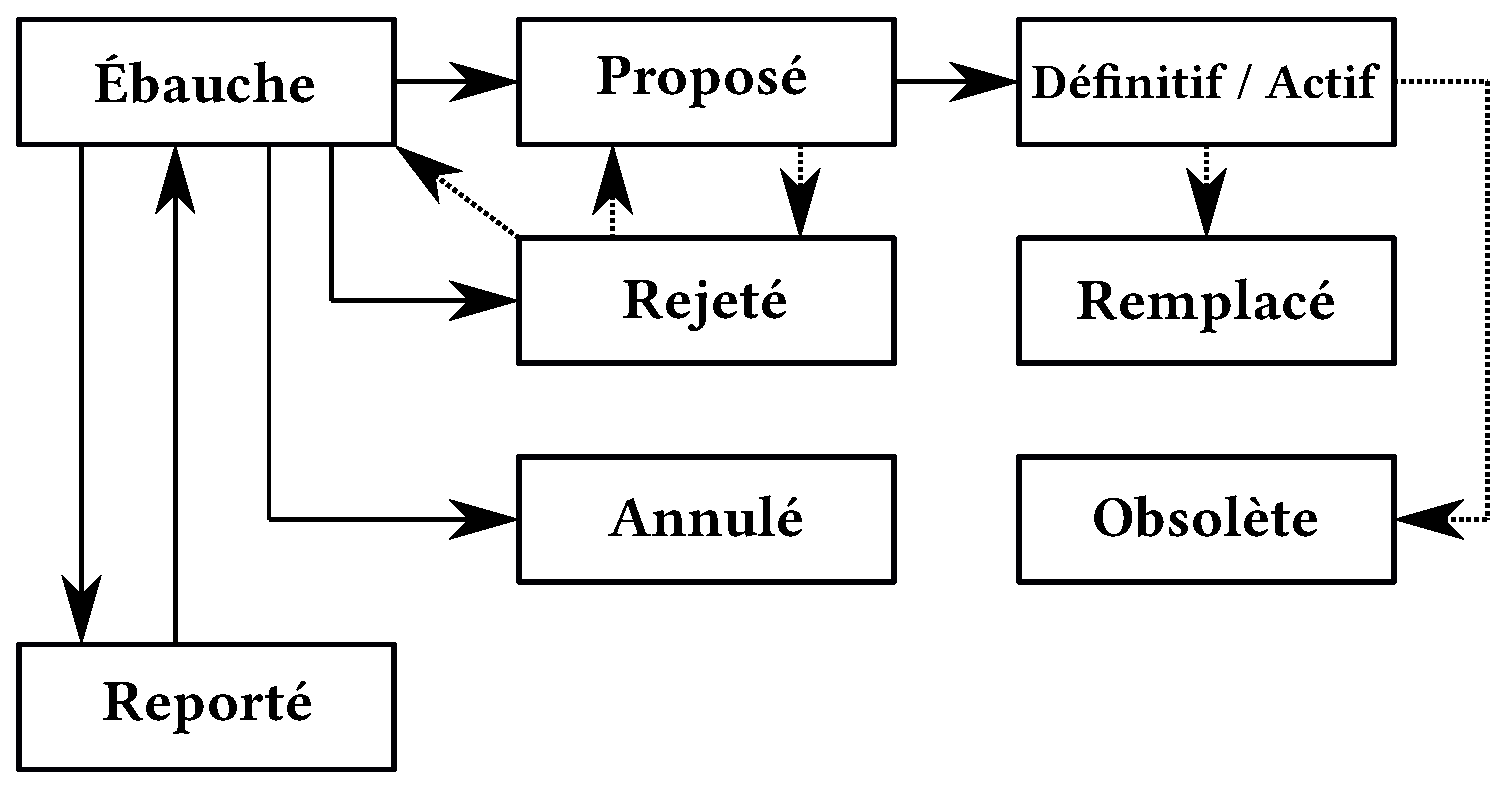
\includegraphics[scale=0.29]{img/bip-process-fr.eps}
  \caption{Schéma de la procédure d'adoption d'un BIP, inspiré du BIP-1.}
\end{figure}

% Utilisation des BIP pour les autres protocoles
Notez que ces documents sont utilisés pour BTC mais également pour d'autres protocoles. Par exemple, les BIP décrivant le fonctionnement des portefeuilles (BIP-32, BIP-39, BIP-44) sont valides pour la grande majorité des cryptomonnaies. Le SLIP-44 recense les cryptomonnaies compatibles avec le BIP-44\sendnote{\url{https://github.com/satoshilabs/slips/blob/master/slip-0044.md}}.

% Autres systèmes de propositions
Les autres protocole cryptoéconomiques disposent même parfois de leurs propres systèmes de proposition. Ethereum utilise les EIP (\eng{Ethereum Improvement Proposals}), Bitcoin Cash les CHIP\sendnote{\url{https://bch.info/en/chips}} (\eng{Cash Improvement Proposals}), Litecoin les LIP\sendnote{\url{https://github.com/litecoin-project/lips}}, etc.

\section*{La vérification des règles de consensus}
\addcontentsline{toc}{section}{La vérification des règles de consensus}

Bitcoin se base sur un réseau public d'ordinateurs accessible librement sur Internet. Ce réseau suit un modèle pair-à-pair, c'est-à-dire un modèle dans lequel tous les membres du réseau, appelés des nœuds, possèdent les mêmes privilèges. Ce sont ces nœuds qui s'assurent que les règles de consensus sont respectées. Si un bloc est invalide (en contenant une transaction invalide par exemple), alors il est rejeté par les nœuds appliquant les règles.

Dans Bitcoin, le rôle des nœuds est d'entretenir une copie du registre des transactions (la fameuse chaîne de blocs) et, ce faisant, de s'assurer de la validité des transactions et des blocs. Pour cela, ils communiquent avec les autres nœuds du réseau et relaient les nouvelles transactions et les nouveaux blocs, qui émanent respectivement des utilisateurs et des mineurs.

% Vérification complète
La vérification des règles de consensus peut être complète. Dans ce cas, on utilise parfois le pléonasme «~nœuds complets~» ou «~\eng{full node}~» pour insister sur le fait qu'ils vérifient l'intégralité de la chaîne. Ils téléchargent l'intégralité de la chaîne de blocs, vérifient les règles de consensus et relaient les blocs et les transactions. C'est une charge~: \textcolor{darkgray}{en avril 2023, la chaîne de Bitcoin pesait environ 480~Go de données et l'ensemble des UTXO plus de 4 Go, la zone mémoire des transactions est limitée à 100~Mo. La taille moyenne des blocs minés toutes les 10 minutes était de 1,3~Mo avant janvier 2023, et gravite aujourd'hui autour de 2~Mo.}

% Nœuds réduits
Les nœuds réduits (\eng{pruned nodes}), qui conservent l'état du réseau mais pas l'entièreté de la chaîne, sont des nœuds à part entière puisqu'ils ont vérifié la conformité des règles sur l'intégralité de la chaîne. Ils ne sont juste pas en mesure d'accéder à l'historique de la chaîne précédant une certaine date.

% Vérification partielle
La vérification peut aussi être partielle, auquel cas on peut parler de client léger (parler de nœud est abusif). Cela est utile pour les personnes qui n'ont pas l'intérêt de faire tourner un nœud complet. C'est par exemple le cas dans les logiciels de hachage (mettant en œuvre Stratum) et dans les portefeuilles légers. Ils utilisent en particulier une méthode conceptualisée dans le livre blanc de Bitcoin en 2008~: la vérification de paiement simplifiée\sendnote{Satoshi Nakamoto décrivait la vérification de paiement simplifiée comme suit~:

\begin{quote}
\footnotesize «~Il est possible de vérifier les paiements sans faire fonctionner un nœud complet du réseau. Un utilisateur a seulement besoin de conserver une copie des entêtes des blocs de la plus longue chaîne de preuves de travail, qu'il peut obtenir en interrogeant les nœuds du réseau jusqu'à ce qu'il soit convaincu qu'il possède la plus longue chaîne, et obtenir la branche de Merkle liant la transaction au bloc dans lequel elle est horodatée. Il ne peut pas vérifier la transaction par lui-même, mais en la reliant à un endroit de la chaîne, il peut voir qu'un nœud du réseau l'a acceptée, et les blocs ajoutés après le confirment.~»
\end{quote}
(Satoshi Nakamoto, \emph{Bitcoin : un système d'argent liquide électronique pair-à-pair}, 31 octobre 2008)}.

% Vérification de paiement simplifiée
La vérification de paiement simplifiée (nommée en anglais \eng{Simplified Payment Verification} et abrégée en SPV) est une méthode astucieuse, conceptualisée dès les origines, qui permet aux utilisateurs néophytes et occasionnels de pouvoir interagir facilement avec le protocole sans devoir gérer un nœud complet, ni devoir faire aveuglément confiance à un dépositaire. Elle permet de réduire considérablement la charge des portefeuilles légers.  % contribue au succès de Bitcoin

% Description de la vérification
La vérification de paiement simplifiée se base sur la façon dont les blocs de transactions sont chaînés et structurés comme on a pu le voir dans le chapitre~\ref{ch:confirmation}. Premièrement, la chaîne de preuve de travail n'est pas à proprement parler une chaîne de blocs, mais une chaîne d'entêtes. Cela fait que les clients légers n'ont qu'à conserver cette chaîne des entêtes pour déterminer la chaîne possédant le plus de travail accumulé. Puisque chaque entête pèse 80 octets, la taille des données à conserver reste modeste pour des appareils modernes~: elle augmente d'environ 4~Mio par an, \textcolor{darkgray}{ce qui représente un peu plus de 60~Mio en avril 2023}.

Deuxièmement, les transactions sont agencées dans un arbre de Merkle, de sorte que les clients légers peuvent se contenter de demander les informations liées à la branche qui les intéressent pour s'assurer de la confirmation d'une de leurs transactions. Le nombre d'empreintes à obtenir et de hachages à effectuer dépend du logarithme binaire ($\log_{2}$) du nombre de transactions présentes dans le bloc. Pour un bloc de 3000 transactions (moyenne haute sur BTC), la charge correspond à demander 12 empreintes de 32 octets et à calculer 12 hachages pour procéder à la vérification.

% Défauts de fiabilité, de confidentialité et de vérification
Cette vérification simplifiée permet d'alléger la charge des portefeuilles, mais elle présente quelques défauts. D'abord, elle manque de fiabilité~: les nœuds ne peuvent pas mentir en inventant une transaction, mais peuvent omettre de transmettre des informations nécessaires. Ce défaut peut être partiellement contrebalancé en augmentant la diversité des connexions sur le réseau. De plus, la vérification est vulnérable si la chaîne est attaquée par une entité disposant de la puissance de calcul majoritaire\sendnote{Ce cas a été décrit par Satoshi Nakamoto dans le livre blanc :

\begin{quote}
\footnotesize «~De ce fait, la vérification est fiable tant que les nœuds honnêtes contrôlent le réseau, mais est plus vulnérable si le réseau est maîtrisé par un attaquant. Alors que les nœuds du réseau peuvent vérifier les transactions par eux-mêmes, la méthode simplifiée peut être trompée par des transactions forgées par l'attaquant aussi longtemps que celui-ci maîtrise le réseau. Une stratégie pour se protéger serait d'accepter les alertes des nœuds du réseau lorsqu'ils détectent un bloc invalide, invitant le logiciel de l'utilisateur à télécharger le bloc complet et les transactions suspectes pour confirmer l'incohérence. Les entreprises qui reçoivent fréquemment des paiements voudront probablement toujours faire fonctionner leurs propres nœuds afin d'obtenir une sécurité plus indépendante et une vérification plus rapide.~»
\end{quote}
(Satoshi Nakamoto, \eng{Bitcoin: A Peer-to-Peer Electronic Cash System}, 31 octobre 2008.)

Les alertes décrites par Satoshi sont aujourd'hui appelées preuves de fraude mais sont toujours en phase de développement.}.

% Défaut de confidentialité
Ensuite, la vérification simplifiée possède aussi une  de confidentialité, en exigeant que le client léger fasse des requêtes auprès des nœuds du réseau et leur dévoile par conséquent son activité transactionnelle\sendnote{Une façon de remédier partiellement à ce problème est d'accroître le nombre d'informations demandées pour dissimuler les informations essentielles. Une première façon de procéder est de mettre en place des filtres de Bloom décrits dans le BIP-37. Il existe également Neutrino, décrit dans le BIP-157 et le BIP-158, qui fait usage du codage de Golomb-Rice et demande une plus grande bande passante.}.

% Défaut de vérification
Enfin, elle présente un défaut de vérification, en étant par définition partielle. Toutes les règles de consensus ne sont pas vérifiées, ce qui fait que les nœuds complets peuvent convenir d'un changement de règle qui ne sera pas remarqué par le client léger. Par exemple, les clients SPV ne vérifient pas les contraintes appliquées sur la taille des blocs, et le réseau pourrait donc subir une modification de cette limite sans qu'ils s'en rendent compte. C'est ce qui explique la stratégie des promoteurs de SegWit2X en 2017, qui prévoyaient de doubler la taille limite des blocs sans protection contre la rediffusion afin que les portefeuilles à vérification de paiement simplifiée suivent simplement la chaîne la plus longue\sendnote{Voir par exemple le courriel de Mike Belshe du 8 octobre 2017 où il déclare~: «~Aujourd'hui, nous sommes en bonne voie pour déployer segwit2x avec une grande majorité de mineurs qui le signalent encore. En plus de cela, 99,94~\% des nœuds et des clients SPV suivront automatiquement la chaîne la plus longue (segwit2x).~» -- Mike Belshe, \eng{[Bitcoin-segwit2x] Strong 2-Way Replay Protection}, \wtime{08/10/2017 20:16:02 UTC}~: \url{https://lists.linuxfoundation.org/pipermail/bitcoin-segwit2x/2017-October/000323.html}.}. % automatically follow that longest chain (segwit2x)

% Avis de Satoshi
Satoshi pensait\sendnote{Satoshi Nakamoto a conservé cette vision jusqu'à son départ, comme en témoigne son courriel à Mike Hearn du 29 décembre 2010~:

\begin{quote}
\footnotesize «~Un jour, lorsque nous aurons des implémentations fonctionnant uniquement en mode client, la taille de la chaîne de blocs n'aura plus beaucoup d'importance. D'ici là, tant que tous les utilisateurs ont toujours à télécharger la chaîne de blocs entière pour commencer, il est bon de pouvoir la maintenir à une taille raisonnable.~»
\end{quote} % "Eventually when we have client-only implementations, the block chain size won't matter much. Until then, while all users still have to download the entire block chain to start, it's nice if we can keep it down to a reasonable size."
(Satoshi Nakamoto, \eng{Re: More BitCoin questions}, \wtime{29/12/2010 21:42 UTC}~: \url{https://plan99.net/~mike/satoshi-emails/thread3.html})} que le système pourrait perdurer avec une vérification centralisée entre les mains de quelques nœuds vérificateurs (dont les mineurs) et que le reste des utilisateurs feraient usage des clients légers. Dans sa première réponse à James A. Donald en novembre 2008, il indiquait ainsi~:

\begin{quote}
«~Bien avant que le réseau n'atteigne cette taille, les utilisateurs pourront utiliser la vérification de paiement simplifiée (section 8) pour contrôler les doubles dépenses, ce qui ne nécessite que la chaîne des entêtes de bloc, soit environ 12~Ko par jour. Seules les personnes essayant de créer de nouvelles pièces auront besoin de faire fonctionner des nœuds de réseau.\sendnote{Satoshi Nakamoto, \eng{Re: Bitcoin P2P e-cash paper}, \wtime{03/11/2008, 01:37:43 UTC}~: \url{https://www.metzdowd.com/pipermail/cryptography/2008-November/014815.html}.}~»
\end{quote} % Long before the network gets anywhere near as large as that, it would be safe for users to use Simplified Payment Verification (section 8) to check for double spending, which only requires having the chain of block headers, or about 12KB per day.  Only people trying to create new coins would need to run network nodes.

En cela, il se trompait. La vérification des règles de consensus a besoin d'être intégrale pour que celles-ci soient appliquées.

% Utilité systémique de cette vérification
C'est donc au niveau du nœud complet que se joue cette vérification, Cette réalité est parfois retranscrite par l'adage «~pas ton nœud, pas tes règles\sendnote{L'adage «~\eng{not your node, not your rules}~» a été naturellement calqué sur l'adage «~\eng{not your keys, not your coins}~» (voir par exemple ce tweet de Udi Wertheimer~: \url{https://twitter.com/udiWertheimer/status/936215582487261184}). Il a été popularisé par le panel du même nom lors de la conférence Understanding Bitcoin, le 5 avril 2019~: \url{https://www.youtube.com/watch?v=jwaKVIEm-rI}. Le projet RaspiBlitz en a fait son slogan en 2020~: \url{https://github.com/rootzoll/raspiblitz/blob/bbeb5b21a982eeeb93306537e0aca2474bd23e03/README.md}.}~». Ne faites pas confiance, vérifiez~! Tout comme une langue résulte des choix que font ses locuteurs (n'en déplaise à l'Académie Française), un protocole informatique résulte des règles appliquées par les nœuds complets. Cette vérification joue donc un rôle crucial dans la détermination du protocole.

\section*{Les hard forks}
\addcontentsline{toc}{section}{Les hard forks}

Avant de voir comment est spécifiquement déterminé le protocole, intéressons-nous aux modifications des règles de consensus et comment elles se manifestent. Les modifications des règles de consensus peuvent être rangées dans deux catégories~: les \eng{hard forks}, mises à niveau brutes et incompatibles, et les soft forks, qui présentent une certaine rétrocompatibilité.

% Polysémie du mot fork
Le mot \eng{fork} est un terme anglais signifiant «~embranchement~», «~bifurcation~» ou «~fourche~». Dans Bitcoin, il existe une polysémie à son sujet (le terme possède quatre significations différentes), ce qui peut prêter à confusion.

% Fork logiciel
Comme on l'a dit, le terme de fork est d'abord utilisé dans le développement logiciel, notamment dans le cadre du logiciel libre qui autorise et encourage ce type de pratique. Il désigne la création un programme dérivé du code source d'un programme existant et aussi, par abus de langage, le programme dérivé en lui-même. En ce sens, l'implémentation de référence peut subir un embranchement, créant un logiciel alternatif. Ce logiciel peut respecter les règles de consensus (comme par exemple Bitcoin Knots), mais il peut aussi les faire dévier, en créant un nouveau protocole qui partage l'historique de la chaîne (Bitcoin ABC, devenu Bitcoin Cash Node) ou non (Litecoin).

% Embranchement commun de la chaîne
Le fork peut ensuite désigner l'embranchement commun de la chaîne de blocs, par analogie avec le développement logiciel. La chaîne de blocs n'est en effet pas une structure linéaire, mais une «~structure en forme d'arbre\sendnote{Satoshi Nakamoto, code source de la version 0.1 du logiciel Bitcoin~: \url{https://github.com/trottier/original-bitcoin/blob/4184ab26345d19e87045ce7d9291e60e7d36e096/src/main.h\#L1001-L1008}.}~» qui peut posséder de multiples branches de blocs, pareillement compatibles avec les règles de consensus acceptées par le réseau, la sélection de la branche correcte se faisant par la plus longue (possédant le plus de travail accumulé). Ce type d'embranchement se produit régulièrement dans Bitcoin de manière tout à fait normale et bénigne, lorsque deux mineurs trouvent simultanément un bloc différent de leur côté, et est résolu lorsqu'un nouveau bloc est trouvé.

% Scission
Le fork peut aussi se rapporter à une scission de la chaîne de blocs causée par une incompatibilité des règles de consensus. On parle alors de hard fork, c'est-à-dire littéralement d'«~embranchement dur~». Cette scission est généralement permanente dans le sens où les deux branches ne peuvent pas se réconcilier par le mécanisme de consensus de Nakamoto, sauf dans un cas très précis~: si les règles de la branche majoritaire forment une restriction des règles de la branche minoritaire. Les deux chaînes résultantes sont, à terme, vouées à exister sur des réseaux séparés.

% Hard fork / soft fork
Enfin, le terme de fork peut, par métonymie, désigner une modification des règles de consensus, qui est toujours susceptible de provoquer une scission de chaîne et une séparation du réseau. Une restriction des règles de consensus est appelée un soft fork, littéralement «~embranchement doux~», en vertu de sa capacité à ne résulter en une branche unique. Toute autre modification des règles de consensus, qu'il s'agisse d'une extension ou d'une modification strictement incompatible, est appelée un hard fork, en référence à sa propension à créer une scission de chaîne. C'est de ces deux modifications dont nous voulons parler ici.\sendnote{Notez que les concepts sont liés. Ainsi, un fork logiciel (copie et modification) peut implémenter un fork des règles de consensus (hard fork ou soft fork) qui finira par créer un fork de chaîne (scission).}

%
Le hard fork est le concept le plus ancien chronologiquement par rapport au soft fork. Il était auparavant qualifié de «~changement incompatible\sendnote{Voir par exemple David François, \eng{Re: Small protocol changes for flexibility}, \wtime{07/12/2010 15:08:02 UTC}~: \url{https://bitcointalk.org/index.php?topic=894.msg27757\#msg27757}.}~». Le hard fork est une modification non restrictive des règles de consensus. Il provoque un conflit sur le réseau entre les nœuds qui appliquent les anciennes règles et les nœuds qui appliquent les nouvelles.

% Hard fork extensif
Un hard fork peut être extensif, c'est-à-dire élargir les règles de consensus sur les blocs et les transactions. Les anciens peuvent ainsi produire des blocs valides sur la nouvelle chaîne, mais pas l'inverse. L'exemple typique de ce genre de hard fork est l'augmentation de la taille limite des blocs, qui consiste à accepter des blocs ayant une taille ou un poids plus grand. Par exemple, un passage de 1~Mo à 2~Mo ou de 4~MWU à 8~MWU.

\textcolor{brown}{schéma hard fork extensif d'augmentation de la taille limite de blocs, branche majoritaire}

Dans le cas où le hard fork extensif n'est pas soutenu par une majorité de la puissance de calcul du réseau, celui-ci risque de ne pas avoir lieu. En effet, les blocs de la branche imposant une taille plus petite sont entièrement compatibles avec les nouvelles règles, de sorte que, si elle est plus longue, c'est elle qui sera sélectionnée comme la branche correcte. C'est pour éviter cette situation problématique que les hard forks sont généralement bilatéraux.

% Hard fork bilatéral
Mais il peut aussi être bilatéral en créant une incompatibilité totale entre les nouvelles règles et les anciennes. Il peut s'agir d'une règle ajoutée comme l'exigence que le premier bloc de l'embranchement inclue un changement incompatible. Dans notre cas de l'augmentation de la chaîne de blocs, il s'agirait d'imposer au premier bloc d'être strictement plus gros que la taille limite précédente. Cette règle supplémentaire est appelée protection contre la destruction par recoordination (\eng{wipeout protection}).

\textcolor{brown}{schéma hard fork bilatéral d'augmentation de la taille limite de blocs, branche minoritaire}

Un autre exemple est le changement de l'algorithme de signature des transactions, qui rend l'intégralité des transactions signées et des blocs non vides strictement incompatibles. Ce changement a pour effet de permettre en plus une protection contre la rediffusion des transactions (\eng{replay protection}), dans le cas où deux chaînes concurrentes persisteraient.

% Deux hard forks, deux intentions
Deux situations peuvent découler d'un hard fork~: soit la quasi-totalité de l'économie procède au changement, auquel cas une seule chaîne subsiste~; soit l'économie se fragmente, auquel cas les deux chaînes subsistent. La première situation est visée par le hard fork de mise à niveau qui n'a pas vocation à créer deux chaînes distinctes. La seconde est désirée par le hard fork contentieux, résultant d'une division de la communauté au sujet du changement. Le hard fork accidentel, créé par une modification non désirée des règles de consensus implicites, est écarté ici\sendnote{Le 11 mars 2013, le passage de la version 0.7 du logiciel à la version 0.8 implémentait la migration du système de base de données de Berkeley DB à LevelDB. Toutefois, il s'avérait que Berkeley DB faisait intervenir une limite par défaut (\eng{lock limit}) qui n'était pas présente dans LevelDB. Par conséquent, la migration constituait un hard fork accidentel et a provoqué un embranchement à partir du bloc 225~430 qui a duré environ 6 heures. La décision a finalement été prise de revenir à la version 0.7, invalidant la branche de 24 blocs minée du côté de la version 0.8, et de procéder à la migration quelques mois plus tard. -- Voir Vitalik Buterin, \eng{Bitcoin Network Shaken by Blockchain Fork}, 13 mars 2013~: \url{https://bitcoinmagazine.com/technical/bitcoin-network-shaken-by-blockchain-fork-1363144448}~; Gavin Andresen, \eng{BIP-50: March 2013 Chain Fork Post-Mortem}, ~: \url{https://github.com/bitcoin/bips/blob/master/bip-0050.mediawiki}. Une double dépense conséquente a été réalisée~: macbook-air, \eng{A successful DOUBLE SPEND US\$10000 against OKPAY this morning.}, \wtime{12/03/2013, 18:22:02 UTC}~: \url{https://bitcointalk.org/index.php?topic=152348.msg1616747\#msg1616747}.}.

% Hard fork de mise à niveau
Le hard fork de mise à niveau est un hard fork qui nécessite une synchronisation de la quasi-totalité de la communauté. Il résulte généralement en une seule chaîne, de sorte qu'on peut considérer que le protocole a été mis à niveau (alors qu'il s'agit essentiellement d'une utilisation économique qui passe d'un protocole à un autre). Il peut pour cela être extensif, même la bilatéralité est préférée pour des raisons de sécurité.

% Exemples de hard forks de mise à niveau
Le premier hard fork de mise à niveau connu est probablement l'ajout par Satoshi Nakamoto des codes opération \texttt{OP\_NOP} à la version 0.3.6 de Bitcoin en juillet 2010. L'augmentation de la taille des blocs était également pensée comme un hard fork de mise à niveau, notamment par Satoshi Nakamoto lui-même\sendnote{En octobre 2010, à la suite de la proposition de Jeff Garzik d'augmenter la limite directement à 7,168~Mo afin d'«~égaler le taux transactionnel moyen de PayPal~», Satoshi -- bien conscient qu'il s'agissait d'un correctif «~incompatible avec le réseau~» -- écrivait~:
\begin{quote}
\footnotesize «~[La mise à niveau] peut être introduite progressivement, par exemple~:

if (blocknumber > 115000)
  maxblocksize = largerlimit

Elle peut commencer à être intégrée dans les versions bien avant, de sorte qu'au moment où elle atteint le numéro de bloc et entre en vigueur, les anciennes versions qui ne l'ont pas sont déjà obsolètes.

Lorsque nous approchons du numéro de bloc limite, je peux envoyer une alerte aux anciennes versions pour qu'elles sachent qu'elles doivent effectuer une mise à jour.~»
\end{quote}
(Satoshi Nakamoto, \eng{Re: [PATCH] increase block size limit}, \wtime{04/10/2010 19:48:40 UTC}~: \url{https://bitcointalk.org/index.php?topic=1347.msg15366\#msg15366})}, jusqu'au hard fork contentieux de Bitcoin Cash en 2017. Celle-ci était envisagée par Satoshi Nakamoto lui-même.

En dehors de BTC, les mises à niveaux par hard fork sont nombreuses, notamment en raison d'une économie moins grande et~/~ou plus centralisée. On peut citer les cas de Bitcoin Cash, de Monero, d'Ethereum Classic et d'Ethereum, où des mises à niveau de ce type sont réalisées régulièrement.

% Hard fork contentieux
Le hard fork contentieux est un hard fork visant à créer une nouvelle chaîne délibérément. Il est issu d'une dissension dans la communauté, si forte qu'elle pousse à la sécession. Il est généralement bilatéral.

% Exemples de hard forks contentieux
Le premier exemple de hard fork contentieux majeur est celui qui a eu lieu sur Ethereum en juillet 2016, dans le contexte du piratage de TheDAO. Ce hard fork consistait à reprendre les fonds du pirate par un «~changement d'état irrégulier~». Celui-ci était rendu bilatéral par la règle imposant aux 10 premiers blocs d'inclure la chaîne de caractères \texttt{dao-hard-fork}. Puisque la majorité économique se trouvait du côté de l'annulation, la chaîne altérée a gardé le nom d'Ethereum et le sigle boursier ETH, tandis que l'autre chaîne a pris le nom d'Ethereum Classic et le sigle boursier ETC.\sendnote{Simon Polrot, \emph{The DAO~: post mortem}, 24 janvier 2017~: \url{https://www.ethereum-france.com/the-dao-post-mortem/}~; Casey Detrio, \eng{EIP-779: Hardfork Meta: DAO Fork}, 26 novembre 2017~: \url{https://eips.ethereum.org/EIPS/eip-779}.}

Le second exemple de hard fork contentieux est celui qui a mené à la création de Bitcoin Cash en août 2017 suite au débat sur la scalabilité et à la guerre des blocs. Ce hard fork n'intégrait pas SegWit, augmentait la taille limite des blocs à 8~Mo et améliorait l'algorithme de signature. Il était rendu bilatéral par une règle qui imposait au bloc suivant l'activation d'avoir une taille au bloc suivant d'avoir une taille strictement supérieure à 1~Mo. Il offrait aussi \emph{de facto} une protection contre la rediffusion des transactions. Ce changement ayant dû se faire sans l'accord de la majorité économique, la chaîne qui ne modifiait pas les règles a pu conserver le nom de Bitcoin et le sigle boursier BTC, tandis que la nouvelle chaîne a dû adopter un nouveau nom, Bitcoin Cash, et un nouveau sigle BCH.\sendnote{Ludovic Lars, \emph{Bitcoin Cash~: la branche minoritaire issue du débat sur la scalabilité}, 30 janvier 2022~: \url{https://journalducoin.com/analyses/bitcoin-cash-branche-minoritaire-debat-scalabilite/}~; \eng{BCH-UAHF: Bitcoin Cash User-Activated Hard Fork}, 24 juillet 2017~: \url{https://reference.cash/protocol/forks/bch-uahf}.}

\textcolor{brown}{schéma scission Bitcoin / Bitcoin Cash}

% Ajustement de la difficulté
Notez qu'un tel hard fork peut devoir avoir à modifier l'algorithme d'ajustement de difficulté. En effet, si la puissance de calcul est trop faible pour le soutenir, il est possible que l'ajustement n'arrive pas à terme. C'est pour cette raison que Bitcoin Cash a dû implémenter un \eng{Emergency Difficulty Adjustment} (EDA) qui a permis de procéder à l'adaptation sur une période plus courte. Ethereum Classic n'a cependant pas dû le faire, car l'ajustement sur Ethereum avait déjà lieu à tous les blocs.

\section*{Les soft forks}
\addcontentsline{toc}{section}{Les soft forks}

% Définition
Le soft fork est une restriction des règles de consensus. Il consiste par essence à rendre l'ensemble des blocs et des transactions valides plus petit, en ajoutant une règle ou en modifiant une règle existante de façon plus restrictive. L'exemple typique de ce genre de fork est la diminution de la taille limite des blocs. L'ajout de la limite explicite des 1~Mo en octobre 2010 était ainsi un soft fork.

% Application par la puissance de calcul
Le soft fork peut être appliqué en conservant une seule et même chaîne. S'il est imposé par la majorité de la puissance de calcul du réseau, il n'y a aucun risque de scission. En effet, l'ensemble des blocs créés par les mineurs appliquant les nouvelles règles est entièrement compatible avec les anciennes règles, de sorte que la branche appliquant les nouvelles règles sera considérée comme la branche correcte par tous les nœuds si elle est majoritaire.

\textcolor{brown}{schéma soft fork de diminution de la taille limite de blocs, branche majoritaire}

% Origine
Le concept de soft fork est postérieur à celui de hard fork. Il a été formellement découvert par Gavin Andresen en octobre 2011 qui, suite à son étude de la proposition d'ajout du code opération \texttt{OP\_EVAL} par Nicolas van Saberhagen\sendnote{Nicolas van Saberhagen, \eng{OP\_EVAL proposal}, \wtime{02/10/2011 00:49:19 UTC}~: \url{https://bitcointalk.org/index.php?topic=46538.msg553689\#msg553689}.}, s'est aperçu que la mise à niveau pouvait se faire grâce aux code opération \texttt{OP\_NOP1} sans nécessairement provoquer de scission\sendnote{«~Je lis probablement mal le code, mais je pense que OP\_EVAL ne provoquerait pas de scission de blockchain~!~» s'est exprimé Gavin Andresen sur IRC. -- \#bitcoin-dev IRC logs, 2 octobre 2010~: \url{https://web.archive.org/web/20131201200245/http://bitcoinstats.com/irc/bitcoin-dev/logs/2011/10/02}.}.

% Codes opération
Les codes opération \texttt{OP\_NOP} sont des instructions du langage de script de Bitcoin qui ont été ajoutés dans le code par Satoshi en juillet 2010 avec pour seul commentaire «~expansion\sendnote{\url{https://sourceforge.net/p/bitcoin/code/119/}}~». Le changement a été rendu effectif avec la version 0.3.6 du logiciel qui corrigeait également le 1 RETURN bug, publiée le 29 juillet\sendnote{Satoshi Nakamoto, \eng{*** ALERT *** Upgrade to 0.3.6}, \wtime{29/07/2010 19:13:06 UTC}~: \url{https://bitcointalk.org/index.php?topic=626.msg6451\#msg6451}.}. Leur rôle est initialement muet~: s'ils sont présents dans un script, ils ne font rien mais ils n'invalident pas la transaction non plus. Cela entraîne qu'on peut modifier le comportement de ces codes opération sans rendre les scripts incompatibles avec les anciennes règles de consensus. Cette caractéristique indique que que Satoshi avait, sinon compris, au moins deviné le mécanisme du soft fork.

% Échange sur IRC
% 16:40	gavinandresen	I'm probably reading the code wrong, but I think OP_EVAL wouldn't cause a blockchain split!
% 18:59	gmaxwell	wow. Gavin's point that EVAL can be done without a split blew my mind.
% 21:23	gmaxwell	You can also make the new code keep the old behavior for blocks before a certian height.
% 21:24	gmaxwell	So you can set the actual switch point at some point in the future.
% 21:25	gmaxwell	(so that you have time to actually achieve >>50% hashpower behind the change)
% 21:27	gmaxwell	e.g. make and backport a patch which will agressively not forwardward txn with the reserved NOP until block X, and after X start applying the new validation rules but only to future blocks. Then so long has >>50% hashpower is running this patch by block X there is no lasting fork created.

% Caractère postcompatible
Le soft fork possède un caractère «~rétrocompatible~» -- ou postcompatible à proprement parler, la compatibilité étant ascendante et non descendante -- dans le sens où les anciennes versions du logiciel peuvent continuer d'interagir avec le système. En effet, les nœuds non miniers suivant les anciennes règles continuent de voir les blocs produits comme valides. Cette caractéristique est un avantage majeur par rapport au hard fork.

% La rétrocompatibilité, ou compatibilité descendante, est la compatibilité d'un produit vis-à-vis de ses anciennes ou précédentes versions ; la compatibilité ascendante ou postcompatibilité est la compatibilité d'un produit vis-à-vis des versions plus récentes, voire encore en phase de conception.

% Non-optionnalité
Mais cette compatibilité ascendante ne veut pas dire qu'un soft fork est «~doux~». Il possède un côté pernicieux dans le sens où il rend la modification difficile à appréhender. D'abord, il n'est pas optionnel. S'il est appliqué par la majorité de la puissance de calcul, un soft fork s'apparente en effet à une attaque de censure pour les utilisateurs appliquant les anciennes règles. Le soft fork possède donc un caractère coercitif que le hard fork n'a pas.

% Irréversibilité
Puis, le soft fork est difficilement réversible. Les fonctionnalités ajoutées ne peuvent pas être désactivées simplement~: une fois adopté, il n'y a pas de retour en arrière facile. Les développeurs de Bitcoin SV ont ainsi désactivé P2SH en février 2020 exposant les utilisateurs les moins attentifs à des vols\sendnote{Jon Southurst, \eng{Final Genesis specs released—bye P2SH}, 10 janvier 2020~: \url{https://coingeek.com/final-genesis-specs-released-bye-p2sh/}.}.

% Non-limitation
Ensuite, le soft fork n'est pas limité quant à ce qu'il peut faire. Il peut augmenter la limite effective de taille des blocs (via un bloc auxiliaire aussi appelé bloc d'extension\sendnote{\url{https://bitcointalk.org/index.php?topic=283746.msg3036293\#msg3036293}~; \url{https://lists.linuxfoundation.org/pipermail/bitcoin-dev/2015-May/008356.html}} ou soft fork généralisé\sendnote{ZoomT, \eng{Increasing the blocksize as a (generalized) softfork.}, \wtime{20/12/2015 11:12:48 UTC}~: \url{https://bitcointalk.org/index.php?topic=1296628.msg13305141\#msg13305141}.}). Ce bloc d'extension peut également inclure des fonctionnalités supplémentaires (comme MimbleWimble dans Litecoin). Il peut même modifier la politique monétaire du protocole en redéfinissant l'unité de base\sendnote{La façon dont un soft fork peut introduire de l'inflation dans Bitcoin a été exposée par le développeur Peter Todd en 2016. -- Peter Todd, \eng{Forced Soft Forks}, 18 janvier 2016~: \url{https://petertodd.org/2016/forced-soft-forks}.}.

% Complexité
Enfin, le soft fork, s'il est profond, crée une complexité supplémentaire, liée aux contraintes de son application. En effet, il ajoute de nouvelles exceptions aux règles de consensus, ce qui génère de la dette technique\sendnote{Ward Cunningham, «~The WyCash Portfolio Management System~», \eng{Addendum to the Proceedings of OOPSLA 1992}, octobre 1992~: \url{https://dl.acm.org/doi/pdf/10.1145/157710.157715}.} pour les développeurs.

% (L'abominable) SegWit
L'archétype du soft fork profond et complexe a été la mise à niveau SegWit, ou \eng{Segregated Witness}, qui consistait à déplacer les données de signature des transactions (appelées témoin ou \eng{witness}) vers une structure de données séparée (\eng{segregated}) afin de supprimer la malléabilité des transactions. Cette mise à niveau, qui a eu lieu en le 24 août 2017, devait être initialement un hard fork, avant que le développeur luke-jr ne décrive en 2015 comment en faire un soft fork\sendnote{Aaron van Wirdum, \eng{The Long Road to SegWit: How Bitcoin's Biggest Protocol Upgrade Became Reality}, 23 août 2017~: \url{https://bitcoinmagazine.com/technical/the-long-road-to-segwit-how-bitcoins-biggest-protocol-upgrade-became-reality}.}. La rétrocompatibilité était assurée par la liaison du témoin au bloc via un arbre de Merkle dont la racine était placée dans la transaction de récompense et par l'utilisation de sorties transactionnelles dépensables par n'importe qui (\eng{anyone-can-spend}). Outre la correction du problème de malléabilité, elle a instauré un système de versionnage (qui a permis l'intégration de Schnorr-Taproot par la suite) et a modérément augmenté la capacité transactionnelle du réseau, de sorte que la taille effective des blocs pouvait dépasser 1~Mo, jusqu'à 4~Mo en théorie. Elle a également ajouté quatre nouveaux types d'adresse au protocole.

% Méthodes d'activation
De plus, le soft fork requiert la majorité de la puissance de calcul du réseau pour préserver son intérêt. S'il n'est pas suivi à moyen terme par 51~\% de la puissance de calcul, alors son application provoque une scission. C'est ce qui explique pourquoi l'activation par les mineurs est généralement préférée à l'activation par les utilisateurs, même si le pouvoir de décision revient à ces derniers comme on le verra.

% Soft fork activé par les utilisateurs
D'une part, le soft fork activé par les utilisateurs (en anglais \eng{user activated soft fork} ou UASF) consiste à implémenter le soft fork dans le code source du logiciel de sorte à ce qu'il rentre en application à une hauteur de bloc ou à un horodatage donné. Cette méthode s'appuie sur la confiance que l'économie appliquant la mise à niveau sera largement majoritaire et que l'activité minière suivra à moyen terme en raison d'une récompense de bloc plus élevée.

% Soft fork activé par les mineurs
D'autre part, le soft fork activé par les mineurs (en anglais \eng{miner activated soft fork} ou MASF) consiste à faire dépendre l'activation du signalement des mineurs au sein des blocs validés. Il est activé lorsqu'un certain seuil de signalement (95~\% par exemple) est dépassé. Cette méthode, dont la procédure a été notamment décrite dans le BIP-9, permet de s'assurer autant que possible que les mineurs appliquent la mise à niveau et qu'il ne subsiste qu'une seule chaîne.

% UAHF / MAHF
La même distinction existe dans l'activation des hard forks, mais celle-ci peu de pertinence, la puissance de calcul ne pouvant pas empêcher la scission. Ainsi, le hard fork activé par les mineurs (MAHF), longtemps été soutenu par les partisans de l'augmentation de la taille limite des blocs, n'a pas d'intérêt particulier.

% Deux types de soft forks
Comme les hard forks, les soft forks peuvent être rangés en deux catégories plus ou moins distinctes~: le soft fork de mise à niveau et le soft fork contentieux.

% Soft fork de mise à niveau
Le soft fork est idéal pour mettre à niveau le protocole. Cela permet aux nœuds de ne pas se mettre à niveau tout de suite. Même s'il demande une certaine synchronisation, celle-ci n'est pas aussi contraignante que pour les hard forks.

% Exemples de soft forks de mise à niveau dans BTC
Dans BTC, le soft fork est ainsi privilégié par les développeurs depuis sa découverte. P2SH, l'obligation de spécifier l'empreinte du bloc dans la transaction de récompense (BIP-34) ou l'ajout d'un standard d'encodage des signatures (BIP-66). Les ajouts des codes opération \texttt{OP\_CHECKLOCKTIMEVERIFY} et \texttt{OP\_CHECKSEQUENCEVERIFY} permettant l'usage de verrous temporels dans le langage de scipt par l'utilisation respective des codes \texttt{OP\_NOP2} et \texttt{OP\_NOP3} ont également été des soft forks. Enfin, plus récemment, l'adoption de Schnorr-Taproot (ou Taproot pour faire court) a été également une mise à niveau par soft fork.

% Exemples de soft forks de mise à niveau dans LTC
Litecoin fait également usage de ce type de transition. Le protocole a notamment intégré SegWit en mai 2017, ainsi que Schnorr-Taproot et MimbleWimble (MWEB) en mai 2022.

% Soft fork contentieux
Le soft fork contentieux a pour objectif de contraindre la minorité de la communauté à suivre la majorité. S'il réussit, il n'y a qu'une seule chaîne, les opposants ayant le choix d'accepter les règles ou de procéder eux-mêmes à un hard fork. S'il échoue, il résulte en deux chaîne concurrentes.

% SegWit
SegWit est l'exemple typique d'un soft fork contentieux réussi. Il n'était pas approuvé par l'ensemble des acteurs importants (les partisans des gros blocs d'une part, les puristes du protocole comme Mircea Popescu d'autre part, s'y opposaient), mais il a recueilli un soutien majoritaire de sorte qu'il a pu perdurer et que les mécontents \eng{big blockers} ont dû migrer vers Bitcoin Cash.

% "Coinbase rule"
Un exemple de soft fork contentieux ayant échoué est la tentative de l'équipe de Bitcoin ABC d'imposer une redirection de 8~\% de la subvention de minage de Bitcoin Cash vers elle-même le 15 novembre 2020\sendnote{Amaury Séchet, \eng{Bitcoin ABC's plan for the November 2020 upgrade}, 6 août 2020~: \url{https://amaurysechet.medium.com/bitcoin-abcs-plan-for-the-november-2020-upgrade-65fb84c4348f}.}. Cette tentative, qui était un soft fork en raison du caractère restrictif, a provoqué la scission entre une branche majoritaire sans redirection (BCH) et une branche minoritaire avec, qui a été par la suite renommée en «~eCash~» (XEC).

% Supériorité du soft fork
Ainsi, le soft fork, qu'il soit approuvé à l'unanimité ou bien seulement par une majorité, est une méthode supérieure au hard fork. Bien qu'il soit parfois plus complexe, il permet de ne pas requérir une synchronisation de l'économie entière, cette dernière pouvant s'y adapter progressivement, ce qui est un bienfait non négligeable dans le cas d'un système ouvert et divers comme Bitcoin. Le signalement supermajoritaire des mineurs permet de minimiser le risque de scission et de conserver l'effet de réseau au maximum.

% % Meilleure méthode de mise à niveau
% Les soft forks ont ainsi des caractéristiques précises qui font qu'ils possèdent des avantages, mais aussi des inconvénients, par rapport aux hard forks. Si la mise à niveau est profonde, le hard fork a l'avantage d'être simple, tandis que le soft fork peut présenter une certaine complexité. Le hard fork requiert que l'ensemble du réseau se synchronise pour appliquer la mise à niveau, tandis que le soft fork ne demande qu'une synchronisation de la puissance de calcul majoritaire et une adaptation progressive de l'économie. De ce fait, la probabilité d'une scission est plus élevée dans le cas d'un hard fork que dans celui d'un soft fork qui aurait fait l'objet d'un signalement supermajoritaire des mineurs, ce qui permet la conservation de l'effet de réseau.

% Sacrifice du consentement
Mais cet avantage majeur se fait au prix d'un sacrifice~: celui de la clarté du consentement. Dans le cas du hard fork, le consentement est clair~: les personnes qui souhaitent la modification se retrouvent sur la chaîne qu'elles ont choisie. Dans le cas, du soft fork, le consentement est plus ambigu~: le fait d'opérer sur la chaîne n'indique pas nécessairement une acceptation active du changement, mais une résignation passive et un refus de réaliser un hard fork minoritaire. Comme l'écrivait brillamment Vitalik Buterin en mars 2017~:

\begin{quote}
«~Les soft forks favorisent clairement la coercition par rapport à la sécession d'un point de vue systémique, alors que les hard forks ont le penchant inverse.\sendnote{Vitalik Buterin, \eng{Hard Forks, Soft Forks, Defaults and Coercion}, 14 mars 2017~: \url{https://vitalik.ca/general/2017/03/14/forks_and_markets.html}.}~»
\end{quote} % Soft forks clearly institutionally favor coercion over secession, whereas hard forks have the opposite bias.

Ainsi, même s'ils sont supérieurs dans la plupart des cas, les soft forks ne doivent pas nécessairement être privilégiés dans toutes les situations.

\section*{Le pouvoir sur le protocole} % Le rôle central des commerçants
\addcontentsline{toc}{section}{Le pouvoir sur le protocole}

La détermination du protocole est un aspect majeur de Bitcoin. En effet, l'absence d'autorité centrale pose la question de la prise de décision~: puisqu'il n'y a personne pour ordonner quoi que ce soit, comment le protocole peut-il être choisi et modifié~? Il est donc nécessaire de repenser notre conception de la chose pour pouvoir la comprendre.

% Détermination économique
Tel que nous l'avons laissé entendre, la détermination du protocole est réalisée par l'économie. Puisque Bitcoin est un système économique, il est naturel que les règles qui le composent résultent du marché, et non d'un décret fixe passé ou d'une autorité centrale actuelle.

L'idée que l'économie permet de déterminer le protocole n'est pas nouvelle, et remonte au moins à la déclaration de Meni Rosenfeld qui écrivait dans une réponse sur Stack Overflow en juin 2012 qu'un changement du protocole nécessitait «~une majorité économique, c'est-à-dire l'adoption par les utilisateurs et les entreprises qui donnent de la valeur à la monnaie\sendnote{\url{https://bitcoin.stackexchange.com/questions/3945/how-could-the-bitcoin-protocol-be-changed-has-this-ever-occurred\#comment4983_3948}}~». Gavin Andresen lui-même avait mis en avant cette idée en mai 2015, alors que la question d'augmenter la taille limite des blocs se posait~: % "A change requires an economic majority - adoption by the users and businesses who give the currency value."

\begin{quote}
«~Si nous ne parvenons pas à un consensus ici, l'autorité ultime pour déterminer le consensus est le code utilisé par la majorité des commerçants, des plateformes d'échange et des mineurs.\sendnote{Gavin Andresen, \eng{[Bitcoin-development] Proposed alternatives to the 20MB step function}, \wtime{29/05/2015 12:39:30 UTC}, \url{https://lists.linuxfoundation.org/pipermail/bitcoin-dev/2015-May/008340.html}.}~»
\end{quote} % "Because if we can't come to consensus here, the ultimate authority for determining consensus is what code the majority of merchants and exchanges and miners are running."

Mais la clarté de cette conception n'est arrivée qu'après les évènements de la guerre des blocs, durant laquelle les mécanismes sous-jacents ont pu s'exprimer. Ce n'étaient pas les développeurs qui décidaient des règles, ce n'étaient pas les mineurs non plus, mais bien plutôt les utilisateurs, et plus précisément les \emph{commerçants}. Eric Voskuil écrivait ainsi en novembre 2018~:

\begin{quote}
«~Bitcoin ne repose pas sur un dépositaire, mais dans l'intérêt d'établir un principe général, on peut considérer l'ensemble de tous les commerçants comme le dépositaire collectif de Bitcoin.\sendnote{Eric Voskuil, \emph{Cryptoéconomie}, «~Principe de risque de garde~» (p. 34).}~»
\end{quote}

% Le pouvoir des commerçants
Les commerçants sont, au sens large, les personnes qui fournissent des biens, des services ou d'autres monnaies contre du bitcoin, à des prix acceptables sur le marché. Cette prestation se manifeste par les échanges effectifs avec des clients et se mesure au travers des recettes perçues. En cela, les commerçants contribuent à l'utilité du bitcoin, qui se mesure à la quantité de biens et de services qu'il permet d'acquérir, et par conséquent à l'importance économique de la chaîne\sendnote{Cette réalité avait été perçue en janvier 2010 par NewLibertyStandard, le premier commerçant de Bitcoin~: «~Toutes les personnes qui achètent ou vendent des biens en utilisant des bitcoins, y compris les changeurs, font progresser l'économie de Bitcoin~!~» -- NewLibertyStandard, \eng{Re: New Exchange Service: "BTC 2 PSC"}, \wtime{19/01/2010 08:06:15 UTC}~: \url{https://bitcointalk.org/index.php?topic=15.msg111\#msg111}.}. Par l'utilisation d'un nœud permettant de vérifier les règles de consensus, ils participent ainsi à la détermination du protocole en proportion de leur activité économique potentielle.

% Modifier le protocole
Parler d'un protocole unique qui changerait est une approximation~: en tant qu'ensemble de règles, les protocoles sont tous fixes, mais leur utilisation (et leur utilité) varie. Modifier le protocole consiste donc à constituer un nouveau protocole dont la chaîne résultante sera économiquement plus importante que toute autre branche concurrente, y compris celle liée au protocole originel\sendnote{Jeff Garzik écrivait très justement en octobre 2010 que «~l'effort visant à augmenter la limite du taux de transaction [était] le même que celui visant à modifier la nature fondamentale des bitcoins~: convaincre la grande majorité de se mettre à niveau~». -- Jeff Garzik, \eng{Re: [PATCH] increase block size limit}, \wtime{04/10/2010 18:33:55 UTC}~: \url{https://bitcointalk.org/index.php?topic=1347.msg15342\#msg15342}.}. Par exemple, SegWit a été un soft fork contentieux, mais le protocole résultant a été beaucoup plus valorisé que les protocoles concurrents (BTC pré-SegWit et Bitcoin Cash), de sorte qu'on peut dire que le protocole BTC a été mis à niveau par cette modification. % The effort to raise the transaction rate limit is the same as the effort to change the fundamental nature of bitcoins:  convince the vast majority to upgrade.

% Multiplicité des Bitcoins
Bitcoin-le-concept englobe par nature une multiplicité de protocoles, en raison de son caractère libre et ouvert. Il n'y a pas un seul protocole Bitcoin, mais plusieurs, comme il y a plusieurs distributions Linux ou plusieurs dollars. Et ces protocoles sont en concurrence pour acquérir une utilité en étant adoptés par les commerçants.

% Importance économique du protocole
Ce qui compte, c'est donc l'importance économique des chaînes créées par ces protocoles. Chacun peut bien définir Bitcoin comme il le souhaite, notamment en décrétant qu'il n'y a qu'un seul protocole et qu'il ne peut pas être modifié sans unanimité, mais cette attitude ne change pas la réalité économique des choses. Si la chaîne créée par une modification rassemble 80~\% de l'activité économique, la chaîne suivant les règles du protocole originel continuerait d'exister, mais serait lourdement déclassée et perdrait en pertinence. Comme l'écrivait Arthur Breitman en 2014, «~l'option de s'en tenir au protocole originel n'est pas du tout pertinente si la valeur de ses jetons est annihilée par un changement de consensus\sendnote{Arthur Breitman, \eng{Tezos: A Self-Amending Crypto-Ledger}, 3 août 2014~: \url{https://tezos.com/position-paper.pdf}.}~». % Economics of forks: "The option to stick with the original protocol is widely irrelevant if the value of its tokens is annihilated by a consensus shift."

% Usage dans l'écosystème
Tout ceci explique les usages qui se sont développés naturellement dans l'écosystème. On appelle usuellement Bitcoin la mise en œuvre principale et dominante économiquement du concept. En cas de scission, le nom et le sigle boursier du protocole originel sont généralement conservés par la branche majoritaire, que celle-ci garde les règles initiales (Bitcoin-BTC) ou qu'elle les modifie (Ethereum-ETH)~; tandis que la branche minoritaire doit modifier son propre nom, soit en le rallongeant pour insister sur la continuité (Bitcoin Cash, Bitcoin SV, Ethereum Classic), soit en le remplaçant par une nouvelle marque («~eCash~»).

% Résistance au changement des propriétés fondamentales
La mécanique économique fait que la résistance au changement provient des commerçants qui refusent d'intégrer les règles. Ainsi, une modification qui amoindrirait les propriétés fondamentales de Bitcoin, comme une introduction de la censure ou d'inflation, ne serait effective que si les commerçants l'acceptent. Or ceux-ci sont récompensés par ces propriétés en bénéficiant de la liberté liée à l'absence de censure (permettant l'évasion fiscale notamment) et de l'augmentation en pouvoir d'achat des fonds reçus, et sont par conséquent incités à ne pas accepter un tel changement. En particulier, la «~déflation naturelle\sendnote{Satoshi Nakamoto, \eng{Re: A few suggestions}, \wtime{13/12/2009 16:51:25 UTC}~: \url{https://bitcointalk.org/index.php?topic=12.msg62\#msg62}.}~» du bitcoin crée l'incitation économique au maintien de sa politique monétaire.

% Sécurité commerciale
À l'instar de la sécurité minière, la sécurité commerciale d'une chaîne, c'est-à-dire la difficulté à en modifier les propriétés fondamentales, ne dépend pas uniquement de l'activité économique de la chaîne (les recettes), mais aussi de la distribution de cette activité économique et du nombre de commerçants par rapport au reste du monde\sendnote{Eric Voskuil, \emph{Cryptoéconomie}, «~Modèle de sécurité qualitatif~» (p. 59).}. Une activité économique concentrée dans les mains d'un seul acteur rendrait très facile toute modification du protocole. De même, si l'activité économique est élevée et équitablement répartie entre un petit nombre de commerçants, alors le protocole a plus de chances d'être modifié que qu'en présence d'un grand nombre de commerçants.

% Délégation
Tout comme des mineurs qui délèguent leur pouvoir sur la sélection des transactions, les commerçants peuvent déléguer leur pouvoir sur la vérification des règles de consensus. Les commerçants abandonnent ce pouvoir aux services délégataires dans le but de réduire la difficulté d'utilisation (le déploiement d'un nœud) et le coût d'utilisation (lié aux remises des frais de transaction) contre une commission versée. Ces services délégataires peuvent être des fournisseurs de portefeuille (Electrum, Acinq, Edge, Ledger, Trezor), des processeurs de paiement (BitPay, Coinbase Commerce) ou même des explorateurs de blocs (Blockchair, Mempool.space).

% Sécurité instantanée
La délégation de la vérification pose un problème évident de centralisation. Même si l'économie peut s'adapter rapidement et redevenir saine à moyen terme par le déploiement de nouveaux nœuds, la sécurité (commerciale) instantanée de la chaîne est affectée par cette délégation et une attaque de modification ou de suppression du protocole peut causer des dégâts à court terme non négligeables.

% Délégation de la propriété
Cet impact peut être d'autant plus fort si la délégation s'accompagne d'une délégation de la propriété auprès d'une dépositaire, auquel cas le réel commerçant devient le dépositaire en question, celui-ci ayant un contrôle total sur les fonds. C'est notamment le cas des places de marché en ligne qui achètent et vendent d'autres monnaies en bitcoins, tout en mettant en place des carnets d'ordres interne pour résoudre l'offre et la demande.

% Changeurs, plateformes d'échange et centralisation
\textcolor{darkgray}{À l'heure d'écriture de ces lignes}, la situation dans Bitcoin est particulière, car l'activité économique est dominée par la change entre le bitcoin et les monnaies officielles. Déjà à l'époque de Satoshi, les changeurs constituaient les premiers commerçants de Bitcoin~: le première chose achetée avec du bitcoin n'était pas une pizza comme on aime l'imaginer, mais 5,02 dollars sur PayPal\sendnote{Le premier commerçant, NewLibertyStandard, a «~vendu~» 5,02~\$ contre 5050 BTC à Martti Malmi le 12 octobre 2009. On peut arguer que le mineur qui a reçu 2 BTC en frais de transaction le 3 février 2009 était techniquement le premier commerçant mais c'est négligeable~: \url{https://blockchair.com/bitcoin/block/2817}.}. Aujourd'hui, les plateformes d'échange centralisées telles que Kraken, Coinbase et Binance ont pris la relève, ce qui fait que l'économie est aujourd'hui extrêmement centralisée et sensible aux attaques.

% Nature d'une attaque
Comme dans le cas de l'attaque de censure, l'attaque d'altération des propriétés fondamentales de Bitcoin ne risque pas de provenir d'un acteur économique rationnel, qui n'a aucun intérêt à le faire, mais plutôt d'acteurs politiques agissant au nom de l'État. La nature d'une telle attaque répondrait donc aux prérogatives étatiques classiques à savoir la lutte contre le blanchiment des capitaux et le financement du terrorisme ou l'opposition à la spéculation contre la monnaie nationale. Les plateformes d'échange, hautement réglementées seraient les premières concernées par une telle attaque.

% Conclusion
Ainsi, ce sont les commerçants qui déterminent le protocole en choisissant les règles de consensus qui leur conviennent qu'ils vérifient systématiquement par l'intermédiaire de leurs nœuds. Le pouvoir individuel du commerçant est pondéré par son offre économique susceptible d'être acceptée, ce qui se mesure par son activité économique. Cependant, ce pouvoir n'est pas linéaire et dépend de l'effet de réseau.

% Un nœud qui vérifie l'ensemble des règles sans héberger d'activité économique n'a aucun impact sur la sécurité commerciale de la chaîne ; et un commerçant ne faisant pas fonctionner un nœud délègue son pouvoir à l'intermédiaire auquel il se fie.

\section*{L'effet de réseau et l'effet de substitution}
\addcontentsline{toc}{section}{L'effet de réseau et l'effet de substitution}

Le pouvoir direct d'un commerçant n'est pas purement individuel. En effet, Bitcoin étant une monnaie il est soumis à des effets économiques, dont les deux principaux sont l'effet de réseau et l'effet de substitution, qui sont radicalement opposés.

% --- Effet de réseau ---

L'effet de réseau est le phénomène par lequel l'utilité réelle d'une technique ou d'un produit dépend de la quantité de ses utilisateurs. Il s'agit d'un effet qui s'auto-alimente, qui fonctionne comme un cercle vertueux~: plus il y a d'utilisateurs dans le système, plus les nouveaux utilisateurs se tournent vers ce système.

Une monnaie est un réseau social et est donc soumise à l'effet de réseau. L'utilité globale du réseau n'évolue pas de façon linéaire par rapport à la taille de son économie, mais de façon superlinéaire. C'est ce qu'exprime la loi de Metcalfe qui dit que «~l'utilité d'un réseau est proportionnelle au carré du nombre de ses utilisateurs\sendnote{La loi de Metcalfe tient son nom de Robert Metcalfe, co-créateur du protocole Ethernet et fondateur de 3com, qui avait observé cet effet en 1980 au sujet de dispositifs communicants compatibles. La loi a été formellement énoncée par George Gilder en 1993 dans un article publié dans Forbes. Elle faisait varier l'utilité du réseau en $n^2$ où $n$ est le nombre d'utilisateurs, ce qui surestimait grossièrement l'effet de réseau réel. Une deuxième loi plus conservatrice, la loi d'Odlyzko, a été proposée en 2006 pour faire varier l'utilité du réseau en $n~\textrm{log}(n)$. -- George Gilder, \eng{Metcalf's Law and Legacy}, 1\ier{} septembre 1993~: \url{https://www.discovery.org/a/41/}~; Bob Briscoe, Andrew Odlyzko, Benjamin Tilly, \eng{Metcalfe's Law is Wrong}, 1\ier{} juillet 2006~: \url{https://spectrum.ieee.org/metcalfes-law-is-wrong}.}~».

% Comparaison avec les protocoles et les langues
La demande pour un protocole commun a fait que TCP/IP a prévalu sur le modèle concurrent de l'époque, le modèle OSI\sendnote{\url{https://fr.wikipedia.org/wiki/Guerre_des_protocoles}}. De même, seul un nombre réduit de langues peuvent exister en raison des contraintes géographiques et, en ce qui concerne le commerce international, il n'y en a qu'une~: la \emph{lingua franca}, qui a tour à tour été le grec durant l'Antiquité, l'italien à la Renaissance et l'anglais aujourd'hui.

% Préférence pour une seule monnaie
Pour la monnaie, cet effet s'explique par la préférence personnelle pour une seule monnaie. Cette préférence s'explique d'une manière interne par le coût (mental) du calcul économique qui découle de la gestion de plusieurs monnaies, et d'une manière externe par le coût de change qui est payé pour la conversion d'une monnaie en une autre. De ce fait, les individus ont tendance à privilégier l'usage de la monnaie la plus populaire, quand bien même celle-ci serait défectueuse. C'est également ce qui fait qu'une monnaie possédant un petit nombre d'utilisateurs doit présenter un avantage non négligeable par rapport aux autres si elle veut perdurer. Avec le temps, les monnaies ont tendance à se consolider en une seule avec le temps.

% Effet de réseau monétaire dans Bitcoin
Dans Bitcoin, l'effet de réseau monétaire prédomine. Même s'il n'est pas le seul effet de réseau\sendnote{Voir Vitalik Buterin, \eng{On Bitcoin Maximalism, and Currency and Platform Network Effects}, 19 novembre 2014~: \url{https://blog.ethereum.org/2014/11/20/bitcoin-maximalism-currency-platform-network-effects}.}, il est celui qui conduit les autres effets (liés à la liquidité, au développement informatique, à la sécurité économique et à la mercatique) à s'exprimer.

% Rôle dans la détermination du protocole
L'effet de réseau joue ainsi un rôle \emph{capital} dans la détermination du protocole. L'existence d'un nombre limité de mises en œuvre viables de Bitcoin et leur stabilité provient de cet effet. Il existe un point de Schelling\sendnote{Le point de Schelling est, en théorie des jeux, une solution à laquelle les participants à un jeu de coordination pure ne pouvant communiquer auront tendance à se rallier, parce qu'elle leur semble présenter une caractéristique qui la fera choisir aussi par l'autre. L'exemple typique est l'endroit où peuvent se retrouver des gens en voyage dans un lieu, qui sera généralement un monument connu de tous, la Tour Eiffel à Paris par exemple. --  Thomas Schelling, \eng{The Strategy of Conflict}, 1960.} naturel qui s'oppose à l'altération des règles de consensus~: en l'absence volonté claire de modifier les règles ou dans le cas d'une dispute, l'option de ne rien faire est privilégiée. C'est ce qui encourage l'ossification du protocole, qui se bâtit face à la multiplication des propositions de changement. % Immobilisme («~Bitcoin ne doit pas changer~») ou soft forks. % Immobilisme. Mircea Popescu. \url{http://trilema.com/2015/if-you-go-on-a-bitcoin-fork-irrespective-which-scammer-proposes-it-you-will-lose-your-bitcoins/}. «~Vraie~» Bitcoin Foundation~: \url{http://thebitcoin.foundation/}.

% Maximalisme du bitcoin
L'existence de l'effet de réseau explique la tendance au maximalisme qui se manifeste au sein de communautés liées à des protocoles et unités de compte particulières. Puisqu'il ne doit y avoir (logiquement) qu'un seul Bitcoin, toute tentative de faire varier le concept s'apparente à une démarche vaine et contreproductive, sinon à une escroquerie. Mais c'est ignorer en cela l'effet de substitution.

% --- Effet de substitution ---

Un produit de substitution est, en économie, un bien ou un service qui peut être utilisé dans le même but qu'un autre, mais qui présente des caractéristiques différentes de ce dernier. L'idée est que le consommateur va demander le produit de substitution parce que celui-ci est moins cher et~/~ou plus efficace dans la satisfaction apportée. Les exemples sont nombreux~: le blé ou le riz pour l'apport en glucides, le café et le thé pour la consommation de caféine, le train et l'avion pour le transport en commun, etc. La substitution est généralement imparfaite, dans le sens où le produit va posséder des différences inquantifiables.

L'effet de substitution se manifeste lorsque les conditions de marché changent de manière drastique. Le produit de base peut devenir plus cher, ou moins abondant~; il peut devenir moins cher, ou plus abondant~; ou bien le niveau de vie des gens peut augmenter ou baisser de telle sorte à les faire considérer un produit ou l'autre. Dans tous les cas, il faut qu'un changement arrive pour que la substitution se produise.

% Monnaie de substitution
Cet effet de substitution se retrouve également dans les monnaies, et peut s'exprimer par exemple lorsque la monnaie officielle s'effondre, dans les pays en hyperinflation par exemple, ou qu'elle est interdite, comme dans les prisons. On observe alors un phénomène de monétisation des biens qui n'étaient initialement pas utilisés en tant que tels comme les voitures ou les cigarettes.

% Propriété de stabilité
Dans Bitcoin, cet effet de substitution s'exerce de manière particulière. D'un côté, toute mise en œuvre de Bitcoin est limitée par un plafond de capacité transactionnelle, qui est souvent explicité par une taille maximale ou un poids maximal des blocs\sendnote{L'implémentation des solutions de scalabilité telles que le réseau Lightning ne font qu'améliorer la capacité effective de transfert de valeur. Voir la section «~Scalabilité~» du chapitre~\ref{ch:avenir} pour plus de détails.}. De l'autre, la quantité de bitcoins est aussi limitée à un certain nombre. De ce fait, lorsque la demande d'activité monétaire augmente, il ne se crée pas plus de bitcoins, mais le coût d'inclusion dans un bloc augmente.

% Plancher d'utilité
Cette particularité a pour effet d'exclure économiquement les transactions qui déplacent des sommes trop faibles pour que leur inscription sur la chaîne soit jugée rentable. Toutefois, la demande pour réaliser ces transferts ne disparaît pas. C'est pourquoi il existe une demande pour des chaînes alternatives à bas frais, comme Litecoin ou Bitcoin Cash, dont la sécurité est moindre que celle de BTC.

% Manque de fonctionnalité
De même, le manque de fonctionnalités présentes dans Bitcoin-BTC est une question de coût. Il est possible de simuler toutes les fonctionnalités présentes sur les autres chaînes d'une manière ingénieuse et détournée, mais il est bien plus facile d'utiliser des protocoles qui intègrent directement ces fonctionnalités. C'est le cas pour la confidentialité avec Monero, et de la programmabilité générale avec Ethereum et Ethereum Classic.

% Substitution
Ainsi, l'effet de substitution joue un rôle important dans Bitcoin et dans les systèmes cryptoéconomiques en général, ce qui explique l'existence de nombreuses «~cryptomonnaies alternatives~». En l'absence de cet effet, l'activité économique aurait convergé naturellement vers un seul protocole (BTC), mais on peut voir que ce n'est pas le cas, notamment en cas de congestion du réseau.

% Dans le cas d'une substitution effective (transfert d'activité vers la branche minoritaire d'une scission ou vers un système nouvellement créée), le bénéfice de ce transfert la différence entre l'utilité (combinée) perdue par la division de l'économie et l'utilité gagnée par l'apport de la nouvelle monnaie.

% Pluralisme cryptomonétaire
La présence de l'effet de substitution explique la tendance vers un pluralisme cryptomonétaire poussé à l'extrême, dont les partisans prétendent que n'importe quelle technologie légèrement supérieure pourrait détrôner le premier protocole du marché. Mais en cela, ils négligent lourdement l'effet de réseau et commettent ainsi l'erreur opposée à celle des maximalistes.

\section*{Les influences intérieures}
\addcontentsline{toc}{section}{Les influences intérieures}

% Pouvoir et influence
Pour comprendre plus finement comment le protocole en arrive à être ce qu'il est, il faut différencier le pouvoir de l'influence. Dans le monde réel, le pouvoir est la capacité de faire quelque chose sans un consentement tiers, ce qui se traduit en dernier lieu par l'intervention de la force physique. L'influence est quant à elle la capacité à influer sur le choix de ceux qui détiennent le pouvoir, typiquement les forces religieuses.

% Rappel du pouvoir des commerçants
Dans Bitcoin, le pouvoir se transcrit par le pouvoir économique des commerçants sur le protocole. Par l'intermédiaire de leurs nœuds, ils vérifient les règles de consensus liée à l'unité qu'ils acceptent dans le commerce et apporte de ce fait une utilité économique à cette unité. Toutefois, ce pouvoir économique direct est bien souvent influencé par le nombreuses acteurs.

% Modèle de gouvernance
Ces influences sont prises en compte dans le modèle de gouvernance\sendnote{La gouvernance (mot venant du latin \emph{gubernare}, «~diriger un navire~») désigne la manière dont est dirigée une entité sociale, qu'elle se rapporte à un groupe humain spécifique (famille, tribu, entreprise, nation) ou à autre chose (projet, réseau, langue). Popularisée par son usage en entreprise, la gouvernance n'implique pas nécessairement le gouvernement et peut être issue de l'interaction volontaire entre les individus.} classique de Bitcoin, faisant intervenir le triplet développeurs-mineurs-utilisateurs, influences intérieures du système, tout en incluant généralement d'autres catégories, extérieures. Attardons-nous sur les premières avant d'examiner les secondes.

% --- Les développeurs ---

La première catégorie d'acteurs internes est formée des développeurs. Les développeurs sont les personnes qui travaillent directement au maintien et aux mises à niveau des implémentations complètes ou partielles du protocole. En particulier, ils œuvrent à la bonne santé de la chaîne par le biais des implémentations utilisées par les commerçants et par les mineurs. L'implémentation de référence, qui est la plus utilisée et qui sert de modèle aux autres implémentations, est la plus importante.

% Rôle d'intermédiaire entre les commerçants / mineurs et le protocole
Ce rôle d'intermédiaire leur confère une influence non négligeable sur les commerçants et les autres acteurs, qui ont rarement les capacités d'observer le code directement. De plus, le maintien d'un logiciel performant demande un travail coûteux qui ne peut pas être réalisé par n'importe qui. Cette situation leur donne une position de force dans la prise de décision sur le protocole.

% Consensus approximatif, consensus sommaire (rough consensus)
Les développeurs sont nombreux et possèdent diverses d'opinions. Pour remédier à ce problèmes, ils font souvent usage du concept de consensus approximatif, de l'anglais \eng{rough consensus}, qui n'est pas un consensus à proprement parler, mais l'estimation d'un sentiment de groupe ou d'une volonté générale. Ce recours au consensus approximatif permet en pratique d'obtenir une quasi unanimité sans qu'un élément individuel puisse perturber le processus\sendnote{Ce concept de \eng{rough consensus} provient de son utilisation en 1998, par l'\eng{Internet Engineering Task Force} (IETF), qui le décrivait comme suit dans ses procédures pour les groupes de travail~:

\begin{quote}
\footnotesize «~Les groupes de travail prennent des décisions au travers d'un processus de "consensus approximatif". Le consensus IETF ne requiert pas que chaque participant soit d'accord, bien que cela soit bien entendu préférable. De façon générale, l'opinion dominante du groupe de travail doit prévaloir (cependant, cette "dominance" ne doit pas être déterminée sur la base du volume ou de l'insistance, mais plutôt selon une impression plus générale d'accord). Le consensus peut être déterminé au travers d'un vote à main levée, ou de n'importe quel autre moyen sur lequel le groupe de travail est d'accord. Il convient de noter que 51~\% des voix ne peut être considéré comme un "consensus approximatif", et qu'en sens inverse, 99~\% est mieux qu'approximatif. C'est au président de déterminer si un consensus approximatif est atteint.~»
\end{quote}
(\eng{IETF Working Group Guidelines and Procedures}, septembre 1998~: \url{https://datatracker.ietf.org/doc/html/rfc2418})}. Cette façon d'exclure les éléments récalcitrants peut être critiquée (une personne peut avoir raison contre le groupe), mais elle a l'intérêt de préserver l'effet de réseau du protocole, en offrant une décision unique aux commerçants. % logique sacrificielle, René Girard.

% Bitcoin Core
Dans BTC, l'implémentation de référence est Bitcoin Core, dirigée par les mainteneurs et en particulier par le mainteneur principal. Ces mainteneurs, et plus généralement les développeurs, sont vus comme les gardiens du protocole. L'utilisation d'une autre implémentation (\eng{fork}) est toujours possible mais est à la fois coûteuse et mal vue, de sorte qu'il existe une inertie jouant en faveur de Bitcoin Core.

% Il faut en convenir : les mainteneurs de Bitcoin Core possèdent effectivement une grande influence sur les règles de consensus de BTC, étant vus comme les gardiens du protocole. Cette situation a l'avantage d'apporter une grande stabilité en décourageant les dissidences au sein de Bitcoin et les scissions de chaîne qui pourraient en résulter (comme on l'a vu avec Bitcoin Cash et ses dérivés).

Cette dominance s'est manifestée au cours de l'histoire de Bitcoin par le rejet d'un certain nombre de dissidences, qui ont parfois donné lieu à la création d'une implémentation alternative. On peut citer~:

\begin{itemize}
\item[$\bullet$] Mike Hearn, qui, en 2014, voulait ajouter une requête de réseau \texttt{getutxos} à Bitcoin Core mais qui a été refusée pour cause de non-unanimité, ce qui a mené à la création de Bitcoin XT~;
\item[$\bullet$] Les partisans de l'augmentation de la limite de capacité transactionnelle du réseau durant la guerre des blocs, qui ont mis en place de multiples implémentations pour tenter, en vain, de faire adopter ce changement~: Bitcoin XT mi-2015, Bitcoin Classic début 2016, Bitcoin Unlimited mi-2016 et btc1 mi-2017~;
\item[$\bullet$] Les opposants à la mise à niveau SegWit, soutenue largement par Bitcoin Core, qui n'ont eu d'autre choix que de développer Bitcoin ABC, qui augmentait dans le même temps la taille limite des blocs, menant à la création de Bitcoin Cash~;
\item[$\bullet$] Jeremy Rubin, qui a menacé de faire activer le BIP-119 (soft fork) par les mineurs en 2022, en raison du refus de Bitcoin Core d'intégrer sa modification au logiciel, mais qui a fini par se raviser, ayant probablement eu l'attention qu'il désirait\sendnote{Jeremy Rubin, \eng{7 Theses on a next step for BIP-119}, 17 avril 2022~: \url{https://rubin.io/bitcoin/2022/04/17/next-steps-bip119/}~; archive~: \url{https://web.archive.org/web/20220419172825/https://rubin.io/bitcoin/2022/04/17/next-steps-bip119/}. -- On peut rapprocher son cas de celui de Paul Sztorc, qui travaille sur son concept de Drivechain depuis 2017, mais dont les propositions d'amélioration (BIP-300 et BIP-301) n'ont pas été intégrées par Bitcoin Core.}.
\end{itemize}

% Influence limitée des développeurs
Les développeurs, et notamment ceux de Bitcoin Core, exercent ainsi une influence importante sur le protocole. Cependant cette influence reste limitée. Ainsi, dans le cas où ils s'opposeraient à l'économie de façon trop tranchée, ces derniers seraient remplacés par d'autres.

% Thankful_for_today, Monero
Le premier exemple d'une dissidence réussie se trouve dans l'histoire des débuts de Monero. Monero a été créé sous le nom de Bitmonero en avril 2014 par un développeur utilisant le pseudonyme \texttt{thankful\_for\_today}, dans le but de relancer le projet Bytecoin qui avait fait l'objet d'un préminage massif. Cependant, il s'est rapidement avéré que \texttt{thankful\_for\_today}, «~dictateur bienveillant~» autoproclamé, procédait à des changements sans consulter les autres personnes impliquées et il s'est donc vu être évincé du projet après quelques jours. Une équipe de six développeurs a alors décidé de forker le projet et de le renommer en Monero.\sendnote{dEBRUYNE, \eng{Re: Monero inception - how did bitmonero become monero?}, \wtime{11/08/2016 16:21}~: \url{https://monero.stackexchange.com/questions/1011/monero-inception-how-did-bitmonero-become-monero/1024\#1024}.}

% Amaury Séchet, Bitcoin Cash
Le second exemple d'une dissidence réussie est l'opposition à Bitcoin ABC en 2020 dans le cadre du protocole Bitcoin Cash. Bitcoin ABC, l'implémentation de référence de Bitcoin Cash depuis 2017, avait pour développeur en chef, Amaury Séchet. En 2020, ce dernier a approuvé la suggestion des mineurs de procéder à un soft fork pour rediriger une partie de la récompense de bloc vers les équipes de développement\sendnote{Jiang Zhuoer, \eng{Infrastructure Funding Plan for Bitcoin Cash}, 22 janvier 2020~: \url{https://medium.com/@jiangzhuoer/infrastructure-funding-plan-for-bitcoin-cash-131fdcd2412e}~; archive~: \url{https://web.archive.org/web/20200123082358/https://medium.com/@jiangzhuoer/infrastructure-funding-plan-for-bitcoin-cash-131fdcd2412e}.} et a fini en novembre par tenter d'imposer ce changement via une intégration dans Bitcoin ABC\sendnote{Amaury Séchet, \eng{Bitcoin ABC's plan for the November 2020 upgrade}, 6 août 2020~: \url{https://amaurysechet.medium.com/bitcoin-abcs-plan-for-the-november-2020-upgrade-65fb84c4348f}.}. Une implémentation alternative, Bitcoin Cash Node, a alors été créée pour faire face à ce changement\sendnote{Notamment grâce aux deux développeurs anonymes \texttt{freetrader} et \texttt{imaginary\_username}. -- freetrader, \eng{Bitcoin Cash Node}, 20 février 2020~: \url{https://read.cash/@freetrader/bitcoin-cash-node-662e4737}.}, et a recueilli une large majorité économique, devenant ainsi l'implémentation de référence de ce qu'on appelle toujours aujourd'hui Bitcoin Cash. L'application de la redirection de la subvention du protocole a mené à la création du protocole appelé aujourd'hui «~eCash~» (XEC).

Ainsi l'influence des développeurs sur le protocole est réelle, mais elle est profondément limitée par l'intervention de l'économie si elle a lieu.

% --- Les mineurs ---

La deuxième catégorie d'acteurs impliqués dans l'influence sur le protocole est constituée des mineurs. Les mineurs sont les personnes qui s'occupent de la confirmation des transactions grâce à la dépense énergétique liée à la preuve de travail. Comme nous l'avons vu, ils disposent d'un pouvoir de sélection sur les transactions, leur conférant par là, en cas de regroupement majoritaire, la possibilité de procéder à une double dépense ou d'appliquer une censure active.

% Pouvoir des mineurs en tant que commerçants
Contrairement à ce qu'on peut parfois s'imaginer, les mineurs n'ont de pouvoir direct sur le protocole que dans le sens où ils forment une sorte particulière de commerçants. Ils interviennent dans l'économie en acceptant de confirmer des transactions en échange de frais. Mais ce pouvoir direct est extrêmement limité du fait de leur activité économique qui est nécessairement très petite par rapport à l'activité totale.

% Influence par attaque, attaque de la chaîne concurrente
Mais il n'en reste pas moins que les mineurs possèdent une influence non négligeable dans la prise de décision, qui procède de leur pouvoir d'attaque sur le consensus. D'une part, les mineurs peuvent influer dans le choix de l'économie lors d'une scission en attaquant la branche concurrente dans le but de la discréditer. C'est ce qu'ont menacé de faire les mineurs pro-BSV en novembre 2018 suite à sa séparation d'avec BCH\sendnote{Une «~guerre du hachage~» s'est déroulée entre les mineurs de Bitcoin SV, soutenus par Craig Wright et Calvin Ayre, et ceux de Bitcoin ABC, soutenue par Roger Ver et Jihan Wu, notamment par la redirection de la puissance de calcul de leurs coopératives de minage respectives. -- Aaron van Wirdum, \eng{Week 2: How the Bitcoin Cash "Hash War" Came and Went and Not Much Happened}, 30 novembre 2018~: \url{https://bitcoinmagazine.com/technical/week-2-how-bitcoin-cash-hash-war-came-and-went-and-not-much-happened}.}. C'est également ce qu'a fait le mineur pro-BCHN face à Bitcoin ABC en novembre 2020 en censurant la chaîne de Bitcoin ABC\sendnote{\url{https://decrypt.co/49819/bitcoin-cash-rebels-launch-51-attack-to-destroy-bch-hard-fork}}.

% Soft fork
D'autre part, les mineurs peuvent influencer le choix de l'économie en imposant un soft fork qui, dans son application, est indiscernable de la censure. L'ensemble des règles de consensus initial reste le même, mais ne peut plus s'exprimer pleinement, à tel point que cela peut induire les commerçants à adopter le soft fork en arrêtant d'accepter les transactions et les blocs qui ne s'y conforment pas. C'est ce que le développeur Peter Todd décrit comme un «~soft fork forcé\sendnote{Peter Todd, \eng{Forced Soft Forks}, 18 janvier 2016~: \url{https://petertodd.org/2016/forced-soft-forks}.}~» ou que d'autres appellent un «~fork maléfique\sendnote{\url{https://www.reddit.com/r/Bitcoin/comments/3yrsxt/bitcoindev_an_implementation_of_bip102_as_a/cyg4m39/}}~» (\eng{evil fork}). La situation peut être résolue de deux manières~: ou bien les commerçants continuent d'appliquer les anciennes règles et créent par là un différentiel de frais encourageant les mineurs à revenir à la normale~; ou bien ils conviennent d'adopter un hard fork annulant ce soft fork, prenant alors le risque de la spirale de scissions liée à l'intervention humaine à court terme\sendnote{Voir chapitre~\ref{ch:censure}, section sur l'intervention humaine.}.

% Influence limitée des mineurs, gouvernance par preuve de travail
Toutefois, cette influence des mineurs s'arrête là. Les commerçants continuent de déterminer les règles et les mineurs sont impuissants face à cette réalité. Il est donc faux de prétendre que les mineurs seraient en charge du protocole (gouvernance par preuve de travail), comme le faisait une bonne partie des \eng{big blockers} durant la guerre des blocs\sendnote{C'était, par exemple, la conception du PDG de Coinbase, Brian Armstrong, qui écrivait le 3 janvier 2016~:
\begin{quote}
\footnotesize «~Heureusement, Bitcoin dispose d'un mécanisme de mise à niveau intégré et élégant. Si la majorité des mineurs de Bitcoin "votent" pour une mise à niveau particulière, il s'agit par définition de la nouvelle version de Bitcoin. Le nombre de votes obtenus par chaque mineur est proportionnel à la quantité de puissance de calcul qu'il apporte au réseau (les votes ne peuvent donc pas être truqués).~»
\end{quote}
(Brian Armstrong, \eng{Scaling Bitcoin: The Great Block Size Debate}, 3 janvier 2016~: \url{https://www.coinbase.com/blog/scaling-bitcoin-the-great-block-size-debate})}. En effet, si c'était réellement le cas, alors le système économique de Bitcoin serait voué à l'échec, les mineurs étant naturellement incités à augmenter leurs revenus par l'inflation, à l'instar des banques centrales.

% --- Les utilisateurs ---

La troisième catégorie d'acteurs internes ayant une influence sur le protocole est la catégorie des utilisateurs. Les utilisateurs sont souvent mis en avant comme les personnes ayant le dernier mot sur le protocole\sendnote{«~Le réseau Bitcoin n'appartient à personne, tout comme la technologie derrière le courriel n'appartient à personne. Bitcoin est contrôlé par l'ensemble de ses utilisateurs autour du monde. Alors que les développeurs améliorent les logiciels, ils ne peuvent pas imposer de modification dans le protocole Bitcoin parce que chaque utilisateur est libre de choisir quel logiciel et quelle version il utilise. Afin de rester compatibles avec les autres, tous les utilisateurs doivent utiliser des logiciels se conformant aux mêmes règles. Bitcoin ne peut fonctionner correctement qu'avec un consensus total entre ses utilisateurs.~» -- Bitcoin.org FAQ~: \url{https://bitcoin.org/fr/faq\#qui-controle-le-reseau-bitcoin}.}. Toutefois, le terme d'utilisateur est ambigu et peut prêter à confusion, car l'utilisation du bitcoin englobe généralement trois actions distinctes~: l'acceptation dans le commerce, la détention durant une période donnée et la dépense auprès d'autres personnes. De là, on peut dégager trois sous-catégories théoriques d'utilisateurs~: les commerçants, les clients et les détenteurs. La première possède effectivement le pouvoir sur le protocole, tandis que les deux autres n'ont qu'une influence sur la première.

% --- Les clients ---

Parlons d'abord des clients. Les clients sont ceux qui échangent leurs bitcoins contre des biens et services dans le commerce, y compris d'autres monnaies. Ils sont le pendant des commerçants, l'échange étant par définition symétrique~: sans client (acheteur), il n'y a pas de commerçant (vendeur), et vice versa. Il y a donc une co-dépendance entre les commerçants et les clients. % De plus, il faut avoir été préalablement un commerçant avant de devenir un client, sauf si on nous a donné des bitcoins.

% Influence des clients
Dans la détermination du protocole, les clients exercent par conséquent une très grande influence. Un commerçant, s'il veut continuer à commercer, devra choisir d'accepter (au moins) la monnaie liée au protocole soutenu majoritairement par ses clients. L'histoire du refus de SegWit2X en 2017 est l'exemple parfait de l'influence des clients, où les utilisateurs ont réussi à influencer les plus gros commerçants (les plateformes d'échange) et à les pousser à renoncer au doublement de la taille limite des blocs en novembre\sendnote{«~Les utilisateurs de Bitcoin pourraient devenir de plus en plus sectaires à propos de la limitation de la taille de la chaîne pour que son accès reste facile pour beaucoup d'utilisateurs et pour les petits appareils.~» -- Satoshi Nakamoto, \eng{Re: BitDNS and Generalizing Bitcoin}, \wtime{10/12/2010 17:29:28 UTC}~: \url{https://bitcointalk.org/index.php?topic=1790.msg28917\#msg28917}.}.

% Limite de l'influence des clients
Toutefois, l'idée que ces clients partageraient la maîtrise du protocole avec les commerçants est erronée. Si la dissension est équilibrée parmi les utilisateurs, alors c'est le commerçant qui tranche en passant par un protocole plutôt que par l'autre pour offrir des biens et des services à des prix acceptables. Au bout du compte, le client (qui se débarrasse de ses bitcoins) n'apporte aucune utilité à la monnaie~; le commerçant, si.

% --- Les détenteurs ---

Considérons ensuite les détenteurs. Les détenteurs, parfois appelés les thésauriseurs ou les HODlers\sendnote{Daniel Krawisz, \eng{I'm Hoarding Bitcoins, and No You Can't Have Any}, 12 février 2014~: \url{https://nakamotoinstitute.org/mempool/im-hoarding-bitcoins-and-no-you-cant-have-any/}~;
GameKyuubi, \eng{I AM HODLING}, \wtime{18/12/2013 10:03:03 UTC}~: \url{https://bitcointalk.org/index.php?topic=375643.msg4022997\#msg4022997}.}, sont les personnes qui conservent des bitcoins en réserve durant une période signicative. Par cette action, ils restreignent l'offre de monnaie à proprement parler ce qui, conjugué à une demande plus forte, a un effet haussier sur le pouvoir d'achat de l'unité et sur son taux de change avec le dollar, communément appelé «~le prix~».

% Influence des détenteurs
Les détenteurs ont une influence sur les commerçants. Premièrement, par leur thésaurisation, ils augmentent la taille de la subvention du protocole, et donc le budget du minage pour la protection contre la double dépense, assurant une plus grande sécurité aux commerçants. Deuxièmement, la détention permet au marché d'avoir plus de liquidité potentielle, ce qui permet à des utilisateurs plus importants d'entrer. Troisièmement, un prix plus haut a un effet de communication non négligeable, notamment par l'attention qu'un engouement spéculatif entraîne dans les médias. Ainsi, si une scission a lieu, les détenteurs peuvent vendre la monnaie d'une branche contre celle de l'autre et créer un différentiel favorable au protocole privilégié (c'est notamment ce qui s'est passé durant la scission entre BTC et BCH).

% Gouvernance par preuve d'enjeu
La conception selon laquelle le pouvoir d'achat de la monnaie serait primordial a poussé certains protocoles cryptoéconomiques comme Dash et Tezos à innover en créant un système de gouvernance interne permettant de résoudre les disputes sur la modification du protocole par un vote proportionnel à la possession de jetons (gouvernance par preuve d'enjeu). Les détenteurs seraient assimilés aux parties prenantes d'une société, possédant des parts dans cette dernière, qui serait essentiellement une organisation autonome décentralisée.

% Limite de l'influence des détenteurs
Toutefois, cette conception ne tient que dans la phase précoce de Bitcoin, où la création monétaire forme l'essentiel du revenu minier et où l'activité est encore hautement spéculative (l'achat et la vente de monnaie fiat dans le but d'en tirer un profit) et que les commerçants sont les plateformes d'échange et leurs utilisateurs. À plus long terme, la diminution de la subvention minière et la stabilisation réduira cet effet et donnera un rôle beaucoup plus important aux transactions non spéculatives, car si le prix de l'unité et l'utilité sont liés, c'est la seconde qui prime sur le premier.

Ainsi, l'influence générale des acteurs internes sur les commerçants est non négligeable et joue un rôle dans la détermination du protocole.

\section*{Les influences extérieures}
\addcontentsline{toc}{section}{Les influences extérieures}

L'influence sur le protocole ne provient pas que des acteurs qui participent à Bitcoin, mais également des entités extérieures qui interviennent de manière diffuse sur l'ensemble du système. Il est impossible d'établir une liste exhaustive de ces influences extérieures, mais on peut en esquisser les rouages généraux. En particulier, ces influences s'exercent de trois manières -- par le discours, par l'argent et par la force -- qui se rapportent à trois catégories d'acteurs~: les relais idéologiques, les puissances financières et les forces étatiques.

% --- Relais idéologiques (cœurs) ---

La première catégorie est celle des relais idéologiques, qui influencent l'opinion des personnes actives dans Bitcoin. Ces relais peuvent être individuels (influenceurs) ou collectifs (médias). La raison de leur existence est que personne ne peut saisir par lui-même toutes les subtilités de Bitcoin, de sorte que la plupart des utilisateurs se contentent souvent d'une explication rudimentaire proposée par autrui, faisant reposer leur jugement sur la confiance accordée à autrui.

% Meneurs
Cette situation conduit à l'émergence d'acteurs plus influents que les autres, par leur prestige individuel ou par les médias qu'ils dirigent. On dit parfois que Bitcoin n'a pas de chef, de meneur, qu'il est acéphale. Cependant, force est de constater que ce n'est pas le cas \emph{stricto sensu} et que certaines personnes ont un poids plus important que d'autres dans la prise de décision, indépendemment de leur activité économiques.

% Experts techniques
D'abord, les experts techniques, qui sont censés mieux connaître les méandres du protocole que les autres, rentrent dans cette catégorie. Ils peuvent être des développeurs eux-mêmes ou avoir une activité proche, ils peuvent être des éducateurs ou bien des rédacteurs. Nous pouvons citer Adam Back, ancien cypherpunk et PDG de Blockstream~; Andreas Antonopoulos, éducateur de longue date, ou encore Aaron van Wirdum, rédacteur de longue date pour le Bitcoin Magazine et co-animateur du podcast Bitcoin Explained.

% Politiques
Ensuite, viennent les acteurs impliqués politiquement qui saisissent les intérêts profonds de Bitcoin. On peut citer les activites politiques en tous genres~: Alex Gladstein, directeur de la stratégie à la Human Rights Foundation.

% Économistes
Puis viennent les économistes, qui comprennent mieux que les autres les mécanismes économiques à l'œuvre dans Bitcoin. On peut notamment citer Saifedean Ammous, ou encore Yorick de Mombynes en France.

% Financiers
Enfin, nous avons les financiers, qui ont réussi dans la vie avant de s'intéresser à Bitcoin ou bien qui ont fait fortune avec Bitcoin. Ces personnes sont considérées comme des modèles à cause de leur réussite financière, qui est une raison majeure pour laquelle les gens s'intéressent à Bitcoin en premier lieu. On peut citer Roger Ver, les frères Winklevoss, Lyn Alden ou Michael Saylor. Le milliardaire Elon Musk est l'archétype de ce type d'influence~: il a donné à Dogecoin une seconde vie économiquement parlant, en le citant à de multiples reprises dans ses interventions publiques.

% Médias
Tous ces personnalités vont souvent être relayées par des médias, qui ont alors un rôle de relai d'information et d'opinion. Ces médias exercent une grande influence en choisissant quels contenus sont publiés ou diffusés et lesquels ne le sont pas. Ils permettent au grand public qui n'a pas le temps ou l'envie de lire sur le sujet de se forger une opinion.

% Vidéastes individuels
Il peut s'agir des vidéastes individuels qui produisent du contenu sur les cryptomonnaies (notamment sur la plateforme Youtube). Parmi les youtubeurs influents, on peut citer Anthony Pompliano et Crypto Tips pour les anglophones, et Hasheur en France.

% Médias spécialisés
Nous avons bien évidemment les autres médias spécialisés comme les sites d'information (Bitcoin.org, Bitcoin.fr), les médias d'actualité (Bitcoin Magazine, Cointelegraph, Coindesk, Bitcoin.com à l'international~; Cryptoast, Journal du Coin en France), les chaînes vidéo (Grand Angle), les podcasts, les lettres d'information payantes (The Big Whale). Il y a également les plateformes de discussion spécialisées, dont le forum de discussion historique bitcointalk.org, les subreddits consacrés à Bitcoin (r/bitcoin, r/btc), et aujourd'hui les groupes Telegram dédiés.

% Médias généralistes
Les médias généralistes jouent aussi un rôle, bien qu'il soit plus diffus. C'est par exemple le cas des chaînes d'informations financières (CNBC, BFM Business) qui consacrent parfois des émissions au sujet des crypto-actifs. On peut aussi citer tous les médias sociaux qui peuvent modeler l'opinion publique à propos de Bitcoin, comme c'est le cas de Twitter, lieu privilégié pour la communication sur Bitcoin\sendnote{Cette dépendance à Twitter a poussé les bitcoineurs à développer leur propre protocole de média social décentralisé~: Nostr.}.

% --- Finance (carreaux) ---

Mais le discours n'est pas la seule manière d'influencer le système~: il existe également l'influence de l'argent. Les puissances financières jouent un rôle dans la détermination du protocole en choissisant de financer l'écosystème et les influenceurs de la variante de Bitcoin qui leur plaît. Elles peuvent par exemple fournir des fonds pour la croissance commerciale (listage sur plateforme d'échange), le développement logiciel, la création d'applications innovantes, le marketing, le lobbying auprès des instances régulatrices, etc.

% Financement des développeurs
Le financement de l'implémentation de référence est particulièrement crucial. L'infrastructure logicielle n'est pas maintenue gratuitement, mais il n'apporte aucun revenu, en l'absence nécessaire de contrainte légale sur son utilisation. C'est pourquoi les développeurs doivent trouver un financement quelque part\sendnote{Divers modèles de financement ont été proposés~: celui de la Fondation Bitcoin entre 2012 et 2014, celui du capital-risque avec le financement de Blockstream à partir de 2014, celui du financement participatif avec Lighthouse (BTC) en 2014 et Flipstarter (BCH) en 2020, et enfin celui de l'utilisation de la subvention de minage (Dash, Zcash, XEC) depuis 2015.}. C'est ainsi que diverses organisations financent le développement~: aujourd'hui le financement des personnes chargées de l'écriture et de la révision du code dans Bitcoin Core provient principalement de (par ordre d'importance) l'organisation caritative Brink (elle-même financée par les principales plateformes d'échange), la Digital Currency Initiative du MIT, le groupe de développement et de recherche Chaincode Labs, l'entreprise Block de Jack Dorsey et la plateforme de trading sur marge BitMEX\sendnote{\url{https://blog.bitmex.com/wp-content/uploads/2022/10/Bitcoin-Grant-Presentation-1.pdf}}.

%
Cela donne aux puissances financières une influence particulière, chose qui a été dénoncée au sujet de Blockstream depuis ses débuts, l'entreprise ayant notammment reçu notamment un investissement de la part d'AXA. On peut citer le cas de la Digital Currency Initiative du MIT dont le rôle est plus qu'ambigu. Cette initiative a en effet été l'organisation en charge du développement du prototype de monnaie numérique de banque centrale des États-Unis tout en continuant de payer le mainteneur en chef de Bitcoin Core.

% --- L'État (piques) ---

Enfin la dernière méthode d'influencer les commerçants et donc le protocole, c'est la force et la menace d'utiliser cette force, chose qui est monopolisée par une grande institution appelée l'État.

\textcolor{brown}{schéma d'un modèle de gouvernance de Bitcoin~: développeurs, mineurs, clients / détenteurs, idéologues, finance, État}

\section*{L'attaque de l'État contre le protocole} % influence étatique
\addcontentsline{toc}{section}{L'attaque de l'État contre le protocole}

% Adversaire
Comme nous l'avons vu dans le chapitre~\ref{ch:adversaire}, l'État est l'entité à laquelle Bitcoin s'oppose. Il est l'incarnation de la violence et en particulier du transfert de richesse non consenti, qui est facilité par le contrôle sur la monnaie. En particulier, c'est par la maîtrise de la détermination du support monétaire que l'État a pu prélever un seigneuriage au cours de l'histoire.

% Influence
Il est donc logique que l'État cherche à influencer l'évolution du protocole dans Bitcoin, voire qu'il finisse par tenter de le décréter. Par la définition du cadre légal, il peut en effet influer sur le choix des commerçants. Son pouvoir politique n'est pas illimité. S'il s'y prend trop mal ou si le changement est trop brutal, les commerçants risquent de désobéir en masse et de rejoindre le marché noir, où aucune autorisation n'est requise.

C'est le pouvoir économique qui détermine le protocole en dernier lieu. Mais avec le temps l'État peut s'immiscer dans ses décisions pour altérer doucement les propriétés de Bitcoin. Par des lois intelligentes, il peut faire en sorte que son action reste largement acceptée et qu'un bonne partie de l'économie continue de se faire sur le marché blanc. Il peut aussi influencer les différents acteurs qui ont leur propre rôle dans le modèle de gouvernance de Bitcoin, comme les développeurs, les mineurs ou les médias, sans que ces acteurs ne réagissent.

% Réglementations
Les réglementations financières constituent des étapes préparatoires dans le déploiement d'une telle influence. Il s'agit des contraintes imposées aux plateformes d'échange (commerçants principaux) qui se charge d'effectuer la jonction entre le bitcoin et les monnaies officielles. Initiées en 2013, ces réglementations imposent aujourd'hui une procédure de connaissance du client (KYC) et de connaissance des transactions (KYT) assez drastique aux plateformes, de sorte que l'anonymat dans ce type d'échange devient de plus en plus difficile à préserver. Ces réglementations ont le double avantage d'habituer les acteurs économiques à se conformer et de restreindre leur nombre en requérant des contraintes de plus en plus insurmontables pour les plus petites plateformes.

Ces réglementations peuvent également s'appliquer aux commerçants en général. De plus, la loi les contraint déjà dans la plupart des juridictions à déclarer leurs plus-values par rapport à la monnaie nationale, ce qui complique leur activité.

Voyons maintenant comment le protocole pourrait être attaqué.

% Interdiction pure et simple
Tout d'abord, l'acceptation du bitcoin pourrait être rendue illégale, sans alternative. Toute l'économie portée par les commerçants du marché blanc serait détruite d'un simple trait de plume. L'utilité du système serait alors grandement réduite sur le moment, ainsi que la valeur d'échange de l'unité de compte.

Ce type d'interdiction totale a déjà eu lieu dans certains pays, comme le Maroc, l'Algérie, la Bolivie ou le Népal. D'autres pays ont choisi d'interdire uniquement une section de l'économie, que ce soit le change avec la monnaie nationale (Chine), la vente de biens et services sur le territoire (Turquie, Équateur, Thaïlande) ou l'acquisition par des acteurs financiers (Iran, Nigéria). Toutefois, sauf dans le cas de la Chine, ces interdictions n'ont pas été réalisées par des puissances majeures, de sorte que l'utilisation du bitcoin reste légale sur la majorité de la planète. Une réelle interdiction, si elle avait lieu, aurait besoin de se faire de manière internationale pour avoir une influence réelle et amoindrir l'utilité de Bitcoin.

Toutefois, l'impact de cette interdiction est difficile à mesurer. En effet, on peut douter de la capacité d'application de ces lois. Une interdiction sans soutien populaire aurait pour conséquence d'accroître la taille du marché noir. De ce fait, il semble évident qu'une telle attaque s'accompagnerait de la proposition d'une alternative contrôlée de Bitcoin ayant pour but de contenter la partie la plus «~pragmatique~» de l'économie.

% Altération du protocole
Dans le but de s'opposer à Bitcoin, l'État pourrait ainsi déployer sa propre version du protocole dans le but de ronger progressivement les propriétés fondamentales de Bitcoin. Cette version altérée de Bitcoin serait rendue légale et bénéficierait d'un régime accommodant, tandis que la version originelle de Bitcoin serait rendue illégale. Les acteurs conformistes seraient récompensés à court terme par une augmentation du prix, tandis que les dissidents seraient punis par des amendes et des peines de prison.


% Soft forks de censure
En premier lieu, des soft forks de censure pourraient être appliqués en se basant sur les normes générales de LCB-FT. Ceux-ci pourraient s'accompagner d'une attaque de censure active par les mineurs. Les acteurs conformistes se trouveraient des excuses en disant que cela n'a rien à faire sur la chaîne de Bitcoin. L'inventivité de l'être humain pour justifier son comportement a posteriori est sans limites.

% Soft forks de censure totale
En deuxième lieu, un soft fork pourrait aller jusqu'à concerner toutes les transactions, en requérant une autorisation étatique pour chacune d'entre elles. À ce stade, les plus conformistes pourraient toujours s'imaginer que la politique monétaire aura tenu.

% Soft fork taxatoire
En troisième lieu, un soft fork pantoire pourrait être mis en place. Une taxe fixe serait prélevée sur toutes les transactions, dans l'idée de la TVA. On pourrait aussi avoir un soft fork de demeurage, consistant à taxer chaque transaction selon le temps de détention des fonds dépensés. Ces impôts seraient réalisés dans l'objectif de réguler la nature trop déflationniste du bitcoin et la répartition inique de la richesse.

% Hard fork d'inflation
En quatrième lieu, un hard fork d'inflation pourrait être appliqué. À ce stade, les acteurs subsistant n'auraient plus rien à voir avec les acteurs originaux. Ce qui faisait la renommée de «~Bitcoin~» serait alors totalement anéanti, et le système correspondant ressemblerait alors trait pour trait à une monnaie numérique de banque centrale.

% Résistance
Ce scénario, bien qu'hypothétique, est la conséquence logique de l'influence de l'État sur la monnaie et est donc inévitable jusqu'à un certain point. Toutefois, dans le même temps, une économie parallèle se développerait, dans laquelle l'acceptation du bitcoin se ferait de manière clandestine. Face à la censure de plus en plus forte, il se formerait une opposition, une résistance. Les altérations progressives rendraient la chaîne de moins en moins utile, en faisant fuir les commerçants non désireux de se conformer.

À un certain moment, une scission aurait lieu~: soit que la version étatique serait minoritaire (scénario optimiste), soit que la version clandestine soit contrainte de procéder à un hard fork pour se séparer du marché blanc (scénario pessimiste). La reconstruction de Bitcoin se produirait alors à partir de la chaîne libre, au sujet de laquelle il n'y aurait aucune ambiguïté au niveau du protocole. Cette chaîne pourrait cependant être attaquée du point de vue minier.

\section*{Deux niveaux de sécurité}
\addcontentsline{toc}{section}{Deux niveaux de sécurité}

Bitcoin est un concept de monnaie numérique résistante à la censure et résistante à l'inflation. Ces deux propriétés fondamentales sont complémentaires, mais elles nécessitent des sécurités différentes. La résistance à la censure repose sur la sécurité minière~; la résistance à l'inflation sur la sécurité commerciale.

La détermination du protocole, ou plutôt des protocoles, est réalisée par les commerçants au sens large, c'est-à-dire les personnes qui acceptent le bitcoin dans l'échange contre des biens, des services ou d'autres monnaies. Les commerçants vérifient les règles de consensus par l'intermédiaire de leurs nœuds. Ce pouvoir sur le protocole est proportionnel à l'activité économique potentielle du commerçant, qui peut se mesurer grâce à ses recettes effectives. Il dépend aussi de l'effet de réseau qui fait que l'utilité combinée apportée par les commerçants va évoluer de manière superlinéaire.

Un certain nombre d'influences s'exercent sur les commerçants pour qu'ils acceptent tel ou tel protocole. S'il est dur de comprendre comment cet ensemble complexe interagit, on peut en dessiner les contours. En particulier, une influence majeure s'exerce sur les commerçants~: celle de l'État, qui pourrait attaquer le protocole en bonne et due forme par la coercition.

Pour que le protocole de Bitcoin soit réellement robuste, il faut donc que l'activité économique soit décentralisée, à l'instar du minage~: que les commerçants (ou petits groupes de commerçants) fassent fonctionner leurs propres nœuds pour que, dans l'hypothèse d'un changement des règles décrété par coercition, les risques soient répartis dans l'économie et que Bitcoin puisse continuer à survivre clandestinement.

Il est nécessaire que l'accord sur le protocole s'exerce à long terme. La courte histoire de Bitcoin regorge de perturbations multiples qui montrent que le changement des règles de consensus ne se passe toujours pas dans les meilleures conditions. Seul le temps permet de faire le tri entre les bonnes modifications et les mauvaises.

\printendnotes

% \part{Comment ?}

% Copyright (c) 2022 Ludovic Lars
% This work is licensed under the CC BY-NC-SA 4.0 International License

\chapter{Les rouages de la machine}
\label{ch:rouages}

Bitcoin est une étrange machine. Né dans un contexte antagoniste vis-à-vis de l'autorité, il possède des propriétés qui ne se retrouvent pas dans les systèmes informatiques communs. En particulier, il ne peut pas être modifié n'importe comment, ce qui explique sa conception de base et son évolution.

D'une part, la représentation des unités de base, les satoshis, ne se fait pas au travers de comptes sur lesquels les soldes des utilisateurs seraient mis à jour, mais par des pièces de cryptomonnaies pouvant être combinées et séparées dans les transactions. Ce fonctionnement est important à comprendre pour bien saisir comment la confidentialité est possible sur la chaîne.

D'autre part, Bitcoin intègre un système de programmation interne permettant d'implémenter des conditions de dépense dans les pièces. Ce système a été amélioré au cours des années, parfois au prix d'une plus grande complexité, notamment via l'ajout de SegWit et de Taproot.

Ce système de programmation permet de mettre en place des contrats autonomes, ou \eng{smart contracts}, qui exécutent des interactions financières complexes entre plusieurs participants. Il facilite aussi, indirectement, l'inscription de données arbitraires sur la chaîne. Ces deux utilisations -- contractuelle et notariale -- forment les deux cas d'usage non monétaires de Bitcoin.

\section*{Les transactions et les pièces} % Modèle de représentation par des pièces
\addcontentsline{toc}{section}{Les transactions et les pièces}

% Transactions
Dans Bitcoin, les transactions possèdent un rôle central. Le protocole est fait pour échanger de la valeur conformément à son rôle monétaire, donc de traiter les transferts de propriété. Tout le fonctionnement du système a été pensé pour faciliter la construction, la signature et la diffusion des transactions, leur conservation en mémoire dans la \eng{mempool}, et leur ajout au registre par l'intermédiaire de leur inclusion dans un bloc.

% Entrées et sorties
Chaque transaction est constituée d'une ou plusieurs entrées et d'une ou plusieurs sorties. Une sortie transactionnelle se compose simplement d'une indication de destination et d'un montant en unités (satoshis). Une entrée fait généralement référence à une sortie transactionnelle précédente, sauf dans le cas de la transaction de récompense où elle constitue une «~base de pièce~» créant de nouvelles unités issues de l'émission monétaire et des frais de transaction. % par une indication de provenance composée de l'identifiant de la transaction précédente et de la position de la sortie dans cette transaction.

% Identifiant et indice
L'identifiant d'une transaction (\eng{transaction identifier} ou \texttt{txid}) est l'empreinte des données brutes qu'elle contient, obtenue via le hachage par double SHA-256. Chaque sortie transactionnelle est caractérisée par l'identifiant de la transaction dont elle est issue et par sa position dans cette transaction, qu'on appelle l'indice. Ce point de sortie (\eng{outpoint}) sert d'indication de provenance. Un exemple de point de sortie est \texttt{\longstring{f4184fc596403b9d638783cf57adfe4c75c605f6356fbc91338530e9831e9e16:0}}.

% Scripts de verrouillage
Contrairement à ce que la description de la propriété dans le chapitre~\ref{ch:propriete} suggère, la destination et la provenance des unités ne sont pas à proprement parler des adresses, mais des scripts de verrouillage, c'est-à-dire des petits programmes qui déterminent leurs conditions de dépense. Chaque sortie crée ainsi un script de verrouillage qui bloque les fonds d'une façon spécifique. Le plus souvent, ce script contient une clé publique ou une empreinte de clé publique, qui peut être interprétée comme une adresse par le portefeuille.

% Scripts de déverrouillage
Pour être valide, une entrée doit contenir un script de déverrouillage dont l'exécution combinée à celle du script de verrouillage réussisse. En général, ce script contient une signature numérique qui correspond à la clé publique liée au script de verrouillage précédent~: la vérification de la signature permet de s'assurer que la personne qui dépense les fonds en est le propriétaire.

% Modèle de représentation par des comptes
Ce fonctionnement fait que le modèle de représentation des unités est contre-intuitif. Le protocole ne voit pas des comptes dont les soldes seraient actualisés par les transactions, comme c'est le cas dans Ethereum par exemple. Il voit simplement des sorties transactionnelles détenues par des propriétaires, de manière similaire aux pièces de monnaies dans le monde physique.

% Pièce de monnaie numérique
De ce fait, Bitcoin met en œuvre le concept de pièce de monnaie numérique qui était discuté au sein de la communauté cypherpunk dans les années 1990. Tim May estimait que la chose était impossible, en raison du problème de la double dépense\sendnote{«~Est-il possible de concevoir une "pièce de monnaie numérique"~? - La réponse semble être "non".~» -- Timothy C. May, \eng{Cyphernomicon}, 12.3.8.}. Satoshi Nakamoto, en découvrant une manière de résoudre ce problème, a pu rendre le concept viable et l'a intégré dans Bitcoin. Dans le livre blanc, il décrivait la pièce numérique comme suit~:

\begin{quote}
«~Nous définissons une pièce de monnaie électronique comme une chaîne de signatures numériques. Chaque propriétaire transfère la pièce au suivant en signant numériquement l'empreinte de la transaction précédente et la clé publique du propriétaire suivant, et en les ajoutant à la fin de la pièce. Un bénéficiaire peut vérifier les signatures pour vérifier la chaîne de propriété.\sendnote{Satoshi Nakamoto, \eng{Bitcoin: A Peer-to-Peer Electronic Cash System}, 31 octobre 2008.}~»
\end{quote}

% UTXO, UTXO set, état
Dans Bitcoin, les pièces existantes sont donc les sorties transactionnelles non dépensées, aussi abrégées en UTXO pour \eng{Unspent Transaction Outputs} en anglais, à savoir les sorties transactionnelles qui n'ont pas été utilisée comme entrée dans une autre transaction. L'ensemble de ces pièces, l'\eng{UTXO set}, constitue le registre de propriété. C'est l'état du système, qui peut être récupéré à partir de son historique, la chaîne de blocs.

% Pièce
Chaque pièce est constituée d'un montant en unités (satoshis) et d'un script de verrouillage. Il peut ainsi exister des pièces de 1~000~000~000~satoshis (10 bitcoins) tout comme on peut avoir des pièces de 546~satoshis (0,00000546 bitcoin).

\textcolor{brown}{schéma pièces de bitcoin}

% Adresses, comptes
Le script de verrouillage d'une pièce contient le plus souvent une clé publique ou une empreinte déterminée, de sorte que la pièce peut être vue comme étant détenue par l'adresse correspondante. De ce fait, deux pièces partageant le même script de verrouillage sont détenues par la même adresse. Un compte dans Bitcoin correspond à l'ensemble des adresses contrôlées par un utilisateur. Le solde est récupéré en balayant l'ensemble des UTXO de façon à retrouver les pièces détenues par ces adresses.

% Fonderie
Ce modèle de représentation par des pièces fait qu'on peut voir le mécanisme de transaction comme une fonderie de pièces de monnaie. Chaque transaction consiste à fondre ensemble une ou plusieurs pièces de bitcoin en entrée et à frapper une ou plusieurs pièces en sortie. C'est en ceci que le serveur d'horodatage distribué vient remplacer la monnaierie numérique centralisée qui permet le remplacement systématique des pièces, comme dans eCash et RPOW par exemple. %\sendnote{Voir chapitre~\ref{ch:cypherpunks}.}.

% Construction
La construction d'une transaction implique de rassembler des pièces de valeur suffisante en entrée pour les fondre et en frapper de nouvelles. En général, deux pièces sont créées~: la première est créée sur l'adresse fournie par le destinataire pour effectuer le paiement (sortie principale) et le seconde est créée sur l'une des adresses de l'expéditeur afin qu'il se «~rende la monnaie~» (sortie complémentaire). La différence entre le montant en entrée et le montant en sortie est prise en compte dans la récompense du mineur en tant que frais de transaction.

% Transaction à 1 entrée et 2 sorties
Considérons quelques exemples en ignorant ces frais et supposons qu'Alice veuille procéder à un paiement. Si Alice possède une pièce de 12~mBTC et veut donner 7~mBTC à Bob, alors elle doit construire et signer une transaction ayant pour entrée cette pièce de 12~mBTC et pour sorties une pièce de 7~mBTC vers l'adresse de Bob et une pièce restante de 5~mBTC vers sa propre adresse.

\textcolor{brown}{schéma transaction à 1 entrée et 2 sorties}

% Transaction à 2 entrées et 2 sorties
Si Alice ne possède pas une pièce ayant une valeur faciale supérieure à 7~mBTC, alors elle doit regrouper des pièces pour réunir un montant suffisant en entrée, par exemple une pièce de 6~mBTC et une pièce de 2~mBTC. Comme précédemment, elle doit créer une sortie complémentaire vers elle-même dans le but de se rendre la monnaie. Dans ce cas, on peut deviner en observant la transaction que la pièce de 7~mBTC a servi au paiement, car il serait économiquement irrationnel de fusionner plusieurs pièces pour procéder à un paiement de 1~mBTC.

\textcolor{brown}{schéma transaction à 2 entrées et 2 sorties}

% Transaction à 3 entrées et 1 sortie
Si Alice désire transférer l'intégralité des fonds vers un autre compte, alors elle rassemble l'ensemble de ses pièces (6~mBTC, 4~mBTC, 2~mBTC) pour les envoyer vers une adresse unique. C'est ce qu'on appelle une consolidation de portefeuille, qui peut être identifiée par un observateur extérieur en raison de l'unicité de la sortie.

\textcolor{brown}{schéma transaction à 3 entrées et 1 sortie}

% Conclusion sur le modèle de représentation par des pièces
Nous voyons ainsi que les transactions ne sont pas des transferts bruts d'une adresse vers une autre, mais des combinaisons ou des séparations de pièces de monnaies numériques. Ce fonctionnement est quelque peu contre-intuitif, mais se révèle utile pour la scalabilité du système, en permettant le traitement indépendant des pièces, et pour la confidentialité des utilisateurs, en n'incitant pas au rassemblement sur une même adresse et en facilitant l'implémentation de techniques d'anonymisation comme le mélange des pièces. Ce modèle est donc particulièrement adapté à l'utilisation monétaire\sendnote{Ludovic Lars, \emph{Pièces et comptes~: deux modèles de représentation}, 20 juillet 2019~: \url{https://viresinnumeris.fr/pieces-comptes-modeles-representation/}.}.

% % Exemple de Satoshi Nakamoto et de Hal Finney
% L'identifiant de la première transaction réalisée entre Satoshi Nakamoto et Hal Finney était~:
%
% \begin{verbatim}
% f4184fc596403b9d638783cf57adfe4c75c605f6356fbc91338530e9831e9e16
% \end{verbatim}
%
% Satoshi Nakamoto utilisait une pièce de 50~BTC, minée précédemment, pour créer une pièce de 10~BTC à l'adresse de Hal. Il se rendait la monnaie à la même adresse.

\section*{Le mélange de pièces}
\addcontentsline{toc}{section}{Le mélange de pièces}

% Analyse de chaîne
La fait que les transactions soient publiées sur la chaîne amène à de la surveillance. Comme on l'a vu, il est possible de faire des suppositions pour deviner ce qui se passe réellement sur la chaîne, en supposant que l'utilisateur cherche à minimiser ses frais de transaction. Ces heuristiques (telles que l'heuristique de co-dépense, l'heuristique de la sortie complémentaire ou encore l'heuristique de l'empreinte du portefeuille) forment la base d'une discipline appelée l'analyse de chaîne qui consiste à recouper ces observations avec l'identification d'acteurs réels afin d'en tirer des conclusions. C'est dans ce sens qu'on parle de «~transparence~» de la chaîne. % Analyse de chaîne : identification, observation, conclusion

% Modèle de confidentialité de Bitcoin
Cependant, cette transparence est toute relative, car les données sur la chaîne ne donnent pas l'identité des personnes~: le système est pseudonyme, dans le sens où on peut observer les mouvements entre des adresses, mais pas entre des personnes. Le modèle de confidentialité de Bitcoin, décrit par Satoshi Nakamoto dans le livre blanc en 2008, consiste ainsi à garder secret le lien qui existe entre l'identité d'une personne et ses adresses\sendnote{«~Le modèle bancaire traditionnel atteint un certain niveau de confidentialité en limitant l'accès aux informations aux parties concernées et au tiers de confiance. La nécessité d'annoncer publiquement toutes les transactions exclut cette méthode, mais la confidentialité peut toujours être préservée en interrompant le flux d'informations à un autre endroit~: en gardant les clés publiques anonymes. Le public peut voir que quelqu'un envoie un montant à quelqu'un d'autre, mais ne dispose pas d'informations reliant la transaction à qui que ce soit.~» -- Satoshi Nakamoto, \eng{Bitcoin: A Peer-to-Peer Electronic Cash System}, 31 octobre 2008.}.

\begin{figure}[h]
  \centering
  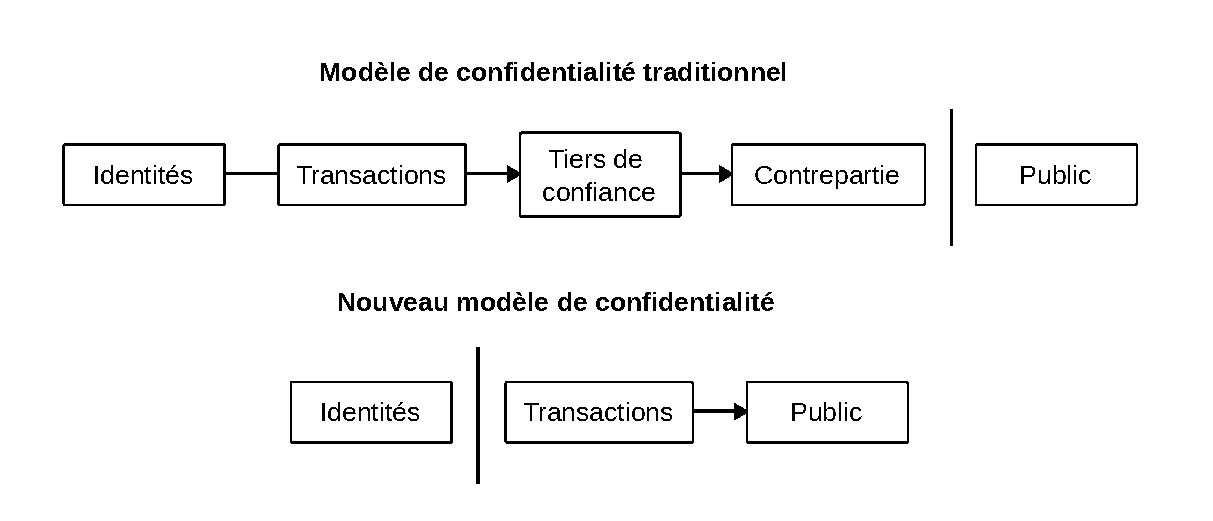
\includegraphics[scale=0.55]{img/white-paper-privacy-model-fr.eps}
  \caption{Modèle de confidentialité présenté dans le livre blanc de Bitcoin.}
\end{figure}

% Fuites d'information
Toutefois, des fuites d'information peuvent avoir lieu~: l'identité de l'utilisateur peut être dévoilée, que ce soit du fait de sa propre erreur ou de la divulgation (volontaire ou involontaire) de son interlocuteur dans l'échange. Par conséquent, nul ne peut prétendre être à l'abri de telles fuites\sendnote{Les premiers utilisateurs de Bitcoin ont ainsi été bien imprudents, à l'instar de Hal Finney qui a révélé des informations entre 2013 et 2014 permettant de déduire qu'il possédait plus de 10~000~bitcoins en 2011. -- Hal Finney, \emph{Bitcoin and me}, \wtime{19/03/2013 20:40:02 UTC}~: \url{https://bitcointalk.org/index.php?topic=155054.msg1643833\#msg1643833}~; Andy Greenberg, \eng{Nakamoto's Neighbor: My Hunt For Bitcoin's Creator Led To A Paralyzed Crypto Genius}, 25 mars 2014~: \url{https://www.forbes.com/sites/andygreenberg/2014/03/25/satoshi-nakamotos-neighbor-the-bitcoin-ghostwriter-who-wasnt/}.}. C'est pourquoi il existe des méthodes permettant de limiter leur effet et de retrouver la confidentialité en toute sérénité.

% Usage unique des adresses
La première mesure est l'usage unique des adresses. Elle consiste à générer une nouvelle clé privée et une nouvelle adresse lors de chaque paiement entrant et sortant. L'apport est de réduire l'impact de la révélation du lien avec l'identité sur la confidentialité générale~: tant que l'adresse n'est pas liée à d'autres par l'observation d'une action sur la chaîne (co-dépense par exemple), la fuite d'information se limite à cette seule adresse. Cette bonne pratique était citée dans le livre blanc\sendnote{«~Comme pare-feu supplémentaire, une nouvelle paire de clés devrait être utilisée pour chaque transaction afin de les empêcher d'être liées à un propriétaire commun. Certains liens sont toujours inévitables avec les transactions à entrées multiples, qui révèlent nécessairement que leurs entrées appartiennent au même propriétaire. Le risque est que si le propriétaire d'une clé est révélé, la liaison pourrait révéler d'autres transactions qui lui appartiennent.~» -- Satoshi Nakamoto, \eng{Bitcoin: A Peer-to-Peer Electronic Cash System}, 31 octobre 2008.} et est aujourd'hui implémentée dans tous les portefeuilles.

% Mélange de pièces
On peut également corriger les erreurs. Une des méthodes la plus connue pour procéder à ce type de correction est le mélange de pièces, qui permet de combiner ses UTXO avec d'autres utilisateurs afin de briser le lien déterministe qui existe.

% Tumblers
Le mélange de bitcoins était originellement pris en charge par des services de mixage centralisés, appelés \eng{mixers} ou \eng{tumblers}, qui recevaient les bitcoins des utilisateurs, les fusionnaient et leur renvoyaient des bitcoins communs au bout d'un certain temps, préférablement sous la forme de plusieurs transactions. Le premier mélangeur de ce type était BitLaundry, qui a été lancé en septembre 2010 par Peter Vessenes\sendnote{Peter Vessenes, \eng{Announcing: BitLaundry -- decorrelated payment service}, \wtime{01/09/2010 05:52:25 UTC}~: \url{https://bitcointalk.org/index.php?topic=963.msg11823\#msg11823}.}. Ces services permettaient d'obscurcir la provenance des bitcoins pour un observateur extérieur, mais pas pour le gérant du service, qui pouvait également voler les bitcoins au passage.  % Bitcoin Fog (2011), Silk Road

% CoinJoin
Une technique pour procéder à ce type de mélange sans devoir passer par un intermédiaire a par la suite été développée. C'était CoinJoin, dont la description formelle a été faite en août 2013 par Gregory Maxwell\sendnote{Gregory Maxwell, \eng{CoinJoin: Bitcoin privacy for the real world}, \wtime{22/08/2013 02:32:31 UTC}~: \url{https://bitcointalk.org/index.php?topic=279249.msg2983902\#msg2983902}.}. Il s'agit d'impliquer les pièces dans une transaction jointe collaborative qui brise la correspondance entre les entrées et une partie des sorties. La transaction classique que l'on se représente est celle de plusieurs utilisateurs qui signent chacun une entrée, dont la même nombre de sorties possèdent un montant égal, et dont le reste des sorties forment les sorties complémentaires. Dans ce cas, les sorties complémentaires sont toujours liées aux entrées, contrairement aux sorties principales qui sont indiscernables les unes des autres.

\textcolor{brown}{schéma transaction CoinJoin à 5 utilisateurs}

% Ensemble d'anonymat
Ces mélanges reposent sur la notion d'«~ensemble d'anonymat~» (\eng{anonymity set}) qui permet de mesurer la difficulté à faire le lien entre l'entrée et le sortie à un moment donné. On peut ainsi obtenir un score prospectif qui est le nombre de possibilités de pièces en sorties auxquelles peuvent correspondre un pièce en entrée. Dans notre exemple ci-dessus, le score prospectif de la sortie au moment de la transaction est de 5. Si la pièce avait subi un nouveau mélange (comme c'est fait dans Whirlpool), alors elle aurait eu un score prospectif de 9. On peut aussi, même si c'est plus rare, calculer un score rétrospectif qui correspond au nombre de potentielles pièces en entrée auxquelles peut être liée une sortie particulière, qui est également de 5 dans le cas de notre transaction simple, mais qui peut être largement supérieur en cas de remélanges fréquents. \sendnote{Loïc Morel, \emph{Comprendre et utiliser le CoinJoin sur Bitcoin}, 19 juillet 2022~: \url{https://www.pandul.fr/post/comprendre-et-utiliser-le-coinjoin-sur-bitcoin}.}

% Coordinateur
Pour gérer le tout, le système fait utilise généralement un protocole qui permet aux participants d'être mis en relation anonymement par le biais d'un coordinateur sans risque de fuite d'information ou de vol des fonds. Le plus connu est ZeroLink, développé par Adam Ficsor (\texttt{nopara73}) et \texttt{TDevD} en août 2017, qui est un protocole qui utilise le procédé de signature aveugle de David Chaum\sendnote{nopara73, TDevD, \eng{ZeroLink: The Bitcoin Fungibility Framework}, 14 août 2017~: \url{https://github.com/nopara73/ZeroLink/tree/32ad53927a343383534bea28fffb098af65fe62a}.}. C'est dans ce sens qu'on parle parfois de CoinJoin chaumien (\eng{Chaumian CoinJoin}). Une implémentation classique de cette idée a été réalisée par Whirlpool et par Wasabi 1.0. Des variantes (CoinShuffle, CoinShuffle++, CashShuffle, CashFusion) ont été implémentées sur des variantes de Bitcoin comme Decred ou Bitcoin Cash. Plus récemment le portefeuille Wasabi a intégré Wabisabi qui permet de réaliser des mélanges avec des valeurs arbitraires en sortie, ce qui complique l'estimation de la confidentialité apportée mais mais évite d'avoir à gérer les sorties complémentaires d'une manière séparée.

% PayJoin
Mais les transactions collaboratives ne se limitent pas au CoinJoin. Il existe par exemple une autre méthode, appelée PayJoin, qui permet de réaliser au commerçant de réaliser un mélange avec le client au moment du paiement, en impliquant une pièce en entrée. Cela a pour effet de fausser l'analyse de chaîne en faisant croire à l'observateur extérieur qu'un seul utilisateur a réuni ses pièces en entrée.

Reprenons notre exemple d'Alice qui paie 7~mBTC à Bob en réunissant deux pièces de 6 et 1~mBTC afin d'atteindre un montant suffisant en entrée. Dans ce cas, les deux entrées sont supposément liées entre elles (heuristique de co-dépense) ainsi qu'à la sortie de 1~mBTC (heuristique de la sortie complémentaire). Dans ce cas, PayJoin consiste à faire en sorte que le commerçant inclue une ou plusieurs pièces en entrée et augmente d'autant le montant de la sortie qui lui est destinée.

\textcolor{brown}{schéma transaction à 3 entrées et 2 sorties}

Cette technique a été conceptualisée en 2018 sous la forme du protocole Bustapay proposé dans le BIP-79, qui n'a été mis en application. Elle a est néanmoins implémentée aujourd'hui par l'intermédiaire du protocole de paiement Pay-to-EndPoint (P2EP) implémenté dans plusieurs portefeuilles\sendnote{Adam Ficsor, \eng{Pay To EndPoint}, 31 juillet 2018~: \url{https://nopara73.medium.com/pay-to-endpoint-56eb05d3cac6}.} et des transactions Stowaway du Samourai Wallet\sendnote{Samourai Wallet, \eng{Stowaway}~: https://samouraiwallet.com/stowaway}.

% CoinSwap
Enfin une dernière méthode est Coinswap, qui est un procédé développé par Chris Belcher, qui permet à deux utilisateurs ou plus d'échanger leurs pièces sans qu'ils aient besoin de se faire confiance et sans que cette opération laisse une trace particulière sur la chaîne\sendnote{Chris Belcher, \eng{Design for a CoinSwap Implementation for Massively Improving Bitcoin Privacy and Fungibility}, 25 mai 2020~: \url{https://gist.github.com/chris-belcher/9144bd57a91c194e332fb5ca371d0964}.}.

\section*{La machine virtuelle}
\addcontentsline{toc}{section}{La machine virtuelle}

% Monnaie programmable
Les scripts présents au sein des transactions font de Bitcoin un système de monnaie programmable. Ces scripts permettent en effet la mise en place d'une variété de conditions de dépense, aussi appelées clauses, qui vont au-delà de l'exigence d'une signature simple, comme la connaissance d'un secret, l'attente d'une période de temps ou la production de signatures multiples.

% Machine abstraite répliquée, machine virtuelle, machine à états
La mise en œuvre de Bitcoin crée une machine abstraite dont le fonctionnement est répliqué sur tous les nœuds du réseau grâce à l'algorithme de consensus. Elle est simulée par l'intermédiaire de l'implémentation logicielle, de sorte qu'on parle de machine virtuelle. Plus précisément, il s'agit d'un machine à états, dont l'état courant est l'ensemble des pièces existantes, c'est-à-dire l'ensemble des sorties transactionnelles non dépensées (UTXO), et dont les transitions sont les transactions, qui détruisent des pièces pour en créer de nouvelles. Ces transactions sont assemblées dans des blocs qui sont validés à intervalles réguliers par les mineurs. La diffusion d'un bloc sur le réseau permet d'actualiser l'état de la machine virtuelle, qui est la plupart du temps partagé par tous les nœuds.

% réplication de machine à états (\eng{state machine replication})
% FAUX : automate fini (appelé \eng{finite-state machine} en anglais) qui peut être dans une quantité finie d'états, mais qui n'est, à un moment donné, que dans un seul état\sendnote{Contrairement à ce qui est parfois affirmé, la machine virtuelle n'est pas un automate à deux piles (\eng{dual-stack pushdown automaton}), même si le langage de programmation interne en émule un. -- Craig S. Wright, \eng{Beyond Godel}, 2018~: \url{https://coingeek.com/wp-content/uploads/2018/03/SSRN-id3147440.pdf}.}. Même s'il est très grand, l'ensemble des états possibles est nécessairement fini en raison du codage des entiers sur 8 octets et de la limite de taille des scripts\sendnote{La limite de taille des scripts est actuellement de 10~ko sur BTC~: \url{https://github.com/bitcoin/bitcoin/blob/v0.17.0/src/script/script.h\#L31-L32}.}.

% Exécution des scripts
Au sein d'une transaction, le déverrouillage des pièces se fait par l'exécution de scripts. Les scripts sont des prédicats au sens mathématique, c'est-à-dire des expressions incomplètes qui deviennent des propositions pouvant être évaluées si elles sont complétées par un ou plusieurs éléments. De ce fait, la dépense consiste à réunir le script de verrouillage de la sortie précédente et le script de déverrouillage, et à les exécuter l'un après l'autre~: le script de déverrouillage d'abord, le script de verrouillage ensuite. L'utilisation de la pièce comme entrée de transaction n'est approuvée que si l'exécution réussit.

% Langage de programmation (règles de transition)
Les scripts sont écrits dans le langage de programmation interne de Bitcoin, conçu par Satoshi Nakamoto dès 2008 et baptisé de façon peu originale «~Script~». Ce langage de programmation fonctionne de manière similaire à Forth, un langage utilisé dans les années 1970 et 1980. Il se base en particulier sur deux piles de données, qui sont des structures de données fondées sur le principe du «~dernier arrivé, premier sorti~» (de l'anglais \eng{last in, first out}, abrégé en LIFO). Le langage agit essentiellement sur la pile primaire, de sorte que cette dernière est la plus importante~; la pile secondaire permet seulement de mettre des données de côté pendant l'exécution d'un script.

% Description par Satoshi
Satoshi Nakamoto a inclus ce système de scripts dans Bitcoin pour lui permettre de gérer une grande variété de cas d'utilisation. En juin 2010, en réponse à Gavin Andresen, il écrivait ainsi sur le forum~:

\begin{quote}
«~La nature de Bitcoin est telle que, dès la version 0.1 lancée, son fonctionnement de base était gravé dans le marbre pour le reste de son existence. C'est pour cette raison que je voulais concevoir Bitcoin pour qu'il supporte tous les types de transaction auxquels je pouvais penser. Le problème était que chaque élément requérait un code de prise en charge et des champs de données spéciaux, qu'il soit utilisé ou non, et ne pouvait couvrir qu'un cas particulier à la fois. Ç'aurait été une explosion de cas particuliers. La solution était script, qui généralisait le problème de façon à ce que les parties contractantes puissent décrire leurs transactions comme des prédicats que les nœuds du réseau évaluaient. Les nœuds ont seulement besoin de comprendre la transaction dans la mesure où ils évaluent si les conditions de l'émetteur sont remplies ou non.\sendnote{Satoshi Nakamoto, \eng{Re: Transactions and Scripts: DUP HASH160 ... EQUALVERIFY CHECKSIG}, \wtime{17/06/2010 18:46:08}~: \url{https://bitcointalk.org/index.php?topic=195.msg1611\#msg1611}.}~»
\end{quote} % "The nature of Bitcoin is such that once version 0.1 was released, the core design was set in stone for the rest of its lifetime.  Because of that, I wanted to design it to support every possible transaction type I could think of.  The problem was, each thing required special support code and data fields whether it was used or not, and only covered one special case at a time.  It would have been an explosion of special cases.  The solution was script, which generalizes the problem so transacting parties can describe their transaction as a predicate that the node network evaluates.  The nodes only need to understand the transaction to the extent of evaluating whether the sender's conditions are met."

% Opérateurs
Le langage est constitué de plus d'une centaine d'opérateurs, aussi appelés codes opération (ou \eng{opcodes} en anglais), qui agissent sur la pile primaire d'une manière ou d'une autre\sendnote{La liste des opérateurs et de leurs actions est disponible sur la page de Bitcoin Wiki consacrée à Script~: \url{https://en.bitcoin.it/wiki/Script}.}. Les opérateurs sont des nombres codés sur 1 octet (allant de 0 à 255), mais sont usuellement désignés par un nom décrivant leur fonction, dans le but de rendre la lecture plus compréhensible par l'être humain. Ils sont notés en majuscules et sont souvent précédés du préfixe \texttt{OP\_} même s'il peut être omis en l'absence d'ambiguïté. Par exemple, l'opérateur permettant de vérifier une signature (\texttt{0xac}) est noté \texttt{OP\_CHECKSIG} ou \texttt{CHECKSIG}.

% Empilement
Les opérateurs allant de 1 à 75, parfois notés \texttt{OP\_PUSHBYTES\_X}, ont pour action d'empiler des données ayant une taille allant de 1 à 75 octets. L'utilisation d'opérateurs supplémentaires spécifiques (notés \texttt{OP\_PUSHDATA\_Y}) permet cependant de placer une information plus grande sur la pile. Bien qu'on puisse utiliser cette notation, il est généralement plus simple de placer un élément entre chevrons pour indiquer qu'il est placé au sommet de la pile. Par exemple, le fait d'écrire \texttt{<signature>} au sein d'un script signifie que la signature est empilée.

% Valeur retournée
La valeur retournée à la fin de l'exécution des scripts est un booléen, de sorte que le script peut être valide, auquel cas la dépense de la pièce est approuvée, ou bien invalide, auquel cas la transaction est rejetée dans son ensemble. Le script est valide si et seulement si la valeur \texttt{TRUE} («~vrai~» en anglais) est présente en haut de la pile à la fin de l'exécution. Il est invalide si ce n'est pas le cas ou si son exécution s'est arrêtée avant la fin.

% Pas de boucles
Le langage Script est cependant limité. Rien dans sa conception ne permet pas de faire de boucles, ni d'accéder à des données extérieures à celles de la transaction, contrairement au langage d'Ethereum qui est quasi Turing-complet. Cette particularité fait qu'il est moins flexible, mais qu'il a l'avantage d'être plus simple à appréhender et donc plus sûr.

% Exemple : vérification d'une addition (38 = 17 + x)
L'exemple typique de script, présenté par Andreas Antonopoulos\sendnote{Andreas Antonopoulos, \eng{Mastering Bitcoin (second edition)}, ch.6, 2017.}, est celui qui consiste à résoudre une équation simple impliquant une addition. Si on considère l'équation $17 + x = 38$, alors le script de verrouillage qui correspond est~:

\begin{Verbatim}[fontsize=\small]
<17> ADD <38> EQUAL
\end{Verbatim}

Toute personne disposant de la réponse peut dépenser la pièce, ce qui on en convient n'est pas très sécurisé. La dépense requiert ici de fournir le script de déverrouillage composé uniquement de la solution de l'équation, à savoir 21~:

\begin{Verbatim}[fontsize=\small]
<21>
\end{Verbatim}

L'exécution successive de ces deux scripts a lieu comme suit~: 1)~la valeur 17 est placée sur la pile~; 2)~la valeur 21 est placée au-dessus~; 3)~l'opérateur \texttt{OP\_ADD} additionne les deux valeurs en haut de la pile et les remplace par leur somme, ici 38~; 4)~la valeur 38 est placée au sommet de la pile~; 5)~l'opérateur \texttt{OP\_EQUAL} compare les deux valeurs en haut de la pile et les remplace par le booléen d'égalité, ici \texttt{TRUE}. L'exécution du script est donc un succès.

\textcolor{brown}{schéma exécution du script et données sur la pile}

Si la valeur avait été différente, 22 par exemple, alors la dernière opération aurait retourné le booléen \texttt{FALSE} et la transaction de dépense aurait été invalidée.

% --- Exemples de scripts complets ---

Beaucoup de conditions de dépense différentes peuvent être implémentées par ce système. Certaines de ces conditions sont simples comme la connaissance d'un secret spécifique ou la production d'une signature valide correspondant à une clé publique particulière.

La connaissance d'un secret (dont l'empreinte est spécifiée dans l'UTXO) est vérifiée par les scripts suivants qui placent le secret au sommet de la pile, le hachent par SHA-256 et comparent le résultat à l'empreinte~:

\begin{Verbatim}[fontsize=\small]
<secret> || SHA256 <empreinte> EQUAL
\end{Verbatim}

De même, la vérification de la validité d'une signature est réalisée par les scripts suivants qui empilent d'abord la signature, puis la clé publique avant de contrôler leur correspondance~:

\begin{Verbatim}[fontsize=\small]
<signature> || <clé publique> CHECKSIG
\end{Verbatim}

% Verrous temporels
Mais il existe des conditions plus avancées comme les verrous temporels. Ceux-ci permettent de bloquer les fonds de la pièce pour un temps précis, que ce soit jusqu'à une date donnée, auquel cas on parle de temps de verrouillage absolu, ou bien pendant une période donnée, auquel cas on parle de temps de verrouillage relatif. Le premier est le fait de l'opérateur \texttt{OP\_CHECKLOCKTIMEVERIFY} dont les spécificités techniques sont décrites dans le BIP-65. Le second est appliqué par le code opération \texttt{OP\_CHECKSEQUENCEVERIFY} décrit dans le BIP-112.

% DESCRIPTION TECHNIQUE
%
% Les scripts suivants vérifient un temps de verrouillage absolu, c'est-à-dire lié à une date particulière~:
%
% \begin{verbatim}
% TRUE || <date de verrouillage> CHECKLOCKTIMEVERIFY DROP
% \end{verbatim}
%
% Le booléen \verb?TRUE? est mise en haut de la pile. Puis, est empilée la date jusqu'à laquelle le verrouillage persiste, qui est donnée en horodatage MTP ou en hauteur de blocs. Ensuite, cette date est comparée à la date indiquée dans le champ \verb?nLocktime? de la transaction, qui est elle-même comparée à l'horodatage du réseau. Enfin, la date est expulsée de la pile, ce qui fait qu'il ne reste que le booléen \verb?TRUE? sur la pile.
%
% Les scripts suivants vérifient un verrou temporel relatif, qui est lié à la période de temps écoulée depuis la date de confirmation de la pièce~:
%
% \begin{verbatim}
% TRUE || <période de verrouillage> CHECKSEQUENCEVERIFY DROP
% \end{verbatim}
%
% Le booléen \verb?TRUE? est mise en haut de la pile. Puis, c'est au tour de la période de verrouillage, qui est donnée en secondes\sendnote{Ou plus précisément en unités de 512 secondes.} ou en nombre de blocs. Ensuite, cette période est comparée à la période de temps indiquée dans le champ \verb?nSequence? de l'entrée dépensant la pièce, qui est elle-même comparée à la période de temps écoulée depuis la date de confirmation de la pièce. Enfin, la période est expulsée de la pile, ne laissant que le booléen \verb?TRUE? au sommet de la pile.
%
% Ce fonctionnement un peu plus compliqué des verrous temporels s'explique par le fait qu'ils ont été intégrés sous la forme de soft fork.


\section*{Les schémas classiques}
\addcontentsline{toc}{section}{Les schémas classiques}

% --- Schémas et règles de mempool ---

Le langage Script permet de faire des choses diverses et variées. Pendant les premiers temps de Bitcoin, le système était relativement libre et autorisait les gens à écrire ce qu'ils voulaient dans les scripts sans discrimination. Toutefois, cette situation était considérablement risquée. La raison principale était que le fonctionnement des codes opération n'était pas encore vérifié et testé, comme l'a montré la découverte en juillet 2010 d'une vulnérabilité rendue possible par certains opérateurs binaires\sendnote{NIST, \eng{CVE-2010-5137}, 8 juin 2012~: \url{https://nvd.nist.gov/vuln/detail/CVE-2010-5137}.}. C'est pourquoi il a été décidé à la fin de l'année 2010, sous l'impulsion de Gavin Andresen, de restreindre la facilité de programmation du système\sendnote{Gavin Andresen, \eng{svn r197: IsStandard check for transactions}, \wtime{07/12/2010 13:58:33 UTC}~: \url{https://bitcointalk.org/index.php?topic=2129.msg27744\#msg27744}.}.

% Schémas standards
Cette restriction a été appliquée en imposant des schémas standards de scripts, qui faisaient que les nœuds configurés par défaut ne relayaient plus les transactions contenant des scripts qui ne respectaient pas ce standard. Il ne s'agissait pas ainsi d'une restriction des règles globales de consensus, mais des règles locales de mempool qui s'applique à la transmission des transactions. Des schémas standards rendant les choses plus simples et plus sûres ont ainsi été développés au cours des années. Les schémas standards de sortie transactionnelle étaient \textcolor{darkgray}{en 2023} au nombre de huit~: P2PK, P2PKH, P2MS, P2SH, NULLDATA, P2WPKH, P2WSH et P2TR\sendnote{\url{https://github.com/bitcoin/bitcoin/blob/22.x/src/script/standard.h\#L59-L71}.}.

% --- Pay to Public Key ---

\textbf{P2PK~: Pay to Public Key} Le premier schéma s'appelle Pay to Public Key (P2PK), qu'on peut traduire littéralement en français par «~payer à la clé publique~». Il s'agit de créer une pièce liée à la clé publique d'un destinataire, que lui seul peut dépenser en signant avec sa clé privée. Le script de verrouillage permettant ce type d'envoi est~:

\begin{Verbatim}[fontsize=\small]
<clé publique> CHECKSIG
\end{Verbatim}

La présence de la clé publique explique qu'on parle parfois de «~scriptPubKey~» pour désigner le script de verrouillage en général, indépendemment de ce qu'il contient.

Au moment de la dépense, le destinataire doit utiliser un script de déverrouillage contenant simplement sa signature~:

\begin{Verbatim}[fontsize=\small]
<signature>
\end{Verbatim}

La présence de la signature dans ce script explique qu'on parle parfois de «~scriptSig~» pour désigner le script de déverrouillage en général, indépendemment de ce qu'il contient.

L'exécution successive de ces deux scripts permet, comme on l'a vu, de vérifier que la signature fournie par l'utilisateur correspond à sa clé publique, auquel cas elle est valide.

Le schéma P2PK était utilisé dans les débuts de Bitcoin pour recevoir les paiements par IP (P2IP) et pour récupérer la récompense de minage. Il est aujourd'hui tombé en désuétude au profit d'un schéma rival~: P2PKH.

% --- Pay to Public Key Hash --

\textbf{P2PKH~: Pay to Public Key Hash.} Le schéma Pay to Public Key Hash (P2PKH), qui est traduit littéralement par «~payer à l'empreinte de la clé publique~», est le deuxième type de format de réception apparu dans Bitcoin dès le début du fait de la conception de Satoshi Nakamoto. Ce schéma permet non pas de réaliser un paiement vers une clé publique, mais vers l'empreinte d'une clé publique, tout en faisant en sorte que l'interpréteur vérifie quand même la validité de la signature vis-à-vis de la clé publique lors de la dépense des fonds. L'empreinte de la clé publique est alors considérée comme la donnée essentielle de l'adresse, qui dans ce cas commence toujours par un 1, comme par exemple \longstring{1FjBKPQ7MTiPSDkJ2ZwPgAXUKQ8yoGbVJX}.

Le script de verrouillage ici est~:

\begin{Verbatim}[fontsize=\small]
DUP HASH160 <empreinte de la clé publique> EQUALVERIFY CHECKSIG
\end{Verbatim}

Et le script de déverrouillage est~:

\begin{Verbatim}[fontsize=\small]
<signature> <clé publique>
\end{Verbatim}

L'exécution des deux scripts permet de~: 1) vérifier que le passage de la clé publique par la fonction de hachage HASH-160 est égale à l'empreinte qui est spécifiée dans le script ; 2) vérifier la signature correspond à la clé publique.

L'avantage de ce schéma est qu'il permet d'avoir des adresses plus courtes (l'information à encoder n'est que de 20~octets au lieu de 65~octets pour une clé publique), raison pour laquelle Satoshi Nakamoto l'a implémenté. De plus, en ne révélant la clé publique qu'au moment de la dépense, ce schéma accroît aussi la sécurité contre la menace (très hypothétique) de l'ordinateur quantique.

% --- Pay To MultiSig ---

\textbf{P2MS~: Pay To MultiSig.} Le schéma Pay To MultiSig (P2SH), qui signifie littéralement «~payer à la multisignature~», est un schéma exigeant la signature de M personnes parmi N participants prédéterminés («~M-parmi-N~», ou «~M-of-N~» en anglais). Il a été rendu standard sous une forme limitée à 3 participants en mars 2012 avec la sortie de la version 0.6.0 du logiciel\sendnote{Gavin Andresen, \eng{Version 0.6.0 released}, 30 mars 2012~: \url{https://bitcointalk.org/index.php?topic=74737.msg827484\#msg827484}.}. Le script de verrouillage est le suivant~:

\begin{Verbatim}[fontsize=\small]
M <clé publique 1> ... <clé publique N> N CHECKMULTISIG
\end{Verbatim}

Le script de déverrouillage correspondant est~:

\begin{Verbatim}[fontsize=\small]
<leurre (0)> <signature 1> ... <signature M>
\end{Verbatim}

La présence du leurre (généralement 0) est dû à un défaut dans l'implémentation de l'exécution de l'opérateur \texttt{OP\_CHECKMULTISIG} par Satoshi, qui requiert un élément de trop. Les développeurs n'ont pas jugé rentable de corriger ce défaut, car cette correction constituait un hard fork.

C'est ce schéma, particulièrement exigeant au niveau de la mise en place, qui a motivé la création du schéma P2SH.

\textbf{P2SH : Pay to Script Hash} Le schéma Pay to Script Hash (P2SH), pouvant être traduit littéralement par «~payer à l'empreinte du script~», reprend l'idée derrière P2PKH, à la seule différence que la donnée hachée n'est pas une clé publique, mais le script lui-même~! Le script en question est alors appelé script de récupération (\eng{redeem script}) pour le différencier du script de déverrouillage. Son empreinte est la donnée constituante de l'adresse, cette dernière commençant toujours par un 3 à l'instar de \longstring{3K8Ps6Ayw5ZaKDaLZjfGo3mTgDsc1VXZ8d}.

% \sendnote{Ludovic Lars, \emph{Pay to Script Hash (P2SH) pleinement expliqué}, 14 juillet 2020~: \url{https://viresinnumeris.fr/pay-to-script-hash-p2sh-pleinement-explique/}.}

Ce schéma donne à l'utilisateur la possibilité d'y inclure n'importe quel script, sans discrimination sur son format, à condition qu'il respecte bien sûr certaines limites. Il permet aussi de recevoir des fonds depuis la quasi-totalité des portefeuilles existants, le fardeau de la construction et du déverrouillage du script revenant uniquement au destinataire, et pas aussi à l'expéditeur comme c'est le cas dans le scripting brut.

Le script de verrouillage pour le schéma P2SH est~:

\begin{Verbatim}[fontsize=\small]
HASH160 <empreinte du script de récupération> EQUAL
\end{Verbatim}

Et le script de déverrouillage est un script de la forme~:

\begin{Verbatim}[fontsize=\small]
[éléments de déverrouillage] <script de récupération>
\end{Verbatim}

L'exécution de P2SH est plus complexe que les précédents schémas, ce qui peut s'expliquer par le contexte dans lequel il a été développé. L'idée d'implémenter un schéma de script qui utilise l'empreinte d'un autre script comme l'empreinte de clé publique dans le schéma P2PKH est née 2011 en faisant l'objet de plusieurs propositions\sendnote{Mike Caldwell (casascius), \eng{Proposal to modify OP\_CHECKSIG}, \wtime{22/09/2011 02:21:17 UTC}~: \url{https://bitcointalk.org/index.php?topic=45211.msg538756\#msg538756}~; jimrandomh, \eng{Proposed extensions to the transaction protocol: Receiver scripts, OP\_TIME, more}, \wtime{01/10/2011 16:56:47 UTC}~: \url{https://bitcointalk.org/index.php?topic=46429.msg553217\#msg553217}~; Gavin Andresen, \eng{Re: Proposal to modify OP\_CHECKSIG}, \wtime{02/10/2011 00:26:42 UTC}~: \url{https://bitcointalk.org/index.php?topic=45211.msg553668\#msg553668}.}. Elle a été rendue plus concrète avec une proposition de l'opérateur \texttt{OP\_EVAL} par Nicolas van Saberhagen le 2 octobre, code opération qui permettait l'exécution récursive d'un script à l'intérieur d'un autre script\sendnote{Nicolas van Saberhagen, \eng{OP\_EVAL proposal}, \wtime{02/10/2011 00:49:19 UTC}~: \url{https://bitcointalk.org/index.php?topic=46538.msg553689\#msg553689}.}. Gavin Andresen a expliqué comment en faire un soft fork par le remplacement de l'instruction sans effet \texttt{OP\_NOP1}\sendnote{Gavin Andresen, \eng{Re: OP\_EVAL proposal}, \wtime{02/10/2011 20:42:32 UTC}~: \url{https://bitcointalk.org/index.php?topic=46538.msg554620\#msg554620}.}.

L'opérateur \texttt{OP\_EVAL} devait permettre de former un nouveau schéma standard. Le script de verrouillage aurait été~:

\begin{Verbatim}[fontsize=\small]
DUP HASH160 <empreinte du script de récupération> EQUALVERIFY EVAL
\end{Verbatim}

tandis que le script de déverrouillage aurait été le même. L'exécution successive de ces deux scripts aurait permis dans un premier temps de vérifier la conformité du hachage du script de récupération à l'empreinte~; puis dans un second temps d'exécuter le script de récupération et de lui combiner les éléments de déverrouillage.

Néanmoins cette solution n'a pas été acceptée, celle-ci ayant été jugée trop dangereuse à cause de son pouvoir de récursion. Il lui a été préféré le modèle plus restrictif de P2SH.

L'exécution de P2SH fonctionne exactement comme le schéma lié à \texttt{OP\_EVAL}, à l'exception qu'une partie du script n'est pas explicitement indiquée. D'une part, la vérification de la correspondance entre l'empreinte indiquée et le script de récupération est bien réalisée par le script de verrouillage. D'autre part, l'évaluation du script de récupération est effectuée implicitement grâce à une exception ajoutée au code source qui fait que les nœuds du réseau qui reconnaissent le schéma l'interprètent différemment. Dans Bitcoin Core, on peut observer cette condition au sein de la fonction \texttt{VerifyScript} de l'interpréteur\sendnote{\url{https://github.com/bitcoin/bitcoin/blob/22.x/src/script/interpreter.cpp\#L2018-L2062}}.

% Laideur
La proposition a été codifiée dans le BIP-16. Si cette solution est pratique, elle crée de la complexité et n'est pas très élégante. Comme le disait Gavin Andresen dans l'explication du BIP-16~:

\begin{quote}
«~Reconnaître une forme "spéciale" de scriptPubKey et réaliser une validation supplémentaire quand elle est détectée, c'est laid. Cependant, l'avis général est que les alternatives sont soit encore plus laides, soit plus complexes à implémenter, et/ou étendent le pouvoir du langage d'expression de manière dangereuse.\sendnote{Gavin Andresen, \eng{BIP-16: Pay to Script Hash}, 3 janvier 2012~: \url{https://github.com/bitcoin/bips/blob/master/bip-0016.mediawiki\#rationale}.}~»
\end{quote}

Le schéma P2SH a été activé le 1\ier{} avril 2012 sous la forme d'un soft fork, en dépit de l'opposition notable de luke-jr qui proposait un opérateur alternatif, \texttt{OP\_CHECKHASHVERIFY}, décrit dans le BIP-17\sendnote{Amir Taaki, \eng{The Truth behind BIP 16 and 17}, 29 janvier 2012~: \url{http://bitcoinmedia.com/the-truth-behind-bip-16-and-17/}~; archive~: \url{https://web.archive.org/web/20120202032835/http://bitcoinmedia.com/the-truth-behind-bip-16-and-17/}.}.

\section*{Les types de signature}
\addcontentsline{toc}{section}{Les types de signature}

% --- Types de signature ---

La programmabilité de Bitcoin n'est pas seulement issue de son langage de programmation mais aussi du système de signature qui permet de de sélectionner quelle partie de la transaction est signée. Ce facteur de programmabilité est mis en œuvre par l'existence d'un indicateur, appelé type de hachage de la signature ou \eng{signature hash type}, qui est ajouté à la transaction non signée, puis à la signature elle-même. Celui-ci indique quelle partie de la transaction doit être hachée avant d'être soumise à l'algorithme de signature, d'où son nom.

Le type de signature est construit à partir de plusieurs signaux de signature qui peuvent être combinés. Les quatre signaux de signature qui existent sont~:

\begin{itemize}
\item[$\bullet$] \texttt{SIGHASH\_ALL} (\texttt{0x01}) qui indique que toutes les sorties sont signées~;
\item[$\bullet$] \texttt{SIGHASH\_SINGLE} (\texttt{0x03}) qui permet de ne signer qu'une seule sortie~;
\item[$\bullet$] \texttt{SIGHASH\_NONE} (\texttt{0x02}) qui indique qu'aucune sortie n'est signée~;
\item[$\bullet$] \texttt{SIGHASH\_ANYONECANPAY} (\texttt{0x80}) qui permet de ne signer qu'une seule entrée.
\end{itemize}

Les trois signaux concernant les sorties peuvent être associés à \texttt{SIGHASH\_ANYONECANPAY}, ce qui permet de former finalement six types de signatures différents. Le type de signature le plus fréquent est évidemment \texttt{SIGHASH\_ALL} même si certains autres types peuvent parfois trouver une utilité. C'est notamment le cas de \texttt{SIGHASH\_ALL | SIGHASH\_ANYONECANPAY} qui permet de construire des transactions de type \eng{anyone-can-pay}, dont les sorties sont déterminées, mais où chacun peut signer sa propre entrée sans connaître les autres.

\textcolor{brown}{schéma types de signature}

% Notez que tout ceci était présent dès la création de Bitcoin et que Satoshi Nakamoto avait intégré ce type de signature dans le code d'origine.

% SIGHASH_NOINPUT
Ces signaux ont été implémentés dès le début par Satoshi Nakamoto au sein du prototype. Il en manquait logiquement un, que Satoshi Nakamoto a probablement jugé inutile~: celui qui ne signait aucune entrée. Toutefois, avec le développement des canaux de paiements pour le réseau Lightning, les développeurs se sont rendus compte qu'il pouvait avoir une utilité. C'est dans cet esprit que le signal de signature \texttt{SIGHASH\_NOINPUT} a été proposé en février 2016 par Joseph Poon\sendnote{Joseph Poon, \eng{[bitcoin-dev] SIGHASH\_NOINPUT in Segregated Witness}, \wtime{26/02/2016 01:07:46 UTC}~: \url{https://lists.linuxfoundation.org/pipermail/bitcoin-dev/2016-February/012460.html}.}.

% BIP-118, SIGHASH_ANYPREVOUT
Ce type de signal pourrait être implémenté de manière partielle dans BTC au travers du BIP-118, qui prévoit l'implémentation de deux nouveaux signaux -- \texttt{SIGHASH\_ANYPREVOUT} et \texttt{SIGHASH\_ANYPREVOUTANYSCRIPT} -- au sein des scripts de Taproot\sendnote{Christian Decker, Anthony Towns, \eng{BIP-118: SIGHASH\_ANYPREVOUT for Taproot Scripts}, 28 février 2017~: \url{https://github.com/bitcoin/bips/blob/master/bip-0118.mediawiki}.}. Il permettrait d'améliorer le fonctionnement du réseau Lightning par la mise en œuvre du protocole Eltoo qui repose sur la construction de transactions flottantes.

\section*{SegWit~: le témoin séparé}
\addcontentsline{toc}{section}{SegWit~: le témoin séparé}

% Présentation de SegWit
SegWit, abréviation de \eng{Segregated Witness}, qu'on peu traduire littéralement par «~témoin séparé~», est une mise à niveau du protocole ayant lieu sur LTC et sur BTC en 2017. Elle a consisté à faire en sorte que les données de déverrouillage des entrées transactionnelles, telles que les signatures, se retrouvent dans une structure de données séparée (\eng{segregated}) appelée le témoin (\eng{witness}) afin de supprimer la malléabilité des transactions. SegWit constituait ainsi une restructuration profonde des transactions.

% Autres apports
Outre la correction de la malléabilité, SegWit a apporté une augmentation de capacité transactionnelle et un versionnage des scripts pour faciliter les mises à niveau ultérieures. Elle a également amélioré l'algorithme de signature pour éviter les hachages redondants durant la vérification et pour rendre plus sûre la signature hors-ligne\sendnote{Voir BIP-143~: \url{https://github.com/bitcoin/bips/blob/master/bip-0143.mediawiki}.}.

% --- Malléabilité ---

\textbf{Malléabilité.} SegWit tire son origine du problème de la malléabilité des transactions, un problème qui est identifié depuis janvier 2012\sendnote{Gavin Andresen, \eng{[Bitcoin-development] Extending IsStandard() to transaction scriptSigs}, \wtime{19/1/2012 16:29:29}, \url{https://lists.linuxfoundation.org/pipermail/bitcoin-dev/2012-January/001066.html}.}. Dans Bitcoin, les transactions sont malléables dans le sens où elles peuvent être modifiées légèrement après leur diffusion sans devenir invalides aux yeux du réseau. Cette propriété vient du fait qu'une signature ne peut pas se prendre en compte elle-même et que par conséquent le script de déverrouillage n'est pas signé avec le reste de la transaction. La malléabilité peut ainsi prendre deux formes~: la malléabilité intrinsèque à l'algorithme ECDSA, qui se base sur un nombre aléatoire pour produire une signature (malléabilité par le signataire)~; la malléabilité provenant de la forme des signatures et des scripts de déverrouillage des entrées (malléabilité par un tiers).

% Problèmes
La malléabilité n'est pas rédhibitoire pour la sécurité des fonds, mais elle permet de modifier l'identifiant de la transaction après sa publication, ce qui peut se révéler problématique dans certaines situations. Ainsi, entre le 9 et le 11 février 2014, Mt. Gox et d'autres plateformes d'échange ont subi des attaques exploitant cette malléabilité des transactions\sendnote{Ken Shirriff, \eng{The Bitcoin malleability attack graphed hour by hour}, 15 février 2014~: \url{https://www.righto.com/2014/02/the-bitcoin-malleability-attack-hour-by.html}}. Les transactions de retrait ont été modifiées par les attaquants, faisant croire aux plateformes mal configurées que ces transactions n'avaient pas été confirmées, ce qui leur a permis de recréditer leur compte tout en conservant les bitcoins. Ces attaques ont mené à une perte totale de 64~564~bitcoins\sendnote{Christian Decker, Roger Wattenhofer, \eng{Bitcoin Transaction Malleability and MtGox}, 26 mars 2014~: \url{https://arxiv.org/pdf/1403.6676.pdf\#page=8}.}.

% Tentatives de correction
Des propositions ont tenté de corriger la malléabilité par un tiers en contraignant au maximum la forme des transactions. C'est dans cet esprit que le BIP-62 a été créé en mars 2014, dont l'une des exigences (l'encodage standard des signatures décrit dans le BIP-66) a été incluse dans les règles de consensus le 4 juillet 2015. Toutefois, ces changements ne s'appliquaient pas à la malléabilité par le signataire, ce qui créait la demande pour une correction généralisée.

% Lightning Network
Cette malléabilité signifiait que tout acteur participant à un schéma de multisignature pouvait modifier la transaction et donc son identifiant à tout moment. Cela altérait significativement la possibilité d'implémentation du réseau Lightning, dont les canaux de paiements, comme on le verra plus bas, se basent sur des transactions non publiées auxquelles il faut faire référence et font intervenir des signatures multiples.

% Solution : séparer les signatures du reste de la transaction
La solution était de mettre de côté les scripts de déverrouillage dans le processus de hachage de la transaction, pour qu'un changement de ces scripts n'influence pas l'identifiant. Cette idée a été proposée initialement par Gregory Maxwell en août 2013 sur IRC\sendnote{«~Je suggère de ne jamais hacher cette valeur dans le protocole. En gros, je dis que les scriptsigs pour une [transaction] seraient un arbre de hachage séparé. Il est toujours engagé dans la chaîne de blocs mais ce serait une branche séparée.~» -- Gregory Maxwell, IRC, \wtime{29/08/2013 20:21 UTC}~: \url{https://download.wpsoftware.net/bitcoin/wizards/2013/08/13-08-29.log}.}, avant d'être mise en œuvre au sein de la version alpha du modèle de sidechain appelé Elements, annoncée le 8 juin 2015 par Blockstream\sendnote{\url{https://blog.blockstream.com/en-714/}}. Le même jour, Gregory Maxwell présentait cette version d'Elements incluant \eng{Segregated Witness} dans un séminaire de développements de San Francisco~: il décrivait alors le témoin comme «~une valeur spécifique qui constitue une preuve concrète d'affirmation existentielle\sendnote{\url{https://www.youtube.com/watch?v=Twynh6xIKUc}~; \url{https://mirror.explodie.org/blockstream.gmaxwell.elements.talk.060815.pdf}.}~».

% 20:21 < gmaxwell> e.g. OP_NOP <push> checksig is still valid.. so you'd have to have a rule saying you couldn't do that.  But I'm suggesting never hashing that value anywhere in the protocol.
% 20:21 < gmaxwell> basically I'm saying the scriptsigs for a txn would be a seperate hashtree. You'd still commit it in the blockchain but it would be a seperate fork.

% SegWit en tant que proposition d'amélioration de Bitcoin
Cette solution a été adaptée pour Bitcoin au cours de l'automne 2015, pour être appliquée comme un soft fork. La mise à niveau SegWit a été officiellement introduite à la communauté par le développeur Pieter Wuille le 7 décembre 2015, lors de la conférence Scaling Bitcoin \textsc{II} à Hong Kong. En substance, elle consistait à déplacer les scripts de déverrouillage dans le témoin de la transaction. Deux identifiants étaient alors calculés~: l'identifiant classique (\texttt{txid}), qui ne prend pas en compte ce témoin, et l'identifiant complet (noté \texttt{wtxid} pour \eng{witness transaction identifier}), qui recouvre l'intégralité de la transaction. Les identifiants complets étaient regroupés dans un second arbre de Merkle, dont la racine était placée dans la transaction de récompense du bloc, ce qui faisait que toutes les données étaient engagées dans le calcul de la preuve de travail. De l'autre côté, les transactions et les blocs restaient valides pour les nœuds n'ayant pas été mis à niveau.

% Correction de la malléabilité
SegWit est active depuis le 24 août 2017. L'absence de script de déverrouillage dans le calcul de l'identifiant classique permet de ne plus avoir de malléabilité du tout, ni des signataires, ni d'un tiers extérieur.

% Augmentation de la capacité transactionnelle
\textbf{Augmentation de la capacité transactionnelle.} SegWit a aussi eu pour effet indirect de créer un bloc d'extension et d'augmenter la capacité transactionnelle. En effet, les nœuds suivant les anciennes règles ne voyaient pas le témoin, de sorte qu'ils ne le comptabilisaient pas dans la taille du bloc. La question était alors de savoir quelle limite mettre sur le témoin.

% Nouvelle métrique : le poids
La réponse a été d'inventer une nouvelle métrique pour mesurer l'impact des transactions et des blocs sur le réseau~: le poids, ou\eng{weight} en anglais, qui est une moyenne pondérée de la taille de base et de la taille du témoin. Exprimé en unités de poids (\eng{weight unit}), il est défini comme la somme du quadruple de la taille de base et de la taille du témoin~:

\[
w = 4 \cdot s_b + s_w
\]

% Taille virtuelle, poids limite des blocs
Il en découle une taille virtuelle qui est définie comme la somme de la taille de base et du quart de la taille du témoin, c'est-à-dire~: $s_v = s_b + \frac{s_w}{4}$. La taille limite des blocs est devenue un poids limite des blocs, qui était de 4 millions d'unités au moment de la mise à niveau et qui \textcolor{darkgray}{est toujours la même en 2023}.

% Calcul des frais
De ce fait, les frais qui étaient intialement calculés en satoshis par octet (sat/o), sont, depuis SegWit mesurés en satoshis par octet virtuel (sat/ov). Les mineurs sélectionnent les transactions en fonction de ce taux afin d'être les plus rentables possibles par rapport à cette limite. Cet effet n'est valable que si la limite est atteinte.

% Meilleure pondération par rapport à l'ensemble des UTXO
Avec SegWit, il s'agissait donc de pondérer l'impact des entrées par rapport à celle des sorties sur le calcul des frais. Si la limite de capacité était atteinte, alors les sorties étaient quatre fois plus chères à inscrire sur la chaîne que les scripts de déverrouillage contenus dans les entrées. La mise à niveau, en plus d'installer une remise qui incite à son usage, a créé une dissuasion à alourdir l'ensemble des UTXO. Le facteur 4 se rapprochait de la pondération matérielle\sendnote{SegWit Resources, \eng{Why a discount factor of 4? Why not 2 or 8?}, 13 janvier 2017~: \url{https://medium.com/segwit-co/why-a-discount-factor-of-4-why-not-2-or-8-bbcebe91721e}.}.

% Taille réelle des blocs
Cette limite de 4 millions d'unités de poids est indicative. La taille réelle des blocs n'atteint généralement pas 4~Mo en raison de la forme des transactions. Les données contenues dans une transaction normale ne sont en effet pas regroupées dans le témoin, de sorte qu'elle ne remplissent pas entièrement l'espace de bloc autorisé. Par exemple, si nous prenons un bloc constitué uniquement de transactions à 2 entrées et 2 sorties utilisant SegWit, alors sa taille réelle sera de 1,784~Mo\sendnote{Une transaction à 2 entrées et 2 sorties de type P2WPKH mesure 372~o et pèse 834~wu au maximum. De ce fait, il est possible d'inclure 4796~transactions dans un bloc, ce qui nous permet de calculer sa taille réelle.}.

% Avantage donné aux grands témoins
Les transactions dont les données de déverrouillage sont plus grandes profitent mieux de cet espace de bloc supplémentaire. C'est le cas des transactions utilisant la multisignature comme les fermetures de canaux de paiement. Il est ainsi possible d'approcher la taille des 4~Mo en maximisant la taille des données contenues dans le témoin. C'est ce qui a été fait le 1\ier{} février 2023 avec la création d'un bloc de 3,955~Mo dont le témoin a servi à l'inscription d'une image\sendnote{Voir le bloc 774~628, d'identifiant \longstring{0000000000000000000515e202c8ae73c8155fc472422d7593af87aa74f2cf3d} dont la taille était de 3~955~272~octets et qui incluait une transaction qui mesurait à elle seule 3~938~383~octets.}

% --- Versionnage des scripts ---

\textbf{Versionnage des scripts.} Enfin, la mise à niveau SegWit a apporté un versionnage des scripts, qui permettait le déploiement de futures mises à niveau. La version permettait ainsi d'indiquer quelles règles étaient appliquées. La première version de SegWit en 2017 utilisait la version 0, et le déploiement de Taproot en 2021 a été fait au travers de la version 1.

% --- Types de sortie ---

Trois types de sortie existent pour l'instant~: le schéma P2WPKH, le schéma P2WSH et le schéma P2TR.

\textbf{P2WPKH~: Pay to Witness Public Key Hash.} Le schéma \eng{Pay to Witness Public Key Hash} (P2WPKH), qui signifie littéralement «~payer à l'empreinte de la clé publique témoin~», est le premier schéma mis en place par SegWit. L'empreinte de la clé publique est obtenue par le hachage standard (SHA-256 + RIPEMD-160). Le script de verrouillage apparent est alors~:

\begin{Verbatim}[fontsize=\small]
<version (0)> <empreinte (hash160) de la clé publique>
\end{Verbatim}

Ce script est \eng{anyone-can-spend}. Le type de la sortie est détecté par l'interpréteur grâce à sa forme~: la version de SegWit (ici 0) et la taille de l'empreinte (ici 20 octets). La version et l'empreinte forment l'information essentielle de l'adresse, qui est encodée grâce au format Bech32 et qui commence toujours par \texttt{bc1q}, à l'instar de \longstring{bc1q5x9a0aqmgtrucm4l5n0y8e4kxfy9xm4udhygr2}.

Le script de déverrouillage est vide. Les données de déverrouillage sont contenues dans le témoin de la transaction. La partie du témoin correspondant à l'entrée est~:

\begin{Verbatim}[fontsize=\small]
<2> <signature> <clé publique>
\end{Verbatim}

\textbf{P2WSH~: Pay to Witness Script Hash} Le schéma \eng{Pay to Witness Script Hash} (P2WSH), dont la traduction littérale est «~payer à l'empreinte du script témoin~», est la retranscription de P2SH pour SegWit.

L'empreinte du script de récupération est obtenue par SHA-256, par peur d'une collision de RIPEMD-160 dans le cas d'une adresse générée par plusieurs personnes\sendnote{Gavin Andresen, \eng{[bitcoin-dev] Time to worry about 80-bit collision attacks or not?}, \wtime{07/01/2016 19:02:05 UTC}~: \url{https://lists.linuxfoundation.org/pipermail/bitcoin-dev/2016-January/012198.html}.}. le script de verrouillage est le suivant~:

\begin{Verbatim}[fontsize=\small]
<version (0)> <empreinte (sha256) du script de récupération>
\end{Verbatim}

Ce script est encore une fois \eng{anyone-can-spend} de manière apparente. Le type de la sortie est détecté par l'interpréteur grâce à sa forme~: la version de SegWit (ici 0) et la taille de l'empreinte (ici 32 octets). L'adresse est encore une fois constituée de ces deux informations et encodée grâce au format Bech32.

Le script de déverrouillage est vide. Les données de déverrouillage sont contenues dans le témoin de la transaction. La partie du témoin correspondant à l'entrée est~:

\begin{Verbatim}[fontsize=\small]
<nombre d'élements + 1> [éléments de déverrouillage] <script de récupération>
\end{Verbatim}

Dans les deux cas, l'empreinte est aussi appelée «~programme du témoin~».

\textbf{Types imbriqués (P2SH-P2WPKH, P2SH-P2WSH)} SegWit a aussi modifié le format P2SH pour inclure de nouvelles exceptions. Ces exceptions correspondent aux types imbriqués P2SH-P2WPKH et P2SH-P2WSH. Leur fonctionnement consiste à inclure les scripts de verrouillages précédents (version + empreinte) dans une sortie P2SH en tant que scripts de récupération. Le script de récupération est alors exécuté différemment pour faire appel aux données contenues dans le témoin.

Ces types imbriqués facilitaient la transition vers SegWit en permettant aux portefeuilles non mis à jour d'envoyer des fonds vers des adresses SegWit. L'utilisation d'adresses SegWit natives restait néanmoins plus avantageuse.

\textbf{P2TR~: Pay to Taproot} Le dernier schéma à rentrer en vigueur est le schéma \eng{Pay to Taproot} (P2TR), ce qui peut être traduit par «~payer à Taproot~». Ce schéma permet de recevoir un paiement sur une clé publique externe qui cache une clé privée ou bien la racine pivot d'un arbre syntaxique abstrait merkélisé (ou MAST pour \eng{Merklized Abstract Syntax Trees}) contenant les clauses d'un contrat autonome. Le paiement se fait vers une clé publique~: c'est donc un retour vers le P2PK. Cette clé publique externe cache une clé privée servant à signer les fonds, ou bien la racine pivot d'un arbre syntaxique abstrait merkélisé (ou MAST pour \eng{Merklized Abstract Syntax Trees}) contenant les clauses d'un contrat autonome. Le script de verrouillage présent dans la sortie transactionnelle est~:

\begin{Verbatim}[fontsize=\small]
<version (1)> <clé publique Taproot>
\end{Verbatim}

La clé publique en question mesure 32 octets. La version et la clé publique constituent les éléments constitutifs de l'adresse, qui est encodée grâce au format Bech32m et qui commence par \texttt{bc1p} comme par exemple \longstring{bc1pqlqqhzrg60v5h87r8lugusrddgz0j306shcupthy0tdqaqurwn8qr8qsej}. Le déverrouillage de la sortie se fait avec une signature simple, ou bien avec l'exécution du MAST.

% tr(f6a6c7c39c88b767bfac4ac687c3ff32372e76c9fb633e2278e54472e300b3bd)

% --- Conclusion et défauts ---

SegWit a donc modifié en profondeur le protocole. La forme de cette mise à niveau ne peut être comprise que dans le contexte dans lequel elle a émergé. C'est pourquoi elle présente tout de même quelques défauts comme la dette technique alourdissant le coût de maintien et d'amélioration du code, ou l'affaiblissement de la confidentialité générale due à l'apparition de nouveaux types d'adresses partiellement adoptés.

\section*{Les contrats autonomes}
\addcontentsline{toc}{section}{Les contrats autonomes}

% Contrat autonome
Un contrat autonome, de l'anglais \eng{smart contract}, est un programme informatique dont l'exécution ne nécessite pas l'intervention d'un tiers de confiance. On parle aussi de contrat auto-exécutable ou de contrat intelligent (traduction littérale). Chaque contrat est constitué de clauses qui sont des conditions de dépense spécifiques.

% Origine du concept
La notion de contrat autonome a germée au sein du mouvement cypherpunk dans les années 1990. Elle a été mise en valeur par Nick Szabo en 1994, qui écrivait~:

\begin{quote}
«~Un contrat autonome est un protocole de transaction informatisé qui exécute les termes d'un contrat. Les objectifs généraux de la conception de contrats autonomes sont de satisfaire les conditions contractuelles courantes (telles que les conditions de paiement, les privilèges, la confidentialité et même l'exécution), de minimiser les exceptions, tant malveillantes qu'accidentelles, et de minimiser le besoin d'intermédiaires de confiance.\sendnote{Nick Szabo, \eng{Smart Contracts}, 1994~: \url{http://szabo.best.vwh.net:80/smart.contracts.html}~; archive~: \url{https://web.archive.org/web/20011102030833/http://szabo.best.vwh.net:80/smart.contracts.html}.}~»
\end{quote} % "A smart contract is a computerized transaction protocol that executes the terms of a contract. The general objectives of smart contract design are to satisfy common contractual conditions (such as payment terms, liens, confidentiality, and even enforcement), minimize exceptions both malicious and accidental, and minimize the need for trusted intermediaries."

% Bitcoin et Ethereum
Bitcoin constitue la première implémentation concrète d'un système pouvant héberger de tels contrats autonomes. Ethereum a suivi, en rendant le modèle à la fois plus flexible, avec le caractère quasi-Turing complet de sa machine virtuelle, et plus adapté, par l'utilisation de comptes pour la gestion des unités, plutôt que des pièces.

% Transfert de valeur et contrats plus complexes
Le transfert de valeur constitue le cas le plus simple de contrat autonome. Il s'agit d'un contrat à une seule clause~: la fourniture d'une signature numérique correspondant à une clé publique donnée.

% Exemples
Une multitude de contrats peuvent être implémentés sur Bitcoin et il est impossible de les ordonner de manière exhaustive. Nous nous contenterons d'en décrire quelques exemples pour expliquer comment ils peuvent être mis en place. Les cas d'utilisation abordés dans cette section sont le compte multisignatures, le dépôt fiduciaire, le financement participatif et l'échange atomique.

% --- Compte multisignatures ---

\textbf{Compte multisignatures.} Le compte multisignatures est un compte partagé entre plusieurs entités. Il se base sur le schéma de de multisignature dont la dépense des fonds demande M signataires parmi N participants (ce qu'on appelle «~M-parmi-N~» ou «~M-of-N~» en anglais).

%  Apport
Ce type de contrat est notamment utile pour avoir un compte joint entre époux (2 parmi 2), pour faciliter la détention par une entreprise (2 parmi 3 par exemple) et pour améliorer la conservation de bitcoins en général. Les plateformes d'échange utilisent notamment ce type de contrat pour conserver leurs avoirs. La deuxième adresse la plus riche du monde en 2023 était ainsi l'adresse multisignatures 3-parmi-5 de Bitfinex contenant plus de 178~000~BTC\sendnote{Voir l'adresse \longstring{bc1qgdjqv0av3q56jvd82tkdjpy7gdp9ut8tlqmgrpmv24sq90ecnvqqjwvw97}.}.

% --- Dépôts fiduciaires ---

\textbf{Dépôt fiduciaire.} Le dépôt fiduciaire, appelé \eng{escrow} en anglais, est une méthode basé sur le recours à un tiers de confiance, comme un notaire, pour sécuriser une transaction entre deux parties qui se méfient l'une de l'autre. L'utilisation d'un contrat autonome permet ici de diminuer le pouvoir du tiers en incluant une clause limitée. Le contrat exploite dans ce but deux éléments de programmabilité~: la signature multiple et les verrous temporels.

% Fonctionnement
Voici comment il peut être mis en place\sendnote{Une description de ce contrat est faite dans le BIP-65~: \url{https://github.com/bitcoin/bips/blob/master/bip-0065.mediawiki}.}. Alice et Bob veulent réaliser une transaction en ligne~: Alice est l'acheteuse, Bob le vendeur. Les deux personnes ne se connaissent pas et font appel à un intermédiaire de confiance, Lenny. Ils mettent en place un contrat de dépôt fiduciaire, Alice envoie les fonds vers ce contrat et attend de recevoir le bien. Deux clauses peuvent être activées~:

\begin{itemize}
\item[$\bullet$] Le règlement à l'amiable~: le contrat est déverrouillé par les signatures des deux parties, qui peuvent choisir d'envoyer les fonds vers Bob (réussite de l'échange) ou bien de rembourser Alice (échec de l'échange)~;
\item[$\bullet$] Le litige~: après une période prédéterminée (par exemple 30 jours), le contrat est déverrouillé par la signature de Lenny et celle de l'une des deux parties~; Lenny se charge alors de déterminer qui ment et d'envoyer les fonds vers la partie honnête.
\end{itemize}

\textcolor{brown}{(?) schéma du contrat de dépôt fiduciaire}

% Apports
Ce fonctionnement incite d'une part les deux parties à coopérer pour ne pas perdre de temps, et empêche d'autre part la collusion de la tierce partie (Lenny) avec l'une des deux autres avant 30 jours. Le recours à la confiance est ainsi minimisé autant que possible.

% Historique et mise en œuvre
Ce type de contrat était soutenu par Satoshi Nakamoto dans le livre blanc\sendnote{«~Les acheteurs pourraient être facilement protégés par la mise en œuvre de mécanismes de dépôt fiduciaire routiniers.~» -- Satoshi Nakamoto, \eng{Bitcoin: A Peer-to-Peer Electronic Cash System}, 31 octobre 2008.}. En effet, les transferts étant irréversibles dans Bitcoin, ce dernier offrait initialement peu de garantie pour les commerçants, et le dépôt fiduciaire permettait d'atténuer le problème. C'est typiquement ce type de contrat qui intervient aujourd'hui dans les plateformes d'échange de pair à pair comme Bisq ou Hodl Hodl, même si l'implémentation diffère de ce qui est présenté ici.

% --- Financement participatif ---

\textbf{Financement participatif.} Le financement participatif consiste à faire intervenir le grand public dans le financement d'un projet, par opposition au financement par prêt bancaire ou par levée de fonds auprès du capital-risque. Il s'agit le plus souvent d'un accord informel entre le promoteur du projet et le public ayant pour but de soutenir la création d'un bien commun, qui profite à tous. Dans Bitcoin, il est possible d'exécuter cet accord par le biais de promesses de paiement résiliables qui ne seraient pas soumises à l'arbitraire d'un tiers de confiance.

% Fonctionnement
D'un point de vue technique, il s'agit de créer une transaction dite \eng{anyone-can-pay} où le signature de chaque contributeur ne prend en compte que la sortie transactionnelle de la levée de fonds et l'entrée du contributeur en question, donnant la possibilité d'ajouter des entrées. La transaction résultante n'est valide que si le montant en entrée atteint le montant indiqué en sortie, de sorte que les contributeurs conservent le contrôle sur leurs fonds à tout moment.

\textcolor{brown}{(?) schéma de la transaction de financement participatif}

% Apport
Dans le monde du logiciel libre, ce type de financement participatif est particulièrement important, car il n'y a pas de privilège lié à l'écriture du code qui permette de gagner sa vie par la vente de licences. C'est encore plus vrai dans le monde de la cryptomonnaie qui dépend fortement du bon maintien des implémentations logicielles.

% Historique et mise en œuvre
C'est pourquoi Mike Hearn, qui intéressait de près aux capacités de programmation de Bitcoin, s'est vite approprié cette possibilité pour déployer de tels «~contrats de garantie~» permettant de financer les biens publics\sendnote{«~Un contrat de garantie est une manière de financer la création d'un bien public, c'est-à-dire d'un bien qui, une fois créé, bénéficie à tous gratuitement. L'exemple typique est celui d'un phare : bien que tout le monde puisse être d'accord sur le fait qu'il doit être construit, c'est bien trop cher pour justifier qu'un marin individuel en construise un, étant donné qu'il bénéficiera à tous ses concurrents. Une solution est que tout le monde promette de payer pour la création du bien public, de sorte à ce que les promesses soient appliquées seulement si la valeur totale des promesses dépasse le coût de création. Si le nombre de personnes qui contribuent n'est pas assez élevé, personne ne doit payer quoi que ce soit.~» -- Mike Hearn, \eng{Bitcoin Wiki: Contracts}, 23 juin 2011~: \url{https://en.bitcoin.it/wiki/Contract\#Example_3:_Assurance_contracts}.}. Il a mis le concept en œuvre au sein de son application Lighthouse, dont une version fonctionnelle est sortie en 2015, qui avait pour but de faciliter le soutien communautaire des projets de l'écosystème. Avec le déclenchement de la guerre des blocs, ce projet a été mis de côté par Hearn qui s'est consacré à Bitcoin XT, puis abandonné lorsqu'il a quitté la communauté début 2016. Le procédé a été néanmoins repris sur Bitcoin Cash en 2020 par l'intermédiaire de Flipstarter, qui a permis de lever d'importantes sommes pour le financement de l'infrastructure logicielle du protocole\sendnote{Ludovic Lars, \emph{Flipstarter, le financement participatif pour Bitcoin Cash}, 24 avril 2020~: \url{https://viresinnumeris.fr/flipstarter-financement-participatif-bitcoin-cash/}.}. % June 2011: "An assurance contract is a way of funding the creation of a public good, that is, a good which once created anyone can benefit from for free. The standard example is a lighthouse: whilst everyone may agree that one should be built, it's too expensive for an individual sailor to justify building one given that it will also benefit all his competitors. One solution is for everyone to pledge money towards the creation of the public good, such that the pledges are only committed if the total value of all pledges is above the cost of creation. If not enough people contribute, nobody has to pay anything."

% --- Échange atomique ---

\textbf{Échange atomique.} L'échange atomique, ou l'\eng{atomic swap} en anglais, est une manière sûre d'échanger deux cryptomonnaies fonctionnant sur des chaînes de blocs différentes, sans passer par un intermédiaire de confiance. L'adjectif «~atomique~» se rapporte à la nature insécable (en grec ancien \foreignlanguage{greek}{ἄtomos}, átomos) de l'échange~: soit les deux parties transfèrent leur dû, soit il ne se passe rien. Le concept a été décrit par Sergio Lerner et Gregory Maxwell en juillet 2012 sur le forum Bitcointalk\sendnote{Sergio Demian Lerner, \eng{P2PTradeX: P2P Trading between cryptocurrencies}, \wtime{05/07/2012 23:49:48 UTC}~: \url{https://bitcointalk.org/index.php?topic=91843.msg1011737\#msg1011737}~; Gregory Maxwell, \eng{Re: P2PTradeX: P2P Trading between cryptocurrencies}, \wtime{06/07/2012 02:17:02 UTC}~: \url{https://bitcointalk.org/index.php?topic=91843.msg1011956\#msg1011956}.}.

% Fonctionnement
L'échange atomique repose sur le concept de contrat verrouillé par une empreinte et par un temps, appelé HTLC par abréviation du terme anglais \eng{Hash Time Locked Contract}. Celui-ci est un contrat à deux clauses, c'est-à-dire que les fonds peuvent être déverrouillés à deux conditions\sendnote{Pour assurer la bonne exécution du contrat (éviter le remplacement de la transaction durant l'attente de confirmation), des clés publiques sont assignées à chacune de ces conditions de sorte qu'une signature est systématiquement demandée au destinataire des fonds.}~:

\begin{itemize}
\item[$\bullet$] L'accord mutuel~: la révélation d'un secret qui est haché par une fonction de hachage et comparé à l'empreinte (\eng{hash}) inscrite dans le contrat~;
\item[$\bullet$] Le litige~: l'attente d'un certain temps (\eng{time}) de verrouillage déterminé dans le contrat.
\end{itemize}

% Atomic Swap HTLC (AtomicDEX, 2019, BCH side)
% txid: 30eac387087d795a5c38097383e203a4c27374c07161d6720f0708910283b830
%
% IF
%   <expiry_date> CHECKLOCKTIMEVERIFY DROP
%   <bob_pubkey> CHECKSIG
% ELSE
%   SIZE <20> EQUALVERIFY
%   HASH160 <H(s)> EQUALVERIFY
%   <alice_pubkey> CHECKSIG
% ENDIF

% Préliminaires
Voici comment un échange atomique peut être mis en place. Prenons l'exemple d'un échange atomique entre Alice, qui possède du BTC, et Bob, qui possède du LTC. Alice (\eng{maker}) propose d'échanger 0,03~BTC pour 10~LTC, à un taux de change de 0,003~LTC par BTC, et Bob (\eng{taker}) accepte cet échange. Cela peut se faire par le biais d'un carnet d'ordres public ou privé. Alice choisit au hasard un secret (noté $s$), qui est un nombre de 32 octets, dont elle fournit l'empreinte $H(s)$ à Bob. Ils peuvent ainsi construire un contrat chacun de leur côté pour effectuer l'échange atomique.

% Phase d'engagement
La première phase est la phase d'engagement. D'abord, Alice construit, signe et diffuse une transaction d'engagement envoyant 0,03~BTC vers le contrat d'échange atomique sur la chaîne de Bitcoin, et en fournit le contenu et l'adresse à Bob pour qu'il en vérifie la validité. Puis, elle construit et signe une transaction de remboursement dépensant les fonds de ce contrat qu'elle pourra diffuser après un délai prédéfini (ici 16 heures). Ensuite, une fois que la transaction d'engagement d'Alice a été confirmée, Bob fait de même de son côté~: il crée un contrat équivalent sur la chaîne de Litecoin où il envoie 10~LTC et en donne le contenu et l'adresse à Alice pour qu'elle s'assure que tout est en ordre. Enfin, il construit et signe une transaction qui le remboursera au bout d'un délai strictement inférieur à celui de la transaction d'Alice~: ici 8 heures. Cette différence résulte du rapport déséquilibré qui existe entre Alice (qui connaît le secret de déverrouillage) et Bob (qui ne le connaît pas).

% Phase de collecte
Lorsque les transactions d'engagement ont toutes deux été confirmées sur leurs chaînes respectives, la seconde phase de l'échange atomique, la phase de collecte, peut commencer. Alice construit, signe et diffuse une transaction de collecte qui lui permet de récupérer les 10~LTC de Bob. Pour cela, elle fournit le secret au sein de la transaction et, ce faisant, le révèle nécessairement à Bob. Finalement, Bob peut lui-aussi construire, signer et diffuser une transaction qui lui octroie les 0,03~BTC sur son compte. De cette manière, l'échange est clos~!

\textcolor{brown}{(?) schéma du contrat d'atomic swap}

% Apport
Ce modèle garantit qu'aucun des deux participants ne peut se rembourser avant la fin du temps de verrouillage de Bob (8 heures)~; qu'Alice ne peut pas faire valoir sa transaction de remboursement au moment de la diffusion de sa transaction de collecte~; et que Bob ne peut pas s'approprier des fonds d'Alice tant qu'elle n'a pas diffusé sa transaction de collecte. Ces garanties rendent le procédé logiquement sécurisé, même si certains évènements perturbateurs peuvent survenir comme une augmentation des temps de confirmation liée à la volatilité du marché des frais.

% Historique et mise en œuvre
Le premier \eng{atomic swap} réel a été réalisé entre Litecoin et Decred le 19 septembre 2017\sendnote{Les adresses des contrats sur LTC et DCR étaient (respectivement) \longstring{MLp49daA411aoZ1TmGEdyLuTCE9YA6xhpc} et \longstring{DccPF1yt9cV8vhr97fq3umBx7RqV53MYGDY}. -- \eng{Decred-compatible cross-chain atomic swapping}, 20 septembre 2017~: \url{https://github.com/decred/atomicswap/\#first-mainnet-dcr-ltc-atomic-swap}.}. Aujourd'hui, les échanges atomiques sont rares, les carnets d'ordres de plateformes spécialisées comme AtomicDEX étant très peu fournis. Toutefois, avec le durcissement réglementaire sévissant dans l'écosystème et rendant les plateformes centralisées moins fiables, il n'est pas exclus qu'ils jouent un rôle majeur à l'avenir.

\section*{Les canaux de paiement et Lightning}
\addcontentsline{toc}{section}{Les canaux de paiement et Lightning}

% Contrats, canaux et Lightning
Un cas particulier de l'application des contrats autonomes dans Bitcoin est le déploiement de canaux de paiement. Ceux-ci forment notamment la base du réseau Lightning, qui est un réseau construit en surcouche de la chaîne.

% Définition canal de paiement
Un canal de paiement est une manière pour deux utilisateurs d'effectuer des paiements répétés en bitcoins de manière sûre et instantanée sans publier de transactions sur la chaîne de blocs à partir de liquidités préalablement bloquées.

% --- Canaux de paiement de Poon-Dryja ---

\textbf{Canaux de paiement de Poon-Dryja.} Même si l'idée d'un canal de paiement était envisagé dès les origines\sendnote{Satoshi Nakamoto, \eng{Re: Open sourced my Java SPV impl}, \wtime{09/03/2011 16:15 UTC}~: \url{https://plan99.net/~mike/satoshi-emails/thread4.html}~; hashcoin, \eng{Instant TX for established business relationships (need replacements/nLockTime)}, \wtime{04/07/2011 02:16:23 UTC}~: \url{https://bitcointalk.org/index.php?topic=25786.msg320931\#msg320931}~;
Meni Rosenfeld, \eng{Trustless, instant, off-the-chain Bitcoin payments}, \wtime{05/07/2012 13:37:19 UTC}~: \url{https://bitcointalk.org/index.php?topic=91732.msg1010405\#msg1010405}~; Jeremy Spliman, \eng{[Bitcoin-development] Anti DoS for tx replacement}, \wtime{20/04/2013 01:48:11 UTC}~: \url{https://lists.linuxfoundation.org/pipermail/bitcoin-dev/2013-April/002433.html}~; Alex Akselrod, \eng{Bitcoin Wiki: Draft}, 12 mars 2013, \url{https://en.bitcoin.it/wiki/User:Aakselrod/Draft}~; Christian Decker, Roger Wattenhofer, \eng{A Fast and Scalable Payment Network with Bitcoin Duplex Micropayment Channels}, août 2015~: \url{https://www.researchgate.net/publication/277991245_A_Fast_and_Scalable_Payment_Network_with_Bitcoin_Duplex_Micropayment_Channels}.}, elle ne s'est concrétisée qu'avec le concept de canal élaboré par Joseph Poon et Thaddeus Dryja dans le cadre de leur projet du réseau Lightning\sendnote{Joseph Poon et Thaddeus Dryja, \eng{The Bitcoin Lightning Network DRAFT Version 0.5}, 28 février 2015~: \url{https://lightning.network/lightning-network-paper-DRAFT-0.5.pdf}.}. Il s'agit d'un concept de canal bidirectionnel dont la sécurité repose sur un mécanisme de punition. Les deux participants bloquent des fonds dans un contrat et peuvent procéder à des paiements l'un vers l'autre dans la limite de liquidité disponible. La somme des deux soldes des participants est appelée la capacité du canal.

% Trois phases : ouverture, négociation, fermeture
Un canal traverse trois phases au cours de son existence~:

\begin{itemize}
\item[$\bullet$] La phase d'ouverture ou d'installation, lors de laquelle les fonds sont bloqués par les participants sur une contrat autonome de multisignature 2-parmi-2~;
\item[$\bullet$] La phase de négociation ou de mise à jour, durant laquelle la répartition des fonds au sein du canal est ajustée~;
\item[$\bullet$] La phase de fermeture ou de règlement, au cours de laquelle les fonds sont distribués aux participants sur la chaîne, généralement selon le dernier état du canal et de manière coopérative.
\end{itemize}

% to_local Output
%
% IF
%     <revocationpubkey>
% ELSE
%     <to_self_delay> CHECKSEQUENCEVERIFY DROP
%     <local_delayedpubkey>
% ENDIF
% CHECKSIG
%
% to_remote Output (with option_anchors)
%
% <remotepubkey> OP_CHECKSIGVERIFY 1 OP_CHECKSEQUENCEVERIFY

% Transactions d'engagement
La répartition initiale et la mise à jour du canal se font par l'intermédiaire de transactions d'engagement qui sont échangées entre les participants et \emph{qui ne sont pas diffusées} sur le réseau, sauf dans le cas d'un litige, c'est-à-dire d'une fermeture non coopérative. Ces transactions d'engagement sont asymétriques, dans le sens où chaque participant possède sa propre version.

% Répartition des fonds et contrat de réclamation
Supposons qu'Alice et Bob possèdent un canal. Dans ce cas, la dernière transaction d'engagement d'Alice, qui peut uniquement être finalisée et diffusée par Bob, prend en compte l'état actualisé du canal et répartit les fonds entre l'adresse d'Alice et un contrat de réclamation. Ce contrat de réclamation contient deux clauses~:

\begin{itemize}
\item[$\bullet$] La récupération des fonds par Bob au terme d'un temps de verrouillage, ce qui répartit les fonds selon les soldes indiqués dans le canal~;
\item[$\bullet$] La récupération des fonds par Alice à l'aide d'une clé de révocation qui est révélée plus tard lorsque le canal est de nouveau mis à jour.
\end{itemize}

% Actualisation suite à un paiement
Dans le cas d'un paiement de Alice vers Bob, la mise à jour du canal se fait de la manière suivante. Alice construit et signe sa transaction d'engagement en utilisant la clé publique de révocation de Bob que ce dernier lui a transmise au préalable. Seul Bob peut finaliser la signature de cette transaction et la diffuser sur le réseau. Bob lui répond en lui envoyant sa clé privée de révocation, ce qui rend la dernière transaction d'engagement d'Alice inopérante. La même chose se produit ensuite de manière symétrique~: Bob construit et signe sa transaction d'engagement qu'il transmet à Alice, et cette dernière lui révèle en échange sa clé privée de révocation, ce qui rend la transaction d'engagement de Bob impuissante.\sendnote{Andreas Antonopoulos, \eng{Mastering the Lightning Network}, chapitre 7, décembre 2021~: \url{https://github.com/lnbook/lnbook/blob/develop/07_payment_channels.asciidoc}.}

% Mécanisme de punition
La révélation de la clé de révocation à chaque étape de mise à jour rend possible l'activation d'un mécanisme de punition à tout moment. Si l'une des deux parties diffuse une transaction d'engagement correspondant à un état antérieur du canal, alors l'autre peut récupérer \emph{l'intégralité} des fonds du canal. Par exemple, Alice pourrait récupérer les fonds de Bob si ce dernier était amené à diffuser le précédent état du canal dans le but d'«~annuler~» le dernier paiement réalisé. Le défaut principal de ce mécanisme de punition est qu'il faut surveiller le réseau en permanence pour éviter un vol, ce qui se fait avec un nœud complet ou bien avec un tiers de confiance bien choisi (appelé «~tour de garde~» ou «~\eng{watchtower}~»).

\textcolor{brown}{(?) schéma des transactions d'ouverture, d'engagement et de fermeture (coopérative et non coopérative)}

% Fonctionnement de Lightning
Le fonctionnement du réseau Lightning consiste à router les paiements au travers de ces canaux par l'intermédiaire de HTLC, qui sont des contrats d'engagement plus complexes permettant de mettre à jour les canaux concernés\sendnote{En pratique, ces HTLC sont souvent aussi utilisés pour mettre à jour les canaux directement, afin de simplifier la mise en œuvre et d'améliorer la confidentialité. -- Voir Andreas Antonopoulos, \eng{Mastering the Lightning Network}, chapitre 8, décembre 2021~: \url{https://github.com/lnbook/lnbook/blob/develop/08_routing_htlcs.asciidoc}.}. Un paiement transite sur ce réseau moyennant des frais minimes qui vont aux nœuds qui le relayant. Lightning est donc semblable à un boulier, dont les tiges sont des canaux et dont les boules sont les satoshis qui transitent d'un côté ou de l'autre des canaux.

\textcolor{brown}{schéma Lightning boulier}

% Avantages de Lightning
Ce fonctionnement permet de réaliser des paiement quasi instantanés et peu chers. Il permet de faire plus de transferts en bitcoins sans réaliser davantage de transactions sur la chaîne et sans déléguer la gestion des fonds à un tiers, et constitue en cela une amélioration de la scalabilité du système. De plus, il conserve toute la programmabilité de Bitcoin et ouvre le champ des possibles quant à l'utilisation monétaire sur Internet.

% Inconvénients de Lightning
Toutefois, son apport est à nuancer car il n'est pas exempt de défauts. D'abord, les contraintes liées à la capacité et au routage créent nécessairement une tendance à la centralisation, notamment par l'émergence de ce qu'on appelle les \eng{Lightning Service Providers}, ce qui pourrait mener à l'installation d'une certaine censure. Ensuite, contrairement aux idées reçues, la confidentialité sur Lightning est faible, les paiements se faisant entre des clés publiques identifiées et transitant par des intermédiaires. Enfin, le réseau est soumis au niveau des frais sur la chaîne principale, ces derniers étant nécessaires au règlement des contrats, de sorte que la scalabilité supplémentaire apportée par Lightning est limitée.

% Défauts dûs au mécanisme de punition
Certains de ces défauts sont également dûs au type de canal utilisé. En effet, le mécanisme de sécurité des canaux de Poon-Dryja est très punitif~: la diffusion accidentelle d'une transaction d'engagement antérieure mène à la récupération des fonds par l'autre partie. Il impose donc de conserver l'ensemble des états du canal et de surveiller le réseau en conséquence, il oblige les participants à choisir les frais des transactions à l'avance et il allourdit considérablement toute innovation.

% --- Canaux de paiement de Decker-Russell-Osuntokun ---

\textbf{Canaux de paiement de Decker-Russell-Osuntokun.} C'est dans cet esprit qu'ont été conceptualisés les canaux dits dits «~de Decker-Russell-Osuntokun~», qui ont été décrits par Christian Decker, Rusty Russell et Olaoluwa Osuntokun dans un livre blanc publié en avril 2018\sendnote{Christian Decker, Rusty Russell, Olaoluwa Osuntokun, \eng{eltoo: A Simple Layer2 Protocol for Bitcoin}, 30 avril 2018~: \url{https://blockstream.com/eltoo.pdf}.}. Le protocole sous-jacent est appelé Eltoo, qui est une déformation de l'anglais «~L2~», \eng{layer two}.

% Fonctionnement
Le fonctionnement des canaux de Decker-Russel-Osuntokun se base sur une chaîne de transactions, qui ne sont pas censées être diffusées sur la chaîne, sauf celles d'ouverture et de fermeture. Le principe est le suivant~:

\begin{itemize}
\item[$\bullet$] Le canal est ouvert par une transaction d'ouverture ($T_{u,0}$), préalablement garantie par une transaction de règlement ($T_{s,0}$) qui rembourse les participants en cas de litige~;
\item[$\bullet$] Le canal est mis à jour par des transactions de mise à jour ($T_{u,i}$) qui invalident les transactions de règlement précédentes ($T_{s,i-1}$)~;
\item[$\bullet$] La fermeture du canal peut se faire après un certain délai d'expiration par la diffusion de la dernière transaction de règlement ($T_{s,i}$).
\end{itemize}

Ici il n'y a plus besoin de recourir à des clés de révocation pour rendre les anciens états du canal inexploitables~: ce sont les transactions elles-mêmes qui servent à ça. Eltoo fait intervenir ce qu'on appelle des transactions flottantes, qui peuvent dépenser les fonds issus de n'importe quelle transaction de mise à jour précédente. De cette manière, chaque transaction de mise à jour est flottante, ainsi que chaque transaction de règlement, ce qui permet d'omettre toutes les mises à jour précédentes. De plus, un numéro d'état est inscrit dans chaque transaction (grâce à une utilisation astucieuse du code opération \texttt{OP\_CHECKLOCKTIMEVERIFY}) pour ordonner les transactions et ainsi éviter la diffusion d'un état antérieur.

\begin{figure}[h]
  \centering
  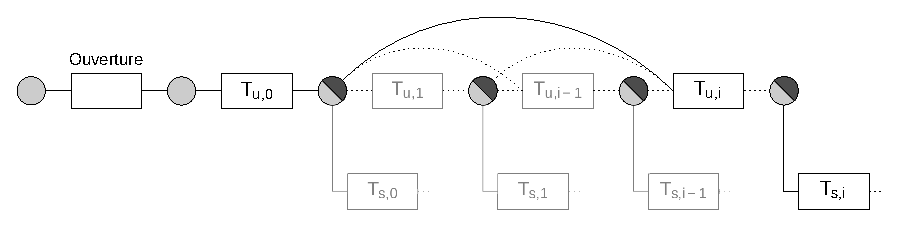
\includegraphics[scale=0.7]{img/eltoo-offchain-protocol.eps}
  \caption{Aperçu du protocole Eltoo.}
\end{figure}

Une transaction supplémentaire est ajoutée à la chaîne de transactions pour éviter que le délai d'expiration des transactions de règlement $T_{s,i}$ soit atteint et qu'elles soient diffusées sur la chaîne. Cette transaction envoie simplement les fonds vers un compte multisignatures classique, et est signée et diffusée après la signature des premières transactions de mise à jour et de règlement ($T_{u,0}$ et $T_{s,0}$). Le délai d'expiration ne commence que lorsque la transaction $T_{u,0}$ est diffusée.

Ce fonctionnement permet d'obtenir un protocole simple de mise à jour du canal, peu contraignant pour les nœuds, sans mécanisme de punition, et permettant de ne pas à avoir à décider les frais à l'avance. Cette facilité d'implémentation pourrait rendre plus aisée la création de contrats plus complexes sur Lightning, comme les canaux de paiement à 3 participants ou plus. En outre, leur implémentation de doit en aucun remplacer celle des canaux de Poon-Dryja~: les deux modèles peuvent coexister au sein d'un seul et même réseau de canaux de paiement.

Les transactions flottantes sont implémentées à l'aide de \texttt{SIGHASH\_ALL | SIGHASH\_ANYPREVOUT}. \textcolor{darkgray}{La mise en œuvre de Eltoo repose donc sur l'intégration du BIP-118 à Bitcoin.}

\section*{L'inscription de données arbitraires}
\addcontentsline{toc}{section}{L'inscription de données arbitraires}

% Données arbitraire
Bitcoin permet d'inscrire des données non financières sur la chaîne, c'est-à-dire des données qui ne sont pas nécessaires dans le blocage et dans la rédemption des fonds et qui sont interprétées de manière extérieure. Même en imposant toutes les restrictions possibles, on ne pourrait pas empêcher l'inscription de ces données, même si on pourrait la rendre plus coûteuse.

% Laisser sa marque pour la postérité
La chaîne de blocs est largement partagée autour du monde, et sera conservée par l'humanité, au moins comme un reliquat historique, de sorte qu'on peut supposer que ce qui y est stocké sera conservé très longtemps. Cette caractéristique pousse les gens à chercher à y inclure des choses qui leur tiennent à cœur. Il est dans la nature de l'homme de chercher à laisser des traces de son passage sur Terre et écrire sur la chaîne principale de Bitcoin est une manière de le faire.

% Méthodes d'inscription
Il existe diverses méthodes d'inscription, qui ont chacune leurs qualités et leurs défauts. Celles-ci ont évolué au fur et à mesure des années, alors que cette utilisation se libéralisait\sendnote{Andrew Sward, Ivy Vecna, Forrest Stonedahl, \eng{Data Insertion in Bitcoin's Blockchain}, 3 avril 2018~: \url{https://doi.org/10.5195/ledger.2018.101}.}.

% Inscription dans la base de pièce par les mineurs
D'une part, l'écriture de données arbitraires peut être réalisée par les mineurs au sein de la base de pièce, l'entrée de transaction de récompense. C'est cette méthode dont Satoshi Nakamoto a fait usage pour inscrire le désormais célèbre titre de une du Times du 3 janvier 2009 dans le bloc de genèse~:

\begin{Verbatim}[fontsize=\footnotesize]
The Times 03/Jan/2009 Chancellor on brink of second bailout for banks
\end{Verbatim}

% Inscriptions par les mineurs
D'autres blocs contiennent des messages emblématiques. Le bloc d'exode de BCH contenait un message de bienvenue pour Shuya Yang, la fille du PDG de la coopérative ViaBTC\sendnote{Bitcoin Cash, bloc 478~559~: «~\eng{Welcome to the world, Shuya Yang!}~».}. Le bloc 629~999, le bloc précédant le troisième halving sur BTC en 2020, contenait le titre d'un article du New York Times du 9 avril annonçant l'injection de liquidité record de la Réserve Fédérale (2~300 milliars de dollars) en réaction à la crise du Covid-19\sendnote{Bitcoin-BTC, bloc 629~999~: «~\eng{NYTimes 09/Apr/2020 With \$2.3T Injection, Fed's Plan Far Exceeds 2008 Rescue}~»}.

Le champ de la base de pièce peut être utilisé pour écrire d'autres données. C'est le cas du nonce supplémentaire (le critère qui a permis d'identifier les bitcoins de Satoshi\sendnote{Sergio Lerner, \eng{The Well Deserved Fortune of Satoshi Nakamoto, Bitcoin creator, Visionary and Genius}, 17 avril 2013~: \url{https://bitslog.com/2013/04/17/the-well-deserved-fortune-of-satoshi-nakamoto/}.}). C'est aussi le cas du signalement des coopératives minières qui est réalisé dans ce champ~: par exemple, la base de pièce du bloc 751~005 contient la chaîne de caractères \texttt{poolin.com}, ce qui indique que sa validation a probablement été réalisée par la coopérative chinoise Poolin.

% Inscription par les utilisateurs
D'autre part, le privilège d'écrire des données arbitraires sur la chaîne n'est pas réservé aux mineurs. Les simples utilisateurs peuvent aussi le faire à condition de payer les frais correspondants.

% Stockage dans les sorties transactionnelles (P2PKH, P2MS et P2SH)
Avant 2014, on procédait la plupart du temps à ces inscriptions en stockant les données dans les scripts de verrouillage, par exemple par l'utilisation de l'instruction de dépilement \texttt{OP\_DROP}\sendnote{La transaction \longstring{c0b2cf75b47d1e7f48cdb4287109ff1dd5bcf146d5f77a9e8784c0c9c0ef02ad}, confirmée le 13 décembre 2012, contient par exemple la chaîne de caractères \texttt{TheCakeIsALie\textbackslash{}n} en référence au jeu vidéo Portal.}. Une autre pratique courante était d'inscrire les données dans les sorties de type P2PKH qui étaient rendues indépensables au passage. Cette méthode était extrêmement coûteuse en raison de la forme de la transaction (imposant l'inscription dans les sorties transactionnelles) et le fait de devoir envoyer des montants non nuls en sortie. Elle était également dommageable pour le système dans son ensemble, car elle encombrait l'ensemble des UTXO.

% Instruction OP_RETURN (première utilisation en mars 2013 : 1a2e22a717d626fc5db363582007c46924ae6b28319f07cb1b907776bd8293fc)
En mars 2014, l'arrivée de la version 0.9.0 de Bitcoin Core a rendu standarde l'instruction \texttt{OP\_RETURN}, dont l'effet est de mettre fin à l'exécution du script\sendnote{L'instruction \texttt{OP\_RETURN} servait initialement à retourner la valeur au sommet de la pile, d'où son nom. Cependant, en juillet 2010, la découverte du «~\eng{1 RETURN bug}~», qui permettait de dépenser toute sortie transactionnelle via le script de déverrouillage \texttt{TRUE RETURN}, a poussé Satoshi Nakamoto à désactiver cette fonctionnalité en lui faisant renvoyer \texttt{FALSE} systématiquement (\url{https://github.com/bitcoin/bitcoin/commit/a75560d828464c3f1138f52cf247e956fc8f937d}).}. Ce changement permettait de créer «~une sortie assurément élagable, pour éviter les schémas de stockage de données [...] qui stockaient des données arbitraires telles que des images en tant que sorties transactionnelles éternellement indépensables, gonflant ainsi la base de données des UTXO de bitcoin\sendnote{\eng{Bitcoin Core version 0.9.0 released}, 19 mars 2014~: \url{https://bitcoin.org/en/release/v0.9.0\#opreturn-and-data-in-the-block-chain}.}~». % "The OP_RETURN change creates a provably-prunable output, to avoid data storage schemes – some of which were already deployed – that were storing arbitrary data such as images as forever-unspendable TX outputs, bloating bitcoin's UTXO database."

\textbf{NULLDATA} Le schéma résultant, appelé NULLDATA (signifiant littéralement «~données insignifiantes~»), est désormais un moyen standard d'inscrire des informations sur la chaîne dans une limite de 80~octets par transaction\sendnote{Dans BTC, la taille des données suivant \texttt{OP\_RETURN} est de \textcolor{darkgray}{83 octets} (règle de mempool), donnant la possibilité d'inscription de 80 octets de données arbitraires.}. Il est identifié par la présence de l'opérateur \texttt{OP\_RETURN} suivi de données empilées~:

\begin{Verbatim}[fontsize=\small]
RETURN [données arbitraires]
\end{Verbatim}

Ce type de sortie est exempt de la limite standarde de poussière, qui est \textcolor{darkgray}{actuellement de 546 satoshis pour les sorties P2PKH}, de façon à pouvoir créer une sortie de 0 satoshis et ne pas gaspiller des fonds inutilement.

% Stockage dans les entrées transactionnelles : P2SH, P2WPKH, P2WSH, P2TR
En outre, il est aussi possible de stocker des données au sein des entrées transactionnelles ou des les témoins liés, lors de la dépense de sorties P2SH, P2WSH ou P2TR. Cette écriture peut se faire dans les scripts de récupération ou bien dans les éléments de déverrouillage. Cette méthode a l'avantage de ne pas surcharger l'ensemble des UTXO. Côté utilisateur, dans où SegWit s'applique, elle a pour bénéfice de diviser le coût des données arbitraires inscrites dans la transactions par quatre.

% --- Inscriptions ---

Ces différentes méthodes ont été utilisées pour inscrire toutes sortes de choses sur la chaîne, dont notamment des empreintes cryptographiques, du texte et des images\sendnote{Ken Shirriff, \eng{Hidden surprises in the Bitcoin blockchain and how they are stored: Nelson Mandela, Wikileaks, photos, and Python software}, 16 février 2014~: \url{https://www.righto.com/2014/02/ascii-bernanke-wikileaks-photographs.html}.}.

% Horodatage par inscription d'empreintes
D'abord, on peut inscrire une empreinte, l'inscription servant alors à l'horodatage. Il s'agit d'inscrire l'empreinte d'un fichier sur la chaîne en tant que preuve d'existence. Cette idée a été mise en avant en février 2009 par Hal Finney dans un de ses courriels adressés à la liste de diffusion dédiée à Bitcoin. Il suggérait alors que «~la pile de blocs de bitcoin serait parfaite~» pour «~prouver qu'un certain document a existé à un certain moment dans le passé\sendnote{Hal Finney, \eng{Re: [bitcoin-list] Bitcoin v0.1.5 released}, \wtime{27/02/2009 20:00:12 UTC}, archive~: \url{https://web.archive.org/web/20131016004925/http://sourceforge.net/p/bitcoin/mailman/bitcoin-list/?viewmonth=200902}.}~», un point de vue approuvé par Satoshi\sendnote{«~En effet, Bitcoin est un serveur d'horodatage sécurisé et distribué pour les transactions. Quelques lignes de code pourraient créer une transaction avec une empreinte supplémentaire de tout ce qui doit être horodaté. Je devrais ajouter une commande pour horodater un fichier de cette façon.~» -- Satoshi Nakamoto, \eng{Re: [bitcoin-list] Bitcoin v0.1.5 released}, \wtime{04/03/2009 16:59:12 UTC}, archive~: \url{https://web.archive.org/web/20131016004648/http://sourceforge.net/p/bitcoin/mailman/bitcoin-list/?viewmonth=200903}.}. % "BTW I don't remember if we talked about this, but the other day some people were mentioning secure timestamping. You want to be able to prove that a certain document existed at a certain time in the past. Seems to me that bitcoin's stack of blocks would be perfect for this." -- "Indeed, Bitcoin is a distributed secure timestamp server for transactions.  A few lines of code could create a transaction with an extra hash in it of anything that needs to be timestamped. I should add a command to timestamp a file that way."

En somme, cette pratique permet de démontrer la connaissance d'une information avant sa publication, et donc indirectement qu'on en est l'auteur probable. Ce type d'usage est notamment mis en œuvre par l'entreprise française Woleet.

% Empreintes pour IPFS
Cet usage peut aussi être exploité par les systèmes décentralisés d'hébergement de fichiers, comme le système IPFS (InterPlanetary File System) qui utiliser les empreintes des fichiers pour les identifier et permettre leur stockage par un réseau pair-à-pair d'utilisateurs. Il est donc possible d'associer le texte écrit sur la chaîne de blocs et des images ou des vidéos, hébergées de manière décentralisée.

% Texte
Ensuite, on peut inscrire un texte, qui est généralement encodé en ASCII~/~UTF-8. Par exemple, la phrase «~Il est possible d'écrire des données arbitraires sur toutes les chaînes.~» a été inscrite sur la chaîne de BTC le 3 décembre 2019\sendnote{Transaction d'identifiant \longstring{9f4482bf9a8ac9233eef676e7746787cc420620f855f97643ea812a53ca561a3}.}. L'inscription de textes permet aussi de dessiner des images en art ASCII. C'est le cas de l'hommage à Len Sassaman, décédé en juillet 2011, qui a été inscrit sur la chaîne par les développeurs Dan Kaminsky et Travis Goodspeed par le biais de sorties P2PKH\sendnote{Cet hommage peut être retrouvé dans la transaction d'identifiant \longstring{930a2114cdaa86e1fac46d15c74e81c09eee1d4150ff9d48e76cb0697d8e1d72} confirmée le 30 juillet 2011.}, et qui contient notamment une représentation du président de la Fed d'alors, Ben Bernanke~:

\begin{Verbatim}[fontsize=\small]
---BEGIN TRIBUTE---  =-=-=-=-=-=-=-=-=-=     ASCII BERNANKE
#./BitLen            LEN "rabbi" SASSAMA  :'::.:::::.:::.::.:
:::::::::::::::::::       1980-2011       : :.: ' ' ' ' : :':
:::::::.::.::.:.:::  Len was our friend.  :.:     _.__    '.:
:.: :.' ' ' ' ' : :  A brilliant mind,    :   _,^"   "^x,   :
:.:'' ,,xiW,"4x, ''  a kind soul, and     '  x7'        `4,
:  ,dWWWXXXXi,4WX,   a devious schemer;    XX7            4XX
' dWWWXXX7"     `X,  husband to Meredith   XX              XX
 lWWWXX7   __   _ X  brother to Calvin,    Xl ,xxx,   ,xxx,XX
:WWWXX7 ,xXX7' "^^X  son to Jim and       ( ' _,+o, | ,o+,"
lWWWX7, _.+,, _.+.,  Dana Hartshorn,       4   "-^' X "^-'" 7
:WWW7,. `^"-" ,^-'   coauthor and          l,     ( ))     ,X
 WW",X:        X,    cofounder and         :Xx,_ ,xXXXxx,_,XX
 "7^^Xl.    _(_x7'   Shmoo and so much      4XXiX'-___-`XXXX'
 l ( :X:       __ _  more.  We dedicate      4XXi,_   _iXX7'
 `. " XX  ,xxWWWWX7  this silly hack to     , `4XXXXXXXXX^ _,
  )X- "" 4X" .___.   Len, who would have    Xx,  ""^^^XX7,xX
,W X     :Xi  _,,_   found it absolutely  W,"4WWx,_ _,XxWWX7'
WW X      4XiyXWWXd  hilarious.           Xwi, "4WW7""4WW7',W
"" ,,      4XWWWWXX  --Dan Kaminsky,      TXXWw, ^7 Xk 47 ,WH
, R7X,       "^447^  Travis Goodspeed     :TXXXWw,_ "), ,wWT:
R, "4RXk,      _, ,  P.S.  My apologies,  ::TTXXWWW lXl WWT:
TWk  "4RXXi,   X',x  BitCoin people.  He  ----END TRIBUTE----
lTWk,  "4RRR7' 4 XH  also would have
:lWWWk,  ^"     `4   LOL'd at BitCoin's
::TTXWWi,_  Xll :..  new dependency upon
\end{Verbatim}

% Images
Enfin, on peut inscrire une image, qui peut être encodée dans de multiples formats, dont notamment en JPEG ou en PNG. Un logo Bitcoin datant du 13 mai 2011 peut être retrouvé\sendnote{Transactions \longstring{ceb1a7fb57ef8b75ac59b56dd859d5cb3ab5c31168aa55eb3819cd5ddbd3d806} et \longstring{9173744691ac25f3cd94f35d4fc0e0a2b9d1ab17b4fe562acc07660552f95518}}. Un hommage à Nelson Mandela accompagné d'une photo a été publié le 7 décembre 2013, quelques jours après sa mort\sendnote{Transactions \longstring{8881a937a437ff6ce83be3a89d77ea88ee12315f37f7ef0dd3742c30eef92dba}.}. En 2022, l'absence de restriction standarde sur la taille des scripts de Taproot a permis de réaliser des inscriptions volumineuses d'une manière bien plus transparente et directe. C'est ce qui a notamment permis d'inscrire l'image des Taproot Wizards qui pesait quasiment 4~Mo (voir figure~\ref{fig:taproot-wizards}).

\begin{figure}[h]
  \centering
  
\includegraphics[scale=0.6]{img/taproot-wizards-small-0301e0480b374b32851a9462db29dc19fe830a7f7d7a88b81612b9d42099c0aei0.jpg}
  \caption{Image (réduite) des Taproot Wizards.}
  \label{fig:taproot-wizards}
\end{figure}

% Autres fichiers
De manière générale, tout format de fichier peut être stocké sur la chaîne au travers de transactions multiples~: un document\sendnote{Le PDF du livre blanc de Bitcoin a été inscrit sous forme de sorties P2MS au sein de la transaction \longstring{54e48e5f5c656b26c3bca14a8c95aa583d07ebe84dde3b7dd4a78f4e4186e713}, le 6 avril 2013.}, un livre, une vidéo, un jeu\sendnote{Nicholas Carlini, \eng{Yet Another Doom Clone}, 1\ier{} février 2023~: \url{https://ordinals.com/inscription/521f8eccffa4c41a3a7728dd012ea5a4a02feed81f41159231251ecf1e5c79dai0}, \url{https://nicholas.carlini.com/writing/2019/javascript-doom-clone-game.html}.}, etc.

% Pertinence de cet usage
Cependant, cet usage n'est pas forcément toujours pertinent. L'inscription demande le paiement de frais, parfois élevés, et n'est pas franchement fait pour conserver des données volumineuses. La publication sur IPFS et sur serveur local est généralement bien plus opportune.

% Bitcoin SV
La communauté de Bitcoin SV s'est spécialisée dans cette utilisation, considérant que son registre était une «~source universelle de vérité\sendnote{CoinGeek, \eng{Jerry Chan: Bitcoin’s value is as a universal source of truth}, 17 juillet 2019~: \url{https://coingeek.com/jerry-chan-bitcoins-value-is-as-a-universal-source-of-truth-video/}.}~». Ainsi, on peut retrouver un volume assez importants de données météorologiques sur sa chaîne, qui y sont inscrites depuis 2019\sendnote{Helen Partz, \eng{98\% of BSV Transactions Used for Writing Weather Data on Blockchain: Report}, 24 juin 2019~: \url{https://cointelegraph.com/news/98-of-bsv-transactions-used-for-writing-weather-data-on-blockchain-report}.}.

\section*{Les métaprotocoles}
\addcontentsline{toc}{section}{Les métaprotocoles}

% Définition
Les métaprotocoles sont des protocoles qui se servent du protocole de base pour fonctionner. Ils font usage de l'inscription de données arbitraires sur la chaîne pour inclure des instructions qui sont interprétées par des implémentations logicielles spécifiques\sendnote{C'est en ce sens que les métaprotocoles peuvent être appelés des surcouches, même si on préfère généralement utiliser ce terme pour parler des systèmes comme Lightning par exemple.}. Ils ont pour particularité d'être nécessairement plus extensifs que le protocole de base.

% Bitcoin 2.0
Ce n'est pas une idée nouvelle. Dès les premières années d'existence de Bitcoin, certaines personnes ont été désireuses de l'exploiter plus en profondeur, de se servir de lui d'une autre manière que comme un instrument de transfert de valeur. Ce mouvement initial était appelé «~Bitcoin 2.0~» par certains, et il a par la suite mené à l'élaboration d'Ethereum à partir de 2013.

% Colored Coins
Le premier type de métaprotocole qui a été élaboré est le procédé des \eng{colored coins}, ou pièces colorées en français, qui consiste à marquer des pièces (UTXO) par des données inscrites. Chaque type de jeton créé est liée à un identifiant, que l'on peut assimiler à une couleur, d'où le nom de ce procédé. L'idée est apparue en 2012\sendnote{Yoni Assia, \eng{bitcoin 2.X (aka Colored Bitcoin) – initial specs}, 27 mars 2012~: \url{https://yoniassia.com/coloredbitcoin/}~; Meni Rosenfeld, \eng{Overview of Colored Coins}, 4 décembre 2012~: \url{https://bitcoil.co.il/BitcoinX.pdf}.}. % inscrites notamment par l'utilisation de l'opérateur \texttt{OP\_RETURN}

\textcolor{brown}{schéma colored coin}

% Implémentation des colored coins
L'implémentation de cette idée a été réalisée dès la fin de l'année 2012 par l'intermédiaire du ChromaWallet\sendnote{Alex Mizrahi, \eng{ChromaWallet (colored coins): issue and trade private currencies/stocks/bonds/..}, \wtime{07/09/2012 12:46:12 UTC}~: \url{https://bitcointalk.org/index.php?topic=106373.msg1167516\#msg1167516}.}. Mais elle n'a vraiment pris de l'ampleur qu'à partir de 2014, avec l'apparition des Open Assets de Coinprism, des \eng{CoinSpark assets} de Coin Sciences, et des Colored Coins de Colu. Ces usages sont depuis tombés en désuétude, même si le procédé a pu servir de manière sporadique au fil des années, comme dans le cas du jeton BSQ de Bisq créé en 2018 comme base de sa DAO. Une tentative de restauration a également été faite sur Bitcoin Cash avec les jetons SLP, sans grand succès. % Open Assets (\texttt{OA}), Colored Coins (\texttt{CC}), CoinSpark assets (\texttt{SPK})

% Mastercoin et Counterparty
Au-delà des pièces colorées, il existait également des protocoles plus évolués qui avaient la particularité de gérer une unité de compte propre. Il s'agissait essentiellement de Mastercoin, qui a été renommé en Omni en mars 2015, et de Counterparty.

% Mastercoin, 2013
Le premier métaprotocole de ce type a été Mastercoin\sendnote{Le mot «~master~» dans le nom de Mastercoin est l'acronyme de «~\eng{Metadata Archival by Standard Transaction Embedding Records}~», d'après les spécifications techniques~: \url{https://github.com/OmniLayer/spec/blob/master/OmniSpecification-v0.6.adoc}.}, dont le livre blanc, intitulé «~\eng{The Second Bitcoin Whitepaper}~», a été publié le 6 janvier 2012 par J.R. Willett\sendnote{J.R. Willett, \eng{[It's here] The Second Bitcoin Whitepaper}, \wtime{06/01/2012 22:42:24 UTC}~: \url{https://bitcointalk.org/index.php?topic=56901.msg678427\#msg678427}~; J.R. Willett, \eng{The Second Bitcoin Whitepaper}, 6 janvier 2012~: \url{https://cryptochainuni.com/wp-content/uploads/Mastercoin-2nd-Bitcoin-Whitepaper.pdf}.}. Il s'agissait d'un protocole permettant à ses utilisateurs de créer leurs propres devises, appelées «~\eng{user currencies}~».

% MSC et ICO
Mastercoin reposait sur une unité de compte notée le MSC, qui a fait l'objet d'une prévente d'un mois en juillet-août 2013\sendnote{Tous les bitcoins envoyés à l'adresse \longstring{1EXoDusjGwvnjZUyKkxZ4UHEf77z6A5S4P} étaient transformés en MSC à raison de 100~MSC au début, taux dégressif au fil des semaines. }. C'était la première \eng{Initial Coin Offering} de l'histoire, et elle a recueilli 5120~BTC, soit plus de 500~000~\$ à ce moment-là.

% USDT
Le plus grand succès de ce protocole a probablement été la création du premier stablecoin, le Tether USD, qui a été émis sous le nom de Realcoin en octobre 2014. Mastercoin~/~Omni a longtemps été l'unique manière de posséder et de transférer de l'USDT avant que le jeton ne soit émis massivement sur d'autres chaînes comme Ethereum et Tron.

% Counterparty, 2014
Le second métaprotocole avancé a été Counterparty, lancé en janvier 2014. Cette plateforme reposait également sur un jeton natif, le XCP, qui lui servait de carburant, et qui a été créé par brûlage de bitcoins durant son premier mois d'existence\sendnote{Tous les bitcoins envoyés à l'adresse \longstring{1CounterpartyXXXXXXXXXXXXXXXUWLpVr} entre le 2 janvier et le 3 février 2014 étaient convertis en XCP à un taux qui variait entre 1000 et 1500~XCP par BTC}. Ce sont 2140~bitcoins qui ont ainsi été rendus inutilisables pour donner vie à plus de 2,6~millions de XCP, encore en circulation aujourd'hui. Counterparty se voulait plus flexible que Mastercoin en rendant possible l'implémentation de contrats autonomes, notamment dans le but de créer des jetons et d'héberger des plateformes d'échange décentralisées, appelées des «~distributeurs~».

% Jetons non fongibles (NFT)
En particulier, Counterparty a été la première plateforme à proposer la gestion de jetons non fongibles (NFT). Il s'agissait là de mettre en œuvre une vieille idée, qui avait notamment été mise en valeur par Hal Finney en 1993 sur la liste de diffusion cypherpunk sous la forme de «~cartes à collectionner cryptographiques\sendnote{Hal Finney, \eng{Crypto trading cards.}, \wtime{17/01/1993 18:48:02 UTC}~: \url{https://cypherpunks.venona.com/date/1993/01/msg00152.html}.}~». Counterparty a ainsi hébergé une multitude de collections de tels objets, comme les cartes à jouer de \eng{Spells of Genesis} et de SaruTobi créées en 2015, ou les Rare Papes émis entre 2016 et 2018\sendnote{Vlad Costea, \eng{Bitcoin NFTs On Counterparty (And How To Get Or Create Your First One)}, 29 décembre 2021~: \url{https://bitcoin-takeover.com/bitcoin-nfts-on-counterparty-and-how-to-get-or-create-your-first-one/}.}.

% Memo, 2018
En 2018, l'apparition de Bitcoin Cash a motivé la création d'un média social dont les données seraient entièrement stockées sur la chaîne, les développeurs de BCH étant plus libéraux à ce sujet. Le protocole s'appelait Memo et consistait à publier de courts messages visibles publiquement sous un profil défini et à pouvoir suivre les autres utilisateurs, à aimer et répondre à leurs messages. L'idée était d'obtenir une sorte de réseau social résistant à la censure, mais souffrait néanmoins de la nécessité de payer des frais. \sendnote{Le protocole Memo est disponible à l'adresse~: \url{https://memo.cash/protocol}.}

% Ordinals, 2023
Tous ces protocoles ont perdu de leur jusqu'à l'apparition du protocole Ordinals, lancé en janvier 2023. Ce métaprotocole permettait de créer et de gérer des «~artefacts numériques~», c'est-à-dire de NFT dont l'intégralité des données est stockée de manière immuable sur une chaîne résistante à la censure. Le protocole Ordinals reposait sur une «~théorie des ordinaux~» permettant de suivre et de transférer des satoshis liés à une inscription, comme un texte, un image ou autre chose\sendnote{\url{https://docs.ordinals.com/}}. En particulier, Ordinals a été utilisé pour émuler la propriété et le transfert de jetons fongibles, baptisés «~BRC-20~», dont le succès spéculatif a provoqué une congestion du réseau menant à une hausse des frais de transaction record.

% STAMPS, 2023
Le succès d'Ordinals a également inspiré la création du protocole STAMPS, qui se basait sur Counterparty pour le suivi des artefacts et stockait leurs données dans des sorties P2MS\sendnote{STAMP est l'acronyme de \eng{Secure, Tradeable Art Maintained Permanently}. -- Mike In Space, \eng{STAMPS: A Protocol for Storing Images On-Chain in Transaction Outputs Immutably on Bitcoin}, 6 avril 2023~: \url{https://github.com/mikeinspace/stamps/tree/main}.}.

% Opposition
Toutes ces pratiques ont créé des débats. En effet, Bitcoin était présenté comme un modèle de monnaie numérique et il semblait contreproductif d'en faire un protocole de conservation de données qui ne seraient pas relatives au transfert de bitcoins. Ainsi, dès décembre 2010, Jeff Garzik s'opposait au fait d'utiliser la chaîne pour le stockage généralisé\sendnote{Jeff Garzik, \eng{Resist the urge to use block chain for generalized storage}, \wtime{07/12/2010 22:04:54 UTC}~: \url{https://bitcointalk.org/index.php?topic=2129.msg27884\#msg27884}.}. Plus tard, en 2014, des disputes similaires ont éclaté au sujet de Counterparty\sendnote{BitMEX Research, \eng{The OP\_Return Wars of 2014 – Dapps Vs Bitcoin Transactions}, 12 juillet 2022~: \url{https://blog.bitmex.com/dapps-or-only-bitcoin-transactions-the-2014-debate/}.}. En 2023, c'est également la même discorde qui a eu lieu à la suite du succès d'Ordinals\sendnote{pourteaux, \eng{Illegitimate bitcoin transactions}, 25 janvier 2023~: \url{https://read.pourteaux.xyz/p/illegitimate-bitcoin-transactions}.}.

% Premier défaut : manque de vérification
Ces métaprotocoles ont deux défauts majeurs. Le premier est que la vérification de leurs règles dépend d'un petit sous-ensemble de nœuds du réseau. En effet, la gestion d'un tel protocole construit en surcouche demande des ressources supplémentaires, notamment en ce qui concerne l'indexation pour les pièces colorées. De ce fait, peu de personnes déploient une implémentation complète, ce qui centralise considérablement le protocole et le rendent sensible à la modification par un adversaire, notamment pour y inclure de la censure.

% Second défaut : frais
Le second défaut est leurs frais d'utilisation parfois très élevés, surtout si la limite de capacité transactionnelle du réseau est atteinte. Les transactions mettant en place ces solutions sont nécessairement plus volumineuses que les transactions normales et entraînent par conséquent des frais plus élevés. Elles sont donc plus facilement exclues par l'augmentation des frais issue de la congestion du réseau.

% Conséquences de ces défauts
C'est pour ces raisons que les personnes qui ont travaillé sur ces solution s'en sont vite détournées, préférant se réfugier vers des plateformes alternatives comme NXT et surtout Ethereum. Vitalik Buterin lui-même s'intéressait aux pièces colorées et à Mastercoin en 2013 avant de commencer à bâtir ce qui allait devenir Ethereum\sendnote{Yoni Assia, Vitalik Buterin, Meni Rosenfeld, Rotem Lev, \eng{Colored Coins whitepaper}, 2013~: \url{http://www.ma.senac.br/wp-content/uploads/2018/05/ColoredCoinswhitepaper-DigitalAssets.pdf}~; Vitalik Buterin, \eng{A Prehistory of the Ethereum Protocol}, 14 septembre 2017~: \url{https://vitalik.ca/general/2017/09/14/prehistory.html}.}. C'est aussi pour ces raisons que des solutions moins coûteuses (des surcouches utilisant la chaîne comme un procédé de règlement et non pas comme un lieu où inscrire toutes les opérations) sont aujourd'hui privilégiées pour faire ce genre de choses comme RGB ou Taro.

\section*{Les contrats hors chaîne} % Scriptless Scripts, Taproot et RGB
\addcontentsline{toc}{section}{Les contrats hors chaîne}

% Mise à niveau Schnorr-Taproot
La cryptographie permet de déployer des contrats sans que ceux-ci ne doivent être inscrits sur la chaîne. Cette particularité a été facilitée grâce à la mise à niveau Schnorr-Taproot, souvent appelée simplement Taproot, qui est survenue sur BTC le 14 novembre 2021 et qui incluait deux éléments majeurs~: le schéma de signature de Schnorr et le procédé de programmation de contrats Taproot. Ces fonctionnalités ont été intégrées sous forme d'un soft fork au sein du schéma standard P2TR correspondant à la version 1 de SegWit.

% Schéma de signature de Schnorr
Le schéma de Schnorr implémenté est une dérivation du protocole d'authentification du même nom décrit en 1989 par Claus-Peter Schnorr. Il s'agit d'une alternative à ECDSA qui se base sur la même courbe elliptique (\texttt{secp256k1}) et qui permet de signer des transactions grâce aux mêmes paires de clés.

% Avantages des signatures de Schnorr
Comparé à ECDSA, le schéma de signature de Schnorr possède quelques avantages. Premièrement, il produit des signatures moins grandes. Deuxièmement, les signatures produites sont non-malléables, le procédé ne faisant pas intervenir de nombre aléatoire. Troisièmement, et c'est le plus important, il présente une propriété de linéarité, ce qui permet notamment de faire des choses comme la vérification par lots et l'agrégation des clés. \sendnote{Pieter Wuille, Jonas Nick, Tim Ruffing, \eng{Schnorr Signatures for secp256k1}, 19 janvier 2020~: \url{https://github.com/bitcoin/bips/blob/master/bip-0340.mediawiki}.}

% Pourquoi Schnorr n'a pas été intégré dans Bitcoin
Le schéma de Schnorr est supérieur à ECDSA et existait en 2008, mais Satoshi Nakamoto n'a pas daigné s'en servir. Ce choix s'explique par le fait que l'algorithme était breveté aux États-Unis jusqu'en février 2008 et que par conséquent il n'existait pas d'implémentation standardisée. Le logiciel de Bitcoin utilisait en effet OpenSSL, qui n'intégrait pas ce type d'algorithme.

% Scriptless Scripts
Le schéma de Schnorr autorise le déploiement de \eng{Scriptless Scripts}, de contrats «~sans script~» qui sont exécutés en dehors de la chaîne et appliqués au sein des signatures. Le concept a été théorisé en 2017 par Andrew Poelstra\sendnote{Andrew Poelstra, \eng{Using the Chain for what Chains are Good For}, Scaling Bitcoin IV, 5 novembre 2017~: \url{https://www.youtube.com/watch?v=3pd6xHjLbhs\&t=5755s}~; Aaron van Wirdum, \eng{Scriptless Scripts: How Bitcoin Can Support Smart Contracts Without Smart Contracts}, 27 novembre 2017~: \url{https://bitcoinmagazine.com/technical/scriptless-scripts-how-bitcoin-can-support-smart-contracts-without-smart-contracts}.}. Il se retrouve dans des exemples comme le schéma de multisignature MuSig2\sendnote{Jonas Nick, Tim Ruffing, Yannick Seurin, \eng{MuSig2: Simple Two-Round Schnorr Multi-Signatures}, 14 octobre 2020~: \url{https://eprint.iacr.org/2020/1261.pdf}.}, les \eng{adaptor signatures} ou encore les \eng{Discreet Log Contracts}\sendnote{Thaddeus Dryja, \eng{Discreet Log Contracts}, 2017~: \url{https://adiabat.github.io/dlc.pdf}.}.

% Taproot
Outre cela, le schéma de Schnorr facilite grandement l'implémentation de Taproot, qui a été intégré au protocole au même moment. Taproot (dont le nom signifie littéralement «~racine pivot~» en français) est un système d'arbres syntaxiques abstraits merkélisés permettant d'ancrer les clauses d'un contrat au sein d'un arbre de Merkle et de cacher cet arbre sous une clé publique agrégée appartenant à ses participants. Il permet ainsi de ne publier le contrat qu'en cas de litige, et même dans ce cas, de ne publier que les conditions exécutées\sendnote{Pieter Wuille, Jonas Nick, Anthony Towns, \eng{Taproot: SegWit version 1 spending rules}, 19 janvier 2020~: \url{https://github.com/bitcoin/bips/blob/master/bip-0341.mediawiki}.}. Les scripts utilisés dans Taproot utilisent un langage de programmation nommé Tapscript, basé sur le langage de script classique de Bitcoin\sendnote{Pieter Wuille, Jonas Nick, Anthony Towns, \eng{Validation of Taproot Scripts}, 19 janvier 2020~: \url{https://github.com/bitcoin/bips/blob/master/bip-0342.mediawiki}.}.

% MAST
Un arbre syntaxique abstrait merkélisé (aussi appelés MAST pour \eng{Merklized Abstract Syntax Tree}) est un arbre de hachage (voir chapitre~\ref{ch:confirmation}) qui contient les empreintes des clauses (conditions de dépense). Lors de l'exécution du MAST, l'utilisateur a seulement besoin de révéler la clause appliquée, ce qui lui permet de dépenser les fonds, et de fournir les empreintes liées aux autres conditions sans les dévoiler.

\textcolor{brown}{schéma MAST : 5 clauses, fermeture coopérative multisig 5-parmi-5 (bonne pratique) et autres conditions}

% Historique
L'implémentation des MAST au sein de Bitcoin avait déjà été proposée par le passé, que ce soit sous la forme d'une nouvelle version de SegWit (BIP-114), ou bien d'un nouvel code opération \texttt{OP\_MERKLEBRANCHVERIFY} (BIP-116, BIP-117). Mais Taproot a constitué une proposition supérieure en permettant de ne pas révéler l'existence du MAST lui-même.

% Racine pivot
Taproot autorise la dépense coopérative par la modification légère (\eng{tweaking}) de la clé publique agrégée interne à l'aide de la racine du MAST. La clé obtenue est celle inscrite dans le script de verrouillage de la pièce, de sorte qu'elle est indiscernable des autres sorties P2TR. De même, la signature agrégée est indiscernable d'une signature classique. Taproot constitue ainsi une façon de régler les contrats en dehors de la chaîne, tant qu'il n'y a pas de litige.

% RGB
Au-delà de Taproot, une alternative est RGB, qui est un système de contrats autonomes hors chaîne, construit à la fois en surcouche de Bitcoin et de Lightning. Le nom est issu du standard RGB (\eng{Red Green Blue}) qui permet de définir une couleur et constitue par conséquent une référence directe aux \eng{colored coins}, RGB ayant été originellement conçu comme «~une meilleure version des pièces colorées\sendnote{RGB FAQ, \eng{What does 'RGB' stand for?}, 14 décembre 2020~: \url{https://www.rgbfaq.com/faq/what-does-rgb-stand-for}.}~». Cependant, même si RBG permet effectivement d'émettre et de gérer des jetons, cette fonctionnalité est loin d'être la seule.

RGB se base sur deux primitives techniques conceptualisées en 2016 par le développeur Peter Todd\sendnote{\url{https://petertodd.org/2016/state-machine-consensus-building-blocks#uniqueness-and-single-use-seals}~; \url{https://petertodd.org/2016/closed-seal-sets-and-truth-lists-for-privacy}.}~: la validation côté client (\eng{client-side validation}) et les scellés à usage unique (\eng{single-use seals}). Cela permet la gestion d'un état indépendant, pour lequel la double dépense est empêchée par ces scellés. Après fait l'objet de recherches par Giacomo Zucco et le BHB Network, RGB est actuellement développé par la LNP/BP Standards Association.

% Avantages généraux
L'implémentation de contrats en dehors de la chaîne est donc possible sur Bitcoin. Et ils apportent deux choses. D'une part, ils réduisent le paiement de frais en ayant une empreinte minimale sur la chaîne. D'autre part, ils améliorent la confidentialité de leurs participants. C'est pourquoi ils pourraient jouer un grand rôle à l'avenir.

\section*{Une monnaie programmable}
\addcontentsline{toc}{section}{Une monnaie programmable}

L'aspect programmable de Bitcoin est souvent négligé. Il n'est en effet pas directement présenté dans le livre blanc, bien que Satoshi Nakamoto l'avait déjà élaboré. Toutefois, il est capital et constitue l'une des facettes de Bitcoin.

La programmabilité de la monnaie peut servir à contrôler, comme c'est le cas dans les projets de MNBC qui fleurissent autour du monde. Mais elle peut également rendre un fier service à la liberté individuelle. En effet, cette aspect modulable donne l'occasion à des personnes qui ne se connaissent pas d'échanger de la valeur de la façon la plus sûre possible ou, comme l'exprimait Tim May dans son \emph{Manifeste crypto anarchiste} en 1988, de «~faire des affaires et négocier des contrats électroniques sans jamais connaître le Vrai Nom, ou l'identité légale, de l'autre\sendnote{Timothy C. May, \eng{The Crypto Anarchist Manifesto}, \wtime{22/11/1992 20:11:24 UTC}~: \url{https://cypherpunks.venona.com/date/1992/11/msg00204.html}.}~».

Les contrats autonomes forment donc la pierre angulaire des relations financières dans le cyberespace. Même la communauté de Monero, qui avait particulièrement restreint cet aspect à des fins de confidentialité, est revenu sur ses pas en intégrant au protocole la possibilité pour la multisignature, notamment dans le but de permettre les échanges atomiques.

\printendnotes
% \include{chapters/ch12-avenir}

\end{document}